\documentclass[10pt, oneside, letterpaper]{article}
\usepackage[margin=1in]{geometry}
\usepackage[english]{babel}
\usepackage[utf8]{inputenc}
\usepackage{color}
\definecolor{mygreen}{rgb}{0,0.6,0}
\definecolor{mygray}{rgb}{0.5,0.5,0.5}
\definecolor{mymauve}{rgb}{0.58,0,0.82}
\usepackage{listings}
\lstset{
  backgroundcolor=\color{white}, % choose the background color
  basicstyle=\footnotesize\ttfamily, % size of fonts used for the code
  breaklines=true, % automatic line breaking only at whitespace
  frame=single, % add a frame
  captionpos=b, % sets the caption-position to bottom
  commentstyle=\color{mygreen}, % comment style
  escapeinside={\%*}{*)}, % if you want to add LaTeX within your code
  keywordstyle=\color{blue}, % keyword style
  stringstyle=\color{mymauve}, % string literal style
}
\usepackage{enumitem}
\usepackage{blindtext}
\usepackage{datetime2}
\usepackage{fancyhdr}
\usepackage{amsmath}
\usepackage{arydshln} % dash line package for matrices
\usepackage{mathtools}
\usepackage{float}
\usepackage{pgf}
% \usepackage{layouts}
% \printinunitsof{in}\prntlen{\textwidth}
\title{Transient Recovery Voltage (TRV) in Circuit Breakers using a Lumped-Circuit Line Model}
\author{Assignment 2}
\date{Due: 2021/02/12}

\pagestyle{fancy}
\setlength{\headheight}{23pt}
\setlength{\parskip}{1em}
\fancyhf{}
\chead{Assignment 2 \\ TRV in Circuit Breakers using a Lumped-Circuit Line Model}
\rhead{Michel Kakulphimp \\ Student \#63542880}
\lhead{EECE560 \\ UBC MEng}
\cfoot{\thepage}

\begin{document}
\maketitle
\thispagestyle{fancy}

\section{Introduction}

This assignment investigates the transient recovery voltage in circuit breakers of a shorted transmission line using a lumped-circuit line model. For this scenario, the short circuit happens at t = 0 s at the end of the transmission line and a breaker exists between the transmission line and the power source. By design, the breaker cannot chop current, so after it has been signaled to open (66.67 ms for this assignment), it waits for current to cross zero before opening. In practice, this would help minimize arcing. This behaviour is modeled in the program for the assignment as well as in PSCAD.

This report will outline how the circuit was modeled and simulated and go over the resulting waveforms using both the custom computer program as well as through PSCAD.

\section{Setup}

In order to provide some background to the results, the following sections outline the derivation of the solutions. Both the hand-implemented as well as the PSCAD solution have their own section. As provided by the assignment directives, the values used for the components are as follows:

\begin{center}
$\begin{array}{ccc}
    R_1 = 3\,\Omega & L_1 = 350\,mH & C_1 = 10\,nF \\
    R_2 = 50\,\Omega & L_2 = 100\,mH & C_2 = 600\,nF
\end{array}$
\end{center}

These values are substituted into the hand-implemented simulation into the solution equations and the PSCAD schematic.

\subsection{Hand-Implemented Simulation}

When hand modeling the circuit, a new set of nodes were chosen to better represent the lumped-circuit model. First, the L and C component were discretized into their respective resistance and voltage sources. Current source transformations were then performed on the L and C resistor/voltage source pairs to simplify nodal analysis of the circuit. Figure \ref{hand-setup} shows the breakdown of these steps into the final model consisting of resistances and current sources. In total, five nodal voltages are generated, which will later be renamed to the original numbers to keep in line with the original naming convention.

Using trapezoidal discretization and a subsequent current source transformation, the following history current source equations were generated for each of the four current sources:

\begin{alignat}{2}
h_{23}(t) &= -\frac{2\,L_{1}\,i_{23}(t - \Delta{}t)+\Delta{}t\,v_{2}(t - \Delta{}t)-\Delta{}t\,v_{3}(t - \Delta{}t)}{2\,L_{1}}\\
h_{30}(t) &= \frac{2\,C_{1}\,v_{3}(t - \Delta{}t)+\Delta{}t\,i_{30}(t - \Delta{}t)}{\Delta{}t}\\ 
h_{40}(t) &= \frac{2\,C_{2}\,v_{4}(t - \Delta{}t)+\Delta{}t\,i_{40}(t - \Delta{}t)}{\Delta{}t}\\ 
h_{50}(t) &= -\frac{2\,L_{2}\,i_{50}(t - \Delta{}t)+\Delta{}t\,v_{5}(t - \Delta{}t)}{2\,L_{2}}
\end{alignat}

Having the equations retain variables for the component values as well as the time delta allows the resulting solutions to easily simulate different component values and time deltas for experimentation. The Python program substitutes the components values at runtime for the simulation.

\begin{figure}[H]
\centering
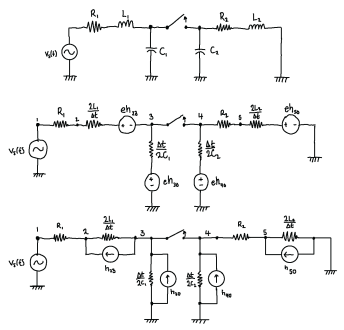
\includegraphics[width=5in]{schematic.png}
\caption{Transmission line's equivalent circuit and derivation of discretized components.}
\label{hand-setup}
\end{figure}

Once the current source histories are determined, the branch currents, which are required values for calculating the next nodal voltage values, can be calculated using the following relationships:

\begin{alignat}{2}
i_{23}(t) &= v_{23}(t)/R_{23} - h_{23}(t) \\
i_{30}(t) &= v_{30}(t)/R_{30} - h_{30}(t) \\
i_{40}(t) &= v_{40}(t)/R_{40} - h_{40}(t) \\
i_{50}(t) &= v_{50}(t)/R_{50} - h_{50}(t)
\end{alignat}

For this exercise, the convention used for currents leaving the node marks them as positive and currents entering the node marks them as negative. Therefore the resulting branch currents are the nodal voltage divided by the branch resistance, minus the discretized component current sources for all branch currents in this circuit.

Finally, we can now calculate the nodal voltage equations using some clever matrix manipulation taught in class. This technique subdivides the usual nodal analysis conductance matrix into four sections, with nodes connected to known voltage sources occupying the outside matrices $\mathbf{G_{AB}}$, $\mathbf{G_{BA}}$, and $\mathbf{G_{BB}}$. This allows us to perform the following operation to obtain our nodal voltage equation vector:

\begin{alignat}{2}
\left[\mathbf{V_A(t)}\right] &= \left[\mathbf{G_{AA}}\right]^{-1}\left[\mathbf{h_A(t)}\right] - \left[\mathbf{G_{AA}}\right]^{-1}\left[\mathbf{G_{AA}}\right]\left[\mathbf{V_B(t)}\right]
\end{alignat}

For this implementation, the breaker switch closing and opening has the effect of either connecting or breaking nodes 3 and 4 of the circuit (see Figure \ref{hand-setup} for node numbering). This has the result of generating two different conductance and history matrices. Shown below are both conductance and history matrices used for this circuit's solution:

\begin{alignat}{2}
  \left[
  \mathbf{G_{closed}}\right] &= \left[
      \begin{array}{c;{2pt/2pt}c}
        \mathbf{G_{AA}} & \mathbf{G_{AB}} \\ \hdashline[2pt/2pt]
        \mathbf{G_{BA}} & \mathbf{G_{BB}} 
      \end{array}
    \right] = \left[
      \begin{array}{ccc;{2pt/2pt}c}
        \frac{\Delta{}t}{2\,L_{1}}+\frac{1}{R_{1}} & -\frac{\Delta{}t}{2\,L_{1}} & 0 & -\frac{1}{R_{1}} \\ [6pt]
        -\frac{\Delta{}t}{2\,L_{1}} & \frac{2\,C_{1}}{\Delta{}t}+\frac{2\,C_{2}}{\Delta{}t}+\frac{\Delta{}t}{2\,L_{1}}+\frac{1}{R_{2}} & -\frac{1}{R_{2}} & 0 \\ [6pt]
        0 & -\frac{1}{R_{2}} & \frac{\Delta{}t}{2\,L_{2}}+\frac{1}{R_{2}} & 0 \\ [6pt] \hdashline[2pt/2pt]
        -\frac{1}{R_{1}} & 0 & 0 & \frac{1}{R_{1}}
      \end{array}
  \right] \\
  \left[
  \mathbf{G_{open}}\right] &= \left[
      \begin{array}{c;{2pt/2pt}c}
        \mathbf{G_{AA}} & \mathbf{G_{AB}} \\ \hdashline[2pt/2pt]
        \mathbf{G_{BA}} & \mathbf{G_{BB}} 
      \end{array}
    \right] = \left[\begin{array}{cccc;{2pt/2pt}c} \frac{\Delta{}t}{2\,L_{1}}+\frac{1}{R_{1}} & -\frac{\Delta{}t}{2\,L_{1}} & 0 & 0 & -\frac{1}{R_{1}} \\ [6pt]
    -\frac{\Delta{}t}{2\,L_{1}} & \frac{2\,C_{1}}{\Delta{}t}+\frac{\Delta{}t}{2\,L_{1}} & 0 & 0 & 0 \\ [6pt]
    0 & 0 & \frac{2\,C_{2}}{\Delta{}t}+\frac{1}{R_{2}} & -\frac{1}{R_{2}} & 0 \\ [6pt]
    0 & 0 & -\frac{1}{R_{2}} & \frac{\Delta{}t}{2\,L_{2}}+\frac{1}{R_{2}} & 0 \\ [6pt] \hdashline[2pt/2pt]
    -\frac{1}{R_{1}} & 0 & 0 & 0 & \frac{1}{R_{1}} \end{array}\right]
\end{alignat}

\begin{alignat}{2}
  \left[\mathbf{H_{closed}}\right] &= \left[\begin{array}{c} \mathbf{H_{A}} \\ \hdashline[2pt/2pt] \mathbf{H_{B}} \end{array}\right] = \left[\begin{array}{c} h_{23}(t) \\ -h_{23}(t) + h_{30}(t) + h_{40}(t) \\ h_{50}(t) \\ \hdashline[2pt/2pt] 0 \end{array}\right] \\
  \left[\mathbf{H_{open}}\right] &= \left[\begin{array}{c} \mathbf{H_{A}} \\ \hdashline[2pt/2pt] \mathbf{H_{B}} \end{array}\right] = \left[\begin{array}{c} h_{23}(t) \\ -h_{23}(t) + h_{30}(t) \\ h_{40}(t) \\ h_{50}(t) \\ \hdashline[2pt/2pt] 0 \end{array}\right]
\end{alignat}

The resulting nodal voltage equations were generated using MATLAB to minimize algebraic errors; the equations used to generate the nodal voltage equations were saved into a MATLAB file which can be viewed in Listing \ref{code-listing-matlab}. The resulting equations were then ported to a Python script which is provided in Listing \ref{code-listing-python}). There are two sets of nodal voltage solutions, one for the closed breaker and another for the open breaker. The closed breaker solution is used to begin with. Initial conditions are assumed to be zero for all variables. For each time step, the Python script then calculates the next nodal voltage value. These values are then used to calculate the next branch currents. After calculating the branch currents, the Python script checks if the breaker should have activated and if so, checks if the breaker current has changed sign since the last iteration. If both of these conditions are true, the breaker opens, effectively avoiding chopping current, and the open breaker solutions are used to calculate the nodal voltages until the end of the simulation. These results are plotted alongside the equivalent PSCAD solution for comparison using the Python matplotlib plotting library.

\subsection{Choosing a Simulation Time Step}

In order to choose an appropriate $\Delta{}t$ to simulate the circuit with, both sides of the circuit were analyzed for their resonant frequencies. This was performed by the following calculations:

\begin{alignat}{2}
f_{left} &= \frac{1}{2\pi\sqrt{L_1C_1}} = 2.69\,kHz \\
f_{right} &= \frac{1}{2\pi\sqrt{L_2C_2}} = 650\,Hz
\end{alignat}

The higher of the two frequencies, $2.69\,kHz$, corresponds to a period of $372\,\mu{}s$, so in order to get a good simulation result, an order of magnitude higher was chosen, at $\Delta{}t = 10\,\mu{}s$. 10 was chosen because it was a nice even number.

\subsection{PSCAD Simulation}

PSCAD provides a master library of components as well as primitives to help model the circuit. The resulting PSCAD circuit is shown in Figure \ref{pscad-setup}. The "Single Phase Voltage Source Model" component was used as the source and it was made ideal by setting the source impedance to $0 \Omega{}$ with a ramp-up time of $0 s$ (instantaneous voltage). The frequency was set to 60 Hz with a magnitude of $\frac{230}{\sqrt{2}}\,kV_{rms}$ and an offset of 90 degrees to match the assignment's voltage source equation of $230cos(377t)\,kV$. The ideal resistor, inductor, and capacitor were used to model the passive components and a series of voltmeters and ammeters were placed around the circuit to match the hand implemented solution. The voltage and current readings were piped to a plot on the same page as the schematic. In order to determine when PSCAD's breaker opened, the breaker's state variable was observed by plotting its value, and the resulting data is observed for a change that corresponds to an open state. The Python program plots both breaker opening times for the hand-implemented and PSCAD solutions (which turned out to be identical).

Once all of the components were hooked together and instrumented, the build button was clicked. This generated a Fortran program that models the entire circuit. A listing of this program can be found in Section \ref{code-listing-fortran}.

Clicking the run button ran the simulation and outputted the results on the plots. The data was extracted by right-clicking each plot{} to save it to the clipboard. This was then pasted into a CSV file for the Python program to read in as raw values.

\begin{figure}[H]
\centering
\includegraphics[width=5in]{pscad_schematic.png}
\caption{PSCAD schematic of transmission line.}
\label{pscad-setup}
\end{figure}

\section{Simulation}

With the hand-implemented and PSCAD solutions complete, the results can then be simulated and compared. This assignment requests the following comparison plots along with a zoomed-in portion for analysis. The figures following contain all of the plots required for the assignment.

\begin{enumerate}[label=\alph*)]
  \item Plots of $V_1$, $V_2$, $V_3$ for the simulation and PSCAD (Figures \ref{nodal_v_plots} and \ref{nodal_v_plots_zoom}).
  \item Plots of $I_{40}$ which represents the short-circuit current at the end of the transmission line (Figures \ref{short_circuit_i_plots} and \ref{short_circuit_i_plots_zoom}).
  \item Plots of $V_{23}$ which represents the voltage across the breaker (Figures \ref{breaker_v_plots} and \ref{breaker_v_plots_zoom}).
\end{enumerate}

Plots named simulation refer to the hand-modeled circuit and those named PSCAD refer to the PSCAD modeled circuit. In each plot, the red dashed line represents where the breaker has opened in the solution, which was identical between the hand-simulated and PSCAD solutions.

\begin{figure}[H]
    \begin{center}
        %% Creator: Matplotlib, PGF backend
%%
%% To include the figure in your LaTeX document, write
%%   \input{<filename>.pgf}
%%
%% Make sure the required packages are loaded in your preamble
%%   \usepackage{pgf}
%%
%% Figures using additional raster images can only be included by \input if
%% they are in the same directory as the main LaTeX file. For loading figures
%% from other directories you can use the `import` package
%%   \usepackage{import}
%% and then include the figures with
%%   \import{<path to file>}{<filename>.pgf}
%%
%% Matplotlib used the following preamble
%%
\begingroup%
\makeatletter%
\begin{pgfpicture}%
\pgfpathrectangle{\pgfpointorigin}{\pgfqpoint{6.500000in}{3.500000in}}%
\pgfusepath{use as bounding box}%
\begin{pgfscope}%
\pgfsetbuttcap%
\pgfsetroundjoin%
\definecolor{currentfill}{rgb}{1.000000,1.000000,1.000000}%
\pgfsetfillcolor{currentfill}%
\pgfsetlinewidth{0.000000pt}%
\definecolor{currentstroke}{rgb}{1.000000,1.000000,1.000000}%
\pgfsetstrokecolor{currentstroke}%
\pgfsetdash{}{0pt}%
\pgfpathmoveto{\pgfqpoint{0.000000in}{0.000000in}}%
\pgfpathlineto{\pgfqpoint{6.500000in}{0.000000in}}%
\pgfpathlineto{\pgfqpoint{6.500000in}{3.500000in}}%
\pgfpathlineto{\pgfqpoint{0.000000in}{3.500000in}}%
\pgfpathclose%
\pgfusepath{fill}%
\end{pgfscope}%
\begin{pgfscope}%
\pgfsetbuttcap%
\pgfsetroundjoin%
\definecolor{currentfill}{rgb}{1.000000,1.000000,1.000000}%
\pgfsetfillcolor{currentfill}%
\pgfsetlinewidth{0.000000pt}%
\definecolor{currentstroke}{rgb}{0.000000,0.000000,0.000000}%
\pgfsetstrokecolor{currentstroke}%
\pgfsetstrokeopacity{0.000000}%
\pgfsetdash{}{0pt}%
\pgfpathmoveto{\pgfqpoint{0.730248in}{0.537346in}}%
\pgfpathlineto{\pgfqpoint{6.157098in}{0.537346in}}%
\pgfpathlineto{\pgfqpoint{6.157098in}{3.164815in}}%
\pgfpathlineto{\pgfqpoint{0.730248in}{3.164815in}}%
\pgfpathclose%
\pgfusepath{fill}%
\end{pgfscope}%
\begin{pgfscope}%
\pgfpathrectangle{\pgfqpoint{0.730248in}{0.537346in}}{\pgfqpoint{5.426850in}{2.627470in}} %
\pgfusepath{clip}%
\pgfsetrectcap%
\pgfsetroundjoin%
\pgfsetlinewidth{1.003750pt}%
\definecolor{currentstroke}{rgb}{0.000000,0.000000,1.000000}%
\pgfsetstrokecolor{currentstroke}%
\pgfsetdash{}{0pt}%
\pgfpathmoveto{\pgfqpoint{0.730519in}{2.606472in}}%
\pgfpathlineto{\pgfqpoint{0.734318in}{2.605270in}}%
\pgfpathlineto{\pgfqpoint{0.738660in}{2.601325in}}%
\pgfpathlineto{\pgfqpoint{0.743544in}{2.593625in}}%
\pgfpathlineto{\pgfqpoint{0.749513in}{2.579578in}}%
\pgfpathlineto{\pgfqpoint{0.756297in}{2.557542in}}%
\pgfpathlineto{\pgfqpoint{0.764166in}{2.524141in}}%
\pgfpathlineto{\pgfqpoint{0.773391in}{2.474780in}}%
\pgfpathlineto{\pgfqpoint{0.784245in}{2.403678in}}%
\pgfpathlineto{\pgfqpoint{0.796998in}{2.304243in}}%
\pgfpathlineto{\pgfqpoint{0.812465in}{2.164944in}}%
\pgfpathlineto{\pgfqpoint{0.833901in}{1.949497in}}%
\pgfpathlineto{\pgfqpoint{0.878944in}{1.492134in}}%
\pgfpathlineto{\pgfqpoint{0.895224in}{1.352209in}}%
\pgfpathlineto{\pgfqpoint{0.908249in}{1.258268in}}%
\pgfpathlineto{\pgfqpoint{0.919374in}{1.193256in}}%
\pgfpathlineto{\pgfqpoint{0.928871in}{1.150118in}}%
\pgfpathlineto{\pgfqpoint{0.937011in}{1.122820in}}%
\pgfpathlineto{\pgfqpoint{0.943794in}{1.107168in}}%
\pgfpathlineto{\pgfqpoint{0.949493in}{1.099120in}}%
\pgfpathlineto{\pgfqpoint{0.954105in}{1.096054in}}%
\pgfpathlineto{\pgfqpoint{0.958176in}{1.095923in}}%
\pgfpathlineto{\pgfqpoint{0.962246in}{1.098206in}}%
\pgfpathlineto{\pgfqpoint{0.966859in}{1.103703in}}%
\pgfpathlineto{\pgfqpoint{0.972285in}{1.114096in}}%
\pgfpathlineto{\pgfqpoint{0.978526in}{1.131221in}}%
\pgfpathlineto{\pgfqpoint{0.985853in}{1.158214in}}%
\pgfpathlineto{\pgfqpoint{0.994536in}{1.199466in}}%
\pgfpathlineto{\pgfqpoint{1.004575in}{1.258926in}}%
\pgfpathlineto{\pgfqpoint{1.016243in}{1.342390in}}%
\pgfpathlineto{\pgfqpoint{1.030081in}{1.458475in}}%
\pgfpathlineto{\pgfqpoint{1.047719in}{1.626771in}}%
\pgfpathlineto{\pgfqpoint{1.079737in}{1.959012in}}%
\pgfpathlineto{\pgfqpoint{1.104701in}{2.206731in}}%
\pgfpathlineto{\pgfqpoint{1.120981in}{2.347136in}}%
\pgfpathlineto{\pgfqpoint{1.134006in}{2.441567in}}%
\pgfpathlineto{\pgfqpoint{1.145131in}{2.507058in}}%
\pgfpathlineto{\pgfqpoint{1.154628in}{2.550640in}}%
\pgfpathlineto{\pgfqpoint{1.162768in}{2.578338in}}%
\pgfpathlineto{\pgfqpoint{1.169551in}{2.594333in}}%
\pgfpathlineto{\pgfqpoint{1.175250in}{2.602675in}}%
\pgfpathlineto{\pgfqpoint{1.179862in}{2.605980in}}%
\pgfpathlineto{\pgfqpoint{1.183933in}{2.606323in}}%
\pgfpathlineto{\pgfqpoint{1.188003in}{2.604251in}}%
\pgfpathlineto{\pgfqpoint{1.192344in}{2.599387in}}%
\pgfpathlineto{\pgfqpoint{1.197500in}{2.590078in}}%
\pgfpathlineto{\pgfqpoint{1.203741in}{2.573744in}}%
\pgfpathlineto{\pgfqpoint{1.211067in}{2.547652in}}%
\pgfpathlineto{\pgfqpoint{1.219478in}{2.508823in}}%
\pgfpathlineto{\pgfqpoint{1.229247in}{2.452511in}}%
\pgfpathlineto{\pgfqpoint{1.240643in}{2.372918in}}%
\pgfpathlineto{\pgfqpoint{1.254210in}{2.261328in}}%
\pgfpathlineto{\pgfqpoint{1.271034in}{2.103260in}}%
\pgfpathlineto{\pgfqpoint{1.297625in}{1.829110in}}%
\pgfpathlineto{\pgfqpoint{1.328287in}{1.519045in}}%
\pgfpathlineto{\pgfqpoint{1.345110in}{1.370919in}}%
\pgfpathlineto{\pgfqpoint{1.358677in}{1.270149in}}%
\pgfpathlineto{\pgfqpoint{1.370074in}{1.201281in}}%
\pgfpathlineto{\pgfqpoint{1.379842in}{1.155136in}}%
\pgfpathlineto{\pgfqpoint{1.387982in}{1.126431in}}%
\pgfpathlineto{\pgfqpoint{1.395037in}{1.109032in}}%
\pgfpathlineto{\pgfqpoint{1.400735in}{1.100175in}}%
\pgfpathlineto{\pgfqpoint{1.405619in}{1.096325in}}%
\pgfpathlineto{\pgfqpoint{1.409690in}{1.095771in}}%
\pgfpathlineto{\pgfqpoint{1.413760in}{1.097632in}}%
\pgfpathlineto{\pgfqpoint{1.418101in}{1.102271in}}%
\pgfpathlineto{\pgfqpoint{1.423257in}{1.111316in}}%
\pgfpathlineto{\pgfqpoint{1.429226in}{1.126525in}}%
\pgfpathlineto{\pgfqpoint{1.436281in}{1.150912in}}%
\pgfpathlineto{\pgfqpoint{1.444421in}{1.187384in}}%
\pgfpathlineto{\pgfqpoint{1.453918in}{1.240615in}}%
\pgfpathlineto{\pgfqpoint{1.465043in}{1.316391in}}%
\pgfpathlineto{\pgfqpoint{1.478068in}{1.421157in}}%
\pgfpathlineto{\pgfqpoint{1.494348in}{1.571411in}}%
\pgfpathlineto{\pgfqpoint{1.518227in}{1.815217in}}%
\pgfpathlineto{\pgfqpoint{1.554586in}{2.184870in}}%
\pgfpathlineto{\pgfqpoint{1.571410in}{2.332749in}}%
\pgfpathlineto{\pgfqpoint{1.584977in}{2.433259in}}%
\pgfpathlineto{\pgfqpoint{1.596373in}{2.501874in}}%
\pgfpathlineto{\pgfqpoint{1.606142in}{2.547782in}}%
\pgfpathlineto{\pgfqpoint{1.614282in}{2.576280in}}%
\pgfpathlineto{\pgfqpoint{1.621337in}{2.593492in}}%
\pgfpathlineto{\pgfqpoint{1.627035in}{2.602196in}}%
\pgfpathlineto{\pgfqpoint{1.631919in}{2.605913in}}%
\pgfpathlineto{\pgfqpoint{1.635989in}{2.606357in}}%
\pgfpathlineto{\pgfqpoint{1.640059in}{2.604386in}}%
\pgfpathlineto{\pgfqpoint{1.644401in}{2.599629in}}%
\pgfpathlineto{\pgfqpoint{1.649556in}{2.590446in}}%
\pgfpathlineto{\pgfqpoint{1.655797in}{2.574262in}}%
\pgfpathlineto{\pgfqpoint{1.663123in}{2.548342in}}%
\pgfpathlineto{\pgfqpoint{1.671535in}{2.509700in}}%
\pgfpathlineto{\pgfqpoint{1.681303in}{2.453590in}}%
\pgfpathlineto{\pgfqpoint{1.692700in}{2.374209in}}%
\pgfpathlineto{\pgfqpoint{1.706267in}{2.262828in}}%
\pgfpathlineto{\pgfqpoint{1.723090in}{2.104944in}}%
\pgfpathlineto{\pgfqpoint{1.749682in}{1.830896in}}%
\pgfpathlineto{\pgfqpoint{1.780343in}{1.520651in}}%
\pgfpathlineto{\pgfqpoint{1.797167in}{1.372300in}}%
\pgfpathlineto{\pgfqpoint{1.810734in}{1.271293in}}%
\pgfpathlineto{\pgfqpoint{1.822130in}{1.202194in}}%
\pgfpathlineto{\pgfqpoint{1.831899in}{1.155833in}}%
\pgfpathlineto{\pgfqpoint{1.840310in}{1.126132in}}%
\pgfpathlineto{\pgfqpoint{1.847365in}{1.108834in}}%
\pgfpathlineto{\pgfqpoint{1.853063in}{1.100060in}}%
\pgfpathlineto{\pgfqpoint{1.857947in}{1.096282in}}%
\pgfpathlineto{\pgfqpoint{1.862018in}{1.095788in}}%
\pgfpathlineto{\pgfqpoint{1.866088in}{1.097709in}}%
\pgfpathlineto{\pgfqpoint{1.870429in}{1.102412in}}%
\pgfpathlineto{\pgfqpoint{1.875585in}{1.111532in}}%
\pgfpathlineto{\pgfqpoint{1.881826in}{1.127641in}}%
\pgfpathlineto{\pgfqpoint{1.888880in}{1.152388in}}%
\pgfpathlineto{\pgfqpoint{1.897292in}{1.190637in}}%
\pgfpathlineto{\pgfqpoint{1.907060in}{1.246321in}}%
\pgfpathlineto{\pgfqpoint{1.918457in}{1.325260in}}%
\pgfpathlineto{\pgfqpoint{1.931753in}{1.433825in}}%
\pgfpathlineto{\pgfqpoint{1.948304in}{1.588349in}}%
\pgfpathlineto{\pgfqpoint{1.973811in}{1.850439in}}%
\pgfpathlineto{\pgfqpoint{2.006372in}{2.180706in}}%
\pgfpathlineto{\pgfqpoint{2.023195in}{2.329170in}}%
\pgfpathlineto{\pgfqpoint{2.036762in}{2.430295in}}%
\pgfpathlineto{\pgfqpoint{2.048159in}{2.499509in}}%
\pgfpathlineto{\pgfqpoint{2.057927in}{2.545978in}}%
\pgfpathlineto{\pgfqpoint{2.066338in}{2.575777in}}%
\pgfpathlineto{\pgfqpoint{2.073393in}{2.593160in}}%
\pgfpathlineto{\pgfqpoint{2.079092in}{2.602004in}}%
\pgfpathlineto{\pgfqpoint{2.083976in}{2.605842in}}%
\pgfpathlineto{\pgfqpoint{2.088046in}{2.606387in}}%
\pgfpathlineto{\pgfqpoint{2.092116in}{2.604517in}}%
\pgfpathlineto{\pgfqpoint{2.096457in}{2.599867in}}%
\pgfpathlineto{\pgfqpoint{2.101613in}{2.590810in}}%
\pgfpathlineto{\pgfqpoint{2.107583in}{2.575588in}}%
\pgfpathlineto{\pgfqpoint{2.114637in}{2.551186in}}%
\pgfpathlineto{\pgfqpoint{2.122778in}{2.514697in}}%
\pgfpathlineto{\pgfqpoint{2.132275in}{2.461447in}}%
\pgfpathlineto{\pgfqpoint{2.143400in}{2.385651in}}%
\pgfpathlineto{\pgfqpoint{2.156424in}{2.280866in}}%
\pgfpathlineto{\pgfqpoint{2.172705in}{2.130594in}}%
\pgfpathlineto{\pgfqpoint{2.196583in}{1.886776in}}%
\pgfpathlineto{\pgfqpoint{2.232943in}{1.517140in}}%
\pgfpathlineto{\pgfqpoint{2.249766in}{1.369282in}}%
\pgfpathlineto{\pgfqpoint{2.263333in}{1.268795in}}%
\pgfpathlineto{\pgfqpoint{2.274730in}{1.200201in}}%
\pgfpathlineto{\pgfqpoint{2.284498in}{1.154314in}}%
\pgfpathlineto{\pgfqpoint{2.292638in}{1.125834in}}%
\pgfpathlineto{\pgfqpoint{2.299693in}{1.108638in}}%
\pgfpathlineto{\pgfqpoint{2.305391in}{1.099947in}}%
\pgfpathlineto{\pgfqpoint{2.310275in}{1.096241in}}%
\pgfpathlineto{\pgfqpoint{2.314346in}{1.095807in}}%
\pgfpathlineto{\pgfqpoint{2.318416in}{1.097787in}}%
\pgfpathlineto{\pgfqpoint{2.322757in}{1.102554in}}%
\pgfpathlineto{\pgfqpoint{2.327913in}{1.111749in}}%
\pgfpathlineto{\pgfqpoint{2.334154in}{1.127947in}}%
\pgfpathlineto{\pgfqpoint{2.341480in}{1.153883in}}%
\pgfpathlineto{\pgfqpoint{2.349891in}{1.192543in}}%
\pgfpathlineto{\pgfqpoint{2.359660in}{1.248671in}}%
\pgfpathlineto{\pgfqpoint{2.371056in}{1.328073in}}%
\pgfpathlineto{\pgfqpoint{2.384623in}{1.439474in}}%
\pgfpathlineto{\pgfqpoint{2.401446in}{1.597375in}}%
\pgfpathlineto{\pgfqpoint{2.428038in}{1.871432in}}%
\pgfpathlineto{\pgfqpoint{2.458700in}{2.181661in}}%
\pgfpathlineto{\pgfqpoint{2.475523in}{2.329991in}}%
\pgfpathlineto{\pgfqpoint{2.489090in}{2.430975in}}%
\pgfpathlineto{\pgfqpoint{2.500486in}{2.500053in}}%
\pgfpathlineto{\pgfqpoint{2.510255in}{2.546393in}}%
\pgfpathlineto{\pgfqpoint{2.518666in}{2.576076in}}%
\pgfpathlineto{\pgfqpoint{2.525721in}{2.593357in}}%
\pgfpathlineto{\pgfqpoint{2.531420in}{2.602119in}}%
\pgfpathlineto{\pgfqpoint{2.536304in}{2.605885in}}%
\pgfpathlineto{\pgfqpoint{2.540374in}{2.606370in}}%
\pgfpathlineto{\pgfqpoint{2.544444in}{2.604440in}}%
\pgfpathlineto{\pgfqpoint{2.548785in}{2.599726in}}%
\pgfpathlineto{\pgfqpoint{2.553941in}{2.590595in}}%
\pgfpathlineto{\pgfqpoint{2.560182in}{2.574472in}}%
\pgfpathlineto{\pgfqpoint{2.567237in}{2.549709in}}%
\pgfpathlineto{\pgfqpoint{2.575648in}{2.511442in}}%
\pgfpathlineto{\pgfqpoint{2.585417in}{2.455739in}}%
\pgfpathlineto{\pgfqpoint{2.596813in}{2.376781in}}%
\pgfpathlineto{\pgfqpoint{2.610109in}{2.268196in}}%
\pgfpathlineto{\pgfqpoint{2.626661in}{2.113655in}}%
\pgfpathlineto{\pgfqpoint{2.652167in}{1.851554in}}%
\pgfpathlineto{\pgfqpoint{2.684728in}{1.521303in}}%
\pgfpathlineto{\pgfqpoint{2.701551in}{1.372861in}}%
\pgfpathlineto{\pgfqpoint{2.715118in}{1.271758in}}%
\pgfpathlineto{\pgfqpoint{2.726515in}{1.202566in}}%
\pgfpathlineto{\pgfqpoint{2.736283in}{1.156117in}}%
\pgfpathlineto{\pgfqpoint{2.744695in}{1.126336in}}%
\pgfpathlineto{\pgfqpoint{2.751750in}{1.108970in}}%
\pgfpathlineto{\pgfqpoint{2.757448in}{1.100138in}}%
\pgfpathlineto{\pgfqpoint{2.762332in}{1.096312in}}%
\pgfpathlineto{\pgfqpoint{2.766402in}{1.095776in}}%
\pgfpathlineto{\pgfqpoint{2.770472in}{1.097656in}}%
\pgfpathlineto{\pgfqpoint{2.774814in}{1.102316in}}%
\pgfpathlineto{\pgfqpoint{2.779969in}{1.111384in}}%
\pgfpathlineto{\pgfqpoint{2.785939in}{1.126620in}}%
\pgfpathlineto{\pgfqpoint{2.792994in}{1.151038in}}%
\pgfpathlineto{\pgfqpoint{2.801134in}{1.187544in}}%
\pgfpathlineto{\pgfqpoint{2.810631in}{1.240812in}}%
\pgfpathlineto{\pgfqpoint{2.821756in}{1.316628in}}%
\pgfpathlineto{\pgfqpoint{2.834780in}{1.421433in}}%
\pgfpathlineto{\pgfqpoint{2.851061in}{1.571723in}}%
\pgfpathlineto{\pgfqpoint{2.874939in}{1.815552in}}%
\pgfpathlineto{\pgfqpoint{2.911299in}{2.185171in}}%
\pgfpathlineto{\pgfqpoint{2.928122in}{2.333007in}}%
\pgfpathlineto{\pgfqpoint{2.941689in}{2.433473in}}%
\pgfpathlineto{\pgfqpoint{2.953086in}{2.502044in}}%
\pgfpathlineto{\pgfqpoint{2.962854in}{2.547912in}}%
\pgfpathlineto{\pgfqpoint{2.970994in}{2.576373in}}%
\pgfpathlineto{\pgfqpoint{2.978049in}{2.593554in}}%
\pgfpathlineto{\pgfqpoint{2.983747in}{2.602232in}}%
\pgfpathlineto{\pgfqpoint{2.988632in}{2.605926in}}%
\pgfpathlineto{\pgfqpoint{2.992702in}{2.606351in}}%
\pgfpathlineto{\pgfqpoint{2.996772in}{2.604361in}}%
\pgfpathlineto{\pgfqpoint{3.001113in}{2.599584in}}%
\pgfpathlineto{\pgfqpoint{3.006269in}{2.590377in}}%
\pgfpathlineto{\pgfqpoint{3.012510in}{2.574165in}}%
\pgfpathlineto{\pgfqpoint{3.019836in}{2.548213in}}%
\pgfpathlineto{\pgfqpoint{3.028248in}{2.509535in}}%
\pgfpathlineto{\pgfqpoint{3.038016in}{2.453388in}}%
\pgfpathlineto{\pgfqpoint{3.049412in}{2.373966in}}%
\pgfpathlineto{\pgfqpoint{3.062980in}{2.262546in}}%
\pgfpathlineto{\pgfqpoint{3.079803in}{2.104628in}}%
\pgfpathlineto{\pgfqpoint{3.106394in}{1.830561in}}%
\pgfpathlineto{\pgfqpoint{3.137056in}{1.520349in}}%
\pgfpathlineto{\pgfqpoint{3.153879in}{1.372040in}}%
\pgfpathlineto{\pgfqpoint{3.167446in}{1.271078in}}%
\pgfpathlineto{\pgfqpoint{3.178843in}{1.202022in}}%
\pgfpathlineto{\pgfqpoint{3.188611in}{1.155702in}}%
\pgfpathlineto{\pgfqpoint{3.197023in}{1.126037in}}%
\pgfpathlineto{\pgfqpoint{3.204078in}{1.108772in}}%
\pgfpathlineto{\pgfqpoint{3.209776in}{1.100024in}}%
\pgfpathlineto{\pgfqpoint{3.214660in}{1.096269in}}%
\pgfpathlineto{\pgfqpoint{3.218730in}{1.095794in}}%
\pgfpathlineto{\pgfqpoint{3.222800in}{1.097734in}}%
\pgfpathlineto{\pgfqpoint{3.227142in}{1.102457in}}%
\pgfpathlineto{\pgfqpoint{3.232297in}{1.111600in}}%
\pgfpathlineto{\pgfqpoint{3.238538in}{1.127737in}}%
\pgfpathlineto{\pgfqpoint{3.245593in}{1.152516in}}%
\pgfpathlineto{\pgfqpoint{3.254005in}{1.190800in}}%
\pgfpathlineto{\pgfqpoint{3.263773in}{1.246522in}}%
\pgfpathlineto{\pgfqpoint{3.275169in}{1.325501in}}%
\pgfpathlineto{\pgfqpoint{3.288465in}{1.434104in}}%
\pgfpathlineto{\pgfqpoint{3.305017in}{1.588663in}}%
\pgfpathlineto{\pgfqpoint{3.330523in}{1.850774in}}%
\pgfpathlineto{\pgfqpoint{3.363084in}{2.181008in}}%
\pgfpathlineto{\pgfqpoint{3.379908in}{2.329430in}}%
\pgfpathlineto{\pgfqpoint{3.393475in}{2.430510in}}%
\pgfpathlineto{\pgfqpoint{3.404871in}{2.499681in}}%
\pgfpathlineto{\pgfqpoint{3.414639in}{2.546109in}}%
\pgfpathlineto{\pgfqpoint{3.423051in}{2.575872in}}%
\pgfpathlineto{\pgfqpoint{3.430106in}{2.593222in}}%
\pgfpathlineto{\pgfqpoint{3.435804in}{2.602041in}}%
\pgfpathlineto{\pgfqpoint{3.440688in}{2.605856in}}%
\pgfpathlineto{\pgfqpoint{3.444758in}{2.606382in}}%
\pgfpathlineto{\pgfqpoint{3.448829in}{2.604492in}}%
\pgfpathlineto{\pgfqpoint{3.453170in}{2.599823in}}%
\pgfpathlineto{\pgfqpoint{3.458326in}{2.590742in}}%
\pgfpathlineto{\pgfqpoint{3.464295in}{2.575493in}}%
\pgfpathlineto{\pgfqpoint{3.471350in}{2.551060in}}%
\pgfpathlineto{\pgfqpoint{3.479490in}{2.514536in}}%
\pgfpathlineto{\pgfqpoint{3.488987in}{2.461249in}}%
\pgfpathlineto{\pgfqpoint{3.500112in}{2.385414in}}%
\pgfpathlineto{\pgfqpoint{3.513137in}{2.280590in}}%
\pgfpathlineto{\pgfqpoint{3.529417in}{2.130282in}}%
\pgfpathlineto{\pgfqpoint{3.553295in}{1.886441in}}%
\pgfpathlineto{\pgfqpoint{3.589655in}{1.516839in}}%
\pgfpathlineto{\pgfqpoint{3.606479in}{1.369024in}}%
\pgfpathlineto{\pgfqpoint{3.620046in}{1.268581in}}%
\pgfpathlineto{\pgfqpoint{3.631442in}{1.200031in}}%
\pgfpathlineto{\pgfqpoint{3.641210in}{1.154184in}}%
\pgfpathlineto{\pgfqpoint{3.649351in}{1.125740in}}%
\pgfpathlineto{\pgfqpoint{3.656406in}{1.108576in}}%
\pgfpathlineto{\pgfqpoint{3.662104in}{1.099911in}}%
\pgfpathlineto{\pgfqpoint{3.666988in}{1.096228in}}%
\pgfpathlineto{\pgfqpoint{3.671058in}{1.095813in}}%
\pgfpathlineto{\pgfqpoint{3.675128in}{1.097812in}}%
\pgfpathlineto{\pgfqpoint{3.679470in}{1.102599in}}%
\pgfpathlineto{\pgfqpoint{3.684625in}{1.111818in}}%
\pgfpathlineto{\pgfqpoint{3.690866in}{1.128044in}}%
\pgfpathlineto{\pgfqpoint{3.698192in}{1.154013in}}%
\pgfpathlineto{\pgfqpoint{3.706604in}{1.192708in}}%
\pgfpathlineto{\pgfqpoint{3.716372in}{1.248874in}}%
\pgfpathlineto{\pgfqpoint{3.727769in}{1.328315in}}%
\pgfpathlineto{\pgfqpoint{3.741336in}{1.439755in}}%
\pgfpathlineto{\pgfqpoint{3.758159in}{1.597691in}}%
\pgfpathlineto{\pgfqpoint{3.784751in}{1.871767in}}%
\pgfpathlineto{\pgfqpoint{3.815412in}{2.181962in}}%
\pgfpathlineto{\pgfqpoint{3.832236in}{2.330250in}}%
\pgfpathlineto{\pgfqpoint{3.845803in}{2.431190in}}%
\pgfpathlineto{\pgfqpoint{3.857199in}{2.500224in}}%
\pgfpathlineto{\pgfqpoint{3.866967in}{2.546524in}}%
\pgfpathlineto{\pgfqpoint{3.875108in}{2.575367in}}%
\pgfpathlineto{\pgfqpoint{3.882163in}{2.592887in}}%
\pgfpathlineto{\pgfqpoint{3.887861in}{2.601845in}}%
\pgfpathlineto{\pgfqpoint{3.892745in}{2.605781in}}%
\pgfpathlineto{\pgfqpoint{3.896815in}{2.606408in}}%
\pgfpathlineto{\pgfqpoint{3.900614in}{2.604814in}}%
\pgfpathlineto{\pgfqpoint{3.904955in}{2.600423in}}%
\pgfpathlineto{\pgfqpoint{3.910111in}{2.591669in}}%
\pgfpathlineto{\pgfqpoint{3.916080in}{2.576793in}}%
\pgfpathlineto{\pgfqpoint{3.923135in}{2.552789in}}%
\pgfpathlineto{\pgfqpoint{3.931276in}{2.516740in}}%
\pgfpathlineto{\pgfqpoint{3.940773in}{2.463970in}}%
\pgfpathlineto{\pgfqpoint{3.951898in}{2.388680in}}%
\pgfpathlineto{\pgfqpoint{3.964922in}{2.284395in}}%
\pgfpathlineto{\pgfqpoint{3.980931in}{2.137221in}}%
\pgfpathlineto{\pgfqpoint{4.004267in}{1.899599in}}%
\pgfpathlineto{\pgfqpoint{4.042255in}{1.513338in}}%
\pgfpathlineto{\pgfqpoint{4.059078in}{1.366021in}}%
\pgfpathlineto{\pgfqpoint{4.072374in}{1.267906in}}%
\pgfpathlineto{\pgfqpoint{4.083770in}{1.199494in}}%
\pgfpathlineto{\pgfqpoint{4.093538in}{1.153775in}}%
\pgfpathlineto{\pgfqpoint{4.101679in}{1.125445in}}%
\pgfpathlineto{\pgfqpoint{4.108734in}{1.108382in}}%
\pgfpathlineto{\pgfqpoint{4.114432in}{1.099800in}}%
\pgfpathlineto{\pgfqpoint{4.119045in}{1.096298in}}%
\pgfpathlineto{\pgfqpoint{4.123115in}{1.095782in}}%
\pgfpathlineto{\pgfqpoint{4.127185in}{1.097680in}}%
\pgfpathlineto{\pgfqpoint{4.131526in}{1.102360in}}%
\pgfpathlineto{\pgfqpoint{4.136682in}{1.111453in}}%
\pgfpathlineto{\pgfqpoint{4.142651in}{1.126715in}}%
\pgfpathlineto{\pgfqpoint{4.149706in}{1.151164in}}%
\pgfpathlineto{\pgfqpoint{4.158118in}{1.189071in}}%
\pgfpathlineto{\pgfqpoint{4.167615in}{1.242694in}}%
\pgfpathlineto{\pgfqpoint{4.178740in}{1.318883in}}%
\pgfpathlineto{\pgfqpoint{4.192036in}{1.426407in}}%
\pgfpathlineto{\pgfqpoint{4.208316in}{1.577335in}}%
\pgfpathlineto{\pgfqpoint{4.232737in}{1.827270in}}%
\pgfpathlineto{\pgfqpoint{4.267740in}{2.182916in}}%
\pgfpathlineto{\pgfqpoint{4.284564in}{2.331070in}}%
\pgfpathlineto{\pgfqpoint{4.298131in}{2.431869in}}%
\pgfpathlineto{\pgfqpoint{4.309527in}{2.500766in}}%
\pgfpathlineto{\pgfqpoint{4.319295in}{2.546938in}}%
\pgfpathlineto{\pgfqpoint{4.327436in}{2.575667in}}%
\pgfpathlineto{\pgfqpoint{4.334491in}{2.593087in}}%
\pgfpathlineto{\pgfqpoint{4.340189in}{2.601962in}}%
\pgfpathlineto{\pgfqpoint{4.345073in}{2.605826in}}%
\pgfpathlineto{\pgfqpoint{4.349143in}{2.606393in}}%
\pgfpathlineto{\pgfqpoint{4.353213in}{2.604545in}}%
\pgfpathlineto{\pgfqpoint{4.357555in}{2.599919in}}%
\pgfpathlineto{\pgfqpoint{4.362710in}{2.590889in}}%
\pgfpathlineto{\pgfqpoint{4.368680in}{2.575698in}}%
\pgfpathlineto{\pgfqpoint{4.375735in}{2.551333in}}%
\pgfpathlineto{\pgfqpoint{4.383875in}{2.514883in}}%
\pgfpathlineto{\pgfqpoint{4.393372in}{2.461677in}}%
\pgfpathlineto{\pgfqpoint{4.404497in}{2.385927in}}%
\pgfpathlineto{\pgfqpoint{4.417521in}{2.281187in}}%
\pgfpathlineto{\pgfqpoint{4.433802in}{2.130956in}}%
\pgfpathlineto{\pgfqpoint{4.457680in}{1.887166in}}%
\pgfpathlineto{\pgfqpoint{4.494040in}{1.517490in}}%
\pgfpathlineto{\pgfqpoint{4.510863in}{1.369583in}}%
\pgfpathlineto{\pgfqpoint{4.524430in}{1.269044in}}%
\pgfpathlineto{\pgfqpoint{4.535827in}{1.200399in}}%
\pgfpathlineto{\pgfqpoint{4.545595in}{1.154465in}}%
\pgfpathlineto{\pgfqpoint{4.553735in}{1.125943in}}%
\pgfpathlineto{\pgfqpoint{4.560790in}{1.108710in}}%
\pgfpathlineto{\pgfqpoint{4.566488in}{1.099988in}}%
\pgfpathlineto{\pgfqpoint{4.571373in}{1.096256in}}%
\pgfpathlineto{\pgfqpoint{4.575443in}{1.095800in}}%
\pgfpathlineto{\pgfqpoint{4.579513in}{1.097758in}}%
\pgfpathlineto{\pgfqpoint{4.583854in}{1.102502in}}%
\pgfpathlineto{\pgfqpoint{4.589010in}{1.111669in}}%
\pgfpathlineto{\pgfqpoint{4.595251in}{1.127834in}}%
\pgfpathlineto{\pgfqpoint{4.602306in}{1.152643in}}%
\pgfpathlineto{\pgfqpoint{4.610717in}{1.190963in}}%
\pgfpathlineto{\pgfqpoint{4.620486in}{1.246723in}}%
\pgfpathlineto{\pgfqpoint{4.631882in}{1.325742in}}%
\pgfpathlineto{\pgfqpoint{4.645178in}{1.434384in}}%
\pgfpathlineto{\pgfqpoint{4.661730in}{1.588978in}}%
\pgfpathlineto{\pgfqpoint{4.687236in}{1.851109in}}%
\pgfpathlineto{\pgfqpoint{4.719797in}{2.181310in}}%
\pgfpathlineto{\pgfqpoint{4.736620in}{2.329689in}}%
\pgfpathlineto{\pgfqpoint{4.750187in}{2.430725in}}%
\pgfpathlineto{\pgfqpoint{4.761584in}{2.499853in}}%
\pgfpathlineto{\pgfqpoint{4.771352in}{2.546241in}}%
\pgfpathlineto{\pgfqpoint{4.779764in}{2.575966in}}%
\pgfpathlineto{\pgfqpoint{4.786818in}{2.593285in}}%
\pgfpathlineto{\pgfqpoint{4.792517in}{2.602077in}}%
\pgfpathlineto{\pgfqpoint{4.797401in}{2.605869in}}%
\pgfpathlineto{\pgfqpoint{4.801471in}{2.606376in}}%
\pgfpathlineto{\pgfqpoint{4.805541in}{2.604468in}}%
\pgfpathlineto{\pgfqpoint{4.809883in}{2.599778in}}%
\pgfpathlineto{\pgfqpoint{4.815038in}{2.590674in}}%
\pgfpathlineto{\pgfqpoint{4.821008in}{2.575398in}}%
\pgfpathlineto{\pgfqpoint{4.828063in}{2.550934in}}%
\pgfpathlineto{\pgfqpoint{4.836474in}{2.513008in}}%
\pgfpathlineto{\pgfqpoint{4.845971in}{2.459367in}}%
\pgfpathlineto{\pgfqpoint{4.857096in}{2.383159in}}%
\pgfpathlineto{\pgfqpoint{4.870392in}{2.275615in}}%
\pgfpathlineto{\pgfqpoint{4.886673in}{2.124669in}}%
\pgfpathlineto{\pgfqpoint{4.911093in}{1.874724in}}%
\pgfpathlineto{\pgfqpoint{4.946097in}{1.519094in}}%
\pgfpathlineto{\pgfqpoint{4.962920in}{1.370961in}}%
\pgfpathlineto{\pgfqpoint{4.976487in}{1.270184in}}%
\pgfpathlineto{\pgfqpoint{4.987883in}{1.201309in}}%
\pgfpathlineto{\pgfqpoint{4.997652in}{1.155157in}}%
\pgfpathlineto{\pgfqpoint{5.005792in}{1.126446in}}%
\pgfpathlineto{\pgfqpoint{5.012847in}{1.109042in}}%
\pgfpathlineto{\pgfqpoint{5.018545in}{1.100181in}}%
\pgfpathlineto{\pgfqpoint{5.023429in}{1.096328in}}%
\pgfpathlineto{\pgfqpoint{5.027499in}{1.095770in}}%
\pgfpathlineto{\pgfqpoint{5.031569in}{1.097628in}}%
\pgfpathlineto{\pgfqpoint{5.035911in}{1.102264in}}%
\pgfpathlineto{\pgfqpoint{5.041066in}{1.111305in}}%
\pgfpathlineto{\pgfqpoint{5.047036in}{1.126510in}}%
\pgfpathlineto{\pgfqpoint{5.054091in}{1.150891in}}%
\pgfpathlineto{\pgfqpoint{5.062231in}{1.187358in}}%
\pgfpathlineto{\pgfqpoint{5.071728in}{1.240583in}}%
\pgfpathlineto{\pgfqpoint{5.082853in}{1.316353in}}%
\pgfpathlineto{\pgfqpoint{5.095878in}{1.421112in}}%
\pgfpathlineto{\pgfqpoint{5.112158in}{1.571360in}}%
\pgfpathlineto{\pgfqpoint{5.136036in}{1.815162in}}%
\pgfpathlineto{\pgfqpoint{5.172396in}{2.184821in}}%
\pgfpathlineto{\pgfqpoint{5.189219in}{2.332707in}}%
\pgfpathlineto{\pgfqpoint{5.202787in}{2.433224in}}%
\pgfpathlineto{\pgfqpoint{5.214183in}{2.501846in}}%
\pgfpathlineto{\pgfqpoint{5.223951in}{2.547761in}}%
\pgfpathlineto{\pgfqpoint{5.232092in}{2.576264in}}%
\pgfpathlineto{\pgfqpoint{5.239146in}{2.593482in}}%
\pgfpathlineto{\pgfqpoint{5.244845in}{2.602190in}}%
\pgfpathlineto{\pgfqpoint{5.249729in}{2.605911in}}%
\pgfpathlineto{\pgfqpoint{5.253799in}{2.606358in}}%
\pgfpathlineto{\pgfqpoint{5.257869in}{2.604390in}}%
\pgfpathlineto{\pgfqpoint{5.262211in}{2.599637in}}%
\pgfpathlineto{\pgfqpoint{5.267366in}{2.590457in}}%
\pgfpathlineto{\pgfqpoint{5.273607in}{2.574278in}}%
\pgfpathlineto{\pgfqpoint{5.280933in}{2.548363in}}%
\pgfpathlineto{\pgfqpoint{5.289345in}{2.509726in}}%
\pgfpathlineto{\pgfqpoint{5.299113in}{2.453623in}}%
\pgfpathlineto{\pgfqpoint{5.310510in}{2.374248in}}%
\pgfpathlineto{\pgfqpoint{5.324077in}{2.262873in}}%
\pgfpathlineto{\pgfqpoint{5.340900in}{2.104995in}}%
\pgfpathlineto{\pgfqpoint{5.367491in}{1.830951in}}%
\pgfpathlineto{\pgfqpoint{5.398153in}{1.520700in}}%
\pgfpathlineto{\pgfqpoint{5.414976in}{1.372342in}}%
\pgfpathlineto{\pgfqpoint{5.428544in}{1.271328in}}%
\pgfpathlineto{\pgfqpoint{5.439940in}{1.202222in}}%
\pgfpathlineto{\pgfqpoint{5.449708in}{1.155854in}}%
\pgfpathlineto{\pgfqpoint{5.458120in}{1.126147in}}%
\pgfpathlineto{\pgfqpoint{5.465175in}{1.108845in}}%
\pgfpathlineto{\pgfqpoint{5.470873in}{1.100066in}}%
\pgfpathlineto{\pgfqpoint{5.475757in}{1.096285in}}%
\pgfpathlineto{\pgfqpoint{5.479827in}{1.095787in}}%
\pgfpathlineto{\pgfqpoint{5.483897in}{1.097705in}}%
\pgfpathlineto{\pgfqpoint{5.488239in}{1.102405in}}%
\pgfpathlineto{\pgfqpoint{5.493394in}{1.111521in}}%
\pgfpathlineto{\pgfqpoint{5.499635in}{1.127625in}}%
\pgfpathlineto{\pgfqpoint{5.506690in}{1.152367in}}%
\pgfpathlineto{\pgfqpoint{5.515102in}{1.190611in}}%
\pgfpathlineto{\pgfqpoint{5.524870in}{1.246288in}}%
\pgfpathlineto{\pgfqpoint{5.536267in}{1.325220in}}%
\pgfpathlineto{\pgfqpoint{5.549562in}{1.433779in}}%
\pgfpathlineto{\pgfqpoint{5.566114in}{1.588298in}}%
\pgfpathlineto{\pgfqpoint{5.591620in}{1.850384in}}%
\pgfpathlineto{\pgfqpoint{5.624181in}{2.180657in}}%
\pgfpathlineto{\pgfqpoint{5.641005in}{2.329127in}}%
\pgfpathlineto{\pgfqpoint{5.654572in}{2.430260in}}%
\pgfpathlineto{\pgfqpoint{5.665968in}{2.499481in}}%
\pgfpathlineto{\pgfqpoint{5.675737in}{2.545956in}}%
\pgfpathlineto{\pgfqpoint{5.684148in}{2.575762in}}%
\pgfpathlineto{\pgfqpoint{5.691203in}{2.593150in}}%
\pgfpathlineto{\pgfqpoint{5.696901in}{2.601998in}}%
\pgfpathlineto{\pgfqpoint{5.701785in}{2.605840in}}%
\pgfpathlineto{\pgfqpoint{5.705856in}{2.606388in}}%
\pgfpathlineto{\pgfqpoint{5.709926in}{2.604521in}}%
\pgfpathlineto{\pgfqpoint{5.714267in}{2.599874in}}%
\pgfpathlineto{\pgfqpoint{5.719423in}{2.590821in}}%
\pgfpathlineto{\pgfqpoint{5.725392in}{2.575603in}}%
\pgfpathlineto{\pgfqpoint{5.732447in}{2.551207in}}%
\pgfpathlineto{\pgfqpoint{5.740587in}{2.514723in}}%
\pgfpathlineto{\pgfqpoint{5.750084in}{2.461479in}}%
\pgfpathlineto{\pgfqpoint{5.761209in}{2.385690in}}%
\pgfpathlineto{\pgfqpoint{5.774234in}{2.280911in}}%
\pgfpathlineto{\pgfqpoint{5.790514in}{2.130645in}}%
\pgfpathlineto{\pgfqpoint{5.814393in}{1.886831in}}%
\pgfpathlineto{\pgfqpoint{5.850752in}{1.517189in}}%
\pgfpathlineto{\pgfqpoint{5.867576in}{1.369325in}}%
\pgfpathlineto{\pgfqpoint{5.881143in}{1.268830in}}%
\pgfpathlineto{\pgfqpoint{5.892539in}{1.200229in}}%
\pgfpathlineto{\pgfqpoint{5.902308in}{1.154335in}}%
\pgfpathlineto{\pgfqpoint{5.910448in}{1.125849in}}%
\pgfpathlineto{\pgfqpoint{5.917503in}{1.108648in}}%
\pgfpathlineto{\pgfqpoint{5.923201in}{1.099952in}}%
\pgfpathlineto{\pgfqpoint{5.928085in}{1.096243in}}%
\pgfpathlineto{\pgfqpoint{5.932155in}{1.095806in}}%
\pgfpathlineto{\pgfqpoint{5.936225in}{1.097783in}}%
\pgfpathlineto{\pgfqpoint{5.940567in}{1.102547in}}%
\pgfpathlineto{\pgfqpoint{5.945722in}{1.111738in}}%
\pgfpathlineto{\pgfqpoint{5.951963in}{1.127931in}}%
\pgfpathlineto{\pgfqpoint{5.959290in}{1.153862in}}%
\pgfpathlineto{\pgfqpoint{5.967701in}{1.192516in}}%
\pgfpathlineto{\pgfqpoint{5.977469in}{1.248638in}}%
\pgfpathlineto{\pgfqpoint{5.988866in}{1.328034in}}%
\pgfpathlineto{\pgfqpoint{6.002433in}{1.439428in}}%
\pgfpathlineto{\pgfqpoint{6.019256in}{1.597323in}}%
\pgfpathlineto{\pgfqpoint{6.045848in}{1.871377in}}%
\pgfpathlineto{\pgfqpoint{6.076509in}{2.181612in}}%
\pgfpathlineto{\pgfqpoint{6.093333in}{2.329949in}}%
\pgfpathlineto{\pgfqpoint{6.106900in}{2.430940in}}%
\pgfpathlineto{\pgfqpoint{6.118296in}{2.500025in}}%
\pgfpathlineto{\pgfqpoint{6.128065in}{2.546372in}}%
\pgfpathlineto{\pgfqpoint{6.136476in}{2.576061in}}%
\pgfpathlineto{\pgfqpoint{6.143531in}{2.593347in}}%
\pgfpathlineto{\pgfqpoint{6.149229in}{2.602113in}}%
\pgfpathlineto{\pgfqpoint{6.154113in}{2.605883in}}%
\pgfpathlineto{\pgfqpoint{6.156827in}{2.606476in}}%
\pgfpathlineto{\pgfqpoint{6.156827in}{2.606476in}}%
\pgfusepath{stroke}%
\end{pgfscope}%
\begin{pgfscope}%
\pgfpathrectangle{\pgfqpoint{0.730248in}{0.537346in}}{\pgfqpoint{5.426850in}{2.627470in}} %
\pgfusepath{clip}%
\pgfsetrectcap%
\pgfsetroundjoin%
\pgfsetlinewidth{1.003750pt}%
\definecolor{currentstroke}{rgb}{0.000000,0.500000,0.000000}%
\pgfsetstrokecolor{currentstroke}%
\pgfsetdash{}{0pt}%
\pgfpathmoveto{\pgfqpoint{0.730519in}{1.851080in}}%
\pgfpathlineto{\pgfqpoint{0.731333in}{1.852228in}}%
\pgfpathlineto{\pgfqpoint{0.732690in}{1.860969in}}%
\pgfpathlineto{\pgfqpoint{0.735132in}{1.896991in}}%
\pgfpathlineto{\pgfqpoint{0.739202in}{1.998363in}}%
\pgfpathlineto{\pgfqpoint{0.746528in}{2.178064in}}%
\pgfpathlineto{\pgfqpoint{0.749242in}{2.203664in}}%
\pgfpathlineto{\pgfqpoint{0.750056in}{2.205274in}}%
\pgfpathlineto{\pgfqpoint{0.750599in}{2.204782in}}%
\pgfpathlineto{\pgfqpoint{0.751955in}{2.198239in}}%
\pgfpathlineto{\pgfqpoint{0.754126in}{2.173432in}}%
\pgfpathlineto{\pgfqpoint{0.758196in}{2.094237in}}%
\pgfpathlineto{\pgfqpoint{0.764980in}{1.965917in}}%
\pgfpathlineto{\pgfqpoint{0.767693in}{1.947648in}}%
\pgfpathlineto{\pgfqpoint{0.768507in}{1.947324in}}%
\pgfpathlineto{\pgfqpoint{0.768779in}{1.947752in}}%
\pgfpathlineto{\pgfqpoint{0.770135in}{1.953827in}}%
\pgfpathlineto{\pgfqpoint{0.772306in}{1.976168in}}%
\pgfpathlineto{\pgfqpoint{0.776376in}{2.047901in}}%
\pgfpathlineto{\pgfqpoint{0.783702in}{2.175067in}}%
\pgfpathlineto{\pgfqpoint{0.786416in}{2.190802in}}%
\pgfpathlineto{\pgfqpoint{0.787230in}{2.190860in}}%
\pgfpathlineto{\pgfqpoint{0.787501in}{2.190397in}}%
\pgfpathlineto{\pgfqpoint{0.788858in}{2.184548in}}%
\pgfpathlineto{\pgfqpoint{0.791300in}{2.160428in}}%
\pgfpathlineto{\pgfqpoint{0.795641in}{2.088239in}}%
\pgfpathlineto{\pgfqpoint{0.802425in}{1.980401in}}%
\pgfpathlineto{\pgfqpoint{0.805138in}{1.963337in}}%
\pgfpathlineto{\pgfqpoint{0.806224in}{1.962187in}}%
\pgfpathlineto{\pgfqpoint{0.806495in}{1.962407in}}%
\pgfpathlineto{\pgfqpoint{0.807852in}{1.966440in}}%
\pgfpathlineto{\pgfqpoint{0.810023in}{1.982113in}}%
\pgfpathlineto{\pgfqpoint{0.814093in}{2.031998in}}%
\pgfpathlineto{\pgfqpoint{0.820334in}{2.105058in}}%
\pgfpathlineto{\pgfqpoint{0.822776in}{2.115550in}}%
\pgfpathlineto{\pgfqpoint{0.823590in}{2.115823in}}%
\pgfpathlineto{\pgfqpoint{0.823861in}{2.115543in}}%
\pgfpathlineto{\pgfqpoint{0.825218in}{2.111375in}}%
\pgfpathlineto{\pgfqpoint{0.827389in}{2.095553in}}%
\pgfpathlineto{\pgfqpoint{0.830916in}{2.050655in}}%
\pgfpathlineto{\pgfqpoint{0.840956in}{1.914291in}}%
\pgfpathlineto{\pgfqpoint{0.843669in}{1.903762in}}%
\pgfpathlineto{\pgfqpoint{0.844754in}{1.903876in}}%
\pgfpathlineto{\pgfqpoint{0.846111in}{1.907225in}}%
\pgfpathlineto{\pgfqpoint{0.848553in}{1.920754in}}%
\pgfpathlineto{\pgfqpoint{0.859407in}{1.992239in}}%
\pgfpathlineto{\pgfqpoint{0.860492in}{1.991611in}}%
\pgfpathlineto{\pgfqpoint{0.862120in}{1.986451in}}%
\pgfpathlineto{\pgfqpoint{0.864562in}{1.969568in}}%
\pgfpathlineto{\pgfqpoint{0.868633in}{1.922481in}}%
\pgfpathlineto{\pgfqpoint{0.877858in}{1.811801in}}%
\pgfpathlineto{\pgfqpoint{0.880843in}{1.797883in}}%
\pgfpathlineto{\pgfqpoint{0.882742in}{1.796486in}}%
\pgfpathlineto{\pgfqpoint{0.884370in}{1.799363in}}%
\pgfpathlineto{\pgfqpoint{0.887084in}{1.810359in}}%
\pgfpathlineto{\pgfqpoint{0.894953in}{1.845378in}}%
\pgfpathlineto{\pgfqpoint{0.896581in}{1.846061in}}%
\pgfpathlineto{\pgfqpoint{0.897938in}{1.843824in}}%
\pgfpathlineto{\pgfqpoint{0.900108in}{1.834749in}}%
\pgfpathlineto{\pgfqpoint{0.903364in}{1.809572in}}%
\pgfpathlineto{\pgfqpoint{0.917746in}{1.680178in}}%
\pgfpathlineto{\pgfqpoint{0.919916in}{1.677288in}}%
\pgfpathlineto{\pgfqpoint{0.921273in}{1.678192in}}%
\pgfpathlineto{\pgfqpoint{0.923444in}{1.683065in}}%
\pgfpathlineto{\pgfqpoint{0.933212in}{1.710516in}}%
\pgfpathlineto{\pgfqpoint{0.934569in}{1.709421in}}%
\pgfpathlineto{\pgfqpoint{0.936468in}{1.704582in}}%
\pgfpathlineto{\pgfqpoint{0.939453in}{1.689477in}}%
\pgfpathlineto{\pgfqpoint{0.944609in}{1.648598in}}%
\pgfpathlineto{\pgfqpoint{0.951663in}{1.596371in}}%
\pgfpathlineto{\pgfqpoint{0.954920in}{1.585483in}}%
\pgfpathlineto{\pgfqpoint{0.957090in}{1.584059in}}%
\pgfpathlineto{\pgfqpoint{0.958718in}{1.585736in}}%
\pgfpathlineto{\pgfqpoint{0.961432in}{1.592478in}}%
\pgfpathlineto{\pgfqpoint{0.970386in}{1.617372in}}%
\pgfpathlineto{\pgfqpoint{0.972285in}{1.617319in}}%
\pgfpathlineto{\pgfqpoint{0.974185in}{1.614396in}}%
\pgfpathlineto{\pgfqpoint{0.977170in}{1.604386in}}%
\pgfpathlineto{\pgfqpoint{0.982596in}{1.575807in}}%
\pgfpathlineto{\pgfqpoint{0.988566in}{1.548789in}}%
\pgfpathlineto{\pgfqpoint{0.991551in}{1.543705in}}%
\pgfpathlineto{\pgfqpoint{0.993450in}{1.544108in}}%
\pgfpathlineto{\pgfqpoint{0.995621in}{1.547788in}}%
\pgfpathlineto{\pgfqpoint{0.999148in}{1.559274in}}%
\pgfpathlineto{\pgfqpoint{1.008103in}{1.590228in}}%
\pgfpathlineto{\pgfqpoint{1.010816in}{1.592849in}}%
\pgfpathlineto{\pgfqpoint{1.012715in}{1.592119in}}%
\pgfpathlineto{\pgfqpoint{1.015429in}{1.587951in}}%
\pgfpathlineto{\pgfqpoint{1.026554in}{1.566408in}}%
\pgfpathlineto{\pgfqpoint{1.028453in}{1.567539in}}%
\pgfpathlineto{\pgfqpoint{1.030895in}{1.572228in}}%
\pgfpathlineto{\pgfqpoint{1.034423in}{1.584687in}}%
\pgfpathlineto{\pgfqpoint{1.048804in}{1.642403in}}%
\pgfpathlineto{\pgfqpoint{1.052060in}{1.645719in}}%
\pgfpathlineto{\pgfqpoint{1.055588in}{1.646022in}}%
\pgfpathlineto{\pgfqpoint{1.060472in}{1.646444in}}%
\pgfpathlineto{\pgfqpoint{1.063185in}{1.649391in}}%
\pgfpathlineto{\pgfqpoint{1.066170in}{1.656280in}}%
\pgfpathlineto{\pgfqpoint{1.070240in}{1.672126in}}%
\pgfpathlineto{\pgfqpoint{1.078380in}{1.716050in}}%
\pgfpathlineto{\pgfqpoint{1.084893in}{1.745110in}}%
\pgfpathlineto{\pgfqpoint{1.089777in}{1.757692in}}%
\pgfpathlineto{\pgfqpoint{1.102530in}{1.783852in}}%
\pgfpathlineto{\pgfqpoint{1.107414in}{1.804676in}}%
\pgfpathlineto{\pgfqpoint{1.125594in}{1.890230in}}%
\pgfpathlineto{\pgfqpoint{1.132378in}{1.905534in}}%
\pgfpathlineto{\pgfqpoint{1.138618in}{1.921124in}}%
\pgfpathlineto{\pgfqpoint{1.144317in}{1.942463in}}%
\pgfpathlineto{\pgfqpoint{1.161411in}{2.012347in}}%
\pgfpathlineto{\pgfqpoint{1.167109in}{2.023670in}}%
\pgfpathlineto{\pgfqpoint{1.177420in}{2.042156in}}%
\pgfpathlineto{\pgfqpoint{1.184204in}{2.061365in}}%
\pgfpathlineto{\pgfqpoint{1.194515in}{2.090191in}}%
\pgfpathlineto{\pgfqpoint{1.199399in}{2.097429in}}%
\pgfpathlineto{\pgfqpoint{1.203741in}{2.100165in}}%
\pgfpathlineto{\pgfqpoint{1.217308in}{2.105878in}}%
\pgfpathlineto{\pgfqpoint{1.231960in}{2.117966in}}%
\pgfpathlineto{\pgfqpoint{1.235488in}{2.116913in}}%
\pgfpathlineto{\pgfqpoint{1.239558in}{2.113136in}}%
\pgfpathlineto{\pgfqpoint{1.247427in}{2.101831in}}%
\pgfpathlineto{\pgfqpoint{1.255838in}{2.091421in}}%
\pgfpathlineto{\pgfqpoint{1.267506in}{2.078266in}}%
\pgfpathlineto{\pgfqpoint{1.272933in}{2.067449in}}%
\pgfpathlineto{\pgfqpoint{1.280531in}{2.046465in}}%
\pgfpathlineto{\pgfqpoint{1.297082in}{1.999959in}}%
\pgfpathlineto{\pgfqpoint{1.307665in}{1.969802in}}%
\pgfpathlineto{\pgfqpoint{1.317433in}{1.933743in}}%
\pgfpathlineto{\pgfqpoint{1.333985in}{1.872997in}}%
\pgfpathlineto{\pgfqpoint{1.350266in}{1.814778in}}%
\pgfpathlineto{\pgfqpoint{1.369260in}{1.744352in}}%
\pgfpathlineto{\pgfqpoint{1.398022in}{1.656176in}}%
\pgfpathlineto{\pgfqpoint{1.407247in}{1.634250in}}%
\pgfpathlineto{\pgfqpoint{1.418915in}{1.612806in}}%
\pgfpathlineto{\pgfqpoint{1.432211in}{1.592099in}}%
\pgfpathlineto{\pgfqpoint{1.438995in}{1.585247in}}%
\pgfpathlineto{\pgfqpoint{1.444964in}{1.582162in}}%
\pgfpathlineto{\pgfqpoint{1.451748in}{1.581258in}}%
\pgfpathlineto{\pgfqpoint{1.460702in}{1.582461in}}%
\pgfpathlineto{\pgfqpoint{1.468028in}{1.585450in}}%
\pgfpathlineto{\pgfqpoint{1.474269in}{1.590417in}}%
\pgfpathlineto{\pgfqpoint{1.481053in}{1.598922in}}%
\pgfpathlineto{\pgfqpoint{1.490007in}{1.614127in}}%
\pgfpathlineto{\pgfqpoint{1.503303in}{1.641321in}}%
\pgfpathlineto{\pgfqpoint{1.513885in}{1.667858in}}%
\pgfpathlineto{\pgfqpoint{1.526638in}{1.706697in}}%
\pgfpathlineto{\pgfqpoint{1.549974in}{1.785784in}}%
\pgfpathlineto{\pgfqpoint{1.611568in}{2.005547in}}%
\pgfpathlineto{\pgfqpoint{1.626764in}{2.047615in}}%
\pgfpathlineto{\pgfqpoint{1.639517in}{2.077014in}}%
\pgfpathlineto{\pgfqpoint{1.649285in}{2.094338in}}%
\pgfpathlineto{\pgfqpoint{1.658511in}{2.106363in}}%
\pgfpathlineto{\pgfqpoint{1.667194in}{2.114184in}}%
\pgfpathlineto{\pgfqpoint{1.674520in}{2.117974in}}%
\pgfpathlineto{\pgfqpoint{1.681032in}{2.118890in}}%
\pgfpathlineto{\pgfqpoint{1.687273in}{2.117522in}}%
\pgfpathlineto{\pgfqpoint{1.694057in}{2.113700in}}%
\pgfpathlineto{\pgfqpoint{1.701654in}{2.106819in}}%
\pgfpathlineto{\pgfqpoint{1.710066in}{2.096089in}}%
\pgfpathlineto{\pgfqpoint{1.719020in}{2.080879in}}%
\pgfpathlineto{\pgfqpoint{1.729331in}{2.058681in}}%
\pgfpathlineto{\pgfqpoint{1.742084in}{2.025597in}}%
\pgfpathlineto{\pgfqpoint{1.756465in}{1.981944in}}%
\pgfpathlineto{\pgfqpoint{1.775188in}{1.917165in}}%
\pgfpathlineto{\pgfqpoint{1.838682in}{1.692301in}}%
\pgfpathlineto{\pgfqpoint{1.853063in}{1.652429in}}%
\pgfpathlineto{\pgfqpoint{1.865274in}{1.624819in}}%
\pgfpathlineto{\pgfqpoint{1.875856in}{1.605994in}}%
\pgfpathlineto{\pgfqpoint{1.885082in}{1.593882in}}%
\pgfpathlineto{\pgfqpoint{1.892951in}{1.586943in}}%
\pgfpathlineto{\pgfqpoint{1.900277in}{1.583323in}}%
\pgfpathlineto{\pgfqpoint{1.907060in}{1.582400in}}%
\pgfpathlineto{\pgfqpoint{1.913573in}{1.583723in}}%
\pgfpathlineto{\pgfqpoint{1.920356in}{1.587432in}}%
\pgfpathlineto{\pgfqpoint{1.927682in}{1.594103in}}%
\pgfpathlineto{\pgfqpoint{1.935823in}{1.604652in}}%
\pgfpathlineto{\pgfqpoint{1.945048in}{1.620359in}}%
\pgfpathlineto{\pgfqpoint{1.955631in}{1.642972in}}%
\pgfpathlineto{\pgfqpoint{1.967841in}{1.674665in}}%
\pgfpathlineto{\pgfqpoint{1.982494in}{1.719280in}}%
\pgfpathlineto{\pgfqpoint{2.001216in}{1.783871in}}%
\pgfpathlineto{\pgfqpoint{2.064168in}{2.007413in}}%
\pgfpathlineto{\pgfqpoint{2.078820in}{2.048287in}}%
\pgfpathlineto{\pgfqpoint{2.091031in}{2.076194in}}%
\pgfpathlineto{\pgfqpoint{2.101613in}{2.095150in}}%
\pgfpathlineto{\pgfqpoint{2.110839in}{2.107395in}}%
\pgfpathlineto{\pgfqpoint{2.118979in}{2.114723in}}%
\pgfpathlineto{\pgfqpoint{2.126305in}{2.118435in}}%
\pgfpathlineto{\pgfqpoint{2.133089in}{2.119394in}}%
\pgfpathlineto{\pgfqpoint{2.139601in}{2.118070in}}%
\pgfpathlineto{\pgfqpoint{2.146384in}{2.114372in}}%
\pgfpathlineto{\pgfqpoint{2.153711in}{2.107762in}}%
\pgfpathlineto{\pgfqpoint{2.161851in}{2.097304in}}%
\pgfpathlineto{\pgfqpoint{2.171077in}{2.081644in}}%
\pgfpathlineto{\pgfqpoint{2.181659in}{2.059037in}}%
\pgfpathlineto{\pgfqpoint{2.193869in}{2.027424in}}%
\pgfpathlineto{\pgfqpoint{2.208522in}{1.982883in}}%
\pgfpathlineto{\pgfqpoint{2.227516in}{1.917335in}}%
\pgfpathlineto{\pgfqpoint{2.290196in}{1.694796in}}%
\pgfpathlineto{\pgfqpoint{2.304849in}{1.653896in}}%
\pgfpathlineto{\pgfqpoint{2.317059in}{1.625969in}}%
\pgfpathlineto{\pgfqpoint{2.327641in}{1.606964in}}%
\pgfpathlineto{\pgfqpoint{2.336867in}{1.594685in}}%
\pgfpathlineto{\pgfqpoint{2.345007in}{1.587340in}}%
\pgfpathlineto{\pgfqpoint{2.352333in}{1.583607in}}%
\pgfpathlineto{\pgfqpoint{2.359117in}{1.582617in}}%
\pgfpathlineto{\pgfqpoint{2.365629in}{1.583908in}}%
\pgfpathlineto{\pgfqpoint{2.372413in}{1.587578in}}%
\pgfpathlineto{\pgfqpoint{2.379739in}{1.594168in}}%
\pgfpathlineto{\pgfqpoint{2.387879in}{1.604604in}}%
\pgfpathlineto{\pgfqpoint{2.397105in}{1.620228in}}%
\pgfpathlineto{\pgfqpoint{2.407687in}{1.642795in}}%
\pgfpathlineto{\pgfqpoint{2.419898in}{1.674384in}}%
\pgfpathlineto{\pgfqpoint{2.434550in}{1.718894in}}%
\pgfpathlineto{\pgfqpoint{2.453273in}{1.783437in}}%
\pgfpathlineto{\pgfqpoint{2.516767in}{2.008671in}}%
\pgfpathlineto{\pgfqpoint{2.531420in}{2.049349in}}%
\pgfpathlineto{\pgfqpoint{2.543630in}{2.077051in}}%
\pgfpathlineto{\pgfqpoint{2.554212in}{2.095835in}}%
\pgfpathlineto{\pgfqpoint{2.563438in}{2.107914in}}%
\pgfpathlineto{\pgfqpoint{2.571578in}{2.115076in}}%
\pgfpathlineto{\pgfqpoint{2.578904in}{2.118639in}}%
\pgfpathlineto{\pgfqpoint{2.585688in}{2.119469in}}%
\pgfpathlineto{\pgfqpoint{2.592200in}{2.118023in}}%
\pgfpathlineto{\pgfqpoint{2.598984in}{2.114196in}}%
\pgfpathlineto{\pgfqpoint{2.606310in}{2.107441in}}%
\pgfpathlineto{\pgfqpoint{2.614450in}{2.096826in}}%
\pgfpathlineto{\pgfqpoint{2.623676in}{2.081009in}}%
\pgfpathlineto{\pgfqpoint{2.634258in}{2.058238in}}%
\pgfpathlineto{\pgfqpoint{2.646469in}{2.026446in}}%
\pgfpathlineto{\pgfqpoint{2.661121in}{1.981738in}}%
\pgfpathlineto{\pgfqpoint{2.680115in}{1.916052in}}%
\pgfpathlineto{\pgfqpoint{2.741981in}{1.696187in}}%
\pgfpathlineto{\pgfqpoint{2.743609in}{1.691268in}}%
\pgfpathlineto{\pgfqpoint{2.744423in}{1.587124in}}%
\pgfpathlineto{\pgfqpoint{2.748494in}{0.544340in}}%
\pgfpathlineto{\pgfqpoint{2.749308in}{0.621661in}}%
\pgfpathlineto{\pgfqpoint{2.751478in}{1.284949in}}%
\pgfpathlineto{\pgfqpoint{2.753378in}{1.676133in}}%
\pgfpathlineto{\pgfqpoint{2.753649in}{1.675121in}}%
\pgfpathlineto{\pgfqpoint{2.754463in}{1.577558in}}%
\pgfpathlineto{\pgfqpoint{2.758533in}{0.527585in}}%
\pgfpathlineto{\pgfqpoint{2.759619in}{0.645827in}}%
\pgfpathlineto{\pgfqpoint{2.763689in}{1.665877in}}%
\pgfpathlineto{\pgfqpoint{2.764503in}{1.581547in}}%
\pgfpathlineto{\pgfqpoint{2.766673in}{0.910532in}}%
\pgfpathlineto{\pgfqpoint{2.768557in}{0.527346in}}%
\pgfpathmoveto{\pgfqpoint{2.768663in}{0.527346in}}%
\pgfpathlineto{\pgfqpoint{2.768844in}{0.528979in}}%
\pgfpathlineto{\pgfqpoint{2.769658in}{0.630355in}}%
\pgfpathlineto{\pgfqpoint{2.773728in}{1.670211in}}%
\pgfpathlineto{\pgfqpoint{2.774542in}{1.599240in}}%
\pgfpathlineto{\pgfqpoint{2.776442in}{1.037214in}}%
\pgfpathlineto{\pgfqpoint{2.778884in}{0.539874in}}%
\pgfpathlineto{\pgfqpoint{2.779698in}{0.630482in}}%
\pgfpathlineto{\pgfqpoint{2.782140in}{1.396717in}}%
\pgfpathlineto{\pgfqpoint{2.783768in}{1.688035in}}%
\pgfpathlineto{\pgfqpoint{2.784039in}{1.684672in}}%
\pgfpathlineto{\pgfqpoint{2.784853in}{1.581282in}}%
\pgfpathlineto{\pgfqpoint{2.788924in}{0.566296in}}%
\pgfpathlineto{\pgfqpoint{2.789738in}{0.645972in}}%
\pgfpathlineto{\pgfqpoint{2.791908in}{1.315899in}}%
\pgfpathlineto{\pgfqpoint{2.794079in}{1.720200in}}%
\pgfpathlineto{\pgfqpoint{2.794893in}{1.629787in}}%
\pgfpathlineto{\pgfqpoint{2.797335in}{0.878037in}}%
\pgfpathlineto{\pgfqpoint{2.798963in}{0.607726in}}%
\pgfpathlineto{\pgfqpoint{2.799235in}{0.614847in}}%
\pgfpathlineto{\pgfqpoint{2.800320in}{0.794450in}}%
\pgfpathlineto{\pgfqpoint{2.804119in}{1.768176in}}%
\pgfpathlineto{\pgfqpoint{2.804661in}{1.731820in}}%
\pgfpathlineto{\pgfqpoint{2.806018in}{1.406958in}}%
\pgfpathlineto{\pgfqpoint{2.809003in}{0.663372in}}%
\pgfpathlineto{\pgfqpoint{2.809274in}{0.666640in}}%
\pgfpathlineto{\pgfqpoint{2.810088in}{0.770036in}}%
\pgfpathlineto{\pgfqpoint{2.814158in}{1.827682in}}%
\pgfpathlineto{\pgfqpoint{2.815244in}{1.712510in}}%
\pgfpathlineto{\pgfqpoint{2.819314in}{0.731579in}}%
\pgfpathlineto{\pgfqpoint{2.820128in}{0.823999in}}%
\pgfpathlineto{\pgfqpoint{2.822570in}{1.596642in}}%
\pgfpathlineto{\pgfqpoint{2.824198in}{1.897558in}}%
\pgfpathlineto{\pgfqpoint{2.824469in}{1.896231in}}%
\pgfpathlineto{\pgfqpoint{2.825283in}{1.799369in}}%
\pgfpathlineto{\pgfqpoint{2.829354in}{0.808379in}}%
\pgfpathlineto{\pgfqpoint{2.830168in}{0.889581in}}%
\pgfpathlineto{\pgfqpoint{2.832338in}{1.563754in}}%
\pgfpathlineto{\pgfqpoint{2.834509in}{1.979522in}}%
\pgfpathlineto{\pgfqpoint{2.835323in}{1.895209in}}%
\pgfpathlineto{\pgfqpoint{2.837765in}{1.160293in}}%
\pgfpathlineto{\pgfqpoint{2.839393in}{0.895545in}}%
\pgfpathlineto{\pgfqpoint{2.839665in}{0.903138in}}%
\pgfpathlineto{\pgfqpoint{2.840750in}{1.083962in}}%
\pgfpathlineto{\pgfqpoint{2.844549in}{2.070167in}}%
\pgfpathlineto{\pgfqpoint{2.845091in}{2.037483in}}%
\pgfpathlineto{\pgfqpoint{2.846448in}{1.722245in}}%
\pgfpathlineto{\pgfqpoint{2.849433in}{0.991401in}}%
\pgfpathlineto{\pgfqpoint{2.849704in}{0.995007in}}%
\pgfpathlineto{\pgfqpoint{2.850518in}{1.098933in}}%
\pgfpathlineto{\pgfqpoint{2.854588in}{2.166416in}}%
\pgfpathlineto{\pgfqpoint{2.855674in}{2.058037in}}%
\pgfpathlineto{\pgfqpoint{2.859744in}{1.093697in}}%
\pgfpathlineto{\pgfqpoint{2.860558in}{1.186156in}}%
\pgfpathlineto{\pgfqpoint{2.863000in}{1.959703in}}%
\pgfpathlineto{\pgfqpoint{2.864899in}{2.266454in}}%
\pgfpathlineto{\pgfqpoint{2.865714in}{2.174169in}}%
\pgfpathlineto{\pgfqpoint{2.869784in}{1.197273in}}%
\pgfpathlineto{\pgfqpoint{2.870598in}{1.277979in}}%
\pgfpathlineto{\pgfqpoint{2.872768in}{1.950873in}}%
\pgfpathlineto{\pgfqpoint{2.874939in}{2.372386in}}%
\pgfpathlineto{\pgfqpoint{2.875753in}{2.291991in}}%
\pgfpathlineto{\pgfqpoint{2.877924in}{1.650020in}}%
\pgfpathlineto{\pgfqpoint{2.879823in}{1.303722in}}%
\pgfpathlineto{\pgfqpoint{2.880095in}{1.311045in}}%
\pgfpathlineto{\pgfqpoint{2.881180in}{1.490102in}}%
\pgfpathlineto{\pgfqpoint{2.884979in}{2.477982in}}%
\pgfpathlineto{\pgfqpoint{2.885522in}{2.447392in}}%
\pgfpathlineto{\pgfqpoint{2.886878in}{2.137820in}}%
\pgfpathlineto{\pgfqpoint{2.889863in}{1.410995in}}%
\pgfpathlineto{\pgfqpoint{2.890134in}{1.414141in}}%
\pgfpathlineto{\pgfqpoint{2.890948in}{1.516196in}}%
\pgfpathlineto{\pgfqpoint{2.895018in}{2.581200in}}%
\pgfpathlineto{\pgfqpoint{2.896104in}{2.476266in}}%
\pgfpathlineto{\pgfqpoint{2.900174in}{1.515973in}}%
\pgfpathlineto{\pgfqpoint{2.900988in}{1.605951in}}%
\pgfpathlineto{\pgfqpoint{2.903159in}{2.283876in}}%
\pgfpathlineto{\pgfqpoint{2.905330in}{2.680609in}}%
\pgfpathlineto{\pgfqpoint{2.906144in}{2.590296in}}%
\pgfpathlineto{\pgfqpoint{2.910214in}{1.614545in}}%
\pgfpathlineto{\pgfqpoint{2.911028in}{1.692168in}}%
\pgfpathlineto{\pgfqpoint{2.912927in}{2.262238in}}%
\pgfpathlineto{\pgfqpoint{2.915369in}{2.777043in}}%
\pgfpathlineto{\pgfqpoint{2.916183in}{2.697920in}}%
\pgfpathlineto{\pgfqpoint{2.918354in}{2.058468in}}%
\pgfpathlineto{\pgfqpoint{2.920253in}{1.707946in}}%
\pgfpathlineto{\pgfqpoint{2.920525in}{1.714131in}}%
\pgfpathlineto{\pgfqpoint{2.921610in}{1.887948in}}%
\pgfpathlineto{\pgfqpoint{2.925409in}{2.865225in}}%
\pgfpathlineto{\pgfqpoint{2.925952in}{2.834970in}}%
\pgfpathlineto{\pgfqpoint{2.927308in}{2.526685in}}%
\pgfpathlineto{\pgfqpoint{2.930293in}{1.794382in}}%
\pgfpathlineto{\pgfqpoint{2.930564in}{1.796212in}}%
\pgfpathlineto{\pgfqpoint{2.931378in}{1.893827in}}%
\pgfpathlineto{\pgfqpoint{2.935449in}{2.943446in}}%
\pgfpathlineto{\pgfqpoint{2.936534in}{2.838522in}}%
\pgfpathlineto{\pgfqpoint{2.940604in}{1.869662in}}%
\pgfpathlineto{\pgfqpoint{2.941418in}{1.954678in}}%
\pgfpathlineto{\pgfqpoint{2.943589in}{2.619617in}}%
\pgfpathlineto{\pgfqpoint{2.945760in}{3.010456in}}%
\pgfpathlineto{\pgfqpoint{2.946574in}{2.919651in}}%
\pgfpathlineto{\pgfqpoint{2.950644in}{1.933040in}}%
\pgfpathlineto{\pgfqpoint{2.951729in}{2.058176in}}%
\pgfpathlineto{\pgfqpoint{2.955799in}{3.068122in}}%
\pgfpathlineto{\pgfqpoint{2.956613in}{2.987964in}}%
\pgfpathlineto{\pgfqpoint{2.958784in}{2.344998in}}%
\pgfpathlineto{\pgfqpoint{2.960683in}{1.985122in}}%
\pgfpathlineto{\pgfqpoint{2.960955in}{1.989445in}}%
\pgfpathlineto{\pgfqpoint{2.961769in}{2.093360in}}%
\pgfpathlineto{\pgfqpoint{2.965839in}{3.111824in}}%
\pgfpathlineto{\pgfqpoint{2.966653in}{3.042360in}}%
\pgfpathlineto{\pgfqpoint{2.968552in}{2.498226in}}%
\pgfpathlineto{\pgfqpoint{2.970994in}{2.024782in}}%
\pgfpathlineto{\pgfqpoint{2.971808in}{2.116018in}}%
\pgfpathlineto{\pgfqpoint{2.974251in}{2.862509in}}%
\pgfpathlineto{\pgfqpoint{2.975879in}{3.140715in}}%
\pgfpathlineto{\pgfqpoint{2.976150in}{3.136477in}}%
\pgfpathlineto{\pgfqpoint{2.976964in}{3.033324in}}%
\pgfpathlineto{\pgfqpoint{2.981034in}{2.047103in}}%
\pgfpathlineto{\pgfqpoint{2.981848in}{2.125479in}}%
\pgfpathlineto{\pgfqpoint{2.984019in}{2.773028in}}%
\pgfpathlineto{\pgfqpoint{2.985918in}{3.154217in}}%
\pgfpathlineto{\pgfqpoint{2.986190in}{3.153666in}}%
\pgfpathlineto{\pgfqpoint{2.987004in}{3.060795in}}%
\pgfpathlineto{\pgfqpoint{2.991074in}{2.055964in}}%
\pgfpathlineto{\pgfqpoint{2.992159in}{2.171910in}}%
\pgfpathlineto{\pgfqpoint{2.996229in}{3.155153in}}%
\pgfpathlineto{\pgfqpoint{2.997043in}{3.072696in}}%
\pgfpathlineto{\pgfqpoint{2.999214in}{2.423016in}}%
\pgfpathlineto{\pgfqpoint{3.001113in}{2.051201in}}%
\pgfpathlineto{\pgfqpoint{3.001385in}{2.053308in}}%
\pgfpathlineto{\pgfqpoint{3.002199in}{2.150134in}}%
\pgfpathlineto{\pgfqpoint{3.006269in}{3.140928in}}%
\pgfpathlineto{\pgfqpoint{3.007083in}{3.069017in}}%
\pgfpathlineto{\pgfqpoint{3.008982in}{2.519208in}}%
\pgfpathlineto{\pgfqpoint{3.011424in}{2.030591in}}%
\pgfpathlineto{\pgfqpoint{3.012238in}{2.114740in}}%
\pgfpathlineto{\pgfqpoint{3.014681in}{2.841135in}}%
\pgfpathlineto{\pgfqpoint{3.016309in}{3.111267in}}%
\pgfpathlineto{\pgfqpoint{3.016580in}{3.106115in}}%
\pgfpathlineto{\pgfqpoint{3.017394in}{3.000643in}}%
\pgfpathlineto{\pgfqpoint{3.021464in}{1.994801in}}%
\pgfpathlineto{\pgfqpoint{3.022278in}{2.066188in}}%
\pgfpathlineto{\pgfqpoint{3.024178in}{2.606748in}}%
\pgfpathlineto{\pgfqpoint{3.026348in}{3.066726in}}%
\pgfpathlineto{\pgfqpoint{3.026620in}{3.065264in}}%
\pgfpathlineto{\pgfqpoint{3.027434in}{2.970121in}}%
\pgfpathlineto{\pgfqpoint{3.031504in}{1.946626in}}%
\pgfpathlineto{\pgfqpoint{3.032589in}{2.053411in}}%
\pgfpathlineto{\pgfqpoint{3.036659in}{3.010375in}}%
\pgfpathlineto{\pgfqpoint{3.037473in}{2.925778in}}%
\pgfpathlineto{\pgfqpoint{3.039644in}{2.269998in}}%
\pgfpathlineto{\pgfqpoint{3.041543in}{1.887013in}}%
\pgfpathlineto{\pgfqpoint{3.041815in}{1.887027in}}%
\pgfpathlineto{\pgfqpoint{3.042629in}{1.977156in}}%
\pgfpathlineto{\pgfqpoint{3.046699in}{2.942528in}}%
\pgfpathlineto{\pgfqpoint{3.047513in}{2.868692in}}%
\pgfpathlineto{\pgfqpoint{3.049412in}{2.314570in}}%
\pgfpathlineto{\pgfqpoint{3.051854in}{1.812842in}}%
\pgfpathlineto{\pgfqpoint{3.052668in}{1.890654in}}%
\pgfpathlineto{\pgfqpoint{3.054839in}{2.517963in}}%
\pgfpathlineto{\pgfqpoint{3.056739in}{2.863039in}}%
\pgfpathlineto{\pgfqpoint{3.057010in}{2.857262in}}%
\pgfpathlineto{\pgfqpoint{3.058095in}{2.688023in}}%
\pgfpathlineto{\pgfqpoint{3.061894in}{1.729871in}}%
\pgfpathlineto{\pgfqpoint{3.062437in}{1.758810in}}%
\pgfpathlineto{\pgfqpoint{3.063794in}{2.058932in}}%
\pgfpathlineto{\pgfqpoint{3.066778in}{2.773429in}}%
\pgfpathlineto{\pgfqpoint{3.067050in}{2.771457in}}%
\pgfpathlineto{\pgfqpoint{3.067864in}{2.675259in}}%
\pgfpathlineto{\pgfqpoint{3.070577in}{1.845679in}}%
\pgfpathlineto{\pgfqpoint{3.071934in}{1.639719in}}%
\pgfpathlineto{\pgfqpoint{3.072205in}{1.642377in}}%
\pgfpathlineto{\pgfqpoint{3.073019in}{1.739236in}}%
\pgfpathlineto{\pgfqpoint{3.077089in}{2.677267in}}%
\pgfpathlineto{\pgfqpoint{3.077903in}{2.592057in}}%
\pgfpathlineto{\pgfqpoint{3.080074in}{1.934410in}}%
\pgfpathlineto{\pgfqpoint{3.082245in}{1.542644in}}%
\pgfpathlineto{\pgfqpoint{3.083059in}{1.627794in}}%
\pgfpathlineto{\pgfqpoint{3.085772in}{2.404996in}}%
\pgfpathlineto{\pgfqpoint{3.087129in}{2.576532in}}%
\pgfpathlineto{\pgfqpoint{3.087400in}{2.566872in}}%
\pgfpathlineto{\pgfqpoint{3.088486in}{2.384544in}}%
\pgfpathlineto{\pgfqpoint{3.092285in}{1.439448in}}%
\pgfpathlineto{\pgfqpoint{3.092827in}{1.473939in}}%
\pgfpathlineto{\pgfqpoint{3.094184in}{1.781950in}}%
\pgfpathlineto{\pgfqpoint{3.097169in}{2.471205in}}%
\pgfpathlineto{\pgfqpoint{3.097440in}{2.465485in}}%
\pgfpathlineto{\pgfqpoint{3.098525in}{2.297154in}}%
\pgfpathlineto{\pgfqpoint{3.102324in}{1.334775in}}%
\pgfpathlineto{\pgfqpoint{3.102867in}{1.361311in}}%
\pgfpathlineto{\pgfqpoint{3.104224in}{1.654974in}}%
\pgfpathlineto{\pgfqpoint{3.107208in}{2.363306in}}%
\pgfpathlineto{\pgfqpoint{3.107480in}{2.361574in}}%
\pgfpathlineto{\pgfqpoint{3.108294in}{2.266582in}}%
\pgfpathlineto{\pgfqpoint{3.111007in}{1.439567in}}%
\pgfpathlineto{\pgfqpoint{3.112364in}{1.230656in}}%
\pgfpathlineto{\pgfqpoint{3.112635in}{1.232386in}}%
\pgfpathlineto{\pgfqpoint{3.113449in}{1.326090in}}%
\pgfpathlineto{\pgfqpoint{3.117519in}{2.257185in}}%
\pgfpathlineto{\pgfqpoint{3.118333in}{2.173782in}}%
\pgfpathlineto{\pgfqpoint{3.120504in}{1.520814in}}%
\pgfpathlineto{\pgfqpoint{3.122675in}{1.126938in}}%
\pgfpathlineto{\pgfqpoint{3.123489in}{1.209635in}}%
\pgfpathlineto{\pgfqpoint{3.125931in}{1.910223in}}%
\pgfpathlineto{\pgfqpoint{3.127559in}{2.154356in}}%
\pgfpathlineto{\pgfqpoint{3.127830in}{2.145421in}}%
\pgfpathlineto{\pgfqpoint{3.128916in}{1.966632in}}%
\pgfpathlineto{\pgfqpoint{3.132715in}{1.026156in}}%
\pgfpathlineto{\pgfqpoint{3.133257in}{1.059536in}}%
\pgfpathlineto{\pgfqpoint{3.134614in}{1.364411in}}%
\pgfpathlineto{\pgfqpoint{3.137599in}{2.055074in}}%
\pgfpathlineto{\pgfqpoint{3.137870in}{2.050273in}}%
\pgfpathlineto{\pgfqpoint{3.138684in}{1.947206in}}%
\pgfpathlineto{\pgfqpoint{3.142754in}{0.931981in}}%
\pgfpathlineto{\pgfqpoint{3.143568in}{0.992743in}}%
\pgfpathlineto{\pgfqpoint{3.145468in}{1.508975in}}%
\pgfpathlineto{\pgfqpoint{3.147638in}{1.961241in}}%
\pgfpathlineto{\pgfqpoint{3.147910in}{1.960616in}}%
\pgfpathlineto{\pgfqpoint{3.148724in}{1.869433in}}%
\pgfpathlineto{\pgfqpoint{3.151166in}{1.130552in}}%
\pgfpathlineto{\pgfqpoint{3.152794in}{0.846244in}}%
\pgfpathlineto{\pgfqpoint{3.153065in}{0.847925in}}%
\pgfpathlineto{\pgfqpoint{3.153879in}{0.941106in}}%
\pgfpathlineto{\pgfqpoint{3.157949in}{1.878215in}}%
\pgfpathlineto{\pgfqpoint{3.158763in}{1.799180in}}%
\pgfpathlineto{\pgfqpoint{3.160934in}{1.157733in}}%
\pgfpathlineto{\pgfqpoint{3.163105in}{0.768611in}}%
\pgfpathlineto{\pgfqpoint{3.163919in}{0.851420in}}%
\pgfpathlineto{\pgfqpoint{3.166361in}{1.553861in}}%
\pgfpathlineto{\pgfqpoint{3.167989in}{1.804678in}}%
\pgfpathlineto{\pgfqpoint{3.168260in}{1.797292in}}%
\pgfpathlineto{\pgfqpoint{3.169346in}{1.625330in}}%
\pgfpathlineto{\pgfqpoint{3.173145in}{0.700978in}}%
\pgfpathlineto{\pgfqpoint{3.173687in}{0.734880in}}%
\pgfpathlineto{\pgfqpoint{3.175044in}{1.040666in}}%
\pgfpathlineto{\pgfqpoint{3.178029in}{1.741421in}}%
\pgfpathlineto{\pgfqpoint{3.178300in}{1.738316in}}%
\pgfpathlineto{\pgfqpoint{3.179114in}{1.640792in}}%
\pgfpathlineto{\pgfqpoint{3.183184in}{0.646325in}}%
\pgfpathlineto{\pgfqpoint{3.184270in}{0.756846in}}%
\pgfpathlineto{\pgfqpoint{3.188340in}{1.690839in}}%
\pgfpathlineto{\pgfqpoint{3.189154in}{1.605604in}}%
\pgfpathlineto{\pgfqpoint{3.191596in}{0.883697in}}%
\pgfpathlineto{\pgfqpoint{3.193224in}{0.605718in}}%
\pgfpathlineto{\pgfqpoint{3.193495in}{0.608044in}}%
\pgfpathlineto{\pgfqpoint{3.194309in}{0.702769in}}%
\pgfpathlineto{\pgfqpoint{3.198379in}{1.655805in}}%
\pgfpathlineto{\pgfqpoint{3.199193in}{1.583045in}}%
\pgfpathlineto{\pgfqpoint{3.201364in}{0.958152in}}%
\pgfpathlineto{\pgfqpoint{3.203535in}{0.578735in}}%
\pgfpathlineto{\pgfqpoint{3.204349in}{0.663474in}}%
\pgfpathlineto{\pgfqpoint{3.206791in}{1.373040in}}%
\pgfpathlineto{\pgfqpoint{3.208419in}{1.633896in}}%
\pgfpathlineto{\pgfqpoint{3.208690in}{1.628608in}}%
\pgfpathlineto{\pgfqpoint{3.209776in}{1.465652in}}%
\pgfpathlineto{\pgfqpoint{3.213575in}{0.564848in}}%
\pgfpathlineto{\pgfqpoint{3.214117in}{0.600300in}}%
\pgfpathlineto{\pgfqpoint{3.215745in}{0.995680in}}%
\pgfpathlineto{\pgfqpoint{3.218459in}{1.625525in}}%
\pgfpathlineto{\pgfqpoint{3.218730in}{1.624567in}}%
\pgfpathlineto{\pgfqpoint{3.219544in}{1.533921in}}%
\pgfpathlineto{\pgfqpoint{3.223614in}{0.566642in}}%
\pgfpathlineto{\pgfqpoint{3.224700in}{0.680354in}}%
\pgfpathlineto{\pgfqpoint{3.228770in}{1.634182in}}%
\pgfpathlineto{\pgfqpoint{3.229584in}{1.555903in}}%
\pgfpathlineto{\pgfqpoint{3.231755in}{0.934920in}}%
\pgfpathlineto{\pgfqpoint{3.233654in}{0.584090in}}%
\pgfpathlineto{\pgfqpoint{3.233925in}{0.587360in}}%
\pgfpathlineto{\pgfqpoint{3.234739in}{0.684505in}}%
\pgfpathlineto{\pgfqpoint{3.238809in}{1.657285in}}%
\pgfpathlineto{\pgfqpoint{3.239623in}{1.591465in}}%
\pgfpathlineto{\pgfqpoint{3.241523in}{1.071168in}}%
\pgfpathlineto{\pgfqpoint{3.243965in}{0.616611in}}%
\pgfpathlineto{\pgfqpoint{3.244779in}{0.703803in}}%
\pgfpathlineto{\pgfqpoint{3.247221in}{1.421833in}}%
\pgfpathlineto{\pgfqpoint{3.248849in}{1.693428in}}%
\pgfpathlineto{\pgfqpoint{3.249120in}{1.690343in}}%
\pgfpathlineto{\pgfqpoint{3.249935in}{1.594467in}}%
\pgfpathlineto{\pgfqpoint{3.254005in}{0.660601in}}%
\pgfpathlineto{\pgfqpoint{3.254819in}{0.737655in}}%
\pgfpathlineto{\pgfqpoint{3.256989in}{1.365986in}}%
\pgfpathlineto{\pgfqpoint{3.259160in}{1.743062in}}%
\pgfpathlineto{\pgfqpoint{3.259974in}{1.659222in}}%
\pgfpathlineto{\pgfqpoint{3.262416in}{0.964205in}}%
\pgfpathlineto{\pgfqpoint{3.264044in}{0.718469in}}%
\pgfpathlineto{\pgfqpoint{3.264316in}{0.726097in}}%
\pgfpathlineto{\pgfqpoint{3.265401in}{0.896844in}}%
\pgfpathlineto{\pgfqpoint{3.269200in}{1.807083in}}%
\pgfpathlineto{\pgfqpoint{3.269743in}{1.773363in}}%
\pgfpathlineto{\pgfqpoint{3.271099in}{1.472267in}}%
\pgfpathlineto{\pgfqpoint{3.274084in}{0.789100in}}%
\pgfpathlineto{\pgfqpoint{3.274355in}{0.793129in}}%
\pgfpathlineto{\pgfqpoint{3.275169in}{0.892116in}}%
\pgfpathlineto{\pgfqpoint{3.279239in}{1.881179in}}%
\pgfpathlineto{\pgfqpoint{3.280325in}{1.774267in}}%
\pgfpathlineto{\pgfqpoint{3.284124in}{0.871150in}}%
\pgfpathlineto{\pgfqpoint{3.284938in}{0.916684in}}%
\pgfpathlineto{\pgfqpoint{3.286566in}{1.331878in}}%
\pgfpathlineto{\pgfqpoint{3.289279in}{1.963907in}}%
\pgfpathlineto{\pgfqpoint{3.289551in}{1.962648in}}%
\pgfpathlineto{\pgfqpoint{3.290365in}{1.872631in}}%
\pgfpathlineto{\pgfqpoint{3.294435in}{0.959810in}}%
\pgfpathlineto{\pgfqpoint{3.295249in}{1.038004in}}%
\pgfpathlineto{\pgfqpoint{3.297419in}{1.669526in}}%
\pgfpathlineto{\pgfqpoint{3.299590in}{2.056457in}}%
\pgfpathlineto{\pgfqpoint{3.300404in}{1.977961in}}%
\pgfpathlineto{\pgfqpoint{3.302846in}{1.297525in}}%
\pgfpathlineto{\pgfqpoint{3.304474in}{1.056192in}}%
\pgfpathlineto{\pgfqpoint{3.304746in}{1.064128in}}%
\pgfpathlineto{\pgfqpoint{3.305831in}{1.235485in}}%
\pgfpathlineto{\pgfqpoint{3.309630in}{2.155428in}}%
\pgfpathlineto{\pgfqpoint{3.310173in}{2.124833in}}%
\pgfpathlineto{\pgfqpoint{3.311529in}{1.831932in}}%
\pgfpathlineto{\pgfqpoint{3.314514in}{1.158836in}}%
\pgfpathlineto{\pgfqpoint{3.314785in}{1.163013in}}%
\pgfpathlineto{\pgfqpoint{3.315599in}{1.261992in}}%
\pgfpathlineto{\pgfqpoint{3.319670in}{2.257651in}}%
\pgfpathlineto{\pgfqpoint{3.320755in}{2.156336in}}%
\pgfpathlineto{\pgfqpoint{3.324554in}{1.265778in}}%
\pgfpathlineto{\pgfqpoint{3.325639in}{1.354308in}}%
\pgfpathlineto{\pgfqpoint{3.328081in}{2.076842in}}%
\pgfpathlineto{\pgfqpoint{3.329709in}{2.361135in}}%
\pgfpathlineto{\pgfqpoint{3.329981in}{2.360960in}}%
\pgfpathlineto{\pgfqpoint{3.330795in}{2.274567in}}%
\pgfpathlineto{\pgfqpoint{3.334865in}{1.371519in}}%
\pgfpathlineto{\pgfqpoint{3.335679in}{1.448569in}}%
\pgfpathlineto{\pgfqpoint{3.337849in}{2.077083in}}%
\pgfpathlineto{\pgfqpoint{3.340020in}{2.467509in}}%
\pgfpathlineto{\pgfqpoint{3.340834in}{2.391947in}}%
\pgfpathlineto{\pgfqpoint{3.343005in}{1.795355in}}%
\pgfpathlineto{\pgfqpoint{3.344904in}{1.477067in}}%
\pgfpathlineto{\pgfqpoint{3.345176in}{1.484500in}}%
\pgfpathlineto{\pgfqpoint{3.346261in}{1.653209in}}%
\pgfpathlineto{\pgfqpoint{3.350060in}{2.571182in}}%
\pgfpathlineto{\pgfqpoint{3.350603in}{2.542020in}}%
\pgfpathlineto{\pgfqpoint{3.351959in}{2.253079in}}%
\pgfpathlineto{\pgfqpoint{3.354944in}{1.580760in}}%
\pgfpathlineto{\pgfqpoint{3.355215in}{1.584238in}}%
\pgfpathlineto{\pgfqpoint{3.356029in}{1.680666in}}%
\pgfpathlineto{\pgfqpoint{3.360100in}{2.669975in}}%
\pgfpathlineto{\pgfqpoint{3.361185in}{2.570764in}}%
\pgfpathlineto{\pgfqpoint{3.365255in}{1.680098in}}%
\pgfpathlineto{\pgfqpoint{3.366069in}{1.765096in}}%
\pgfpathlineto{\pgfqpoint{3.368511in}{2.478815in}}%
\pgfpathlineto{\pgfqpoint{3.370411in}{2.761988in}}%
\pgfpathlineto{\pgfqpoint{3.371225in}{2.676570in}}%
\pgfpathlineto{\pgfqpoint{3.375295in}{1.770200in}}%
\pgfpathlineto{\pgfqpoint{3.376109in}{1.843507in}}%
\pgfpathlineto{\pgfqpoint{3.378280in}{2.462047in}}%
\pgfpathlineto{\pgfqpoint{3.380450in}{2.848959in}}%
\pgfpathlineto{\pgfqpoint{3.381264in}{2.773706in}}%
\pgfpathlineto{\pgfqpoint{3.383435in}{2.177094in}}%
\pgfpathlineto{\pgfqpoint{3.385334in}{1.852795in}}%
\pgfpathlineto{\pgfqpoint{3.385606in}{1.858875in}}%
\pgfpathlineto{\pgfqpoint{3.386691in}{2.021533in}}%
\pgfpathlineto{\pgfqpoint{3.390490in}{2.925592in}}%
\pgfpathlineto{\pgfqpoint{3.391033in}{2.896160in}}%
\pgfpathlineto{\pgfqpoint{3.392389in}{2.606954in}}%
\pgfpathlineto{\pgfqpoint{3.395374in}{1.926295in}}%
\pgfpathlineto{\pgfqpoint{3.395645in}{1.928256in}}%
\pgfpathlineto{\pgfqpoint{3.396459in}{2.019681in}}%
\pgfpathlineto{\pgfqpoint{3.400530in}{2.990405in}}%
\pgfpathlineto{\pgfqpoint{3.401615in}{2.890064in}}%
\pgfpathlineto{\pgfqpoint{3.405685in}{1.987128in}}%
\pgfpathlineto{\pgfqpoint{3.406499in}{2.066663in}}%
\pgfpathlineto{\pgfqpoint{3.408670in}{2.683685in}}%
\pgfpathlineto{\pgfqpoint{3.410569in}{3.042128in}}%
\pgfpathlineto{\pgfqpoint{3.410841in}{3.041601in}}%
\pgfpathlineto{\pgfqpoint{3.411655in}{2.954906in}}%
\pgfpathlineto{\pgfqpoint{3.415725in}{2.034332in}}%
\pgfpathlineto{\pgfqpoint{3.416539in}{2.101783in}}%
\pgfpathlineto{\pgfqpoint{3.418438in}{2.618716in}}%
\pgfpathlineto{\pgfqpoint{3.420880in}{3.082643in}}%
\pgfpathlineto{\pgfqpoint{3.421694in}{3.005661in}}%
\pgfpathlineto{\pgfqpoint{3.423865in}{2.403729in}}%
\pgfpathlineto{\pgfqpoint{3.425764in}{2.068954in}}%
\pgfpathlineto{\pgfqpoint{3.426036in}{2.073052in}}%
\pgfpathlineto{\pgfqpoint{3.426850in}{2.169775in}}%
\pgfpathlineto{\pgfqpoint{3.430920in}{3.108756in}}%
\pgfpathlineto{\pgfqpoint{3.431734in}{3.041554in}}%
\pgfpathlineto{\pgfqpoint{3.433633in}{2.531310in}}%
\pgfpathlineto{\pgfqpoint{3.436075in}{2.090248in}}%
\pgfpathlineto{\pgfqpoint{3.436889in}{2.175070in}}%
\pgfpathlineto{\pgfqpoint{3.439332in}{2.865887in}}%
\pgfpathlineto{\pgfqpoint{3.440960in}{3.119434in}}%
\pgfpathlineto{\pgfqpoint{3.441231in}{3.114560in}}%
\pgfpathlineto{\pgfqpoint{3.442045in}{3.015974in}}%
\pgfpathlineto{\pgfqpoint{3.446115in}{2.093839in}}%
\pgfpathlineto{\pgfqpoint{3.446929in}{2.166614in}}%
\pgfpathlineto{\pgfqpoint{3.449100in}{2.765974in}}%
\pgfpathlineto{\pgfqpoint{3.450999in}{3.114459in}}%
\pgfpathlineto{\pgfqpoint{3.451271in}{3.112981in}}%
\pgfpathlineto{\pgfqpoint{3.452085in}{3.023839in}}%
\pgfpathlineto{\pgfqpoint{3.456155in}{2.083743in}}%
\pgfpathlineto{\pgfqpoint{3.457240in}{2.191269in}}%
\pgfpathlineto{\pgfqpoint{3.461310in}{3.095810in}}%
\pgfpathlineto{\pgfqpoint{3.462124in}{3.016267in}}%
\pgfpathlineto{\pgfqpoint{3.464295in}{2.406976in}}%
\pgfpathlineto{\pgfqpoint{3.466194in}{2.060162in}}%
\pgfpathlineto{\pgfqpoint{3.466466in}{2.062070in}}%
\pgfpathlineto{\pgfqpoint{3.467280in}{2.151826in}}%
\pgfpathlineto{\pgfqpoint{3.471350in}{3.063399in}}%
\pgfpathlineto{\pgfqpoint{3.472164in}{2.993611in}}%
\pgfpathlineto{\pgfqpoint{3.474063in}{2.477375in}}%
\pgfpathlineto{\pgfqpoint{3.476505in}{2.021340in}}%
\pgfpathlineto{\pgfqpoint{3.477320in}{2.099310in}}%
\pgfpathlineto{\pgfqpoint{3.479762in}{2.770746in}}%
\pgfpathlineto{\pgfqpoint{3.481390in}{3.016381in}}%
\pgfpathlineto{\pgfqpoint{3.481661in}{3.010593in}}%
\pgfpathlineto{\pgfqpoint{3.482746in}{2.851207in}}%
\pgfpathlineto{\pgfqpoint{3.486545in}{1.968395in}}%
\pgfpathlineto{\pgfqpoint{3.487088in}{1.998767in}}%
\pgfpathlineto{\pgfqpoint{3.488445in}{2.286211in}}%
\pgfpathlineto{\pgfqpoint{3.491429in}{2.955653in}}%
\pgfpathlineto{\pgfqpoint{3.491701in}{2.953304in}}%
\pgfpathlineto{\pgfqpoint{3.492515in}{2.861979in}}%
\pgfpathlineto{\pgfqpoint{3.496585in}{1.904254in}}%
\pgfpathlineto{\pgfqpoint{3.497670in}{2.003236in}}%
\pgfpathlineto{\pgfqpoint{3.501740in}{2.883475in}}%
\pgfpathlineto{\pgfqpoint{3.502554in}{2.801995in}}%
\pgfpathlineto{\pgfqpoint{3.504725in}{2.187191in}}%
\pgfpathlineto{\pgfqpoint{3.506896in}{1.830166in}}%
\pgfpathlineto{\pgfqpoint{3.507710in}{1.913799in}}%
\pgfpathlineto{\pgfqpoint{3.511780in}{2.802479in}}%
\pgfpathlineto{\pgfqpoint{3.512594in}{2.731075in}}%
\pgfpathlineto{\pgfqpoint{3.514765in}{2.125163in}}%
\pgfpathlineto{\pgfqpoint{3.516936in}{1.743622in}}%
\pgfpathlineto{\pgfqpoint{3.517750in}{1.815924in}}%
\pgfpathlineto{\pgfqpoint{3.519920in}{2.396648in}}%
\pgfpathlineto{\pgfqpoint{3.521820in}{2.711887in}}%
\pgfpathlineto{\pgfqpoint{3.522091in}{2.705616in}}%
\pgfpathlineto{\pgfqpoint{3.523176in}{2.544911in}}%
\pgfpathlineto{\pgfqpoint{3.526975in}{1.650309in}}%
\pgfpathlineto{\pgfqpoint{3.527518in}{1.677307in}}%
\pgfpathlineto{\pgfqpoint{3.528875in}{1.955904in}}%
\pgfpathlineto{\pgfqpoint{3.531859in}{2.613443in}}%
\pgfpathlineto{\pgfqpoint{3.532131in}{2.610755in}}%
\pgfpathlineto{\pgfqpoint{3.532945in}{2.518857in}}%
\pgfpathlineto{\pgfqpoint{3.537015in}{1.552034in}}%
\pgfpathlineto{\pgfqpoint{3.538100in}{1.644860in}}%
\pgfpathlineto{\pgfqpoint{3.542170in}{2.509958in}}%
\pgfpathlineto{\pgfqpoint{3.542984in}{2.428422in}}%
\pgfpathlineto{\pgfqpoint{3.545155in}{1.813260in}}%
\pgfpathlineto{\pgfqpoint{3.547326in}{1.449476in}}%
\pgfpathlineto{\pgfqpoint{3.548140in}{1.529034in}}%
\pgfpathlineto{\pgfqpoint{3.552210in}{2.405197in}}%
\pgfpathlineto{\pgfqpoint{3.553024in}{2.334292in}}%
\pgfpathlineto{\pgfqpoint{3.554923in}{1.815909in}}%
\pgfpathlineto{\pgfqpoint{3.557366in}{1.343360in}}%
\pgfpathlineto{\pgfqpoint{3.557908in}{1.375853in}}%
\pgfpathlineto{\pgfqpoint{3.559536in}{1.742044in}}%
\pgfpathlineto{\pgfqpoint{3.562250in}{2.298503in}}%
\pgfpathlineto{\pgfqpoint{3.562792in}{2.272343in}}%
\pgfpathlineto{\pgfqpoint{3.564149in}{1.988990in}}%
\pgfpathlineto{\pgfqpoint{3.567405in}{1.238302in}}%
\pgfpathlineto{\pgfqpoint{3.567677in}{1.243904in}}%
\pgfpathlineto{\pgfqpoint{3.568762in}{1.398438in}}%
\pgfpathlineto{\pgfqpoint{3.572289in}{2.191928in}}%
\pgfpathlineto{\pgfqpoint{3.572832in}{2.173285in}}%
\pgfpathlineto{\pgfqpoint{3.574189in}{1.904600in}}%
\pgfpathlineto{\pgfqpoint{3.577445in}{1.136340in}}%
\pgfpathlineto{\pgfqpoint{3.577716in}{1.138312in}}%
\pgfpathlineto{\pgfqpoint{3.578530in}{1.226414in}}%
\pgfpathlineto{\pgfqpoint{3.582600in}{2.089113in}}%
\pgfpathlineto{\pgfqpoint{3.583414in}{2.010074in}}%
\pgfpathlineto{\pgfqpoint{3.585585in}{1.401434in}}%
\pgfpathlineto{\pgfqpoint{3.587756in}{1.037867in}}%
\pgfpathlineto{\pgfqpoint{3.588570in}{1.115975in}}%
\pgfpathlineto{\pgfqpoint{3.591283in}{1.833544in}}%
\pgfpathlineto{\pgfqpoint{3.592640in}{1.992666in}}%
\pgfpathlineto{\pgfqpoint{3.592911in}{1.983909in}}%
\pgfpathlineto{\pgfqpoint{3.593997in}{1.816161in}}%
\pgfpathlineto{\pgfqpoint{3.597796in}{0.944484in}}%
\pgfpathlineto{\pgfqpoint{3.598338in}{0.976517in}}%
\pgfpathlineto{\pgfqpoint{3.599695in}{1.261785in}}%
\pgfpathlineto{\pgfqpoint{3.602680in}{1.902244in}}%
\pgfpathlineto{\pgfqpoint{3.602951in}{1.897404in}}%
\pgfpathlineto{\pgfqpoint{3.603765in}{1.800572in}}%
\pgfpathlineto{\pgfqpoint{3.607835in}{0.859960in}}%
\pgfpathlineto{\pgfqpoint{3.608649in}{0.918146in}}%
\pgfpathlineto{\pgfqpoint{3.610549in}{1.400383in}}%
\pgfpathlineto{\pgfqpoint{3.612719in}{1.819580in}}%
\pgfpathlineto{\pgfqpoint{3.612991in}{1.818695in}}%
\pgfpathlineto{\pgfqpoint{3.613805in}{1.733107in}}%
\pgfpathlineto{\pgfqpoint{3.616247in}{1.046859in}}%
\pgfpathlineto{\pgfqpoint{3.617875in}{0.785936in}}%
\pgfpathlineto{\pgfqpoint{3.618146in}{0.788152in}}%
\pgfpathlineto{\pgfqpoint{3.618960in}{0.876637in}}%
\pgfpathlineto{\pgfqpoint{3.623030in}{1.749335in}}%
\pgfpathlineto{\pgfqpoint{3.623844in}{1.675231in}}%
\pgfpathlineto{\pgfqpoint{3.626015in}{1.079594in}}%
\pgfpathlineto{\pgfqpoint{3.628186in}{0.722708in}}%
\pgfpathlineto{\pgfqpoint{3.629000in}{0.801770in}}%
\pgfpathlineto{\pgfqpoint{3.631442in}{1.458079in}}%
\pgfpathlineto{\pgfqpoint{3.633070in}{1.690680in}}%
\pgfpathlineto{\pgfqpoint{3.633341in}{1.683647in}}%
\pgfpathlineto{\pgfqpoint{3.634427in}{1.523368in}}%
\pgfpathlineto{\pgfqpoint{3.638226in}{0.670499in}}%
\pgfpathlineto{\pgfqpoint{3.638768in}{0.703559in}}%
\pgfpathlineto{\pgfqpoint{3.640396in}{1.070866in}}%
\pgfpathlineto{\pgfqpoint{3.643110in}{1.643861in}}%
\pgfpathlineto{\pgfqpoint{3.643381in}{1.640867in}}%
\pgfpathlineto{\pgfqpoint{3.644195in}{1.549984in}}%
\pgfpathlineto{\pgfqpoint{3.648265in}{0.632523in}}%
\pgfpathlineto{\pgfqpoint{3.649079in}{0.692623in}}%
\pgfpathlineto{\pgfqpoint{3.650979in}{1.179380in}}%
\pgfpathlineto{\pgfqpoint{3.653421in}{1.610818in}}%
\pgfpathlineto{\pgfqpoint{3.654235in}{1.531497in}}%
\pgfpathlineto{\pgfqpoint{3.656677in}{0.863172in}}%
\pgfpathlineto{\pgfqpoint{3.658305in}{0.609520in}}%
\pgfpathlineto{\pgfqpoint{3.658576in}{0.612566in}}%
\pgfpathlineto{\pgfqpoint{3.659390in}{0.703177in}}%
\pgfpathlineto{\pgfqpoint{3.663460in}{1.594107in}}%
\pgfpathlineto{\pgfqpoint{3.664275in}{1.526499in}}%
\pgfpathlineto{\pgfqpoint{3.666445in}{0.947956in}}%
\pgfpathlineto{\pgfqpoint{3.668616in}{0.601731in}}%
\pgfpathlineto{\pgfqpoint{3.669430in}{0.683196in}}%
\pgfpathlineto{\pgfqpoint{3.671872in}{1.347944in}}%
\pgfpathlineto{\pgfqpoint{3.673500in}{1.591063in}}%
\pgfpathlineto{\pgfqpoint{3.673772in}{1.586173in}}%
\pgfpathlineto{\pgfqpoint{3.674857in}{1.435023in}}%
\pgfpathlineto{\pgfqpoint{3.678656in}{0.606530in}}%
\pgfpathlineto{\pgfqpoint{3.679198in}{0.641373in}}%
\pgfpathlineto{\pgfqpoint{3.680826in}{1.013616in}}%
\pgfpathlineto{\pgfqpoint{3.683540in}{1.601733in}}%
\pgfpathlineto{\pgfqpoint{3.683811in}{1.600894in}}%
\pgfpathlineto{\pgfqpoint{3.684625in}{1.516878in}}%
\pgfpathlineto{\pgfqpoint{3.688695in}{0.626857in}}%
\pgfpathlineto{\pgfqpoint{3.689509in}{0.689658in}}%
\pgfpathlineto{\pgfqpoint{3.691409in}{1.182632in}}%
\pgfpathlineto{\pgfqpoint{3.693851in}{1.629076in}}%
\pgfpathlineto{\pgfqpoint{3.694665in}{1.556586in}}%
\pgfpathlineto{\pgfqpoint{3.696836in}{0.982375in}}%
\pgfpathlineto{\pgfqpoint{3.698735in}{0.662321in}}%
\pgfpathlineto{\pgfqpoint{3.699006in}{0.666344in}}%
\pgfpathlineto{\pgfqpoint{3.699820in}{0.759501in}}%
\pgfpathlineto{\pgfqpoint{3.703891in}{1.670190in}}%
\pgfpathlineto{\pgfqpoint{3.704705in}{1.609283in}}%
\pgfpathlineto{\pgfqpoint{3.706604in}{1.127942in}}%
\pgfpathlineto{\pgfqpoint{3.708775in}{0.712255in}}%
\pgfpathlineto{\pgfqpoint{3.709046in}{0.712990in}}%
\pgfpathlineto{\pgfqpoint{3.709860in}{0.796913in}}%
\pgfpathlineto{\pgfqpoint{3.712573in}{1.539420in}}%
\pgfpathlineto{\pgfqpoint{3.713930in}{1.723439in}}%
\pgfpathlineto{\pgfqpoint{3.714202in}{1.720641in}}%
\pgfpathlineto{\pgfqpoint{3.715016in}{1.631833in}}%
\pgfpathlineto{\pgfqpoint{3.719086in}{0.773158in}}%
\pgfpathlineto{\pgfqpoint{3.719900in}{0.847639in}}%
\pgfpathlineto{\pgfqpoint{3.722070in}{1.437084in}}%
\pgfpathlineto{\pgfqpoint{3.724241in}{1.788920in}}%
\pgfpathlineto{\pgfqpoint{3.725055in}{1.711234in}}%
\pgfpathlineto{\pgfqpoint{3.727769in}{1.004158in}}%
\pgfpathlineto{\pgfqpoint{3.729125in}{0.845669in}}%
\pgfpathlineto{\pgfqpoint{3.729397in}{0.853710in}}%
\pgfpathlineto{\pgfqpoint{3.730482in}{1.015999in}}%
\pgfpathlineto{\pgfqpoint{3.734281in}{1.866958in}}%
\pgfpathlineto{\pgfqpoint{3.734824in}{1.835695in}}%
\pgfpathlineto{\pgfqpoint{3.736180in}{1.556657in}}%
\pgfpathlineto{\pgfqpoint{3.739165in}{0.929122in}}%
\pgfpathlineto{\pgfqpoint{3.739436in}{0.933787in}}%
\pgfpathlineto{\pgfqpoint{3.740250in}{1.028465in}}%
\pgfpathlineto{\pgfqpoint{3.744321in}{1.953256in}}%
\pgfpathlineto{\pgfqpoint{3.745135in}{1.897823in}}%
\pgfpathlineto{\pgfqpoint{3.747034in}{1.429149in}}%
\pgfpathlineto{\pgfqpoint{3.749205in}{1.021918in}}%
\pgfpathlineto{\pgfqpoint{3.749476in}{1.023169in}}%
\pgfpathlineto{\pgfqpoint{3.750290in}{1.108200in}}%
\pgfpathlineto{\pgfqpoint{3.752732in}{1.785452in}}%
\pgfpathlineto{\pgfqpoint{3.754360in}{2.046137in}}%
\pgfpathlineto{\pgfqpoint{3.754632in}{2.044921in}}%
\pgfpathlineto{\pgfqpoint{3.755446in}{1.961201in}}%
\pgfpathlineto{\pgfqpoint{3.759516in}{1.120097in}}%
\pgfpathlineto{\pgfqpoint{3.760330in}{1.195216in}}%
\pgfpathlineto{\pgfqpoint{3.762501in}{1.786489in}}%
\pgfpathlineto{\pgfqpoint{3.764671in}{2.146303in}}%
\pgfpathlineto{\pgfqpoint{3.765485in}{2.073120in}}%
\pgfpathlineto{\pgfqpoint{3.767927in}{1.442817in}}%
\pgfpathlineto{\pgfqpoint{3.769555in}{1.222681in}}%
\pgfpathlineto{\pgfqpoint{3.769827in}{1.230833in}}%
\pgfpathlineto{\pgfqpoint{3.770912in}{1.392987in}}%
\pgfpathlineto{\pgfqpoint{3.774711in}{2.250454in}}%
\pgfpathlineto{\pgfqpoint{3.775254in}{2.221722in}}%
\pgfpathlineto{\pgfqpoint{3.776610in}{1.949339in}}%
\pgfpathlineto{\pgfqpoint{3.779595in}{1.328937in}}%
\pgfpathlineto{\pgfqpoint{3.779866in}{1.333533in}}%
\pgfpathlineto{\pgfqpoint{3.780680in}{1.427584in}}%
\pgfpathlineto{\pgfqpoint{3.784751in}{2.355363in}}%
\pgfpathlineto{\pgfqpoint{3.785836in}{2.260419in}}%
\pgfpathlineto{\pgfqpoint{3.789635in}{1.436828in}}%
\pgfpathlineto{\pgfqpoint{3.790449in}{1.480750in}}%
\pgfpathlineto{\pgfqpoint{3.792077in}{1.868088in}}%
\pgfpathlineto{\pgfqpoint{3.794790in}{2.458991in}}%
\pgfpathlineto{\pgfqpoint{3.795062in}{2.458543in}}%
\pgfpathlineto{\pgfqpoint{3.795876in}{2.377461in}}%
\pgfpathlineto{\pgfqpoint{3.799946in}{1.541648in}}%
\pgfpathlineto{\pgfqpoint{3.800760in}{1.614933in}}%
\pgfpathlineto{\pgfqpoint{3.802931in}{2.201357in}}%
\pgfpathlineto{\pgfqpoint{3.805101in}{2.562353in}}%
\pgfpathlineto{\pgfqpoint{3.805915in}{2.491107in}}%
\pgfpathlineto{\pgfqpoint{3.808357in}{1.865190in}}%
\pgfpathlineto{\pgfqpoint{3.809985in}{1.642994in}}%
\pgfpathlineto{\pgfqpoint{3.810257in}{1.650404in}}%
\pgfpathlineto{\pgfqpoint{3.811342in}{1.808998in}}%
\pgfpathlineto{\pgfqpoint{3.815141in}{2.660800in}}%
\pgfpathlineto{\pgfqpoint{3.815684in}{2.632845in}}%
\pgfpathlineto{\pgfqpoint{3.817040in}{2.362739in}}%
\pgfpathlineto{\pgfqpoint{3.820025in}{1.739903in}}%
\pgfpathlineto{\pgfqpoint{3.820296in}{1.743563in}}%
\pgfpathlineto{\pgfqpoint{3.821110in}{1.834380in}}%
\pgfpathlineto{\pgfqpoint{3.825181in}{2.751984in}}%
\pgfpathlineto{\pgfqpoint{3.826266in}{2.657845in}}%
\pgfpathlineto{\pgfqpoint{3.830336in}{1.830390in}}%
\pgfpathlineto{\pgfqpoint{3.831150in}{1.910378in}}%
\pgfpathlineto{\pgfqpoint{3.833592in}{2.573819in}}%
\pgfpathlineto{\pgfqpoint{3.835220in}{2.834129in}}%
\pgfpathlineto{\pgfqpoint{3.835492in}{2.833577in}}%
\pgfpathlineto{\pgfqpoint{3.836306in}{2.752526in}}%
\pgfpathlineto{\pgfqpoint{3.840376in}{1.909181in}}%
\pgfpathlineto{\pgfqpoint{3.841190in}{1.978100in}}%
\pgfpathlineto{\pgfqpoint{3.843361in}{2.552923in}}%
\pgfpathlineto{\pgfqpoint{3.845531in}{2.908345in}}%
\pgfpathlineto{\pgfqpoint{3.846345in}{2.836517in}}%
\pgfpathlineto{\pgfqpoint{3.848787in}{2.207535in}}%
\pgfpathlineto{\pgfqpoint{3.850415in}{1.978404in}}%
\pgfpathlineto{\pgfqpoint{3.850687in}{1.984264in}}%
\pgfpathlineto{\pgfqpoint{3.851772in}{2.136076in}}%
\pgfpathlineto{\pgfqpoint{3.855571in}{2.970981in}}%
\pgfpathlineto{\pgfqpoint{3.856114in}{2.942211in}}%
\pgfpathlineto{\pgfqpoint{3.857470in}{2.670442in}}%
\pgfpathlineto{\pgfqpoint{3.860455in}{2.036729in}}%
\pgfpathlineto{\pgfqpoint{3.860726in}{2.038697in}}%
\pgfpathlineto{\pgfqpoint{3.861541in}{2.124024in}}%
\pgfpathlineto{\pgfqpoint{3.865611in}{3.020277in}}%
\pgfpathlineto{\pgfqpoint{3.866696in}{2.924012in}}%
\pgfpathlineto{\pgfqpoint{3.870766in}{2.081112in}}%
\pgfpathlineto{\pgfqpoint{3.871580in}{2.155229in}}%
\pgfpathlineto{\pgfqpoint{3.873751in}{2.727016in}}%
\pgfpathlineto{\pgfqpoint{3.875650in}{3.055268in}}%
\pgfpathlineto{\pgfqpoint{3.875922in}{3.053950in}}%
\pgfpathlineto{\pgfqpoint{3.876736in}{2.970962in}}%
\pgfpathlineto{\pgfqpoint{3.880806in}{2.110671in}}%
\pgfpathlineto{\pgfqpoint{3.881620in}{2.173417in}}%
\pgfpathlineto{\pgfqpoint{3.883519in}{2.652402in}}%
\pgfpathlineto{\pgfqpoint{3.885961in}{3.077085in}}%
\pgfpathlineto{\pgfqpoint{3.886775in}{3.002970in}}%
\pgfpathlineto{\pgfqpoint{3.889217in}{2.365992in}}%
\pgfpathlineto{\pgfqpoint{3.890846in}{2.126800in}}%
\pgfpathlineto{\pgfqpoint{3.891117in}{2.130599in}}%
\pgfpathlineto{\pgfqpoint{3.891931in}{2.220375in}}%
\pgfpathlineto{\pgfqpoint{3.896001in}{3.084762in}}%
\pgfpathlineto{\pgfqpoint{3.896815in}{3.019610in}}%
\pgfpathlineto{\pgfqpoint{3.898986in}{2.462041in}}%
\pgfpathlineto{\pgfqpoint{3.901157in}{2.129071in}}%
\pgfpathlineto{\pgfqpoint{3.901971in}{2.207700in}}%
\pgfpathlineto{\pgfqpoint{3.904684in}{2.911302in}}%
\pgfpathlineto{\pgfqpoint{3.906041in}{3.076836in}}%
\pgfpathlineto{\pgfqpoint{3.906312in}{3.071366in}}%
\pgfpathlineto{\pgfqpoint{3.907397in}{2.922508in}}%
\pgfpathlineto{\pgfqpoint{3.911196in}{2.113817in}}%
\pgfpathlineto{\pgfqpoint{3.911739in}{2.145954in}}%
\pgfpathlineto{\pgfqpoint{3.913367in}{2.499512in}}%
\pgfpathlineto{\pgfqpoint{3.916080in}{3.053453in}}%
\pgfpathlineto{\pgfqpoint{3.916352in}{3.051120in}}%
\pgfpathlineto{\pgfqpoint{3.917166in}{2.965463in}}%
\pgfpathlineto{\pgfqpoint{3.921236in}{2.085122in}}%
\pgfpathlineto{\pgfqpoint{3.922321in}{2.184614in}}%
\pgfpathlineto{\pgfqpoint{3.926391in}{3.015852in}}%
\pgfpathlineto{\pgfqpoint{3.927205in}{2.939075in}}%
\pgfpathlineto{\pgfqpoint{3.929647in}{2.293206in}}%
\pgfpathlineto{\pgfqpoint{3.931276in}{2.043545in}}%
\pgfpathlineto{\pgfqpoint{3.931547in}{2.045228in}}%
\pgfpathlineto{\pgfqpoint{3.932361in}{2.128297in}}%
\pgfpathlineto{\pgfqpoint{3.936431in}{2.966266in}}%
\pgfpathlineto{\pgfqpoint{3.937245in}{2.898548in}}%
\pgfpathlineto{\pgfqpoint{3.939416in}{2.333925in}}%
\pgfpathlineto{\pgfqpoint{3.941587in}{1.987750in}}%
\pgfpathlineto{\pgfqpoint{3.942401in}{2.059900in}}%
\pgfpathlineto{\pgfqpoint{3.944843in}{2.680242in}}%
\pgfpathlineto{\pgfqpoint{3.946471in}{2.903330in}}%
\pgfpathlineto{\pgfqpoint{3.946742in}{2.896996in}}%
\pgfpathlineto{\pgfqpoint{3.947827in}{2.745232in}}%
\pgfpathlineto{\pgfqpoint{3.951626in}{1.919340in}}%
\pgfpathlineto{\pgfqpoint{3.952169in}{1.947418in}}%
\pgfpathlineto{\pgfqpoint{3.953526in}{2.213619in}}%
\pgfpathlineto{\pgfqpoint{3.956510in}{2.828252in}}%
\pgfpathlineto{\pgfqpoint{3.956782in}{2.825137in}}%
\pgfpathlineto{\pgfqpoint{3.957596in}{2.737535in}}%
\pgfpathlineto{\pgfqpoint{3.961666in}{1.841316in}}%
\pgfpathlineto{\pgfqpoint{3.962751in}{1.933047in}}%
\pgfpathlineto{\pgfqpoint{3.966821in}{2.742599in}}%
\pgfpathlineto{\pgfqpoint{3.967635in}{2.664228in}}%
\pgfpathlineto{\pgfqpoint{3.970078in}{2.012879in}}%
\pgfpathlineto{\pgfqpoint{3.971977in}{1.755186in}}%
\pgfpathlineto{\pgfqpoint{3.972791in}{1.832821in}}%
\pgfpathlineto{\pgfqpoint{3.976861in}{2.651003in}}%
\pgfpathlineto{\pgfqpoint{3.977675in}{2.582108in}}%
\pgfpathlineto{\pgfqpoint{3.979846in}{2.014293in}}%
\pgfpathlineto{\pgfqpoint{3.982017in}{1.659011in}}%
\pgfpathlineto{\pgfqpoint{3.982831in}{1.726264in}}%
\pgfpathlineto{\pgfqpoint{3.985001in}{2.264045in}}%
\pgfpathlineto{\pgfqpoint{3.986901in}{2.552129in}}%
\pgfpathlineto{\pgfqpoint{3.987172in}{2.545490in}}%
\pgfpathlineto{\pgfqpoint{3.988257in}{2.393084in}}%
\pgfpathlineto{\pgfqpoint{3.992056in}{1.558337in}}%
\pgfpathlineto{\pgfqpoint{3.992599in}{1.583595in}}%
\pgfpathlineto{\pgfqpoint{3.993956in}{1.842393in}}%
\pgfpathlineto{\pgfqpoint{3.996940in}{2.447883in}}%
\pgfpathlineto{\pgfqpoint{3.997212in}{2.444632in}}%
\pgfpathlineto{\pgfqpoint{3.998026in}{2.357037in}}%
\pgfpathlineto{\pgfqpoint{4.002096in}{1.455113in}}%
\pgfpathlineto{\pgfqpoint{4.003181in}{1.541892in}}%
\pgfpathlineto{\pgfqpoint{4.007251in}{2.340440in}}%
\pgfpathlineto{\pgfqpoint{4.008065in}{2.262649in}}%
\pgfpathlineto{\pgfqpoint{4.010508in}{1.612487in}}%
\pgfpathlineto{\pgfqpoint{4.012407in}{1.350408in}}%
\pgfpathlineto{\pgfqpoint{4.013221in}{1.424921in}}%
\pgfpathlineto{\pgfqpoint{4.017291in}{2.234952in}}%
\pgfpathlineto{\pgfqpoint{4.018105in}{2.167234in}}%
\pgfpathlineto{\pgfqpoint{4.020276in}{1.602600in}}%
\pgfpathlineto{\pgfqpoint{4.022447in}{1.244728in}}%
\pgfpathlineto{\pgfqpoint{4.022989in}{1.275474in}}%
\pgfpathlineto{\pgfqpoint{4.024617in}{1.616590in}}%
\pgfpathlineto{\pgfqpoint{4.027331in}{2.130218in}}%
\pgfpathlineto{\pgfqpoint{4.027873in}{2.104812in}}%
\pgfpathlineto{\pgfqpoint{4.029230in}{1.839261in}}%
\pgfpathlineto{\pgfqpoint{4.032486in}{1.142645in}}%
\pgfpathlineto{\pgfqpoint{4.032758in}{1.148203in}}%
\pgfpathlineto{\pgfqpoint{4.033843in}{1.293039in}}%
\pgfpathlineto{\pgfqpoint{4.037370in}{2.028253in}}%
\pgfpathlineto{\pgfqpoint{4.037913in}{2.009979in}}%
\pgfpathlineto{\pgfqpoint{4.039270in}{1.758373in}}%
\pgfpathlineto{\pgfqpoint{4.042526in}{1.046136in}}%
\pgfpathlineto{\pgfqpoint{4.042797in}{1.048395in}}%
\pgfpathlineto{\pgfqpoint{4.043611in}{1.131476in}}%
\pgfpathlineto{\pgfqpoint{4.047681in}{1.932101in}}%
\pgfpathlineto{\pgfqpoint{4.048496in}{1.857498in}}%
\pgfpathlineto{\pgfqpoint{4.050666in}{1.290924in}}%
\pgfpathlineto{\pgfqpoint{4.052837in}{0.956098in}}%
\pgfpathlineto{\pgfqpoint{4.053651in}{1.030129in}}%
\pgfpathlineto{\pgfqpoint{4.057721in}{1.845067in}}%
\pgfpathlineto{\pgfqpoint{4.058535in}{1.781114in}}%
\pgfpathlineto{\pgfqpoint{4.060435in}{1.305711in}}%
\pgfpathlineto{\pgfqpoint{4.062877in}{0.873071in}}%
\pgfpathlineto{\pgfqpoint{4.063419in}{0.903972in}}%
\pgfpathlineto{\pgfqpoint{4.065047in}{1.245326in}}%
\pgfpathlineto{\pgfqpoint{4.067761in}{1.766308in}}%
\pgfpathlineto{\pgfqpoint{4.068304in}{1.743707in}}%
\pgfpathlineto{\pgfqpoint{4.069660in}{1.485851in}}%
\pgfpathlineto{\pgfqpoint{4.072916in}{0.800909in}}%
\pgfpathlineto{\pgfqpoint{4.073188in}{0.806781in}}%
\pgfpathlineto{\pgfqpoint{4.074273in}{0.952458in}}%
\pgfpathlineto{\pgfqpoint{4.077801in}{1.697335in}}%
\pgfpathlineto{\pgfqpoint{4.078343in}{1.682187in}}%
\pgfpathlineto{\pgfqpoint{4.079700in}{1.439157in}}%
\pgfpathlineto{\pgfqpoint{4.082956in}{0.741010in}}%
\pgfpathlineto{\pgfqpoint{4.083227in}{0.743775in}}%
\pgfpathlineto{\pgfqpoint{4.084041in}{0.828057in}}%
\pgfpathlineto{\pgfqpoint{4.088112in}{1.642208in}}%
\pgfpathlineto{\pgfqpoint{4.088926in}{1.573026in}}%
\pgfpathlineto{\pgfqpoint{4.091096in}{1.020719in}}%
\pgfpathlineto{\pgfqpoint{4.093267in}{0.694241in}}%
\pgfpathlineto{\pgfqpoint{4.094081in}{0.769959in}}%
\pgfpathlineto{\pgfqpoint{4.096794in}{1.445961in}}%
\pgfpathlineto{\pgfqpoint{4.098151in}{1.600259in}}%
\pgfpathlineto{\pgfqpoint{4.098423in}{1.593659in}}%
\pgfpathlineto{\pgfqpoint{4.099508in}{1.444650in}}%
\pgfpathlineto{\pgfqpoint{4.103307in}{0.659109in}}%
\pgfpathlineto{\pgfqpoint{4.103849in}{0.691460in}}%
\pgfpathlineto{\pgfqpoint{4.105477in}{1.036863in}}%
\pgfpathlineto{\pgfqpoint{4.108191in}{1.571289in}}%
\pgfpathlineto{\pgfqpoint{4.108462in}{1.568494in}}%
\pgfpathlineto{\pgfqpoint{4.109276in}{1.484072in}}%
\pgfpathlineto{\pgfqpoint{4.113346in}{0.639046in}}%
\pgfpathlineto{\pgfqpoint{4.114160in}{0.697461in}}%
\pgfpathlineto{\pgfqpoint{4.116060in}{1.154367in}}%
\pgfpathlineto{\pgfqpoint{4.118502in}{1.556852in}}%
\pgfpathlineto{\pgfqpoint{4.119316in}{1.483285in}}%
\pgfpathlineto{\pgfqpoint{4.121758in}{0.865327in}}%
\pgfpathlineto{\pgfqpoint{4.123386in}{0.634441in}}%
\pgfpathlineto{\pgfqpoint{4.123657in}{0.638173in}}%
\pgfpathlineto{\pgfqpoint{4.124471in}{0.725015in}}%
\pgfpathlineto{\pgfqpoint{4.128542in}{1.558983in}}%
\pgfpathlineto{\pgfqpoint{4.129356in}{1.496388in}}%
\pgfpathlineto{\pgfqpoint{4.131526in}{0.961367in}}%
\pgfpathlineto{\pgfqpoint{4.133426in}{0.645400in}}%
\pgfpathlineto{\pgfqpoint{4.133697in}{0.646120in}}%
\pgfpathlineto{\pgfqpoint{4.134511in}{0.724558in}}%
\pgfpathlineto{\pgfqpoint{4.137225in}{1.411337in}}%
\pgfpathlineto{\pgfqpoint{4.138581in}{1.574851in}}%
\pgfpathlineto{\pgfqpoint{4.138853in}{1.570395in}}%
\pgfpathlineto{\pgfqpoint{4.139938in}{1.430459in}}%
\pgfpathlineto{\pgfqpoint{4.143737in}{0.669449in}}%
\pgfpathlineto{\pgfqpoint{4.144279in}{0.703712in}}%
\pgfpathlineto{\pgfqpoint{4.145907in}{1.054455in}}%
\pgfpathlineto{\pgfqpoint{4.148621in}{1.604141in}}%
\pgfpathlineto{\pgfqpoint{4.148892in}{1.603464in}}%
\pgfpathlineto{\pgfqpoint{4.149706in}{1.525757in}}%
\pgfpathlineto{\pgfqpoint{4.153776in}{0.707695in}}%
\pgfpathlineto{\pgfqpoint{4.154590in}{0.768886in}}%
\pgfpathlineto{\pgfqpoint{4.156490in}{1.232176in}}%
\pgfpathlineto{\pgfqpoint{4.158932in}{1.649333in}}%
\pgfpathlineto{\pgfqpoint{4.159746in}{1.582331in}}%
\pgfpathlineto{\pgfqpoint{4.161917in}{1.051718in}}%
\pgfpathlineto{\pgfqpoint{4.163816in}{0.760116in}}%
\pgfpathlineto{\pgfqpoint{4.164087in}{0.764805in}}%
\pgfpathlineto{\pgfqpoint{4.165173in}{0.906363in}}%
\pgfpathlineto{\pgfqpoint{4.168972in}{1.707131in}}%
\pgfpathlineto{\pgfqpoint{4.169514in}{1.681981in}}%
\pgfpathlineto{\pgfqpoint{4.170871in}{1.427922in}}%
\pgfpathlineto{\pgfqpoint{4.173856in}{0.825712in}}%
\pgfpathlineto{\pgfqpoint{4.174127in}{0.827332in}}%
\pgfpathlineto{\pgfqpoint{4.174941in}{0.908076in}}%
\pgfpathlineto{\pgfqpoint{4.179011in}{1.775739in}}%
\pgfpathlineto{\pgfqpoint{4.180097in}{1.691007in}}%
\pgfpathlineto{\pgfqpoint{4.184167in}{0.901766in}}%
\pgfpathlineto{\pgfqpoint{4.184981in}{0.973678in}}%
\pgfpathlineto{\pgfqpoint{4.187152in}{1.526634in}}%
\pgfpathlineto{\pgfqpoint{4.189322in}{1.854933in}}%
\pgfpathlineto{\pgfqpoint{4.190136in}{1.782957in}}%
\pgfpathlineto{\pgfqpoint{4.192850in}{1.129830in}}%
\pgfpathlineto{\pgfqpoint{4.194206in}{0.986652in}}%
\pgfpathlineto{\pgfqpoint{4.194478in}{0.995005in}}%
\pgfpathlineto{\pgfqpoint{4.195563in}{1.149154in}}%
\pgfpathlineto{\pgfqpoint{4.199362in}{1.944516in}}%
\pgfpathlineto{\pgfqpoint{4.199905in}{1.915509in}}%
\pgfpathlineto{\pgfqpoint{4.201533in}{1.585042in}}%
\pgfpathlineto{\pgfqpoint{4.204246in}{1.080344in}}%
\pgfpathlineto{\pgfqpoint{4.204789in}{1.103527in}}%
\pgfpathlineto{\pgfqpoint{4.206146in}{1.358983in}}%
\pgfpathlineto{\pgfqpoint{4.209402in}{2.040248in}}%
\pgfpathlineto{\pgfqpoint{4.209673in}{2.035565in}}%
\pgfpathlineto{\pgfqpoint{4.210758in}{1.897264in}}%
\pgfpathlineto{\pgfqpoint{4.214286in}{1.181044in}}%
\pgfpathlineto{\pgfqpoint{4.214828in}{1.197811in}}%
\pgfpathlineto{\pgfqpoint{4.216185in}{1.440928in}}%
\pgfpathlineto{\pgfqpoint{4.219441in}{2.140269in}}%
\pgfpathlineto{\pgfqpoint{4.219713in}{2.139059in}}%
\pgfpathlineto{\pgfqpoint{4.220527in}{2.061080in}}%
\pgfpathlineto{\pgfqpoint{4.224597in}{1.285514in}}%
\pgfpathlineto{\pgfqpoint{4.225411in}{1.357467in}}%
\pgfpathlineto{\pgfqpoint{4.227582in}{1.910636in}}%
\pgfpathlineto{\pgfqpoint{4.229752in}{2.244829in}}%
\pgfpathlineto{\pgfqpoint{4.230566in}{2.176448in}}%
\pgfpathlineto{\pgfqpoint{4.233008in}{1.592132in}}%
\pgfpathlineto{\pgfqpoint{4.234636in}{1.391079in}}%
\pgfpathlineto{\pgfqpoint{4.234908in}{1.399321in}}%
\pgfpathlineto{\pgfqpoint{4.235993in}{1.552486in}}%
\pgfpathlineto{\pgfqpoint{4.239792in}{2.350852in}}%
\pgfpathlineto{\pgfqpoint{4.240335in}{2.323748in}}%
\pgfpathlineto{\pgfqpoint{4.241691in}{2.070139in}}%
\pgfpathlineto{\pgfqpoint{4.244676in}{1.497646in}}%
\pgfpathlineto{\pgfqpoint{4.244947in}{1.502515in}}%
\pgfpathlineto{\pgfqpoint{4.246033in}{1.643630in}}%
\pgfpathlineto{\pgfqpoint{4.249832in}{2.455082in}}%
\pgfpathlineto{\pgfqpoint{4.250374in}{2.434454in}}%
\pgfpathlineto{\pgfqpoint{4.251731in}{2.192446in}}%
\pgfpathlineto{\pgfqpoint{4.254716in}{1.603166in}}%
\pgfpathlineto{\pgfqpoint{4.254987in}{1.604613in}}%
\pgfpathlineto{\pgfqpoint{4.255801in}{1.684011in}}%
\pgfpathlineto{\pgfqpoint{4.258515in}{2.377772in}}%
\pgfpathlineto{\pgfqpoint{4.259871in}{2.555494in}}%
\pgfpathlineto{\pgfqpoint{4.260143in}{2.554731in}}%
\pgfpathlineto{\pgfqpoint{4.260957in}{2.478399in}}%
\pgfpathlineto{\pgfqpoint{4.265027in}{1.703611in}}%
\pgfpathlineto{\pgfqpoint{4.265841in}{1.773023in}}%
\pgfpathlineto{\pgfqpoint{4.268012in}{2.319467in}}%
\pgfpathlineto{\pgfqpoint{4.270182in}{2.652534in}}%
\pgfpathlineto{\pgfqpoint{4.270996in}{2.585109in}}%
\pgfpathlineto{\pgfqpoint{4.273438in}{2.002290in}}%
\pgfpathlineto{\pgfqpoint{4.275067in}{1.797581in}}%
\pgfpathlineto{\pgfqpoint{4.275338in}{1.804843in}}%
\pgfpathlineto{\pgfqpoint{4.276423in}{1.953541in}}%
\pgfpathlineto{\pgfqpoint{4.280222in}{2.742625in}}%
\pgfpathlineto{\pgfqpoint{4.280765in}{2.715666in}}%
\pgfpathlineto{\pgfqpoint{4.282121in}{2.462714in}}%
\pgfpathlineto{\pgfqpoint{4.285106in}{1.884706in}}%
\pgfpathlineto{\pgfqpoint{4.285378in}{1.888408in}}%
\pgfpathlineto{\pgfqpoint{4.286192in}{1.973638in}}%
\pgfpathlineto{\pgfqpoint{4.290262in}{2.823266in}}%
\pgfpathlineto{\pgfqpoint{4.291347in}{2.733591in}}%
\pgfpathlineto{\pgfqpoint{4.295146in}{1.963318in}}%
\pgfpathlineto{\pgfqpoint{4.296231in}{2.038392in}}%
\pgfpathlineto{\pgfqpoint{4.298673in}{2.654197in}}%
\pgfpathlineto{\pgfqpoint{4.300301in}{2.892887in}}%
\pgfpathlineto{\pgfqpoint{4.300573in}{2.891740in}}%
\pgfpathlineto{\pgfqpoint{4.301387in}{2.814572in}}%
\pgfpathlineto{\pgfqpoint{4.305457in}{2.028419in}}%
\pgfpathlineto{\pgfqpoint{4.306271in}{2.092908in}}%
\pgfpathlineto{\pgfqpoint{4.308442in}{2.626302in}}%
\pgfpathlineto{\pgfqpoint{4.310612in}{2.951955in}}%
\pgfpathlineto{\pgfqpoint{4.311426in}{2.883152in}}%
\pgfpathlineto{\pgfqpoint{4.313868in}{2.294956in}}%
\pgfpathlineto{\pgfqpoint{4.315497in}{2.082122in}}%
\pgfpathlineto{\pgfqpoint{4.315768in}{2.087666in}}%
\pgfpathlineto{\pgfqpoint{4.316853in}{2.228961in}}%
\pgfpathlineto{\pgfqpoint{4.320652in}{2.998597in}}%
\pgfpathlineto{\pgfqpoint{4.321195in}{2.970352in}}%
\pgfpathlineto{\pgfqpoint{4.322551in}{2.714530in}}%
\pgfpathlineto{\pgfqpoint{4.325536in}{2.123504in}}%
\pgfpathlineto{\pgfqpoint{4.325808in}{2.125374in}}%
\pgfpathlineto{\pgfqpoint{4.326622in}{2.204726in}}%
\pgfpathlineto{\pgfqpoint{4.330692in}{3.030769in}}%
\pgfpathlineto{\pgfqpoint{4.331777in}{2.938140in}}%
\pgfpathlineto{\pgfqpoint{4.335847in}{2.149973in}}%
\pgfpathlineto{\pgfqpoint{4.336661in}{2.218775in}}%
\pgfpathlineto{\pgfqpoint{4.338832in}{2.747919in}}%
\pgfpathlineto{\pgfqpoint{4.340731in}{3.047841in}}%
\pgfpathlineto{\pgfqpoint{4.341003in}{3.045762in}}%
\pgfpathlineto{\pgfqpoint{4.341817in}{2.966135in}}%
\pgfpathlineto{\pgfqpoint{4.345887in}{2.160972in}}%
\pgfpathlineto{\pgfqpoint{4.346701in}{2.219094in}}%
\pgfpathlineto{\pgfqpoint{4.348600in}{2.662335in}}%
\pgfpathlineto{\pgfqpoint{4.351042in}{3.050277in}}%
\pgfpathlineto{\pgfqpoint{4.351856in}{2.978775in}}%
\pgfpathlineto{\pgfqpoint{4.354299in}{2.381446in}}%
\pgfpathlineto{\pgfqpoint{4.355927in}{2.158153in}}%
\pgfpathlineto{\pgfqpoint{4.356198in}{2.161601in}}%
\pgfpathlineto{\pgfqpoint{4.357012in}{2.244707in}}%
\pgfpathlineto{\pgfqpoint{4.361082in}{3.039263in}}%
\pgfpathlineto{\pgfqpoint{4.361896in}{2.976002in}}%
\pgfpathlineto{\pgfqpoint{4.364067in}{2.452488in}}%
\pgfpathlineto{\pgfqpoint{4.366238in}{2.141359in}}%
\pgfpathlineto{\pgfqpoint{4.367052in}{2.214056in}}%
\pgfpathlineto{\pgfqpoint{4.369765in}{2.863460in}}%
\pgfpathlineto{\pgfqpoint{4.371122in}{3.012942in}}%
\pgfpathlineto{\pgfqpoint{4.371393in}{3.006924in}}%
\pgfpathlineto{\pgfqpoint{4.372478in}{2.865021in}}%
\pgfpathlineto{\pgfqpoint{4.376277in}{2.107742in}}%
\pgfpathlineto{\pgfqpoint{4.376820in}{2.137361in}}%
\pgfpathlineto{\pgfqpoint{4.378448in}{2.464367in}}%
\pgfpathlineto{\pgfqpoint{4.381161in}{2.971817in}}%
\pgfpathlineto{\pgfqpoint{4.381704in}{2.953100in}}%
\pgfpathlineto{\pgfqpoint{4.383061in}{2.713292in}}%
\pgfpathlineto{\pgfqpoint{4.386317in}{2.061390in}}%
\pgfpathlineto{\pgfqpoint{4.386588in}{2.066439in}}%
\pgfpathlineto{\pgfqpoint{4.387674in}{2.203251in}}%
\pgfpathlineto{\pgfqpoint{4.391201in}{2.916664in}}%
\pgfpathlineto{\pgfqpoint{4.391744in}{2.903776in}}%
\pgfpathlineto{\pgfqpoint{4.392829in}{2.739037in}}%
\pgfpathlineto{\pgfqpoint{4.396357in}{2.003205in}}%
\pgfpathlineto{\pgfqpoint{4.396899in}{2.018536in}}%
\pgfpathlineto{\pgfqpoint{4.398256in}{2.247377in}}%
\pgfpathlineto{\pgfqpoint{4.401512in}{2.851286in}}%
\pgfpathlineto{\pgfqpoint{4.402326in}{2.785633in}}%
\pgfpathlineto{\pgfqpoint{4.404497in}{2.255568in}}%
\pgfpathlineto{\pgfqpoint{4.406668in}{1.932227in}}%
\pgfpathlineto{\pgfqpoint{4.407482in}{1.998948in}}%
\pgfpathlineto{\pgfqpoint{4.409924in}{2.571943in}}%
\pgfpathlineto{\pgfqpoint{4.411552in}{2.774383in}}%
\pgfpathlineto{\pgfqpoint{4.411823in}{2.767602in}}%
\pgfpathlineto{\pgfqpoint{4.412909in}{2.623157in}}%
\pgfpathlineto{\pgfqpoint{4.416707in}{1.850528in}}%
\pgfpathlineto{\pgfqpoint{4.417250in}{1.876485in}}%
\pgfpathlineto{\pgfqpoint{4.418607in}{2.123009in}}%
\pgfpathlineto{\pgfqpoint{4.421591in}{2.687262in}}%
\pgfpathlineto{\pgfqpoint{4.421863in}{2.683507in}}%
\pgfpathlineto{\pgfqpoint{4.422677in}{2.599580in}}%
\pgfpathlineto{\pgfqpoint{4.426747in}{1.761138in}}%
\pgfpathlineto{\pgfqpoint{4.427832in}{1.846204in}}%
\pgfpathlineto{\pgfqpoint{4.431631in}{2.591589in}}%
\pgfpathlineto{\pgfqpoint{4.432445in}{2.552467in}}%
\pgfpathlineto{\pgfqpoint{4.434073in}{2.202684in}}%
\pgfpathlineto{\pgfqpoint{4.436787in}{1.665795in}}%
\pgfpathlineto{\pgfqpoint{4.437058in}{1.665802in}}%
\pgfpathlineto{\pgfqpoint{4.437872in}{1.737951in}}%
\pgfpathlineto{\pgfqpoint{4.441942in}{2.491597in}}%
\pgfpathlineto{\pgfqpoint{4.442756in}{2.425315in}}%
\pgfpathlineto{\pgfqpoint{4.444927in}{1.893538in}}%
\pgfpathlineto{\pgfqpoint{4.447098in}{1.563028in}}%
\pgfpathlineto{\pgfqpoint{4.447912in}{1.625704in}}%
\pgfpathlineto{\pgfqpoint{4.450082in}{2.124035in}}%
\pgfpathlineto{\pgfqpoint{4.451982in}{2.387531in}}%
\pgfpathlineto{\pgfqpoint{4.452253in}{2.380654in}}%
\pgfpathlineto{\pgfqpoint{4.453339in}{2.236368in}}%
\pgfpathlineto{\pgfqpoint{4.457137in}{1.458202in}}%
\pgfpathlineto{\pgfqpoint{4.457680in}{1.481937in}}%
\pgfpathlineto{\pgfqpoint{4.459037in}{1.722603in}}%
\pgfpathlineto{\pgfqpoint{4.462022in}{2.280711in}}%
\pgfpathlineto{\pgfqpoint{4.462293in}{2.277048in}}%
\pgfpathlineto{\pgfqpoint{4.463107in}{2.193784in}}%
\pgfpathlineto{\pgfqpoint{4.467177in}{1.353352in}}%
\pgfpathlineto{\pgfqpoint{4.468262in}{1.434729in}}%
\pgfpathlineto{\pgfqpoint{4.472061in}{2.173186in}}%
\pgfpathlineto{\pgfqpoint{4.473147in}{2.098823in}}%
\pgfpathlineto{\pgfqpoint{4.475589in}{1.492167in}}%
\pgfpathlineto{\pgfqpoint{4.477488in}{1.249913in}}%
\pgfpathlineto{\pgfqpoint{4.478302in}{1.319915in}}%
\pgfpathlineto{\pgfqpoint{4.482372in}{2.069899in}}%
\pgfpathlineto{\pgfqpoint{4.483186in}{2.005505in}}%
\pgfpathlineto{\pgfqpoint{4.485357in}{1.478799in}}%
\pgfpathlineto{\pgfqpoint{4.487528in}{1.148009in}}%
\pgfpathlineto{\pgfqpoint{4.488070in}{1.177256in}}%
\pgfpathlineto{\pgfqpoint{4.489698in}{1.495499in}}%
\pgfpathlineto{\pgfqpoint{4.492412in}{1.970396in}}%
\pgfpathlineto{\pgfqpoint{4.492955in}{1.945940in}}%
\pgfpathlineto{\pgfqpoint{4.494311in}{1.697526in}}%
\pgfpathlineto{\pgfqpoint{4.497567in}{1.052159in}}%
\pgfpathlineto{\pgfqpoint{4.497839in}{1.057740in}}%
\pgfpathlineto{\pgfqpoint{4.498924in}{1.193831in}}%
\pgfpathlineto{\pgfqpoint{4.502452in}{1.876193in}}%
\pgfpathlineto{\pgfqpoint{4.502994in}{1.858512in}}%
\pgfpathlineto{\pgfqpoint{4.504351in}{1.623378in}}%
\pgfpathlineto{\pgfqpoint{4.507607in}{0.964219in}}%
\pgfpathlineto{\pgfqpoint{4.507878in}{0.966807in}}%
\pgfpathlineto{\pgfqpoint{4.508692in}{1.045419in}}%
\pgfpathlineto{\pgfqpoint{4.512763in}{1.789832in}}%
\pgfpathlineto{\pgfqpoint{4.513577in}{1.719721in}}%
\pgfpathlineto{\pgfqpoint{4.515747in}{1.193092in}}%
\pgfpathlineto{\pgfqpoint{4.517918in}{0.885545in}}%
\pgfpathlineto{\pgfqpoint{4.518732in}{0.955975in}}%
\pgfpathlineto{\pgfqpoint{4.522802in}{1.714950in}}%
\pgfpathlineto{\pgfqpoint{4.523616in}{1.654938in}}%
\pgfpathlineto{\pgfqpoint{4.525516in}{1.213212in}}%
\pgfpathlineto{\pgfqpoint{4.527958in}{0.815498in}}%
\pgfpathlineto{\pgfqpoint{4.528772in}{0.877745in}}%
\pgfpathlineto{\pgfqpoint{4.530943in}{1.376399in}}%
\pgfpathlineto{\pgfqpoint{4.532842in}{1.650296in}}%
\pgfpathlineto{\pgfqpoint{4.533113in}{1.645742in}}%
\pgfpathlineto{\pgfqpoint{4.534199in}{1.511827in}}%
\pgfpathlineto{\pgfqpoint{4.537997in}{0.758010in}}%
\pgfpathlineto{\pgfqpoint{4.538540in}{0.782367in}}%
\pgfpathlineto{\pgfqpoint{4.539897in}{1.023926in}}%
\pgfpathlineto{\pgfqpoint{4.542882in}{1.597110in}}%
\pgfpathlineto{\pgfqpoint{4.543153in}{1.596098in}}%
\pgfpathlineto{\pgfqpoint{4.543967in}{1.521558in}}%
\pgfpathlineto{\pgfqpoint{4.546680in}{0.871855in}}%
\pgfpathlineto{\pgfqpoint{4.548037in}{0.714192in}}%
\pgfpathlineto{\pgfqpoint{4.548308in}{0.717514in}}%
\pgfpathlineto{\pgfqpoint{4.549122in}{0.798028in}}%
\pgfpathlineto{\pgfqpoint{4.553193in}{1.558938in}}%
\pgfpathlineto{\pgfqpoint{4.554007in}{1.494633in}}%
\pgfpathlineto{\pgfqpoint{4.556177in}{0.983263in}}%
\pgfpathlineto{\pgfqpoint{4.558077in}{0.684906in}}%
\pgfpathlineto{\pgfqpoint{4.558348in}{0.685420in}}%
\pgfpathlineto{\pgfqpoint{4.559162in}{0.758142in}}%
\pgfpathlineto{\pgfqpoint{4.563232in}{1.534994in}}%
\pgfpathlineto{\pgfqpoint{4.564318in}{1.440673in}}%
\pgfpathlineto{\pgfqpoint{4.568388in}{0.668471in}}%
\pgfpathlineto{\pgfqpoint{4.569202in}{0.733323in}}%
\pgfpathlineto{\pgfqpoint{4.571373in}{1.239465in}}%
\pgfpathlineto{\pgfqpoint{4.573272in}{1.524726in}}%
\pgfpathlineto{\pgfqpoint{4.573543in}{1.522198in}}%
\pgfpathlineto{\pgfqpoint{4.574357in}{1.444021in}}%
\pgfpathlineto{\pgfqpoint{4.578427in}{0.666981in}}%
\pgfpathlineto{\pgfqpoint{4.579241in}{0.723878in}}%
\pgfpathlineto{\pgfqpoint{4.581141in}{1.153238in}}%
\pgfpathlineto{\pgfqpoint{4.583583in}{1.529359in}}%
\pgfpathlineto{\pgfqpoint{4.584397in}{1.461346in}}%
\pgfpathlineto{\pgfqpoint{4.586839in}{0.890626in}}%
\pgfpathlineto{\pgfqpoint{4.588467in}{0.680976in}}%
\pgfpathlineto{\pgfqpoint{4.588738in}{0.685350in}}%
\pgfpathlineto{\pgfqpoint{4.589824in}{0.817318in}}%
\pgfpathlineto{\pgfqpoint{4.593623in}{1.550256in}}%
\pgfpathlineto{\pgfqpoint{4.594165in}{1.523266in}}%
\pgfpathlineto{\pgfqpoint{4.595522in}{1.278255in}}%
\pgfpathlineto{\pgfqpoint{4.598507in}{0.710197in}}%
\pgfpathlineto{\pgfqpoint{4.598778in}{0.711786in}}%
\pgfpathlineto{\pgfqpoint{4.599592in}{0.787387in}}%
\pgfpathlineto{\pgfqpoint{4.603662in}{1.584492in}}%
\pgfpathlineto{\pgfqpoint{4.604748in}{1.498857in}}%
\pgfpathlineto{\pgfqpoint{4.608818in}{0.752898in}}%
\pgfpathlineto{\pgfqpoint{4.609632in}{0.820579in}}%
\pgfpathlineto{\pgfqpoint{4.611803in}{1.334624in}}%
\pgfpathlineto{\pgfqpoint{4.613702in}{1.631396in}}%
\pgfpathlineto{\pgfqpoint{4.613973in}{1.630900in}}%
\pgfpathlineto{\pgfqpoint{4.614787in}{1.559147in}}%
\pgfpathlineto{\pgfqpoint{4.618857in}{0.807872in}}%
\pgfpathlineto{\pgfqpoint{4.619672in}{0.867463in}}%
\pgfpathlineto{\pgfqpoint{4.621842in}{1.375086in}}%
\pgfpathlineto{\pgfqpoint{4.624013in}{1.693017in}}%
\pgfpathlineto{\pgfqpoint{4.624827in}{1.631168in}}%
\pgfpathlineto{\pgfqpoint{4.626998in}{1.141060in}}%
\pgfpathlineto{\pgfqpoint{4.628897in}{0.875642in}}%
\pgfpathlineto{\pgfqpoint{4.629168in}{0.880903in}}%
\pgfpathlineto{\pgfqpoint{4.630254in}{1.015913in}}%
\pgfpathlineto{\pgfqpoint{4.634053in}{1.765648in}}%
\pgfpathlineto{\pgfqpoint{4.634595in}{1.742491in}}%
\pgfpathlineto{\pgfqpoint{4.635952in}{1.507414in}}%
\pgfpathlineto{\pgfqpoint{4.638937in}{0.954905in}}%
\pgfpathlineto{\pgfqpoint{4.639208in}{0.957286in}}%
\pgfpathlineto{\pgfqpoint{4.640022in}{1.034897in}}%
\pgfpathlineto{\pgfqpoint{4.644092in}{1.847388in}}%
\pgfpathlineto{\pgfqpoint{4.645178in}{1.769009in}}%
\pgfpathlineto{\pgfqpoint{4.649248in}{1.043618in}}%
\pgfpathlineto{\pgfqpoint{4.650062in}{1.112926in}}%
\pgfpathlineto{\pgfqpoint{4.652233in}{1.631504in}}%
\pgfpathlineto{\pgfqpoint{4.654403in}{1.937716in}}%
\pgfpathlineto{\pgfqpoint{4.655217in}{1.870984in}}%
\pgfpathlineto{\pgfqpoint{4.659288in}{1.138210in}}%
\pgfpathlineto{\pgfqpoint{4.660102in}{1.198980in}}%
\pgfpathlineto{\pgfqpoint{4.662272in}{1.709719in}}%
\pgfpathlineto{\pgfqpoint{4.664443in}{2.036009in}}%
\pgfpathlineto{\pgfqpoint{4.664986in}{2.009037in}}%
\pgfpathlineto{\pgfqpoint{4.666614in}{1.702647in}}%
\pgfpathlineto{\pgfqpoint{4.669327in}{1.239227in}}%
\pgfpathlineto{\pgfqpoint{4.669870in}{1.262253in}}%
\pgfpathlineto{\pgfqpoint{4.671227in}{1.502907in}}%
\pgfpathlineto{\pgfqpoint{4.674483in}{2.138111in}}%
\pgfpathlineto{\pgfqpoint{4.674754in}{2.133692in}}%
\pgfpathlineto{\pgfqpoint{4.675839in}{2.005061in}}%
\pgfpathlineto{\pgfqpoint{4.679367in}{1.344722in}}%
\pgfpathlineto{\pgfqpoint{4.679910in}{1.361670in}}%
\pgfpathlineto{\pgfqpoint{4.681266in}{1.590608in}}%
\pgfpathlineto{\pgfqpoint{4.684522in}{2.242040in}}%
\pgfpathlineto{\pgfqpoint{4.684794in}{2.240787in}}%
\pgfpathlineto{\pgfqpoint{4.685608in}{2.167995in}}%
\pgfpathlineto{\pgfqpoint{4.689678in}{1.452073in}}%
\pgfpathlineto{\pgfqpoint{4.690492in}{1.520752in}}%
\pgfpathlineto{\pgfqpoint{4.692663in}{2.037747in}}%
\pgfpathlineto{\pgfqpoint{4.694833in}{2.347623in}}%
\pgfpathlineto{\pgfqpoint{4.695647in}{2.283537in}}%
\pgfpathlineto{\pgfqpoint{4.698089in}{1.741272in}}%
\pgfpathlineto{\pgfqpoint{4.699718in}{1.557299in}}%
\pgfpathlineto{\pgfqpoint{4.699989in}{1.565507in}}%
\pgfpathlineto{\pgfqpoint{4.701074in}{1.709858in}}%
\pgfpathlineto{\pgfqpoint{4.704873in}{2.452155in}}%
\pgfpathlineto{\pgfqpoint{4.705416in}{2.426444in}}%
\pgfpathlineto{\pgfqpoint{4.706772in}{2.189944in}}%
\pgfpathlineto{\pgfqpoint{4.709757in}{1.660854in}}%
\pgfpathlineto{\pgfqpoint{4.710029in}{1.665855in}}%
\pgfpathlineto{\pgfqpoint{4.711114in}{1.798745in}}%
\pgfpathlineto{\pgfqpoint{4.714913in}{2.552367in}}%
\pgfpathlineto{\pgfqpoint{4.715455in}{2.532525in}}%
\pgfpathlineto{\pgfqpoint{4.716812in}{2.306388in}}%
\pgfpathlineto{\pgfqpoint{4.719797in}{1.760747in}}%
\pgfpathlineto{\pgfqpoint{4.720068in}{1.762493in}}%
\pgfpathlineto{\pgfqpoint{4.720882in}{1.837428in}}%
\pgfpathlineto{\pgfqpoint{4.723596in}{2.482874in}}%
\pgfpathlineto{\pgfqpoint{4.724952in}{2.646314in}}%
\pgfpathlineto{\pgfqpoint{4.725224in}{2.645193in}}%
\pgfpathlineto{\pgfqpoint{4.726038in}{2.573079in}}%
\pgfpathlineto{\pgfqpoint{4.730108in}{1.853522in}}%
\pgfpathlineto{\pgfqpoint{4.730922in}{1.918964in}}%
\pgfpathlineto{\pgfqpoint{4.733093in}{2.427393in}}%
\pgfpathlineto{\pgfqpoint{4.735263in}{2.733916in}}%
\pgfpathlineto{\pgfqpoint{4.736077in}{2.669846in}}%
\pgfpathlineto{\pgfqpoint{4.738520in}{2.126319in}}%
\pgfpathlineto{\pgfqpoint{4.740148in}{1.937167in}}%
\pgfpathlineto{\pgfqpoint{4.740419in}{1.944169in}}%
\pgfpathlineto{\pgfqpoint{4.741504in}{2.083191in}}%
\pgfpathlineto{\pgfqpoint{4.745303in}{2.812789in}}%
\pgfpathlineto{\pgfqpoint{4.745846in}{2.786630in}}%
\pgfpathlineto{\pgfqpoint{4.747202in}{2.549275in}}%
\pgfpathlineto{\pgfqpoint{4.750187in}{2.011810in}}%
\pgfpathlineto{\pgfqpoint{4.750459in}{2.015433in}}%
\pgfpathlineto{\pgfqpoint{4.751273in}{2.095116in}}%
\pgfpathlineto{\pgfqpoint{4.755343in}{2.880293in}}%
\pgfpathlineto{\pgfqpoint{4.756157in}{2.832245in}}%
\pgfpathlineto{\pgfqpoint{4.758056in}{2.429367in}}%
\pgfpathlineto{\pgfqpoint{4.760227in}{2.076021in}}%
\pgfpathlineto{\pgfqpoint{4.760498in}{2.076236in}}%
\pgfpathlineto{\pgfqpoint{4.761312in}{2.146196in}}%
\pgfpathlineto{\pgfqpoint{4.763754in}{2.716885in}}%
\pgfpathlineto{\pgfqpoint{4.765382in}{2.935116in}}%
\pgfpathlineto{\pgfqpoint{4.765654in}{2.933362in}}%
\pgfpathlineto{\pgfqpoint{4.766468in}{2.859643in}}%
\pgfpathlineto{\pgfqpoint{4.770538in}{2.125378in}}%
\pgfpathlineto{\pgfqpoint{4.771352in}{2.185429in}}%
\pgfpathlineto{\pgfqpoint{4.773523in}{2.679597in}}%
\pgfpathlineto{\pgfqpoint{4.775693in}{2.977142in}}%
\pgfpathlineto{\pgfqpoint{4.776507in}{2.911011in}}%
\pgfpathlineto{\pgfqpoint{4.778950in}{2.360148in}}%
\pgfpathlineto{\pgfqpoint{4.780578in}{2.161900in}}%
\pgfpathlineto{\pgfqpoint{4.780849in}{2.167050in}}%
\pgfpathlineto{\pgfqpoint{4.781934in}{2.298183in}}%
\pgfpathlineto{\pgfqpoint{4.785733in}{3.006306in}}%
\pgfpathlineto{\pgfqpoint{4.786276in}{2.978475in}}%
\pgfpathlineto{\pgfqpoint{4.787904in}{2.670211in}}%
\pgfpathlineto{\pgfqpoint{4.790617in}{2.185100in}}%
\pgfpathlineto{\pgfqpoint{4.790889in}{2.186788in}}%
\pgfpathlineto{\pgfqpoint{4.791703in}{2.260321in}}%
\pgfpathlineto{\pgfqpoint{4.795773in}{3.020298in}}%
\pgfpathlineto{\pgfqpoint{4.796587in}{2.969499in}}%
\pgfpathlineto{\pgfqpoint{4.798486in}{2.560201in}}%
\pgfpathlineto{\pgfqpoint{4.800928in}{2.192777in}}%
\pgfpathlineto{\pgfqpoint{4.801742in}{2.256403in}}%
\pgfpathlineto{\pgfqpoint{4.803913in}{2.745435in}}%
\pgfpathlineto{\pgfqpoint{4.805812in}{3.018843in}}%
\pgfpathlineto{\pgfqpoint{4.806084in}{3.016041in}}%
\pgfpathlineto{\pgfqpoint{4.806898in}{2.939488in}}%
\pgfpathlineto{\pgfqpoint{4.810968in}{2.184883in}}%
\pgfpathlineto{\pgfqpoint{4.811782in}{2.238509in}}%
\pgfpathlineto{\pgfqpoint{4.813681in}{2.648166in}}%
\pgfpathlineto{\pgfqpoint{4.815852in}{3.001952in}}%
\pgfpathlineto{\pgfqpoint{4.816123in}{3.001818in}}%
\pgfpathlineto{\pgfqpoint{4.816938in}{2.932734in}}%
\pgfpathlineto{\pgfqpoint{4.819380in}{2.372068in}}%
\pgfpathlineto{\pgfqpoint{4.821008in}{2.163258in}}%
\pgfpathlineto{\pgfqpoint{4.821279in}{2.166325in}}%
\pgfpathlineto{\pgfqpoint{4.822093in}{2.243072in}}%
\pgfpathlineto{\pgfqpoint{4.826163in}{2.972459in}}%
\pgfpathlineto{\pgfqpoint{4.826977in}{2.910982in}}%
\pgfpathlineto{\pgfqpoint{4.829148in}{2.419082in}}%
\pgfpathlineto{\pgfqpoint{4.831319in}{2.127972in}}%
\pgfpathlineto{\pgfqpoint{4.832133in}{2.195034in}}%
\pgfpathlineto{\pgfqpoint{4.836203in}{2.928542in}}%
\pgfpathlineto{\pgfqpoint{4.837288in}{2.835359in}}%
\pgfpathlineto{\pgfqpoint{4.841358in}{2.077054in}}%
\pgfpathlineto{\pgfqpoint{4.842172in}{2.134391in}}%
\pgfpathlineto{\pgfqpoint{4.844343in}{2.607144in}}%
\pgfpathlineto{\pgfqpoint{4.846243in}{2.870914in}}%
\pgfpathlineto{\pgfqpoint{4.846514in}{2.867123in}}%
\pgfpathlineto{\pgfqpoint{4.847328in}{2.787937in}}%
\pgfpathlineto{\pgfqpoint{4.851398in}{2.014543in}}%
\pgfpathlineto{\pgfqpoint{4.852212in}{2.062154in}}%
\pgfpathlineto{\pgfqpoint{4.854111in}{2.457843in}}%
\pgfpathlineto{\pgfqpoint{4.856282in}{2.800677in}}%
\pgfpathlineto{\pgfqpoint{4.856554in}{2.799625in}}%
\pgfpathlineto{\pgfqpoint{4.857368in}{2.728149in}}%
\pgfpathlineto{\pgfqpoint{4.860081in}{2.100665in}}%
\pgfpathlineto{\pgfqpoint{4.861438in}{1.941655in}}%
\pgfpathlineto{\pgfqpoint{4.861709in}{1.942891in}}%
\pgfpathlineto{\pgfqpoint{4.862523in}{2.013855in}}%
\pgfpathlineto{\pgfqpoint{4.866593in}{2.720876in}}%
\pgfpathlineto{\pgfqpoint{4.867407in}{2.657326in}}%
\pgfpathlineto{\pgfqpoint{4.869578in}{2.159760in}}%
\pgfpathlineto{\pgfqpoint{4.871749in}{1.857778in}}%
\pgfpathlineto{\pgfqpoint{4.872563in}{1.919487in}}%
\pgfpathlineto{\pgfqpoint{4.875005in}{2.448769in}}%
\pgfpathlineto{\pgfqpoint{4.876633in}{2.632412in}}%
\pgfpathlineto{\pgfqpoint{4.876904in}{2.625288in}}%
\pgfpathlineto{\pgfqpoint{4.877990in}{2.487933in}}%
\pgfpathlineto{\pgfqpoint{4.881788in}{1.765388in}}%
\pgfpathlineto{\pgfqpoint{4.882331in}{1.789416in}}%
\pgfpathlineto{\pgfqpoint{4.883688in}{2.017802in}}%
\pgfpathlineto{\pgfqpoint{4.886673in}{2.535945in}}%
\pgfpathlineto{\pgfqpoint{4.886944in}{2.531679in}}%
\pgfpathlineto{\pgfqpoint{4.888029in}{2.404466in}}%
\pgfpathlineto{\pgfqpoint{4.891828in}{1.667503in}}%
\pgfpathlineto{\pgfqpoint{4.892371in}{1.685289in}}%
\pgfpathlineto{\pgfqpoint{4.893727in}{1.902192in}}%
\pgfpathlineto{\pgfqpoint{4.896712in}{2.433327in}}%
\pgfpathlineto{\pgfqpoint{4.896984in}{2.431964in}}%
\pgfpathlineto{\pgfqpoint{4.897798in}{2.359935in}}%
\pgfpathlineto{\pgfqpoint{4.900240in}{1.789144in}}%
\pgfpathlineto{\pgfqpoint{4.901868in}{1.566027in}}%
\pgfpathlineto{\pgfqpoint{4.902139in}{1.566095in}}%
\pgfpathlineto{\pgfqpoint{4.902953in}{1.633274in}}%
\pgfpathlineto{\pgfqpoint{4.907023in}{2.328099in}}%
\pgfpathlineto{\pgfqpoint{4.907837in}{2.264555in}}%
\pgfpathlineto{\pgfqpoint{4.910008in}{1.766984in}}%
\pgfpathlineto{\pgfqpoint{4.912179in}{1.459962in}}%
\pgfpathlineto{\pgfqpoint{4.912993in}{1.518538in}}%
\pgfpathlineto{\pgfqpoint{4.915435in}{2.039670in}}%
\pgfpathlineto{\pgfqpoint{4.917063in}{2.222106in}}%
\pgfpathlineto{\pgfqpoint{4.917334in}{2.215119in}}%
\pgfpathlineto{\pgfqpoint{4.918420in}{2.078813in}}%
\pgfpathlineto{\pgfqpoint{4.922218in}{1.354321in}}%
\pgfpathlineto{\pgfqpoint{4.922761in}{1.376753in}}%
\pgfpathlineto{\pgfqpoint{4.924118in}{1.600887in}}%
\pgfpathlineto{\pgfqpoint{4.927103in}{2.116033in}}%
\pgfpathlineto{\pgfqpoint{4.927374in}{2.112102in}}%
\pgfpathlineto{\pgfqpoint{4.928188in}{2.033211in}}%
\pgfpathlineto{\pgfqpoint{4.932258in}{1.251213in}}%
\pgfpathlineto{\pgfqpoint{4.933343in}{1.327820in}}%
\pgfpathlineto{\pgfqpoint{4.937142in}{2.011919in}}%
\pgfpathlineto{\pgfqpoint{4.938228in}{1.941052in}}%
\pgfpathlineto{\pgfqpoint{4.940670in}{1.375749in}}%
\pgfpathlineto{\pgfqpoint{4.942569in}{1.152416in}}%
\pgfpathlineto{\pgfqpoint{4.943383in}{1.218423in}}%
\pgfpathlineto{\pgfqpoint{4.947453in}{1.914065in}}%
\pgfpathlineto{\pgfqpoint{4.948267in}{1.853126in}}%
\pgfpathlineto{\pgfqpoint{4.950438in}{1.362527in}}%
\pgfpathlineto{\pgfqpoint{4.952609in}{1.057505in}}%
\pgfpathlineto{\pgfqpoint{4.953423in}{1.115591in}}%
\pgfpathlineto{\pgfqpoint{4.955594in}{1.577258in}}%
\pgfpathlineto{\pgfqpoint{4.957493in}{1.822908in}}%
\pgfpathlineto{\pgfqpoint{4.957764in}{1.816927in}}%
\pgfpathlineto{\pgfqpoint{4.958850in}{1.685148in}}%
\pgfpathlineto{\pgfqpoint{4.962648in}{0.970944in}}%
\pgfpathlineto{\pgfqpoint{4.963191in}{0.993530in}}%
\pgfpathlineto{\pgfqpoint{4.964548in}{1.217770in}}%
\pgfpathlineto{\pgfqpoint{4.967533in}{1.739382in}}%
\pgfpathlineto{\pgfqpoint{4.967804in}{1.736640in}}%
\pgfpathlineto{\pgfqpoint{4.968618in}{1.661675in}}%
\pgfpathlineto{\pgfqpoint{4.972688in}{0.894408in}}%
\pgfpathlineto{\pgfqpoint{4.973773in}{0.972016in}}%
\pgfpathlineto{\pgfqpoint{4.977844in}{1.665613in}}%
\pgfpathlineto{\pgfqpoint{4.978658in}{1.600027in}}%
\pgfpathlineto{\pgfqpoint{4.981100in}{1.047583in}}%
\pgfpathlineto{\pgfqpoint{4.982728in}{0.829388in}}%
\pgfpathlineto{\pgfqpoint{4.982999in}{0.829673in}}%
\pgfpathlineto{\pgfqpoint{4.983813in}{0.896935in}}%
\pgfpathlineto{\pgfqpoint{4.987883in}{1.605239in}}%
\pgfpathlineto{\pgfqpoint{4.988697in}{1.549226in}}%
\pgfpathlineto{\pgfqpoint{4.990868in}{1.071745in}}%
\pgfpathlineto{\pgfqpoint{4.993039in}{0.774816in}}%
\pgfpathlineto{\pgfqpoint{4.993853in}{0.834672in}}%
\pgfpathlineto{\pgfqpoint{4.996024in}{1.301705in}}%
\pgfpathlineto{\pgfqpoint{4.997923in}{1.556691in}}%
\pgfpathlineto{\pgfqpoint{4.998194in}{1.552426in}}%
\pgfpathlineto{\pgfqpoint{4.999280in}{1.428003in}}%
\pgfpathlineto{\pgfqpoint{5.003078in}{0.733843in}}%
\pgfpathlineto{\pgfqpoint{5.003621in}{0.757949in}}%
\pgfpathlineto{\pgfqpoint{5.004978in}{0.985666in}}%
\pgfpathlineto{\pgfqpoint{5.007963in}{1.520899in}}%
\pgfpathlineto{\pgfqpoint{5.008234in}{1.519980in}}%
\pgfpathlineto{\pgfqpoint{5.009048in}{1.450832in}}%
\pgfpathlineto{\pgfqpoint{5.013118in}{0.707542in}}%
\pgfpathlineto{\pgfqpoint{5.014204in}{0.788540in}}%
\pgfpathlineto{\pgfqpoint{5.018274in}{1.500963in}}%
\pgfpathlineto{\pgfqpoint{5.019088in}{1.441452in}}%
\pgfpathlineto{\pgfqpoint{5.021258in}{0.968684in}}%
\pgfpathlineto{\pgfqpoint{5.023158in}{0.696433in}}%
\pgfpathlineto{\pgfqpoint{5.023429in}{0.697738in}}%
\pgfpathlineto{\pgfqpoint{5.024243in}{0.767757in}}%
\pgfpathlineto{\pgfqpoint{5.028313in}{1.495756in}}%
\pgfpathlineto{\pgfqpoint{5.029127in}{1.445986in}}%
\pgfpathlineto{\pgfqpoint{5.031027in}{1.050919in}}%
\pgfpathlineto{\pgfqpoint{5.033469in}{0.699498in}}%
\pgfpathlineto{\pgfqpoint{5.034283in}{0.762309in}}%
\pgfpathlineto{\pgfqpoint{5.036725in}{1.299293in}}%
\pgfpathlineto{\pgfqpoint{5.038353in}{1.504457in}}%
\pgfpathlineto{\pgfqpoint{5.038624in}{1.502241in}}%
\pgfpathlineto{\pgfqpoint{5.039438in}{1.430059in}}%
\pgfpathlineto{\pgfqpoint{5.043509in}{0.716645in}}%
\pgfpathlineto{\pgfqpoint{5.044323in}{0.772139in}}%
\pgfpathlineto{\pgfqpoint{5.046493in}{1.242404in}}%
\pgfpathlineto{\pgfqpoint{5.048664in}{1.528004in}}%
\pgfpathlineto{\pgfqpoint{5.049478in}{1.465308in}}%
\pgfpathlineto{\pgfqpoint{5.051920in}{0.938767in}}%
\pgfpathlineto{\pgfqpoint{5.053548in}{0.748841in}}%
\pgfpathlineto{\pgfqpoint{5.053820in}{0.753801in}}%
\pgfpathlineto{\pgfqpoint{5.054905in}{0.879880in}}%
\pgfpathlineto{\pgfqpoint{5.058704in}{1.567000in}}%
\pgfpathlineto{\pgfqpoint{5.059246in}{1.542249in}}%
\pgfpathlineto{\pgfqpoint{5.060603in}{1.315865in}}%
\pgfpathlineto{\pgfqpoint{5.063588in}{0.795473in}}%
\pgfpathlineto{\pgfqpoint{5.063859in}{0.797846in}}%
\pgfpathlineto{\pgfqpoint{5.064673in}{0.870741in}}%
\pgfpathlineto{\pgfqpoint{5.068743in}{1.618481in}}%
\pgfpathlineto{\pgfqpoint{5.069829in}{1.539607in}}%
\pgfpathlineto{\pgfqpoint{5.073899in}{0.855423in}}%
\pgfpathlineto{\pgfqpoint{5.074713in}{0.920944in}}%
\pgfpathlineto{\pgfqpoint{5.077155in}{1.466708in}}%
\pgfpathlineto{\pgfqpoint{5.078783in}{1.681442in}}%
\pgfpathlineto{\pgfqpoint{5.079054in}{1.681128in}}%
\pgfpathlineto{\pgfqpoint{5.079868in}{1.614941in}}%
\pgfpathlineto{\pgfqpoint{5.083939in}{0.925398in}}%
\pgfpathlineto{\pgfqpoint{5.084753in}{0.983353in}}%
\pgfpathlineto{\pgfqpoint{5.086923in}{1.460266in}}%
\pgfpathlineto{\pgfqpoint{5.089094in}{1.757539in}}%
\pgfpathlineto{\pgfqpoint{5.089908in}{1.700474in}}%
\pgfpathlineto{\pgfqpoint{5.092079in}{1.247859in}}%
\pgfpathlineto{\pgfqpoint{5.093978in}{1.006412in}}%
\pgfpathlineto{\pgfqpoint{5.094250in}{1.012142in}}%
\pgfpathlineto{\pgfqpoint{5.095335in}{1.140824in}}%
\pgfpathlineto{\pgfqpoint{5.099134in}{1.842685in}}%
\pgfpathlineto{\pgfqpoint{5.099676in}{1.821353in}}%
\pgfpathlineto{\pgfqpoint{5.101033in}{1.603817in}}%
\pgfpathlineto{\pgfqpoint{5.104018in}{1.096902in}}%
\pgfpathlineto{\pgfqpoint{5.104289in}{1.099918in}}%
\pgfpathlineto{\pgfqpoint{5.105103in}{1.174394in}}%
\pgfpathlineto{\pgfqpoint{5.109173in}{1.934918in}}%
\pgfpathlineto{\pgfqpoint{5.110259in}{1.862341in}}%
\pgfpathlineto{\pgfqpoint{5.114058in}{1.195135in}}%
\pgfpathlineto{\pgfqpoint{5.115143in}{1.262029in}}%
\pgfpathlineto{\pgfqpoint{5.117585in}{1.811599in}}%
\pgfpathlineto{\pgfqpoint{5.119484in}{2.033439in}}%
\pgfpathlineto{\pgfqpoint{5.120298in}{1.971473in}}%
\pgfpathlineto{\pgfqpoint{5.124369in}{1.296711in}}%
\pgfpathlineto{\pgfqpoint{5.125183in}{1.355256in}}%
\pgfpathlineto{\pgfqpoint{5.127353in}{1.833699in}}%
\pgfpathlineto{\pgfqpoint{5.129524in}{2.137334in}}%
\pgfpathlineto{\pgfqpoint{5.130067in}{2.112164in}}%
\pgfpathlineto{\pgfqpoint{5.131695in}{1.827826in}}%
\pgfpathlineto{\pgfqpoint{5.134408in}{1.401893in}}%
\pgfpathlineto{\pgfqpoint{5.134951in}{1.424568in}}%
\pgfpathlineto{\pgfqpoint{5.136308in}{1.650971in}}%
\pgfpathlineto{\pgfqpoint{5.139564in}{2.242545in}}%
\pgfpathlineto{\pgfqpoint{5.139835in}{2.238318in}}%
\pgfpathlineto{\pgfqpoint{5.140920in}{2.118455in}}%
\pgfpathlineto{\pgfqpoint{5.144448in}{1.508914in}}%
\pgfpathlineto{\pgfqpoint{5.144991in}{1.525809in}}%
\pgfpathlineto{\pgfqpoint{5.146347in}{1.741037in}}%
\pgfpathlineto{\pgfqpoint{5.149603in}{2.347033in}}%
\pgfpathlineto{\pgfqpoint{5.149875in}{2.345681in}}%
\pgfpathlineto{\pgfqpoint{5.150689in}{2.277530in}}%
\pgfpathlineto{\pgfqpoint{5.154759in}{1.615663in}}%
\pgfpathlineto{\pgfqpoint{5.155573in}{1.680952in}}%
\pgfpathlineto{\pgfqpoint{5.158015in}{2.226869in}}%
\pgfpathlineto{\pgfqpoint{5.159914in}{2.450228in}}%
\pgfpathlineto{\pgfqpoint{5.160728in}{2.389940in}}%
\pgfpathlineto{\pgfqpoint{5.163442in}{1.835792in}}%
\pgfpathlineto{\pgfqpoint{5.164799in}{1.717231in}}%
\pgfpathlineto{\pgfqpoint{5.165070in}{1.725289in}}%
\pgfpathlineto{\pgfqpoint{5.166155in}{1.860979in}}%
\pgfpathlineto{\pgfqpoint{5.169954in}{2.549956in}}%
\pgfpathlineto{\pgfqpoint{5.170497in}{2.525407in}}%
\pgfpathlineto{\pgfqpoint{5.171854in}{2.304443in}}%
\pgfpathlineto{\pgfqpoint{5.174838in}{1.814541in}}%
\pgfpathlineto{\pgfqpoint{5.175381in}{1.835555in}}%
\pgfpathlineto{\pgfqpoint{5.176738in}{2.057208in}}%
\pgfpathlineto{\pgfqpoint{5.179994in}{2.642944in}}%
\pgfpathlineto{\pgfqpoint{5.180265in}{2.638774in}}%
\pgfpathlineto{\pgfqpoint{5.181351in}{2.519469in}}%
\pgfpathlineto{\pgfqpoint{5.184878in}{1.905719in}}%
\pgfpathlineto{\pgfqpoint{5.185421in}{1.920564in}}%
\pgfpathlineto{\pgfqpoint{5.186777in}{2.130000in}}%
\pgfpathlineto{\pgfqpoint{5.190033in}{2.727390in}}%
\pgfpathlineto{\pgfqpoint{5.190305in}{2.725870in}}%
\pgfpathlineto{\pgfqpoint{5.191119in}{2.657473in}}%
\pgfpathlineto{\pgfqpoint{5.195189in}{1.987791in}}%
\pgfpathlineto{\pgfqpoint{5.196003in}{2.049187in}}%
\pgfpathlineto{\pgfqpoint{5.198174in}{2.521453in}}%
\pgfpathlineto{\pgfqpoint{5.200344in}{2.802728in}}%
\pgfpathlineto{\pgfqpoint{5.201159in}{2.741583in}}%
\pgfpathlineto{\pgfqpoint{5.203872in}{2.182787in}}%
\pgfpathlineto{\pgfqpoint{5.205229in}{2.058485in}}%
\pgfpathlineto{\pgfqpoint{5.205500in}{2.065129in}}%
\pgfpathlineto{\pgfqpoint{5.206585in}{2.194703in}}%
\pgfpathlineto{\pgfqpoint{5.210384in}{2.867883in}}%
\pgfpathlineto{\pgfqpoint{5.210927in}{2.842348in}}%
\pgfpathlineto{\pgfqpoint{5.212555in}{2.557272in}}%
\pgfpathlineto{\pgfqpoint{5.215268in}{2.118335in}}%
\pgfpathlineto{\pgfqpoint{5.215811in}{2.136156in}}%
\pgfpathlineto{\pgfqpoint{5.217168in}{2.349246in}}%
\pgfpathlineto{\pgfqpoint{5.220424in}{2.920081in}}%
\pgfpathlineto{\pgfqpoint{5.220695in}{2.915220in}}%
\pgfpathlineto{\pgfqpoint{5.221781in}{2.793507in}}%
\pgfpathlineto{\pgfqpoint{5.225308in}{2.166197in}}%
\pgfpathlineto{\pgfqpoint{5.225851in}{2.177589in}}%
\pgfpathlineto{\pgfqpoint{5.226936in}{2.321811in}}%
\pgfpathlineto{\pgfqpoint{5.230464in}{2.958310in}}%
\pgfpathlineto{\pgfqpoint{5.231006in}{2.942673in}}%
\pgfpathlineto{\pgfqpoint{5.232363in}{2.736641in}}%
\pgfpathlineto{\pgfqpoint{5.235619in}{2.198145in}}%
\pgfpathlineto{\pgfqpoint{5.236433in}{2.253788in}}%
\pgfpathlineto{\pgfqpoint{5.238604in}{2.710872in}}%
\pgfpathlineto{\pgfqpoint{5.240775in}{2.981932in}}%
\pgfpathlineto{\pgfqpoint{5.241589in}{2.918175in}}%
\pgfpathlineto{\pgfqpoint{5.244302in}{2.349097in}}%
\pgfpathlineto{\pgfqpoint{5.245659in}{2.216361in}}%
\pgfpathlineto{\pgfqpoint{5.245930in}{2.221061in}}%
\pgfpathlineto{\pgfqpoint{5.247015in}{2.342420in}}%
\pgfpathlineto{\pgfqpoint{5.250814in}{2.992693in}}%
\pgfpathlineto{\pgfqpoint{5.251357in}{2.965194in}}%
\pgfpathlineto{\pgfqpoint{5.252985in}{2.674506in}}%
\pgfpathlineto{\pgfqpoint{5.255698in}{2.220711in}}%
\pgfpathlineto{\pgfqpoint{5.255970in}{2.222156in}}%
\pgfpathlineto{\pgfqpoint{5.256784in}{2.290063in}}%
\pgfpathlineto{\pgfqpoint{5.260854in}{2.988033in}}%
\pgfpathlineto{\pgfqpoint{5.261668in}{2.938295in}}%
\pgfpathlineto{\pgfqpoint{5.263567in}{2.553216in}}%
\pgfpathlineto{\pgfqpoint{5.266009in}{2.209328in}}%
\pgfpathlineto{\pgfqpoint{5.266823in}{2.267961in}}%
\pgfpathlineto{\pgfqpoint{5.269265in}{2.777644in}}%
\pgfpathlineto{\pgfqpoint{5.270894in}{2.968042in}}%
\pgfpathlineto{\pgfqpoint{5.271165in}{2.964565in}}%
\pgfpathlineto{\pgfqpoint{5.271979in}{2.890863in}}%
\pgfpathlineto{\pgfqpoint{5.276049in}{2.182808in}}%
\pgfpathlineto{\pgfqpoint{5.276863in}{2.232108in}}%
\pgfpathlineto{\pgfqpoint{5.278762in}{2.610310in}}%
\pgfpathlineto{\pgfqpoint{5.280933in}{2.933093in}}%
\pgfpathlineto{\pgfqpoint{5.281205in}{2.932086in}}%
\pgfpathlineto{\pgfqpoint{5.282019in}{2.865281in}}%
\pgfpathlineto{\pgfqpoint{5.284732in}{2.284724in}}%
\pgfpathlineto{\pgfqpoint{5.286089in}{2.143107in}}%
\pgfpathlineto{\pgfqpoint{5.286360in}{2.145783in}}%
\pgfpathlineto{\pgfqpoint{5.287174in}{2.216516in}}%
\pgfpathlineto{\pgfqpoint{5.291244in}{2.885314in}}%
\pgfpathlineto{\pgfqpoint{5.292058in}{2.825567in}}%
\pgfpathlineto{\pgfqpoint{5.294229in}{2.363136in}}%
\pgfpathlineto{\pgfqpoint{5.296400in}{2.090500in}}%
\pgfpathlineto{\pgfqpoint{5.297214in}{2.152259in}}%
\pgfpathlineto{\pgfqpoint{5.301284in}{2.825167in}}%
\pgfpathlineto{\pgfqpoint{5.302098in}{2.772644in}}%
\pgfpathlineto{\pgfqpoint{5.303997in}{2.381215in}}%
\pgfpathlineto{\pgfqpoint{5.306439in}{2.023888in}}%
\pgfpathlineto{\pgfqpoint{5.306982in}{2.048862in}}%
\pgfpathlineto{\pgfqpoint{5.308610in}{2.328048in}}%
\pgfpathlineto{\pgfqpoint{5.311324in}{2.752810in}}%
\pgfpathlineto{\pgfqpoint{5.311866in}{2.733266in}}%
\pgfpathlineto{\pgfqpoint{5.313223in}{2.518486in}}%
\pgfpathlineto{\pgfqpoint{5.316479in}{1.947226in}}%
\pgfpathlineto{\pgfqpoint{5.316750in}{1.951329in}}%
\pgfpathlineto{\pgfqpoint{5.317836in}{2.068143in}}%
\pgfpathlineto{\pgfqpoint{5.321363in}{2.669632in}}%
\pgfpathlineto{\pgfqpoint{5.321906in}{2.655212in}}%
\pgfpathlineto{\pgfqpoint{5.323263in}{2.450117in}}%
\pgfpathlineto{\pgfqpoint{5.326519in}{1.862002in}}%
\pgfpathlineto{\pgfqpoint{5.326790in}{1.863052in}}%
\pgfpathlineto{\pgfqpoint{5.327604in}{1.928646in}}%
\pgfpathlineto{\pgfqpoint{5.331674in}{2.578032in}}%
\pgfpathlineto{\pgfqpoint{5.332488in}{2.516660in}}%
\pgfpathlineto{\pgfqpoint{5.334659in}{2.049790in}}%
\pgfpathlineto{\pgfqpoint{5.336830in}{1.767927in}}%
\pgfpathlineto{\pgfqpoint{5.337644in}{1.825063in}}%
\pgfpathlineto{\pgfqpoint{5.340086in}{2.314144in}}%
\pgfpathlineto{\pgfqpoint{5.341714in}{2.480786in}}%
\pgfpathlineto{\pgfqpoint{5.341985in}{2.473429in}}%
\pgfpathlineto{\pgfqpoint{5.343071in}{2.342998in}}%
\pgfpathlineto{\pgfqpoint{5.346869in}{1.667778in}}%
\pgfpathlineto{\pgfqpoint{5.347412in}{1.690089in}}%
\pgfpathlineto{\pgfqpoint{5.348769in}{1.901841in}}%
\pgfpathlineto{\pgfqpoint{5.351754in}{2.377977in}}%
\pgfpathlineto{\pgfqpoint{5.352025in}{2.373332in}}%
\pgfpathlineto{\pgfqpoint{5.353110in}{2.252524in}}%
\pgfpathlineto{\pgfqpoint{5.356909in}{1.564535in}}%
\pgfpathlineto{\pgfqpoint{5.357452in}{1.581164in}}%
\pgfpathlineto{\pgfqpoint{5.358809in}{1.782585in}}%
\pgfpathlineto{\pgfqpoint{5.361793in}{2.271586in}}%
\pgfpathlineto{\pgfqpoint{5.362065in}{2.269701in}}%
\pgfpathlineto{\pgfqpoint{5.362879in}{2.200955in}}%
\pgfpathlineto{\pgfqpoint{5.365592in}{1.611958in}}%
\pgfpathlineto{\pgfqpoint{5.366949in}{1.460206in}}%
\pgfpathlineto{\pgfqpoint{5.367220in}{1.460385in}}%
\pgfpathlineto{\pgfqpoint{5.368034in}{1.523112in}}%
\pgfpathlineto{\pgfqpoint{5.372104in}{2.164566in}}%
\pgfpathlineto{\pgfqpoint{5.372918in}{2.103897in}}%
\pgfpathlineto{\pgfqpoint{5.375089in}{1.638890in}}%
\pgfpathlineto{\pgfqpoint{5.377260in}{1.354238in}}%
\pgfpathlineto{\pgfqpoint{5.378074in}{1.409188in}}%
\pgfpathlineto{\pgfqpoint{5.380516in}{1.892931in}}%
\pgfpathlineto{\pgfqpoint{5.382144in}{2.059977in}}%
\pgfpathlineto{\pgfqpoint{5.382415in}{2.053003in}}%
\pgfpathlineto{\pgfqpoint{5.383501in}{1.924571in}}%
\pgfpathlineto{\pgfqpoint{5.387299in}{1.251140in}}%
\pgfpathlineto{\pgfqpoint{5.387842in}{1.272492in}}%
\pgfpathlineto{\pgfqpoint{5.389199in}{1.481619in}}%
\pgfpathlineto{\pgfqpoint{5.392184in}{1.957958in}}%
\pgfpathlineto{\pgfqpoint{5.392455in}{1.953898in}}%
\pgfpathlineto{\pgfqpoint{5.393540in}{1.835937in}}%
\pgfpathlineto{\pgfqpoint{5.397339in}{1.153083in}}%
\pgfpathlineto{\pgfqpoint{5.397882in}{1.169219in}}%
\pgfpathlineto{\pgfqpoint{5.399239in}{1.369110in}}%
\pgfpathlineto{\pgfqpoint{5.402223in}{1.860470in}}%
\pgfpathlineto{\pgfqpoint{5.402495in}{1.859369in}}%
\pgfpathlineto{\pgfqpoint{5.403309in}{1.793333in}}%
\pgfpathlineto{\pgfqpoint{5.405751in}{1.267392in}}%
\pgfpathlineto{\pgfqpoint{5.407379in}{1.061972in}}%
\pgfpathlineto{\pgfqpoint{5.407650in}{1.062161in}}%
\pgfpathlineto{\pgfqpoint{5.408464in}{1.124662in}}%
\pgfpathlineto{\pgfqpoint{5.412534in}{1.771270in}}%
\pgfpathlineto{\pgfqpoint{5.413348in}{1.713904in}}%
\pgfpathlineto{\pgfqpoint{5.415519in}{1.257707in}}%
\pgfpathlineto{\pgfqpoint{5.417690in}{0.977236in}}%
\pgfpathlineto{\pgfqpoint{5.418504in}{1.032606in}}%
\pgfpathlineto{\pgfqpoint{5.420946in}{1.518761in}}%
\pgfpathlineto{\pgfqpoint{5.422574in}{1.691316in}}%
\pgfpathlineto{\pgfqpoint{5.422845in}{1.685572in}}%
\pgfpathlineto{\pgfqpoint{5.423931in}{1.562524in}}%
\pgfpathlineto{\pgfqpoint{5.427730in}{0.902721in}}%
\pgfpathlineto{\pgfqpoint{5.428272in}{0.924796in}}%
\pgfpathlineto{\pgfqpoint{5.429629in}{1.135478in}}%
\pgfpathlineto{\pgfqpoint{5.432614in}{1.621051in}}%
\pgfpathlineto{\pgfqpoint{5.432885in}{1.618387in}}%
\pgfpathlineto{\pgfqpoint{5.433699in}{1.548434in}}%
\pgfpathlineto{\pgfqpoint{5.437769in}{0.840055in}}%
\pgfpathlineto{\pgfqpoint{5.438855in}{0.914564in}}%
\pgfpathlineto{\pgfqpoint{5.442925in}{1.562260in}}%
\pgfpathlineto{\pgfqpoint{5.443739in}{1.501204in}}%
\pgfpathlineto{\pgfqpoint{5.446181in}{0.989691in}}%
\pgfpathlineto{\pgfqpoint{5.447809in}{0.790458in}}%
\pgfpathlineto{\pgfqpoint{5.448080in}{0.791395in}}%
\pgfpathlineto{\pgfqpoint{5.448894in}{0.855874in}}%
\pgfpathlineto{\pgfqpoint{5.452964in}{1.518296in}}%
\pgfpathlineto{\pgfqpoint{5.453778in}{1.466302in}}%
\pgfpathlineto{\pgfqpoint{5.455949in}{1.024373in}}%
\pgfpathlineto{\pgfqpoint{5.458120in}{0.753451in}}%
\pgfpathlineto{\pgfqpoint{5.458934in}{0.811222in}}%
\pgfpathlineto{\pgfqpoint{5.461376in}{1.305568in}}%
\pgfpathlineto{\pgfqpoint{5.463004in}{1.487350in}}%
\pgfpathlineto{\pgfqpoint{5.463275in}{1.483448in}}%
\pgfpathlineto{\pgfqpoint{5.464361in}{1.368207in}}%
\pgfpathlineto{\pgfqpoint{5.468160in}{0.730303in}}%
\pgfpathlineto{\pgfqpoint{5.468702in}{0.754249in}}%
\pgfpathlineto{\pgfqpoint{5.470059in}{0.969303in}}%
\pgfpathlineto{\pgfqpoint{5.473044in}{1.470013in}}%
\pgfpathlineto{\pgfqpoint{5.473315in}{1.469265in}}%
\pgfpathlineto{\pgfqpoint{5.474129in}{1.405371in}}%
\pgfpathlineto{\pgfqpoint{5.478199in}{0.722392in}}%
\pgfpathlineto{\pgfqpoint{5.479285in}{0.800856in}}%
\pgfpathlineto{\pgfqpoint{5.483355in}{1.469000in}}%
\pgfpathlineto{\pgfqpoint{5.484169in}{1.414155in}}%
\pgfpathlineto{\pgfqpoint{5.486340in}{0.977702in}}%
\pgfpathlineto{\pgfqpoint{5.488239in}{0.729878in}}%
\pgfpathlineto{\pgfqpoint{5.488510in}{0.731933in}}%
\pgfpathlineto{\pgfqpoint{5.489324in}{0.799481in}}%
\pgfpathlineto{\pgfqpoint{5.493394in}{1.482671in}}%
\pgfpathlineto{\pgfqpoint{5.494208in}{1.436946in}}%
\pgfpathlineto{\pgfqpoint{5.496108in}{1.072226in}}%
\pgfpathlineto{\pgfqpoint{5.498550in}{0.752328in}}%
\pgfpathlineto{\pgfqpoint{5.499364in}{0.813247in}}%
\pgfpathlineto{\pgfqpoint{5.501806in}{1.317822in}}%
\pgfpathlineto{\pgfqpoint{5.503434in}{1.510012in}}%
\pgfpathlineto{\pgfqpoint{5.503705in}{1.508135in}}%
\pgfpathlineto{\pgfqpoint{5.504519in}{1.441659in}}%
\pgfpathlineto{\pgfqpoint{5.508590in}{0.787577in}}%
\pgfpathlineto{\pgfqpoint{5.509404in}{0.841734in}}%
\pgfpathlineto{\pgfqpoint{5.511574in}{1.284070in}}%
\pgfpathlineto{\pgfqpoint{5.513745in}{1.551709in}}%
\pgfpathlineto{\pgfqpoint{5.514559in}{1.494050in}}%
\pgfpathlineto{\pgfqpoint{5.517001in}{1.008689in}}%
\pgfpathlineto{\pgfqpoint{5.518629in}{0.836992in}}%
\pgfpathlineto{\pgfqpoint{5.518901in}{0.842472in}}%
\pgfpathlineto{\pgfqpoint{5.519986in}{0.962982in}}%
\pgfpathlineto{\pgfqpoint{5.523785in}{1.607564in}}%
\pgfpathlineto{\pgfqpoint{5.524327in}{1.584934in}}%
\pgfpathlineto{\pgfqpoint{5.525684in}{1.375925in}}%
\pgfpathlineto{\pgfqpoint{5.528669in}{0.899618in}}%
\pgfpathlineto{\pgfqpoint{5.528940in}{0.902683in}}%
\pgfpathlineto{\pgfqpoint{5.529754in}{0.972950in}}%
\pgfpathlineto{\pgfqpoint{5.533824in}{1.674623in}}%
\pgfpathlineto{\pgfqpoint{5.534910in}{1.602056in}}%
\pgfpathlineto{\pgfqpoint{5.538709in}{0.974261in}}%
\pgfpathlineto{\pgfqpoint{5.539523in}{1.007271in}}%
\pgfpathlineto{\pgfqpoint{5.541151in}{1.301356in}}%
\pgfpathlineto{\pgfqpoint{5.543864in}{1.751582in}}%
\pgfpathlineto{\pgfqpoint{5.544135in}{1.751431in}}%
\pgfpathlineto{\pgfqpoint{5.544949in}{1.690397in}}%
\pgfpathlineto{\pgfqpoint{5.549020in}{1.057647in}}%
\pgfpathlineto{\pgfqpoint{5.549834in}{1.113892in}}%
\pgfpathlineto{\pgfqpoint{5.552004in}{1.561853in}}%
\pgfpathlineto{\pgfqpoint{5.554175in}{1.839731in}}%
\pgfpathlineto{\pgfqpoint{5.554989in}{1.787056in}}%
\pgfpathlineto{\pgfqpoint{5.557431in}{1.315585in}}%
\pgfpathlineto{\pgfqpoint{5.559059in}{1.149372in}}%
\pgfpathlineto{\pgfqpoint{5.559331in}{1.155463in}}%
\pgfpathlineto{\pgfqpoint{5.560416in}{1.277967in}}%
\pgfpathlineto{\pgfqpoint{5.564215in}{1.934678in}}%
\pgfpathlineto{\pgfqpoint{5.564757in}{1.914984in}}%
\pgfpathlineto{\pgfqpoint{5.566114in}{1.713568in}}%
\pgfpathlineto{\pgfqpoint{5.569099in}{1.248283in}}%
\pgfpathlineto{\pgfqpoint{5.569370in}{1.251803in}}%
\pgfpathlineto{\pgfqpoint{5.570184in}{1.323110in}}%
\pgfpathlineto{\pgfqpoint{5.574254in}{2.034437in}}%
\pgfpathlineto{\pgfqpoint{5.575340in}{1.967090in}}%
\pgfpathlineto{\pgfqpoint{5.579139in}{1.352480in}}%
\pgfpathlineto{\pgfqpoint{5.580224in}{1.417243in}}%
\pgfpathlineto{\pgfqpoint{5.582666in}{1.931632in}}%
\pgfpathlineto{\pgfqpoint{5.584565in}{2.137947in}}%
\pgfpathlineto{\pgfqpoint{5.585380in}{2.080262in}}%
\pgfpathlineto{\pgfqpoint{5.589450in}{1.458217in}}%
\pgfpathlineto{\pgfqpoint{5.590264in}{1.514384in}}%
\pgfpathlineto{\pgfqpoint{5.592434in}{1.962084in}}%
\pgfpathlineto{\pgfqpoint{5.594605in}{2.244158in}}%
\pgfpathlineto{\pgfqpoint{5.595148in}{2.220550in}}%
\pgfpathlineto{\pgfqpoint{5.596776in}{1.956319in}}%
\pgfpathlineto{\pgfqpoint{5.599489in}{1.564268in}}%
\pgfpathlineto{\pgfqpoint{5.600032in}{1.586396in}}%
\pgfpathlineto{\pgfqpoint{5.601389in}{1.799023in}}%
\pgfpathlineto{\pgfqpoint{5.604645in}{2.349123in}}%
\pgfpathlineto{\pgfqpoint{5.604916in}{2.345013in}}%
\pgfpathlineto{\pgfqpoint{5.606002in}{2.233041in}}%
\pgfpathlineto{\pgfqpoint{5.609529in}{1.669487in}}%
\pgfpathlineto{\pgfqpoint{5.610072in}{1.686102in}}%
\pgfpathlineto{\pgfqpoint{5.611428in}{1.888031in}}%
\pgfpathlineto{\pgfqpoint{5.614685in}{2.450810in}}%
\pgfpathlineto{\pgfqpoint{5.614956in}{2.449300in}}%
\pgfpathlineto{\pgfqpoint{5.615770in}{2.385260in}}%
\pgfpathlineto{\pgfqpoint{5.619569in}{1.771853in}}%
\pgfpathlineto{\pgfqpoint{5.620654in}{1.833967in}}%
\pgfpathlineto{\pgfqpoint{5.623096in}{2.342483in}}%
\pgfpathlineto{\pgfqpoint{5.624996in}{2.548274in}}%
\pgfpathlineto{\pgfqpoint{5.625810in}{2.491310in}}%
\pgfpathlineto{\pgfqpoint{5.629880in}{1.866886in}}%
\pgfpathlineto{\pgfqpoint{5.630694in}{1.920364in}}%
\pgfpathlineto{\pgfqpoint{5.632864in}{2.360810in}}%
\pgfpathlineto{\pgfqpoint{5.635035in}{2.640042in}}%
\pgfpathlineto{\pgfqpoint{5.635578in}{2.616435in}}%
\pgfpathlineto{\pgfqpoint{5.637206in}{2.352334in}}%
\pgfpathlineto{\pgfqpoint{5.639919in}{1.954907in}}%
\pgfpathlineto{\pgfqpoint{5.640462in}{1.974903in}}%
\pgfpathlineto{\pgfqpoint{5.641819in}{2.181650in}}%
\pgfpathlineto{\pgfqpoint{5.645075in}{2.722837in}}%
\pgfpathlineto{\pgfqpoint{5.645346in}{2.718488in}}%
\pgfpathlineto{\pgfqpoint{5.646432in}{2.605863in}}%
\pgfpathlineto{\pgfqpoint{5.649959in}{2.034550in}}%
\pgfpathlineto{\pgfqpoint{5.650502in}{2.048669in}}%
\pgfpathlineto{\pgfqpoint{5.651858in}{2.243749in}}%
\pgfpathlineto{\pgfqpoint{5.655115in}{2.795054in}}%
\pgfpathlineto{\pgfqpoint{5.655386in}{2.793099in}}%
\pgfpathlineto{\pgfqpoint{5.656200in}{2.727961in}}%
\pgfpathlineto{\pgfqpoint{5.660270in}{2.103241in}}%
\pgfpathlineto{\pgfqpoint{5.661084in}{2.160539in}}%
\pgfpathlineto{\pgfqpoint{5.663255in}{2.598416in}}%
\pgfpathlineto{\pgfqpoint{5.665426in}{2.855686in}}%
\pgfpathlineto{\pgfqpoint{5.666240in}{2.797079in}}%
\pgfpathlineto{\pgfqpoint{5.670310in}{2.158764in}}%
\pgfpathlineto{\pgfqpoint{5.671124in}{2.207305in}}%
\pgfpathlineto{\pgfqpoint{5.673023in}{2.573563in}}%
\pgfpathlineto{\pgfqpoint{5.675465in}{2.905059in}}%
\pgfpathlineto{\pgfqpoint{5.676279in}{2.852994in}}%
\pgfpathlineto{\pgfqpoint{5.678450in}{2.434656in}}%
\pgfpathlineto{\pgfqpoint{5.680349in}{2.201975in}}%
\pgfpathlineto{\pgfqpoint{5.680621in}{2.205142in}}%
\pgfpathlineto{\pgfqpoint{5.681435in}{2.273950in}}%
\pgfpathlineto{\pgfqpoint{5.685505in}{2.940274in}}%
\pgfpathlineto{\pgfqpoint{5.686319in}{2.894769in}}%
\pgfpathlineto{\pgfqpoint{5.688218in}{2.539679in}}%
\pgfpathlineto{\pgfqpoint{5.690389in}{2.232048in}}%
\pgfpathlineto{\pgfqpoint{5.690660in}{2.232165in}}%
\pgfpathlineto{\pgfqpoint{5.691474in}{2.292283in}}%
\pgfpathlineto{\pgfqpoint{5.693917in}{2.779972in}}%
\pgfpathlineto{\pgfqpoint{5.695545in}{2.960649in}}%
\pgfpathlineto{\pgfqpoint{5.695816in}{2.957686in}}%
\pgfpathlineto{\pgfqpoint{5.696630in}{2.889776in}}%
\pgfpathlineto{\pgfqpoint{5.700700in}{2.245492in}}%
\pgfpathlineto{\pgfqpoint{5.701514in}{2.296799in}}%
\pgfpathlineto{\pgfqpoint{5.703685in}{2.718904in}}%
\pgfpathlineto{\pgfqpoint{5.705584in}{2.965779in}}%
\pgfpathlineto{\pgfqpoint{5.705856in}{2.965082in}}%
\pgfpathlineto{\pgfqpoint{5.706670in}{2.903457in}}%
\pgfpathlineto{\pgfqpoint{5.710740in}{2.244857in}}%
\pgfpathlineto{\pgfqpoint{5.711825in}{2.320163in}}%
\pgfpathlineto{\pgfqpoint{5.715895in}{2.957104in}}%
\pgfpathlineto{\pgfqpoint{5.716709in}{2.901862in}}%
\pgfpathlineto{\pgfqpoint{5.718880in}{2.474665in}}%
\pgfpathlineto{\pgfqpoint{5.720779in}{2.230278in}}%
\pgfpathlineto{\pgfqpoint{5.721051in}{2.231440in}}%
\pgfpathlineto{\pgfqpoint{5.721865in}{2.293951in}}%
\pgfpathlineto{\pgfqpoint{5.725935in}{2.933919in}}%
\pgfpathlineto{\pgfqpoint{5.726749in}{2.885166in}}%
\pgfpathlineto{\pgfqpoint{5.728648in}{2.522525in}}%
\pgfpathlineto{\pgfqpoint{5.731090in}{2.200185in}}%
\pgfpathlineto{\pgfqpoint{5.731904in}{2.254048in}}%
\pgfpathlineto{\pgfqpoint{5.734347in}{2.723773in}}%
\pgfpathlineto{\pgfqpoint{5.735975in}{2.895979in}}%
\pgfpathlineto{\pgfqpoint{5.736246in}{2.891888in}}%
\pgfpathlineto{\pgfqpoint{5.737331in}{2.779748in}}%
\pgfpathlineto{\pgfqpoint{5.741130in}{2.155891in}}%
\pgfpathlineto{\pgfqpoint{5.741673in}{2.176380in}}%
\pgfpathlineto{\pgfqpoint{5.743030in}{2.376310in}}%
\pgfpathlineto{\pgfqpoint{5.746014in}{2.844009in}}%
\pgfpathlineto{\pgfqpoint{5.746286in}{2.842216in}}%
\pgfpathlineto{\pgfqpoint{5.747100in}{2.777604in}}%
\pgfpathlineto{\pgfqpoint{5.751170in}{2.099414in}}%
\pgfpathlineto{\pgfqpoint{5.752255in}{2.166805in}}%
\pgfpathlineto{\pgfqpoint{5.756325in}{2.779521in}}%
\pgfpathlineto{\pgfqpoint{5.757139in}{2.721497in}}%
\pgfpathlineto{\pgfqpoint{5.759310in}{2.286670in}}%
\pgfpathlineto{\pgfqpoint{5.761481in}{2.031213in}}%
\pgfpathlineto{\pgfqpoint{5.762295in}{2.088035in}}%
\pgfpathlineto{\pgfqpoint{5.766365in}{2.705032in}}%
\pgfpathlineto{\pgfqpoint{5.767179in}{2.653782in}}%
\pgfpathlineto{\pgfqpoint{5.769350in}{2.224443in}}%
\pgfpathlineto{\pgfqpoint{5.771520in}{1.951014in}}%
\pgfpathlineto{\pgfqpoint{5.772063in}{1.973917in}}%
\pgfpathlineto{\pgfqpoint{5.773691in}{2.231799in}}%
\pgfpathlineto{\pgfqpoint{5.776405in}{2.620194in}}%
\pgfpathlineto{\pgfqpoint{5.776947in}{2.600456in}}%
\pgfpathlineto{\pgfqpoint{5.778304in}{2.397297in}}%
\pgfpathlineto{\pgfqpoint{5.781560in}{1.862653in}}%
\pgfpathlineto{\pgfqpoint{5.781831in}{1.866354in}}%
\pgfpathlineto{\pgfqpoint{5.782917in}{1.974319in}}%
\pgfpathlineto{\pgfqpoint{5.786444in}{2.526643in}}%
\pgfpathlineto{\pgfqpoint{5.786987in}{2.511748in}}%
\pgfpathlineto{\pgfqpoint{5.788344in}{2.317759in}}%
\pgfpathlineto{\pgfqpoint{5.791600in}{1.767844in}}%
\pgfpathlineto{\pgfqpoint{5.791871in}{1.768753in}}%
\pgfpathlineto{\pgfqpoint{5.792685in}{1.829456in}}%
\pgfpathlineto{\pgfqpoint{5.796755in}{2.426226in}}%
\pgfpathlineto{\pgfqpoint{5.797569in}{2.367136in}}%
\pgfpathlineto{\pgfqpoint{5.800011in}{1.871758in}}%
\pgfpathlineto{\pgfqpoint{5.801911in}{1.666607in}}%
\pgfpathlineto{\pgfqpoint{5.802725in}{1.719620in}}%
\pgfpathlineto{\pgfqpoint{5.805167in}{2.171887in}}%
\pgfpathlineto{\pgfqpoint{5.806795in}{2.323262in}}%
\pgfpathlineto{\pgfqpoint{5.807066in}{2.315784in}}%
\pgfpathlineto{\pgfqpoint{5.808152in}{2.192166in}}%
\pgfpathlineto{\pgfqpoint{5.811951in}{1.561874in}}%
\pgfpathlineto{\pgfqpoint{5.812493in}{1.582692in}}%
\pgfpathlineto{\pgfqpoint{5.813850in}{1.779270in}}%
\pgfpathlineto{\pgfqpoint{5.816835in}{2.217326in}}%
\pgfpathlineto{\pgfqpoint{5.817377in}{2.197574in}}%
\pgfpathlineto{\pgfqpoint{5.818734in}{1.994933in}}%
\pgfpathlineto{\pgfqpoint{5.821990in}{1.456577in}}%
\pgfpathlineto{\pgfqpoint{5.822262in}{1.459481in}}%
\pgfpathlineto{\pgfqpoint{5.823076in}{1.525321in}}%
\pgfpathlineto{\pgfqpoint{5.826874in}{2.110462in}}%
\pgfpathlineto{\pgfqpoint{5.827688in}{2.073982in}}%
\pgfpathlineto{\pgfqpoint{5.829316in}{1.785270in}}%
\pgfpathlineto{\pgfqpoint{5.832030in}{1.352758in}}%
\pgfpathlineto{\pgfqpoint{5.832301in}{1.353103in}}%
\pgfpathlineto{\pgfqpoint{5.833115in}{1.411887in}}%
\pgfpathlineto{\pgfqpoint{5.837185in}{2.005135in}}%
\pgfpathlineto{\pgfqpoint{5.837999in}{1.947482in}}%
\pgfpathlineto{\pgfqpoint{5.840170in}{1.513553in}}%
\pgfpathlineto{\pgfqpoint{5.842341in}{1.250287in}}%
\pgfpathlineto{\pgfqpoint{5.843155in}{1.302070in}}%
\pgfpathlineto{\pgfqpoint{5.845597in}{1.751830in}}%
\pgfpathlineto{\pgfqpoint{5.847225in}{1.905244in}}%
\pgfpathlineto{\pgfqpoint{5.847496in}{1.898400in}}%
\pgfpathlineto{\pgfqpoint{5.848582in}{1.777750in}}%
\pgfpathlineto{\pgfqpoint{5.852381in}{1.153007in}}%
\pgfpathlineto{\pgfqpoint{5.852923in}{1.173493in}}%
\pgfpathlineto{\pgfqpoint{5.854280in}{1.369050in}}%
\pgfpathlineto{\pgfqpoint{5.857265in}{1.810463in}}%
\pgfpathlineto{\pgfqpoint{5.857536in}{1.806402in}}%
\pgfpathlineto{\pgfqpoint{5.858621in}{1.695758in}}%
\pgfpathlineto{\pgfqpoint{5.862420in}{1.063141in}}%
\pgfpathlineto{\pgfqpoint{5.862963in}{1.078931in}}%
\pgfpathlineto{\pgfqpoint{5.864320in}{1.266315in}}%
\pgfpathlineto{\pgfqpoint{5.867304in}{1.722616in}}%
\pgfpathlineto{\pgfqpoint{5.867576in}{1.721379in}}%
\pgfpathlineto{\pgfqpoint{5.868390in}{1.659416in}}%
\pgfpathlineto{\pgfqpoint{5.871103in}{1.120274in}}%
\pgfpathlineto{\pgfqpoint{5.872460in}{0.982434in}}%
\pgfpathlineto{\pgfqpoint{5.872731in}{0.983080in}}%
\pgfpathlineto{\pgfqpoint{5.873545in}{1.042531in}}%
\pgfpathlineto{\pgfqpoint{5.877615in}{1.645000in}}%
\pgfpathlineto{\pgfqpoint{5.878429in}{1.591299in}}%
\pgfpathlineto{\pgfqpoint{5.880600in}{1.167888in}}%
\pgfpathlineto{\pgfqpoint{5.882771in}{0.910815in}}%
\pgfpathlineto{\pgfqpoint{5.883585in}{0.963857in}}%
\pgfpathlineto{\pgfqpoint{5.886027in}{1.418475in}}%
\pgfpathlineto{\pgfqpoint{5.887655in}{1.578754in}}%
\pgfpathlineto{\pgfqpoint{5.887926in}{1.573343in}}%
\pgfpathlineto{\pgfqpoint{5.889012in}{1.458846in}}%
\pgfpathlineto{\pgfqpoint{5.892811in}{0.850716in}}%
\pgfpathlineto{\pgfqpoint{5.893353in}{0.872434in}}%
\pgfpathlineto{\pgfqpoint{5.894710in}{1.070840in}}%
\pgfpathlineto{\pgfqpoint{5.897695in}{1.523921in}}%
\pgfpathlineto{\pgfqpoint{5.897966in}{1.521435in}}%
\pgfpathlineto{\pgfqpoint{5.898780in}{1.456452in}}%
\pgfpathlineto{\pgfqpoint{5.902850in}{0.803939in}}%
\pgfpathlineto{\pgfqpoint{5.903936in}{0.875783in}}%
\pgfpathlineto{\pgfqpoint{5.908006in}{1.482006in}}%
\pgfpathlineto{\pgfqpoint{5.908820in}{1.425451in}}%
\pgfpathlineto{\pgfqpoint{5.911262in}{0.952697in}}%
\pgfpathlineto{\pgfqpoint{5.912890in}{0.771396in}}%
\pgfpathlineto{\pgfqpoint{5.913161in}{0.772983in}}%
\pgfpathlineto{\pgfqpoint{5.913975in}{0.835010in}}%
\pgfpathlineto{\pgfqpoint{5.918045in}{1.455836in}}%
\pgfpathlineto{\pgfqpoint{5.918859in}{1.407840in}}%
\pgfpathlineto{\pgfqpoint{5.921030in}{0.999541in}}%
\pgfpathlineto{\pgfqpoint{5.923201in}{0.753137in}}%
\pgfpathlineto{\pgfqpoint{5.924015in}{0.809074in}}%
\pgfpathlineto{\pgfqpoint{5.926457in}{1.273286in}}%
\pgfpathlineto{\pgfqpoint{5.928085in}{1.443435in}}%
\pgfpathlineto{\pgfqpoint{5.928356in}{1.439947in}}%
\pgfpathlineto{\pgfqpoint{5.929442in}{1.333544in}}%
\pgfpathlineto{\pgfqpoint{5.933241in}{0.748553in}}%
\pgfpathlineto{\pgfqpoint{5.933783in}{0.772397in}}%
\pgfpathlineto{\pgfqpoint{5.935411in}{1.032342in}}%
\pgfpathlineto{\pgfqpoint{5.938125in}{1.445037in}}%
\pgfpathlineto{\pgfqpoint{5.938396in}{1.444513in}}%
\pgfpathlineto{\pgfqpoint{5.939210in}{1.385701in}}%
\pgfpathlineto{\pgfqpoint{5.943280in}{0.759313in}}%
\pgfpathlineto{\pgfqpoint{5.944366in}{0.835473in}}%
\pgfpathlineto{\pgfqpoint{5.948436in}{1.463018in}}%
\pgfpathlineto{\pgfqpoint{5.949250in}{1.412671in}}%
\pgfpathlineto{\pgfqpoint{5.951421in}{1.010272in}}%
\pgfpathlineto{\pgfqpoint{5.953320in}{0.785212in}}%
\pgfpathlineto{\pgfqpoint{5.953591in}{0.787964in}}%
\pgfpathlineto{\pgfqpoint{5.954405in}{0.853216in}}%
\pgfpathlineto{\pgfqpoint{5.958475in}{1.495114in}}%
\pgfpathlineto{\pgfqpoint{5.959290in}{1.453270in}}%
\pgfpathlineto{\pgfqpoint{5.961189in}{1.116950in}}%
\pgfpathlineto{\pgfqpoint{5.963360in}{0.825763in}}%
\pgfpathlineto{\pgfqpoint{5.963631in}{0.826327in}}%
\pgfpathlineto{\pgfqpoint{5.964445in}{0.885448in}}%
\pgfpathlineto{\pgfqpoint{5.966887in}{1.359905in}}%
\pgfpathlineto{\pgfqpoint{5.968515in}{1.540179in}}%
\pgfpathlineto{\pgfqpoint{5.968786in}{1.538645in}}%
\pgfpathlineto{\pgfqpoint{5.969601in}{1.477553in}}%
\pgfpathlineto{\pgfqpoint{5.973671in}{0.878565in}}%
\pgfpathlineto{\pgfqpoint{5.974485in}{0.931399in}}%
\pgfpathlineto{\pgfqpoint{5.976655in}{1.347655in}}%
\pgfpathlineto{\pgfqpoint{5.978826in}{1.598675in}}%
\pgfpathlineto{\pgfqpoint{5.979640in}{1.545739in}}%
\pgfpathlineto{\pgfqpoint{5.982082in}{1.098611in}}%
\pgfpathlineto{\pgfqpoint{5.983710in}{0.943659in}}%
\pgfpathlineto{\pgfqpoint{5.983982in}{0.949583in}}%
\pgfpathlineto{\pgfqpoint{5.985067in}{1.064763in}}%
\pgfpathlineto{\pgfqpoint{5.988866in}{1.669614in}}%
\pgfpathlineto{\pgfqpoint{5.989409in}{1.648959in}}%
\pgfpathlineto{\pgfqpoint{5.990765in}{1.456073in}}%
\pgfpathlineto{\pgfqpoint{5.993750in}{1.020349in}}%
\pgfpathlineto{\pgfqpoint{5.994021in}{1.024004in}}%
\pgfpathlineto{\pgfqpoint{5.995107in}{1.131200in}}%
\pgfpathlineto{\pgfqpoint{5.998906in}{1.750097in}}%
\pgfpathlineto{\pgfqpoint{5.999448in}{1.734955in}}%
\pgfpathlineto{\pgfqpoint{6.000805in}{1.552375in}}%
\pgfpathlineto{\pgfqpoint{6.003790in}{1.107162in}}%
\pgfpathlineto{\pgfqpoint{6.004061in}{1.108511in}}%
\pgfpathlineto{\pgfqpoint{6.004875in}{1.169670in}}%
\pgfpathlineto{\pgfqpoint{6.007588in}{1.700849in}}%
\pgfpathlineto{\pgfqpoint{6.008945in}{1.838557in}}%
\pgfpathlineto{\pgfqpoint{6.009488in}{1.828862in}}%
\pgfpathlineto{\pgfqpoint{6.010845in}{1.656706in}}%
\pgfpathlineto{\pgfqpoint{6.014101in}{1.201447in}}%
\pgfpathlineto{\pgfqpoint{6.014915in}{1.255874in}}%
\pgfpathlineto{\pgfqpoint{6.017085in}{1.676407in}}%
\pgfpathlineto{\pgfqpoint{6.019256in}{1.935939in}}%
\pgfpathlineto{\pgfqpoint{6.020070in}{1.887239in}}%
\pgfpathlineto{\pgfqpoint{6.022512in}{1.451755in}}%
\pgfpathlineto{\pgfqpoint{6.024140in}{1.301003in}}%
\pgfpathlineto{\pgfqpoint{6.024412in}{1.307343in}}%
\pgfpathlineto{\pgfqpoint{6.025497in}{1.423764in}}%
\pgfpathlineto{\pgfqpoint{6.029296in}{2.037668in}}%
\pgfpathlineto{\pgfqpoint{6.029839in}{2.019408in}}%
\pgfpathlineto{\pgfqpoint{6.031195in}{1.832722in}}%
\pgfpathlineto{\pgfqpoint{6.034180in}{1.405252in}}%
\pgfpathlineto{\pgfqpoint{6.034451in}{1.409145in}}%
\pgfpathlineto{\pgfqpoint{6.035537in}{1.516828in}}%
\pgfpathlineto{\pgfqpoint{6.039336in}{2.141753in}}%
\pgfpathlineto{\pgfqpoint{6.039878in}{2.128578in}}%
\pgfpathlineto{\pgfqpoint{6.041235in}{1.951185in}}%
\pgfpathlineto{\pgfqpoint{6.044220in}{1.512188in}}%
\pgfpathlineto{\pgfqpoint{6.044491in}{1.513584in}}%
\pgfpathlineto{\pgfqpoint{6.045305in}{1.574558in}}%
\pgfpathlineto{\pgfqpoint{6.047747in}{2.055445in}}%
\pgfpathlineto{\pgfqpoint{6.049647in}{2.246883in}}%
\pgfpathlineto{\pgfqpoint{6.050461in}{2.192994in}}%
\pgfpathlineto{\pgfqpoint{6.054531in}{1.618619in}}%
\pgfpathlineto{\pgfqpoint{6.055345in}{1.672246in}}%
\pgfpathlineto{\pgfqpoint{6.057515in}{2.090591in}}%
\pgfpathlineto{\pgfqpoint{6.059686in}{2.352052in}}%
\pgfpathlineto{\pgfqpoint{6.060229in}{2.329766in}}%
\pgfpathlineto{\pgfqpoint{6.061857in}{2.083783in}}%
\pgfpathlineto{\pgfqpoint{6.064570in}{1.722206in}}%
\pgfpathlineto{\pgfqpoint{6.065113in}{1.743596in}}%
\pgfpathlineto{\pgfqpoint{6.066470in}{1.942870in}}%
\pgfpathlineto{\pgfqpoint{6.069726in}{2.453428in}}%
\pgfpathlineto{\pgfqpoint{6.069997in}{2.449359in}}%
\pgfpathlineto{\pgfqpoint{6.071083in}{2.344435in}}%
\pgfpathlineto{\pgfqpoint{6.074610in}{1.822343in}}%
\pgfpathlineto{\pgfqpoint{6.075153in}{1.838464in}}%
\pgfpathlineto{\pgfqpoint{6.076509in}{2.027466in}}%
\pgfpathlineto{\pgfqpoint{6.079766in}{2.549048in}}%
\pgfpathlineto{\pgfqpoint{6.080037in}{2.547321in}}%
\pgfpathlineto{\pgfqpoint{6.080851in}{2.486888in}}%
\pgfpathlineto{\pgfqpoint{6.084650in}{1.917104in}}%
\pgfpathlineto{\pgfqpoint{6.085735in}{1.975852in}}%
\pgfpathlineto{\pgfqpoint{6.088177in}{2.448686in}}%
\pgfpathlineto{\pgfqpoint{6.090077in}{2.637618in}}%
\pgfpathlineto{\pgfqpoint{6.090891in}{2.583528in}}%
\pgfpathlineto{\pgfqpoint{6.094961in}{2.002523in}}%
\pgfpathlineto{\pgfqpoint{6.095775in}{2.052768in}}%
\pgfpathlineto{\pgfqpoint{6.097946in}{2.462031in}}%
\pgfpathlineto{\pgfqpoint{6.100116in}{2.718523in}}%
\pgfpathlineto{\pgfqpoint{6.100930in}{2.670738in}}%
\pgfpathlineto{\pgfqpoint{6.103101in}{2.285514in}}%
\pgfpathlineto{\pgfqpoint{6.105000in}{2.078502in}}%
\pgfpathlineto{\pgfqpoint{6.105272in}{2.083163in}}%
\pgfpathlineto{\pgfqpoint{6.106357in}{2.192006in}}%
\pgfpathlineto{\pgfqpoint{6.110156in}{2.788482in}}%
\pgfpathlineto{\pgfqpoint{6.110699in}{2.769915in}}%
\pgfpathlineto{\pgfqpoint{6.112055in}{2.582904in}}%
\pgfpathlineto{\pgfqpoint{6.115040in}{2.144147in}}%
\pgfpathlineto{\pgfqpoint{6.115311in}{2.145996in}}%
\pgfpathlineto{\pgfqpoint{6.116125in}{2.207331in}}%
\pgfpathlineto{\pgfqpoint{6.120196in}{2.846139in}}%
\pgfpathlineto{\pgfqpoint{6.121281in}{2.781430in}}%
\pgfpathlineto{\pgfqpoint{6.125351in}{2.197220in}}%
\pgfpathlineto{\pgfqpoint{6.126165in}{2.250401in}}%
\pgfpathlineto{\pgfqpoint{6.128336in}{2.655607in}}%
\pgfpathlineto{\pgfqpoint{6.130235in}{2.890371in}}%
\pgfpathlineto{\pgfqpoint{6.130507in}{2.890084in}}%
\pgfpathlineto{\pgfqpoint{6.131321in}{2.833676in}}%
\pgfpathlineto{\pgfqpoint{6.135391in}{2.235828in}}%
\pgfpathlineto{\pgfqpoint{6.136205in}{2.280713in}}%
\pgfpathlineto{\pgfqpoint{6.138104in}{2.619450in}}%
\pgfpathlineto{\pgfqpoint{6.140546in}{2.922119in}}%
\pgfpathlineto{\pgfqpoint{6.141360in}{2.871627in}}%
\pgfpathlineto{\pgfqpoint{6.143531in}{2.478681in}}%
\pgfpathlineto{\pgfqpoint{6.145430in}{2.261074in}}%
\pgfpathlineto{\pgfqpoint{6.145702in}{2.263903in}}%
\pgfpathlineto{\pgfqpoint{6.146516in}{2.327445in}}%
\pgfpathlineto{\pgfqpoint{6.150586in}{2.939218in}}%
\pgfpathlineto{\pgfqpoint{6.151400in}{2.894683in}}%
\pgfpathlineto{\pgfqpoint{6.153299in}{2.560495in}}%
\pgfpathlineto{\pgfqpoint{6.155741in}{2.272430in}}%
\pgfpathlineto{\pgfqpoint{6.156556in}{2.327789in}}%
\pgfpathlineto{\pgfqpoint{6.156827in}{2.362997in}}%
\pgfpathlineto{\pgfqpoint{6.156827in}{2.362997in}}%
\pgfusepath{stroke}%
\end{pgfscope}%
\begin{pgfscope}%
\pgfpathrectangle{\pgfqpoint{0.730248in}{0.537346in}}{\pgfqpoint{5.426850in}{2.627470in}} %
\pgfusepath{clip}%
\pgfsetrectcap%
\pgfsetroundjoin%
\pgfsetlinewidth{1.003750pt}%
\definecolor{currentstroke}{rgb}{1.000000,0.000000,0.000000}%
\pgfsetstrokecolor{currentstroke}%
\pgfsetdash{}{0pt}%
\pgfpathmoveto{\pgfqpoint{0.730519in}{1.851080in}}%
\pgfpathlineto{\pgfqpoint{0.731333in}{1.852228in}}%
\pgfpathlineto{\pgfqpoint{0.732690in}{1.860969in}}%
\pgfpathlineto{\pgfqpoint{0.735132in}{1.896991in}}%
\pgfpathlineto{\pgfqpoint{0.739202in}{1.998363in}}%
\pgfpathlineto{\pgfqpoint{0.746528in}{2.178064in}}%
\pgfpathlineto{\pgfqpoint{0.749242in}{2.203664in}}%
\pgfpathlineto{\pgfqpoint{0.750056in}{2.205274in}}%
\pgfpathlineto{\pgfqpoint{0.750599in}{2.204782in}}%
\pgfpathlineto{\pgfqpoint{0.751955in}{2.198239in}}%
\pgfpathlineto{\pgfqpoint{0.754126in}{2.173432in}}%
\pgfpathlineto{\pgfqpoint{0.758196in}{2.094237in}}%
\pgfpathlineto{\pgfqpoint{0.764980in}{1.965917in}}%
\pgfpathlineto{\pgfqpoint{0.767693in}{1.947648in}}%
\pgfpathlineto{\pgfqpoint{0.768507in}{1.947324in}}%
\pgfpathlineto{\pgfqpoint{0.768779in}{1.947752in}}%
\pgfpathlineto{\pgfqpoint{0.770135in}{1.953827in}}%
\pgfpathlineto{\pgfqpoint{0.772306in}{1.976168in}}%
\pgfpathlineto{\pgfqpoint{0.776376in}{2.047901in}}%
\pgfpathlineto{\pgfqpoint{0.783702in}{2.175067in}}%
\pgfpathlineto{\pgfqpoint{0.786416in}{2.190802in}}%
\pgfpathlineto{\pgfqpoint{0.787230in}{2.190860in}}%
\pgfpathlineto{\pgfqpoint{0.787501in}{2.190397in}}%
\pgfpathlineto{\pgfqpoint{0.788858in}{2.184548in}}%
\pgfpathlineto{\pgfqpoint{0.791300in}{2.160428in}}%
\pgfpathlineto{\pgfqpoint{0.795641in}{2.088239in}}%
\pgfpathlineto{\pgfqpoint{0.802425in}{1.980401in}}%
\pgfpathlineto{\pgfqpoint{0.805138in}{1.963337in}}%
\pgfpathlineto{\pgfqpoint{0.806224in}{1.962187in}}%
\pgfpathlineto{\pgfqpoint{0.806495in}{1.962407in}}%
\pgfpathlineto{\pgfqpoint{0.807852in}{1.966440in}}%
\pgfpathlineto{\pgfqpoint{0.810023in}{1.982113in}}%
\pgfpathlineto{\pgfqpoint{0.814093in}{2.031998in}}%
\pgfpathlineto{\pgfqpoint{0.820334in}{2.105058in}}%
\pgfpathlineto{\pgfqpoint{0.822776in}{2.115550in}}%
\pgfpathlineto{\pgfqpoint{0.823590in}{2.115823in}}%
\pgfpathlineto{\pgfqpoint{0.823861in}{2.115543in}}%
\pgfpathlineto{\pgfqpoint{0.825218in}{2.111375in}}%
\pgfpathlineto{\pgfqpoint{0.827389in}{2.095553in}}%
\pgfpathlineto{\pgfqpoint{0.830916in}{2.050655in}}%
\pgfpathlineto{\pgfqpoint{0.840956in}{1.914291in}}%
\pgfpathlineto{\pgfqpoint{0.843669in}{1.903762in}}%
\pgfpathlineto{\pgfqpoint{0.844754in}{1.903876in}}%
\pgfpathlineto{\pgfqpoint{0.846111in}{1.907225in}}%
\pgfpathlineto{\pgfqpoint{0.848553in}{1.920754in}}%
\pgfpathlineto{\pgfqpoint{0.859407in}{1.992239in}}%
\pgfpathlineto{\pgfqpoint{0.860492in}{1.991611in}}%
\pgfpathlineto{\pgfqpoint{0.862120in}{1.986451in}}%
\pgfpathlineto{\pgfqpoint{0.864562in}{1.969568in}}%
\pgfpathlineto{\pgfqpoint{0.868633in}{1.922481in}}%
\pgfpathlineto{\pgfqpoint{0.877858in}{1.811801in}}%
\pgfpathlineto{\pgfqpoint{0.880843in}{1.797883in}}%
\pgfpathlineto{\pgfqpoint{0.882742in}{1.796486in}}%
\pgfpathlineto{\pgfqpoint{0.884370in}{1.799363in}}%
\pgfpathlineto{\pgfqpoint{0.887084in}{1.810359in}}%
\pgfpathlineto{\pgfqpoint{0.894953in}{1.845378in}}%
\pgfpathlineto{\pgfqpoint{0.896581in}{1.846061in}}%
\pgfpathlineto{\pgfqpoint{0.897938in}{1.843824in}}%
\pgfpathlineto{\pgfqpoint{0.900108in}{1.834749in}}%
\pgfpathlineto{\pgfqpoint{0.903364in}{1.809572in}}%
\pgfpathlineto{\pgfqpoint{0.917746in}{1.680178in}}%
\pgfpathlineto{\pgfqpoint{0.919916in}{1.677288in}}%
\pgfpathlineto{\pgfqpoint{0.921273in}{1.678192in}}%
\pgfpathlineto{\pgfqpoint{0.923444in}{1.683065in}}%
\pgfpathlineto{\pgfqpoint{0.933212in}{1.710516in}}%
\pgfpathlineto{\pgfqpoint{0.934569in}{1.709421in}}%
\pgfpathlineto{\pgfqpoint{0.936468in}{1.704582in}}%
\pgfpathlineto{\pgfqpoint{0.939453in}{1.689477in}}%
\pgfpathlineto{\pgfqpoint{0.944609in}{1.648598in}}%
\pgfpathlineto{\pgfqpoint{0.951663in}{1.596371in}}%
\pgfpathlineto{\pgfqpoint{0.954920in}{1.585483in}}%
\pgfpathlineto{\pgfqpoint{0.957090in}{1.584059in}}%
\pgfpathlineto{\pgfqpoint{0.958718in}{1.585736in}}%
\pgfpathlineto{\pgfqpoint{0.961432in}{1.592478in}}%
\pgfpathlineto{\pgfqpoint{0.970386in}{1.617372in}}%
\pgfpathlineto{\pgfqpoint{0.972285in}{1.617319in}}%
\pgfpathlineto{\pgfqpoint{0.974185in}{1.614396in}}%
\pgfpathlineto{\pgfqpoint{0.977170in}{1.604386in}}%
\pgfpathlineto{\pgfqpoint{0.982596in}{1.575807in}}%
\pgfpathlineto{\pgfqpoint{0.988566in}{1.548789in}}%
\pgfpathlineto{\pgfqpoint{0.991551in}{1.543705in}}%
\pgfpathlineto{\pgfqpoint{0.993450in}{1.544108in}}%
\pgfpathlineto{\pgfqpoint{0.995621in}{1.547788in}}%
\pgfpathlineto{\pgfqpoint{0.999148in}{1.559274in}}%
\pgfpathlineto{\pgfqpoint{1.008103in}{1.590228in}}%
\pgfpathlineto{\pgfqpoint{1.010816in}{1.592849in}}%
\pgfpathlineto{\pgfqpoint{1.012715in}{1.592119in}}%
\pgfpathlineto{\pgfqpoint{1.015429in}{1.587951in}}%
\pgfpathlineto{\pgfqpoint{1.026554in}{1.566408in}}%
\pgfpathlineto{\pgfqpoint{1.028453in}{1.567539in}}%
\pgfpathlineto{\pgfqpoint{1.030895in}{1.572228in}}%
\pgfpathlineto{\pgfqpoint{1.034423in}{1.584687in}}%
\pgfpathlineto{\pgfqpoint{1.048804in}{1.642403in}}%
\pgfpathlineto{\pgfqpoint{1.052060in}{1.645719in}}%
\pgfpathlineto{\pgfqpoint{1.055588in}{1.646022in}}%
\pgfpathlineto{\pgfqpoint{1.060472in}{1.646444in}}%
\pgfpathlineto{\pgfqpoint{1.063185in}{1.649391in}}%
\pgfpathlineto{\pgfqpoint{1.066170in}{1.656280in}}%
\pgfpathlineto{\pgfqpoint{1.070240in}{1.672126in}}%
\pgfpathlineto{\pgfqpoint{1.078380in}{1.716050in}}%
\pgfpathlineto{\pgfqpoint{1.084893in}{1.745110in}}%
\pgfpathlineto{\pgfqpoint{1.089777in}{1.757692in}}%
\pgfpathlineto{\pgfqpoint{1.102530in}{1.783852in}}%
\pgfpathlineto{\pgfqpoint{1.107414in}{1.804676in}}%
\pgfpathlineto{\pgfqpoint{1.125594in}{1.890230in}}%
\pgfpathlineto{\pgfqpoint{1.132378in}{1.905534in}}%
\pgfpathlineto{\pgfqpoint{1.138618in}{1.921124in}}%
\pgfpathlineto{\pgfqpoint{1.144317in}{1.942463in}}%
\pgfpathlineto{\pgfqpoint{1.161411in}{2.012347in}}%
\pgfpathlineto{\pgfqpoint{1.167109in}{2.023670in}}%
\pgfpathlineto{\pgfqpoint{1.177420in}{2.042156in}}%
\pgfpathlineto{\pgfqpoint{1.184204in}{2.061365in}}%
\pgfpathlineto{\pgfqpoint{1.194515in}{2.090191in}}%
\pgfpathlineto{\pgfqpoint{1.199399in}{2.097429in}}%
\pgfpathlineto{\pgfqpoint{1.203741in}{2.100165in}}%
\pgfpathlineto{\pgfqpoint{1.217308in}{2.105878in}}%
\pgfpathlineto{\pgfqpoint{1.231960in}{2.117966in}}%
\pgfpathlineto{\pgfqpoint{1.235488in}{2.116913in}}%
\pgfpathlineto{\pgfqpoint{1.239558in}{2.113136in}}%
\pgfpathlineto{\pgfqpoint{1.247427in}{2.101831in}}%
\pgfpathlineto{\pgfqpoint{1.255838in}{2.091421in}}%
\pgfpathlineto{\pgfqpoint{1.267506in}{2.078266in}}%
\pgfpathlineto{\pgfqpoint{1.272933in}{2.067449in}}%
\pgfpathlineto{\pgfqpoint{1.280531in}{2.046465in}}%
\pgfpathlineto{\pgfqpoint{1.297082in}{1.999959in}}%
\pgfpathlineto{\pgfqpoint{1.307665in}{1.969802in}}%
\pgfpathlineto{\pgfqpoint{1.317433in}{1.933743in}}%
\pgfpathlineto{\pgfqpoint{1.333985in}{1.872997in}}%
\pgfpathlineto{\pgfqpoint{1.350266in}{1.814778in}}%
\pgfpathlineto{\pgfqpoint{1.369260in}{1.744352in}}%
\pgfpathlineto{\pgfqpoint{1.398022in}{1.656176in}}%
\pgfpathlineto{\pgfqpoint{1.407247in}{1.634250in}}%
\pgfpathlineto{\pgfqpoint{1.418915in}{1.612806in}}%
\pgfpathlineto{\pgfqpoint{1.432211in}{1.592099in}}%
\pgfpathlineto{\pgfqpoint{1.438995in}{1.585247in}}%
\pgfpathlineto{\pgfqpoint{1.444964in}{1.582162in}}%
\pgfpathlineto{\pgfqpoint{1.451748in}{1.581258in}}%
\pgfpathlineto{\pgfqpoint{1.460702in}{1.582461in}}%
\pgfpathlineto{\pgfqpoint{1.468028in}{1.585450in}}%
\pgfpathlineto{\pgfqpoint{1.474269in}{1.590417in}}%
\pgfpathlineto{\pgfqpoint{1.481053in}{1.598922in}}%
\pgfpathlineto{\pgfqpoint{1.490007in}{1.614127in}}%
\pgfpathlineto{\pgfqpoint{1.503303in}{1.641321in}}%
\pgfpathlineto{\pgfqpoint{1.513885in}{1.667858in}}%
\pgfpathlineto{\pgfqpoint{1.526638in}{1.706697in}}%
\pgfpathlineto{\pgfqpoint{1.549974in}{1.785784in}}%
\pgfpathlineto{\pgfqpoint{1.611568in}{2.005547in}}%
\pgfpathlineto{\pgfqpoint{1.626764in}{2.047615in}}%
\pgfpathlineto{\pgfqpoint{1.639517in}{2.077014in}}%
\pgfpathlineto{\pgfqpoint{1.649285in}{2.094338in}}%
\pgfpathlineto{\pgfqpoint{1.658511in}{2.106363in}}%
\pgfpathlineto{\pgfqpoint{1.667194in}{2.114184in}}%
\pgfpathlineto{\pgfqpoint{1.674520in}{2.117974in}}%
\pgfpathlineto{\pgfqpoint{1.681032in}{2.118890in}}%
\pgfpathlineto{\pgfqpoint{1.687273in}{2.117522in}}%
\pgfpathlineto{\pgfqpoint{1.694057in}{2.113700in}}%
\pgfpathlineto{\pgfqpoint{1.701654in}{2.106819in}}%
\pgfpathlineto{\pgfqpoint{1.710066in}{2.096089in}}%
\pgfpathlineto{\pgfqpoint{1.719020in}{2.080879in}}%
\pgfpathlineto{\pgfqpoint{1.729331in}{2.058681in}}%
\pgfpathlineto{\pgfqpoint{1.742084in}{2.025597in}}%
\pgfpathlineto{\pgfqpoint{1.756465in}{1.981944in}}%
\pgfpathlineto{\pgfqpoint{1.775188in}{1.917165in}}%
\pgfpathlineto{\pgfqpoint{1.838682in}{1.692301in}}%
\pgfpathlineto{\pgfqpoint{1.853063in}{1.652429in}}%
\pgfpathlineto{\pgfqpoint{1.865274in}{1.624819in}}%
\pgfpathlineto{\pgfqpoint{1.875856in}{1.605994in}}%
\pgfpathlineto{\pgfqpoint{1.885082in}{1.593882in}}%
\pgfpathlineto{\pgfqpoint{1.892951in}{1.586943in}}%
\pgfpathlineto{\pgfqpoint{1.900277in}{1.583323in}}%
\pgfpathlineto{\pgfqpoint{1.907060in}{1.582400in}}%
\pgfpathlineto{\pgfqpoint{1.913573in}{1.583723in}}%
\pgfpathlineto{\pgfqpoint{1.920356in}{1.587432in}}%
\pgfpathlineto{\pgfqpoint{1.927682in}{1.594103in}}%
\pgfpathlineto{\pgfqpoint{1.935823in}{1.604652in}}%
\pgfpathlineto{\pgfqpoint{1.945048in}{1.620359in}}%
\pgfpathlineto{\pgfqpoint{1.955631in}{1.642972in}}%
\pgfpathlineto{\pgfqpoint{1.967841in}{1.674665in}}%
\pgfpathlineto{\pgfqpoint{1.982494in}{1.719280in}}%
\pgfpathlineto{\pgfqpoint{2.001216in}{1.783871in}}%
\pgfpathlineto{\pgfqpoint{2.064168in}{2.007413in}}%
\pgfpathlineto{\pgfqpoint{2.078820in}{2.048287in}}%
\pgfpathlineto{\pgfqpoint{2.091031in}{2.076194in}}%
\pgfpathlineto{\pgfqpoint{2.101613in}{2.095150in}}%
\pgfpathlineto{\pgfqpoint{2.110839in}{2.107395in}}%
\pgfpathlineto{\pgfqpoint{2.118979in}{2.114723in}}%
\pgfpathlineto{\pgfqpoint{2.126305in}{2.118435in}}%
\pgfpathlineto{\pgfqpoint{2.133089in}{2.119394in}}%
\pgfpathlineto{\pgfqpoint{2.139601in}{2.118070in}}%
\pgfpathlineto{\pgfqpoint{2.146384in}{2.114372in}}%
\pgfpathlineto{\pgfqpoint{2.153711in}{2.107762in}}%
\pgfpathlineto{\pgfqpoint{2.161851in}{2.097304in}}%
\pgfpathlineto{\pgfqpoint{2.171077in}{2.081644in}}%
\pgfpathlineto{\pgfqpoint{2.181659in}{2.059037in}}%
\pgfpathlineto{\pgfqpoint{2.193869in}{2.027424in}}%
\pgfpathlineto{\pgfqpoint{2.208522in}{1.982883in}}%
\pgfpathlineto{\pgfqpoint{2.227516in}{1.917335in}}%
\pgfpathlineto{\pgfqpoint{2.290196in}{1.694796in}}%
\pgfpathlineto{\pgfqpoint{2.304849in}{1.653896in}}%
\pgfpathlineto{\pgfqpoint{2.317059in}{1.625969in}}%
\pgfpathlineto{\pgfqpoint{2.327641in}{1.606964in}}%
\pgfpathlineto{\pgfqpoint{2.336867in}{1.594685in}}%
\pgfpathlineto{\pgfqpoint{2.345007in}{1.587340in}}%
\pgfpathlineto{\pgfqpoint{2.352333in}{1.583607in}}%
\pgfpathlineto{\pgfqpoint{2.359117in}{1.582617in}}%
\pgfpathlineto{\pgfqpoint{2.365629in}{1.583908in}}%
\pgfpathlineto{\pgfqpoint{2.372413in}{1.587578in}}%
\pgfpathlineto{\pgfqpoint{2.379739in}{1.594168in}}%
\pgfpathlineto{\pgfqpoint{2.387879in}{1.604604in}}%
\pgfpathlineto{\pgfqpoint{2.397105in}{1.620228in}}%
\pgfpathlineto{\pgfqpoint{2.407687in}{1.642795in}}%
\pgfpathlineto{\pgfqpoint{2.419898in}{1.674384in}}%
\pgfpathlineto{\pgfqpoint{2.434550in}{1.718894in}}%
\pgfpathlineto{\pgfqpoint{2.453273in}{1.783437in}}%
\pgfpathlineto{\pgfqpoint{2.516767in}{2.008671in}}%
\pgfpathlineto{\pgfqpoint{2.531420in}{2.049349in}}%
\pgfpathlineto{\pgfqpoint{2.543630in}{2.077051in}}%
\pgfpathlineto{\pgfqpoint{2.554212in}{2.095835in}}%
\pgfpathlineto{\pgfqpoint{2.563438in}{2.107914in}}%
\pgfpathlineto{\pgfqpoint{2.571578in}{2.115076in}}%
\pgfpathlineto{\pgfqpoint{2.578904in}{2.118639in}}%
\pgfpathlineto{\pgfqpoint{2.585688in}{2.119469in}}%
\pgfpathlineto{\pgfqpoint{2.592200in}{2.118023in}}%
\pgfpathlineto{\pgfqpoint{2.598984in}{2.114196in}}%
\pgfpathlineto{\pgfqpoint{2.606310in}{2.107441in}}%
\pgfpathlineto{\pgfqpoint{2.614450in}{2.096826in}}%
\pgfpathlineto{\pgfqpoint{2.623676in}{2.081009in}}%
\pgfpathlineto{\pgfqpoint{2.634258in}{2.058238in}}%
\pgfpathlineto{\pgfqpoint{2.646469in}{2.026446in}}%
\pgfpathlineto{\pgfqpoint{2.661121in}{1.981738in}}%
\pgfpathlineto{\pgfqpoint{2.680115in}{1.916052in}}%
\pgfpathlineto{\pgfqpoint{2.741981in}{1.696187in}}%
\pgfpathlineto{\pgfqpoint{2.744423in}{1.690582in}}%
\pgfpathlineto{\pgfqpoint{2.744695in}{1.690923in}}%
\pgfpathlineto{\pgfqpoint{2.746051in}{1.696546in}}%
\pgfpathlineto{\pgfqpoint{2.748222in}{1.718176in}}%
\pgfpathlineto{\pgfqpoint{2.752021in}{1.784697in}}%
\pgfpathlineto{\pgfqpoint{2.761789in}{1.966765in}}%
\pgfpathlineto{\pgfqpoint{2.764503in}{1.982918in}}%
\pgfpathlineto{\pgfqpoint{2.765317in}{1.983467in}}%
\pgfpathlineto{\pgfqpoint{2.765588in}{1.983209in}}%
\pgfpathlineto{\pgfqpoint{2.766945in}{1.978686in}}%
\pgfpathlineto{\pgfqpoint{2.769116in}{1.961010in}}%
\pgfpathlineto{\pgfqpoint{2.772914in}{1.906331in}}%
\pgfpathlineto{\pgfqpoint{2.782683in}{1.755912in}}%
\pgfpathlineto{\pgfqpoint{2.785396in}{1.742396in}}%
\pgfpathlineto{\pgfqpoint{2.786481in}{1.742077in}}%
\pgfpathlineto{\pgfqpoint{2.786753in}{1.742451in}}%
\pgfpathlineto{\pgfqpoint{2.788110in}{1.746958in}}%
\pgfpathlineto{\pgfqpoint{2.790552in}{1.765245in}}%
\pgfpathlineto{\pgfqpoint{2.794622in}{1.816786in}}%
\pgfpathlineto{\pgfqpoint{2.803033in}{1.925375in}}%
\pgfpathlineto{\pgfqpoint{2.806018in}{1.940217in}}%
\pgfpathlineto{\pgfqpoint{2.807375in}{1.941004in}}%
\pgfpathlineto{\pgfqpoint{2.808732in}{1.938084in}}%
\pgfpathlineto{\pgfqpoint{2.810902in}{1.926284in}}%
\pgfpathlineto{\pgfqpoint{2.814430in}{1.892463in}}%
\pgfpathlineto{\pgfqpoint{2.824741in}{1.785192in}}%
\pgfpathlineto{\pgfqpoint{2.827454in}{1.776955in}}%
\pgfpathlineto{\pgfqpoint{2.828811in}{1.777476in}}%
\pgfpathlineto{\pgfqpoint{2.830439in}{1.782049in}}%
\pgfpathlineto{\pgfqpoint{2.833152in}{1.798095in}}%
\pgfpathlineto{\pgfqpoint{2.838308in}{1.846378in}}%
\pgfpathlineto{\pgfqpoint{2.844820in}{1.901298in}}%
\pgfpathlineto{\pgfqpoint{2.847805in}{1.911629in}}%
\pgfpathlineto{\pgfqpoint{2.849433in}{1.912098in}}%
\pgfpathlineto{\pgfqpoint{2.851061in}{1.908966in}}%
\pgfpathlineto{\pgfqpoint{2.853503in}{1.898201in}}%
\pgfpathlineto{\pgfqpoint{2.857845in}{1.866569in}}%
\pgfpathlineto{\pgfqpoint{2.865714in}{1.809795in}}%
\pgfpathlineto{\pgfqpoint{2.868698in}{1.801178in}}%
\pgfpathlineto{\pgfqpoint{2.870326in}{1.800737in}}%
\pgfpathlineto{\pgfqpoint{2.871954in}{1.803269in}}%
\pgfpathlineto{\pgfqpoint{2.874396in}{1.812080in}}%
\pgfpathlineto{\pgfqpoint{2.878738in}{1.838105in}}%
\pgfpathlineto{\pgfqpoint{2.886607in}{1.885020in}}%
\pgfpathlineto{\pgfqpoint{2.889592in}{1.892207in}}%
\pgfpathlineto{\pgfqpoint{2.891491in}{1.892442in}}%
\pgfpathlineto{\pgfqpoint{2.893390in}{1.889373in}}%
\pgfpathlineto{\pgfqpoint{2.896375in}{1.878815in}}%
\pgfpathlineto{\pgfqpoint{2.902616in}{1.845061in}}%
\pgfpathlineto{\pgfqpoint{2.908043in}{1.821599in}}%
\pgfpathlineto{\pgfqpoint{2.911028in}{1.816832in}}%
\pgfpathlineto{\pgfqpoint{2.912656in}{1.817143in}}%
\pgfpathlineto{\pgfqpoint{2.914826in}{1.820617in}}%
\pgfpathlineto{\pgfqpoint{2.918083in}{1.831252in}}%
\pgfpathlineto{\pgfqpoint{2.930564in}{1.878202in}}%
\pgfpathlineto{\pgfqpoint{2.933006in}{1.879352in}}%
\pgfpathlineto{\pgfqpoint{2.934906in}{1.877642in}}%
\pgfpathlineto{\pgfqpoint{2.937619in}{1.871718in}}%
\pgfpathlineto{\pgfqpoint{2.942503in}{1.854500in}}%
\pgfpathlineto{\pgfqpoint{2.949287in}{1.832227in}}%
\pgfpathlineto{\pgfqpoint{2.952543in}{1.827913in}}%
\pgfpathlineto{\pgfqpoint{2.954714in}{1.828126in}}%
\pgfpathlineto{\pgfqpoint{2.957156in}{1.831182in}}%
\pgfpathlineto{\pgfqpoint{2.960955in}{1.840535in}}%
\pgfpathlineto{\pgfqpoint{2.971266in}{1.868270in}}%
\pgfpathlineto{\pgfqpoint{2.974251in}{1.870360in}}%
\pgfpathlineto{\pgfqpoint{2.976421in}{1.869456in}}%
\pgfpathlineto{\pgfqpoint{2.979406in}{1.865230in}}%
\pgfpathlineto{\pgfqpoint{2.984562in}{1.852844in}}%
\pgfpathlineto{\pgfqpoint{2.991345in}{1.837955in}}%
\pgfpathlineto{\pgfqpoint{2.994601in}{1.835262in}}%
\pgfpathlineto{\pgfqpoint{2.997043in}{1.835725in}}%
\pgfpathlineto{\pgfqpoint{3.000028in}{1.838949in}}%
\pgfpathlineto{\pgfqpoint{3.004912in}{1.848379in}}%
\pgfpathlineto{\pgfqpoint{3.012238in}{1.861872in}}%
\pgfpathlineto{\pgfqpoint{3.015766in}{1.864167in}}%
\pgfpathlineto{\pgfqpoint{3.018479in}{1.863448in}}%
\pgfpathlineto{\pgfqpoint{3.021735in}{1.860055in}}%
\pgfpathlineto{\pgfqpoint{3.028248in}{1.849022in}}%
\pgfpathlineto{\pgfqpoint{3.033675in}{1.841722in}}%
\pgfpathlineto{\pgfqpoint{3.037202in}{1.840264in}}%
\pgfpathlineto{\pgfqpoint{3.040187in}{1.841367in}}%
\pgfpathlineto{\pgfqpoint{3.044257in}{1.845673in}}%
\pgfpathlineto{\pgfqpoint{3.055653in}{1.859418in}}%
\pgfpathlineto{\pgfqpoint{3.059181in}{1.859874in}}%
\pgfpathlineto{\pgfqpoint{3.062708in}{1.857960in}}%
\pgfpathlineto{\pgfqpoint{3.068406in}{1.851708in}}%
\pgfpathlineto{\pgfqpoint{3.075461in}{1.844749in}}%
\pgfpathlineto{\pgfqpoint{3.079531in}{1.843748in}}%
\pgfpathlineto{\pgfqpoint{3.083330in}{1.845207in}}%
\pgfpathlineto{\pgfqpoint{3.089028in}{1.850259in}}%
\pgfpathlineto{\pgfqpoint{3.096626in}{1.856414in}}%
\pgfpathlineto{\pgfqpoint{3.100967in}{1.857071in}}%
\pgfpathlineto{\pgfqpoint{3.105309in}{1.855307in}}%
\pgfpathlineto{\pgfqpoint{3.121589in}{1.846109in}}%
\pgfpathlineto{\pgfqpoint{3.126202in}{1.847579in}}%
\pgfpathlineto{\pgfqpoint{3.142754in}{1.855160in}}%
\pgfpathlineto{\pgfqpoint{3.148181in}{1.853486in}}%
\pgfpathlineto{\pgfqpoint{3.162562in}{1.847677in}}%
\pgfpathlineto{\pgfqpoint{3.168260in}{1.848775in}}%
\pgfpathlineto{\pgfqpoint{3.185084in}{1.853818in}}%
\pgfpathlineto{\pgfqpoint{3.191867in}{1.852069in}}%
\pgfpathlineto{\pgfqpoint{3.203806in}{1.848778in}}%
\pgfpathlineto{\pgfqpoint{3.210590in}{1.849635in}}%
\pgfpathlineto{\pgfqpoint{3.227142in}{1.852928in}}%
\pgfpathlineto{\pgfqpoint{3.236096in}{1.851134in}}%
\pgfpathlineto{\pgfqpoint{3.246678in}{1.849507in}}%
\pgfpathlineto{\pgfqpoint{3.255633in}{1.850737in}}%
\pgfpathlineto{\pgfqpoint{3.268386in}{1.852361in}}%
\pgfpathlineto{\pgfqpoint{3.279239in}{1.850890in}}%
\pgfpathlineto{\pgfqpoint{3.290636in}{1.850079in}}%
\pgfpathlineto{\pgfqpoint{3.322112in}{1.850835in}}%
\pgfpathlineto{\pgfqpoint{3.334865in}{1.850530in}}%
\pgfpathlineto{\pgfqpoint{3.360100in}{1.851223in}}%
\pgfpathlineto{\pgfqpoint{3.378551in}{1.850804in}}%
\pgfpathlineto{\pgfqpoint{3.402700in}{1.851135in}}%
\pgfpathlineto{\pgfqpoint{3.423865in}{1.851046in}}%
\pgfpathlineto{\pgfqpoint{3.447201in}{1.851019in}}%
\pgfpathlineto{\pgfqpoint{3.472435in}{1.851234in}}%
\pgfpathlineto{\pgfqpoint{3.529689in}{1.851072in}}%
\pgfpathlineto{\pgfqpoint{3.592911in}{1.851089in}}%
\pgfpathlineto{\pgfqpoint{3.706333in}{1.851058in}}%
\pgfpathlineto{\pgfqpoint{6.156827in}{1.851080in}}%
\pgfpathlineto{\pgfqpoint{6.156827in}{1.851080in}}%
\pgfusepath{stroke}%
\end{pgfscope}%
\begin{pgfscope}%
\pgfpathrectangle{\pgfqpoint{0.730248in}{0.537346in}}{\pgfqpoint{5.426850in}{2.627470in}} %
\pgfusepath{clip}%
\pgfsetbuttcap%
\pgfsetroundjoin%
\pgfsetlinewidth{1.003750pt}%
\definecolor{currentstroke}{rgb}{0.000000,0.750000,0.750000}%
\pgfsetstrokecolor{currentstroke}%
\pgfsetdash{{6.000000pt}{6.000000pt}}{0.000000pt}%
\pgfpathmoveto{\pgfqpoint{0.730248in}{2.418902in}}%
\pgfpathlineto{\pgfqpoint{0.730519in}{2.608170in}}%
\pgfpathlineto{\pgfqpoint{0.730519in}{2.608170in}}%
\pgfpathlineto{\pgfqpoint{0.730519in}{2.608170in}}%
\pgfpathlineto{\pgfqpoint{0.734318in}{2.606965in}}%
\pgfpathlineto{\pgfqpoint{0.738660in}{2.603011in}}%
\pgfpathlineto{\pgfqpoint{0.743544in}{2.595295in}}%
\pgfpathlineto{\pgfqpoint{0.749513in}{2.581216in}}%
\pgfpathlineto{\pgfqpoint{0.756297in}{2.559132in}}%
\pgfpathlineto{\pgfqpoint{0.764166in}{2.525657in}}%
\pgfpathlineto{\pgfqpoint{0.773391in}{2.476187in}}%
\pgfpathlineto{\pgfqpoint{0.784245in}{2.404929in}}%
\pgfpathlineto{\pgfqpoint{0.796998in}{2.305275in}}%
\pgfpathlineto{\pgfqpoint{0.812465in}{2.165668in}}%
\pgfpathlineto{\pgfqpoint{0.833901in}{1.949744in}}%
\pgfpathlineto{\pgfqpoint{0.878944in}{1.491360in}}%
\pgfpathlineto{\pgfqpoint{0.895224in}{1.351119in}}%
\pgfpathlineto{\pgfqpoint{0.908249in}{1.256963in}}%
\pgfpathlineto{\pgfqpoint{0.919374in}{1.191800in}}%
\pgfpathlineto{\pgfqpoint{0.928871in}{1.148561in}}%
\pgfpathlineto{\pgfqpoint{0.937011in}{1.121197in}}%
\pgfpathlineto{\pgfqpoint{0.943794in}{1.105506in}}%
\pgfpathlineto{\pgfqpoint{0.949493in}{1.097436in}}%
\pgfpathlineto{\pgfqpoint{0.954105in}{1.094359in}}%
\pgfpathlineto{\pgfqpoint{0.958176in}{1.094225in}}%
\pgfpathlineto{\pgfqpoint{0.962246in}{1.096510in}}%
\pgfpathlineto{\pgfqpoint{0.966859in}{1.102015in}}%
\pgfpathlineto{\pgfqpoint{0.972285in}{1.112427in}}%
\pgfpathlineto{\pgfqpoint{0.978526in}{1.129585in}}%
\pgfpathlineto{\pgfqpoint{0.985853in}{1.156631in}}%
\pgfpathlineto{\pgfqpoint{0.994536in}{1.197969in}}%
\pgfpathlineto{\pgfqpoint{1.004575in}{1.257553in}}%
\pgfpathlineto{\pgfqpoint{1.016243in}{1.341194in}}%
\pgfpathlineto{\pgfqpoint{1.030081in}{1.457529in}}%
\pgfpathlineto{\pgfqpoint{1.047719in}{1.626192in}}%
\pgfpathlineto{\pgfqpoint{1.079737in}{1.959169in}}%
\pgfpathlineto{\pgfqpoint{1.104701in}{2.207448in}}%
\pgfpathlineto{\pgfqpoint{1.120981in}{2.348178in}}%
\pgfpathlineto{\pgfqpoint{1.134006in}{2.442831in}}%
\pgfpathlineto{\pgfqpoint{1.145131in}{2.508481in}}%
\pgfpathlineto{\pgfqpoint{1.154628in}{2.552172in}}%
\pgfpathlineto{\pgfqpoint{1.162768in}{2.579944in}}%
\pgfpathlineto{\pgfqpoint{1.169551in}{2.595984in}}%
\pgfpathlineto{\pgfqpoint{1.175250in}{2.604353in}}%
\pgfpathlineto{\pgfqpoint{1.179862in}{2.607673in}}%
\pgfpathlineto{\pgfqpoint{1.183933in}{2.608022in}}%
\pgfpathlineto{\pgfqpoint{1.188003in}{2.605952in}}%
\pgfpathlineto{\pgfqpoint{1.192344in}{2.601084in}}%
\pgfpathlineto{\pgfqpoint{1.197500in}{2.591763in}}%
\pgfpathlineto{\pgfqpoint{1.203741in}{2.575402in}}%
\pgfpathlineto{\pgfqpoint{1.211067in}{2.549264in}}%
\pgfpathlineto{\pgfqpoint{1.219478in}{2.510360in}}%
\pgfpathlineto{\pgfqpoint{1.229247in}{2.453937in}}%
\pgfpathlineto{\pgfqpoint{1.240643in}{2.374182in}}%
\pgfpathlineto{\pgfqpoint{1.254210in}{2.262359in}}%
\pgfpathlineto{\pgfqpoint{1.271034in}{2.103953in}}%
\pgfpathlineto{\pgfqpoint{1.297625in}{1.829201in}}%
\pgfpathlineto{\pgfqpoint{1.328287in}{1.518432in}}%
\pgfpathlineto{\pgfqpoint{1.345110in}{1.369958in}}%
\pgfpathlineto{\pgfqpoint{1.358677in}{1.268943in}}%
\pgfpathlineto{\pgfqpoint{1.370074in}{1.199902in}}%
\pgfpathlineto{\pgfqpoint{1.379842in}{1.153635in}}%
\pgfpathlineto{\pgfqpoint{1.387982in}{1.124848in}}%
\pgfpathlineto{\pgfqpoint{1.395037in}{1.107396in}}%
\pgfpathlineto{\pgfqpoint{1.400735in}{1.098506in}}%
\pgfpathlineto{\pgfqpoint{1.405619in}{1.094636in}}%
\pgfpathlineto{\pgfqpoint{1.409690in}{1.094072in}}%
\pgfpathlineto{\pgfqpoint{1.413488in}{1.095728in}}%
\pgfpathlineto{\pgfqpoint{1.417830in}{1.100196in}}%
\pgfpathlineto{\pgfqpoint{1.422985in}{1.109048in}}%
\pgfpathlineto{\pgfqpoint{1.428955in}{1.124047in}}%
\pgfpathlineto{\pgfqpoint{1.436010in}{1.148207in}}%
\pgfpathlineto{\pgfqpoint{1.444150in}{1.184450in}}%
\pgfpathlineto{\pgfqpoint{1.453647in}{1.237461in}}%
\pgfpathlineto{\pgfqpoint{1.464772in}{1.313049in}}%
\pgfpathlineto{\pgfqpoint{1.477797in}{1.417695in}}%
\pgfpathlineto{\pgfqpoint{1.493806in}{1.565313in}}%
\pgfpathlineto{\pgfqpoint{1.517141in}{1.803542in}}%
\pgfpathlineto{\pgfqpoint{1.554858in}{2.187995in}}%
\pgfpathlineto{\pgfqpoint{1.571681in}{2.335867in}}%
\pgfpathlineto{\pgfqpoint{1.584977in}{2.434432in}}%
\pgfpathlineto{\pgfqpoint{1.596373in}{2.503228in}}%
\pgfpathlineto{\pgfqpoint{1.606142in}{2.549264in}}%
\pgfpathlineto{\pgfqpoint{1.614282in}{2.577848in}}%
\pgfpathlineto{\pgfqpoint{1.621337in}{2.595119in}}%
\pgfpathlineto{\pgfqpoint{1.627035in}{2.603860in}}%
\pgfpathlineto{\pgfqpoint{1.631919in}{2.607601in}}%
\pgfpathlineto{\pgfqpoint{1.635989in}{2.608058in}}%
\pgfpathlineto{\pgfqpoint{1.640059in}{2.606095in}}%
\pgfpathlineto{\pgfqpoint{1.644401in}{2.601342in}}%
\pgfpathlineto{\pgfqpoint{1.649556in}{2.592154in}}%
\pgfpathlineto{\pgfqpoint{1.655797in}{2.575954in}}%
\pgfpathlineto{\pgfqpoint{1.662852in}{2.551090in}}%
\pgfpathlineto{\pgfqpoint{1.671264in}{2.512686in}}%
\pgfpathlineto{\pgfqpoint{1.681032in}{2.456803in}}%
\pgfpathlineto{\pgfqpoint{1.692428in}{2.377611in}}%
\pgfpathlineto{\pgfqpoint{1.705724in}{2.268729in}}%
\pgfpathlineto{\pgfqpoint{1.722276in}{2.113793in}}%
\pgfpathlineto{\pgfqpoint{1.747782in}{1.851080in}}%
\pgfpathlineto{\pgfqpoint{1.780343in}{1.520142in}}%
\pgfpathlineto{\pgfqpoint{1.797167in}{1.371428in}}%
\pgfpathlineto{\pgfqpoint{1.810734in}{1.270162in}}%
\pgfpathlineto{\pgfqpoint{1.822130in}{1.200874in}}%
\pgfpathlineto{\pgfqpoint{1.831899in}{1.154378in}}%
\pgfpathlineto{\pgfqpoint{1.840310in}{1.124580in}}%
\pgfpathlineto{\pgfqpoint{1.847365in}{1.107218in}}%
\pgfpathlineto{\pgfqpoint{1.853063in}{1.098402in}}%
\pgfpathlineto{\pgfqpoint{1.857947in}{1.094598in}}%
\pgfpathlineto{\pgfqpoint{1.862018in}{1.094086in}}%
\pgfpathlineto{\pgfqpoint{1.866088in}{1.095995in}}%
\pgfpathlineto{\pgfqpoint{1.870429in}{1.100692in}}%
\pgfpathlineto{\pgfqpoint{1.875585in}{1.109812in}}%
\pgfpathlineto{\pgfqpoint{1.881554in}{1.125118in}}%
\pgfpathlineto{\pgfqpoint{1.888609in}{1.149630in}}%
\pgfpathlineto{\pgfqpoint{1.897021in}{1.187633in}}%
\pgfpathlineto{\pgfqpoint{1.906518in}{1.241386in}}%
\pgfpathlineto{\pgfqpoint{1.917643in}{1.317755in}}%
\pgfpathlineto{\pgfqpoint{1.930939in}{1.425530in}}%
\pgfpathlineto{\pgfqpoint{1.947219in}{1.576804in}}%
\pgfpathlineto{\pgfqpoint{1.971640in}{1.827299in}}%
\pgfpathlineto{\pgfqpoint{2.006643in}{2.183729in}}%
\pgfpathlineto{\pgfqpoint{2.023466in}{2.332203in}}%
\pgfpathlineto{\pgfqpoint{2.037033in}{2.433217in}}%
\pgfpathlineto{\pgfqpoint{2.048430in}{2.502259in}}%
\pgfpathlineto{\pgfqpoint{2.058198in}{2.548526in}}%
\pgfpathlineto{\pgfqpoint{2.066338in}{2.577312in}}%
\pgfpathlineto{\pgfqpoint{2.073393in}{2.594765in}}%
\pgfpathlineto{\pgfqpoint{2.079092in}{2.603655in}}%
\pgfpathlineto{\pgfqpoint{2.083976in}{2.607524in}}%
\pgfpathlineto{\pgfqpoint{2.088046in}{2.608089in}}%
\pgfpathlineto{\pgfqpoint{2.091845in}{2.606433in}}%
\pgfpathlineto{\pgfqpoint{2.096186in}{2.601964in}}%
\pgfpathlineto{\pgfqpoint{2.101342in}{2.593113in}}%
\pgfpathlineto{\pgfqpoint{2.107311in}{2.578114in}}%
\pgfpathlineto{\pgfqpoint{2.114366in}{2.553954in}}%
\pgfpathlineto{\pgfqpoint{2.122506in}{2.517710in}}%
\pgfpathlineto{\pgfqpoint{2.132003in}{2.464699in}}%
\pgfpathlineto{\pgfqpoint{2.143128in}{2.389111in}}%
\pgfpathlineto{\pgfqpoint{2.156153in}{2.284466in}}%
\pgfpathlineto{\pgfqpoint{2.172162in}{2.136848in}}%
\pgfpathlineto{\pgfqpoint{2.195497in}{1.898619in}}%
\pgfpathlineto{\pgfqpoint{2.233214in}{1.514165in}}%
\pgfpathlineto{\pgfqpoint{2.250037in}{1.366294in}}%
\pgfpathlineto{\pgfqpoint{2.263333in}{1.267729in}}%
\pgfpathlineto{\pgfqpoint{2.274730in}{1.198933in}}%
\pgfpathlineto{\pgfqpoint{2.284498in}{1.152897in}}%
\pgfpathlineto{\pgfqpoint{2.292638in}{1.124313in}}%
\pgfpathlineto{\pgfqpoint{2.299693in}{1.107041in}}%
\pgfpathlineto{\pgfqpoint{2.305391in}{1.098300in}}%
\pgfpathlineto{\pgfqpoint{2.310275in}{1.094560in}}%
\pgfpathlineto{\pgfqpoint{2.314346in}{1.094103in}}%
\pgfpathlineto{\pgfqpoint{2.318416in}{1.096065in}}%
\pgfpathlineto{\pgfqpoint{2.322757in}{1.100819in}}%
\pgfpathlineto{\pgfqpoint{2.327913in}{1.110006in}}%
\pgfpathlineto{\pgfqpoint{2.334154in}{1.126207in}}%
\pgfpathlineto{\pgfqpoint{2.341208in}{1.151071in}}%
\pgfpathlineto{\pgfqpoint{2.349620in}{1.189475in}}%
\pgfpathlineto{\pgfqpoint{2.359388in}{1.245358in}}%
\pgfpathlineto{\pgfqpoint{2.370785in}{1.324550in}}%
\pgfpathlineto{\pgfqpoint{2.384081in}{1.433432in}}%
\pgfpathlineto{\pgfqpoint{2.400632in}{1.588368in}}%
\pgfpathlineto{\pgfqpoint{2.426139in}{1.851080in}}%
\pgfpathlineto{\pgfqpoint{2.458700in}{2.182018in}}%
\pgfpathlineto{\pgfqpoint{2.475523in}{2.330732in}}%
\pgfpathlineto{\pgfqpoint{2.489090in}{2.431999in}}%
\pgfpathlineto{\pgfqpoint{2.500486in}{2.501286in}}%
\pgfpathlineto{\pgfqpoint{2.510255in}{2.547783in}}%
\pgfpathlineto{\pgfqpoint{2.518666in}{2.577581in}}%
\pgfpathlineto{\pgfqpoint{2.525721in}{2.594943in}}%
\pgfpathlineto{\pgfqpoint{2.531420in}{2.603758in}}%
\pgfpathlineto{\pgfqpoint{2.536304in}{2.607563in}}%
\pgfpathlineto{\pgfqpoint{2.540374in}{2.608074in}}%
\pgfpathlineto{\pgfqpoint{2.544444in}{2.606165in}}%
\pgfpathlineto{\pgfqpoint{2.548785in}{2.601469in}}%
\pgfpathlineto{\pgfqpoint{2.553941in}{2.592348in}}%
\pgfpathlineto{\pgfqpoint{2.559910in}{2.577043in}}%
\pgfpathlineto{\pgfqpoint{2.566965in}{2.552531in}}%
\pgfpathlineto{\pgfqpoint{2.575377in}{2.514528in}}%
\pgfpathlineto{\pgfqpoint{2.584874in}{2.460775in}}%
\pgfpathlineto{\pgfqpoint{2.595999in}{2.384405in}}%
\pgfpathlineto{\pgfqpoint{2.609295in}{2.276631in}}%
\pgfpathlineto{\pgfqpoint{2.625575in}{2.125357in}}%
\pgfpathlineto{\pgfqpoint{2.649996in}{1.874861in}}%
\pgfpathlineto{\pgfqpoint{2.684999in}{1.518432in}}%
\pgfpathlineto{\pgfqpoint{2.701823in}{1.369958in}}%
\pgfpathlineto{\pgfqpoint{2.715390in}{1.268943in}}%
\pgfpathlineto{\pgfqpoint{2.726786in}{1.199902in}}%
\pgfpathlineto{\pgfqpoint{2.736554in}{1.153635in}}%
\pgfpathlineto{\pgfqpoint{2.744695in}{1.124848in}}%
\pgfpathlineto{\pgfqpoint{2.751750in}{1.107396in}}%
\pgfpathlineto{\pgfqpoint{2.757448in}{1.098506in}}%
\pgfpathlineto{\pgfqpoint{2.762332in}{1.094636in}}%
\pgfpathlineto{\pgfqpoint{2.766402in}{1.094072in}}%
\pgfpathlineto{\pgfqpoint{2.770201in}{1.095728in}}%
\pgfpathlineto{\pgfqpoint{2.774542in}{1.100196in}}%
\pgfpathlineto{\pgfqpoint{2.779698in}{1.109048in}}%
\pgfpathlineto{\pgfqpoint{2.785667in}{1.124047in}}%
\pgfpathlineto{\pgfqpoint{2.792722in}{1.148207in}}%
\pgfpathlineto{\pgfqpoint{2.800863in}{1.184450in}}%
\pgfpathlineto{\pgfqpoint{2.810360in}{1.237461in}}%
\pgfpathlineto{\pgfqpoint{2.821485in}{1.313049in}}%
\pgfpathlineto{\pgfqpoint{2.834509in}{1.417695in}}%
\pgfpathlineto{\pgfqpoint{2.850518in}{1.565313in}}%
\pgfpathlineto{\pgfqpoint{2.873854in}{1.803542in}}%
\pgfpathlineto{\pgfqpoint{2.911570in}{2.187995in}}%
\pgfpathlineto{\pgfqpoint{2.928394in}{2.335867in}}%
\pgfpathlineto{\pgfqpoint{2.941689in}{2.434432in}}%
\pgfpathlineto{\pgfqpoint{2.953086in}{2.503228in}}%
\pgfpathlineto{\pgfqpoint{2.962854in}{2.549264in}}%
\pgfpathlineto{\pgfqpoint{2.970994in}{2.577848in}}%
\pgfpathlineto{\pgfqpoint{2.978049in}{2.595119in}}%
\pgfpathlineto{\pgfqpoint{2.983747in}{2.603860in}}%
\pgfpathlineto{\pgfqpoint{2.988632in}{2.607601in}}%
\pgfpathlineto{\pgfqpoint{2.992702in}{2.608058in}}%
\pgfpathlineto{\pgfqpoint{2.996772in}{2.606095in}}%
\pgfpathlineto{\pgfqpoint{3.001113in}{2.601342in}}%
\pgfpathlineto{\pgfqpoint{3.006269in}{2.592154in}}%
\pgfpathlineto{\pgfqpoint{3.012510in}{2.575954in}}%
\pgfpathlineto{\pgfqpoint{3.019565in}{2.551090in}}%
\pgfpathlineto{\pgfqpoint{3.027976in}{2.512686in}}%
\pgfpathlineto{\pgfqpoint{3.037745in}{2.456803in}}%
\pgfpathlineto{\pgfqpoint{3.049141in}{2.377611in}}%
\pgfpathlineto{\pgfqpoint{3.062437in}{2.268729in}}%
\pgfpathlineto{\pgfqpoint{3.078989in}{2.113793in}}%
\pgfpathlineto{\pgfqpoint{3.104495in}{1.851080in}}%
\pgfpathlineto{\pgfqpoint{3.137056in}{1.520142in}}%
\pgfpathlineto{\pgfqpoint{3.153879in}{1.371428in}}%
\pgfpathlineto{\pgfqpoint{3.167446in}{1.270162in}}%
\pgfpathlineto{\pgfqpoint{3.178843in}{1.200874in}}%
\pgfpathlineto{\pgfqpoint{3.188611in}{1.154378in}}%
\pgfpathlineto{\pgfqpoint{3.197023in}{1.124580in}}%
\pgfpathlineto{\pgfqpoint{3.204078in}{1.107218in}}%
\pgfpathlineto{\pgfqpoint{3.209776in}{1.098402in}}%
\pgfpathlineto{\pgfqpoint{3.214660in}{1.094598in}}%
\pgfpathlineto{\pgfqpoint{3.218730in}{1.094086in}}%
\pgfpathlineto{\pgfqpoint{3.222800in}{1.095995in}}%
\pgfpathlineto{\pgfqpoint{3.227142in}{1.100692in}}%
\pgfpathlineto{\pgfqpoint{3.232297in}{1.109812in}}%
\pgfpathlineto{\pgfqpoint{3.238267in}{1.125118in}}%
\pgfpathlineto{\pgfqpoint{3.245322in}{1.149630in}}%
\pgfpathlineto{\pgfqpoint{3.253733in}{1.187633in}}%
\pgfpathlineto{\pgfqpoint{3.263230in}{1.241386in}}%
\pgfpathlineto{\pgfqpoint{3.274355in}{1.317755in}}%
\pgfpathlineto{\pgfqpoint{3.287651in}{1.425530in}}%
\pgfpathlineto{\pgfqpoint{3.303932in}{1.576804in}}%
\pgfpathlineto{\pgfqpoint{3.328352in}{1.827299in}}%
\pgfpathlineto{\pgfqpoint{3.363356in}{2.183729in}}%
\pgfpathlineto{\pgfqpoint{3.380179in}{2.332203in}}%
\pgfpathlineto{\pgfqpoint{3.393746in}{2.433217in}}%
\pgfpathlineto{\pgfqpoint{3.405142in}{2.502259in}}%
\pgfpathlineto{\pgfqpoint{3.414911in}{2.548526in}}%
\pgfpathlineto{\pgfqpoint{3.423051in}{2.577312in}}%
\pgfpathlineto{\pgfqpoint{3.430106in}{2.594765in}}%
\pgfpathlineto{\pgfqpoint{3.435804in}{2.603655in}}%
\pgfpathlineto{\pgfqpoint{3.440688in}{2.607524in}}%
\pgfpathlineto{\pgfqpoint{3.444758in}{2.608089in}}%
\pgfpathlineto{\pgfqpoint{3.448557in}{2.606433in}}%
\pgfpathlineto{\pgfqpoint{3.452899in}{2.601964in}}%
\pgfpathlineto{\pgfqpoint{3.458054in}{2.593113in}}%
\pgfpathlineto{\pgfqpoint{3.464024in}{2.578114in}}%
\pgfpathlineto{\pgfqpoint{3.471079in}{2.553954in}}%
\pgfpathlineto{\pgfqpoint{3.479219in}{2.517710in}}%
\pgfpathlineto{\pgfqpoint{3.488716in}{2.464699in}}%
\pgfpathlineto{\pgfqpoint{3.499841in}{2.389111in}}%
\pgfpathlineto{\pgfqpoint{3.512865in}{2.284466in}}%
\pgfpathlineto{\pgfqpoint{3.528875in}{2.136848in}}%
\pgfpathlineto{\pgfqpoint{3.552210in}{1.898619in}}%
\pgfpathlineto{\pgfqpoint{3.589927in}{1.514165in}}%
\pgfpathlineto{\pgfqpoint{3.606750in}{1.366294in}}%
\pgfpathlineto{\pgfqpoint{3.620046in}{1.267729in}}%
\pgfpathlineto{\pgfqpoint{3.631442in}{1.198933in}}%
\pgfpathlineto{\pgfqpoint{3.641210in}{1.152897in}}%
\pgfpathlineto{\pgfqpoint{3.649351in}{1.124313in}}%
\pgfpathlineto{\pgfqpoint{3.656406in}{1.107041in}}%
\pgfpathlineto{\pgfqpoint{3.662104in}{1.098300in}}%
\pgfpathlineto{\pgfqpoint{3.666988in}{1.094560in}}%
\pgfpathlineto{\pgfqpoint{3.671058in}{1.094103in}}%
\pgfpathlineto{\pgfqpoint{3.675128in}{1.096065in}}%
\pgfpathlineto{\pgfqpoint{3.679470in}{1.100819in}}%
\pgfpathlineto{\pgfqpoint{3.684625in}{1.110006in}}%
\pgfpathlineto{\pgfqpoint{3.690866in}{1.126207in}}%
\pgfpathlineto{\pgfqpoint{3.697921in}{1.151071in}}%
\pgfpathlineto{\pgfqpoint{3.706333in}{1.189475in}}%
\pgfpathlineto{\pgfqpoint{3.716101in}{1.245358in}}%
\pgfpathlineto{\pgfqpoint{3.727497in}{1.324550in}}%
\pgfpathlineto{\pgfqpoint{3.740793in}{1.433432in}}%
\pgfpathlineto{\pgfqpoint{3.757345in}{1.588368in}}%
\pgfpathlineto{\pgfqpoint{3.782851in}{1.851080in}}%
\pgfpathlineto{\pgfqpoint{3.815412in}{2.182018in}}%
\pgfpathlineto{\pgfqpoint{3.832236in}{2.330732in}}%
\pgfpathlineto{\pgfqpoint{3.845803in}{2.431999in}}%
\pgfpathlineto{\pgfqpoint{3.857199in}{2.501286in}}%
\pgfpathlineto{\pgfqpoint{3.866967in}{2.547783in}}%
\pgfpathlineto{\pgfqpoint{3.875379in}{2.577581in}}%
\pgfpathlineto{\pgfqpoint{3.882434in}{2.594943in}}%
\pgfpathlineto{\pgfqpoint{3.888132in}{2.603758in}}%
\pgfpathlineto{\pgfqpoint{3.893016in}{2.607563in}}%
\pgfpathlineto{\pgfqpoint{3.897086in}{2.608074in}}%
\pgfpathlineto{\pgfqpoint{3.901157in}{2.606165in}}%
\pgfpathlineto{\pgfqpoint{3.905498in}{2.601469in}}%
\pgfpathlineto{\pgfqpoint{3.910654in}{2.592348in}}%
\pgfpathlineto{\pgfqpoint{3.916623in}{2.577043in}}%
\pgfpathlineto{\pgfqpoint{3.923678in}{2.552531in}}%
\pgfpathlineto{\pgfqpoint{3.932090in}{2.514528in}}%
\pgfpathlineto{\pgfqpoint{3.941587in}{2.460775in}}%
\pgfpathlineto{\pgfqpoint{3.952712in}{2.384405in}}%
\pgfpathlineto{\pgfqpoint{3.966007in}{2.276631in}}%
\pgfpathlineto{\pgfqpoint{3.982288in}{2.125357in}}%
\pgfpathlineto{\pgfqpoint{4.006709in}{1.874861in}}%
\pgfpathlineto{\pgfqpoint{4.041712in}{1.518432in}}%
\pgfpathlineto{\pgfqpoint{4.058535in}{1.369958in}}%
\pgfpathlineto{\pgfqpoint{4.072102in}{1.268943in}}%
\pgfpathlineto{\pgfqpoint{4.083499in}{1.199902in}}%
\pgfpathlineto{\pgfqpoint{4.093267in}{1.153635in}}%
\pgfpathlineto{\pgfqpoint{4.101407in}{1.124848in}}%
\pgfpathlineto{\pgfqpoint{4.108462in}{1.107396in}}%
\pgfpathlineto{\pgfqpoint{4.114160in}{1.098506in}}%
\pgfpathlineto{\pgfqpoint{4.119045in}{1.094636in}}%
\pgfpathlineto{\pgfqpoint{4.123115in}{1.094072in}}%
\pgfpathlineto{\pgfqpoint{4.126914in}{1.095728in}}%
\pgfpathlineto{\pgfqpoint{4.131255in}{1.100196in}}%
\pgfpathlineto{\pgfqpoint{4.136410in}{1.109048in}}%
\pgfpathlineto{\pgfqpoint{4.142380in}{1.124047in}}%
\pgfpathlineto{\pgfqpoint{4.149435in}{1.148207in}}%
\pgfpathlineto{\pgfqpoint{4.157575in}{1.184450in}}%
\pgfpathlineto{\pgfqpoint{4.167072in}{1.237461in}}%
\pgfpathlineto{\pgfqpoint{4.178197in}{1.313049in}}%
\pgfpathlineto{\pgfqpoint{4.191222in}{1.417695in}}%
\pgfpathlineto{\pgfqpoint{4.207231in}{1.565313in}}%
\pgfpathlineto{\pgfqpoint{4.230566in}{1.803542in}}%
\pgfpathlineto{\pgfqpoint{4.268283in}{2.187995in}}%
\pgfpathlineto{\pgfqpoint{4.285106in}{2.335867in}}%
\pgfpathlineto{\pgfqpoint{4.298402in}{2.434432in}}%
\pgfpathlineto{\pgfqpoint{4.309798in}{2.503228in}}%
\pgfpathlineto{\pgfqpoint{4.319567in}{2.549264in}}%
\pgfpathlineto{\pgfqpoint{4.327707in}{2.577848in}}%
\pgfpathlineto{\pgfqpoint{4.334762in}{2.595119in}}%
\pgfpathlineto{\pgfqpoint{4.340460in}{2.603860in}}%
\pgfpathlineto{\pgfqpoint{4.345344in}{2.607601in}}%
\pgfpathlineto{\pgfqpoint{4.349414in}{2.608058in}}%
\pgfpathlineto{\pgfqpoint{4.353485in}{2.606095in}}%
\pgfpathlineto{\pgfqpoint{4.357826in}{2.601342in}}%
\pgfpathlineto{\pgfqpoint{4.362981in}{2.592154in}}%
\pgfpathlineto{\pgfqpoint{4.369222in}{2.575954in}}%
\pgfpathlineto{\pgfqpoint{4.376277in}{2.551090in}}%
\pgfpathlineto{\pgfqpoint{4.384689in}{2.512686in}}%
\pgfpathlineto{\pgfqpoint{4.394457in}{2.456803in}}%
\pgfpathlineto{\pgfqpoint{4.405854in}{2.377611in}}%
\pgfpathlineto{\pgfqpoint{4.419149in}{2.268729in}}%
\pgfpathlineto{\pgfqpoint{4.435701in}{2.113793in}}%
\pgfpathlineto{\pgfqpoint{4.461207in}{1.851080in}}%
\pgfpathlineto{\pgfqpoint{4.493769in}{1.520142in}}%
\pgfpathlineto{\pgfqpoint{4.510592in}{1.371428in}}%
\pgfpathlineto{\pgfqpoint{4.524159in}{1.270162in}}%
\pgfpathlineto{\pgfqpoint{4.535555in}{1.200874in}}%
\pgfpathlineto{\pgfqpoint{4.545324in}{1.154378in}}%
\pgfpathlineto{\pgfqpoint{4.553735in}{1.124580in}}%
\pgfpathlineto{\pgfqpoint{4.560790in}{1.107218in}}%
\pgfpathlineto{\pgfqpoint{4.566488in}{1.098402in}}%
\pgfpathlineto{\pgfqpoint{4.571373in}{1.094598in}}%
\pgfpathlineto{\pgfqpoint{4.575443in}{1.094086in}}%
\pgfpathlineto{\pgfqpoint{4.579513in}{1.095995in}}%
\pgfpathlineto{\pgfqpoint{4.583854in}{1.100692in}}%
\pgfpathlineto{\pgfqpoint{4.589010in}{1.109812in}}%
\pgfpathlineto{\pgfqpoint{4.594979in}{1.125118in}}%
\pgfpathlineto{\pgfqpoint{4.602034in}{1.149630in}}%
\pgfpathlineto{\pgfqpoint{4.610446in}{1.187633in}}%
\pgfpathlineto{\pgfqpoint{4.619943in}{1.241386in}}%
\pgfpathlineto{\pgfqpoint{4.631068in}{1.317755in}}%
\pgfpathlineto{\pgfqpoint{4.644364in}{1.425530in}}%
\pgfpathlineto{\pgfqpoint{4.660644in}{1.576804in}}%
\pgfpathlineto{\pgfqpoint{4.685065in}{1.827299in}}%
\pgfpathlineto{\pgfqpoint{4.720068in}{2.183729in}}%
\pgfpathlineto{\pgfqpoint{4.736891in}{2.332203in}}%
\pgfpathlineto{\pgfqpoint{4.750459in}{2.433217in}}%
\pgfpathlineto{\pgfqpoint{4.761855in}{2.502259in}}%
\pgfpathlineto{\pgfqpoint{4.771623in}{2.548526in}}%
\pgfpathlineto{\pgfqpoint{4.779764in}{2.577312in}}%
\pgfpathlineto{\pgfqpoint{4.786818in}{2.594765in}}%
\pgfpathlineto{\pgfqpoint{4.792517in}{2.603655in}}%
\pgfpathlineto{\pgfqpoint{4.797401in}{2.607524in}}%
\pgfpathlineto{\pgfqpoint{4.801471in}{2.608089in}}%
\pgfpathlineto{\pgfqpoint{4.805270in}{2.606433in}}%
\pgfpathlineto{\pgfqpoint{4.809611in}{2.601964in}}%
\pgfpathlineto{\pgfqpoint{4.814767in}{2.593113in}}%
\pgfpathlineto{\pgfqpoint{4.820736in}{2.578114in}}%
\pgfpathlineto{\pgfqpoint{4.827791in}{2.553954in}}%
\pgfpathlineto{\pgfqpoint{4.835931in}{2.517710in}}%
\pgfpathlineto{\pgfqpoint{4.845428in}{2.464699in}}%
\pgfpathlineto{\pgfqpoint{4.856554in}{2.389111in}}%
\pgfpathlineto{\pgfqpoint{4.869578in}{2.284466in}}%
\pgfpathlineto{\pgfqpoint{4.885587in}{2.136848in}}%
\pgfpathlineto{\pgfqpoint{4.908923in}{1.898619in}}%
\pgfpathlineto{\pgfqpoint{4.946639in}{1.514165in}}%
\pgfpathlineto{\pgfqpoint{4.963462in}{1.366294in}}%
\pgfpathlineto{\pgfqpoint{4.976758in}{1.267729in}}%
\pgfpathlineto{\pgfqpoint{4.988155in}{1.198933in}}%
\pgfpathlineto{\pgfqpoint{4.997923in}{1.152897in}}%
\pgfpathlineto{\pgfqpoint{5.006063in}{1.124313in}}%
\pgfpathlineto{\pgfqpoint{5.013118in}{1.107041in}}%
\pgfpathlineto{\pgfqpoint{5.018816in}{1.098300in}}%
\pgfpathlineto{\pgfqpoint{5.023701in}{1.094560in}}%
\pgfpathlineto{\pgfqpoint{5.027771in}{1.094103in}}%
\pgfpathlineto{\pgfqpoint{5.031841in}{1.096065in}}%
\pgfpathlineto{\pgfqpoint{5.036182in}{1.100819in}}%
\pgfpathlineto{\pgfqpoint{5.041338in}{1.110006in}}%
\pgfpathlineto{\pgfqpoint{5.047579in}{1.126207in}}%
\pgfpathlineto{\pgfqpoint{5.054634in}{1.151071in}}%
\pgfpathlineto{\pgfqpoint{5.063045in}{1.189475in}}%
\pgfpathlineto{\pgfqpoint{5.072814in}{1.245358in}}%
\pgfpathlineto{\pgfqpoint{5.084210in}{1.324550in}}%
\pgfpathlineto{\pgfqpoint{5.097506in}{1.433432in}}%
\pgfpathlineto{\pgfqpoint{5.114058in}{1.588368in}}%
\pgfpathlineto{\pgfqpoint{5.139564in}{1.851080in}}%
\pgfpathlineto{\pgfqpoint{5.172125in}{2.182018in}}%
\pgfpathlineto{\pgfqpoint{5.188948in}{2.330732in}}%
\pgfpathlineto{\pgfqpoint{5.202515in}{2.431999in}}%
\pgfpathlineto{\pgfqpoint{5.213912in}{2.501286in}}%
\pgfpathlineto{\pgfqpoint{5.223680in}{2.547783in}}%
\pgfpathlineto{\pgfqpoint{5.232092in}{2.577581in}}%
\pgfpathlineto{\pgfqpoint{5.239146in}{2.594943in}}%
\pgfpathlineto{\pgfqpoint{5.244845in}{2.603758in}}%
\pgfpathlineto{\pgfqpoint{5.249729in}{2.607563in}}%
\pgfpathlineto{\pgfqpoint{5.253799in}{2.608074in}}%
\pgfpathlineto{\pgfqpoint{5.257869in}{2.606165in}}%
\pgfpathlineto{\pgfqpoint{5.262211in}{2.601469in}}%
\pgfpathlineto{\pgfqpoint{5.267366in}{2.592348in}}%
\pgfpathlineto{\pgfqpoint{5.273336in}{2.577043in}}%
\pgfpathlineto{\pgfqpoint{5.280391in}{2.552531in}}%
\pgfpathlineto{\pgfqpoint{5.288802in}{2.514528in}}%
\pgfpathlineto{\pgfqpoint{5.298299in}{2.460775in}}%
\pgfpathlineto{\pgfqpoint{5.309424in}{2.384405in}}%
\pgfpathlineto{\pgfqpoint{5.322720in}{2.276631in}}%
\pgfpathlineto{\pgfqpoint{5.339001in}{2.125357in}}%
\pgfpathlineto{\pgfqpoint{5.363421in}{1.874861in}}%
\pgfpathlineto{\pgfqpoint{5.398425in}{1.518432in}}%
\pgfpathlineto{\pgfqpoint{5.415248in}{1.369958in}}%
\pgfpathlineto{\pgfqpoint{5.428815in}{1.268943in}}%
\pgfpathlineto{\pgfqpoint{5.440211in}{1.199902in}}%
\pgfpathlineto{\pgfqpoint{5.449980in}{1.153635in}}%
\pgfpathlineto{\pgfqpoint{5.458120in}{1.124848in}}%
\pgfpathlineto{\pgfqpoint{5.465175in}{1.107396in}}%
\pgfpathlineto{\pgfqpoint{5.470873in}{1.098506in}}%
\pgfpathlineto{\pgfqpoint{5.475757in}{1.094636in}}%
\pgfpathlineto{\pgfqpoint{5.479827in}{1.094072in}}%
\pgfpathlineto{\pgfqpoint{5.483626in}{1.095728in}}%
\pgfpathlineto{\pgfqpoint{5.487968in}{1.100196in}}%
\pgfpathlineto{\pgfqpoint{5.493123in}{1.109048in}}%
\pgfpathlineto{\pgfqpoint{5.499093in}{1.124047in}}%
\pgfpathlineto{\pgfqpoint{5.506148in}{1.148207in}}%
\pgfpathlineto{\pgfqpoint{5.514288in}{1.184450in}}%
\pgfpathlineto{\pgfqpoint{5.523785in}{1.237461in}}%
\pgfpathlineto{\pgfqpoint{5.534910in}{1.313049in}}%
\pgfpathlineto{\pgfqpoint{5.547934in}{1.417695in}}%
\pgfpathlineto{\pgfqpoint{5.563943in}{1.565313in}}%
\pgfpathlineto{\pgfqpoint{5.587279in}{1.803542in}}%
\pgfpathlineto{\pgfqpoint{5.624996in}{2.187995in}}%
\pgfpathlineto{\pgfqpoint{5.641819in}{2.335867in}}%
\pgfpathlineto{\pgfqpoint{5.655115in}{2.434432in}}%
\pgfpathlineto{\pgfqpoint{5.666511in}{2.503228in}}%
\pgfpathlineto{\pgfqpoint{5.676279in}{2.549264in}}%
\pgfpathlineto{\pgfqpoint{5.684420in}{2.577848in}}%
\pgfpathlineto{\pgfqpoint{5.691474in}{2.595119in}}%
\pgfpathlineto{\pgfqpoint{5.697173in}{2.603860in}}%
\pgfpathlineto{\pgfqpoint{5.702057in}{2.607601in}}%
\pgfpathlineto{\pgfqpoint{5.706127in}{2.608058in}}%
\pgfpathlineto{\pgfqpoint{5.710197in}{2.606095in}}%
\pgfpathlineto{\pgfqpoint{5.714539in}{2.601342in}}%
\pgfpathlineto{\pgfqpoint{5.719694in}{2.592154in}}%
\pgfpathlineto{\pgfqpoint{5.725935in}{2.575954in}}%
\pgfpathlineto{\pgfqpoint{5.732990in}{2.551090in}}%
\pgfpathlineto{\pgfqpoint{5.741401in}{2.512686in}}%
\pgfpathlineto{\pgfqpoint{5.751170in}{2.456803in}}%
\pgfpathlineto{\pgfqpoint{5.762566in}{2.377611in}}%
\pgfpathlineto{\pgfqpoint{5.775862in}{2.268729in}}%
\pgfpathlineto{\pgfqpoint{5.792414in}{2.113793in}}%
\pgfpathlineto{\pgfqpoint{5.817920in}{1.851080in}}%
\pgfpathlineto{\pgfqpoint{5.850481in}{1.520142in}}%
\pgfpathlineto{\pgfqpoint{5.867304in}{1.371428in}}%
\pgfpathlineto{\pgfqpoint{5.880872in}{1.270162in}}%
\pgfpathlineto{\pgfqpoint{5.892268in}{1.200874in}}%
\pgfpathlineto{\pgfqpoint{5.902036in}{1.154378in}}%
\pgfpathlineto{\pgfqpoint{5.910448in}{1.124580in}}%
\pgfpathlineto{\pgfqpoint{5.917503in}{1.107218in}}%
\pgfpathlineto{\pgfqpoint{5.923201in}{1.098402in}}%
\pgfpathlineto{\pgfqpoint{5.928085in}{1.094598in}}%
\pgfpathlineto{\pgfqpoint{5.932155in}{1.094086in}}%
\pgfpathlineto{\pgfqpoint{5.936225in}{1.095995in}}%
\pgfpathlineto{\pgfqpoint{5.940567in}{1.100692in}}%
\pgfpathlineto{\pgfqpoint{5.945722in}{1.109812in}}%
\pgfpathlineto{\pgfqpoint{5.951692in}{1.125118in}}%
\pgfpathlineto{\pgfqpoint{5.958747in}{1.149630in}}%
\pgfpathlineto{\pgfqpoint{5.967158in}{1.187633in}}%
\pgfpathlineto{\pgfqpoint{5.976655in}{1.241386in}}%
\pgfpathlineto{\pgfqpoint{5.987780in}{1.317755in}}%
\pgfpathlineto{\pgfqpoint{6.001076in}{1.425530in}}%
\pgfpathlineto{\pgfqpoint{6.017357in}{1.576804in}}%
\pgfpathlineto{\pgfqpoint{6.041778in}{1.827299in}}%
\pgfpathlineto{\pgfqpoint{6.076781in}{2.183729in}}%
\pgfpathlineto{\pgfqpoint{6.093604in}{2.332203in}}%
\pgfpathlineto{\pgfqpoint{6.107171in}{2.433217in}}%
\pgfpathlineto{\pgfqpoint{6.118568in}{2.502259in}}%
\pgfpathlineto{\pgfqpoint{6.128336in}{2.548526in}}%
\pgfpathlineto{\pgfqpoint{6.136476in}{2.577312in}}%
\pgfpathlineto{\pgfqpoint{6.143531in}{2.594765in}}%
\pgfpathlineto{\pgfqpoint{6.149229in}{2.603655in}}%
\pgfpathlineto{\pgfqpoint{6.154113in}{2.607524in}}%
\pgfpathlineto{\pgfqpoint{6.157370in}{2.608175in}}%
\pgfpathlineto{\pgfqpoint{6.157370in}{2.608175in}}%
\pgfusepath{stroke}%
\end{pgfscope}%
\begin{pgfscope}%
\pgfpathrectangle{\pgfqpoint{0.730248in}{0.537346in}}{\pgfqpoint{5.426850in}{2.627470in}} %
\pgfusepath{clip}%
\pgfsetbuttcap%
\pgfsetroundjoin%
\pgfsetlinewidth{1.003750pt}%
\definecolor{currentstroke}{rgb}{0.750000,0.000000,0.750000}%
\pgfsetstrokecolor{currentstroke}%
\pgfsetdash{{6.000000pt}{6.000000pt}}{0.000000pt}%
\pgfpathmoveto{\pgfqpoint{0.730248in}{1.851235in}}%
\pgfpathlineto{\pgfqpoint{0.731062in}{1.853378in}}%
\pgfpathlineto{\pgfqpoint{0.732690in}{1.866941in}}%
\pgfpathlineto{\pgfqpoint{0.735403in}{1.914183in}}%
\pgfpathlineto{\pgfqpoint{0.740830in}{2.060907in}}%
\pgfpathlineto{\pgfqpoint{0.746257in}{2.182772in}}%
\pgfpathlineto{\pgfqpoint{0.748971in}{2.205405in}}%
\pgfpathlineto{\pgfqpoint{0.749785in}{2.206090in}}%
\pgfpathlineto{\pgfqpoint{0.750056in}{2.205693in}}%
\pgfpathlineto{\pgfqpoint{0.751413in}{2.199167in}}%
\pgfpathlineto{\pgfqpoint{0.753583in}{2.174359in}}%
\pgfpathlineto{\pgfqpoint{0.757654in}{2.095093in}}%
\pgfpathlineto{\pgfqpoint{0.764437in}{1.966613in}}%
\pgfpathlineto{\pgfqpoint{0.767150in}{1.948327in}}%
\pgfpathlineto{\pgfqpoint{0.767965in}{1.948006in}}%
\pgfpathlineto{\pgfqpoint{0.768236in}{1.948436in}}%
\pgfpathlineto{\pgfqpoint{0.769593in}{1.954527in}}%
\pgfpathlineto{\pgfqpoint{0.771763in}{1.976919in}}%
\pgfpathlineto{\pgfqpoint{0.775833in}{2.048808in}}%
\pgfpathlineto{\pgfqpoint{0.783160in}{2.176299in}}%
\pgfpathlineto{\pgfqpoint{0.785873in}{2.192111in}}%
\pgfpathlineto{\pgfqpoint{0.786687in}{2.192184in}}%
\pgfpathlineto{\pgfqpoint{0.786959in}{2.191725in}}%
\pgfpathlineto{\pgfqpoint{0.788315in}{2.185891in}}%
\pgfpathlineto{\pgfqpoint{0.790757in}{2.161772in}}%
\pgfpathlineto{\pgfqpoint{0.795099in}{2.089522in}}%
\pgfpathlineto{\pgfqpoint{0.801882in}{1.981556in}}%
\pgfpathlineto{\pgfqpoint{0.804596in}{1.964476in}}%
\pgfpathlineto{\pgfqpoint{0.805681in}{1.963330in}}%
\pgfpathlineto{\pgfqpoint{0.805952in}{1.963551in}}%
\pgfpathlineto{\pgfqpoint{0.807309in}{1.967597in}}%
\pgfpathlineto{\pgfqpoint{0.809480in}{1.983308in}}%
\pgfpathlineto{\pgfqpoint{0.813550in}{2.033309in}}%
\pgfpathlineto{\pgfqpoint{0.819791in}{2.106564in}}%
\pgfpathlineto{\pgfqpoint{0.822233in}{2.117106in}}%
\pgfpathlineto{\pgfqpoint{0.823047in}{2.117391in}}%
\pgfpathlineto{\pgfqpoint{0.823318in}{2.117114in}}%
\pgfpathlineto{\pgfqpoint{0.824675in}{2.112957in}}%
\pgfpathlineto{\pgfqpoint{0.826846in}{2.097136in}}%
\pgfpathlineto{\pgfqpoint{0.830373in}{2.052199in}}%
\pgfpathlineto{\pgfqpoint{0.840413in}{1.915651in}}%
\pgfpathlineto{\pgfqpoint{0.843126in}{1.905107in}}%
\pgfpathlineto{\pgfqpoint{0.844212in}{1.905222in}}%
\pgfpathlineto{\pgfqpoint{0.845568in}{1.908578in}}%
\pgfpathlineto{\pgfqpoint{0.848011in}{1.922133in}}%
\pgfpathlineto{\pgfqpoint{0.858864in}{1.993791in}}%
\pgfpathlineto{\pgfqpoint{0.859950in}{1.993168in}}%
\pgfpathlineto{\pgfqpoint{0.861578in}{1.988010in}}%
\pgfpathlineto{\pgfqpoint{0.864020in}{1.971112in}}%
\pgfpathlineto{\pgfqpoint{0.868090in}{1.923958in}}%
\pgfpathlineto{\pgfqpoint{0.877316in}{1.813075in}}%
\pgfpathlineto{\pgfqpoint{0.880300in}{1.799119in}}%
\pgfpathlineto{\pgfqpoint{0.882200in}{1.797710in}}%
\pgfpathlineto{\pgfqpoint{0.883828in}{1.800584in}}%
\pgfpathlineto{\pgfqpoint{0.886541in}{1.811587in}}%
\pgfpathlineto{\pgfqpoint{0.894410in}{1.846644in}}%
\pgfpathlineto{\pgfqpoint{0.896038in}{1.847326in}}%
\pgfpathlineto{\pgfqpoint{0.897395in}{1.845083in}}%
\pgfpathlineto{\pgfqpoint{0.899566in}{1.835987in}}%
\pgfpathlineto{\pgfqpoint{0.902822in}{1.810757in}}%
\pgfpathlineto{\pgfqpoint{0.917203in}{1.681026in}}%
\pgfpathlineto{\pgfqpoint{0.919374in}{1.678106in}}%
\pgfpathlineto{\pgfqpoint{0.920730in}{1.678996in}}%
\pgfpathlineto{\pgfqpoint{0.922901in}{1.683855in}}%
\pgfpathlineto{\pgfqpoint{0.932669in}{1.711259in}}%
\pgfpathlineto{\pgfqpoint{0.934026in}{1.710150in}}%
\pgfpathlineto{\pgfqpoint{0.935926in}{1.705286in}}%
\pgfpathlineto{\pgfqpoint{0.938910in}{1.690127in}}%
\pgfpathlineto{\pgfqpoint{0.944066in}{1.649122in}}%
\pgfpathlineto{\pgfqpoint{0.951121in}{1.596708in}}%
\pgfpathlineto{\pgfqpoint{0.954377in}{1.585752in}}%
\pgfpathlineto{\pgfqpoint{0.956548in}{1.584292in}}%
\pgfpathlineto{\pgfqpoint{0.958176in}{1.585946in}}%
\pgfpathlineto{\pgfqpoint{0.960889in}{1.592659in}}%
\pgfpathlineto{\pgfqpoint{0.969843in}{1.617471in}}%
\pgfpathlineto{\pgfqpoint{0.971743in}{1.617393in}}%
\pgfpathlineto{\pgfqpoint{0.973642in}{1.614441in}}%
\pgfpathlineto{\pgfqpoint{0.976627in}{1.604374in}}%
\pgfpathlineto{\pgfqpoint{0.982054in}{1.575667in}}%
\pgfpathlineto{\pgfqpoint{0.988023in}{1.548506in}}%
\pgfpathlineto{\pgfqpoint{0.991008in}{1.543364in}}%
\pgfpathlineto{\pgfqpoint{0.992907in}{1.543736in}}%
\pgfpathlineto{\pgfqpoint{0.995078in}{1.547386in}}%
\pgfpathlineto{\pgfqpoint{0.998606in}{1.558834in}}%
\pgfpathlineto{\pgfqpoint{1.007560in}{1.589710in}}%
\pgfpathlineto{\pgfqpoint{1.010273in}{1.592300in}}%
\pgfpathlineto{\pgfqpoint{1.012173in}{1.591543in}}%
\pgfpathlineto{\pgfqpoint{1.014886in}{1.587331in}}%
\pgfpathlineto{\pgfqpoint{1.026011in}{1.565591in}}%
\pgfpathlineto{\pgfqpoint{1.027911in}{1.566696in}}%
\pgfpathlineto{\pgfqpoint{1.030353in}{1.571358in}}%
\pgfpathlineto{\pgfqpoint{1.033880in}{1.583789in}}%
\pgfpathlineto{\pgfqpoint{1.048261in}{1.641438in}}%
\pgfpathlineto{\pgfqpoint{1.051517in}{1.644728in}}%
\pgfpathlineto{\pgfqpoint{1.055045in}{1.644997in}}%
\pgfpathlineto{\pgfqpoint{1.059929in}{1.645373in}}%
\pgfpathlineto{\pgfqpoint{1.062642in}{1.648298in}}%
\pgfpathlineto{\pgfqpoint{1.065627in}{1.655172in}}%
\pgfpathlineto{\pgfqpoint{1.069697in}{1.671010in}}%
\pgfpathlineto{\pgfqpoint{1.077838in}{1.714953in}}%
\pgfpathlineto{\pgfqpoint{1.084350in}{1.744033in}}%
\pgfpathlineto{\pgfqpoint{1.089234in}{1.756620in}}%
\pgfpathlineto{\pgfqpoint{1.101987in}{1.782791in}}%
\pgfpathlineto{\pgfqpoint{1.106871in}{1.803644in}}%
\pgfpathlineto{\pgfqpoint{1.125051in}{1.889382in}}%
\pgfpathlineto{\pgfqpoint{1.131835in}{1.904743in}}%
\pgfpathlineto{\pgfqpoint{1.138076in}{1.920392in}}%
\pgfpathlineto{\pgfqpoint{1.143774in}{1.941802in}}%
\pgfpathlineto{\pgfqpoint{1.160868in}{2.011956in}}%
\pgfpathlineto{\pgfqpoint{1.166567in}{2.023359in}}%
\pgfpathlineto{\pgfqpoint{1.176878in}{2.041993in}}%
\pgfpathlineto{\pgfqpoint{1.183661in}{2.061316in}}%
\pgfpathlineto{\pgfqpoint{1.193972in}{2.090330in}}%
\pgfpathlineto{\pgfqpoint{1.198856in}{2.097649in}}%
\pgfpathlineto{\pgfqpoint{1.203198in}{2.100453in}}%
\pgfpathlineto{\pgfqpoint{1.216765in}{2.106368in}}%
\pgfpathlineto{\pgfqpoint{1.231418in}{2.118689in}}%
\pgfpathlineto{\pgfqpoint{1.234945in}{2.117685in}}%
\pgfpathlineto{\pgfqpoint{1.239015in}{2.113960in}}%
\pgfpathlineto{\pgfqpoint{1.246884in}{2.102744in}}%
\pgfpathlineto{\pgfqpoint{1.255296in}{2.092423in}}%
\pgfpathlineto{\pgfqpoint{1.266963in}{2.079386in}}%
\pgfpathlineto{\pgfqpoint{1.272390in}{2.068612in}}%
\pgfpathlineto{\pgfqpoint{1.279988in}{2.047669in}}%
\pgfpathlineto{\pgfqpoint{1.296540in}{2.001216in}}%
\pgfpathlineto{\pgfqpoint{1.307122in}{1.971069in}}%
\pgfpathlineto{\pgfqpoint{1.316890in}{1.934986in}}%
\pgfpathlineto{\pgfqpoint{1.333442in}{1.874152in}}%
\pgfpathlineto{\pgfqpoint{1.349452in}{1.816867in}}%
\pgfpathlineto{\pgfqpoint{1.368988in}{1.744269in}}%
\pgfpathlineto{\pgfqpoint{1.398293in}{1.654320in}}%
\pgfpathlineto{\pgfqpoint{1.407519in}{1.632775in}}%
\pgfpathlineto{\pgfqpoint{1.420001in}{1.609995in}}%
\pgfpathlineto{\pgfqpoint{1.432211in}{1.591182in}}%
\pgfpathlineto{\pgfqpoint{1.438995in}{1.584500in}}%
\pgfpathlineto{\pgfqpoint{1.444964in}{1.581552in}}%
\pgfpathlineto{\pgfqpoint{1.451748in}{1.580711in}}%
\pgfpathlineto{\pgfqpoint{1.460702in}{1.581919in}}%
\pgfpathlineto{\pgfqpoint{1.468028in}{1.584990in}}%
\pgfpathlineto{\pgfqpoint{1.474269in}{1.590109in}}%
\pgfpathlineto{\pgfqpoint{1.481053in}{1.598787in}}%
\pgfpathlineto{\pgfqpoint{1.490278in}{1.614620in}}%
\pgfpathlineto{\pgfqpoint{1.503574in}{1.642027in}}%
\pgfpathlineto{\pgfqpoint{1.514156in}{1.668944in}}%
\pgfpathlineto{\pgfqpoint{1.527452in}{1.709862in}}%
\pgfpathlineto{\pgfqpoint{1.550245in}{1.787566in}}%
\pgfpathlineto{\pgfqpoint{1.609669in}{2.000888in}}%
\pgfpathlineto{\pgfqpoint{1.624864in}{2.043826in}}%
\pgfpathlineto{\pgfqpoint{1.637889in}{2.074702in}}%
\pgfpathlineto{\pgfqpoint{1.647928in}{2.093169in}}%
\pgfpathlineto{\pgfqpoint{1.657154in}{2.105704in}}%
\pgfpathlineto{\pgfqpoint{1.665837in}{2.113988in}}%
\pgfpathlineto{\pgfqpoint{1.673434in}{2.118306in}}%
\pgfpathlineto{\pgfqpoint{1.679947in}{2.119523in}}%
\pgfpathlineto{\pgfqpoint{1.686188in}{2.118434in}}%
\pgfpathlineto{\pgfqpoint{1.692971in}{2.114893in}}%
\pgfpathlineto{\pgfqpoint{1.700569in}{2.108299in}}%
\pgfpathlineto{\pgfqpoint{1.708980in}{2.097882in}}%
\pgfpathlineto{\pgfqpoint{1.717935in}{2.083000in}}%
\pgfpathlineto{\pgfqpoint{1.727974in}{2.061762in}}%
\pgfpathlineto{\pgfqpoint{1.740456in}{2.029856in}}%
\pgfpathlineto{\pgfqpoint{1.754837in}{1.986727in}}%
\pgfpathlineto{\pgfqpoint{1.772746in}{1.925228in}}%
\pgfpathlineto{\pgfqpoint{1.840853in}{1.684727in}}%
\pgfpathlineto{\pgfqpoint{1.854691in}{1.647353in}}%
\pgfpathlineto{\pgfqpoint{1.866630in}{1.621140in}}%
\pgfpathlineto{\pgfqpoint{1.876941in}{1.603436in}}%
\pgfpathlineto{\pgfqpoint{1.885896in}{1.592187in}}%
\pgfpathlineto{\pgfqpoint{1.893765in}{1.585660in}}%
\pgfpathlineto{\pgfqpoint{1.900820in}{1.582496in}}%
\pgfpathlineto{\pgfqpoint{1.907603in}{1.581840in}}%
\pgfpathlineto{\pgfqpoint{1.914115in}{1.583429in}}%
\pgfpathlineto{\pgfqpoint{1.920899in}{1.587425in}}%
\pgfpathlineto{\pgfqpoint{1.928225in}{1.594406in}}%
\pgfpathlineto{\pgfqpoint{1.936637in}{1.605705in}}%
\pgfpathlineto{\pgfqpoint{1.946134in}{1.622420in}}%
\pgfpathlineto{\pgfqpoint{1.956987in}{1.646336in}}%
\pgfpathlineto{\pgfqpoint{1.969469in}{1.679612in}}%
\pgfpathlineto{\pgfqpoint{1.984664in}{1.726911in}}%
\pgfpathlineto{\pgfqpoint{2.004472in}{1.796468in}}%
\pgfpathlineto{\pgfqpoint{2.059555in}{1.994210in}}%
\pgfpathlineto{\pgfqpoint{2.075021in}{2.039470in}}%
\pgfpathlineto{\pgfqpoint{2.087775in}{2.070372in}}%
\pgfpathlineto{\pgfqpoint{2.098628in}{2.091266in}}%
\pgfpathlineto{\pgfqpoint{2.108125in}{2.105089in}}%
\pgfpathlineto{\pgfqpoint{2.116537in}{2.113662in}}%
\pgfpathlineto{\pgfqpoint{2.124134in}{2.118328in}}%
\pgfpathlineto{\pgfqpoint{2.130918in}{2.119972in}}%
\pgfpathlineto{\pgfqpoint{2.137430in}{2.119297in}}%
\pgfpathlineto{\pgfqpoint{2.144214in}{2.116264in}}%
\pgfpathlineto{\pgfqpoint{2.151540in}{2.110353in}}%
\pgfpathlineto{\pgfqpoint{2.159409in}{2.101019in}}%
\pgfpathlineto{\pgfqpoint{2.168363in}{2.086764in}}%
\pgfpathlineto{\pgfqpoint{2.178674in}{2.065845in}}%
\pgfpathlineto{\pgfqpoint{2.190342in}{2.036903in}}%
\pgfpathlineto{\pgfqpoint{2.204180in}{1.996326in}}%
\pgfpathlineto{\pgfqpoint{2.221546in}{1.938016in}}%
\pgfpathlineto{\pgfqpoint{2.250037in}{1.833137in}}%
\pgfpathlineto{\pgfqpoint{2.278800in}{1.730116in}}%
\pgfpathlineto{\pgfqpoint{2.295623in}{1.677739in}}%
\pgfpathlineto{\pgfqpoint{2.309190in}{1.642252in}}%
\pgfpathlineto{\pgfqpoint{2.320858in}{1.617604in}}%
\pgfpathlineto{\pgfqpoint{2.330897in}{1.601274in}}%
\pgfpathlineto{\pgfqpoint{2.339580in}{1.591056in}}%
\pgfpathlineto{\pgfqpoint{2.347449in}{1.585059in}}%
\pgfpathlineto{\pgfqpoint{2.354504in}{1.582378in}}%
\pgfpathlineto{\pgfqpoint{2.361016in}{1.582192in}}%
\pgfpathlineto{\pgfqpoint{2.367529in}{1.584205in}}%
\pgfpathlineto{\pgfqpoint{2.374584in}{1.588851in}}%
\pgfpathlineto{\pgfqpoint{2.382181in}{1.596667in}}%
\pgfpathlineto{\pgfqpoint{2.390593in}{1.608618in}}%
\pgfpathlineto{\pgfqpoint{2.400361in}{1.626631in}}%
\pgfpathlineto{\pgfqpoint{2.411486in}{1.652153in}}%
\pgfpathlineto{\pgfqpoint{2.424511in}{1.688009in}}%
\pgfpathlineto{\pgfqpoint{2.440248in}{1.738313in}}%
\pgfpathlineto{\pgfqpoint{2.461956in}{1.815966in}}%
\pgfpathlineto{\pgfqpoint{2.507270in}{1.979754in}}%
\pgfpathlineto{\pgfqpoint{2.523822in}{2.030221in}}%
\pgfpathlineto{\pgfqpoint{2.537118in}{2.064040in}}%
\pgfpathlineto{\pgfqpoint{2.548514in}{2.087295in}}%
\pgfpathlineto{\pgfqpoint{2.558282in}{2.102543in}}%
\pgfpathlineto{\pgfqpoint{2.566965in}{2.112221in}}%
\pgfpathlineto{\pgfqpoint{2.574563in}{2.117579in}}%
\pgfpathlineto{\pgfqpoint{2.581618in}{2.119898in}}%
\pgfpathlineto{\pgfqpoint{2.588130in}{2.119747in}}%
\pgfpathlineto{\pgfqpoint{2.594642in}{2.117400in}}%
\pgfpathlineto{\pgfqpoint{2.601697in}{2.112399in}}%
\pgfpathlineto{\pgfqpoint{2.609295in}{2.104209in}}%
\pgfpathlineto{\pgfqpoint{2.617978in}{2.091405in}}%
\pgfpathlineto{\pgfqpoint{2.627746in}{2.072837in}}%
\pgfpathlineto{\pgfqpoint{2.638871in}{2.046745in}}%
\pgfpathlineto{\pgfqpoint{2.651896in}{2.010321in}}%
\pgfpathlineto{\pgfqpoint{2.667905in}{1.958564in}}%
\pgfpathlineto{\pgfqpoint{2.690426in}{1.877428in}}%
\pgfpathlineto{\pgfqpoint{2.731942in}{1.727153in}}%
\pgfpathlineto{\pgfqpoint{2.743067in}{1.691867in}}%
\pgfpathlineto{\pgfqpoint{2.743609in}{1.666036in}}%
\pgfpathlineto{\pgfqpoint{2.744966in}{1.368541in}}%
\pgfpathlineto{\pgfqpoint{2.748222in}{0.561223in}}%
\pgfpathlineto{\pgfqpoint{2.748494in}{0.568537in}}%
\pgfpathlineto{\pgfqpoint{2.749579in}{0.743700in}}%
\pgfpathlineto{\pgfqpoint{2.753378in}{1.651420in}}%
\pgfpathlineto{\pgfqpoint{2.753649in}{1.637345in}}%
\pgfpathlineto{\pgfqpoint{2.754734in}{1.440302in}}%
\pgfpathlineto{\pgfqpoint{2.758262in}{0.555124in}}%
\pgfpathlineto{\pgfqpoint{2.758805in}{0.577463in}}%
\pgfpathlineto{\pgfqpoint{2.760161in}{0.867204in}}%
\pgfpathlineto{\pgfqpoint{2.763417in}{1.631199in}}%
\pgfpathlineto{\pgfqpoint{2.763960in}{1.597295in}}%
\pgfpathlineto{\pgfqpoint{2.765317in}{1.289083in}}%
\pgfpathlineto{\pgfqpoint{2.768573in}{0.564060in}}%
\pgfpathlineto{\pgfqpoint{2.769387in}{0.651931in}}%
\pgfpathlineto{\pgfqpoint{2.772100in}{1.437181in}}%
\pgfpathlineto{\pgfqpoint{2.773457in}{1.624803in}}%
\pgfpathlineto{\pgfqpoint{2.773728in}{1.619794in}}%
\pgfpathlineto{\pgfqpoint{2.774814in}{1.459983in}}%
\pgfpathlineto{\pgfqpoint{2.778613in}{0.585268in}}%
\pgfpathlineto{\pgfqpoint{2.779155in}{0.622268in}}%
\pgfpathlineto{\pgfqpoint{2.780783in}{1.014524in}}%
\pgfpathlineto{\pgfqpoint{2.783497in}{1.632591in}}%
\pgfpathlineto{\pgfqpoint{2.783768in}{1.631900in}}%
\pgfpathlineto{\pgfqpoint{2.784582in}{1.544796in}}%
\pgfpathlineto{\pgfqpoint{2.788652in}{0.622047in}}%
\pgfpathlineto{\pgfqpoint{2.789466in}{0.687385in}}%
\pgfpathlineto{\pgfqpoint{2.791366in}{1.196868in}}%
\pgfpathlineto{\pgfqpoint{2.793808in}{1.657433in}}%
\pgfpathlineto{\pgfqpoint{2.794622in}{1.583705in}}%
\pgfpathlineto{\pgfqpoint{2.796793in}{0.998408in}}%
\pgfpathlineto{\pgfqpoint{2.798692in}{0.673395in}}%
\pgfpathlineto{\pgfqpoint{2.798963in}{0.677606in}}%
\pgfpathlineto{\pgfqpoint{2.799777in}{0.772510in}}%
\pgfpathlineto{\pgfqpoint{2.803847in}{1.695443in}}%
\pgfpathlineto{\pgfqpoint{2.804661in}{1.634718in}}%
\pgfpathlineto{\pgfqpoint{2.806561in}{1.152999in}}%
\pgfpathlineto{\pgfqpoint{2.808732in}{0.738375in}}%
\pgfpathlineto{\pgfqpoint{2.809003in}{0.739239in}}%
\pgfpathlineto{\pgfqpoint{2.809817in}{0.823242in}}%
\pgfpathlineto{\pgfqpoint{2.812530in}{1.562169in}}%
\pgfpathlineto{\pgfqpoint{2.813887in}{1.745256in}}%
\pgfpathlineto{\pgfqpoint{2.814158in}{1.742687in}}%
\pgfpathlineto{\pgfqpoint{2.814972in}{1.655625in}}%
\pgfpathlineto{\pgfqpoint{2.819043in}{0.813876in}}%
\pgfpathlineto{\pgfqpoint{2.819857in}{0.887193in}}%
\pgfpathlineto{\pgfqpoint{2.822027in}{1.463571in}}%
\pgfpathlineto{\pgfqpoint{2.824198in}{1.807403in}}%
\pgfpathlineto{\pgfqpoint{2.825012in}{1.732808in}}%
\pgfpathlineto{\pgfqpoint{2.827726in}{1.051952in}}%
\pgfpathlineto{\pgfqpoint{2.829082in}{0.900288in}}%
\pgfpathlineto{\pgfqpoint{2.829354in}{0.908197in}}%
\pgfpathlineto{\pgfqpoint{2.830439in}{1.064670in}}%
\pgfpathlineto{\pgfqpoint{2.834238in}{1.881468in}}%
\pgfpathlineto{\pgfqpoint{2.834780in}{1.852227in}}%
\pgfpathlineto{\pgfqpoint{2.836137in}{1.588419in}}%
\pgfpathlineto{\pgfqpoint{2.839122in}{0.996654in}}%
\pgfpathlineto{\pgfqpoint{2.839393in}{1.001262in}}%
\pgfpathlineto{\pgfqpoint{2.840479in}{1.143757in}}%
\pgfpathlineto{\pgfqpoint{2.844277in}{1.963076in}}%
\pgfpathlineto{\pgfqpoint{2.844820in}{1.941512in}}%
\pgfpathlineto{\pgfqpoint{2.846177in}{1.695705in}}%
\pgfpathlineto{\pgfqpoint{2.849162in}{1.101127in}}%
\pgfpathlineto{\pgfqpoint{2.849433in}{1.102521in}}%
\pgfpathlineto{\pgfqpoint{2.850247in}{1.181908in}}%
\pgfpathlineto{\pgfqpoint{2.852960in}{1.874040in}}%
\pgfpathlineto{\pgfqpoint{2.854317in}{2.050601in}}%
\pgfpathlineto{\pgfqpoint{2.854588in}{2.049804in}}%
\pgfpathlineto{\pgfqpoint{2.855402in}{1.974026in}}%
\pgfpathlineto{\pgfqpoint{2.859473in}{1.210323in}}%
\pgfpathlineto{\pgfqpoint{2.860287in}{1.279381in}}%
\pgfpathlineto{\pgfqpoint{2.862457in}{1.817396in}}%
\pgfpathlineto{\pgfqpoint{2.864628in}{2.145067in}}%
\pgfpathlineto{\pgfqpoint{2.865442in}{2.080284in}}%
\pgfpathlineto{\pgfqpoint{2.867884in}{1.517830in}}%
\pgfpathlineto{\pgfqpoint{2.869512in}{1.322797in}}%
\pgfpathlineto{\pgfqpoint{2.869784in}{1.330377in}}%
\pgfpathlineto{\pgfqpoint{2.870869in}{1.476121in}}%
\pgfpathlineto{\pgfqpoint{2.874668in}{2.242482in}}%
\pgfpathlineto{\pgfqpoint{2.875210in}{2.217863in}}%
\pgfpathlineto{\pgfqpoint{2.876567in}{1.979477in}}%
\pgfpathlineto{\pgfqpoint{2.879552in}{1.437716in}}%
\pgfpathlineto{\pgfqpoint{2.879823in}{1.442069in}}%
\pgfpathlineto{\pgfqpoint{2.880909in}{1.574149in}}%
\pgfpathlineto{\pgfqpoint{2.884707in}{2.339863in}}%
\pgfpathlineto{\pgfqpoint{2.885250in}{2.321924in}}%
\pgfpathlineto{\pgfqpoint{2.886607in}{2.099203in}}%
\pgfpathlineto{\pgfqpoint{2.889592in}{1.552866in}}%
\pgfpathlineto{\pgfqpoint{2.889863in}{1.554061in}}%
\pgfpathlineto{\pgfqpoint{2.890677in}{1.627102in}}%
\pgfpathlineto{\pgfqpoint{2.893119in}{2.208068in}}%
\pgfpathlineto{\pgfqpoint{2.895018in}{2.435263in}}%
\pgfpathlineto{\pgfqpoint{2.895833in}{2.367505in}}%
\pgfpathlineto{\pgfqpoint{2.899903in}{1.664399in}}%
\pgfpathlineto{\pgfqpoint{2.900717in}{1.727281in}}%
\pgfpathlineto{\pgfqpoint{2.902887in}{2.223640in}}%
\pgfpathlineto{\pgfqpoint{2.905058in}{2.529727in}}%
\pgfpathlineto{\pgfqpoint{2.905872in}{2.471470in}}%
\pgfpathlineto{\pgfqpoint{2.908314in}{1.953549in}}%
\pgfpathlineto{\pgfqpoint{2.909942in}{1.771149in}}%
\pgfpathlineto{\pgfqpoint{2.910214in}{1.777641in}}%
\pgfpathlineto{\pgfqpoint{2.911299in}{1.910312in}}%
\pgfpathlineto{\pgfqpoint{2.915098in}{2.618268in}}%
\pgfpathlineto{\pgfqpoint{2.915641in}{2.596165in}}%
\pgfpathlineto{\pgfqpoint{2.916997in}{2.376924in}}%
\pgfpathlineto{\pgfqpoint{2.919982in}{1.872257in}}%
\pgfpathlineto{\pgfqpoint{2.920253in}{1.875568in}}%
\pgfpathlineto{\pgfqpoint{2.921067in}{1.950385in}}%
\pgfpathlineto{\pgfqpoint{2.925138in}{2.698938in}}%
\pgfpathlineto{\pgfqpoint{2.926223in}{2.624711in}}%
\pgfpathlineto{\pgfqpoint{2.930022in}{1.965788in}}%
\pgfpathlineto{\pgfqpoint{2.931107in}{2.030718in}}%
\pgfpathlineto{\pgfqpoint{2.933549in}{2.561464in}}%
\pgfpathlineto{\pgfqpoint{2.935177in}{2.770048in}}%
\pgfpathlineto{\pgfqpoint{2.935449in}{2.769972in}}%
\pgfpathlineto{\pgfqpoint{2.936263in}{2.706973in}}%
\pgfpathlineto{\pgfqpoint{2.940333in}{2.047296in}}%
\pgfpathlineto{\pgfqpoint{2.941147in}{2.102062in}}%
\pgfpathlineto{\pgfqpoint{2.943317in}{2.553364in}}%
\pgfpathlineto{\pgfqpoint{2.945488in}{2.832643in}}%
\pgfpathlineto{\pgfqpoint{2.946302in}{2.777825in}}%
\pgfpathlineto{\pgfqpoint{2.948744in}{2.293555in}}%
\pgfpathlineto{\pgfqpoint{2.950372in}{2.118104in}}%
\pgfpathlineto{\pgfqpoint{2.950644in}{2.122815in}}%
\pgfpathlineto{\pgfqpoint{2.951729in}{2.240301in}}%
\pgfpathlineto{\pgfqpoint{2.955528in}{2.882945in}}%
\pgfpathlineto{\pgfqpoint{2.956071in}{2.861510in}}%
\pgfpathlineto{\pgfqpoint{2.957427in}{2.655883in}}%
\pgfpathlineto{\pgfqpoint{2.960412in}{2.177094in}}%
\pgfpathlineto{\pgfqpoint{2.960683in}{2.178709in}}%
\pgfpathlineto{\pgfqpoint{2.961497in}{2.243492in}}%
\pgfpathlineto{\pgfqpoint{2.965568in}{2.919722in}}%
\pgfpathlineto{\pgfqpoint{2.966653in}{2.848384in}}%
\pgfpathlineto{\pgfqpoint{2.970723in}{2.221762in}}%
\pgfpathlineto{\pgfqpoint{2.971537in}{2.276798in}}%
\pgfpathlineto{\pgfqpoint{2.973708in}{2.699768in}}%
\pgfpathlineto{\pgfqpoint{2.975607in}{2.942132in}}%
\pgfpathlineto{\pgfqpoint{2.975879in}{2.941240in}}%
\pgfpathlineto{\pgfqpoint{2.976693in}{2.880521in}}%
\pgfpathlineto{\pgfqpoint{2.980763in}{2.251256in}}%
\pgfpathlineto{\pgfqpoint{2.981577in}{2.296722in}}%
\pgfpathlineto{\pgfqpoint{2.983476in}{2.643981in}}%
\pgfpathlineto{\pgfqpoint{2.985918in}{2.951001in}}%
\pgfpathlineto{\pgfqpoint{2.986732in}{2.897484in}}%
\pgfpathlineto{\pgfqpoint{2.989174in}{2.439011in}}%
\pgfpathlineto{\pgfqpoint{2.990802in}{2.266778in}}%
\pgfpathlineto{\pgfqpoint{2.991074in}{2.269326in}}%
\pgfpathlineto{\pgfqpoint{2.991888in}{2.332915in}}%
\pgfpathlineto{\pgfqpoint{2.995958in}{2.945573in}}%
\pgfpathlineto{\pgfqpoint{2.996772in}{2.899039in}}%
\pgfpathlineto{\pgfqpoint{2.998943in}{2.504067in}}%
\pgfpathlineto{\pgfqpoint{3.001113in}{2.267730in}}%
\pgfpathlineto{\pgfqpoint{3.001927in}{2.321984in}}%
\pgfpathlineto{\pgfqpoint{3.004641in}{2.810899in}}%
\pgfpathlineto{\pgfqpoint{3.005998in}{2.924920in}}%
\pgfpathlineto{\pgfqpoint{3.006269in}{2.920858in}}%
\pgfpathlineto{\pgfqpoint{3.007354in}{2.816432in}}%
\pgfpathlineto{\pgfqpoint{3.011153in}{2.252075in}}%
\pgfpathlineto{\pgfqpoint{3.011696in}{2.273377in}}%
\pgfpathlineto{\pgfqpoint{3.013324in}{2.513819in}}%
\pgfpathlineto{\pgfqpoint{3.016037in}{2.889321in}}%
\pgfpathlineto{\pgfqpoint{3.016309in}{2.887346in}}%
\pgfpathlineto{\pgfqpoint{3.017123in}{2.827773in}}%
\pgfpathlineto{\pgfqpoint{3.021193in}{2.222754in}}%
\pgfpathlineto{\pgfqpoint{3.022278in}{2.287807in}}%
\pgfpathlineto{\pgfqpoint{3.026348in}{2.839444in}}%
\pgfpathlineto{\pgfqpoint{3.026891in}{2.812646in}}%
\pgfpathlineto{\pgfqpoint{3.028519in}{2.562713in}}%
\pgfpathlineto{\pgfqpoint{3.031232in}{2.180475in}}%
\pgfpathlineto{\pgfqpoint{3.031504in}{2.180935in}}%
\pgfpathlineto{\pgfqpoint{3.032318in}{2.234033in}}%
\pgfpathlineto{\pgfqpoint{3.036388in}{2.778040in}}%
\pgfpathlineto{\pgfqpoint{3.037202in}{2.731636in}}%
\pgfpathlineto{\pgfqpoint{3.039373in}{2.356163in}}%
\pgfpathlineto{\pgfqpoint{3.041543in}{2.123960in}}%
\pgfpathlineto{\pgfqpoint{3.042357in}{2.168585in}}%
\pgfpathlineto{\pgfqpoint{3.044800in}{2.564329in}}%
\pgfpathlineto{\pgfqpoint{3.046428in}{2.704213in}}%
\pgfpathlineto{\pgfqpoint{3.046699in}{2.699378in}}%
\pgfpathlineto{\pgfqpoint{3.047784in}{2.598497in}}%
\pgfpathlineto{\pgfqpoint{3.051583in}{2.056186in}}%
\pgfpathlineto{\pgfqpoint{3.052126in}{2.072347in}}%
\pgfpathlineto{\pgfqpoint{3.053483in}{2.237772in}}%
\pgfpathlineto{\pgfqpoint{3.056467in}{2.619282in}}%
\pgfpathlineto{\pgfqpoint{3.056739in}{2.616453in}}%
\pgfpathlineto{\pgfqpoint{3.057553in}{2.558398in}}%
\pgfpathlineto{\pgfqpoint{3.061623in}{1.979001in}}%
\pgfpathlineto{\pgfqpoint{3.062708in}{2.032546in}}%
\pgfpathlineto{\pgfqpoint{3.066507in}{2.524824in}}%
\pgfpathlineto{\pgfqpoint{3.067592in}{2.472369in}}%
\pgfpathlineto{\pgfqpoint{3.070034in}{2.059634in}}%
\pgfpathlineto{\pgfqpoint{3.071934in}{1.892927in}}%
\pgfpathlineto{\pgfqpoint{3.072748in}{1.937472in}}%
\pgfpathlineto{\pgfqpoint{3.076818in}{2.423647in}}%
\pgfpathlineto{\pgfqpoint{3.077632in}{2.378491in}}%
\pgfpathlineto{\pgfqpoint{3.079803in}{2.024294in}}%
\pgfpathlineto{\pgfqpoint{3.081973in}{1.799609in}}%
\pgfpathlineto{\pgfqpoint{3.082516in}{1.816837in}}%
\pgfpathlineto{\pgfqpoint{3.083873in}{1.974970in}}%
\pgfpathlineto{\pgfqpoint{3.086858in}{2.317376in}}%
\pgfpathlineto{\pgfqpoint{3.087400in}{2.299280in}}%
\pgfpathlineto{\pgfqpoint{3.088757in}{2.132736in}}%
\pgfpathlineto{\pgfqpoint{3.092013in}{1.702217in}}%
\pgfpathlineto{\pgfqpoint{3.092285in}{1.704614in}}%
\pgfpathlineto{\pgfqpoint{3.093099in}{1.756736in}}%
\pgfpathlineto{\pgfqpoint{3.096897in}{2.207102in}}%
\pgfpathlineto{\pgfqpoint{3.097711in}{2.174707in}}%
\pgfpathlineto{\pgfqpoint{3.099611in}{1.893578in}}%
\pgfpathlineto{\pgfqpoint{3.102053in}{1.602708in}}%
\pgfpathlineto{\pgfqpoint{3.102324in}{1.602942in}}%
\pgfpathlineto{\pgfqpoint{3.103138in}{1.648277in}}%
\pgfpathlineto{\pgfqpoint{3.106937in}{2.094888in}}%
\pgfpathlineto{\pgfqpoint{3.108022in}{2.045432in}}%
\pgfpathlineto{\pgfqpoint{3.110464in}{1.660425in}}%
\pgfpathlineto{\pgfqpoint{3.112364in}{1.501319in}}%
\pgfpathlineto{\pgfqpoint{3.113178in}{1.540172in}}%
\pgfpathlineto{\pgfqpoint{3.115891in}{1.908780in}}%
\pgfpathlineto{\pgfqpoint{3.117248in}{1.983748in}}%
\pgfpathlineto{\pgfqpoint{3.117519in}{1.977117in}}%
\pgfpathlineto{\pgfqpoint{3.118605in}{1.880554in}}%
\pgfpathlineto{\pgfqpoint{3.122404in}{1.401769in}}%
\pgfpathlineto{\pgfqpoint{3.122946in}{1.416560in}}%
\pgfpathlineto{\pgfqpoint{3.124303in}{1.560302in}}%
\pgfpathlineto{\pgfqpoint{3.127288in}{1.875856in}}%
\pgfpathlineto{\pgfqpoint{3.127830in}{1.859457in}}%
\pgfpathlineto{\pgfqpoint{3.129187in}{1.706223in}}%
\pgfpathlineto{\pgfqpoint{3.132443in}{1.306266in}}%
\pgfpathlineto{\pgfqpoint{3.132715in}{1.308133in}}%
\pgfpathlineto{\pgfqpoint{3.133529in}{1.355323in}}%
\pgfpathlineto{\pgfqpoint{3.137327in}{1.772155in}}%
\pgfpathlineto{\pgfqpoint{3.138141in}{1.743332in}}%
\pgfpathlineto{\pgfqpoint{3.140041in}{1.485604in}}%
\pgfpathlineto{\pgfqpoint{3.142483in}{1.216722in}}%
\pgfpathlineto{\pgfqpoint{3.142754in}{1.216812in}}%
\pgfpathlineto{\pgfqpoint{3.143568in}{1.258381in}}%
\pgfpathlineto{\pgfqpoint{3.147367in}{1.674577in}}%
\pgfpathlineto{\pgfqpoint{3.148452in}{1.631189in}}%
\pgfpathlineto{\pgfqpoint{3.150894in}{1.279380in}}%
\pgfpathlineto{\pgfqpoint{3.152794in}{1.133396in}}%
\pgfpathlineto{\pgfqpoint{3.153608in}{1.169617in}}%
\pgfpathlineto{\pgfqpoint{3.156050in}{1.482567in}}%
\pgfpathlineto{\pgfqpoint{3.157678in}{1.586552in}}%
\pgfpathlineto{\pgfqpoint{3.157949in}{1.581204in}}%
\pgfpathlineto{\pgfqpoint{3.159035in}{1.495078in}}%
\pgfpathlineto{\pgfqpoint{3.162834in}{1.059557in}}%
\pgfpathlineto{\pgfqpoint{3.163376in}{1.073837in}}%
\pgfpathlineto{\pgfqpoint{3.164733in}{1.208593in}}%
\pgfpathlineto{\pgfqpoint{3.167718in}{1.508478in}}%
\pgfpathlineto{\pgfqpoint{3.168260in}{1.495273in}}%
\pgfpathlineto{\pgfqpoint{3.169617in}{1.358420in}}%
\pgfpathlineto{\pgfqpoint{3.172873in}{0.996771in}}%
\pgfpathlineto{\pgfqpoint{3.173145in}{0.998996in}}%
\pgfpathlineto{\pgfqpoint{3.174230in}{1.070453in}}%
\pgfpathlineto{\pgfqpoint{3.177757in}{1.441375in}}%
\pgfpathlineto{\pgfqpoint{3.178300in}{1.432466in}}%
\pgfpathlineto{\pgfqpoint{3.179657in}{1.306310in}}%
\pgfpathlineto{\pgfqpoint{3.182913in}{0.946312in}}%
\pgfpathlineto{\pgfqpoint{3.183184in}{0.947079in}}%
\pgfpathlineto{\pgfqpoint{3.183998in}{0.987588in}}%
\pgfpathlineto{\pgfqpoint{3.188068in}{1.387397in}}%
\pgfpathlineto{\pgfqpoint{3.188882in}{1.351640in}}%
\pgfpathlineto{\pgfqpoint{3.191053in}{1.073870in}}%
\pgfpathlineto{\pgfqpoint{3.193224in}{0.908638in}}%
\pgfpathlineto{\pgfqpoint{3.194038in}{0.944684in}}%
\pgfpathlineto{\pgfqpoint{3.196751in}{1.273442in}}%
\pgfpathlineto{\pgfqpoint{3.198108in}{1.347681in}}%
\pgfpathlineto{\pgfqpoint{3.198379in}{1.344197in}}%
\pgfpathlineto{\pgfqpoint{3.199465in}{1.270419in}}%
\pgfpathlineto{\pgfqpoint{3.203264in}{0.884469in}}%
\pgfpathlineto{\pgfqpoint{3.203806in}{0.899648in}}%
\pgfpathlineto{\pgfqpoint{3.205434in}{1.065375in}}%
\pgfpathlineto{\pgfqpoint{3.208148in}{1.321808in}}%
\pgfpathlineto{\pgfqpoint{3.208419in}{1.320409in}}%
\pgfpathlineto{\pgfqpoint{3.209233in}{1.279761in}}%
\pgfpathlineto{\pgfqpoint{3.213303in}{0.875085in}}%
\pgfpathlineto{\pgfqpoint{3.214117in}{0.902738in}}%
\pgfpathlineto{\pgfqpoint{3.216017in}{1.119527in}}%
\pgfpathlineto{\pgfqpoint{3.218459in}{1.310832in}}%
\pgfpathlineto{\pgfqpoint{3.219273in}{1.276657in}}%
\pgfpathlineto{\pgfqpoint{3.221715in}{0.987890in}}%
\pgfpathlineto{\pgfqpoint{3.223343in}{0.880721in}}%
\pgfpathlineto{\pgfqpoint{3.223614in}{0.882626in}}%
\pgfpathlineto{\pgfqpoint{3.224428in}{0.923678in}}%
\pgfpathlineto{\pgfqpoint{3.228498in}{1.315606in}}%
\pgfpathlineto{\pgfqpoint{3.229312in}{1.287773in}}%
\pgfpathlineto{\pgfqpoint{3.231483in}{1.044033in}}%
\pgfpathlineto{\pgfqpoint{3.233383in}{0.901335in}}%
\pgfpathlineto{\pgfqpoint{3.233654in}{0.902041in}}%
\pgfpathlineto{\pgfqpoint{3.234468in}{0.939141in}}%
\pgfpathlineto{\pgfqpoint{3.238538in}{1.334594in}}%
\pgfpathlineto{\pgfqpoint{3.239623in}{1.294816in}}%
\pgfpathlineto{\pgfqpoint{3.243694in}{0.936160in}}%
\pgfpathlineto{\pgfqpoint{3.244508in}{0.969391in}}%
\pgfpathlineto{\pgfqpoint{3.246678in}{1.220153in}}%
\pgfpathlineto{\pgfqpoint{3.248849in}{1.367852in}}%
\pgfpathlineto{\pgfqpoint{3.249663in}{1.335617in}}%
\pgfpathlineto{\pgfqpoint{3.253733in}{0.984366in}}%
\pgfpathlineto{\pgfqpoint{3.254547in}{1.013795in}}%
\pgfpathlineto{\pgfqpoint{3.256718in}{1.258620in}}%
\pgfpathlineto{\pgfqpoint{3.258889in}{1.415552in}}%
\pgfpathlineto{\pgfqpoint{3.259431in}{1.403333in}}%
\pgfpathlineto{\pgfqpoint{3.260788in}{1.291446in}}%
\pgfpathlineto{\pgfqpoint{3.263773in}{1.045772in}}%
\pgfpathlineto{\pgfqpoint{3.264316in}{1.057423in}}%
\pgfpathlineto{\pgfqpoint{3.265672in}{1.172430in}}%
\pgfpathlineto{\pgfqpoint{3.268928in}{1.475277in}}%
\pgfpathlineto{\pgfqpoint{3.269200in}{1.473791in}}%
\pgfpathlineto{\pgfqpoint{3.270014in}{1.437664in}}%
\pgfpathlineto{\pgfqpoint{3.273813in}{1.119248in}}%
\pgfpathlineto{\pgfqpoint{3.274627in}{1.141215in}}%
\pgfpathlineto{\pgfqpoint{3.276526in}{1.338369in}}%
\pgfpathlineto{\pgfqpoint{3.279239in}{1.546104in}}%
\pgfpathlineto{\pgfqpoint{3.280054in}{1.515512in}}%
\pgfpathlineto{\pgfqpoint{3.283852in}{1.203436in}}%
\pgfpathlineto{\pgfqpoint{3.284938in}{1.238199in}}%
\pgfpathlineto{\pgfqpoint{3.287380in}{1.511382in}}%
\pgfpathlineto{\pgfqpoint{3.289279in}{1.627716in}}%
\pgfpathlineto{\pgfqpoint{3.289822in}{1.615811in}}%
\pgfpathlineto{\pgfqpoint{3.291450in}{1.482700in}}%
\pgfpathlineto{\pgfqpoint{3.294163in}{1.296353in}}%
\pgfpathlineto{\pgfqpoint{3.294977in}{1.326547in}}%
\pgfpathlineto{\pgfqpoint{3.297148in}{1.561477in}}%
\pgfpathlineto{\pgfqpoint{3.299319in}{1.717003in}}%
\pgfpathlineto{\pgfqpoint{3.299862in}{1.708457in}}%
\pgfpathlineto{\pgfqpoint{3.301218in}{1.611630in}}%
\pgfpathlineto{\pgfqpoint{3.304203in}{1.395976in}}%
\pgfpathlineto{\pgfqpoint{3.304746in}{1.408469in}}%
\pgfpathlineto{\pgfqpoint{3.306102in}{1.519155in}}%
\pgfpathlineto{\pgfqpoint{3.309359in}{1.812187in}}%
\pgfpathlineto{\pgfqpoint{3.309630in}{1.812032in}}%
\pgfpathlineto{\pgfqpoint{3.310444in}{1.782254in}}%
\pgfpathlineto{\pgfqpoint{3.314243in}{1.501141in}}%
\pgfpathlineto{\pgfqpoint{3.315057in}{1.523553in}}%
\pgfpathlineto{\pgfqpoint{3.316956in}{1.711015in}}%
\pgfpathlineto{\pgfqpoint{3.319670in}{1.912679in}}%
\pgfpathlineto{\pgfqpoint{3.320484in}{1.887491in}}%
\pgfpathlineto{\pgfqpoint{3.324282in}{1.609871in}}%
\pgfpathlineto{\pgfqpoint{3.325368in}{1.644101in}}%
\pgfpathlineto{\pgfqpoint{3.327810in}{1.902073in}}%
\pgfpathlineto{\pgfqpoint{3.329709in}{2.015248in}}%
\pgfpathlineto{\pgfqpoint{3.329981in}{2.012978in}}%
\pgfpathlineto{\pgfqpoint{3.331066in}{1.959610in}}%
\pgfpathlineto{\pgfqpoint{3.334593in}{1.720079in}}%
\pgfpathlineto{\pgfqpoint{3.334865in}{1.724939in}}%
\pgfpathlineto{\pgfqpoint{3.335950in}{1.790124in}}%
\pgfpathlineto{\pgfqpoint{3.339749in}{2.117712in}}%
\pgfpathlineto{\pgfqpoint{3.340292in}{2.111090in}}%
\pgfpathlineto{\pgfqpoint{3.341648in}{2.024494in}}%
\pgfpathlineto{\pgfqpoint{3.344633in}{1.828539in}}%
\pgfpathlineto{\pgfqpoint{3.345447in}{1.853247in}}%
\pgfpathlineto{\pgfqpoint{3.347346in}{2.034449in}}%
\pgfpathlineto{\pgfqpoint{3.350060in}{2.218323in}}%
\pgfpathlineto{\pgfqpoint{3.350874in}{2.192031in}}%
\pgfpathlineto{\pgfqpoint{3.354673in}{1.934392in}}%
\pgfpathlineto{\pgfqpoint{3.355487in}{1.954868in}}%
\pgfpathlineto{\pgfqpoint{3.357386in}{2.127818in}}%
\pgfpathlineto{\pgfqpoint{3.360100in}{2.315650in}}%
\pgfpathlineto{\pgfqpoint{3.360914in}{2.292953in}}%
\pgfpathlineto{\pgfqpoint{3.364712in}{2.035642in}}%
\pgfpathlineto{\pgfqpoint{3.365798in}{2.066115in}}%
\pgfpathlineto{\pgfqpoint{3.368240in}{2.302553in}}%
\pgfpathlineto{\pgfqpoint{3.370139in}{2.406836in}}%
\pgfpathlineto{\pgfqpoint{3.370411in}{2.404724in}}%
\pgfpathlineto{\pgfqpoint{3.371496in}{2.355223in}}%
\pgfpathlineto{\pgfqpoint{3.375023in}{2.129864in}}%
\pgfpathlineto{\pgfqpoint{3.375295in}{2.133858in}}%
\pgfpathlineto{\pgfqpoint{3.376380in}{2.192089in}}%
\pgfpathlineto{\pgfqpoint{3.380179in}{2.490075in}}%
\pgfpathlineto{\pgfqpoint{3.380722in}{2.483495in}}%
\pgfpathlineto{\pgfqpoint{3.382078in}{2.402034in}}%
\pgfpathlineto{\pgfqpoint{3.385063in}{2.214985in}}%
\pgfpathlineto{\pgfqpoint{3.385606in}{2.224493in}}%
\pgfpathlineto{\pgfqpoint{3.386962in}{2.316192in}}%
\pgfpathlineto{\pgfqpoint{3.390219in}{2.563713in}}%
\pgfpathlineto{\pgfqpoint{3.390490in}{2.563542in}}%
\pgfpathlineto{\pgfqpoint{3.391304in}{2.537897in}}%
\pgfpathlineto{\pgfqpoint{3.395103in}{2.290226in}}%
\pgfpathlineto{\pgfqpoint{3.395917in}{2.306457in}}%
\pgfpathlineto{\pgfqpoint{3.397545in}{2.432944in}}%
\pgfpathlineto{\pgfqpoint{3.400530in}{2.626955in}}%
\pgfpathlineto{\pgfqpoint{3.401344in}{2.604059in}}%
\pgfpathlineto{\pgfqpoint{3.405414in}{2.353879in}}%
\pgfpathlineto{\pgfqpoint{3.406228in}{2.378036in}}%
\pgfpathlineto{\pgfqpoint{3.408399in}{2.562827in}}%
\pgfpathlineto{\pgfqpoint{3.410569in}{2.677961in}}%
\pgfpathlineto{\pgfqpoint{3.411112in}{2.668350in}}%
\pgfpathlineto{\pgfqpoint{3.412740in}{2.561405in}}%
\pgfpathlineto{\pgfqpoint{3.415453in}{2.403963in}}%
\pgfpathlineto{\pgfqpoint{3.415996in}{2.412991in}}%
\pgfpathlineto{\pgfqpoint{3.417353in}{2.498296in}}%
\pgfpathlineto{\pgfqpoint{3.420609in}{2.715537in}}%
\pgfpathlineto{\pgfqpoint{3.421152in}{2.707520in}}%
\pgfpathlineto{\pgfqpoint{3.422508in}{2.627162in}}%
\pgfpathlineto{\pgfqpoint{3.425493in}{2.440667in}}%
\pgfpathlineto{\pgfqpoint{3.425764in}{2.441651in}}%
\pgfpathlineto{\pgfqpoint{3.426578in}{2.468337in}}%
\pgfpathlineto{\pgfqpoint{3.430649in}{2.738919in}}%
\pgfpathlineto{\pgfqpoint{3.431734in}{2.710618in}}%
\pgfpathlineto{\pgfqpoint{3.435804in}{2.462867in}}%
\pgfpathlineto{\pgfqpoint{3.436618in}{2.484952in}}%
\pgfpathlineto{\pgfqpoint{3.439060in}{2.674462in}}%
\pgfpathlineto{\pgfqpoint{3.440688in}{2.747611in}}%
\pgfpathlineto{\pgfqpoint{3.440960in}{2.747023in}}%
\pgfpathlineto{\pgfqpoint{3.441774in}{2.722199in}}%
\pgfpathlineto{\pgfqpoint{3.445844in}{2.469685in}}%
\pgfpathlineto{\pgfqpoint{3.446658in}{2.487238in}}%
\pgfpathlineto{\pgfqpoint{3.448557in}{2.623329in}}%
\pgfpathlineto{\pgfqpoint{3.450999in}{2.741445in}}%
\pgfpathlineto{\pgfqpoint{3.451813in}{2.718756in}}%
\pgfpathlineto{\pgfqpoint{3.454255in}{2.532729in}}%
\pgfpathlineto{\pgfqpoint{3.455883in}{2.462009in}}%
\pgfpathlineto{\pgfqpoint{3.456155in}{2.462626in}}%
\pgfpathlineto{\pgfqpoint{3.456969in}{2.486620in}}%
\pgfpathlineto{\pgfqpoint{3.461039in}{2.721005in}}%
\pgfpathlineto{\pgfqpoint{3.461853in}{2.700388in}}%
\pgfpathlineto{\pgfqpoint{3.464024in}{2.538094in}}%
\pgfpathlineto{\pgfqpoint{3.466194in}{2.439253in}}%
\pgfpathlineto{\pgfqpoint{3.467009in}{2.458858in}}%
\pgfpathlineto{\pgfqpoint{3.469451in}{2.628286in}}%
\pgfpathlineto{\pgfqpoint{3.471079in}{2.686065in}}%
\pgfpathlineto{\pgfqpoint{3.471350in}{2.683520in}}%
\pgfpathlineto{\pgfqpoint{3.472435in}{2.638326in}}%
\pgfpathlineto{\pgfqpoint{3.476234in}{2.402103in}}%
\pgfpathlineto{\pgfqpoint{3.476777in}{2.408853in}}%
\pgfpathlineto{\pgfqpoint{3.478134in}{2.479028in}}%
\pgfpathlineto{\pgfqpoint{3.481118in}{2.637268in}}%
\pgfpathlineto{\pgfqpoint{3.481661in}{2.629778in}}%
\pgfpathlineto{\pgfqpoint{3.483018in}{2.554774in}}%
\pgfpathlineto{\pgfqpoint{3.486274in}{2.351927in}}%
\pgfpathlineto{\pgfqpoint{3.486545in}{2.352162in}}%
\pgfpathlineto{\pgfqpoint{3.487359in}{2.373511in}}%
\pgfpathlineto{\pgfqpoint{3.491158in}{2.575520in}}%
\pgfpathlineto{\pgfqpoint{3.491972in}{2.560926in}}%
\pgfpathlineto{\pgfqpoint{3.493600in}{2.453857in}}%
\pgfpathlineto{\pgfqpoint{3.496585in}{2.288695in}}%
\pgfpathlineto{\pgfqpoint{3.497399in}{2.306060in}}%
\pgfpathlineto{\pgfqpoint{3.501198in}{2.501976in}}%
\pgfpathlineto{\pgfqpoint{3.502283in}{2.478406in}}%
\pgfpathlineto{\pgfqpoint{3.504725in}{2.296392in}}%
\pgfpathlineto{\pgfqpoint{3.506625in}{2.214529in}}%
\pgfpathlineto{\pgfqpoint{3.506896in}{2.215752in}}%
\pgfpathlineto{\pgfqpoint{3.507981in}{2.251869in}}%
\pgfpathlineto{\pgfqpoint{3.511237in}{2.418017in}}%
\pgfpathlineto{\pgfqpoint{3.511780in}{2.414399in}}%
\pgfpathlineto{\pgfqpoint{3.512865in}{2.367898in}}%
\pgfpathlineto{\pgfqpoint{3.516664in}{2.131130in}}%
\pgfpathlineto{\pgfqpoint{3.517207in}{2.134546in}}%
\pgfpathlineto{\pgfqpoint{3.518564in}{2.192540in}}%
\pgfpathlineto{\pgfqpoint{3.521548in}{2.325758in}}%
\pgfpathlineto{\pgfqpoint{3.522362in}{2.307240in}}%
\pgfpathlineto{\pgfqpoint{3.524262in}{2.176223in}}%
\pgfpathlineto{\pgfqpoint{3.526975in}{2.039086in}}%
\pgfpathlineto{\pgfqpoint{3.527518in}{2.046710in}}%
\pgfpathlineto{\pgfqpoint{3.529146in}{2.127125in}}%
\pgfpathlineto{\pgfqpoint{3.531588in}{2.226502in}}%
\pgfpathlineto{\pgfqpoint{3.532131in}{2.218924in}}%
\pgfpathlineto{\pgfqpoint{3.533487in}{2.147984in}}%
\pgfpathlineto{\pgfqpoint{3.537015in}{1.941298in}}%
\pgfpathlineto{\pgfqpoint{3.537286in}{1.942471in}}%
\pgfpathlineto{\pgfqpoint{3.538372in}{1.976088in}}%
\pgfpathlineto{\pgfqpoint{3.541628in}{2.122055in}}%
\pgfpathlineto{\pgfqpoint{3.542170in}{2.115989in}}%
\pgfpathlineto{\pgfqpoint{3.543527in}{2.048995in}}%
\pgfpathlineto{\pgfqpoint{3.547055in}{1.839726in}}%
\pgfpathlineto{\pgfqpoint{3.547326in}{1.839918in}}%
\pgfpathlineto{\pgfqpoint{3.548140in}{1.858383in}}%
\pgfpathlineto{\pgfqpoint{3.551667in}{2.014399in}}%
\pgfpathlineto{\pgfqpoint{3.552481in}{2.002889in}}%
\pgfpathlineto{\pgfqpoint{3.554109in}{1.907122in}}%
\pgfpathlineto{\pgfqpoint{3.557366in}{1.735660in}}%
\pgfpathlineto{\pgfqpoint{3.558180in}{1.751359in}}%
\pgfpathlineto{\pgfqpoint{3.561978in}{1.905676in}}%
\pgfpathlineto{\pgfqpoint{3.562792in}{1.887423in}}%
\pgfpathlineto{\pgfqpoint{3.564692in}{1.763555in}}%
\pgfpathlineto{\pgfqpoint{3.567405in}{1.631734in}}%
\pgfpathlineto{\pgfqpoint{3.567948in}{1.637717in}}%
\pgfpathlineto{\pgfqpoint{3.569576in}{1.709234in}}%
\pgfpathlineto{\pgfqpoint{3.572018in}{1.798535in}}%
\pgfpathlineto{\pgfqpoint{3.572561in}{1.791172in}}%
\pgfpathlineto{\pgfqpoint{3.573917in}{1.724746in}}%
\pgfpathlineto{\pgfqpoint{3.577445in}{1.530173in}}%
\pgfpathlineto{\pgfqpoint{3.577716in}{1.530934in}}%
\pgfpathlineto{\pgfqpoint{3.578530in}{1.549843in}}%
\pgfpathlineto{\pgfqpoint{3.582058in}{1.694352in}}%
\pgfpathlineto{\pgfqpoint{3.582872in}{1.681591in}}%
\pgfpathlineto{\pgfqpoint{3.584500in}{1.589053in}}%
\pgfpathlineto{\pgfqpoint{3.587485in}{1.432969in}}%
\pgfpathlineto{\pgfqpoint{3.587756in}{1.433040in}}%
\pgfpathlineto{\pgfqpoint{3.588570in}{1.449841in}}%
\pgfpathlineto{\pgfqpoint{3.592097in}{1.595110in}}%
\pgfpathlineto{\pgfqpoint{3.592911in}{1.585206in}}%
\pgfpathlineto{\pgfqpoint{3.594539in}{1.498182in}}%
\pgfpathlineto{\pgfqpoint{3.597796in}{1.341489in}}%
\pgfpathlineto{\pgfqpoint{3.598610in}{1.356376in}}%
\pgfpathlineto{\pgfqpoint{3.602408in}{1.503224in}}%
\pgfpathlineto{\pgfqpoint{3.603222in}{1.487738in}}%
\pgfpathlineto{\pgfqpoint{3.605122in}{1.376396in}}%
\pgfpathlineto{\pgfqpoint{3.607835in}{1.258069in}}%
\pgfpathlineto{\pgfqpoint{3.608378in}{1.264261in}}%
\pgfpathlineto{\pgfqpoint{3.610006in}{1.332700in}}%
\pgfpathlineto{\pgfqpoint{3.612448in}{1.420300in}}%
\pgfpathlineto{\pgfqpoint{3.612991in}{1.414816in}}%
\pgfpathlineto{\pgfqpoint{3.614347in}{1.356762in}}%
\pgfpathlineto{\pgfqpoint{3.617875in}{1.184417in}}%
\pgfpathlineto{\pgfqpoint{3.618146in}{1.185650in}}%
\pgfpathlineto{\pgfqpoint{3.619232in}{1.215489in}}%
\pgfpathlineto{\pgfqpoint{3.622488in}{1.347532in}}%
\pgfpathlineto{\pgfqpoint{3.623030in}{1.344109in}}%
\pgfpathlineto{\pgfqpoint{3.624387in}{1.291375in}}%
\pgfpathlineto{\pgfqpoint{3.627915in}{1.121980in}}%
\pgfpathlineto{\pgfqpoint{3.628186in}{1.122765in}}%
\pgfpathlineto{\pgfqpoint{3.629000in}{1.140496in}}%
\pgfpathlineto{\pgfqpoint{3.632799in}{1.286967in}}%
\pgfpathlineto{\pgfqpoint{3.633341in}{1.280237in}}%
\pgfpathlineto{\pgfqpoint{3.634698in}{1.222386in}}%
\pgfpathlineto{\pgfqpoint{3.637954in}{1.071991in}}%
\pgfpathlineto{\pgfqpoint{3.638226in}{1.072384in}}%
\pgfpathlineto{\pgfqpoint{3.639040in}{1.088860in}}%
\pgfpathlineto{\pgfqpoint{3.642838in}{1.239410in}}%
\pgfpathlineto{\pgfqpoint{3.643652in}{1.228690in}}%
\pgfpathlineto{\pgfqpoint{3.645552in}{1.134053in}}%
\pgfpathlineto{\pgfqpoint{3.647994in}{1.035446in}}%
\pgfpathlineto{\pgfqpoint{3.648265in}{1.035495in}}%
\pgfpathlineto{\pgfqpoint{3.649079in}{1.050831in}}%
\pgfpathlineto{\pgfqpoint{3.653149in}{1.205513in}}%
\pgfpathlineto{\pgfqpoint{3.653964in}{1.190545in}}%
\pgfpathlineto{\pgfqpoint{3.656406in}{1.064185in}}%
\pgfpathlineto{\pgfqpoint{3.658305in}{1.012829in}}%
\pgfpathlineto{\pgfqpoint{3.659119in}{1.027121in}}%
\pgfpathlineto{\pgfqpoint{3.661832in}{1.157454in}}%
\pgfpathlineto{\pgfqpoint{3.663189in}{1.186754in}}%
\pgfpathlineto{\pgfqpoint{3.663460in}{1.185349in}}%
\pgfpathlineto{\pgfqpoint{3.664546in}{1.156074in}}%
\pgfpathlineto{\pgfqpoint{3.668345in}{1.004843in}}%
\pgfpathlineto{\pgfqpoint{3.668616in}{1.006856in}}%
\pgfpathlineto{\pgfqpoint{3.669701in}{1.037989in}}%
\pgfpathlineto{\pgfqpoint{3.673229in}{1.182512in}}%
\pgfpathlineto{\pgfqpoint{3.673772in}{1.179373in}}%
\pgfpathlineto{\pgfqpoint{3.675128in}{1.133571in}}%
\pgfpathlineto{\pgfqpoint{3.678384in}{1.011712in}}%
\pgfpathlineto{\pgfqpoint{3.678927in}{1.017615in}}%
\pgfpathlineto{\pgfqpoint{3.680284in}{1.069090in}}%
\pgfpathlineto{\pgfqpoint{3.683540in}{1.193550in}}%
\pgfpathlineto{\pgfqpoint{3.684354in}{1.181416in}}%
\pgfpathlineto{\pgfqpoint{3.686525in}{1.084246in}}%
\pgfpathlineto{\pgfqpoint{3.688424in}{1.033324in}}%
\pgfpathlineto{\pgfqpoint{3.688695in}{1.034786in}}%
\pgfpathlineto{\pgfqpoint{3.689781in}{1.063531in}}%
\pgfpathlineto{\pgfqpoint{3.693580in}{1.219226in}}%
\pgfpathlineto{\pgfqpoint{3.694122in}{1.215535in}}%
\pgfpathlineto{\pgfqpoint{3.695479in}{1.171422in}}%
\pgfpathlineto{\pgfqpoint{3.698464in}{1.069286in}}%
\pgfpathlineto{\pgfqpoint{3.698735in}{1.070491in}}%
\pgfpathlineto{\pgfqpoint{3.699820in}{1.098039in}}%
\pgfpathlineto{\pgfqpoint{3.703891in}{1.259023in}}%
\pgfpathlineto{\pgfqpoint{3.704433in}{1.252842in}}%
\pgfpathlineto{\pgfqpoint{3.706061in}{1.193631in}}%
\pgfpathlineto{\pgfqpoint{3.708503in}{1.118926in}}%
\pgfpathlineto{\pgfqpoint{3.709046in}{1.123164in}}%
\pgfpathlineto{\pgfqpoint{3.710403in}{1.170604in}}%
\pgfpathlineto{\pgfqpoint{3.713930in}{1.312440in}}%
\pgfpathlineto{\pgfqpoint{3.714202in}{1.311452in}}%
\pgfpathlineto{\pgfqpoint{3.715287in}{1.287120in}}%
\pgfpathlineto{\pgfqpoint{3.718543in}{1.181311in}}%
\pgfpathlineto{\pgfqpoint{3.719086in}{1.184989in}}%
\pgfpathlineto{\pgfqpoint{3.720442in}{1.230897in}}%
\pgfpathlineto{\pgfqpoint{3.723970in}{1.377753in}}%
\pgfpathlineto{\pgfqpoint{3.724241in}{1.377706in}}%
\pgfpathlineto{\pgfqpoint{3.725055in}{1.364973in}}%
\pgfpathlineto{\pgfqpoint{3.728583in}{1.255260in}}%
\pgfpathlineto{\pgfqpoint{3.729397in}{1.263253in}}%
\pgfpathlineto{\pgfqpoint{3.731025in}{1.330857in}}%
\pgfpathlineto{\pgfqpoint{3.734281in}{1.454511in}}%
\pgfpathlineto{\pgfqpoint{3.734824in}{1.449782in}}%
\pgfpathlineto{\pgfqpoint{3.736452in}{1.398517in}}%
\pgfpathlineto{\pgfqpoint{3.738622in}{1.339373in}}%
\pgfpathlineto{\pgfqpoint{3.738894in}{1.339515in}}%
\pgfpathlineto{\pgfqpoint{3.739708in}{1.353039in}}%
\pgfpathlineto{\pgfqpoint{3.741878in}{1.457709in}}%
\pgfpathlineto{\pgfqpoint{3.744321in}{1.540367in}}%
\pgfpathlineto{\pgfqpoint{3.744863in}{1.537334in}}%
\pgfpathlineto{\pgfqpoint{3.746220in}{1.500580in}}%
\pgfpathlineto{\pgfqpoint{3.748933in}{1.431891in}}%
\pgfpathlineto{\pgfqpoint{3.749747in}{1.444248in}}%
\pgfpathlineto{\pgfqpoint{3.751647in}{1.531550in}}%
\pgfpathlineto{\pgfqpoint{3.754360in}{1.633596in}}%
\pgfpathlineto{\pgfqpoint{3.754632in}{1.633887in}}%
\pgfpathlineto{\pgfqpoint{3.755446in}{1.623055in}}%
\pgfpathlineto{\pgfqpoint{3.758973in}{1.531046in}}%
\pgfpathlineto{\pgfqpoint{3.759516in}{1.536355in}}%
\pgfpathlineto{\pgfqpoint{3.760872in}{1.583516in}}%
\pgfpathlineto{\pgfqpoint{3.764671in}{1.733374in}}%
\pgfpathlineto{\pgfqpoint{3.765214in}{1.729400in}}%
\pgfpathlineto{\pgfqpoint{3.766842in}{1.683721in}}%
\pgfpathlineto{\pgfqpoint{3.769013in}{1.635085in}}%
\pgfpathlineto{\pgfqpoint{3.769284in}{1.636272in}}%
\pgfpathlineto{\pgfqpoint{3.770369in}{1.661252in}}%
\pgfpathlineto{\pgfqpoint{3.774711in}{1.836402in}}%
\pgfpathlineto{\pgfqpoint{3.775525in}{1.829692in}}%
\pgfpathlineto{\pgfqpoint{3.779052in}{1.742018in}}%
\pgfpathlineto{\pgfqpoint{3.780138in}{1.757055in}}%
\pgfpathlineto{\pgfqpoint{3.782309in}{1.858619in}}%
\pgfpathlineto{\pgfqpoint{3.784751in}{1.940961in}}%
\pgfpathlineto{\pgfqpoint{3.785022in}{1.941177in}}%
\pgfpathlineto{\pgfqpoint{3.785836in}{1.930953in}}%
\pgfpathlineto{\pgfqpoint{3.789092in}{1.849802in}}%
\pgfpathlineto{\pgfqpoint{3.789906in}{1.856536in}}%
\pgfpathlineto{\pgfqpoint{3.791534in}{1.917540in}}%
\pgfpathlineto{\pgfqpoint{3.795062in}{2.045741in}}%
\pgfpathlineto{\pgfqpoint{3.795604in}{2.041629in}}%
\pgfpathlineto{\pgfqpoint{3.797232in}{1.998620in}}%
\pgfpathlineto{\pgfqpoint{3.799403in}{1.956147in}}%
\pgfpathlineto{\pgfqpoint{3.800217in}{1.966995in}}%
\pgfpathlineto{\pgfqpoint{3.802117in}{2.046731in}}%
\pgfpathlineto{\pgfqpoint{3.805101in}{2.147690in}}%
\pgfpathlineto{\pgfqpoint{3.805644in}{2.144495in}}%
\pgfpathlineto{\pgfqpoint{3.807272in}{2.103401in}}%
\pgfpathlineto{\pgfqpoint{3.809443in}{2.058949in}}%
\pgfpathlineto{\pgfqpoint{3.809714in}{2.060040in}}%
\pgfpathlineto{\pgfqpoint{3.810799in}{2.083032in}}%
\pgfpathlineto{\pgfqpoint{3.815141in}{2.245037in}}%
\pgfpathlineto{\pgfqpoint{3.815955in}{2.238893in}}%
\pgfpathlineto{\pgfqpoint{3.818397in}{2.171332in}}%
\pgfpathlineto{\pgfqpoint{3.819482in}{2.156513in}}%
\pgfpathlineto{\pgfqpoint{3.820025in}{2.159312in}}%
\pgfpathlineto{\pgfqpoint{3.821382in}{2.197066in}}%
\pgfpathlineto{\pgfqpoint{3.825452in}{2.335896in}}%
\pgfpathlineto{\pgfqpoint{3.826266in}{2.325836in}}%
\pgfpathlineto{\pgfqpoint{3.829793in}{2.246802in}}%
\pgfpathlineto{\pgfqpoint{3.830336in}{2.251894in}}%
\pgfpathlineto{\pgfqpoint{3.831693in}{2.293576in}}%
\pgfpathlineto{\pgfqpoint{3.835492in}{2.418735in}}%
\pgfpathlineto{\pgfqpoint{3.836306in}{2.409483in}}%
\pgfpathlineto{\pgfqpoint{3.839833in}{2.327772in}}%
\pgfpathlineto{\pgfqpoint{3.840647in}{2.335862in}}%
\pgfpathlineto{\pgfqpoint{3.842275in}{2.392569in}}%
\pgfpathlineto{\pgfqpoint{3.845531in}{2.491625in}}%
\pgfpathlineto{\pgfqpoint{3.846345in}{2.483033in}}%
\pgfpathlineto{\pgfqpoint{3.849873in}{2.398349in}}%
\pgfpathlineto{\pgfqpoint{3.850687in}{2.404125in}}%
\pgfpathlineto{\pgfqpoint{3.852315in}{2.456271in}}%
\pgfpathlineto{\pgfqpoint{3.855571in}{2.553146in}}%
\pgfpathlineto{\pgfqpoint{3.856114in}{2.549337in}}%
\pgfpathlineto{\pgfqpoint{3.857742in}{2.507858in}}%
\pgfpathlineto{\pgfqpoint{3.860184in}{2.456619in}}%
\pgfpathlineto{\pgfqpoint{3.860726in}{2.460606in}}%
\pgfpathlineto{\pgfqpoint{3.862083in}{2.497368in}}%
\pgfpathlineto{\pgfqpoint{3.865611in}{2.602095in}}%
\pgfpathlineto{\pgfqpoint{3.866153in}{2.598559in}}%
\pgfpathlineto{\pgfqpoint{3.867781in}{2.557347in}}%
\pgfpathlineto{\pgfqpoint{3.870223in}{2.501854in}}%
\pgfpathlineto{\pgfqpoint{3.870495in}{2.502193in}}%
\pgfpathlineto{\pgfqpoint{3.871309in}{2.513119in}}%
\pgfpathlineto{\pgfqpoint{3.873751in}{2.599647in}}%
\pgfpathlineto{\pgfqpoint{3.875650in}{2.637511in}}%
\pgfpathlineto{\pgfqpoint{3.875922in}{2.636660in}}%
\pgfpathlineto{\pgfqpoint{3.877007in}{2.618114in}}%
\pgfpathlineto{\pgfqpoint{3.880535in}{2.532917in}}%
\pgfpathlineto{\pgfqpoint{3.880806in}{2.534103in}}%
\pgfpathlineto{\pgfqpoint{3.881891in}{2.554258in}}%
\pgfpathlineto{\pgfqpoint{3.885690in}{2.658695in}}%
\pgfpathlineto{\pgfqpoint{3.886233in}{2.655511in}}%
\pgfpathlineto{\pgfqpoint{3.887589in}{2.623553in}}%
\pgfpathlineto{\pgfqpoint{3.890574in}{2.549348in}}%
\pgfpathlineto{\pgfqpoint{3.890846in}{2.549705in}}%
\pgfpathlineto{\pgfqpoint{3.891660in}{2.560152in}}%
\pgfpathlineto{\pgfqpoint{3.895730in}{2.665222in}}%
\pgfpathlineto{\pgfqpoint{3.896544in}{2.658276in}}%
\pgfpathlineto{\pgfqpoint{3.898443in}{2.602117in}}%
\pgfpathlineto{\pgfqpoint{3.900885in}{2.550727in}}%
\pgfpathlineto{\pgfqpoint{3.901699in}{2.558621in}}%
\pgfpathlineto{\pgfqpoint{3.903870in}{2.622378in}}%
\pgfpathlineto{\pgfqpoint{3.905769in}{2.656949in}}%
\pgfpathlineto{\pgfqpoint{3.906041in}{2.656235in}}%
\pgfpathlineto{\pgfqpoint{3.907126in}{2.638396in}}%
\pgfpathlineto{\pgfqpoint{3.910925in}{2.537161in}}%
\pgfpathlineto{\pgfqpoint{3.911468in}{2.539276in}}%
\pgfpathlineto{\pgfqpoint{3.912824in}{2.567367in}}%
\pgfpathlineto{\pgfqpoint{3.915809in}{2.634020in}}%
\pgfpathlineto{\pgfqpoint{3.916080in}{2.633325in}}%
\pgfpathlineto{\pgfqpoint{3.917166in}{2.615684in}}%
\pgfpathlineto{\pgfqpoint{3.921236in}{2.508784in}}%
\pgfpathlineto{\pgfqpoint{3.921779in}{2.512234in}}%
\pgfpathlineto{\pgfqpoint{3.923407in}{2.549273in}}%
\pgfpathlineto{\pgfqpoint{3.925849in}{2.596862in}}%
\pgfpathlineto{\pgfqpoint{3.926391in}{2.593987in}}%
\pgfpathlineto{\pgfqpoint{3.927748in}{2.562649in}}%
\pgfpathlineto{\pgfqpoint{3.931276in}{2.466391in}}%
\pgfpathlineto{\pgfqpoint{3.931547in}{2.466609in}}%
\pgfpathlineto{\pgfqpoint{3.932361in}{2.475489in}}%
\pgfpathlineto{\pgfqpoint{3.935888in}{2.546176in}}%
\pgfpathlineto{\pgfqpoint{3.936702in}{2.539761in}}%
\pgfpathlineto{\pgfqpoint{3.938330in}{2.493107in}}%
\pgfpathlineto{\pgfqpoint{3.941587in}{2.410585in}}%
\pgfpathlineto{\pgfqpoint{3.942129in}{2.413724in}}%
\pgfpathlineto{\pgfqpoint{3.943757in}{2.446955in}}%
\pgfpathlineto{\pgfqpoint{3.945928in}{2.482926in}}%
\pgfpathlineto{\pgfqpoint{3.946199in}{2.482311in}}%
\pgfpathlineto{\pgfqpoint{3.947285in}{2.465531in}}%
\pgfpathlineto{\pgfqpoint{3.951626in}{2.342807in}}%
\pgfpathlineto{\pgfqpoint{3.952440in}{2.347285in}}%
\pgfpathlineto{\pgfqpoint{3.954882in}{2.397716in}}%
\pgfpathlineto{\pgfqpoint{3.955968in}{2.408316in}}%
\pgfpathlineto{\pgfqpoint{3.956239in}{2.407757in}}%
\pgfpathlineto{\pgfqpoint{3.957053in}{2.397554in}}%
\pgfpathlineto{\pgfqpoint{3.959224in}{2.325052in}}%
\pgfpathlineto{\pgfqpoint{3.961937in}{2.264115in}}%
\pgfpathlineto{\pgfqpoint{3.962751in}{2.270307in}}%
\pgfpathlineto{\pgfqpoint{3.966007in}{2.323772in}}%
\pgfpathlineto{\pgfqpoint{3.966821in}{2.318154in}}%
\pgfpathlineto{\pgfqpoint{3.968449in}{2.273167in}}%
\pgfpathlineto{\pgfqpoint{3.971977in}{2.176394in}}%
\pgfpathlineto{\pgfqpoint{3.972520in}{2.178124in}}%
\pgfpathlineto{\pgfqpoint{3.973876in}{2.199323in}}%
\pgfpathlineto{\pgfqpoint{3.976047in}{2.230911in}}%
\pgfpathlineto{\pgfqpoint{3.976318in}{2.230542in}}%
\pgfpathlineto{\pgfqpoint{3.977132in}{2.221274in}}%
\pgfpathlineto{\pgfqpoint{3.979032in}{2.160910in}}%
\pgfpathlineto{\pgfqpoint{3.982017in}{2.081530in}}%
\pgfpathlineto{\pgfqpoint{3.982288in}{2.081209in}}%
\pgfpathlineto{\pgfqpoint{3.982288in}{2.081209in}}%
\pgfpathlineto{\pgfqpoint{3.982288in}{2.081209in}}%
\pgfpathlineto{\pgfqpoint{3.983102in}{2.087314in}}%
\pgfpathlineto{\pgfqpoint{3.986087in}{2.131511in}}%
\pgfpathlineto{\pgfqpoint{3.986901in}{2.126862in}}%
\pgfpathlineto{\pgfqpoint{3.988529in}{2.084252in}}%
\pgfpathlineto{\pgfqpoint{3.992328in}{1.980551in}}%
\pgfpathlineto{\pgfqpoint{3.992870in}{1.982569in}}%
\pgfpathlineto{\pgfqpoint{3.994498in}{2.007603in}}%
\pgfpathlineto{\pgfqpoint{3.996126in}{2.027476in}}%
\pgfpathlineto{\pgfqpoint{3.996398in}{2.027425in}}%
\pgfpathlineto{\pgfqpoint{3.997212in}{2.019531in}}%
\pgfpathlineto{\pgfqpoint{3.999111in}{1.962165in}}%
\pgfpathlineto{\pgfqpoint{4.002367in}{1.876614in}}%
\pgfpathlineto{\pgfqpoint{4.002639in}{1.876606in}}%
\pgfpathlineto{\pgfqpoint{4.003453in}{1.883064in}}%
\pgfpathlineto{\pgfqpoint{4.006437in}{1.920962in}}%
\pgfpathlineto{\pgfqpoint{4.006980in}{1.917563in}}%
\pgfpathlineto{\pgfqpoint{4.008337in}{1.887530in}}%
\pgfpathlineto{\pgfqpoint{4.012678in}{1.771033in}}%
\pgfpathlineto{\pgfqpoint{4.013492in}{1.776421in}}%
\pgfpathlineto{\pgfqpoint{4.016477in}{1.813939in}}%
\pgfpathlineto{\pgfqpoint{4.017020in}{1.811171in}}%
\pgfpathlineto{\pgfqpoint{4.018376in}{1.783013in}}%
\pgfpathlineto{\pgfqpoint{4.022718in}{1.666310in}}%
\pgfpathlineto{\pgfqpoint{4.022989in}{1.666779in}}%
\pgfpathlineto{\pgfqpoint{4.024075in}{1.677986in}}%
\pgfpathlineto{\pgfqpoint{4.026517in}{1.708410in}}%
\pgfpathlineto{\pgfqpoint{4.026788in}{1.707982in}}%
\pgfpathlineto{\pgfqpoint{4.027602in}{1.699399in}}%
\pgfpathlineto{\pgfqpoint{4.029502in}{1.643547in}}%
\pgfpathlineto{\pgfqpoint{4.032486in}{1.565414in}}%
\pgfpathlineto{\pgfqpoint{4.032758in}{1.564470in}}%
\pgfpathlineto{\pgfqpoint{4.033029in}{1.564688in}}%
\pgfpathlineto{\pgfqpoint{4.033029in}{1.564688in}}%
\pgfpathlineto{\pgfqpoint{4.034114in}{1.575059in}}%
\pgfpathlineto{\pgfqpoint{4.036556in}{1.606399in}}%
\pgfpathlineto{\pgfqpoint{4.037099in}{1.605132in}}%
\pgfpathlineto{\pgfqpoint{4.038185in}{1.588367in}}%
\pgfpathlineto{\pgfqpoint{4.042797in}{1.467489in}}%
\pgfpathlineto{\pgfqpoint{4.043611in}{1.470710in}}%
\pgfpathlineto{\pgfqpoint{4.046867in}{1.510222in}}%
\pgfpathlineto{\pgfqpoint{4.047681in}{1.504403in}}%
\pgfpathlineto{\pgfqpoint{4.049310in}{1.464160in}}%
\pgfpathlineto{\pgfqpoint{4.052837in}{1.377252in}}%
\pgfpathlineto{\pgfqpoint{4.053108in}{1.377145in}}%
\pgfpathlineto{\pgfqpoint{4.053380in}{1.378121in}}%
\pgfpathlineto{\pgfqpoint{4.054736in}{1.395042in}}%
\pgfpathlineto{\pgfqpoint{4.056907in}{1.421453in}}%
\pgfpathlineto{\pgfqpoint{4.057178in}{1.421172in}}%
\pgfpathlineto{\pgfqpoint{4.057993in}{1.413454in}}%
\pgfpathlineto{\pgfqpoint{4.059892in}{1.362556in}}%
\pgfpathlineto{\pgfqpoint{4.062877in}{1.295515in}}%
\pgfpathlineto{\pgfqpoint{4.063148in}{1.295328in}}%
\pgfpathlineto{\pgfqpoint{4.063419in}{1.296223in}}%
\pgfpathlineto{\pgfqpoint{4.064776in}{1.313043in}}%
\pgfpathlineto{\pgfqpoint{4.067218in}{1.341973in}}%
\pgfpathlineto{\pgfqpoint{4.067489in}{1.341103in}}%
\pgfpathlineto{\pgfqpoint{4.068575in}{1.326487in}}%
\pgfpathlineto{\pgfqpoint{4.073188in}{1.223651in}}%
\pgfpathlineto{\pgfqpoint{4.073730in}{1.226376in}}%
\pgfpathlineto{\pgfqpoint{4.075630in}{1.256092in}}%
\pgfpathlineto{\pgfqpoint{4.077258in}{1.273380in}}%
\pgfpathlineto{\pgfqpoint{4.077529in}{1.273082in}}%
\pgfpathlineto{\pgfqpoint{4.078343in}{1.265574in}}%
\pgfpathlineto{\pgfqpoint{4.080514in}{1.209998in}}%
\pgfpathlineto{\pgfqpoint{4.082956in}{1.163713in}}%
\pgfpathlineto{\pgfqpoint{4.083227in}{1.163507in}}%
\pgfpathlineto{\pgfqpoint{4.083499in}{1.164374in}}%
\pgfpathlineto{\pgfqpoint{4.084584in}{1.176833in}}%
\pgfpathlineto{\pgfqpoint{4.087569in}{1.216999in}}%
\pgfpathlineto{\pgfqpoint{4.087840in}{1.216218in}}%
\pgfpathlineto{\pgfqpoint{4.088926in}{1.202537in}}%
\pgfpathlineto{\pgfqpoint{4.093267in}{1.116064in}}%
\pgfpathlineto{\pgfqpoint{4.093810in}{1.118892in}}%
\pgfpathlineto{\pgfqpoint{4.095438in}{1.145100in}}%
\pgfpathlineto{\pgfqpoint{4.097609in}{1.173927in}}%
\pgfpathlineto{\pgfqpoint{4.097880in}{1.173780in}}%
\pgfpathlineto{\pgfqpoint{4.098694in}{1.167015in}}%
\pgfpathlineto{\pgfqpoint{4.100865in}{1.117195in}}%
\pgfpathlineto{\pgfqpoint{4.103307in}{1.082248in}}%
\pgfpathlineto{\pgfqpoint{4.104121in}{1.088133in}}%
\pgfpathlineto{\pgfqpoint{4.107920in}{1.145180in}}%
\pgfpathlineto{\pgfqpoint{4.108734in}{1.140449in}}%
\pgfpathlineto{\pgfqpoint{4.110633in}{1.102090in}}%
\pgfpathlineto{\pgfqpoint{4.113075in}{1.062686in}}%
\pgfpathlineto{\pgfqpoint{4.113346in}{1.062719in}}%
\pgfpathlineto{\pgfqpoint{4.114160in}{1.068881in}}%
\pgfpathlineto{\pgfqpoint{4.118231in}{1.131077in}}%
\pgfpathlineto{\pgfqpoint{4.119045in}{1.125415in}}%
\pgfpathlineto{\pgfqpoint{4.121215in}{1.082243in}}%
\pgfpathlineto{\pgfqpoint{4.123115in}{1.057705in}}%
\pgfpathlineto{\pgfqpoint{4.123386in}{1.057861in}}%
\pgfpathlineto{\pgfqpoint{4.124200in}{1.064339in}}%
\pgfpathlineto{\pgfqpoint{4.128270in}{1.132157in}}%
\pgfpathlineto{\pgfqpoint{4.129356in}{1.125512in}}%
\pgfpathlineto{\pgfqpoint{4.133154in}{1.067486in}}%
\pgfpathlineto{\pgfqpoint{4.133968in}{1.071365in}}%
\pgfpathlineto{\pgfqpoint{4.135596in}{1.101169in}}%
\pgfpathlineto{\pgfqpoint{4.138581in}{1.148272in}}%
\pgfpathlineto{\pgfqpoint{4.139124in}{1.146246in}}%
\pgfpathlineto{\pgfqpoint{4.140752in}{1.122692in}}%
\pgfpathlineto{\pgfqpoint{4.143194in}{1.091854in}}%
\pgfpathlineto{\pgfqpoint{4.143465in}{1.092278in}}%
\pgfpathlineto{\pgfqpoint{4.144551in}{1.103598in}}%
\pgfpathlineto{\pgfqpoint{4.148892in}{1.178994in}}%
\pgfpathlineto{\pgfqpoint{4.149435in}{1.176470in}}%
\pgfpathlineto{\pgfqpoint{4.151334in}{1.149078in}}%
\pgfpathlineto{\pgfqpoint{4.153234in}{1.130346in}}%
\pgfpathlineto{\pgfqpoint{4.153505in}{1.130901in}}%
\pgfpathlineto{\pgfqpoint{4.154590in}{1.142614in}}%
\pgfpathlineto{\pgfqpoint{4.158932in}{1.223895in}}%
\pgfpathlineto{\pgfqpoint{4.159746in}{1.220763in}}%
\pgfpathlineto{\pgfqpoint{4.163273in}{1.182232in}}%
\pgfpathlineto{\pgfqpoint{4.164087in}{1.187097in}}%
\pgfpathlineto{\pgfqpoint{4.165715in}{1.219098in}}%
\pgfpathlineto{\pgfqpoint{4.168972in}{1.281558in}}%
\pgfpathlineto{\pgfqpoint{4.169243in}{1.281966in}}%
\pgfpathlineto{\pgfqpoint{4.169514in}{1.281500in}}%
\pgfpathlineto{\pgfqpoint{4.170600in}{1.272487in}}%
\pgfpathlineto{\pgfqpoint{4.173313in}{1.246517in}}%
\pgfpathlineto{\pgfqpoint{4.173584in}{1.247287in}}%
\pgfpathlineto{\pgfqpoint{4.174670in}{1.259555in}}%
\pgfpathlineto{\pgfqpoint{4.179554in}{1.351918in}}%
\pgfpathlineto{\pgfqpoint{4.180368in}{1.347653in}}%
\pgfpathlineto{\pgfqpoint{4.183353in}{1.321970in}}%
\pgfpathlineto{\pgfqpoint{4.183624in}{1.322812in}}%
\pgfpathlineto{\pgfqpoint{4.184709in}{1.335194in}}%
\pgfpathlineto{\pgfqpoint{4.189594in}{1.432528in}}%
\pgfpathlineto{\pgfqpoint{4.190408in}{1.429774in}}%
\pgfpathlineto{\pgfqpoint{4.193121in}{1.407092in}}%
\pgfpathlineto{\pgfqpoint{4.193935in}{1.409787in}}%
\pgfpathlineto{\pgfqpoint{4.195292in}{1.431485in}}%
\pgfpathlineto{\pgfqpoint{4.199905in}{1.522027in}}%
\pgfpathlineto{\pgfqpoint{4.200719in}{1.518667in}}%
\pgfpathlineto{\pgfqpoint{4.203161in}{1.500304in}}%
\pgfpathlineto{\pgfqpoint{4.203703in}{1.501284in}}%
\pgfpathlineto{\pgfqpoint{4.204789in}{1.513463in}}%
\pgfpathlineto{\pgfqpoint{4.207774in}{1.590163in}}%
\pgfpathlineto{\pgfqpoint{4.209944in}{1.618575in}}%
\pgfpathlineto{\pgfqpoint{4.210487in}{1.617731in}}%
\pgfpathlineto{\pgfqpoint{4.213200in}{1.599843in}}%
\pgfpathlineto{\pgfqpoint{4.214014in}{1.602474in}}%
\pgfpathlineto{\pgfqpoint{4.215371in}{1.623389in}}%
\pgfpathlineto{\pgfqpoint{4.220255in}{1.720362in}}%
\pgfpathlineto{\pgfqpoint{4.220527in}{1.719943in}}%
\pgfpathlineto{\pgfqpoint{4.221883in}{1.711285in}}%
\pgfpathlineto{\pgfqpoint{4.223240in}{1.703796in}}%
\pgfpathlineto{\pgfqpoint{4.223783in}{1.704630in}}%
\pgfpathlineto{\pgfqpoint{4.224868in}{1.715932in}}%
\pgfpathlineto{\pgfqpoint{4.227310in}{1.777418in}}%
\pgfpathlineto{\pgfqpoint{4.230024in}{1.824618in}}%
\pgfpathlineto{\pgfqpoint{4.230295in}{1.825179in}}%
\pgfpathlineto{\pgfqpoint{4.230838in}{1.824302in}}%
\pgfpathlineto{\pgfqpoint{4.233551in}{1.810130in}}%
\pgfpathlineto{\pgfqpoint{4.234094in}{1.812229in}}%
\pgfpathlineto{\pgfqpoint{4.235451in}{1.831423in}}%
\pgfpathlineto{\pgfqpoint{4.240606in}{1.931007in}}%
\pgfpathlineto{\pgfqpoint{4.240877in}{1.930478in}}%
\pgfpathlineto{\pgfqpoint{4.243591in}{1.916743in}}%
\pgfpathlineto{\pgfqpoint{4.244405in}{1.920504in}}%
\pgfpathlineto{\pgfqpoint{4.246033in}{1.948613in}}%
\pgfpathlineto{\pgfqpoint{4.250374in}{2.035514in}}%
\pgfpathlineto{\pgfqpoint{4.250646in}{2.035778in}}%
\pgfpathlineto{\pgfqpoint{4.250917in}{2.035407in}}%
\pgfpathlineto{\pgfqpoint{4.252274in}{2.027680in}}%
\pgfpathlineto{\pgfqpoint{4.253630in}{2.021632in}}%
\pgfpathlineto{\pgfqpoint{4.253902in}{2.021931in}}%
\pgfpathlineto{\pgfqpoint{4.254716in}{2.027218in}}%
\pgfpathlineto{\pgfqpoint{4.256344in}{2.057555in}}%
\pgfpathlineto{\pgfqpoint{4.260414in}{2.136956in}}%
\pgfpathlineto{\pgfqpoint{4.260685in}{2.137331in}}%
\pgfpathlineto{\pgfqpoint{4.260957in}{2.137064in}}%
\pgfpathlineto{\pgfqpoint{4.260957in}{2.137064in}}%
\pgfpathlineto{\pgfqpoint{4.262313in}{2.129518in}}%
\pgfpathlineto{\pgfqpoint{4.263670in}{2.122779in}}%
\pgfpathlineto{\pgfqpoint{4.264213in}{2.123549in}}%
\pgfpathlineto{\pgfqpoint{4.265298in}{2.133897in}}%
\pgfpathlineto{\pgfqpoint{4.267740in}{2.190278in}}%
\pgfpathlineto{\pgfqpoint{4.270454in}{2.233270in}}%
\pgfpathlineto{\pgfqpoint{4.270725in}{2.233702in}}%
\pgfpathlineto{\pgfqpoint{4.270996in}{2.233484in}}%
\pgfpathlineto{\pgfqpoint{4.270996in}{2.233484in}}%
\pgfpathlineto{\pgfqpoint{4.272082in}{2.227898in}}%
\pgfpathlineto{\pgfqpoint{4.273981in}{2.217999in}}%
\pgfpathlineto{\pgfqpoint{4.274252in}{2.218399in}}%
\pgfpathlineto{\pgfqpoint{4.275338in}{2.227237in}}%
\pgfpathlineto{\pgfqpoint{4.277509in}{2.273659in}}%
\pgfpathlineto{\pgfqpoint{4.280493in}{2.322588in}}%
\pgfpathlineto{\pgfqpoint{4.280765in}{2.323024in}}%
\pgfpathlineto{\pgfqpoint{4.281036in}{2.322805in}}%
\pgfpathlineto{\pgfqpoint{4.281036in}{2.322805in}}%
\pgfpathlineto{\pgfqpoint{4.282121in}{2.317042in}}%
\pgfpathlineto{\pgfqpoint{4.284021in}{2.305613in}}%
\pgfpathlineto{\pgfqpoint{4.284564in}{2.306364in}}%
\pgfpathlineto{\pgfqpoint{4.285649in}{2.316422in}}%
\pgfpathlineto{\pgfqpoint{4.288634in}{2.380528in}}%
\pgfpathlineto{\pgfqpoint{4.290804in}{2.403566in}}%
\pgfpathlineto{\pgfqpoint{4.291347in}{2.402437in}}%
\pgfpathlineto{\pgfqpoint{4.294332in}{2.383633in}}%
\pgfpathlineto{\pgfqpoint{4.295146in}{2.386590in}}%
\pgfpathlineto{\pgfqpoint{4.296774in}{2.410624in}}%
\pgfpathlineto{\pgfqpoint{4.300844in}{2.473769in}}%
\pgfpathlineto{\pgfqpoint{4.301658in}{2.470965in}}%
\pgfpathlineto{\pgfqpoint{4.304643in}{2.450682in}}%
\pgfpathlineto{\pgfqpoint{4.305186in}{2.452382in}}%
\pgfpathlineto{\pgfqpoint{4.306542in}{2.468446in}}%
\pgfpathlineto{\pgfqpoint{4.310884in}{2.532270in}}%
\pgfpathlineto{\pgfqpoint{4.311155in}{2.531782in}}%
\pgfpathlineto{\pgfqpoint{4.312512in}{2.521873in}}%
\pgfpathlineto{\pgfqpoint{4.314954in}{2.505363in}}%
\pgfpathlineto{\pgfqpoint{4.315768in}{2.509465in}}%
\pgfpathlineto{\pgfqpoint{4.317667in}{2.538812in}}%
\pgfpathlineto{\pgfqpoint{4.320652in}{2.577922in}}%
\pgfpathlineto{\pgfqpoint{4.321195in}{2.577287in}}%
\pgfpathlineto{\pgfqpoint{4.322551in}{2.566411in}}%
\pgfpathlineto{\pgfqpoint{4.324994in}{2.546393in}}%
\pgfpathlineto{\pgfqpoint{4.325265in}{2.546540in}}%
\pgfpathlineto{\pgfqpoint{4.326079in}{2.550998in}}%
\pgfpathlineto{\pgfqpoint{4.328250in}{2.584048in}}%
\pgfpathlineto{\pgfqpoint{4.330692in}{2.610051in}}%
\pgfpathlineto{\pgfqpoint{4.331234in}{2.609047in}}%
\pgfpathlineto{\pgfqpoint{4.332591in}{2.597107in}}%
\pgfpathlineto{\pgfqpoint{4.335305in}{2.573093in}}%
\pgfpathlineto{\pgfqpoint{4.335576in}{2.573353in}}%
\pgfpathlineto{\pgfqpoint{4.336661in}{2.580774in}}%
\pgfpathlineto{\pgfqpoint{4.340731in}{2.627856in}}%
\pgfpathlineto{\pgfqpoint{4.341274in}{2.626445in}}%
\pgfpathlineto{\pgfqpoint{4.342902in}{2.609762in}}%
\pgfpathlineto{\pgfqpoint{4.345616in}{2.584894in}}%
\pgfpathlineto{\pgfqpoint{4.346158in}{2.586223in}}%
\pgfpathlineto{\pgfqpoint{4.347515in}{2.599227in}}%
\pgfpathlineto{\pgfqpoint{4.350771in}{2.630987in}}%
\pgfpathlineto{\pgfqpoint{4.351585in}{2.627291in}}%
\pgfpathlineto{\pgfqpoint{4.353756in}{2.599019in}}%
\pgfpathlineto{\pgfqpoint{4.355927in}{2.581539in}}%
\pgfpathlineto{\pgfqpoint{4.356741in}{2.584542in}}%
\pgfpathlineto{\pgfqpoint{4.359454in}{2.614161in}}%
\pgfpathlineto{\pgfqpoint{4.360539in}{2.619544in}}%
\pgfpathlineto{\pgfqpoint{4.361082in}{2.618560in}}%
\pgfpathlineto{\pgfqpoint{4.362439in}{2.605681in}}%
\pgfpathlineto{\pgfqpoint{4.366238in}{2.563086in}}%
\pgfpathlineto{\pgfqpoint{4.367052in}{2.566070in}}%
\pgfpathlineto{\pgfqpoint{4.370579in}{2.593643in}}%
\pgfpathlineto{\pgfqpoint{4.371393in}{2.590547in}}%
\pgfpathlineto{\pgfqpoint{4.373021in}{2.569679in}}%
\pgfpathlineto{\pgfqpoint{4.376277in}{2.530019in}}%
\pgfpathlineto{\pgfqpoint{4.376820in}{2.530360in}}%
\pgfpathlineto{\pgfqpoint{4.378177in}{2.539126in}}%
\pgfpathlineto{\pgfqpoint{4.380619in}{2.553712in}}%
\pgfpathlineto{\pgfqpoint{4.381433in}{2.549993in}}%
\pgfpathlineto{\pgfqpoint{4.383332in}{2.523018in}}%
\pgfpathlineto{\pgfqpoint{4.386588in}{2.482742in}}%
\pgfpathlineto{\pgfqpoint{4.387131in}{2.483120in}}%
\pgfpathlineto{\pgfqpoint{4.388488in}{2.490944in}}%
\pgfpathlineto{\pgfqpoint{4.390387in}{2.500754in}}%
\pgfpathlineto{\pgfqpoint{4.390658in}{2.500515in}}%
\pgfpathlineto{\pgfqpoint{4.391472in}{2.496228in}}%
\pgfpathlineto{\pgfqpoint{4.393372in}{2.467931in}}%
\pgfpathlineto{\pgfqpoint{4.396628in}{2.422957in}}%
\pgfpathlineto{\pgfqpoint{4.397171in}{2.422339in}}%
\pgfpathlineto{\pgfqpoint{4.397442in}{2.422774in}}%
\pgfpathlineto{\pgfqpoint{4.399070in}{2.431168in}}%
\pgfpathlineto{\pgfqpoint{4.400427in}{2.435516in}}%
\pgfpathlineto{\pgfqpoint{4.400698in}{2.435077in}}%
\pgfpathlineto{\pgfqpoint{4.401783in}{2.427519in}}%
\pgfpathlineto{\pgfqpoint{4.404226in}{2.384576in}}%
\pgfpathlineto{\pgfqpoint{4.406939in}{2.350676in}}%
\pgfpathlineto{\pgfqpoint{4.407482in}{2.350153in}}%
\pgfpathlineto{\pgfqpoint{4.407753in}{2.350561in}}%
\pgfpathlineto{\pgfqpoint{4.410195in}{2.359378in}}%
\pgfpathlineto{\pgfqpoint{4.411009in}{2.357504in}}%
\pgfpathlineto{\pgfqpoint{4.412366in}{2.343168in}}%
\pgfpathlineto{\pgfqpoint{4.417793in}{2.267592in}}%
\pgfpathlineto{\pgfqpoint{4.418064in}{2.267964in}}%
\pgfpathlineto{\pgfqpoint{4.420235in}{2.273746in}}%
\pgfpathlineto{\pgfqpoint{4.420777in}{2.272726in}}%
\pgfpathlineto{\pgfqpoint{4.421863in}{2.264290in}}%
\pgfpathlineto{\pgfqpoint{4.424305in}{2.219108in}}%
\pgfpathlineto{\pgfqpoint{4.427290in}{2.177468in}}%
\pgfpathlineto{\pgfqpoint{4.428104in}{2.176349in}}%
\pgfpathlineto{\pgfqpoint{4.428375in}{2.176683in}}%
\pgfpathlineto{\pgfqpoint{4.430274in}{2.180184in}}%
\pgfpathlineto{\pgfqpoint{4.430546in}{2.179789in}}%
\pgfpathlineto{\pgfqpoint{4.431631in}{2.173295in}}%
\pgfpathlineto{\pgfqpoint{4.433531in}{2.142286in}}%
\pgfpathlineto{\pgfqpoint{4.437329in}{2.080279in}}%
\pgfpathlineto{\pgfqpoint{4.438415in}{2.078300in}}%
\pgfpathlineto{\pgfqpoint{4.438686in}{2.078596in}}%
\pgfpathlineto{\pgfqpoint{4.440314in}{2.080494in}}%
\pgfpathlineto{\pgfqpoint{4.440585in}{2.080020in}}%
\pgfpathlineto{\pgfqpoint{4.441671in}{2.073430in}}%
\pgfpathlineto{\pgfqpoint{4.443570in}{2.042545in}}%
\pgfpathlineto{\pgfqpoint{4.447640in}{1.976973in}}%
\pgfpathlineto{\pgfqpoint{4.448454in}{1.975377in}}%
\pgfpathlineto{\pgfqpoint{4.448997in}{1.975723in}}%
\pgfpathlineto{\pgfqpoint{4.450354in}{1.976597in}}%
\pgfpathlineto{\pgfqpoint{4.450625in}{1.976089in}}%
\pgfpathlineto{\pgfqpoint{4.451710in}{1.969590in}}%
\pgfpathlineto{\pgfqpoint{4.453610in}{1.939191in}}%
\pgfpathlineto{\pgfqpoint{4.457680in}{1.872055in}}%
\pgfpathlineto{\pgfqpoint{4.458765in}{1.869827in}}%
\pgfpathlineto{\pgfqpoint{4.459037in}{1.869949in}}%
\pgfpathlineto{\pgfqpoint{4.460393in}{1.870496in}}%
\pgfpathlineto{\pgfqpoint{4.460665in}{1.870001in}}%
\pgfpathlineto{\pgfqpoint{4.461750in}{1.863785in}}%
\pgfpathlineto{\pgfqpoint{4.463650in}{1.834242in}}%
\pgfpathlineto{\pgfqpoint{4.467991in}{1.765211in}}%
\pgfpathlineto{\pgfqpoint{4.469076in}{1.763768in}}%
\pgfpathlineto{\pgfqpoint{4.469348in}{1.763937in}}%
\pgfpathlineto{\pgfqpoint{4.470433in}{1.764235in}}%
\pgfpathlineto{\pgfqpoint{4.470704in}{1.763803in}}%
\pgfpathlineto{\pgfqpoint{4.471790in}{1.758064in}}%
\pgfpathlineto{\pgfqpoint{4.473689in}{1.729748in}}%
\pgfpathlineto{\pgfqpoint{4.478031in}{1.660897in}}%
\pgfpathlineto{\pgfqpoint{4.479116in}{1.659228in}}%
\pgfpathlineto{\pgfqpoint{4.479387in}{1.659383in}}%
\pgfpathlineto{\pgfqpoint{4.480744in}{1.659543in}}%
\pgfpathlineto{\pgfqpoint{4.481830in}{1.654475in}}%
\pgfpathlineto{\pgfqpoint{4.483729in}{1.627750in}}%
\pgfpathlineto{\pgfqpoint{4.488070in}{1.560029in}}%
\pgfpathlineto{\pgfqpoint{4.489156in}{1.558347in}}%
\pgfpathlineto{\pgfqpoint{4.489427in}{1.558538in}}%
\pgfpathlineto{\pgfqpoint{4.490784in}{1.559232in}}%
\pgfpathlineto{\pgfqpoint{4.491055in}{1.558767in}}%
\pgfpathlineto{\pgfqpoint{4.492141in}{1.552862in}}%
\pgfpathlineto{\pgfqpoint{4.494040in}{1.525180in}}%
\pgfpathlineto{\pgfqpoint{4.498110in}{1.464562in}}%
\pgfpathlineto{\pgfqpoint{4.498924in}{1.462987in}}%
\pgfpathlineto{\pgfqpoint{4.499467in}{1.463349in}}%
\pgfpathlineto{\pgfqpoint{4.500823in}{1.464805in}}%
\pgfpathlineto{\pgfqpoint{4.501095in}{1.464565in}}%
\pgfpathlineto{\pgfqpoint{4.502180in}{1.459773in}}%
\pgfpathlineto{\pgfqpoint{4.504080in}{1.434373in}}%
\pgfpathlineto{\pgfqpoint{4.508150in}{1.376348in}}%
\pgfpathlineto{\pgfqpoint{4.508964in}{1.375046in}}%
\pgfpathlineto{\pgfqpoint{4.509506in}{1.375651in}}%
\pgfpathlineto{\pgfqpoint{4.511135in}{1.378108in}}%
\pgfpathlineto{\pgfqpoint{4.511406in}{1.377820in}}%
\pgfpathlineto{\pgfqpoint{4.512491in}{1.372622in}}%
\pgfpathlineto{\pgfqpoint{4.514391in}{1.347164in}}%
\pgfpathlineto{\pgfqpoint{4.518189in}{1.297099in}}%
\pgfpathlineto{\pgfqpoint{4.519003in}{1.296204in}}%
\pgfpathlineto{\pgfqpoint{4.519275in}{1.296558in}}%
\pgfpathlineto{\pgfqpoint{4.521446in}{1.301098in}}%
\pgfpathlineto{\pgfqpoint{4.521988in}{1.300088in}}%
\pgfpathlineto{\pgfqpoint{4.523345in}{1.289979in}}%
\pgfpathlineto{\pgfqpoint{4.528772in}{1.227736in}}%
\pgfpathlineto{\pgfqpoint{4.529314in}{1.228532in}}%
\pgfpathlineto{\pgfqpoint{4.531757in}{1.235368in}}%
\pgfpathlineto{\pgfqpoint{4.532299in}{1.234352in}}%
\pgfpathlineto{\pgfqpoint{4.533656in}{1.224270in}}%
\pgfpathlineto{\pgfqpoint{4.538540in}{1.171141in}}%
\pgfpathlineto{\pgfqpoint{4.539083in}{1.171704in}}%
\pgfpathlineto{\pgfqpoint{4.542068in}{1.182279in}}%
\pgfpathlineto{\pgfqpoint{4.542882in}{1.180190in}}%
\pgfpathlineto{\pgfqpoint{4.544510in}{1.165114in}}%
\pgfpathlineto{\pgfqpoint{4.548308in}{1.127476in}}%
\pgfpathlineto{\pgfqpoint{4.548851in}{1.127746in}}%
\pgfpathlineto{\pgfqpoint{4.550208in}{1.133854in}}%
\pgfpathlineto{\pgfqpoint{4.552379in}{1.142933in}}%
\pgfpathlineto{\pgfqpoint{4.552650in}{1.142712in}}%
\pgfpathlineto{\pgfqpoint{4.553735in}{1.137637in}}%
\pgfpathlineto{\pgfqpoint{4.558348in}{1.097306in}}%
\pgfpathlineto{\pgfqpoint{4.559162in}{1.099057in}}%
\pgfpathlineto{\pgfqpoint{4.562690in}{1.118147in}}%
\pgfpathlineto{\pgfqpoint{4.563504in}{1.116463in}}%
\pgfpathlineto{\pgfqpoint{4.565132in}{1.103595in}}%
\pgfpathlineto{\pgfqpoint{4.568116in}{1.081483in}}%
\pgfpathlineto{\pgfqpoint{4.568659in}{1.081981in}}%
\pgfpathlineto{\pgfqpoint{4.570016in}{1.089598in}}%
\pgfpathlineto{\pgfqpoint{4.573001in}{1.108440in}}%
\pgfpathlineto{\pgfqpoint{4.573272in}{1.108385in}}%
\pgfpathlineto{\pgfqpoint{4.574086in}{1.105847in}}%
\pgfpathlineto{\pgfqpoint{4.578156in}{1.080103in}}%
\pgfpathlineto{\pgfqpoint{4.578970in}{1.082312in}}%
\pgfpathlineto{\pgfqpoint{4.580870in}{1.098152in}}%
\pgfpathlineto{\pgfqpoint{4.583583in}{1.114071in}}%
\pgfpathlineto{\pgfqpoint{4.584397in}{1.111977in}}%
\pgfpathlineto{\pgfqpoint{4.587924in}{1.093246in}}%
\pgfpathlineto{\pgfqpoint{4.588738in}{1.095067in}}%
\pgfpathlineto{\pgfqpoint{4.590367in}{1.108420in}}%
\pgfpathlineto{\pgfqpoint{4.593623in}{1.134782in}}%
\pgfpathlineto{\pgfqpoint{4.594165in}{1.134745in}}%
\pgfpathlineto{\pgfqpoint{4.594437in}{1.134202in}}%
\pgfpathlineto{\pgfqpoint{4.596336in}{1.124996in}}%
\pgfpathlineto{\pgfqpoint{4.597693in}{1.120665in}}%
\pgfpathlineto{\pgfqpoint{4.597964in}{1.120752in}}%
\pgfpathlineto{\pgfqpoint{4.598778in}{1.123414in}}%
\pgfpathlineto{\pgfqpoint{4.600678in}{1.141739in}}%
\pgfpathlineto{\pgfqpoint{4.603934in}{1.170305in}}%
\pgfpathlineto{\pgfqpoint{4.604476in}{1.170535in}}%
\pgfpathlineto{\pgfqpoint{4.604748in}{1.170172in}}%
\pgfpathlineto{\pgfqpoint{4.607732in}{1.161820in}}%
\pgfpathlineto{\pgfqpoint{4.608546in}{1.164104in}}%
\pgfpathlineto{\pgfqpoint{4.610175in}{1.178792in}}%
\pgfpathlineto{\pgfqpoint{4.614516in}{1.220274in}}%
\pgfpathlineto{\pgfqpoint{4.615330in}{1.219797in}}%
\pgfpathlineto{\pgfqpoint{4.617501in}{1.215830in}}%
\pgfpathlineto{\pgfqpoint{4.617772in}{1.216135in}}%
\pgfpathlineto{\pgfqpoint{4.618857in}{1.220975in}}%
\pgfpathlineto{\pgfqpoint{4.621028in}{1.246768in}}%
\pgfpathlineto{\pgfqpoint{4.624556in}{1.282456in}}%
\pgfpathlineto{\pgfqpoint{4.625370in}{1.283241in}}%
\pgfpathlineto{\pgfqpoint{4.625912in}{1.282792in}}%
\pgfpathlineto{\pgfqpoint{4.627269in}{1.281722in}}%
\pgfpathlineto{\pgfqpoint{4.627540in}{1.282000in}}%
\pgfpathlineto{\pgfqpoint{4.628626in}{1.286304in}}%
\pgfpathlineto{\pgfqpoint{4.630525in}{1.307500in}}%
\pgfpathlineto{\pgfqpoint{4.634867in}{1.356791in}}%
\pgfpathlineto{\pgfqpoint{4.636495in}{1.358051in}}%
\pgfpathlineto{\pgfqpoint{4.637580in}{1.359034in}}%
\pgfpathlineto{\pgfqpoint{4.638937in}{1.366321in}}%
\pgfpathlineto{\pgfqpoint{4.641379in}{1.399618in}}%
\pgfpathlineto{\pgfqpoint{4.644906in}{1.440374in}}%
\pgfpathlineto{\pgfqpoint{4.647077in}{1.444192in}}%
\pgfpathlineto{\pgfqpoint{4.648162in}{1.447695in}}%
\pgfpathlineto{\pgfqpoint{4.649791in}{1.462594in}}%
\pgfpathlineto{\pgfqpoint{4.656303in}{1.536387in}}%
\pgfpathlineto{\pgfqpoint{4.658202in}{1.542094in}}%
\pgfpathlineto{\pgfqpoint{4.659830in}{1.557528in}}%
\pgfpathlineto{\pgfqpoint{4.666614in}{1.636314in}}%
\pgfpathlineto{\pgfqpoint{4.668513in}{1.644068in}}%
\pgfpathlineto{\pgfqpoint{4.670413in}{1.665826in}}%
\pgfpathlineto{\pgfqpoint{4.675839in}{1.737152in}}%
\pgfpathlineto{\pgfqpoint{4.679096in}{1.752676in}}%
\pgfpathlineto{\pgfqpoint{4.681538in}{1.788033in}}%
\pgfpathlineto{\pgfqpoint{4.685608in}{1.841258in}}%
\pgfpathlineto{\pgfqpoint{4.689949in}{1.867534in}}%
\pgfpathlineto{\pgfqpoint{4.697275in}{1.953285in}}%
\pgfpathlineto{\pgfqpoint{4.699175in}{1.963871in}}%
\pgfpathlineto{\pgfqpoint{4.701617in}{1.997399in}}%
\pgfpathlineto{\pgfqpoint{4.705687in}{2.050828in}}%
\pgfpathlineto{\pgfqpoint{4.710571in}{2.082033in}}%
\pgfpathlineto{\pgfqpoint{4.716541in}{2.154526in}}%
\pgfpathlineto{\pgfqpoint{4.719254in}{2.165528in}}%
\pgfpathlineto{\pgfqpoint{4.721425in}{2.191097in}}%
\pgfpathlineto{\pgfqpoint{4.726038in}{2.246803in}}%
\pgfpathlineto{\pgfqpoint{4.730379in}{2.267330in}}%
\pgfpathlineto{\pgfqpoint{4.737434in}{2.336712in}}%
\pgfpathlineto{\pgfqpoint{4.739062in}{2.340756in}}%
\pgfpathlineto{\pgfqpoint{4.740690in}{2.353049in}}%
\pgfpathlineto{\pgfqpoint{4.746931in}{2.412856in}}%
\pgfpathlineto{\pgfqpoint{4.749102in}{2.415610in}}%
\pgfpathlineto{\pgfqpoint{4.750730in}{2.425758in}}%
\pgfpathlineto{\pgfqpoint{4.757242in}{2.478992in}}%
\pgfpathlineto{\pgfqpoint{4.759142in}{2.479333in}}%
\pgfpathlineto{\pgfqpoint{4.760498in}{2.485157in}}%
\pgfpathlineto{\pgfqpoint{4.763212in}{2.512837in}}%
\pgfpathlineto{\pgfqpoint{4.765925in}{2.532469in}}%
\pgfpathlineto{\pgfqpoint{4.766739in}{2.533181in}}%
\pgfpathlineto{\pgfqpoint{4.767282in}{2.532719in}}%
\pgfpathlineto{\pgfqpoint{4.769181in}{2.530695in}}%
\pgfpathlineto{\pgfqpoint{4.769453in}{2.530941in}}%
\pgfpathlineto{\pgfqpoint{4.770538in}{2.534455in}}%
\pgfpathlineto{\pgfqpoint{4.772709in}{2.552546in}}%
\pgfpathlineto{\pgfqpoint{4.775965in}{2.574463in}}%
\pgfpathlineto{\pgfqpoint{4.776779in}{2.574310in}}%
\pgfpathlineto{\pgfqpoint{4.779764in}{2.568599in}}%
\pgfpathlineto{\pgfqpoint{4.780306in}{2.569472in}}%
\pgfpathlineto{\pgfqpoint{4.781663in}{2.576154in}}%
\pgfpathlineto{\pgfqpoint{4.786004in}{2.602562in}}%
\pgfpathlineto{\pgfqpoint{4.786276in}{2.602444in}}%
\pgfpathlineto{\pgfqpoint{4.787361in}{2.599776in}}%
\pgfpathlineto{\pgfqpoint{4.790075in}{2.591528in}}%
\pgfpathlineto{\pgfqpoint{4.790346in}{2.591640in}}%
\pgfpathlineto{\pgfqpoint{4.791431in}{2.594653in}}%
\pgfpathlineto{\pgfqpoint{4.795773in}{2.616389in}}%
\pgfpathlineto{\pgfqpoint{4.796587in}{2.615101in}}%
\pgfpathlineto{\pgfqpoint{4.799029in}{2.603220in}}%
\pgfpathlineto{\pgfqpoint{4.800657in}{2.599156in}}%
\pgfpathlineto{\pgfqpoint{4.800928in}{2.599318in}}%
\pgfpathlineto{\pgfqpoint{4.802014in}{2.602304in}}%
\pgfpathlineto{\pgfqpoint{4.805541in}{2.615885in}}%
\pgfpathlineto{\pgfqpoint{4.805812in}{2.615666in}}%
\pgfpathlineto{\pgfqpoint{4.806898in}{2.612174in}}%
\pgfpathlineto{\pgfqpoint{4.811239in}{2.591235in}}%
\pgfpathlineto{\pgfqpoint{4.811782in}{2.591809in}}%
\pgfpathlineto{\pgfqpoint{4.813953in}{2.598996in}}%
\pgfpathlineto{\pgfqpoint{4.815309in}{2.601078in}}%
\pgfpathlineto{\pgfqpoint{4.815581in}{2.600800in}}%
\pgfpathlineto{\pgfqpoint{4.816666in}{2.597039in}}%
\pgfpathlineto{\pgfqpoint{4.821822in}{2.567863in}}%
\pgfpathlineto{\pgfqpoint{4.822636in}{2.568739in}}%
\pgfpathlineto{\pgfqpoint{4.825078in}{2.572271in}}%
\pgfpathlineto{\pgfqpoint{4.825349in}{2.571919in}}%
\pgfpathlineto{\pgfqpoint{4.826706in}{2.566309in}}%
\pgfpathlineto{\pgfqpoint{4.832675in}{2.529438in}}%
\pgfpathlineto{\pgfqpoint{4.832947in}{2.529556in}}%
\pgfpathlineto{\pgfqpoint{4.834846in}{2.530030in}}%
\pgfpathlineto{\pgfqpoint{4.835931in}{2.526839in}}%
\pgfpathlineto{\pgfqpoint{4.837831in}{2.512063in}}%
\pgfpathlineto{\pgfqpoint{4.842172in}{2.477842in}}%
\pgfpathlineto{\pgfqpoint{4.846514in}{2.466617in}}%
\pgfpathlineto{\pgfqpoint{4.849770in}{2.431711in}}%
\pgfpathlineto{\pgfqpoint{4.852755in}{2.412137in}}%
\pgfpathlineto{\pgfqpoint{4.856011in}{2.401796in}}%
\pgfpathlineto{\pgfqpoint{4.858453in}{2.376751in}}%
\pgfpathlineto{\pgfqpoint{4.862523in}{2.337517in}}%
\pgfpathlineto{\pgfqpoint{4.866865in}{2.315658in}}%
\pgfpathlineto{\pgfqpoint{4.875005in}{2.241827in}}%
\pgfpathlineto{\pgfqpoint{4.877176in}{2.224172in}}%
\pgfpathlineto{\pgfqpoint{4.884502in}{2.149945in}}%
\pgfpathlineto{\pgfqpoint{4.886673in}{2.134376in}}%
\pgfpathlineto{\pgfqpoint{4.890743in}{2.079420in}}%
\pgfpathlineto{\pgfqpoint{4.893999in}{2.052683in}}%
\pgfpathlineto{\pgfqpoint{4.896712in}{2.033456in}}%
\pgfpathlineto{\pgfqpoint{4.900511in}{1.980945in}}%
\pgfpathlineto{\pgfqpoint{4.903767in}{1.950479in}}%
\pgfpathlineto{\pgfqpoint{4.907023in}{1.926194in}}%
\pgfpathlineto{\pgfqpoint{4.924389in}{1.736094in}}%
\pgfpathlineto{\pgfqpoint{4.927374in}{1.712614in}}%
\pgfpathlineto{\pgfqpoint{4.936057in}{1.622816in}}%
\pgfpathlineto{\pgfqpoint{4.938770in}{1.593775in}}%
\pgfpathlineto{\pgfqpoint{4.943926in}{1.536677in}}%
\pgfpathlineto{\pgfqpoint{4.947725in}{1.510570in}}%
\pgfpathlineto{\pgfqpoint{4.955594in}{1.435793in}}%
\pgfpathlineto{\pgfqpoint{4.958036in}{1.417561in}}%
\pgfpathlineto{\pgfqpoint{4.965091in}{1.353861in}}%
\pgfpathlineto{\pgfqpoint{4.967533in}{1.340755in}}%
\pgfpathlineto{\pgfqpoint{4.971603in}{1.297875in}}%
\pgfpathlineto{\pgfqpoint{4.974588in}{1.280572in}}%
\pgfpathlineto{\pgfqpoint{4.977572in}{1.268693in}}%
\pgfpathlineto{\pgfqpoint{4.980828in}{1.238186in}}%
\pgfpathlineto{\pgfqpoint{4.983813in}{1.218287in}}%
\pgfpathlineto{\pgfqpoint{4.988426in}{1.202964in}}%
\pgfpathlineto{\pgfqpoint{4.994667in}{1.164331in}}%
\pgfpathlineto{\pgfqpoint{4.997109in}{1.161783in}}%
\pgfpathlineto{\pgfqpoint{4.998737in}{1.154546in}}%
\pgfpathlineto{\pgfqpoint{5.004164in}{1.125624in}}%
\pgfpathlineto{\pgfqpoint{5.005792in}{1.126481in}}%
\pgfpathlineto{\pgfqpoint{5.007149in}{1.126466in}}%
\pgfpathlineto{\pgfqpoint{5.008505in}{1.122948in}}%
\pgfpathlineto{\pgfqpoint{5.013932in}{1.100154in}}%
\pgfpathlineto{\pgfqpoint{5.014475in}{1.100651in}}%
\pgfpathlineto{\pgfqpoint{5.017731in}{1.105268in}}%
\pgfpathlineto{\pgfqpoint{5.018274in}{1.104571in}}%
\pgfpathlineto{\pgfqpoint{5.020173in}{1.097835in}}%
\pgfpathlineto{\pgfqpoint{5.023158in}{1.088413in}}%
\pgfpathlineto{\pgfqpoint{5.024243in}{1.089562in}}%
\pgfpathlineto{\pgfqpoint{5.028313in}{1.099769in}}%
\pgfpathlineto{\pgfqpoint{5.029127in}{1.098898in}}%
\pgfpathlineto{\pgfqpoint{5.032926in}{1.090753in}}%
\pgfpathlineto{\pgfqpoint{5.033740in}{1.091901in}}%
\pgfpathlineto{\pgfqpoint{5.035640in}{1.099536in}}%
\pgfpathlineto{\pgfqpoint{5.038624in}{1.109967in}}%
\pgfpathlineto{\pgfqpoint{5.039981in}{1.109472in}}%
\pgfpathlineto{\pgfqpoint{5.042423in}{1.107004in}}%
\pgfpathlineto{\pgfqpoint{5.042694in}{1.107223in}}%
\pgfpathlineto{\pgfqpoint{5.044051in}{1.110870in}}%
\pgfpathlineto{\pgfqpoint{5.050835in}{1.136486in}}%
\pgfpathlineto{\pgfqpoint{5.052463in}{1.137499in}}%
\pgfpathlineto{\pgfqpoint{5.054091in}{1.143405in}}%
\pgfpathlineto{\pgfqpoint{5.061417in}{1.179361in}}%
\pgfpathlineto{\pgfqpoint{5.063045in}{1.183725in}}%
\pgfpathlineto{\pgfqpoint{5.065216in}{1.197859in}}%
\pgfpathlineto{\pgfqpoint{5.070100in}{1.231411in}}%
\pgfpathlineto{\pgfqpoint{5.073628in}{1.244711in}}%
\pgfpathlineto{\pgfqpoint{5.076884in}{1.274110in}}%
\pgfpathlineto{\pgfqpoint{5.080411in}{1.298708in}}%
\pgfpathlineto{\pgfqpoint{5.083939in}{1.316870in}}%
\pgfpathlineto{\pgfqpoint{5.098591in}{1.447826in}}%
\pgfpathlineto{\pgfqpoint{5.102933in}{1.477709in}}%
\pgfpathlineto{\pgfqpoint{5.105917in}{1.507970in}}%
\pgfpathlineto{\pgfqpoint{5.111344in}{1.562067in}}%
\pgfpathlineto{\pgfqpoint{5.114872in}{1.591818in}}%
\pgfpathlineto{\pgfqpoint{5.123012in}{1.674546in}}%
\pgfpathlineto{\pgfqpoint{5.126268in}{1.710615in}}%
\pgfpathlineto{\pgfqpoint{5.131695in}{1.768431in}}%
\pgfpathlineto{\pgfqpoint{5.135494in}{1.804689in}}%
\pgfpathlineto{\pgfqpoint{5.142277in}{1.878242in}}%
\pgfpathlineto{\pgfqpoint{5.145805in}{1.913602in}}%
\pgfpathlineto{\pgfqpoint{5.152317in}{1.983430in}}%
\pgfpathlineto{\pgfqpoint{5.155844in}{2.017789in}}%
\pgfpathlineto{\pgfqpoint{5.162357in}{2.086021in}}%
\pgfpathlineto{\pgfqpoint{5.165884in}{2.118689in}}%
\pgfpathlineto{\pgfqpoint{5.172396in}{2.184024in}}%
\pgfpathlineto{\pgfqpoint{5.175924in}{2.214340in}}%
\pgfpathlineto{\pgfqpoint{5.182436in}{2.275542in}}%
\pgfpathlineto{\pgfqpoint{5.185963in}{2.302883in}}%
\pgfpathlineto{\pgfqpoint{5.192476in}{2.358799in}}%
\pgfpathlineto{\pgfqpoint{5.196003in}{2.382595in}}%
\pgfpathlineto{\pgfqpoint{5.202244in}{2.431056in}}%
\pgfpathlineto{\pgfqpoint{5.205771in}{2.449832in}}%
\pgfpathlineto{\pgfqpoint{5.212555in}{2.494268in}}%
\pgfpathlineto{\pgfqpoint{5.215540in}{2.506172in}}%
\pgfpathlineto{\pgfqpoint{5.222866in}{2.544325in}}%
\pgfpathlineto{\pgfqpoint{5.225308in}{2.550577in}}%
\pgfpathlineto{\pgfqpoint{5.228835in}{2.569973in}}%
\pgfpathlineto{\pgfqpoint{5.231549in}{2.579137in}}%
\pgfpathlineto{\pgfqpoint{5.236433in}{2.586338in}}%
\pgfpathlineto{\pgfqpoint{5.241589in}{2.602566in}}%
\pgfpathlineto{\pgfqpoint{5.243488in}{2.601149in}}%
\pgfpathlineto{\pgfqpoint{5.245387in}{2.600838in}}%
\pgfpathlineto{\pgfqpoint{5.247015in}{2.604024in}}%
\pgfpathlineto{\pgfqpoint{5.250814in}{2.612087in}}%
\pgfpathlineto{\pgfqpoint{5.252171in}{2.610531in}}%
\pgfpathlineto{\pgfqpoint{5.256241in}{2.604114in}}%
\pgfpathlineto{\pgfqpoint{5.258140in}{2.606409in}}%
\pgfpathlineto{\pgfqpoint{5.260311in}{2.607936in}}%
\pgfpathlineto{\pgfqpoint{5.261668in}{2.605602in}}%
\pgfpathlineto{\pgfqpoint{5.267909in}{2.590844in}}%
\pgfpathlineto{\pgfqpoint{5.269808in}{2.590174in}}%
\pgfpathlineto{\pgfqpoint{5.271436in}{2.586202in}}%
\pgfpathlineto{\pgfqpoint{5.279848in}{2.557982in}}%
\pgfpathlineto{\pgfqpoint{5.282019in}{2.549003in}}%
\pgfpathlineto{\pgfqpoint{5.288802in}{2.515704in}}%
\pgfpathlineto{\pgfqpoint{5.291244in}{2.505642in}}%
\pgfpathlineto{\pgfqpoint{5.303726in}{2.425327in}}%
\pgfpathlineto{\pgfqpoint{5.308610in}{2.390685in}}%
\pgfpathlineto{\pgfqpoint{5.312138in}{2.366931in}}%
\pgfpathlineto{\pgfqpoint{5.352839in}{1.987926in}}%
\pgfpathlineto{\pgfqpoint{5.361793in}{1.895178in}}%
\pgfpathlineto{\pgfqpoint{5.391370in}{1.589189in}}%
\pgfpathlineto{\pgfqpoint{5.420675in}{1.328419in}}%
\pgfpathlineto{\pgfqpoint{5.425016in}{1.294941in}}%
\pgfpathlineto{\pgfqpoint{5.429900in}{1.261348in}}%
\pgfpathlineto{\pgfqpoint{5.434513in}{1.233097in}}%
\pgfpathlineto{\pgfqpoint{5.439669in}{1.201878in}}%
\pgfpathlineto{\pgfqpoint{5.444281in}{1.180175in}}%
\pgfpathlineto{\pgfqpoint{5.449437in}{1.154387in}}%
\pgfpathlineto{\pgfqpoint{5.454321in}{1.138242in}}%
\pgfpathlineto{\pgfqpoint{5.459205in}{1.119758in}}%
\pgfpathlineto{\pgfqpoint{5.464361in}{1.110177in}}%
\pgfpathlineto{\pgfqpoint{5.468702in}{1.098797in}}%
\pgfpathlineto{\pgfqpoint{5.470602in}{1.098734in}}%
\pgfpathlineto{\pgfqpoint{5.473044in}{1.098458in}}%
\pgfpathlineto{\pgfqpoint{5.475486in}{1.094382in}}%
\pgfpathlineto{\pgfqpoint{5.478199in}{1.091206in}}%
\pgfpathlineto{\pgfqpoint{5.479827in}{1.092658in}}%
\pgfpathlineto{\pgfqpoint{5.484169in}{1.097622in}}%
\pgfpathlineto{\pgfqpoint{5.488239in}{1.097791in}}%
\pgfpathlineto{\pgfqpoint{5.490410in}{1.103176in}}%
\pgfpathlineto{\pgfqpoint{5.494751in}{1.113563in}}%
\pgfpathlineto{\pgfqpoint{5.498007in}{1.118227in}}%
\pgfpathlineto{\pgfqpoint{5.500721in}{1.128569in}}%
\pgfpathlineto{\pgfqpoint{5.505605in}{1.146013in}}%
\pgfpathlineto{\pgfqpoint{5.508861in}{1.156745in}}%
\pgfpathlineto{\pgfqpoint{5.521343in}{1.222906in}}%
\pgfpathlineto{\pgfqpoint{5.527312in}{1.257979in}}%
\pgfpathlineto{\pgfqpoint{5.531382in}{1.287652in}}%
\pgfpathlineto{\pgfqpoint{5.538437in}{1.337310in}}%
\pgfpathlineto{\pgfqpoint{5.550376in}{1.437550in}}%
\pgfpathlineto{\pgfqpoint{5.638291in}{2.305858in}}%
\pgfpathlineto{\pgfqpoint{5.662712in}{2.482485in}}%
\pgfpathlineto{\pgfqpoint{5.667868in}{2.510331in}}%
\pgfpathlineto{\pgfqpoint{5.673294in}{2.537483in}}%
\pgfpathlineto{\pgfqpoint{5.677636in}{2.555018in}}%
\pgfpathlineto{\pgfqpoint{5.682520in}{2.572097in}}%
\pgfpathlineto{\pgfqpoint{5.686862in}{2.585848in}}%
\pgfpathlineto{\pgfqpoint{5.692831in}{2.597957in}}%
\pgfpathlineto{\pgfqpoint{5.696359in}{2.604559in}}%
\pgfpathlineto{\pgfqpoint{5.699343in}{2.605090in}}%
\pgfpathlineto{\pgfqpoint{5.701785in}{2.606807in}}%
\pgfpathlineto{\pgfqpoint{5.705856in}{2.609994in}}%
\pgfpathlineto{\pgfqpoint{5.708026in}{2.607813in}}%
\pgfpathlineto{\pgfqpoint{5.712096in}{2.603861in}}%
\pgfpathlineto{\pgfqpoint{5.715353in}{2.602040in}}%
\pgfpathlineto{\pgfqpoint{5.717795in}{2.596684in}}%
\pgfpathlineto{\pgfqpoint{5.723493in}{2.583627in}}%
\pgfpathlineto{\pgfqpoint{5.726478in}{2.576002in}}%
\pgfpathlineto{\pgfqpoint{5.737874in}{2.530730in}}%
\pgfpathlineto{\pgfqpoint{5.757682in}{2.414372in}}%
\pgfpathlineto{\pgfqpoint{5.780203in}{2.229151in}}%
\pgfpathlineto{\pgfqpoint{5.810594in}{1.927155in}}%
\pgfpathlineto{\pgfqpoint{5.834743in}{1.676005in}}%
\pgfpathlineto{\pgfqpoint{5.871103in}{1.340203in}}%
\pgfpathlineto{\pgfqpoint{5.880872in}{1.269316in}}%
\pgfpathlineto{\pgfqpoint{5.887926in}{1.226230in}}%
\pgfpathlineto{\pgfqpoint{5.896881in}{1.178050in}}%
\pgfpathlineto{\pgfqpoint{5.907463in}{1.134748in}}%
\pgfpathlineto{\pgfqpoint{5.915875in}{1.110623in}}%
\pgfpathlineto{\pgfqpoint{5.921302in}{1.099889in}}%
\pgfpathlineto{\pgfqpoint{5.924558in}{1.096136in}}%
\pgfpathlineto{\pgfqpoint{5.934326in}{1.093767in}}%
\pgfpathlineto{\pgfqpoint{5.943823in}{1.104751in}}%
\pgfpathlineto{\pgfqpoint{5.952777in}{1.127130in}}%
\pgfpathlineto{\pgfqpoint{5.957119in}{1.143699in}}%
\pgfpathlineto{\pgfqpoint{5.968244in}{1.193750in}}%
\pgfpathlineto{\pgfqpoint{5.978012in}{1.250461in}}%
\pgfpathlineto{\pgfqpoint{5.991579in}{1.346260in}}%
\pgfpathlineto{\pgfqpoint{5.999720in}{1.414194in}}%
\pgfpathlineto{\pgfqpoint{6.012201in}{1.526308in}}%
\pgfpathlineto{\pgfqpoint{6.025226in}{1.654651in}}%
\pgfpathlineto{\pgfqpoint{6.072711in}{2.144478in}}%
\pgfpathlineto{\pgfqpoint{6.096317in}{2.353664in}}%
\pgfpathlineto{\pgfqpoint{6.106357in}{2.427506in}}%
\pgfpathlineto{\pgfqpoint{6.115040in}{2.482120in}}%
\pgfpathlineto{\pgfqpoint{6.124808in}{2.532881in}}%
\pgfpathlineto{\pgfqpoint{6.134034in}{2.569454in}}%
\pgfpathlineto{\pgfqpoint{6.143260in}{2.594372in}}%
\pgfpathlineto{\pgfqpoint{6.152214in}{2.607053in}}%
\pgfpathlineto{\pgfqpoint{6.157370in}{2.608238in}}%
\pgfpathlineto{\pgfqpoint{6.157370in}{2.608238in}}%
\pgfusepath{stroke}%
\end{pgfscope}%
\begin{pgfscope}%
\pgfpathrectangle{\pgfqpoint{0.730248in}{0.537346in}}{\pgfqpoint{5.426850in}{2.627470in}} %
\pgfusepath{clip}%
\pgfsetbuttcap%
\pgfsetroundjoin%
\pgfsetlinewidth{1.003750pt}%
\definecolor{currentstroke}{rgb}{0.750000,0.750000,0.000000}%
\pgfsetstrokecolor{currentstroke}%
\pgfsetdash{{6.000000pt}{6.000000pt}}{0.000000pt}%
\pgfpathmoveto{\pgfqpoint{0.730248in}{1.851235in}}%
\pgfpathlineto{\pgfqpoint{0.731062in}{1.853378in}}%
\pgfpathlineto{\pgfqpoint{0.732690in}{1.866941in}}%
\pgfpathlineto{\pgfqpoint{0.735403in}{1.914183in}}%
\pgfpathlineto{\pgfqpoint{0.740830in}{2.060907in}}%
\pgfpathlineto{\pgfqpoint{0.746257in}{2.182772in}}%
\pgfpathlineto{\pgfqpoint{0.748971in}{2.205405in}}%
\pgfpathlineto{\pgfqpoint{0.749785in}{2.206090in}}%
\pgfpathlineto{\pgfqpoint{0.750056in}{2.205693in}}%
\pgfpathlineto{\pgfqpoint{0.751413in}{2.199167in}}%
\pgfpathlineto{\pgfqpoint{0.753583in}{2.174359in}}%
\pgfpathlineto{\pgfqpoint{0.757654in}{2.095093in}}%
\pgfpathlineto{\pgfqpoint{0.764437in}{1.966613in}}%
\pgfpathlineto{\pgfqpoint{0.767150in}{1.948327in}}%
\pgfpathlineto{\pgfqpoint{0.767965in}{1.948006in}}%
\pgfpathlineto{\pgfqpoint{0.768236in}{1.948436in}}%
\pgfpathlineto{\pgfqpoint{0.769593in}{1.954527in}}%
\pgfpathlineto{\pgfqpoint{0.771763in}{1.976919in}}%
\pgfpathlineto{\pgfqpoint{0.775833in}{2.048808in}}%
\pgfpathlineto{\pgfqpoint{0.783160in}{2.176299in}}%
\pgfpathlineto{\pgfqpoint{0.785873in}{2.192111in}}%
\pgfpathlineto{\pgfqpoint{0.786687in}{2.192184in}}%
\pgfpathlineto{\pgfqpoint{0.786959in}{2.191725in}}%
\pgfpathlineto{\pgfqpoint{0.788315in}{2.185891in}}%
\pgfpathlineto{\pgfqpoint{0.790757in}{2.161772in}}%
\pgfpathlineto{\pgfqpoint{0.795099in}{2.089522in}}%
\pgfpathlineto{\pgfqpoint{0.801882in}{1.981556in}}%
\pgfpathlineto{\pgfqpoint{0.804596in}{1.964476in}}%
\pgfpathlineto{\pgfqpoint{0.805681in}{1.963330in}}%
\pgfpathlineto{\pgfqpoint{0.805952in}{1.963551in}}%
\pgfpathlineto{\pgfqpoint{0.807309in}{1.967597in}}%
\pgfpathlineto{\pgfqpoint{0.809480in}{1.983308in}}%
\pgfpathlineto{\pgfqpoint{0.813550in}{2.033309in}}%
\pgfpathlineto{\pgfqpoint{0.819791in}{2.106564in}}%
\pgfpathlineto{\pgfqpoint{0.822233in}{2.117106in}}%
\pgfpathlineto{\pgfqpoint{0.823047in}{2.117391in}}%
\pgfpathlineto{\pgfqpoint{0.823318in}{2.117114in}}%
\pgfpathlineto{\pgfqpoint{0.824675in}{2.112957in}}%
\pgfpathlineto{\pgfqpoint{0.826846in}{2.097136in}}%
\pgfpathlineto{\pgfqpoint{0.830373in}{2.052199in}}%
\pgfpathlineto{\pgfqpoint{0.840413in}{1.915651in}}%
\pgfpathlineto{\pgfqpoint{0.843126in}{1.905107in}}%
\pgfpathlineto{\pgfqpoint{0.844212in}{1.905222in}}%
\pgfpathlineto{\pgfqpoint{0.845568in}{1.908578in}}%
\pgfpathlineto{\pgfqpoint{0.848011in}{1.922133in}}%
\pgfpathlineto{\pgfqpoint{0.858864in}{1.993791in}}%
\pgfpathlineto{\pgfqpoint{0.859950in}{1.993168in}}%
\pgfpathlineto{\pgfqpoint{0.861578in}{1.988010in}}%
\pgfpathlineto{\pgfqpoint{0.864020in}{1.971112in}}%
\pgfpathlineto{\pgfqpoint{0.868090in}{1.923958in}}%
\pgfpathlineto{\pgfqpoint{0.877316in}{1.813075in}}%
\pgfpathlineto{\pgfqpoint{0.880300in}{1.799119in}}%
\pgfpathlineto{\pgfqpoint{0.882200in}{1.797710in}}%
\pgfpathlineto{\pgfqpoint{0.883828in}{1.800584in}}%
\pgfpathlineto{\pgfqpoint{0.886541in}{1.811587in}}%
\pgfpathlineto{\pgfqpoint{0.894410in}{1.846644in}}%
\pgfpathlineto{\pgfqpoint{0.896038in}{1.847326in}}%
\pgfpathlineto{\pgfqpoint{0.897395in}{1.845083in}}%
\pgfpathlineto{\pgfqpoint{0.899566in}{1.835987in}}%
\pgfpathlineto{\pgfqpoint{0.902822in}{1.810757in}}%
\pgfpathlineto{\pgfqpoint{0.917203in}{1.681026in}}%
\pgfpathlineto{\pgfqpoint{0.919374in}{1.678106in}}%
\pgfpathlineto{\pgfqpoint{0.920730in}{1.678996in}}%
\pgfpathlineto{\pgfqpoint{0.922901in}{1.683855in}}%
\pgfpathlineto{\pgfqpoint{0.932669in}{1.711259in}}%
\pgfpathlineto{\pgfqpoint{0.934026in}{1.710150in}}%
\pgfpathlineto{\pgfqpoint{0.935926in}{1.705286in}}%
\pgfpathlineto{\pgfqpoint{0.938910in}{1.690127in}}%
\pgfpathlineto{\pgfqpoint{0.944066in}{1.649122in}}%
\pgfpathlineto{\pgfqpoint{0.951121in}{1.596708in}}%
\pgfpathlineto{\pgfqpoint{0.954377in}{1.585752in}}%
\pgfpathlineto{\pgfqpoint{0.956548in}{1.584292in}}%
\pgfpathlineto{\pgfqpoint{0.958176in}{1.585946in}}%
\pgfpathlineto{\pgfqpoint{0.960889in}{1.592659in}}%
\pgfpathlineto{\pgfqpoint{0.969843in}{1.617471in}}%
\pgfpathlineto{\pgfqpoint{0.971743in}{1.617393in}}%
\pgfpathlineto{\pgfqpoint{0.973642in}{1.614441in}}%
\pgfpathlineto{\pgfqpoint{0.976627in}{1.604374in}}%
\pgfpathlineto{\pgfqpoint{0.982054in}{1.575667in}}%
\pgfpathlineto{\pgfqpoint{0.988023in}{1.548506in}}%
\pgfpathlineto{\pgfqpoint{0.991008in}{1.543364in}}%
\pgfpathlineto{\pgfqpoint{0.992907in}{1.543736in}}%
\pgfpathlineto{\pgfqpoint{0.995078in}{1.547386in}}%
\pgfpathlineto{\pgfqpoint{0.998606in}{1.558834in}}%
\pgfpathlineto{\pgfqpoint{1.007560in}{1.589710in}}%
\pgfpathlineto{\pgfqpoint{1.010273in}{1.592300in}}%
\pgfpathlineto{\pgfqpoint{1.012173in}{1.591543in}}%
\pgfpathlineto{\pgfqpoint{1.014886in}{1.587331in}}%
\pgfpathlineto{\pgfqpoint{1.026011in}{1.565591in}}%
\pgfpathlineto{\pgfqpoint{1.027911in}{1.566696in}}%
\pgfpathlineto{\pgfqpoint{1.030353in}{1.571358in}}%
\pgfpathlineto{\pgfqpoint{1.033880in}{1.583789in}}%
\pgfpathlineto{\pgfqpoint{1.048261in}{1.641438in}}%
\pgfpathlineto{\pgfqpoint{1.051517in}{1.644728in}}%
\pgfpathlineto{\pgfqpoint{1.055045in}{1.644997in}}%
\pgfpathlineto{\pgfqpoint{1.059929in}{1.645373in}}%
\pgfpathlineto{\pgfqpoint{1.062642in}{1.648298in}}%
\pgfpathlineto{\pgfqpoint{1.065627in}{1.655172in}}%
\pgfpathlineto{\pgfqpoint{1.069697in}{1.671010in}}%
\pgfpathlineto{\pgfqpoint{1.077838in}{1.714953in}}%
\pgfpathlineto{\pgfqpoint{1.084350in}{1.744033in}}%
\pgfpathlineto{\pgfqpoint{1.089234in}{1.756620in}}%
\pgfpathlineto{\pgfqpoint{1.101987in}{1.782791in}}%
\pgfpathlineto{\pgfqpoint{1.106871in}{1.803644in}}%
\pgfpathlineto{\pgfqpoint{1.125051in}{1.889382in}}%
\pgfpathlineto{\pgfqpoint{1.131835in}{1.904743in}}%
\pgfpathlineto{\pgfqpoint{1.138076in}{1.920392in}}%
\pgfpathlineto{\pgfqpoint{1.143774in}{1.941802in}}%
\pgfpathlineto{\pgfqpoint{1.160868in}{2.011956in}}%
\pgfpathlineto{\pgfqpoint{1.166567in}{2.023359in}}%
\pgfpathlineto{\pgfqpoint{1.176878in}{2.041993in}}%
\pgfpathlineto{\pgfqpoint{1.183661in}{2.061316in}}%
\pgfpathlineto{\pgfqpoint{1.193972in}{2.090330in}}%
\pgfpathlineto{\pgfqpoint{1.198856in}{2.097649in}}%
\pgfpathlineto{\pgfqpoint{1.203198in}{2.100453in}}%
\pgfpathlineto{\pgfqpoint{1.216765in}{2.106368in}}%
\pgfpathlineto{\pgfqpoint{1.231418in}{2.118689in}}%
\pgfpathlineto{\pgfqpoint{1.234945in}{2.117685in}}%
\pgfpathlineto{\pgfqpoint{1.239015in}{2.113960in}}%
\pgfpathlineto{\pgfqpoint{1.246884in}{2.102744in}}%
\pgfpathlineto{\pgfqpoint{1.255296in}{2.092423in}}%
\pgfpathlineto{\pgfqpoint{1.266963in}{2.079386in}}%
\pgfpathlineto{\pgfqpoint{1.272390in}{2.068612in}}%
\pgfpathlineto{\pgfqpoint{1.279988in}{2.047669in}}%
\pgfpathlineto{\pgfqpoint{1.296540in}{2.001216in}}%
\pgfpathlineto{\pgfqpoint{1.307122in}{1.971069in}}%
\pgfpathlineto{\pgfqpoint{1.316890in}{1.934986in}}%
\pgfpathlineto{\pgfqpoint{1.333442in}{1.874152in}}%
\pgfpathlineto{\pgfqpoint{1.349452in}{1.816867in}}%
\pgfpathlineto{\pgfqpoint{1.368988in}{1.744269in}}%
\pgfpathlineto{\pgfqpoint{1.398293in}{1.654320in}}%
\pgfpathlineto{\pgfqpoint{1.407519in}{1.632775in}}%
\pgfpathlineto{\pgfqpoint{1.420001in}{1.609995in}}%
\pgfpathlineto{\pgfqpoint{1.432211in}{1.591182in}}%
\pgfpathlineto{\pgfqpoint{1.438995in}{1.584500in}}%
\pgfpathlineto{\pgfqpoint{1.444964in}{1.581552in}}%
\pgfpathlineto{\pgfqpoint{1.451748in}{1.580711in}}%
\pgfpathlineto{\pgfqpoint{1.460702in}{1.581919in}}%
\pgfpathlineto{\pgfqpoint{1.468028in}{1.584990in}}%
\pgfpathlineto{\pgfqpoint{1.474269in}{1.590109in}}%
\pgfpathlineto{\pgfqpoint{1.481053in}{1.598787in}}%
\pgfpathlineto{\pgfqpoint{1.490278in}{1.614620in}}%
\pgfpathlineto{\pgfqpoint{1.503574in}{1.642027in}}%
\pgfpathlineto{\pgfqpoint{1.514156in}{1.668944in}}%
\pgfpathlineto{\pgfqpoint{1.527452in}{1.709862in}}%
\pgfpathlineto{\pgfqpoint{1.550245in}{1.787566in}}%
\pgfpathlineto{\pgfqpoint{1.609669in}{2.000888in}}%
\pgfpathlineto{\pgfqpoint{1.624864in}{2.043826in}}%
\pgfpathlineto{\pgfqpoint{1.637889in}{2.074702in}}%
\pgfpathlineto{\pgfqpoint{1.647928in}{2.093169in}}%
\pgfpathlineto{\pgfqpoint{1.657154in}{2.105704in}}%
\pgfpathlineto{\pgfqpoint{1.665837in}{2.113988in}}%
\pgfpathlineto{\pgfqpoint{1.673434in}{2.118306in}}%
\pgfpathlineto{\pgfqpoint{1.679947in}{2.119523in}}%
\pgfpathlineto{\pgfqpoint{1.686188in}{2.118434in}}%
\pgfpathlineto{\pgfqpoint{1.692971in}{2.114893in}}%
\pgfpathlineto{\pgfqpoint{1.700569in}{2.108299in}}%
\pgfpathlineto{\pgfqpoint{1.708980in}{2.097882in}}%
\pgfpathlineto{\pgfqpoint{1.717935in}{2.083000in}}%
\pgfpathlineto{\pgfqpoint{1.727974in}{2.061762in}}%
\pgfpathlineto{\pgfqpoint{1.740456in}{2.029856in}}%
\pgfpathlineto{\pgfqpoint{1.754837in}{1.986727in}}%
\pgfpathlineto{\pgfqpoint{1.772746in}{1.925228in}}%
\pgfpathlineto{\pgfqpoint{1.840853in}{1.684727in}}%
\pgfpathlineto{\pgfqpoint{1.854691in}{1.647353in}}%
\pgfpathlineto{\pgfqpoint{1.866630in}{1.621140in}}%
\pgfpathlineto{\pgfqpoint{1.876941in}{1.603436in}}%
\pgfpathlineto{\pgfqpoint{1.885896in}{1.592187in}}%
\pgfpathlineto{\pgfqpoint{1.893765in}{1.585660in}}%
\pgfpathlineto{\pgfqpoint{1.900820in}{1.582496in}}%
\pgfpathlineto{\pgfqpoint{1.907603in}{1.581840in}}%
\pgfpathlineto{\pgfqpoint{1.914115in}{1.583429in}}%
\pgfpathlineto{\pgfqpoint{1.920899in}{1.587425in}}%
\pgfpathlineto{\pgfqpoint{1.928225in}{1.594406in}}%
\pgfpathlineto{\pgfqpoint{1.936637in}{1.605705in}}%
\pgfpathlineto{\pgfqpoint{1.946134in}{1.622420in}}%
\pgfpathlineto{\pgfqpoint{1.956987in}{1.646336in}}%
\pgfpathlineto{\pgfqpoint{1.969469in}{1.679612in}}%
\pgfpathlineto{\pgfqpoint{1.984664in}{1.726911in}}%
\pgfpathlineto{\pgfqpoint{2.004472in}{1.796468in}}%
\pgfpathlineto{\pgfqpoint{2.059555in}{1.994210in}}%
\pgfpathlineto{\pgfqpoint{2.075021in}{2.039470in}}%
\pgfpathlineto{\pgfqpoint{2.087775in}{2.070372in}}%
\pgfpathlineto{\pgfqpoint{2.098628in}{2.091266in}}%
\pgfpathlineto{\pgfqpoint{2.108125in}{2.105089in}}%
\pgfpathlineto{\pgfqpoint{2.116537in}{2.113662in}}%
\pgfpathlineto{\pgfqpoint{2.124134in}{2.118328in}}%
\pgfpathlineto{\pgfqpoint{2.130918in}{2.119972in}}%
\pgfpathlineto{\pgfqpoint{2.137430in}{2.119297in}}%
\pgfpathlineto{\pgfqpoint{2.144214in}{2.116264in}}%
\pgfpathlineto{\pgfqpoint{2.151540in}{2.110353in}}%
\pgfpathlineto{\pgfqpoint{2.159409in}{2.101019in}}%
\pgfpathlineto{\pgfqpoint{2.168363in}{2.086764in}}%
\pgfpathlineto{\pgfqpoint{2.178674in}{2.065845in}}%
\pgfpathlineto{\pgfqpoint{2.190342in}{2.036903in}}%
\pgfpathlineto{\pgfqpoint{2.204180in}{1.996326in}}%
\pgfpathlineto{\pgfqpoint{2.221546in}{1.938016in}}%
\pgfpathlineto{\pgfqpoint{2.250037in}{1.833137in}}%
\pgfpathlineto{\pgfqpoint{2.278800in}{1.730116in}}%
\pgfpathlineto{\pgfqpoint{2.295623in}{1.677739in}}%
\pgfpathlineto{\pgfqpoint{2.309190in}{1.642252in}}%
\pgfpathlineto{\pgfqpoint{2.320858in}{1.617604in}}%
\pgfpathlineto{\pgfqpoint{2.330897in}{1.601274in}}%
\pgfpathlineto{\pgfqpoint{2.339580in}{1.591056in}}%
\pgfpathlineto{\pgfqpoint{2.347449in}{1.585059in}}%
\pgfpathlineto{\pgfqpoint{2.354504in}{1.582378in}}%
\pgfpathlineto{\pgfqpoint{2.361016in}{1.582192in}}%
\pgfpathlineto{\pgfqpoint{2.367529in}{1.584205in}}%
\pgfpathlineto{\pgfqpoint{2.374584in}{1.588851in}}%
\pgfpathlineto{\pgfqpoint{2.382181in}{1.596667in}}%
\pgfpathlineto{\pgfqpoint{2.390593in}{1.608618in}}%
\pgfpathlineto{\pgfqpoint{2.400361in}{1.626631in}}%
\pgfpathlineto{\pgfqpoint{2.411486in}{1.652153in}}%
\pgfpathlineto{\pgfqpoint{2.424511in}{1.688009in}}%
\pgfpathlineto{\pgfqpoint{2.440248in}{1.738313in}}%
\pgfpathlineto{\pgfqpoint{2.461956in}{1.815966in}}%
\pgfpathlineto{\pgfqpoint{2.507270in}{1.979754in}}%
\pgfpathlineto{\pgfqpoint{2.523822in}{2.030221in}}%
\pgfpathlineto{\pgfqpoint{2.537118in}{2.064040in}}%
\pgfpathlineto{\pgfqpoint{2.548514in}{2.087295in}}%
\pgfpathlineto{\pgfqpoint{2.558282in}{2.102543in}}%
\pgfpathlineto{\pgfqpoint{2.566965in}{2.112221in}}%
\pgfpathlineto{\pgfqpoint{2.574563in}{2.117579in}}%
\pgfpathlineto{\pgfqpoint{2.581618in}{2.119898in}}%
\pgfpathlineto{\pgfqpoint{2.588130in}{2.119747in}}%
\pgfpathlineto{\pgfqpoint{2.594642in}{2.117400in}}%
\pgfpathlineto{\pgfqpoint{2.601697in}{2.112399in}}%
\pgfpathlineto{\pgfqpoint{2.609295in}{2.104209in}}%
\pgfpathlineto{\pgfqpoint{2.617978in}{2.091405in}}%
\pgfpathlineto{\pgfqpoint{2.627746in}{2.072837in}}%
\pgfpathlineto{\pgfqpoint{2.638871in}{2.046745in}}%
\pgfpathlineto{\pgfqpoint{2.651896in}{2.010321in}}%
\pgfpathlineto{\pgfqpoint{2.667905in}{1.958564in}}%
\pgfpathlineto{\pgfqpoint{2.690426in}{1.877428in}}%
\pgfpathlineto{\pgfqpoint{2.731942in}{1.727153in}}%
\pgfpathlineto{\pgfqpoint{2.744152in}{1.690433in}}%
\pgfpathlineto{\pgfqpoint{2.745237in}{1.693177in}}%
\pgfpathlineto{\pgfqpoint{2.747137in}{1.707645in}}%
\pgfpathlineto{\pgfqpoint{2.750122in}{1.751506in}}%
\pgfpathlineto{\pgfqpoint{2.763417in}{1.980073in}}%
\pgfpathlineto{\pgfqpoint{2.765045in}{1.983499in}}%
\pgfpathlineto{\pgfqpoint{2.765317in}{1.983292in}}%
\pgfpathlineto{\pgfqpoint{2.766402in}{1.980281in}}%
\pgfpathlineto{\pgfqpoint{2.768302in}{1.967056in}}%
\pgfpathlineto{\pgfqpoint{2.771558in}{1.925078in}}%
\pgfpathlineto{\pgfqpoint{2.783768in}{1.747244in}}%
\pgfpathlineto{\pgfqpoint{2.785939in}{1.741963in}}%
\pgfpathlineto{\pgfqpoint{2.787024in}{1.743652in}}%
\pgfpathlineto{\pgfqpoint{2.788924in}{1.753192in}}%
\pgfpathlineto{\pgfqpoint{2.791908in}{1.782712in}}%
\pgfpathlineto{\pgfqpoint{2.805475in}{1.939370in}}%
\pgfpathlineto{\pgfqpoint{2.806832in}{1.941073in}}%
\pgfpathlineto{\pgfqpoint{2.807104in}{1.940958in}}%
\pgfpathlineto{\pgfqpoint{2.808460in}{1.938164in}}%
\pgfpathlineto{\pgfqpoint{2.810631in}{1.926540in}}%
\pgfpathlineto{\pgfqpoint{2.814158in}{1.893059in}}%
\pgfpathlineto{\pgfqpoint{2.824741in}{1.784245in}}%
\pgfpathlineto{\pgfqpoint{2.827183in}{1.777187in}}%
\pgfpathlineto{\pgfqpoint{2.828540in}{1.777550in}}%
\pgfpathlineto{\pgfqpoint{2.830168in}{1.781923in}}%
\pgfpathlineto{\pgfqpoint{2.832881in}{1.797734in}}%
\pgfpathlineto{\pgfqpoint{2.837765in}{1.843082in}}%
\pgfpathlineto{\pgfqpoint{2.844549in}{1.900875in}}%
\pgfpathlineto{\pgfqpoint{2.847534in}{1.911443in}}%
\pgfpathlineto{\pgfqpoint{2.849162in}{1.912002in}}%
\pgfpathlineto{\pgfqpoint{2.850790in}{1.908957in}}%
\pgfpathlineto{\pgfqpoint{2.853232in}{1.898384in}}%
\pgfpathlineto{\pgfqpoint{2.857573in}{1.867063in}}%
\pgfpathlineto{\pgfqpoint{2.865442in}{1.810231in}}%
\pgfpathlineto{\pgfqpoint{2.868427in}{1.801461in}}%
\pgfpathlineto{\pgfqpoint{2.870055in}{1.800873in}}%
\pgfpathlineto{\pgfqpoint{2.871683in}{1.803268in}}%
\pgfpathlineto{\pgfqpoint{2.874125in}{1.811955in}}%
\pgfpathlineto{\pgfqpoint{2.878467in}{1.837817in}}%
\pgfpathlineto{\pgfqpoint{2.886607in}{1.885743in}}%
\pgfpathlineto{\pgfqpoint{2.889592in}{1.892284in}}%
\pgfpathlineto{\pgfqpoint{2.891220in}{1.892325in}}%
\pgfpathlineto{\pgfqpoint{2.893119in}{1.889358in}}%
\pgfpathlineto{\pgfqpoint{2.896104in}{1.879027in}}%
\pgfpathlineto{\pgfqpoint{2.901802in}{1.848403in}}%
\pgfpathlineto{\pgfqpoint{2.907500in}{1.822740in}}%
\pgfpathlineto{\pgfqpoint{2.910485in}{1.817201in}}%
\pgfpathlineto{\pgfqpoint{2.912384in}{1.817252in}}%
\pgfpathlineto{\pgfqpoint{2.914284in}{1.820048in}}%
\pgfpathlineto{\pgfqpoint{2.917269in}{1.829089in}}%
\pgfpathlineto{\pgfqpoint{2.924595in}{1.861584in}}%
\pgfpathlineto{\pgfqpoint{2.929208in}{1.876299in}}%
\pgfpathlineto{\pgfqpoint{2.931921in}{1.879249in}}%
\pgfpathlineto{\pgfqpoint{2.933820in}{1.878572in}}%
\pgfpathlineto{\pgfqpoint{2.936263in}{1.874606in}}%
\pgfpathlineto{\pgfqpoint{2.940061in}{1.862972in}}%
\pgfpathlineto{\pgfqpoint{2.949830in}{1.830922in}}%
\pgfpathlineto{\pgfqpoint{2.952814in}{1.827888in}}%
\pgfpathlineto{\pgfqpoint{2.954985in}{1.828674in}}%
\pgfpathlineto{\pgfqpoint{2.957699in}{1.832858in}}%
\pgfpathlineto{\pgfqpoint{2.962040in}{1.844583in}}%
\pgfpathlineto{\pgfqpoint{2.970452in}{1.867341in}}%
\pgfpathlineto{\pgfqpoint{2.973436in}{1.870138in}}%
\pgfpathlineto{\pgfqpoint{2.975879in}{1.869646in}}%
\pgfpathlineto{\pgfqpoint{2.978592in}{1.866298in}}%
\pgfpathlineto{\pgfqpoint{2.982933in}{1.856530in}}%
\pgfpathlineto{\pgfqpoint{2.991345in}{1.837785in}}%
\pgfpathlineto{\pgfqpoint{2.994601in}{1.835339in}}%
\pgfpathlineto{\pgfqpoint{2.997043in}{1.836032in}}%
\pgfpathlineto{\pgfqpoint{3.000028in}{1.839417in}}%
\pgfpathlineto{\pgfqpoint{3.005184in}{1.849466in}}%
\pgfpathlineto{\pgfqpoint{3.011967in}{1.861737in}}%
\pgfpathlineto{\pgfqpoint{3.015495in}{1.864073in}}%
\pgfpathlineto{\pgfqpoint{3.018208in}{1.863445in}}%
\pgfpathlineto{\pgfqpoint{3.021464in}{1.860080in}}%
\pgfpathlineto{\pgfqpoint{3.028519in}{1.848270in}}%
\pgfpathlineto{\pgfqpoint{3.033946in}{1.841407in}}%
\pgfpathlineto{\pgfqpoint{3.037202in}{1.840394in}}%
\pgfpathlineto{\pgfqpoint{3.040458in}{1.841842in}}%
\pgfpathlineto{\pgfqpoint{3.044800in}{1.846734in}}%
\pgfpathlineto{\pgfqpoint{3.054839in}{1.858997in}}%
\pgfpathlineto{\pgfqpoint{3.058367in}{1.859922in}}%
\pgfpathlineto{\pgfqpoint{3.061623in}{1.858555in}}%
\pgfpathlineto{\pgfqpoint{3.066778in}{1.853404in}}%
\pgfpathlineto{\pgfqpoint{3.075733in}{1.844519in}}%
\pgfpathlineto{\pgfqpoint{3.079531in}{1.843859in}}%
\pgfpathlineto{\pgfqpoint{3.083602in}{1.845548in}}%
\pgfpathlineto{\pgfqpoint{3.089842in}{1.851301in}}%
\pgfpathlineto{\pgfqpoint{3.096626in}{1.856421in}}%
\pgfpathlineto{\pgfqpoint{3.100696in}{1.857013in}}%
\pgfpathlineto{\pgfqpoint{3.105038in}{1.855242in}}%
\pgfpathlineto{\pgfqpoint{3.121589in}{1.846159in}}%
\pgfpathlineto{\pgfqpoint{3.126202in}{1.847674in}}%
\pgfpathlineto{\pgfqpoint{3.141940in}{1.855118in}}%
\pgfpathlineto{\pgfqpoint{3.147367in}{1.853686in}}%
\pgfpathlineto{\pgfqpoint{3.163648in}{1.847711in}}%
\pgfpathlineto{\pgfqpoint{3.169346in}{1.849278in}}%
\pgfpathlineto{\pgfqpoint{3.182913in}{1.853799in}}%
\pgfpathlineto{\pgfqpoint{3.189425in}{1.852790in}}%
\pgfpathlineto{\pgfqpoint{3.205977in}{1.848802in}}%
\pgfpathlineto{\pgfqpoint{3.213846in}{1.850621in}}%
\pgfpathlineto{\pgfqpoint{3.225242in}{1.852908in}}%
\pgfpathlineto{\pgfqpoint{3.233383in}{1.851741in}}%
\pgfpathlineto{\pgfqpoint{3.246136in}{1.849482in}}%
\pgfpathlineto{\pgfqpoint{3.255090in}{1.850639in}}%
\pgfpathlineto{\pgfqpoint{3.268657in}{1.852309in}}%
\pgfpathlineto{\pgfqpoint{3.279511in}{1.850814in}}%
\pgfpathlineto{\pgfqpoint{3.291179in}{1.850166in}}%
\pgfpathlineto{\pgfqpoint{3.318855in}{1.851205in}}%
\pgfpathlineto{\pgfqpoint{3.334865in}{1.850582in}}%
\pgfpathlineto{\pgfqpoint{3.361728in}{1.851129in}}%
\pgfpathlineto{\pgfqpoint{3.379094in}{1.850891in}}%
\pgfpathlineto{\pgfqpoint{3.400258in}{1.851301in}}%
\pgfpathlineto{\pgfqpoint{3.427664in}{1.851247in}}%
\pgfpathlineto{\pgfqpoint{3.450999in}{1.850940in}}%
\pgfpathlineto{\pgfqpoint{3.520192in}{1.851184in}}%
\pgfpathlineto{\pgfqpoint{4.341003in}{1.851122in}}%
\pgfpathlineto{\pgfqpoint{5.314037in}{1.851085in}}%
\pgfpathlineto{\pgfqpoint{6.157370in}{1.851119in}}%
\pgfpathlineto{\pgfqpoint{6.157370in}{1.851119in}}%
\pgfusepath{stroke}%
\end{pgfscope}%
\begin{pgfscope}%
\pgfpathrectangle{\pgfqpoint{0.730248in}{0.537346in}}{\pgfqpoint{5.426850in}{2.627470in}} %
\pgfusepath{clip}%
\pgfsetbuttcap%
\pgfsetroundjoin%
\pgfsetlinewidth{1.003750pt}%
\definecolor{currentstroke}{rgb}{1.000000,0.000000,0.000000}%
\pgfsetstrokecolor{currentstroke}%
\pgfsetdash{{6.000000pt}{6.000000pt}}{0.000000pt}%
\pgfpathmoveto{\pgfqpoint{2.743338in}{0.537346in}}%
\pgfpathlineto{\pgfqpoint{2.743338in}{3.164815in}}%
\pgfusepath{stroke}%
\end{pgfscope}%
\begin{pgfscope}%
\pgfpathrectangle{\pgfqpoint{0.730248in}{0.537346in}}{\pgfqpoint{5.426850in}{2.627470in}} %
\pgfusepath{clip}%
\pgfsetbuttcap%
\pgfsetroundjoin%
\pgfsetlinewidth{0.501875pt}%
\definecolor{currentstroke}{rgb}{0.000000,0.000000,0.000000}%
\pgfsetstrokecolor{currentstroke}%
\pgfsetdash{{1.000000pt}{3.000000pt}}{0.000000pt}%
\pgfpathmoveto{\pgfqpoint{0.730248in}{0.537346in}}%
\pgfpathlineto{\pgfqpoint{0.730248in}{3.164815in}}%
\pgfusepath{stroke}%
\end{pgfscope}%
\begin{pgfscope}%
\pgfsetbuttcap%
\pgfsetroundjoin%
\definecolor{currentfill}{rgb}{0.000000,0.000000,0.000000}%
\pgfsetfillcolor{currentfill}%
\pgfsetlinewidth{0.501875pt}%
\definecolor{currentstroke}{rgb}{0.000000,0.000000,0.000000}%
\pgfsetstrokecolor{currentstroke}%
\pgfsetdash{}{0pt}%
\pgfsys@defobject{currentmarker}{\pgfqpoint{0.000000in}{0.000000in}}{\pgfqpoint{0.000000in}{0.055556in}}{%
\pgfpathmoveto{\pgfqpoint{0.000000in}{0.000000in}}%
\pgfpathlineto{\pgfqpoint{0.000000in}{0.055556in}}%
\pgfusepath{stroke,fill}%
}%
\begin{pgfscope}%
\pgfsys@transformshift{0.730248in}{0.537346in}%
\pgfsys@useobject{currentmarker}{}%
\end{pgfscope}%
\end{pgfscope}%
\begin{pgfscope}%
\pgfsetbuttcap%
\pgfsetroundjoin%
\definecolor{currentfill}{rgb}{0.000000,0.000000,0.000000}%
\pgfsetfillcolor{currentfill}%
\pgfsetlinewidth{0.501875pt}%
\definecolor{currentstroke}{rgb}{0.000000,0.000000,0.000000}%
\pgfsetstrokecolor{currentstroke}%
\pgfsetdash{}{0pt}%
\pgfsys@defobject{currentmarker}{\pgfqpoint{0.000000in}{-0.055556in}}{\pgfqpoint{0.000000in}{0.000000in}}{%
\pgfpathmoveto{\pgfqpoint{0.000000in}{0.000000in}}%
\pgfpathlineto{\pgfqpoint{0.000000in}{-0.055556in}}%
\pgfusepath{stroke,fill}%
}%
\begin{pgfscope}%
\pgfsys@transformshift{0.730248in}{3.164815in}%
\pgfsys@useobject{currentmarker}{}%
\end{pgfscope}%
\end{pgfscope}%
\begin{pgfscope}%
\pgftext[x=0.730248in,y=0.481790in,,top]{{\rmfamily\fontsize{10.000000}{12.000000}\selectfont \(\displaystyle 0.0000\)}}%
\end{pgfscope}%
\begin{pgfscope}%
\pgfpathrectangle{\pgfqpoint{0.730248in}{0.537346in}}{\pgfqpoint{5.426850in}{2.627470in}} %
\pgfusepath{clip}%
\pgfsetbuttcap%
\pgfsetroundjoin%
\pgfsetlinewidth{0.501875pt}%
\definecolor{currentstroke}{rgb}{0.000000,0.000000,0.000000}%
\pgfsetstrokecolor{currentstroke}%
\pgfsetdash{{1.000000pt}{3.000000pt}}{0.000000pt}%
\pgfpathmoveto{\pgfqpoint{2.086960in}{0.537346in}}%
\pgfpathlineto{\pgfqpoint{2.086960in}{3.164815in}}%
\pgfusepath{stroke}%
\end{pgfscope}%
\begin{pgfscope}%
\pgfsetbuttcap%
\pgfsetroundjoin%
\definecolor{currentfill}{rgb}{0.000000,0.000000,0.000000}%
\pgfsetfillcolor{currentfill}%
\pgfsetlinewidth{0.501875pt}%
\definecolor{currentstroke}{rgb}{0.000000,0.000000,0.000000}%
\pgfsetstrokecolor{currentstroke}%
\pgfsetdash{}{0pt}%
\pgfsys@defobject{currentmarker}{\pgfqpoint{0.000000in}{0.000000in}}{\pgfqpoint{0.000000in}{0.055556in}}{%
\pgfpathmoveto{\pgfqpoint{0.000000in}{0.000000in}}%
\pgfpathlineto{\pgfqpoint{0.000000in}{0.055556in}}%
\pgfusepath{stroke,fill}%
}%
\begin{pgfscope}%
\pgfsys@transformshift{2.086960in}{0.537346in}%
\pgfsys@useobject{currentmarker}{}%
\end{pgfscope}%
\end{pgfscope}%
\begin{pgfscope}%
\pgfsetbuttcap%
\pgfsetroundjoin%
\definecolor{currentfill}{rgb}{0.000000,0.000000,0.000000}%
\pgfsetfillcolor{currentfill}%
\pgfsetlinewidth{0.501875pt}%
\definecolor{currentstroke}{rgb}{0.000000,0.000000,0.000000}%
\pgfsetstrokecolor{currentstroke}%
\pgfsetdash{}{0pt}%
\pgfsys@defobject{currentmarker}{\pgfqpoint{0.000000in}{-0.055556in}}{\pgfqpoint{0.000000in}{0.000000in}}{%
\pgfpathmoveto{\pgfqpoint{0.000000in}{0.000000in}}%
\pgfpathlineto{\pgfqpoint{0.000000in}{-0.055556in}}%
\pgfusepath{stroke,fill}%
}%
\begin{pgfscope}%
\pgfsys@transformshift{2.086960in}{3.164815in}%
\pgfsys@useobject{currentmarker}{}%
\end{pgfscope}%
\end{pgfscope}%
\begin{pgfscope}%
\pgftext[x=2.086960in,y=0.481790in,,top]{{\rmfamily\fontsize{10.000000}{12.000000}\selectfont \(\displaystyle 0.0500\)}}%
\end{pgfscope}%
\begin{pgfscope}%
\pgfpathrectangle{\pgfqpoint{0.730248in}{0.537346in}}{\pgfqpoint{5.426850in}{2.627470in}} %
\pgfusepath{clip}%
\pgfsetbuttcap%
\pgfsetroundjoin%
\pgfsetlinewidth{0.501875pt}%
\definecolor{currentstroke}{rgb}{0.000000,0.000000,0.000000}%
\pgfsetstrokecolor{currentstroke}%
\pgfsetdash{{1.000000pt}{3.000000pt}}{0.000000pt}%
\pgfpathmoveto{\pgfqpoint{3.443673in}{0.537346in}}%
\pgfpathlineto{\pgfqpoint{3.443673in}{3.164815in}}%
\pgfusepath{stroke}%
\end{pgfscope}%
\begin{pgfscope}%
\pgfsetbuttcap%
\pgfsetroundjoin%
\definecolor{currentfill}{rgb}{0.000000,0.000000,0.000000}%
\pgfsetfillcolor{currentfill}%
\pgfsetlinewidth{0.501875pt}%
\definecolor{currentstroke}{rgb}{0.000000,0.000000,0.000000}%
\pgfsetstrokecolor{currentstroke}%
\pgfsetdash{}{0pt}%
\pgfsys@defobject{currentmarker}{\pgfqpoint{0.000000in}{0.000000in}}{\pgfqpoint{0.000000in}{0.055556in}}{%
\pgfpathmoveto{\pgfqpoint{0.000000in}{0.000000in}}%
\pgfpathlineto{\pgfqpoint{0.000000in}{0.055556in}}%
\pgfusepath{stroke,fill}%
}%
\begin{pgfscope}%
\pgfsys@transformshift{3.443673in}{0.537346in}%
\pgfsys@useobject{currentmarker}{}%
\end{pgfscope}%
\end{pgfscope}%
\begin{pgfscope}%
\pgfsetbuttcap%
\pgfsetroundjoin%
\definecolor{currentfill}{rgb}{0.000000,0.000000,0.000000}%
\pgfsetfillcolor{currentfill}%
\pgfsetlinewidth{0.501875pt}%
\definecolor{currentstroke}{rgb}{0.000000,0.000000,0.000000}%
\pgfsetstrokecolor{currentstroke}%
\pgfsetdash{}{0pt}%
\pgfsys@defobject{currentmarker}{\pgfqpoint{0.000000in}{-0.055556in}}{\pgfqpoint{0.000000in}{0.000000in}}{%
\pgfpathmoveto{\pgfqpoint{0.000000in}{0.000000in}}%
\pgfpathlineto{\pgfqpoint{0.000000in}{-0.055556in}}%
\pgfusepath{stroke,fill}%
}%
\begin{pgfscope}%
\pgfsys@transformshift{3.443673in}{3.164815in}%
\pgfsys@useobject{currentmarker}{}%
\end{pgfscope}%
\end{pgfscope}%
\begin{pgfscope}%
\pgftext[x=3.443673in,y=0.481790in,,top]{{\rmfamily\fontsize{10.000000}{12.000000}\selectfont \(\displaystyle 0.1000\)}}%
\end{pgfscope}%
\begin{pgfscope}%
\pgfpathrectangle{\pgfqpoint{0.730248in}{0.537346in}}{\pgfqpoint{5.426850in}{2.627470in}} %
\pgfusepath{clip}%
\pgfsetbuttcap%
\pgfsetroundjoin%
\pgfsetlinewidth{0.501875pt}%
\definecolor{currentstroke}{rgb}{0.000000,0.000000,0.000000}%
\pgfsetstrokecolor{currentstroke}%
\pgfsetdash{{1.000000pt}{3.000000pt}}{0.000000pt}%
\pgfpathmoveto{\pgfqpoint{4.800386in}{0.537346in}}%
\pgfpathlineto{\pgfqpoint{4.800386in}{3.164815in}}%
\pgfusepath{stroke}%
\end{pgfscope}%
\begin{pgfscope}%
\pgfsetbuttcap%
\pgfsetroundjoin%
\definecolor{currentfill}{rgb}{0.000000,0.000000,0.000000}%
\pgfsetfillcolor{currentfill}%
\pgfsetlinewidth{0.501875pt}%
\definecolor{currentstroke}{rgb}{0.000000,0.000000,0.000000}%
\pgfsetstrokecolor{currentstroke}%
\pgfsetdash{}{0pt}%
\pgfsys@defobject{currentmarker}{\pgfqpoint{0.000000in}{0.000000in}}{\pgfqpoint{0.000000in}{0.055556in}}{%
\pgfpathmoveto{\pgfqpoint{0.000000in}{0.000000in}}%
\pgfpathlineto{\pgfqpoint{0.000000in}{0.055556in}}%
\pgfusepath{stroke,fill}%
}%
\begin{pgfscope}%
\pgfsys@transformshift{4.800386in}{0.537346in}%
\pgfsys@useobject{currentmarker}{}%
\end{pgfscope}%
\end{pgfscope}%
\begin{pgfscope}%
\pgfsetbuttcap%
\pgfsetroundjoin%
\definecolor{currentfill}{rgb}{0.000000,0.000000,0.000000}%
\pgfsetfillcolor{currentfill}%
\pgfsetlinewidth{0.501875pt}%
\definecolor{currentstroke}{rgb}{0.000000,0.000000,0.000000}%
\pgfsetstrokecolor{currentstroke}%
\pgfsetdash{}{0pt}%
\pgfsys@defobject{currentmarker}{\pgfqpoint{0.000000in}{-0.055556in}}{\pgfqpoint{0.000000in}{0.000000in}}{%
\pgfpathmoveto{\pgfqpoint{0.000000in}{0.000000in}}%
\pgfpathlineto{\pgfqpoint{0.000000in}{-0.055556in}}%
\pgfusepath{stroke,fill}%
}%
\begin{pgfscope}%
\pgfsys@transformshift{4.800386in}{3.164815in}%
\pgfsys@useobject{currentmarker}{}%
\end{pgfscope}%
\end{pgfscope}%
\begin{pgfscope}%
\pgftext[x=4.800386in,y=0.481790in,,top]{{\rmfamily\fontsize{10.000000}{12.000000}\selectfont \(\displaystyle 0.1500\)}}%
\end{pgfscope}%
\begin{pgfscope}%
\pgfpathrectangle{\pgfqpoint{0.730248in}{0.537346in}}{\pgfqpoint{5.426850in}{2.627470in}} %
\pgfusepath{clip}%
\pgfsetbuttcap%
\pgfsetroundjoin%
\pgfsetlinewidth{0.501875pt}%
\definecolor{currentstroke}{rgb}{0.000000,0.000000,0.000000}%
\pgfsetstrokecolor{currentstroke}%
\pgfsetdash{{1.000000pt}{3.000000pt}}{0.000000pt}%
\pgfpathmoveto{\pgfqpoint{6.157098in}{0.537346in}}%
\pgfpathlineto{\pgfqpoint{6.157098in}{3.164815in}}%
\pgfusepath{stroke}%
\end{pgfscope}%
\begin{pgfscope}%
\pgfsetbuttcap%
\pgfsetroundjoin%
\definecolor{currentfill}{rgb}{0.000000,0.000000,0.000000}%
\pgfsetfillcolor{currentfill}%
\pgfsetlinewidth{0.501875pt}%
\definecolor{currentstroke}{rgb}{0.000000,0.000000,0.000000}%
\pgfsetstrokecolor{currentstroke}%
\pgfsetdash{}{0pt}%
\pgfsys@defobject{currentmarker}{\pgfqpoint{0.000000in}{0.000000in}}{\pgfqpoint{0.000000in}{0.055556in}}{%
\pgfpathmoveto{\pgfqpoint{0.000000in}{0.000000in}}%
\pgfpathlineto{\pgfqpoint{0.000000in}{0.055556in}}%
\pgfusepath{stroke,fill}%
}%
\begin{pgfscope}%
\pgfsys@transformshift{6.157098in}{0.537346in}%
\pgfsys@useobject{currentmarker}{}%
\end{pgfscope}%
\end{pgfscope}%
\begin{pgfscope}%
\pgfsetbuttcap%
\pgfsetroundjoin%
\definecolor{currentfill}{rgb}{0.000000,0.000000,0.000000}%
\pgfsetfillcolor{currentfill}%
\pgfsetlinewidth{0.501875pt}%
\definecolor{currentstroke}{rgb}{0.000000,0.000000,0.000000}%
\pgfsetstrokecolor{currentstroke}%
\pgfsetdash{}{0pt}%
\pgfsys@defobject{currentmarker}{\pgfqpoint{0.000000in}{-0.055556in}}{\pgfqpoint{0.000000in}{0.000000in}}{%
\pgfpathmoveto{\pgfqpoint{0.000000in}{0.000000in}}%
\pgfpathlineto{\pgfqpoint{0.000000in}{-0.055556in}}%
\pgfusepath{stroke,fill}%
}%
\begin{pgfscope}%
\pgfsys@transformshift{6.157098in}{3.164815in}%
\pgfsys@useobject{currentmarker}{}%
\end{pgfscope}%
\end{pgfscope}%
\begin{pgfscope}%
\pgftext[x=6.157098in,y=0.481790in,,top]{{\rmfamily\fontsize{10.000000}{12.000000}\selectfont \(\displaystyle 0.2000\)}}%
\end{pgfscope}%
\begin{pgfscope}%
\pgfpathrectangle{\pgfqpoint{0.730248in}{0.537346in}}{\pgfqpoint{5.426850in}{2.627470in}} %
\pgfusepath{clip}%
\pgfsetbuttcap%
\pgfsetroundjoin%
\pgfsetlinewidth{0.501875pt}%
\definecolor{currentstroke}{rgb}{0.000000,0.000000,0.000000}%
\pgfsetstrokecolor{currentstroke}%
\pgfsetdash{{1.000000pt}{3.000000pt}}{0.000000pt}%
\pgfpathmoveto{\pgfqpoint{2.743338in}{0.537346in}}%
\pgfpathlineto{\pgfqpoint{2.743338in}{3.164815in}}%
\pgfusepath{stroke}%
\end{pgfscope}%
\begin{pgfscope}%
\pgfsetbuttcap%
\pgfsetroundjoin%
\definecolor{currentfill}{rgb}{0.000000,0.000000,0.000000}%
\pgfsetfillcolor{currentfill}%
\pgfsetlinewidth{0.501875pt}%
\definecolor{currentstroke}{rgb}{0.000000,0.000000,0.000000}%
\pgfsetstrokecolor{currentstroke}%
\pgfsetdash{}{0pt}%
\pgfsys@defobject{currentmarker}{\pgfqpoint{0.000000in}{0.000000in}}{\pgfqpoint{0.000000in}{0.055556in}}{%
\pgfpathmoveto{\pgfqpoint{0.000000in}{0.000000in}}%
\pgfpathlineto{\pgfqpoint{0.000000in}{0.055556in}}%
\pgfusepath{stroke,fill}%
}%
\begin{pgfscope}%
\pgfsys@transformshift{2.743338in}{0.537346in}%
\pgfsys@useobject{currentmarker}{}%
\end{pgfscope}%
\end{pgfscope}%
\begin{pgfscope}%
\pgfsetbuttcap%
\pgfsetroundjoin%
\definecolor{currentfill}{rgb}{0.000000,0.000000,0.000000}%
\pgfsetfillcolor{currentfill}%
\pgfsetlinewidth{0.501875pt}%
\definecolor{currentstroke}{rgb}{0.000000,0.000000,0.000000}%
\pgfsetstrokecolor{currentstroke}%
\pgfsetdash{}{0pt}%
\pgfsys@defobject{currentmarker}{\pgfqpoint{0.000000in}{-0.055556in}}{\pgfqpoint{0.000000in}{0.000000in}}{%
\pgfpathmoveto{\pgfqpoint{0.000000in}{0.000000in}}%
\pgfpathlineto{\pgfqpoint{0.000000in}{-0.055556in}}%
\pgfusepath{stroke,fill}%
}%
\begin{pgfscope}%
\pgfsys@transformshift{2.743338in}{3.164815in}%
\pgfsys@useobject{currentmarker}{}%
\end{pgfscope}%
\end{pgfscope}%
\begin{pgfscope}%
\pgftext[x=2.743338in,y=0.481790in,,top]{{\rmfamily\fontsize{10.000000}{12.000000}\selectfont \(\displaystyle 0.0742\)}}%
\end{pgfscope}%
\begin{pgfscope}%
\pgftext[x=3.443673in,y=0.288889in,,top]{{\rmfamily\fontsize{10.000000}{12.000000}\selectfont time (s)}}%
\end{pgfscope}%
\begin{pgfscope}%
\pgfpathrectangle{\pgfqpoint{0.730248in}{0.537346in}}{\pgfqpoint{5.426850in}{2.627470in}} %
\pgfusepath{clip}%
\pgfsetbuttcap%
\pgfsetroundjoin%
\pgfsetlinewidth{0.501875pt}%
\definecolor{currentstroke}{rgb}{0.000000,0.000000,0.000000}%
\pgfsetstrokecolor{currentstroke}%
\pgfsetdash{{1.000000pt}{3.000000pt}}{0.000000pt}%
\pgfpathmoveto{\pgfqpoint{0.730248in}{0.537346in}}%
\pgfpathlineto{\pgfqpoint{6.157098in}{0.537346in}}%
\pgfusepath{stroke}%
\end{pgfscope}%
\begin{pgfscope}%
\pgfsetbuttcap%
\pgfsetroundjoin%
\definecolor{currentfill}{rgb}{0.000000,0.000000,0.000000}%
\pgfsetfillcolor{currentfill}%
\pgfsetlinewidth{0.501875pt}%
\definecolor{currentstroke}{rgb}{0.000000,0.000000,0.000000}%
\pgfsetstrokecolor{currentstroke}%
\pgfsetdash{}{0pt}%
\pgfsys@defobject{currentmarker}{\pgfqpoint{0.000000in}{0.000000in}}{\pgfqpoint{0.055556in}{0.000000in}}{%
\pgfpathmoveto{\pgfqpoint{0.000000in}{0.000000in}}%
\pgfpathlineto{\pgfqpoint{0.055556in}{0.000000in}}%
\pgfusepath{stroke,fill}%
}%
\begin{pgfscope}%
\pgfsys@transformshift{0.730248in}{0.537346in}%
\pgfsys@useobject{currentmarker}{}%
\end{pgfscope}%
\end{pgfscope}%
\begin{pgfscope}%
\pgfsetbuttcap%
\pgfsetroundjoin%
\definecolor{currentfill}{rgb}{0.000000,0.000000,0.000000}%
\pgfsetfillcolor{currentfill}%
\pgfsetlinewidth{0.501875pt}%
\definecolor{currentstroke}{rgb}{0.000000,0.000000,0.000000}%
\pgfsetstrokecolor{currentstroke}%
\pgfsetdash{}{0pt}%
\pgfsys@defobject{currentmarker}{\pgfqpoint{-0.055556in}{0.000000in}}{\pgfqpoint{0.000000in}{0.000000in}}{%
\pgfpathmoveto{\pgfqpoint{0.000000in}{0.000000in}}%
\pgfpathlineto{\pgfqpoint{-0.055556in}{0.000000in}}%
\pgfusepath{stroke,fill}%
}%
\begin{pgfscope}%
\pgfsys@transformshift{6.157098in}{0.537346in}%
\pgfsys@useobject{currentmarker}{}%
\end{pgfscope}%
\end{pgfscope}%
\begin{pgfscope}%
\pgftext[x=0.674692in,y=0.537346in,right,]{{\rmfamily\fontsize{10.000000}{12.000000}\selectfont \(\displaystyle -400\)}}%
\end{pgfscope}%
\begin{pgfscope}%
\pgfpathrectangle{\pgfqpoint{0.730248in}{0.537346in}}{\pgfqpoint{5.426850in}{2.627470in}} %
\pgfusepath{clip}%
\pgfsetbuttcap%
\pgfsetroundjoin%
\pgfsetlinewidth{0.501875pt}%
\definecolor{currentstroke}{rgb}{0.000000,0.000000,0.000000}%
\pgfsetstrokecolor{currentstroke}%
\pgfsetdash{{1.000000pt}{3.000000pt}}{0.000000pt}%
\pgfpathmoveto{\pgfqpoint{0.730248in}{0.865779in}}%
\pgfpathlineto{\pgfqpoint{6.157098in}{0.865779in}}%
\pgfusepath{stroke}%
\end{pgfscope}%
\begin{pgfscope}%
\pgfsetbuttcap%
\pgfsetroundjoin%
\definecolor{currentfill}{rgb}{0.000000,0.000000,0.000000}%
\pgfsetfillcolor{currentfill}%
\pgfsetlinewidth{0.501875pt}%
\definecolor{currentstroke}{rgb}{0.000000,0.000000,0.000000}%
\pgfsetstrokecolor{currentstroke}%
\pgfsetdash{}{0pt}%
\pgfsys@defobject{currentmarker}{\pgfqpoint{0.000000in}{0.000000in}}{\pgfqpoint{0.055556in}{0.000000in}}{%
\pgfpathmoveto{\pgfqpoint{0.000000in}{0.000000in}}%
\pgfpathlineto{\pgfqpoint{0.055556in}{0.000000in}}%
\pgfusepath{stroke,fill}%
}%
\begin{pgfscope}%
\pgfsys@transformshift{0.730248in}{0.865779in}%
\pgfsys@useobject{currentmarker}{}%
\end{pgfscope}%
\end{pgfscope}%
\begin{pgfscope}%
\pgfsetbuttcap%
\pgfsetroundjoin%
\definecolor{currentfill}{rgb}{0.000000,0.000000,0.000000}%
\pgfsetfillcolor{currentfill}%
\pgfsetlinewidth{0.501875pt}%
\definecolor{currentstroke}{rgb}{0.000000,0.000000,0.000000}%
\pgfsetstrokecolor{currentstroke}%
\pgfsetdash{}{0pt}%
\pgfsys@defobject{currentmarker}{\pgfqpoint{-0.055556in}{0.000000in}}{\pgfqpoint{0.000000in}{0.000000in}}{%
\pgfpathmoveto{\pgfqpoint{0.000000in}{0.000000in}}%
\pgfpathlineto{\pgfqpoint{-0.055556in}{0.000000in}}%
\pgfusepath{stroke,fill}%
}%
\begin{pgfscope}%
\pgfsys@transformshift{6.157098in}{0.865779in}%
\pgfsys@useobject{currentmarker}{}%
\end{pgfscope}%
\end{pgfscope}%
\begin{pgfscope}%
\pgftext[x=0.674692in,y=0.865779in,right,]{{\rmfamily\fontsize{10.000000}{12.000000}\selectfont \(\displaystyle -300\)}}%
\end{pgfscope}%
\begin{pgfscope}%
\pgfpathrectangle{\pgfqpoint{0.730248in}{0.537346in}}{\pgfqpoint{5.426850in}{2.627470in}} %
\pgfusepath{clip}%
\pgfsetbuttcap%
\pgfsetroundjoin%
\pgfsetlinewidth{0.501875pt}%
\definecolor{currentstroke}{rgb}{0.000000,0.000000,0.000000}%
\pgfsetstrokecolor{currentstroke}%
\pgfsetdash{{1.000000pt}{3.000000pt}}{0.000000pt}%
\pgfpathmoveto{\pgfqpoint{0.730248in}{1.194213in}}%
\pgfpathlineto{\pgfqpoint{6.157098in}{1.194213in}}%
\pgfusepath{stroke}%
\end{pgfscope}%
\begin{pgfscope}%
\pgfsetbuttcap%
\pgfsetroundjoin%
\definecolor{currentfill}{rgb}{0.000000,0.000000,0.000000}%
\pgfsetfillcolor{currentfill}%
\pgfsetlinewidth{0.501875pt}%
\definecolor{currentstroke}{rgb}{0.000000,0.000000,0.000000}%
\pgfsetstrokecolor{currentstroke}%
\pgfsetdash{}{0pt}%
\pgfsys@defobject{currentmarker}{\pgfqpoint{0.000000in}{0.000000in}}{\pgfqpoint{0.055556in}{0.000000in}}{%
\pgfpathmoveto{\pgfqpoint{0.000000in}{0.000000in}}%
\pgfpathlineto{\pgfqpoint{0.055556in}{0.000000in}}%
\pgfusepath{stroke,fill}%
}%
\begin{pgfscope}%
\pgfsys@transformshift{0.730248in}{1.194213in}%
\pgfsys@useobject{currentmarker}{}%
\end{pgfscope}%
\end{pgfscope}%
\begin{pgfscope}%
\pgfsetbuttcap%
\pgfsetroundjoin%
\definecolor{currentfill}{rgb}{0.000000,0.000000,0.000000}%
\pgfsetfillcolor{currentfill}%
\pgfsetlinewidth{0.501875pt}%
\definecolor{currentstroke}{rgb}{0.000000,0.000000,0.000000}%
\pgfsetstrokecolor{currentstroke}%
\pgfsetdash{}{0pt}%
\pgfsys@defobject{currentmarker}{\pgfqpoint{-0.055556in}{0.000000in}}{\pgfqpoint{0.000000in}{0.000000in}}{%
\pgfpathmoveto{\pgfqpoint{0.000000in}{0.000000in}}%
\pgfpathlineto{\pgfqpoint{-0.055556in}{0.000000in}}%
\pgfusepath{stroke,fill}%
}%
\begin{pgfscope}%
\pgfsys@transformshift{6.157098in}{1.194213in}%
\pgfsys@useobject{currentmarker}{}%
\end{pgfscope}%
\end{pgfscope}%
\begin{pgfscope}%
\pgftext[x=0.674692in,y=1.194213in,right,]{{\rmfamily\fontsize{10.000000}{12.000000}\selectfont \(\displaystyle -200\)}}%
\end{pgfscope}%
\begin{pgfscope}%
\pgfpathrectangle{\pgfqpoint{0.730248in}{0.537346in}}{\pgfqpoint{5.426850in}{2.627470in}} %
\pgfusepath{clip}%
\pgfsetbuttcap%
\pgfsetroundjoin%
\pgfsetlinewidth{0.501875pt}%
\definecolor{currentstroke}{rgb}{0.000000,0.000000,0.000000}%
\pgfsetstrokecolor{currentstroke}%
\pgfsetdash{{1.000000pt}{3.000000pt}}{0.000000pt}%
\pgfpathmoveto{\pgfqpoint{0.730248in}{1.522647in}}%
\pgfpathlineto{\pgfqpoint{6.157098in}{1.522647in}}%
\pgfusepath{stroke}%
\end{pgfscope}%
\begin{pgfscope}%
\pgfsetbuttcap%
\pgfsetroundjoin%
\definecolor{currentfill}{rgb}{0.000000,0.000000,0.000000}%
\pgfsetfillcolor{currentfill}%
\pgfsetlinewidth{0.501875pt}%
\definecolor{currentstroke}{rgb}{0.000000,0.000000,0.000000}%
\pgfsetstrokecolor{currentstroke}%
\pgfsetdash{}{0pt}%
\pgfsys@defobject{currentmarker}{\pgfqpoint{0.000000in}{0.000000in}}{\pgfqpoint{0.055556in}{0.000000in}}{%
\pgfpathmoveto{\pgfqpoint{0.000000in}{0.000000in}}%
\pgfpathlineto{\pgfqpoint{0.055556in}{0.000000in}}%
\pgfusepath{stroke,fill}%
}%
\begin{pgfscope}%
\pgfsys@transformshift{0.730248in}{1.522647in}%
\pgfsys@useobject{currentmarker}{}%
\end{pgfscope}%
\end{pgfscope}%
\begin{pgfscope}%
\pgfsetbuttcap%
\pgfsetroundjoin%
\definecolor{currentfill}{rgb}{0.000000,0.000000,0.000000}%
\pgfsetfillcolor{currentfill}%
\pgfsetlinewidth{0.501875pt}%
\definecolor{currentstroke}{rgb}{0.000000,0.000000,0.000000}%
\pgfsetstrokecolor{currentstroke}%
\pgfsetdash{}{0pt}%
\pgfsys@defobject{currentmarker}{\pgfqpoint{-0.055556in}{0.000000in}}{\pgfqpoint{0.000000in}{0.000000in}}{%
\pgfpathmoveto{\pgfqpoint{0.000000in}{0.000000in}}%
\pgfpathlineto{\pgfqpoint{-0.055556in}{0.000000in}}%
\pgfusepath{stroke,fill}%
}%
\begin{pgfscope}%
\pgfsys@transformshift{6.157098in}{1.522647in}%
\pgfsys@useobject{currentmarker}{}%
\end{pgfscope}%
\end{pgfscope}%
\begin{pgfscope}%
\pgftext[x=0.674692in,y=1.522647in,right,]{{\rmfamily\fontsize{10.000000}{12.000000}\selectfont \(\displaystyle -100\)}}%
\end{pgfscope}%
\begin{pgfscope}%
\pgfpathrectangle{\pgfqpoint{0.730248in}{0.537346in}}{\pgfqpoint{5.426850in}{2.627470in}} %
\pgfusepath{clip}%
\pgfsetbuttcap%
\pgfsetroundjoin%
\pgfsetlinewidth{0.501875pt}%
\definecolor{currentstroke}{rgb}{0.000000,0.000000,0.000000}%
\pgfsetstrokecolor{currentstroke}%
\pgfsetdash{{1.000000pt}{3.000000pt}}{0.000000pt}%
\pgfpathmoveto{\pgfqpoint{0.730248in}{1.851080in}}%
\pgfpathlineto{\pgfqpoint{6.157098in}{1.851080in}}%
\pgfusepath{stroke}%
\end{pgfscope}%
\begin{pgfscope}%
\pgfsetbuttcap%
\pgfsetroundjoin%
\definecolor{currentfill}{rgb}{0.000000,0.000000,0.000000}%
\pgfsetfillcolor{currentfill}%
\pgfsetlinewidth{0.501875pt}%
\definecolor{currentstroke}{rgb}{0.000000,0.000000,0.000000}%
\pgfsetstrokecolor{currentstroke}%
\pgfsetdash{}{0pt}%
\pgfsys@defobject{currentmarker}{\pgfqpoint{0.000000in}{0.000000in}}{\pgfqpoint{0.055556in}{0.000000in}}{%
\pgfpathmoveto{\pgfqpoint{0.000000in}{0.000000in}}%
\pgfpathlineto{\pgfqpoint{0.055556in}{0.000000in}}%
\pgfusepath{stroke,fill}%
}%
\begin{pgfscope}%
\pgfsys@transformshift{0.730248in}{1.851080in}%
\pgfsys@useobject{currentmarker}{}%
\end{pgfscope}%
\end{pgfscope}%
\begin{pgfscope}%
\pgfsetbuttcap%
\pgfsetroundjoin%
\definecolor{currentfill}{rgb}{0.000000,0.000000,0.000000}%
\pgfsetfillcolor{currentfill}%
\pgfsetlinewidth{0.501875pt}%
\definecolor{currentstroke}{rgb}{0.000000,0.000000,0.000000}%
\pgfsetstrokecolor{currentstroke}%
\pgfsetdash{}{0pt}%
\pgfsys@defobject{currentmarker}{\pgfqpoint{-0.055556in}{0.000000in}}{\pgfqpoint{0.000000in}{0.000000in}}{%
\pgfpathmoveto{\pgfqpoint{0.000000in}{0.000000in}}%
\pgfpathlineto{\pgfqpoint{-0.055556in}{0.000000in}}%
\pgfusepath{stroke,fill}%
}%
\begin{pgfscope}%
\pgfsys@transformshift{6.157098in}{1.851080in}%
\pgfsys@useobject{currentmarker}{}%
\end{pgfscope}%
\end{pgfscope}%
\begin{pgfscope}%
\pgftext[x=0.674692in,y=1.851080in,right,]{{\rmfamily\fontsize{10.000000}{12.000000}\selectfont \(\displaystyle 0\)}}%
\end{pgfscope}%
\begin{pgfscope}%
\pgfpathrectangle{\pgfqpoint{0.730248in}{0.537346in}}{\pgfqpoint{5.426850in}{2.627470in}} %
\pgfusepath{clip}%
\pgfsetbuttcap%
\pgfsetroundjoin%
\pgfsetlinewidth{0.501875pt}%
\definecolor{currentstroke}{rgb}{0.000000,0.000000,0.000000}%
\pgfsetstrokecolor{currentstroke}%
\pgfsetdash{{1.000000pt}{3.000000pt}}{0.000000pt}%
\pgfpathmoveto{\pgfqpoint{0.730248in}{2.179514in}}%
\pgfpathlineto{\pgfqpoint{6.157098in}{2.179514in}}%
\pgfusepath{stroke}%
\end{pgfscope}%
\begin{pgfscope}%
\pgfsetbuttcap%
\pgfsetroundjoin%
\definecolor{currentfill}{rgb}{0.000000,0.000000,0.000000}%
\pgfsetfillcolor{currentfill}%
\pgfsetlinewidth{0.501875pt}%
\definecolor{currentstroke}{rgb}{0.000000,0.000000,0.000000}%
\pgfsetstrokecolor{currentstroke}%
\pgfsetdash{}{0pt}%
\pgfsys@defobject{currentmarker}{\pgfqpoint{0.000000in}{0.000000in}}{\pgfqpoint{0.055556in}{0.000000in}}{%
\pgfpathmoveto{\pgfqpoint{0.000000in}{0.000000in}}%
\pgfpathlineto{\pgfqpoint{0.055556in}{0.000000in}}%
\pgfusepath{stroke,fill}%
}%
\begin{pgfscope}%
\pgfsys@transformshift{0.730248in}{2.179514in}%
\pgfsys@useobject{currentmarker}{}%
\end{pgfscope}%
\end{pgfscope}%
\begin{pgfscope}%
\pgfsetbuttcap%
\pgfsetroundjoin%
\definecolor{currentfill}{rgb}{0.000000,0.000000,0.000000}%
\pgfsetfillcolor{currentfill}%
\pgfsetlinewidth{0.501875pt}%
\definecolor{currentstroke}{rgb}{0.000000,0.000000,0.000000}%
\pgfsetstrokecolor{currentstroke}%
\pgfsetdash{}{0pt}%
\pgfsys@defobject{currentmarker}{\pgfqpoint{-0.055556in}{0.000000in}}{\pgfqpoint{0.000000in}{0.000000in}}{%
\pgfpathmoveto{\pgfqpoint{0.000000in}{0.000000in}}%
\pgfpathlineto{\pgfqpoint{-0.055556in}{0.000000in}}%
\pgfusepath{stroke,fill}%
}%
\begin{pgfscope}%
\pgfsys@transformshift{6.157098in}{2.179514in}%
\pgfsys@useobject{currentmarker}{}%
\end{pgfscope}%
\end{pgfscope}%
\begin{pgfscope}%
\pgftext[x=0.674692in,y=2.179514in,right,]{{\rmfamily\fontsize{10.000000}{12.000000}\selectfont \(\displaystyle 100\)}}%
\end{pgfscope}%
\begin{pgfscope}%
\pgfpathrectangle{\pgfqpoint{0.730248in}{0.537346in}}{\pgfqpoint{5.426850in}{2.627470in}} %
\pgfusepath{clip}%
\pgfsetbuttcap%
\pgfsetroundjoin%
\pgfsetlinewidth{0.501875pt}%
\definecolor{currentstroke}{rgb}{0.000000,0.000000,0.000000}%
\pgfsetstrokecolor{currentstroke}%
\pgfsetdash{{1.000000pt}{3.000000pt}}{0.000000pt}%
\pgfpathmoveto{\pgfqpoint{0.730248in}{2.507948in}}%
\pgfpathlineto{\pgfqpoint{6.157098in}{2.507948in}}%
\pgfusepath{stroke}%
\end{pgfscope}%
\begin{pgfscope}%
\pgfsetbuttcap%
\pgfsetroundjoin%
\definecolor{currentfill}{rgb}{0.000000,0.000000,0.000000}%
\pgfsetfillcolor{currentfill}%
\pgfsetlinewidth{0.501875pt}%
\definecolor{currentstroke}{rgb}{0.000000,0.000000,0.000000}%
\pgfsetstrokecolor{currentstroke}%
\pgfsetdash{}{0pt}%
\pgfsys@defobject{currentmarker}{\pgfqpoint{0.000000in}{0.000000in}}{\pgfqpoint{0.055556in}{0.000000in}}{%
\pgfpathmoveto{\pgfqpoint{0.000000in}{0.000000in}}%
\pgfpathlineto{\pgfqpoint{0.055556in}{0.000000in}}%
\pgfusepath{stroke,fill}%
}%
\begin{pgfscope}%
\pgfsys@transformshift{0.730248in}{2.507948in}%
\pgfsys@useobject{currentmarker}{}%
\end{pgfscope}%
\end{pgfscope}%
\begin{pgfscope}%
\pgfsetbuttcap%
\pgfsetroundjoin%
\definecolor{currentfill}{rgb}{0.000000,0.000000,0.000000}%
\pgfsetfillcolor{currentfill}%
\pgfsetlinewidth{0.501875pt}%
\definecolor{currentstroke}{rgb}{0.000000,0.000000,0.000000}%
\pgfsetstrokecolor{currentstroke}%
\pgfsetdash{}{0pt}%
\pgfsys@defobject{currentmarker}{\pgfqpoint{-0.055556in}{0.000000in}}{\pgfqpoint{0.000000in}{0.000000in}}{%
\pgfpathmoveto{\pgfqpoint{0.000000in}{0.000000in}}%
\pgfpathlineto{\pgfqpoint{-0.055556in}{0.000000in}}%
\pgfusepath{stroke,fill}%
}%
\begin{pgfscope}%
\pgfsys@transformshift{6.157098in}{2.507948in}%
\pgfsys@useobject{currentmarker}{}%
\end{pgfscope}%
\end{pgfscope}%
\begin{pgfscope}%
\pgftext[x=0.674692in,y=2.507948in,right,]{{\rmfamily\fontsize{10.000000}{12.000000}\selectfont \(\displaystyle 200\)}}%
\end{pgfscope}%
\begin{pgfscope}%
\pgfpathrectangle{\pgfqpoint{0.730248in}{0.537346in}}{\pgfqpoint{5.426850in}{2.627470in}} %
\pgfusepath{clip}%
\pgfsetbuttcap%
\pgfsetroundjoin%
\pgfsetlinewidth{0.501875pt}%
\definecolor{currentstroke}{rgb}{0.000000,0.000000,0.000000}%
\pgfsetstrokecolor{currentstroke}%
\pgfsetdash{{1.000000pt}{3.000000pt}}{0.000000pt}%
\pgfpathmoveto{\pgfqpoint{0.730248in}{2.836381in}}%
\pgfpathlineto{\pgfqpoint{6.157098in}{2.836381in}}%
\pgfusepath{stroke}%
\end{pgfscope}%
\begin{pgfscope}%
\pgfsetbuttcap%
\pgfsetroundjoin%
\definecolor{currentfill}{rgb}{0.000000,0.000000,0.000000}%
\pgfsetfillcolor{currentfill}%
\pgfsetlinewidth{0.501875pt}%
\definecolor{currentstroke}{rgb}{0.000000,0.000000,0.000000}%
\pgfsetstrokecolor{currentstroke}%
\pgfsetdash{}{0pt}%
\pgfsys@defobject{currentmarker}{\pgfqpoint{0.000000in}{0.000000in}}{\pgfqpoint{0.055556in}{0.000000in}}{%
\pgfpathmoveto{\pgfqpoint{0.000000in}{0.000000in}}%
\pgfpathlineto{\pgfqpoint{0.055556in}{0.000000in}}%
\pgfusepath{stroke,fill}%
}%
\begin{pgfscope}%
\pgfsys@transformshift{0.730248in}{2.836381in}%
\pgfsys@useobject{currentmarker}{}%
\end{pgfscope}%
\end{pgfscope}%
\begin{pgfscope}%
\pgfsetbuttcap%
\pgfsetroundjoin%
\definecolor{currentfill}{rgb}{0.000000,0.000000,0.000000}%
\pgfsetfillcolor{currentfill}%
\pgfsetlinewidth{0.501875pt}%
\definecolor{currentstroke}{rgb}{0.000000,0.000000,0.000000}%
\pgfsetstrokecolor{currentstroke}%
\pgfsetdash{}{0pt}%
\pgfsys@defobject{currentmarker}{\pgfqpoint{-0.055556in}{0.000000in}}{\pgfqpoint{0.000000in}{0.000000in}}{%
\pgfpathmoveto{\pgfqpoint{0.000000in}{0.000000in}}%
\pgfpathlineto{\pgfqpoint{-0.055556in}{0.000000in}}%
\pgfusepath{stroke,fill}%
}%
\begin{pgfscope}%
\pgfsys@transformshift{6.157098in}{2.836381in}%
\pgfsys@useobject{currentmarker}{}%
\end{pgfscope}%
\end{pgfscope}%
\begin{pgfscope}%
\pgftext[x=0.674692in,y=2.836381in,right,]{{\rmfamily\fontsize{10.000000}{12.000000}\selectfont \(\displaystyle 300\)}}%
\end{pgfscope}%
\begin{pgfscope}%
\pgfpathrectangle{\pgfqpoint{0.730248in}{0.537346in}}{\pgfqpoint{5.426850in}{2.627470in}} %
\pgfusepath{clip}%
\pgfsetbuttcap%
\pgfsetroundjoin%
\pgfsetlinewidth{0.501875pt}%
\definecolor{currentstroke}{rgb}{0.000000,0.000000,0.000000}%
\pgfsetstrokecolor{currentstroke}%
\pgfsetdash{{1.000000pt}{3.000000pt}}{0.000000pt}%
\pgfpathmoveto{\pgfqpoint{0.730248in}{3.164815in}}%
\pgfpathlineto{\pgfqpoint{6.157098in}{3.164815in}}%
\pgfusepath{stroke}%
\end{pgfscope}%
\begin{pgfscope}%
\pgfsetbuttcap%
\pgfsetroundjoin%
\definecolor{currentfill}{rgb}{0.000000,0.000000,0.000000}%
\pgfsetfillcolor{currentfill}%
\pgfsetlinewidth{0.501875pt}%
\definecolor{currentstroke}{rgb}{0.000000,0.000000,0.000000}%
\pgfsetstrokecolor{currentstroke}%
\pgfsetdash{}{0pt}%
\pgfsys@defobject{currentmarker}{\pgfqpoint{0.000000in}{0.000000in}}{\pgfqpoint{0.055556in}{0.000000in}}{%
\pgfpathmoveto{\pgfqpoint{0.000000in}{0.000000in}}%
\pgfpathlineto{\pgfqpoint{0.055556in}{0.000000in}}%
\pgfusepath{stroke,fill}%
}%
\begin{pgfscope}%
\pgfsys@transformshift{0.730248in}{3.164815in}%
\pgfsys@useobject{currentmarker}{}%
\end{pgfscope}%
\end{pgfscope}%
\begin{pgfscope}%
\pgfsetbuttcap%
\pgfsetroundjoin%
\definecolor{currentfill}{rgb}{0.000000,0.000000,0.000000}%
\pgfsetfillcolor{currentfill}%
\pgfsetlinewidth{0.501875pt}%
\definecolor{currentstroke}{rgb}{0.000000,0.000000,0.000000}%
\pgfsetstrokecolor{currentstroke}%
\pgfsetdash{}{0pt}%
\pgfsys@defobject{currentmarker}{\pgfqpoint{-0.055556in}{0.000000in}}{\pgfqpoint{0.000000in}{0.000000in}}{%
\pgfpathmoveto{\pgfqpoint{0.000000in}{0.000000in}}%
\pgfpathlineto{\pgfqpoint{-0.055556in}{0.000000in}}%
\pgfusepath{stroke,fill}%
}%
\begin{pgfscope}%
\pgfsys@transformshift{6.157098in}{3.164815in}%
\pgfsys@useobject{currentmarker}{}%
\end{pgfscope}%
\end{pgfscope}%
\begin{pgfscope}%
\pgftext[x=0.674692in,y=3.164815in,right,]{{\rmfamily\fontsize{10.000000}{12.000000}\selectfont \(\displaystyle 400\)}}%
\end{pgfscope}%
\begin{pgfscope}%
\pgftext[x=0.288889in,y=1.851080in,,bottom,rotate=90.000000]{{\rmfamily\fontsize{10.000000}{12.000000}\selectfont voltage (kV)}}%
\end{pgfscope}%
\begin{pgfscope}%
\pgfsetbuttcap%
\pgfsetroundjoin%
\pgfsetlinewidth{1.003750pt}%
\definecolor{currentstroke}{rgb}{0.000000,0.000000,0.000000}%
\pgfsetstrokecolor{currentstroke}%
\pgfsetdash{}{0pt}%
\pgfpathmoveto{\pgfqpoint{0.730248in}{3.164815in}}%
\pgfpathlineto{\pgfqpoint{6.157098in}{3.164815in}}%
\pgfusepath{stroke}%
\end{pgfscope}%
\begin{pgfscope}%
\pgfsetbuttcap%
\pgfsetroundjoin%
\pgfsetlinewidth{1.003750pt}%
\definecolor{currentstroke}{rgb}{0.000000,0.000000,0.000000}%
\pgfsetstrokecolor{currentstroke}%
\pgfsetdash{}{0pt}%
\pgfpathmoveto{\pgfqpoint{6.157098in}{0.537346in}}%
\pgfpathlineto{\pgfqpoint{6.157098in}{3.164815in}}%
\pgfusepath{stroke}%
\end{pgfscope}%
\begin{pgfscope}%
\pgfsetbuttcap%
\pgfsetroundjoin%
\pgfsetlinewidth{1.003750pt}%
\definecolor{currentstroke}{rgb}{0.000000,0.000000,0.000000}%
\pgfsetstrokecolor{currentstroke}%
\pgfsetdash{}{0pt}%
\pgfpathmoveto{\pgfqpoint{0.730248in}{0.537346in}}%
\pgfpathlineto{\pgfqpoint{6.157098in}{0.537346in}}%
\pgfusepath{stroke}%
\end{pgfscope}%
\begin{pgfscope}%
\pgfsetbuttcap%
\pgfsetroundjoin%
\pgfsetlinewidth{1.003750pt}%
\definecolor{currentstroke}{rgb}{0.000000,0.000000,0.000000}%
\pgfsetstrokecolor{currentstroke}%
\pgfsetdash{}{0pt}%
\pgfpathmoveto{\pgfqpoint{0.730248in}{0.537346in}}%
\pgfpathlineto{\pgfqpoint{0.730248in}{3.164815in}}%
\pgfusepath{stroke}%
\end{pgfscope}%
\begin{pgfscope}%
\pgftext[x=3.443673in,y=3.234260in,,base]{{\rmfamily\fontsize{12.000000}{14.400000}\selectfont Simulation vs. PSCAD Nodal Voltages}}%
\end{pgfscope}%
\begin{pgfscope}%
\pgfsetbuttcap%
\pgfsetroundjoin%
\definecolor{currentfill}{rgb}{0.300000,0.300000,0.300000}%
\pgfsetfillcolor{currentfill}%
\pgfsetfillopacity{0.500000}%
\pgfsetlinewidth{1.003750pt}%
\definecolor{currentstroke}{rgb}{0.300000,0.300000,0.300000}%
\pgfsetstrokecolor{currentstroke}%
\pgfsetstrokeopacity{0.500000}%
\pgfsetdash{}{0pt}%
\pgfpathmoveto{\pgfqpoint{0.816359in}{0.551234in}}%
\pgfpathlineto{\pgfqpoint{1.771710in}{0.551234in}}%
\pgfpathquadraticcurveto{\pgfqpoint{1.788377in}{0.551234in}}{\pgfqpoint{1.788377in}{0.567901in}}%
\pgfpathlineto{\pgfqpoint{1.788377in}{1.256790in}}%
\pgfpathquadraticcurveto{\pgfqpoint{1.788377in}{1.273457in}}{\pgfqpoint{1.771710in}{1.273457in}}%
\pgfpathlineto{\pgfqpoint{0.816359in}{1.273457in}}%
\pgfpathquadraticcurveto{\pgfqpoint{0.799692in}{1.273457in}}{\pgfqpoint{0.799692in}{1.256790in}}%
\pgfpathlineto{\pgfqpoint{0.799692in}{0.567901in}}%
\pgfpathquadraticcurveto{\pgfqpoint{0.799692in}{0.551234in}}{\pgfqpoint{0.816359in}{0.551234in}}%
\pgfpathclose%
\pgfusepath{stroke,fill}%
\end{pgfscope}%
\begin{pgfscope}%
\pgfsetbuttcap%
\pgfsetroundjoin%
\definecolor{currentfill}{rgb}{1.000000,1.000000,1.000000}%
\pgfsetfillcolor{currentfill}%
\pgfsetlinewidth{1.003750pt}%
\definecolor{currentstroke}{rgb}{0.000000,0.000000,0.000000}%
\pgfsetstrokecolor{currentstroke}%
\pgfsetdash{}{0pt}%
\pgfpathmoveto{\pgfqpoint{0.788581in}{0.579012in}}%
\pgfpathlineto{\pgfqpoint{1.743932in}{0.579012in}}%
\pgfpathquadraticcurveto{\pgfqpoint{1.760599in}{0.579012in}}{\pgfqpoint{1.760599in}{0.595679in}}%
\pgfpathlineto{\pgfqpoint{1.760599in}{1.284568in}}%
\pgfpathquadraticcurveto{\pgfqpoint{1.760599in}{1.301235in}}{\pgfqpoint{1.743932in}{1.301235in}}%
\pgfpathlineto{\pgfqpoint{0.788581in}{1.301235in}}%
\pgfpathquadraticcurveto{\pgfqpoint{0.771915in}{1.301235in}}{\pgfqpoint{0.771915in}{1.284568in}}%
\pgfpathlineto{\pgfqpoint{0.771915in}{0.595679in}}%
\pgfpathquadraticcurveto{\pgfqpoint{0.771915in}{0.579012in}}{\pgfqpoint{0.788581in}{0.579012in}}%
\pgfpathclose%
\pgfusepath{stroke,fill}%
\end{pgfscope}%
\begin{pgfscope}%
\pgfsetrectcap%
\pgfsetroundjoin%
\pgfsetlinewidth{1.003750pt}%
\definecolor{currentstroke}{rgb}{0.000000,0.000000,1.000000}%
\pgfsetstrokecolor{currentstroke}%
\pgfsetdash{}{0pt}%
\pgfpathmoveto{\pgfqpoint{0.830248in}{1.238735in}}%
\pgfpathlineto{\pgfqpoint{0.946915in}{1.238735in}}%
\pgfusepath{stroke}%
\end{pgfscope}%
\begin{pgfscope}%
\pgftext[x=1.038581in,y=1.209568in,left,base]{{\rmfamily\fontsize{6.000000}{7.200000}\selectfont \(\displaystyle Simulation\ V_1\)}}%
\end{pgfscope}%
\begin{pgfscope}%
\pgfsetrectcap%
\pgfsetroundjoin%
\pgfsetlinewidth{1.003750pt}%
\definecolor{currentstroke}{rgb}{0.000000,0.500000,0.000000}%
\pgfsetstrokecolor{currentstroke}%
\pgfsetdash{}{0pt}%
\pgfpathmoveto{\pgfqpoint{0.830248in}{1.122531in}}%
\pgfpathlineto{\pgfqpoint{0.946915in}{1.122531in}}%
\pgfusepath{stroke}%
\end{pgfscope}%
\begin{pgfscope}%
\pgftext[x=1.038581in,y=1.093364in,left,base]{{\rmfamily\fontsize{6.000000}{7.200000}\selectfont \(\displaystyle Simulation\ V_2\)}}%
\end{pgfscope}%
\begin{pgfscope}%
\pgfsetrectcap%
\pgfsetroundjoin%
\pgfsetlinewidth{1.003750pt}%
\definecolor{currentstroke}{rgb}{1.000000,0.000000,0.000000}%
\pgfsetstrokecolor{currentstroke}%
\pgfsetdash{}{0pt}%
\pgfpathmoveto{\pgfqpoint{0.830248in}{1.006327in}}%
\pgfpathlineto{\pgfqpoint{0.946915in}{1.006327in}}%
\pgfusepath{stroke}%
\end{pgfscope}%
\begin{pgfscope}%
\pgftext[x=1.038581in,y=0.977161in,left,base]{{\rmfamily\fontsize{6.000000}{7.200000}\selectfont \(\displaystyle Simulation\ V_3\)}}%
\end{pgfscope}%
\begin{pgfscope}%
\pgfsetbuttcap%
\pgfsetroundjoin%
\pgfsetlinewidth{1.003750pt}%
\definecolor{currentstroke}{rgb}{0.000000,0.750000,0.750000}%
\pgfsetstrokecolor{currentstroke}%
\pgfsetdash{{6.000000pt}{6.000000pt}}{0.000000pt}%
\pgfpathmoveto{\pgfqpoint{0.830248in}{0.890123in}}%
\pgfpathlineto{\pgfqpoint{0.946915in}{0.890123in}}%
\pgfusepath{stroke}%
\end{pgfscope}%
\begin{pgfscope}%
\pgftext[x=1.038581in,y=0.860957in,left,base]{{\rmfamily\fontsize{6.000000}{7.200000}\selectfont \(\displaystyle PSCAD\ V_1\)}}%
\end{pgfscope}%
\begin{pgfscope}%
\pgfsetbuttcap%
\pgfsetroundjoin%
\pgfsetlinewidth{1.003750pt}%
\definecolor{currentstroke}{rgb}{0.750000,0.000000,0.750000}%
\pgfsetstrokecolor{currentstroke}%
\pgfsetdash{{6.000000pt}{6.000000pt}}{0.000000pt}%
\pgfpathmoveto{\pgfqpoint{0.830248in}{0.773920in}}%
\pgfpathlineto{\pgfqpoint{0.946915in}{0.773920in}}%
\pgfusepath{stroke}%
\end{pgfscope}%
\begin{pgfscope}%
\pgftext[x=1.038581in,y=0.744753in,left,base]{{\rmfamily\fontsize{6.000000}{7.200000}\selectfont \(\displaystyle PSCAD\ V_2\)}}%
\end{pgfscope}%
\begin{pgfscope}%
\pgfsetbuttcap%
\pgfsetroundjoin%
\pgfsetlinewidth{1.003750pt}%
\definecolor{currentstroke}{rgb}{0.750000,0.750000,0.000000}%
\pgfsetstrokecolor{currentstroke}%
\pgfsetdash{{6.000000pt}{6.000000pt}}{0.000000pt}%
\pgfpathmoveto{\pgfqpoint{0.830248in}{0.657716in}}%
\pgfpathlineto{\pgfqpoint{0.946915in}{0.657716in}}%
\pgfusepath{stroke}%
\end{pgfscope}%
\begin{pgfscope}%
\pgftext[x=1.038581in,y=0.628549in,left,base]{{\rmfamily\fontsize{6.000000}{7.200000}\selectfont \(\displaystyle PSCAD\ V_3\)}}%
\end{pgfscope}%
\end{pgfpicture}%
\makeatother%
\endgroup%

    \end{center}
    \caption{Plots of $V_{1}$, $V_{2}$, and $V_{3}$ nodal voltages}
    \label{nodal_v_plots}
\end{figure}

\begin{figure}[H]
    \begin{center}
        %% Creator: Matplotlib, PGF backend
%%
%% To include the figure in your LaTeX document, write
%%   \input{<filename>.pgf}
%%
%% Make sure the required packages are loaded in your preamble
%%   \usepackage{pgf}
%%
%% Figures using additional raster images can only be included by \input if
%% they are in the same directory as the main LaTeX file. For loading figures
%% from other directories you can use the `import` package
%%   \usepackage{import}
%% and then include the figures with
%%   \import{<path to file>}{<filename>.pgf}
%%
%% Matplotlib used the following preamble
%%
\begingroup%
\makeatletter%
\begin{pgfpicture}%
\pgfpathrectangle{\pgfpointorigin}{\pgfqpoint{6.500000in}{3.500000in}}%
\pgfusepath{use as bounding box}%
\begin{pgfscope}%
\pgfsetbuttcap%
\pgfsetroundjoin%
\definecolor{currentfill}{rgb}{1.000000,1.000000,1.000000}%
\pgfsetfillcolor{currentfill}%
\pgfsetlinewidth{0.000000pt}%
\definecolor{currentstroke}{rgb}{1.000000,1.000000,1.000000}%
\pgfsetstrokecolor{currentstroke}%
\pgfsetdash{}{0pt}%
\pgfpathmoveto{\pgfqpoint{0.000000in}{0.000000in}}%
\pgfpathlineto{\pgfqpoint{6.500000in}{0.000000in}}%
\pgfpathlineto{\pgfqpoint{6.500000in}{3.500000in}}%
\pgfpathlineto{\pgfqpoint{0.000000in}{3.500000in}}%
\pgfpathclose%
\pgfusepath{fill}%
\end{pgfscope}%
\begin{pgfscope}%
\pgfsetbuttcap%
\pgfsetroundjoin%
\definecolor{currentfill}{rgb}{1.000000,1.000000,1.000000}%
\pgfsetfillcolor{currentfill}%
\pgfsetlinewidth{0.000000pt}%
\definecolor{currentstroke}{rgb}{0.000000,0.000000,0.000000}%
\pgfsetstrokecolor{currentstroke}%
\pgfsetstrokeopacity{0.000000}%
\pgfsetdash{}{0pt}%
\pgfpathmoveto{\pgfqpoint{0.730248in}{0.537346in}}%
\pgfpathlineto{\pgfqpoint{6.350000in}{0.537346in}}%
\pgfpathlineto{\pgfqpoint{6.350000in}{3.164815in}}%
\pgfpathlineto{\pgfqpoint{0.730248in}{3.164815in}}%
\pgfpathclose%
\pgfusepath{fill}%
\end{pgfscope}%
\begin{pgfscope}%
\pgfpathrectangle{\pgfqpoint{0.730248in}{0.537346in}}{\pgfqpoint{5.619752in}{2.627470in}} %
\pgfusepath{clip}%
\pgfsetrectcap%
\pgfsetroundjoin%
\pgfsetlinewidth{1.003750pt}%
\definecolor{currentstroke}{rgb}{0.000000,0.000000,1.000000}%
\pgfsetstrokecolor{currentstroke}%
\pgfsetdash{}{0pt}%
\pgfpathmoveto{\pgfqpoint{0.728375in}{1.238517in}}%
\pgfpathlineto{\pgfqpoint{0.763966in}{1.271723in}}%
\pgfpathlineto{\pgfqpoint{0.801431in}{1.309884in}}%
\pgfpathlineto{\pgfqpoint{0.840770in}{1.353258in}}%
\pgfpathlineto{\pgfqpoint{0.881981in}{1.402038in}}%
\pgfpathlineto{\pgfqpoint{0.926939in}{1.458762in}}%
\pgfpathlineto{\pgfqpoint{0.975644in}{1.523819in}}%
\pgfpathlineto{\pgfqpoint{1.031841in}{1.602747in}}%
\pgfpathlineto{\pgfqpoint{1.099278in}{1.701558in}}%
\pgfpathlineto{\pgfqpoint{1.200434in}{1.854348in}}%
\pgfpathlineto{\pgfqpoint{1.322195in}{2.037511in}}%
\pgfpathlineto{\pgfqpoint{1.389632in}{2.134843in}}%
\pgfpathlineto{\pgfqpoint{1.443956in}{2.209536in}}%
\pgfpathlineto{\pgfqpoint{1.492661in}{2.272888in}}%
\pgfpathlineto{\pgfqpoint{1.537619in}{2.327785in}}%
\pgfpathlineto{\pgfqpoint{1.578830in}{2.374692in}}%
\pgfpathlineto{\pgfqpoint{1.618169in}{2.416113in}}%
\pgfpathlineto{\pgfqpoint{1.655634in}{2.452275in}}%
\pgfpathlineto{\pgfqpoint{1.691226in}{2.483467in}}%
\pgfpathlineto{\pgfqpoint{1.724944in}{2.510028in}}%
\pgfpathlineto{\pgfqpoint{1.756789in}{2.532330in}}%
\pgfpathlineto{\pgfqpoint{1.786761in}{2.550766in}}%
\pgfpathlineto{\pgfqpoint{1.816733in}{2.566658in}}%
\pgfpathlineto{\pgfqpoint{1.846705in}{2.579946in}}%
\pgfpathlineto{\pgfqpoint{1.874804in}{2.589997in}}%
\pgfpathlineto{\pgfqpoint{1.902903in}{2.597686in}}%
\pgfpathlineto{\pgfqpoint{1.931002in}{2.602987in}}%
\pgfpathlineto{\pgfqpoint{1.957227in}{2.605767in}}%
\pgfpathlineto{\pgfqpoint{1.983453in}{2.606445in}}%
\pgfpathlineto{\pgfqpoint{2.009678in}{2.605019in}}%
\pgfpathlineto{\pgfqpoint{2.035904in}{2.601493in}}%
\pgfpathlineto{\pgfqpoint{2.064002in}{2.595396in}}%
\pgfpathlineto{\pgfqpoint{2.092101in}{2.586920in}}%
\pgfpathlineto{\pgfqpoint{2.120200in}{2.576092in}}%
\pgfpathlineto{\pgfqpoint{2.148299in}{2.562945in}}%
\pgfpathlineto{\pgfqpoint{2.178271in}{2.546415in}}%
\pgfpathlineto{\pgfqpoint{2.208243in}{2.527355in}}%
\pgfpathlineto{\pgfqpoint{2.240088in}{2.504411in}}%
\pgfpathlineto{\pgfqpoint{2.271933in}{2.478784in}}%
\pgfpathlineto{\pgfqpoint{2.305652in}{2.448843in}}%
\pgfpathlineto{\pgfqpoint{2.341244in}{2.414256in}}%
\pgfpathlineto{\pgfqpoint{2.378709in}{2.374732in}}%
\pgfpathlineto{\pgfqpoint{2.418047in}{2.330033in}}%
\pgfpathlineto{\pgfqpoint{2.461132in}{2.277646in}}%
\pgfpathlineto{\pgfqpoint{2.507963in}{2.217081in}}%
\pgfpathlineto{\pgfqpoint{2.560414in}{2.145418in}}%
\pgfpathlineto{\pgfqpoint{2.620358in}{2.059554in}}%
\pgfpathlineto{\pgfqpoint{2.695288in}{1.948112in}}%
\pgfpathlineto{\pgfqpoint{2.921951in}{1.608185in}}%
\pgfpathlineto{\pgfqpoint{2.981895in}{1.523868in}}%
\pgfpathlineto{\pgfqpoint{3.032473in}{1.456377in}}%
\pgfpathlineto{\pgfqpoint{3.079304in}{1.397515in}}%
\pgfpathlineto{\pgfqpoint{3.122389in}{1.346905in}}%
\pgfpathlineto{\pgfqpoint{3.161727in}{1.303996in}}%
\pgfpathlineto{\pgfqpoint{3.199192in}{1.266313in}}%
\pgfpathlineto{\pgfqpoint{3.234784in}{1.233588in}}%
\pgfpathlineto{\pgfqpoint{3.268503in}{1.205505in}}%
\pgfpathlineto{\pgfqpoint{3.300348in}{1.181708in}}%
\pgfpathlineto{\pgfqpoint{3.332193in}{1.160660in}}%
\pgfpathlineto{\pgfqpoint{3.362165in}{1.143439in}}%
\pgfpathlineto{\pgfqpoint{3.392137in}{1.128791in}}%
\pgfpathlineto{\pgfqpoint{3.420236in}{1.117444in}}%
\pgfpathlineto{\pgfqpoint{3.448335in}{1.108443in}}%
\pgfpathlineto{\pgfqpoint{3.476433in}{1.101816in}}%
\pgfpathlineto{\pgfqpoint{3.504532in}{1.097584in}}%
\pgfpathlineto{\pgfqpoint{3.530758in}{1.095808in}}%
\pgfpathlineto{\pgfqpoint{3.556983in}{1.096135in}}%
\pgfpathlineto{\pgfqpoint{3.583209in}{1.098565in}}%
\pgfpathlineto{\pgfqpoint{3.611307in}{1.103493in}}%
\pgfpathlineto{\pgfqpoint{3.639406in}{1.110812in}}%
\pgfpathlineto{\pgfqpoint{3.667505in}{1.120497in}}%
\pgfpathlineto{\pgfqpoint{3.695604in}{1.132519in}}%
\pgfpathlineto{\pgfqpoint{3.725576in}{1.147872in}}%
\pgfpathlineto{\pgfqpoint{3.755548in}{1.165784in}}%
\pgfpathlineto{\pgfqpoint{3.787393in}{1.187544in}}%
\pgfpathlineto{\pgfqpoint{3.819238in}{1.212029in}}%
\pgfpathlineto{\pgfqpoint{3.852957in}{1.240812in}}%
\pgfpathlineto{\pgfqpoint{3.888549in}{1.274239in}}%
\pgfpathlineto{\pgfqpoint{3.926014in}{1.312618in}}%
\pgfpathlineto{\pgfqpoint{3.965352in}{1.356205in}}%
\pgfpathlineto{\pgfqpoint{4.006563in}{1.405188in}}%
\pgfpathlineto{\pgfqpoint{4.051521in}{1.462107in}}%
\pgfpathlineto{\pgfqpoint{4.102099in}{1.529921in}}%
\pgfpathlineto{\pgfqpoint{4.158297in}{1.609138in}}%
\pgfpathlineto{\pgfqpoint{4.225734in}{1.708187in}}%
\pgfpathlineto{\pgfqpoint{4.330636in}{1.866799in}}%
\pgfpathlineto{\pgfqpoint{4.444904in}{2.038539in}}%
\pgfpathlineto{\pgfqpoint{4.510468in}{2.133187in}}%
\pgfpathlineto{\pgfqpoint{4.566665in}{2.210470in}}%
\pgfpathlineto{\pgfqpoint{4.615370in}{2.273767in}}%
\pgfpathlineto{\pgfqpoint{4.660328in}{2.328608in}}%
\pgfpathlineto{\pgfqpoint{4.701539in}{2.375457in}}%
\pgfpathlineto{\pgfqpoint{4.740878in}{2.416817in}}%
\pgfpathlineto{\pgfqpoint{4.778343in}{2.452917in}}%
\pgfpathlineto{\pgfqpoint{4.813934in}{2.484047in}}%
\pgfpathlineto{\pgfqpoint{4.847653in}{2.510546in}}%
\pgfpathlineto{\pgfqpoint{4.879498in}{2.532788in}}%
\pgfpathlineto{\pgfqpoint{4.909470in}{2.551166in}}%
\pgfpathlineto{\pgfqpoint{4.939442in}{2.566997in}}%
\pgfpathlineto{\pgfqpoint{4.969414in}{2.580224in}}%
\pgfpathlineto{\pgfqpoint{4.997513in}{2.590217in}}%
\pgfpathlineto{\pgfqpoint{5.025612in}{2.597846in}}%
\pgfpathlineto{\pgfqpoint{5.053711in}{2.603088in}}%
\pgfpathlineto{\pgfqpoint{5.079936in}{2.605812in}}%
\pgfpathlineto{\pgfqpoint{5.106162in}{2.606434in}}%
\pgfpathlineto{\pgfqpoint{5.132387in}{2.604952in}}%
\pgfpathlineto{\pgfqpoint{5.158613in}{2.601370in}}%
\pgfpathlineto{\pgfqpoint{5.186711in}{2.595214in}}%
\pgfpathlineto{\pgfqpoint{5.214810in}{2.586680in}}%
\pgfpathlineto{\pgfqpoint{5.242909in}{2.575793in}}%
\pgfpathlineto{\pgfqpoint{5.271008in}{2.562589in}}%
\pgfpathlineto{\pgfqpoint{5.300980in}{2.545999in}}%
\pgfpathlineto{\pgfqpoint{5.330952in}{2.526882in}}%
\pgfpathlineto{\pgfqpoint{5.362797in}{2.503878in}}%
\pgfpathlineto{\pgfqpoint{5.396515in}{2.476601in}}%
\pgfpathlineto{\pgfqpoint{5.430234in}{2.446445in}}%
\pgfpathlineto{\pgfqpoint{5.465826in}{2.411643in}}%
\pgfpathlineto{\pgfqpoint{5.503291in}{2.371907in}}%
\pgfpathlineto{\pgfqpoint{5.542629in}{2.327004in}}%
\pgfpathlineto{\pgfqpoint{5.585714in}{2.274414in}}%
\pgfpathlineto{\pgfqpoint{5.632545in}{2.213657in}}%
\pgfpathlineto{\pgfqpoint{5.684996in}{2.141814in}}%
\pgfpathlineto{\pgfqpoint{5.744940in}{2.055794in}}%
\pgfpathlineto{\pgfqpoint{5.821743in}{1.941408in}}%
\pgfpathlineto{\pgfqpoint{6.039040in}{1.615282in}}%
\pgfpathlineto{\pgfqpoint{6.098984in}{1.530628in}}%
\pgfpathlineto{\pgfqpoint{6.151435in}{1.460336in}}%
\pgfpathlineto{\pgfqpoint{6.198267in}{1.401229in}}%
\pgfpathlineto{\pgfqpoint{6.241351in}{1.350366in}}%
\pgfpathlineto{\pgfqpoint{6.280690in}{1.307202in}}%
\pgfpathlineto{\pgfqpoint{6.318155in}{1.269258in}}%
\pgfpathlineto{\pgfqpoint{6.351873in}{1.237928in}}%
\pgfpathlineto{\pgfqpoint{6.351873in}{1.237928in}}%
\pgfusepath{stroke}%
\end{pgfscope}%
\begin{pgfscope}%
\pgfpathrectangle{\pgfqpoint{0.730248in}{0.537346in}}{\pgfqpoint{5.619752in}{2.627470in}} %
\pgfusepath{clip}%
\pgfsetrectcap%
\pgfsetroundjoin%
\pgfsetlinewidth{1.003750pt}%
\definecolor{currentstroke}{rgb}{0.000000,0.500000,0.000000}%
\pgfsetstrokecolor{currentstroke}%
\pgfsetdash{}{0pt}%
\pgfpathmoveto{\pgfqpoint{0.728375in}{1.582615in}}%
\pgfpathlineto{\pgfqpoint{0.773333in}{1.583540in}}%
\pgfpathlineto{\pgfqpoint{0.818291in}{1.586655in}}%
\pgfpathlineto{\pgfqpoint{0.863249in}{1.591934in}}%
\pgfpathlineto{\pgfqpoint{0.910080in}{1.599687in}}%
\pgfpathlineto{\pgfqpoint{0.956911in}{1.609669in}}%
\pgfpathlineto{\pgfqpoint{1.005616in}{1.622321in}}%
\pgfpathlineto{\pgfqpoint{1.056194in}{1.637782in}}%
\pgfpathlineto{\pgfqpoint{1.108645in}{1.656146in}}%
\pgfpathlineto{\pgfqpoint{1.164842in}{1.678225in}}%
\pgfpathlineto{\pgfqpoint{1.224786in}{1.704201in}}%
\pgfpathlineto{\pgfqpoint{1.292223in}{1.735954in}}%
\pgfpathlineto{\pgfqpoint{1.369026in}{1.774663in}}%
\pgfpathlineto{\pgfqpoint{1.472055in}{1.829278in}}%
\pgfpathlineto{\pgfqpoint{1.674366in}{1.937011in}}%
\pgfpathlineto{\pgfqpoint{1.753043in}{1.976034in}}%
\pgfpathlineto{\pgfqpoint{1.820480in}{2.007028in}}%
\pgfpathlineto{\pgfqpoint{1.880424in}{2.032188in}}%
\pgfpathlineto{\pgfqpoint{1.936621in}{2.053391in}}%
\pgfpathlineto{\pgfqpoint{1.989072in}{2.070851in}}%
\pgfpathlineto{\pgfqpoint{2.039650in}{2.085373in}}%
\pgfpathlineto{\pgfqpoint{2.088355in}{2.097066in}}%
\pgfpathlineto{\pgfqpoint{2.135186in}{2.106084in}}%
\pgfpathlineto{\pgfqpoint{2.182017in}{2.112838in}}%
\pgfpathlineto{\pgfqpoint{2.226975in}{2.117136in}}%
\pgfpathlineto{\pgfqpoint{2.271933in}{2.119257in}}%
\pgfpathlineto{\pgfqpoint{2.316891in}{2.119184in}}%
\pgfpathlineto{\pgfqpoint{2.361849in}{2.116917in}}%
\pgfpathlineto{\pgfqpoint{2.406807in}{2.112476in}}%
\pgfpathlineto{\pgfqpoint{2.453639in}{2.105577in}}%
\pgfpathlineto{\pgfqpoint{2.500470in}{2.096418in}}%
\pgfpathlineto{\pgfqpoint{2.549174in}{2.084583in}}%
\pgfpathlineto{\pgfqpoint{2.599752in}{2.069923in}}%
\pgfpathlineto{\pgfqpoint{2.652203in}{2.052329in}}%
\pgfpathlineto{\pgfqpoint{2.706527in}{2.031747in}}%
\pgfpathlineto{\pgfqpoint{2.764598in}{2.007366in}}%
\pgfpathlineto{\pgfqpoint{2.828289in}{1.978187in}}%
\pgfpathlineto{\pgfqpoint{2.901345in}{1.942180in}}%
\pgfpathlineto{\pgfqpoint{2.991262in}{1.895251in}}%
\pgfpathlineto{\pgfqpoint{3.277869in}{1.743711in}}%
\pgfpathlineto{\pgfqpoint{3.349052in}{1.709685in}}%
\pgfpathlineto{\pgfqpoint{3.390264in}{1.691268in}}%
\pgfpathlineto{\pgfqpoint{3.392137in}{1.676025in}}%
\pgfpathlineto{\pgfqpoint{3.395884in}{1.587124in}}%
\pgfpathlineto{\pgfqpoint{3.401503in}{1.361522in}}%
\pgfpathlineto{\pgfqpoint{3.416489in}{0.662554in}}%
\pgfpathlineto{\pgfqpoint{3.420236in}{0.572716in}}%
\pgfpathlineto{\pgfqpoint{3.422109in}{0.550485in}}%
\pgfpathlineto{\pgfqpoint{3.423982in}{0.544340in}}%
\pgfpathlineto{\pgfqpoint{3.425856in}{0.554434in}}%
\pgfpathlineto{\pgfqpoint{3.429602in}{0.621661in}}%
\pgfpathlineto{\pgfqpoint{3.433349in}{0.744436in}}%
\pgfpathlineto{\pgfqpoint{3.440842in}{1.096025in}}%
\pgfpathlineto{\pgfqpoint{3.450208in}{1.525189in}}%
\pgfpathlineto{\pgfqpoint{3.453954in}{1.630113in}}%
\pgfpathlineto{\pgfqpoint{3.457701in}{1.676133in}}%
\pgfpathlineto{\pgfqpoint{3.459574in}{1.675121in}}%
\pgfpathlineto{\pgfqpoint{3.461447in}{1.657964in}}%
\pgfpathlineto{\pgfqpoint{3.465194in}{1.577558in}}%
\pgfpathlineto{\pgfqpoint{3.470814in}{1.361558in}}%
\pgfpathlineto{\pgfqpoint{3.487673in}{0.604557in}}%
\pgfpathlineto{\pgfqpoint{3.491419in}{0.537539in}}%
\pgfpathlineto{\pgfqpoint{3.493293in}{0.527585in}}%
\pgfpathlineto{\pgfqpoint{3.495166in}{0.533849in}}%
\pgfpathlineto{\pgfqpoint{3.497039in}{0.556144in}}%
\pgfpathlineto{\pgfqpoint{3.500786in}{0.645827in}}%
\pgfpathlineto{\pgfqpoint{3.506405in}{0.871099in}}%
\pgfpathlineto{\pgfqpoint{3.521391in}{1.557755in}}%
\pgfpathlineto{\pgfqpoint{3.525138in}{1.642608in}}%
\pgfpathlineto{\pgfqpoint{3.527011in}{1.662275in}}%
\pgfpathlineto{\pgfqpoint{3.528884in}{1.665877in}}%
\pgfpathlineto{\pgfqpoint{3.530758in}{1.653311in}}%
\pgfpathlineto{\pgfqpoint{3.534504in}{1.581547in}}%
\pgfpathlineto{\pgfqpoint{3.538251in}{1.455067in}}%
\pgfpathlineto{\pgfqpoint{3.545744in}{1.099526in}}%
\pgfpathlineto{\pgfqpoint{3.555110in}{0.672308in}}%
\pgfpathlineto{\pgfqpoint{3.558856in}{0.569764in}}%
\pgfpathlineto{\pgfqpoint{3.562493in}{0.527346in}}%
\pgfpathmoveto{\pgfqpoint{3.563222in}{0.527346in}}%
\pgfpathlineto{\pgfqpoint{3.564476in}{0.528979in}}%
\pgfpathlineto{\pgfqpoint{3.566349in}{0.547518in}}%
\pgfpathlineto{\pgfqpoint{3.570096in}{0.630355in}}%
\pgfpathlineto{\pgfqpoint{3.575716in}{0.848573in}}%
\pgfpathlineto{\pgfqpoint{3.590702in}{1.544926in}}%
\pgfpathlineto{\pgfqpoint{3.594448in}{1.637878in}}%
\pgfpathlineto{\pgfqpoint{3.596321in}{1.662013in}}%
\pgfpathlineto{\pgfqpoint{3.598195in}{1.670211in}}%
\pgfpathlineto{\pgfqpoint{3.600068in}{1.662248in}}%
\pgfpathlineto{\pgfqpoint{3.601941in}{1.638361in}}%
\pgfpathlineto{\pgfqpoint{3.605688in}{1.546005in}}%
\pgfpathlineto{\pgfqpoint{3.611307in}{1.318566in}}%
\pgfpathlineto{\pgfqpoint{3.626293in}{0.639400in}}%
\pgfpathlineto{\pgfqpoint{3.630040in}{0.558710in}}%
\pgfpathlineto{\pgfqpoint{3.631913in}{0.541251in}}%
\pgfpathlineto{\pgfqpoint{3.633786in}{0.539874in}}%
\pgfpathlineto{\pgfqpoint{3.635660in}{0.554631in}}%
\pgfpathlineto{\pgfqpoint{3.639406in}{0.630482in}}%
\pgfpathlineto{\pgfqpoint{3.645026in}{0.841243in}}%
\pgfpathlineto{\pgfqpoint{3.661885in}{1.603208in}}%
\pgfpathlineto{\pgfqpoint{3.665632in}{1.675277in}}%
\pgfpathlineto{\pgfqpoint{3.667505in}{1.688035in}}%
\pgfpathlineto{\pgfqpoint{3.669378in}{1.684672in}}%
\pgfpathlineto{\pgfqpoint{3.671252in}{1.665305in}}%
\pgfpathlineto{\pgfqpoint{3.674998in}{1.581282in}}%
\pgfpathlineto{\pgfqpoint{3.680618in}{1.363059in}}%
\pgfpathlineto{\pgfqpoint{3.695604in}{0.679921in}}%
\pgfpathlineto{\pgfqpoint{3.699350in}{0.592639in}}%
\pgfpathlineto{\pgfqpoint{3.701224in}{0.571484in}}%
\pgfpathlineto{\pgfqpoint{3.703097in}{0.566296in}}%
\pgfpathlineto{\pgfqpoint{3.704970in}{0.577247in}}%
\pgfpathlineto{\pgfqpoint{3.708717in}{0.645972in}}%
\pgfpathlineto{\pgfqpoint{3.712463in}{0.770115in}}%
\pgfpathlineto{\pgfqpoint{3.719956in}{1.124845in}}%
\pgfpathlineto{\pgfqpoint{3.729322in}{1.560367in}}%
\pgfpathlineto{\pgfqpoint{3.733069in}{1.668853in}}%
\pgfpathlineto{\pgfqpoint{3.736815in}{1.718983in}}%
\pgfpathlineto{\pgfqpoint{3.738689in}{1.720200in}}%
\pgfpathlineto{\pgfqpoint{3.740562in}{1.705364in}}%
\pgfpathlineto{\pgfqpoint{3.744308in}{1.629787in}}%
\pgfpathlineto{\pgfqpoint{3.749928in}{1.421135in}}%
\pgfpathlineto{\pgfqpoint{3.766787in}{0.681429in}}%
\pgfpathlineto{\pgfqpoint{3.770534in}{0.616717in}}%
\pgfpathlineto{\pgfqpoint{3.772407in}{0.607726in}}%
\pgfpathlineto{\pgfqpoint{3.774280in}{0.614847in}}%
\pgfpathlineto{\pgfqpoint{3.776154in}{0.637913in}}%
\pgfpathlineto{\pgfqpoint{3.779900in}{0.728970in}}%
\pgfpathlineto{\pgfqpoint{3.785520in}{0.956256in}}%
\pgfpathlineto{\pgfqpoint{3.800506in}{1.652151in}}%
\pgfpathlineto{\pgfqpoint{3.804252in}{1.740700in}}%
\pgfpathlineto{\pgfqpoint{3.806126in}{1.762414in}}%
\pgfpathlineto{\pgfqpoint{3.807999in}{1.768176in}}%
\pgfpathlineto{\pgfqpoint{3.809872in}{1.757866in}}%
\pgfpathlineto{\pgfqpoint{3.813619in}{1.690818in}}%
\pgfpathlineto{\pgfqpoint{3.817365in}{1.569165in}}%
\pgfpathlineto{\pgfqpoint{3.824858in}{1.222818in}}%
\pgfpathlineto{\pgfqpoint{3.834224in}{0.804579in}}%
\pgfpathlineto{\pgfqpoint{3.837971in}{0.704592in}}%
\pgfpathlineto{\pgfqpoint{3.841717in}{0.663372in}}%
\pgfpathlineto{\pgfqpoint{3.843591in}{0.666640in}}%
\pgfpathlineto{\pgfqpoint{3.845464in}{0.685915in}}%
\pgfpathlineto{\pgfqpoint{3.849210in}{0.770036in}}%
\pgfpathlineto{\pgfqpoint{3.854830in}{0.990077in}}%
\pgfpathlineto{\pgfqpoint{3.869816in}{1.694907in}}%
\pgfpathlineto{\pgfqpoint{3.873563in}{1.791345in}}%
\pgfpathlineto{\pgfqpoint{3.875436in}{1.817424in}}%
\pgfpathlineto{\pgfqpoint{3.877309in}{1.827682in}}%
\pgfpathlineto{\pgfqpoint{3.879182in}{1.821881in}}%
\pgfpathlineto{\pgfqpoint{3.881056in}{1.800235in}}%
\pgfpathlineto{\pgfqpoint{3.884802in}{1.712510in}}%
\pgfpathlineto{\pgfqpoint{3.890422in}{1.492019in}}%
\pgfpathlineto{\pgfqpoint{3.905408in}{0.827268in}}%
\pgfpathlineto{\pgfqpoint{3.909154in}{0.748757in}}%
\pgfpathlineto{\pgfqpoint{3.911028in}{0.732185in}}%
\pgfpathlineto{\pgfqpoint{3.912901in}{0.731579in}}%
\pgfpathlineto{\pgfqpoint{3.914774in}{0.747009in}}%
\pgfpathlineto{\pgfqpoint{3.918521in}{0.823999in}}%
\pgfpathlineto{\pgfqpoint{3.924140in}{1.036310in}}%
\pgfpathlineto{\pgfqpoint{3.941000in}{1.807307in}}%
\pgfpathlineto{\pgfqpoint{3.944746in}{1.882868in}}%
\pgfpathlineto{\pgfqpoint{3.946619in}{1.897558in}}%
\pgfpathlineto{\pgfqpoint{3.948493in}{1.896231in}}%
\pgfpathlineto{\pgfqpoint{3.950366in}{1.878985in}}%
\pgfpathlineto{\pgfqpoint{3.954112in}{1.799369in}}%
\pgfpathlineto{\pgfqpoint{3.959732in}{1.587800in}}%
\pgfpathlineto{\pgfqpoint{3.974718in}{0.918476in}}%
\pgfpathlineto{\pgfqpoint{3.978465in}{0.833226in}}%
\pgfpathlineto{\pgfqpoint{3.980338in}{0.812879in}}%
\pgfpathlineto{\pgfqpoint{3.982211in}{0.808379in}}%
\pgfpathlineto{\pgfqpoint{3.984084in}{0.819914in}}%
\pgfpathlineto{\pgfqpoint{3.987831in}{0.889581in}}%
\pgfpathlineto{\pgfqpoint{3.991577in}{1.014519in}}%
\pgfpathlineto{\pgfqpoint{3.999070in}{1.371196in}}%
\pgfpathlineto{\pgfqpoint{4.008437in}{1.811481in}}%
\pgfpathlineto{\pgfqpoint{4.012183in}{1.922862in}}%
\pgfpathlineto{\pgfqpoint{4.015930in}{1.976422in}}%
\pgfpathlineto{\pgfqpoint{4.017803in}{1.979522in}}%
\pgfpathlineto{\pgfqpoint{4.019676in}{1.966659in}}%
\pgfpathlineto{\pgfqpoint{4.023423in}{1.895209in}}%
\pgfpathlineto{\pgfqpoint{4.029042in}{1.692834in}}%
\pgfpathlineto{\pgfqpoint{4.045902in}{0.967119in}}%
\pgfpathlineto{\pgfqpoint{4.049648in}{0.903956in}}%
\pgfpathlineto{\pgfqpoint{4.051521in}{0.895545in}}%
\pgfpathlineto{\pgfqpoint{4.053395in}{0.903138in}}%
\pgfpathlineto{\pgfqpoint{4.055268in}{0.926587in}}%
\pgfpathlineto{\pgfqpoint{4.059014in}{1.018230in}}%
\pgfpathlineto{\pgfqpoint{4.064634in}{1.246318in}}%
\pgfpathlineto{\pgfqpoint{4.079620in}{1.948037in}}%
\pgfpathlineto{\pgfqpoint{4.083367in}{2.039390in}}%
\pgfpathlineto{\pgfqpoint{4.085240in}{2.062699in}}%
\pgfpathlineto{\pgfqpoint{4.087113in}{2.070167in}}%
\pgfpathlineto{\pgfqpoint{4.088986in}{2.061657in}}%
\pgfpathlineto{\pgfqpoint{4.090860in}{2.037483in}}%
\pgfpathlineto{\pgfqpoint{4.094606in}{1.945603in}}%
\pgfpathlineto{\pgfqpoint{4.100226in}{1.722245in}}%
\pgfpathlineto{\pgfqpoint{4.113339in}{1.129982in}}%
\pgfpathlineto{\pgfqpoint{4.117085in}{1.031589in}}%
\pgfpathlineto{\pgfqpoint{4.120832in}{0.991401in}}%
\pgfpathlineto{\pgfqpoint{4.122705in}{0.995007in}}%
\pgfpathlineto{\pgfqpoint{4.124578in}{1.014524in}}%
\pgfpathlineto{\pgfqpoint{4.128325in}{1.098933in}}%
\pgfpathlineto{\pgfqpoint{4.133944in}{1.319274in}}%
\pgfpathlineto{\pgfqpoint{4.150804in}{2.084704in}}%
\pgfpathlineto{\pgfqpoint{4.154550in}{2.154651in}}%
\pgfpathlineto{\pgfqpoint{4.156423in}{2.166416in}}%
\pgfpathlineto{\pgfqpoint{4.158297in}{2.162219in}}%
\pgfpathlineto{\pgfqpoint{4.160170in}{2.142255in}}%
\pgfpathlineto{\pgfqpoint{4.163916in}{2.058037in}}%
\pgfpathlineto{\pgfqpoint{4.169536in}{1.842796in}}%
\pgfpathlineto{\pgfqpoint{4.184522in}{1.187879in}}%
\pgfpathlineto{\pgfqpoint{4.188269in}{1.110387in}}%
\pgfpathlineto{\pgfqpoint{4.190142in}{1.094118in}}%
\pgfpathlineto{\pgfqpoint{4.192015in}{1.093697in}}%
\pgfpathlineto{\pgfqpoint{4.193888in}{1.109212in}}%
\pgfpathlineto{\pgfqpoint{4.197635in}{1.186156in}}%
\pgfpathlineto{\pgfqpoint{4.203255in}{1.398215in}}%
\pgfpathlineto{\pgfqpoint{4.220114in}{2.172642in}}%
\pgfpathlineto{\pgfqpoint{4.223860in}{2.250413in}}%
\pgfpathlineto{\pgfqpoint{4.225734in}{2.266392in}}%
\pgfpathlineto{\pgfqpoint{4.227607in}{2.266454in}}%
\pgfpathlineto{\pgfqpoint{4.229480in}{2.250680in}}%
\pgfpathlineto{\pgfqpoint{4.233227in}{2.174169in}}%
\pgfpathlineto{\pgfqpoint{4.238846in}{1.967292in}}%
\pgfpathlineto{\pgfqpoint{4.253832in}{1.306508in}}%
\pgfpathlineto{\pgfqpoint{4.257579in}{1.221961in}}%
\pgfpathlineto{\pgfqpoint{4.259452in}{1.201755in}}%
\pgfpathlineto{\pgfqpoint{4.261325in}{1.197273in}}%
\pgfpathlineto{\pgfqpoint{4.263199in}{1.208721in}}%
\pgfpathlineto{\pgfqpoint{4.266945in}{1.277979in}}%
\pgfpathlineto{\pgfqpoint{4.270692in}{1.402352in}}%
\pgfpathlineto{\pgfqpoint{4.278185in}{1.758211in}}%
\pgfpathlineto{\pgfqpoint{4.287551in}{2.199732in}}%
\pgfpathlineto{\pgfqpoint{4.291297in}{2.312576in}}%
\pgfpathlineto{\pgfqpoint{4.295044in}{2.368125in}}%
\pgfpathlineto{\pgfqpoint{4.296917in}{2.372386in}}%
\pgfpathlineto{\pgfqpoint{4.298790in}{2.360769in}}%
\pgfpathlineto{\pgfqpoint{4.302537in}{2.291991in}}%
\pgfpathlineto{\pgfqpoint{4.306283in}{2.170189in}}%
\pgfpathlineto{\pgfqpoint{4.313776in}{1.829358in}}%
\pgfpathlineto{\pgfqpoint{4.321269in}{1.492569in}}%
\pgfpathlineto{\pgfqpoint{4.326889in}{1.336434in}}%
\pgfpathlineto{\pgfqpoint{4.328763in}{1.312293in}}%
\pgfpathlineto{\pgfqpoint{4.330636in}{1.303722in}}%
\pgfpathlineto{\pgfqpoint{4.332509in}{1.311045in}}%
\pgfpathlineto{\pgfqpoint{4.334382in}{1.334132in}}%
\pgfpathlineto{\pgfqpoint{4.338129in}{1.424868in}}%
\pgfpathlineto{\pgfqpoint{4.343749in}{1.651497in}}%
\pgfpathlineto{\pgfqpoint{4.358735in}{2.352884in}}%
\pgfpathlineto{\pgfqpoint{4.362481in}{2.445475in}}%
\pgfpathlineto{\pgfqpoint{4.364354in}{2.469594in}}%
\pgfpathlineto{\pgfqpoint{4.366228in}{2.477982in}}%
\pgfpathlineto{\pgfqpoint{4.368101in}{2.470483in}}%
\pgfpathlineto{\pgfqpoint{4.369974in}{2.447392in}}%
\pgfpathlineto{\pgfqpoint{4.373721in}{2.357801in}}%
\pgfpathlineto{\pgfqpoint{4.379340in}{2.137820in}}%
\pgfpathlineto{\pgfqpoint{4.392453in}{1.550128in}}%
\pgfpathlineto{\pgfqpoint{4.396200in}{1.451742in}}%
\pgfpathlineto{\pgfqpoint{4.399946in}{1.410995in}}%
\pgfpathlineto{\pgfqpoint{4.401819in}{1.414141in}}%
\pgfpathlineto{\pgfqpoint{4.403693in}{1.433102in}}%
\pgfpathlineto{\pgfqpoint{4.407439in}{1.516196in}}%
\pgfpathlineto{\pgfqpoint{4.413059in}{1.734418in}}%
\pgfpathlineto{\pgfqpoint{4.429918in}{2.497826in}}%
\pgfpathlineto{\pgfqpoint{4.433665in}{2.568763in}}%
\pgfpathlineto{\pgfqpoint{4.435538in}{2.581200in}}%
\pgfpathlineto{\pgfqpoint{4.437411in}{2.577770in}}%
\pgfpathlineto{\pgfqpoint{4.439284in}{2.558652in}}%
\pgfpathlineto{\pgfqpoint{4.443031in}{2.476266in}}%
\pgfpathlineto{\pgfqpoint{4.448651in}{2.263761in}}%
\pgfpathlineto{\pgfqpoint{4.463637in}{1.611991in}}%
\pgfpathlineto{\pgfqpoint{4.467383in}{1.533846in}}%
\pgfpathlineto{\pgfqpoint{4.469256in}{1.517045in}}%
\pgfpathlineto{\pgfqpoint{4.471130in}{1.515973in}}%
\pgfpathlineto{\pgfqpoint{4.473003in}{1.530735in}}%
\pgfpathlineto{\pgfqpoint{4.476749in}{1.605951in}}%
\pgfpathlineto{\pgfqpoint{4.482369in}{1.815225in}}%
\pgfpathlineto{\pgfqpoint{4.499228in}{2.585374in}}%
\pgfpathlineto{\pgfqpoint{4.502975in}{2.663625in}}%
\pgfpathlineto{\pgfqpoint{4.504848in}{2.680024in}}%
\pgfpathlineto{\pgfqpoint{4.506721in}{2.680609in}}%
\pgfpathlineto{\pgfqpoint{4.508595in}{2.665439in}}%
\pgfpathlineto{\pgfqpoint{4.512341in}{2.590296in}}%
\pgfpathlineto{\pgfqpoint{4.517961in}{2.385508in}}%
\pgfpathlineto{\pgfqpoint{4.532947in}{1.726360in}}%
\pgfpathlineto{\pgfqpoint{4.536693in}{1.640794in}}%
\pgfpathlineto{\pgfqpoint{4.538567in}{1.619869in}}%
\pgfpathlineto{\pgfqpoint{4.540440in}{1.614545in}}%
\pgfpathlineto{\pgfqpoint{4.542313in}{1.625045in}}%
\pgfpathlineto{\pgfqpoint{4.546060in}{1.692168in}}%
\pgfpathlineto{\pgfqpoint{4.549806in}{1.814246in}}%
\pgfpathlineto{\pgfqpoint{4.557299in}{2.165813in}}%
\pgfpathlineto{\pgfqpoint{4.566665in}{2.604187in}}%
\pgfpathlineto{\pgfqpoint{4.570412in}{2.716733in}}%
\pgfpathlineto{\pgfqpoint{4.574158in}{2.772505in}}%
\pgfpathlineto{\pgfqpoint{4.576032in}{2.777043in}}%
\pgfpathlineto{\pgfqpoint{4.577905in}{2.765792in}}%
\pgfpathlineto{\pgfqpoint{4.581651in}{2.697920in}}%
\pgfpathlineto{\pgfqpoint{4.585398in}{2.577104in}}%
\pgfpathlineto{\pgfqpoint{4.592891in}{2.237704in}}%
\pgfpathlineto{\pgfqpoint{4.602257in}{1.835474in}}%
\pgfpathlineto{\pgfqpoint{4.606004in}{1.742584in}}%
\pgfpathlineto{\pgfqpoint{4.607877in}{1.717543in}}%
\pgfpathlineto{\pgfqpoint{4.609750in}{1.707946in}}%
\pgfpathlineto{\pgfqpoint{4.611623in}{1.714131in}}%
\pgfpathlineto{\pgfqpoint{4.613497in}{1.735990in}}%
\pgfpathlineto{\pgfqpoint{4.617243in}{1.824082in}}%
\pgfpathlineto{\pgfqpoint{4.622863in}{2.046641in}}%
\pgfpathlineto{\pgfqpoint{4.637849in}{2.740683in}}%
\pgfpathlineto{\pgfqpoint{4.641595in}{2.832751in}}%
\pgfpathlineto{\pgfqpoint{4.643469in}{2.856798in}}%
\pgfpathlineto{\pgfqpoint{4.645342in}{2.865225in}}%
\pgfpathlineto{\pgfqpoint{4.647215in}{2.857857in}}%
\pgfpathlineto{\pgfqpoint{4.649088in}{2.834970in}}%
\pgfpathlineto{\pgfqpoint{4.652835in}{2.745914in}}%
\pgfpathlineto{\pgfqpoint{4.658455in}{2.526685in}}%
\pgfpathlineto{\pgfqpoint{4.671567in}{1.937500in}}%
\pgfpathlineto{\pgfqpoint{4.675314in}{1.837402in}}%
\pgfpathlineto{\pgfqpoint{4.679060in}{1.794382in}}%
\pgfpathlineto{\pgfqpoint{4.680934in}{1.796212in}}%
\pgfpathlineto{\pgfqpoint{4.682807in}{1.813761in}}%
\pgfpathlineto{\pgfqpoint{4.686553in}{1.893827in}}%
\pgfpathlineto{\pgfqpoint{4.692173in}{2.107359in}}%
\pgfpathlineto{\pgfqpoint{4.709032in}{2.860997in}}%
\pgfpathlineto{\pgfqpoint{4.712779in}{2.931200in}}%
\pgfpathlineto{\pgfqpoint{4.714652in}{2.943446in}}%
\pgfpathlineto{\pgfqpoint{4.716525in}{2.939924in}}%
\pgfpathlineto{\pgfqpoint{4.718399in}{2.920791in}}%
\pgfpathlineto{\pgfqpoint{4.722145in}{2.838522in}}%
\pgfpathlineto{\pgfqpoint{4.727765in}{2.626195in}}%
\pgfpathlineto{\pgfqpoint{4.742751in}{1.970840in}}%
\pgfpathlineto{\pgfqpoint{4.746497in}{1.890378in}}%
\pgfpathlineto{\pgfqpoint{4.748371in}{1.872215in}}%
\pgfpathlineto{\pgfqpoint{4.750244in}{1.869662in}}%
\pgfpathlineto{\pgfqpoint{4.752117in}{1.882843in}}%
\pgfpathlineto{\pgfqpoint{4.755864in}{1.954678in}}%
\pgfpathlineto{\pgfqpoint{4.759610in}{2.080031in}}%
\pgfpathlineto{\pgfqpoint{4.767103in}{2.431923in}}%
\pgfpathlineto{\pgfqpoint{4.776469in}{2.858109in}}%
\pgfpathlineto{\pgfqpoint{4.780216in}{2.962877in}}%
\pgfpathlineto{\pgfqpoint{4.783962in}{3.010174in}}%
\pgfpathlineto{\pgfqpoint{4.785836in}{3.010456in}}%
\pgfpathlineto{\pgfqpoint{4.787709in}{2.995067in}}%
\pgfpathlineto{\pgfqpoint{4.791455in}{2.919651in}}%
\pgfpathlineto{\pgfqpoint{4.797075in}{2.714507in}}%
\pgfpathlineto{\pgfqpoint{4.812061in}{2.050585in}}%
\pgfpathlineto{\pgfqpoint{4.815808in}{1.962422in}}%
\pgfpathlineto{\pgfqpoint{4.817681in}{1.939991in}}%
\pgfpathlineto{\pgfqpoint{4.819554in}{1.933040in}}%
\pgfpathlineto{\pgfqpoint{4.821427in}{1.941808in}}%
\pgfpathlineto{\pgfqpoint{4.823301in}{1.966088in}}%
\pgfpathlineto{\pgfqpoint{4.827047in}{2.058176in}}%
\pgfpathlineto{\pgfqpoint{4.832667in}{2.283480in}}%
\pgfpathlineto{\pgfqpoint{4.847653in}{2.960694in}}%
\pgfpathlineto{\pgfqpoint{4.851399in}{3.044410in}}%
\pgfpathlineto{\pgfqpoint{4.853273in}{3.064079in}}%
\pgfpathlineto{\pgfqpoint{4.855146in}{3.068122in}}%
\pgfpathlineto{\pgfqpoint{4.857019in}{3.056464in}}%
\pgfpathlineto{\pgfqpoint{4.860766in}{2.987964in}}%
\pgfpathlineto{\pgfqpoint{4.864512in}{2.866609in}}%
\pgfpathlineto{\pgfqpoint{4.872005in}{2.525621in}}%
\pgfpathlineto{\pgfqpoint{4.881371in}{2.118867in}}%
\pgfpathlineto{\pgfqpoint{4.885118in}{2.023141in}}%
\pgfpathlineto{\pgfqpoint{4.888864in}{1.985122in}}%
\pgfpathlineto{\pgfqpoint{4.890738in}{1.989445in}}%
\pgfpathlineto{\pgfqpoint{4.892611in}{2.009353in}}%
\pgfpathlineto{\pgfqpoint{4.896357in}{2.093360in}}%
\pgfpathlineto{\pgfqpoint{4.901977in}{2.309694in}}%
\pgfpathlineto{\pgfqpoint{4.916963in}{2.990672in}}%
\pgfpathlineto{\pgfqpoint{4.920710in}{3.080796in}}%
\pgfpathlineto{\pgfqpoint{4.922583in}{3.104065in}}%
\pgfpathlineto{\pgfqpoint{4.924456in}{3.111824in}}%
\pgfpathlineto{\pgfqpoint{4.926329in}{3.103884in}}%
\pgfpathlineto{\pgfqpoint{4.928203in}{3.080498in}}%
\pgfpathlineto{\pgfqpoint{4.931949in}{2.990581in}}%
\pgfpathlineto{\pgfqpoint{4.937569in}{2.770035in}}%
\pgfpathlineto{\pgfqpoint{4.952555in}{2.116617in}}%
\pgfpathlineto{\pgfqpoint{4.956301in}{2.040653in}}%
\pgfpathlineto{\pgfqpoint{4.958175in}{2.024918in}}%
\pgfpathlineto{\pgfqpoint{4.960048in}{2.024782in}}%
\pgfpathlineto{\pgfqpoint{4.961921in}{2.040271in}}%
\pgfpathlineto{\pgfqpoint{4.965668in}{2.116018in}}%
\pgfpathlineto{\pgfqpoint{4.971287in}{2.322932in}}%
\pgfpathlineto{\pgfqpoint{4.988147in}{3.061074in}}%
\pgfpathlineto{\pgfqpoint{4.991893in}{3.129285in}}%
\pgfpathlineto{\pgfqpoint{4.993766in}{3.140715in}}%
\pgfpathlineto{\pgfqpoint{4.995640in}{3.136477in}}%
\pgfpathlineto{\pgfqpoint{4.997513in}{3.116709in}}%
\pgfpathlineto{\pgfqpoint{5.001260in}{3.033324in}}%
\pgfpathlineto{\pgfqpoint{5.006879in}{2.819351in}}%
\pgfpathlineto{\pgfqpoint{5.021865in}{2.155711in}}%
\pgfpathlineto{\pgfqpoint{5.025612in}{2.071792in}}%
\pgfpathlineto{\pgfqpoint{5.027485in}{2.051700in}}%
\pgfpathlineto{\pgfqpoint{5.029358in}{2.047103in}}%
\pgfpathlineto{\pgfqpoint{5.031232in}{2.058141in}}%
\pgfpathlineto{\pgfqpoint{5.034978in}{2.125479in}}%
\pgfpathlineto{\pgfqpoint{5.038725in}{2.246206in}}%
\pgfpathlineto{\pgfqpoint{5.046218in}{2.589231in}}%
\pgfpathlineto{\pgfqpoint{5.055584in}{3.006671in}}%
\pgfpathlineto{\pgfqpoint{5.059330in}{3.108917in}}%
\pgfpathlineto{\pgfqpoint{5.063077in}{3.154217in}}%
\pgfpathlineto{\pgfqpoint{5.064950in}{3.153666in}}%
\pgfpathlineto{\pgfqpoint{5.066823in}{3.137530in}}%
\pgfpathlineto{\pgfqpoint{5.070570in}{3.060795in}}%
\pgfpathlineto{\pgfqpoint{5.076190in}{2.853752in}}%
\pgfpathlineto{\pgfqpoint{5.093049in}{2.128486in}}%
\pgfpathlineto{\pgfqpoint{5.096795in}{2.065008in}}%
\pgfpathlineto{\pgfqpoint{5.098669in}{2.055964in}}%
\pgfpathlineto{\pgfqpoint{5.100542in}{2.062537in}}%
\pgfpathlineto{\pgfqpoint{5.102415in}{2.084539in}}%
\pgfpathlineto{\pgfqpoint{5.106162in}{2.171910in}}%
\pgfpathlineto{\pgfqpoint{5.111781in}{2.390100in}}%
\pgfpathlineto{\pgfqpoint{5.126767in}{3.052132in}}%
\pgfpathlineto{\pgfqpoint{5.130514in}{3.133398in}}%
\pgfpathlineto{\pgfqpoint{5.132387in}{3.152034in}}%
\pgfpathlineto{\pgfqpoint{5.134260in}{3.155153in}}%
\pgfpathlineto{\pgfqpoint{5.136134in}{3.142664in}}%
\pgfpathlineto{\pgfqpoint{5.139880in}{3.072696in}}%
\pgfpathlineto{\pgfqpoint{5.143627in}{2.949976in}}%
\pgfpathlineto{\pgfqpoint{5.151120in}{2.605801in}}%
\pgfpathlineto{\pgfqpoint{5.160486in}{2.192619in}}%
\pgfpathlineto{\pgfqpoint{5.164232in}{2.093322in}}%
\pgfpathlineto{\pgfqpoint{5.167979in}{2.051201in}}%
\pgfpathlineto{\pgfqpoint{5.169852in}{2.053308in}}%
\pgfpathlineto{\pgfqpoint{5.171725in}{2.070911in}}%
\pgfpathlineto{\pgfqpoint{5.175472in}{2.150134in}}%
\pgfpathlineto{\pgfqpoint{5.181092in}{2.359212in}}%
\pgfpathlineto{\pgfqpoint{5.196078in}{3.024451in}}%
\pgfpathlineto{\pgfqpoint{5.199824in}{3.111983in}}%
\pgfpathlineto{\pgfqpoint{5.201697in}{3.134153in}}%
\pgfpathlineto{\pgfqpoint{5.203571in}{3.140928in}}%
\pgfpathlineto{\pgfqpoint{5.205444in}{3.132101in}}%
\pgfpathlineto{\pgfqpoint{5.207317in}{3.107907in}}%
\pgfpathlineto{\pgfqpoint{5.211064in}{3.016519in}}%
\pgfpathlineto{\pgfqpoint{5.216683in}{2.793773in}}%
\pgfpathlineto{\pgfqpoint{5.231669in}{2.130546in}}%
\pgfpathlineto{\pgfqpoint{5.235416in}{2.050768in}}%
\pgfpathlineto{\pgfqpoint{5.237289in}{2.032935in}}%
\pgfpathlineto{\pgfqpoint{5.239162in}{2.030591in}}%
\pgfpathlineto{\pgfqpoint{5.241036in}{2.043781in}}%
\pgfpathlineto{\pgfqpoint{5.244782in}{2.114740in}}%
\pgfpathlineto{\pgfqpoint{5.250402in}{2.314350in}}%
\pgfpathlineto{\pgfqpoint{5.267261in}{3.035043in}}%
\pgfpathlineto{\pgfqpoint{5.271008in}{3.100852in}}%
\pgfpathlineto{\pgfqpoint{5.272881in}{3.111267in}}%
\pgfpathlineto{\pgfqpoint{5.274754in}{3.106115in}}%
\pgfpathlineto{\pgfqpoint{5.276627in}{3.085519in}}%
\pgfpathlineto{\pgfqpoint{5.280374in}{3.000643in}}%
\pgfpathlineto{\pgfqpoint{5.285994in}{2.784493in}}%
\pgfpathlineto{\pgfqpoint{5.300980in}{2.111348in}}%
\pgfpathlineto{\pgfqpoint{5.304726in}{2.023710in}}%
\pgfpathlineto{\pgfqpoint{5.306599in}{2.001564in}}%
\pgfpathlineto{\pgfqpoint{5.308473in}{1.994801in}}%
\pgfpathlineto{\pgfqpoint{5.310346in}{2.003578in}}%
\pgfpathlineto{\pgfqpoint{5.312219in}{2.027612in}}%
\pgfpathlineto{\pgfqpoint{5.315966in}{2.118177in}}%
\pgfpathlineto{\pgfqpoint{5.321585in}{2.337888in}}%
\pgfpathlineto{\pgfqpoint{5.334698in}{2.924033in}}%
\pgfpathlineto{\pgfqpoint{5.338445in}{3.023585in}}%
\pgfpathlineto{\pgfqpoint{5.342191in}{3.066726in}}%
\pgfpathlineto{\pgfqpoint{5.344064in}{3.065264in}}%
\pgfpathlineto{\pgfqpoint{5.345938in}{3.048309in}}%
\pgfpathlineto{\pgfqpoint{5.349684in}{2.970121in}}%
\pgfpathlineto{\pgfqpoint{5.355304in}{2.761011in}}%
\pgfpathlineto{\pgfqpoint{5.372163in}{2.025070in}}%
\pgfpathlineto{\pgfqpoint{5.375910in}{1.957763in}}%
\pgfpathlineto{\pgfqpoint{5.377783in}{1.946626in}}%
\pgfpathlineto{\pgfqpoint{5.379656in}{1.951006in}}%
\pgfpathlineto{\pgfqpoint{5.381529in}{1.970736in}}%
\pgfpathlineto{\pgfqpoint{5.385276in}{2.053411in}}%
\pgfpathlineto{\pgfqpoint{5.390896in}{2.264533in}}%
\pgfpathlineto{\pgfqpoint{5.405882in}{2.911595in}}%
\pgfpathlineto{\pgfqpoint{5.409628in}{2.990488in}}%
\pgfpathlineto{\pgfqpoint{5.411501in}{3.008133in}}%
\pgfpathlineto{\pgfqpoint{5.413375in}{3.010375in}}%
\pgfpathlineto{\pgfqpoint{5.415248in}{2.997104in}}%
\pgfpathlineto{\pgfqpoint{5.418994in}{2.925778in}}%
\pgfpathlineto{\pgfqpoint{5.424614in}{2.724157in}}%
\pgfpathlineto{\pgfqpoint{5.441473in}{1.977793in}}%
\pgfpathlineto{\pgfqpoint{5.445220in}{1.902464in}}%
\pgfpathlineto{\pgfqpoint{5.447093in}{1.887013in}}%
\pgfpathlineto{\pgfqpoint{5.448966in}{1.887027in}}%
\pgfpathlineto{\pgfqpoint{5.450840in}{1.902454in}}%
\pgfpathlineto{\pgfqpoint{5.454586in}{1.977156in}}%
\pgfpathlineto{\pgfqpoint{5.460206in}{2.179388in}}%
\pgfpathlineto{\pgfqpoint{5.475192in}{2.830076in}}%
\pgfpathlineto{\pgfqpoint{5.478938in}{2.915336in}}%
\pgfpathlineto{\pgfqpoint{5.480812in}{2.936571in}}%
\pgfpathlineto{\pgfqpoint{5.482685in}{2.942528in}}%
\pgfpathlineto{\pgfqpoint{5.484558in}{2.932984in}}%
\pgfpathlineto{\pgfqpoint{5.488305in}{2.868692in}}%
\pgfpathlineto{\pgfqpoint{5.492051in}{2.750499in}}%
\pgfpathlineto{\pgfqpoint{5.499544in}{2.408524in}}%
\pgfpathlineto{\pgfqpoint{5.508910in}{1.981154in}}%
\pgfpathlineto{\pgfqpoint{5.512657in}{1.871418in}}%
\pgfpathlineto{\pgfqpoint{5.516403in}{1.817150in}}%
\pgfpathlineto{\pgfqpoint{5.518277in}{1.812842in}}%
\pgfpathlineto{\pgfqpoint{5.520150in}{1.823980in}}%
\pgfpathlineto{\pgfqpoint{5.523896in}{1.890654in}}%
\pgfpathlineto{\pgfqpoint{5.527643in}{2.009169in}}%
\pgfpathlineto{\pgfqpoint{5.535136in}{2.342068in}}%
\pgfpathlineto{\pgfqpoint{5.544502in}{2.737041in}}%
\pgfpathlineto{\pgfqpoint{5.548249in}{2.828550in}}%
\pgfpathlineto{\pgfqpoint{5.550122in}{2.853356in}}%
\pgfpathlineto{\pgfqpoint{5.551995in}{2.863039in}}%
\pgfpathlineto{\pgfqpoint{5.553868in}{2.857262in}}%
\pgfpathlineto{\pgfqpoint{5.555742in}{2.836128in}}%
\pgfpathlineto{\pgfqpoint{5.559488in}{2.750355in}}%
\pgfpathlineto{\pgfqpoint{5.565108in}{2.532947in}}%
\pgfpathlineto{\pgfqpoint{5.580094in}{1.852941in}}%
\pgfpathlineto{\pgfqpoint{5.583840in}{1.762285in}}%
\pgfpathlineto{\pgfqpoint{5.585714in}{1.738441in}}%
\pgfpathlineto{\pgfqpoint{5.587587in}{1.729871in}}%
\pgfpathlineto{\pgfqpoint{5.589460in}{1.736748in}}%
\pgfpathlineto{\pgfqpoint{5.591333in}{1.758810in}}%
\pgfpathlineto{\pgfqpoint{5.595080in}{1.845300in}}%
\pgfpathlineto{\pgfqpoint{5.600700in}{2.058932in}}%
\pgfpathlineto{\pgfqpoint{5.613812in}{2.634018in}}%
\pgfpathlineto{\pgfqpoint{5.617559in}{2.731657in}}%
\pgfpathlineto{\pgfqpoint{5.621305in}{2.773429in}}%
\pgfpathlineto{\pgfqpoint{5.623179in}{2.771457in}}%
\pgfpathlineto{\pgfqpoint{5.625052in}{2.754085in}}%
\pgfpathlineto{\pgfqpoint{5.628798in}{2.675259in}}%
\pgfpathlineto{\pgfqpoint{5.634418in}{2.465333in}}%
\pgfpathlineto{\pgfqpoint{5.651277in}{1.722693in}}%
\pgfpathlineto{\pgfqpoint{5.655024in}{1.652483in}}%
\pgfpathlineto{\pgfqpoint{5.656897in}{1.639719in}}%
\pgfpathlineto{\pgfqpoint{5.658770in}{1.642377in}}%
\pgfpathlineto{\pgfqpoint{5.660644in}{1.660307in}}%
\pgfpathlineto{\pgfqpoint{5.664390in}{1.739236in}}%
\pgfpathlineto{\pgfqpoint{5.670010in}{1.944731in}}%
\pgfpathlineto{\pgfqpoint{5.684996in}{2.580730in}}%
\pgfpathlineto{\pgfqpoint{5.688743in}{2.658244in}}%
\pgfpathlineto{\pgfqpoint{5.690616in}{2.675399in}}%
\pgfpathlineto{\pgfqpoint{5.692489in}{2.677267in}}%
\pgfpathlineto{\pgfqpoint{5.694362in}{2.663720in}}%
\pgfpathlineto{\pgfqpoint{5.698109in}{2.592057in}}%
\pgfpathlineto{\pgfqpoint{5.703729in}{2.390122in}}%
\pgfpathlineto{\pgfqpoint{5.720588in}{1.638848in}}%
\pgfpathlineto{\pgfqpoint{5.724334in}{1.561028in}}%
\pgfpathlineto{\pgfqpoint{5.726208in}{1.544153in}}%
\pgfpathlineto{\pgfqpoint{5.728081in}{1.542644in}}%
\pgfpathlineto{\pgfqpoint{5.729954in}{1.556464in}}%
\pgfpathlineto{\pgfqpoint{5.733701in}{1.627794in}}%
\pgfpathlineto{\pgfqpoint{5.739320in}{1.824916in}}%
\pgfpathlineto{\pgfqpoint{5.754306in}{2.465731in}}%
\pgfpathlineto{\pgfqpoint{5.758053in}{2.549901in}}%
\pgfpathlineto{\pgfqpoint{5.759926in}{2.570796in}}%
\pgfpathlineto{\pgfqpoint{5.761799in}{2.576532in}}%
\pgfpathlineto{\pgfqpoint{5.763673in}{2.566872in}}%
\pgfpathlineto{\pgfqpoint{5.767419in}{2.502578in}}%
\pgfpathlineto{\pgfqpoint{5.771166in}{2.384544in}}%
\pgfpathlineto{\pgfqpoint{5.778659in}{2.042605in}}%
\pgfpathlineto{\pgfqpoint{5.788025in}{1.613131in}}%
\pgfpathlineto{\pgfqpoint{5.791771in}{1.501618in}}%
\pgfpathlineto{\pgfqpoint{5.795518in}{1.445062in}}%
\pgfpathlineto{\pgfqpoint{5.797391in}{1.439448in}}%
\pgfpathlineto{\pgfqpoint{5.799264in}{1.449193in}}%
\pgfpathlineto{\pgfqpoint{5.803011in}{1.512903in}}%
\pgfpathlineto{\pgfqpoint{5.806757in}{1.628373in}}%
\pgfpathlineto{\pgfqpoint{5.814250in}{1.955691in}}%
\pgfpathlineto{\pgfqpoint{5.823617in}{2.346204in}}%
\pgfpathlineto{\pgfqpoint{5.827363in}{2.436945in}}%
\pgfpathlineto{\pgfqpoint{5.829236in}{2.461574in}}%
\pgfpathlineto{\pgfqpoint{5.831110in}{2.471205in}}%
\pgfpathlineto{\pgfqpoint{5.832983in}{2.465485in}}%
\pgfpathlineto{\pgfqpoint{5.834856in}{2.444497in}}%
\pgfpathlineto{\pgfqpoint{5.838603in}{2.359201in}}%
\pgfpathlineto{\pgfqpoint{5.844222in}{2.142619in}}%
\pgfpathlineto{\pgfqpoint{5.859208in}{1.461452in}}%
\pgfpathlineto{\pgfqpoint{5.862955in}{1.369232in}}%
\pgfpathlineto{\pgfqpoint{5.864828in}{1.344420in}}%
\pgfpathlineto{\pgfqpoint{5.866701in}{1.334775in}}%
\pgfpathlineto{\pgfqpoint{5.868575in}{1.340486in}}%
\pgfpathlineto{\pgfqpoint{5.870448in}{1.361311in}}%
\pgfpathlineto{\pgfqpoint{5.874194in}{1.445201in}}%
\pgfpathlineto{\pgfqpoint{5.879814in}{1.654974in}}%
\pgfpathlineto{\pgfqpoint{5.892927in}{2.224194in}}%
\pgfpathlineto{\pgfqpoint{5.896673in}{2.321408in}}%
\pgfpathlineto{\pgfqpoint{5.900420in}{2.363306in}}%
\pgfpathlineto{\pgfqpoint{5.902293in}{2.361574in}}%
\pgfpathlineto{\pgfqpoint{5.904166in}{2.344536in}}%
\pgfpathlineto{\pgfqpoint{5.907913in}{2.266582in}}%
\pgfpathlineto{\pgfqpoint{5.913533in}{2.058123in}}%
\pgfpathlineto{\pgfqpoint{5.930392in}{1.315783in}}%
\pgfpathlineto{\pgfqpoint{5.934138in}{1.244252in}}%
\pgfpathlineto{\pgfqpoint{5.936012in}{1.230656in}}%
\pgfpathlineto{\pgfqpoint{5.937885in}{1.232386in}}%
\pgfpathlineto{\pgfqpoint{5.939758in}{1.249312in}}%
\pgfpathlineto{\pgfqpoint{5.943505in}{1.326090in}}%
\pgfpathlineto{\pgfqpoint{5.949124in}{1.528354in}}%
\pgfpathlineto{\pgfqpoint{5.964110in}{2.159685in}}%
\pgfpathlineto{\pgfqpoint{5.967857in}{2.237421in}}%
\pgfpathlineto{\pgfqpoint{5.969730in}{2.254889in}}%
\pgfpathlineto{\pgfqpoint{5.971603in}{2.257185in}}%
\pgfpathlineto{\pgfqpoint{5.973477in}{2.244168in}}%
\pgfpathlineto{\pgfqpoint{5.977223in}{2.173782in}}%
\pgfpathlineto{\pgfqpoint{5.980970in}{2.051041in}}%
\pgfpathlineto{\pgfqpoint{5.988463in}{1.705728in}}%
\pgfpathlineto{\pgfqpoint{5.997829in}{1.284328in}}%
\pgfpathlineto{\pgfqpoint{6.001575in}{1.178900in}}%
\pgfpathlineto{\pgfqpoint{6.005322in}{1.129130in}}%
\pgfpathlineto{\pgfqpoint{6.007195in}{1.126938in}}%
\pgfpathlineto{\pgfqpoint{6.009068in}{1.139994in}}%
\pgfpathlineto{\pgfqpoint{6.012815in}{1.209635in}}%
\pgfpathlineto{\pgfqpoint{6.018435in}{1.404174in}}%
\pgfpathlineto{\pgfqpoint{6.035294in}{2.090855in}}%
\pgfpathlineto{\pgfqpoint{6.039040in}{2.147998in}}%
\pgfpathlineto{\pgfqpoint{6.040914in}{2.154356in}}%
\pgfpathlineto{\pgfqpoint{6.042787in}{2.145421in}}%
\pgfpathlineto{\pgfqpoint{6.044660in}{2.121371in}}%
\pgfpathlineto{\pgfqpoint{6.048407in}{2.030766in}}%
\pgfpathlineto{\pgfqpoint{6.054026in}{1.809367in}}%
\pgfpathlineto{\pgfqpoint{6.069012in}{1.138901in}}%
\pgfpathlineto{\pgfqpoint{6.072759in}{1.053434in}}%
\pgfpathlineto{\pgfqpoint{6.074632in}{1.032206in}}%
\pgfpathlineto{\pgfqpoint{6.076505in}{1.026156in}}%
\pgfpathlineto{\pgfqpoint{6.078379in}{1.035378in}}%
\pgfpathlineto{\pgfqpoint{6.082125in}{1.097868in}}%
\pgfpathlineto{\pgfqpoint{6.085872in}{1.212032in}}%
\pgfpathlineto{\pgfqpoint{6.093365in}{1.537243in}}%
\pgfpathlineto{\pgfqpoint{6.102731in}{1.927619in}}%
\pgfpathlineto{\pgfqpoint{6.106477in}{2.019317in}}%
\pgfpathlineto{\pgfqpoint{6.110224in}{2.055074in}}%
\pgfpathlineto{\pgfqpoint{6.112097in}{2.050273in}}%
\pgfpathlineto{\pgfqpoint{6.113970in}{2.030295in}}%
\pgfpathlineto{\pgfqpoint{6.117717in}{1.947206in}}%
\pgfpathlineto{\pgfqpoint{6.123337in}{1.734055in}}%
\pgfpathlineto{\pgfqpoint{6.138323in}{1.058735in}}%
\pgfpathlineto{\pgfqpoint{6.142069in}{0.966715in}}%
\pgfpathlineto{\pgfqpoint{6.143942in}{0.941818in}}%
\pgfpathlineto{\pgfqpoint{6.145816in}{0.931981in}}%
\pgfpathlineto{\pgfqpoint{6.147689in}{0.937410in}}%
\pgfpathlineto{\pgfqpoint{6.149562in}{0.957881in}}%
\pgfpathlineto{\pgfqpoint{6.153309in}{1.040935in}}%
\pgfpathlineto{\pgfqpoint{6.158928in}{1.249487in}}%
\pgfpathlineto{\pgfqpoint{6.173914in}{1.874471in}}%
\pgfpathlineto{\pgfqpoint{6.177661in}{1.946704in}}%
\pgfpathlineto{\pgfqpoint{6.179534in}{1.961241in}}%
\pgfpathlineto{\pgfqpoint{6.181407in}{1.960616in}}%
\pgfpathlineto{\pgfqpoint{6.183281in}{1.944780in}}%
\pgfpathlineto{\pgfqpoint{6.187027in}{1.869433in}}%
\pgfpathlineto{\pgfqpoint{6.192647in}{1.665049in}}%
\pgfpathlineto{\pgfqpoint{6.209506in}{0.930888in}}%
\pgfpathlineto{\pgfqpoint{6.213253in}{0.859794in}}%
\pgfpathlineto{\pgfqpoint{6.215126in}{0.846244in}}%
\pgfpathlineto{\pgfqpoint{6.216999in}{0.847925in}}%
\pgfpathlineto{\pgfqpoint{6.218872in}{0.864725in}}%
\pgfpathlineto{\pgfqpoint{6.222619in}{0.941106in}}%
\pgfpathlineto{\pgfqpoint{6.228239in}{1.142758in}}%
\pgfpathlineto{\pgfqpoint{6.243225in}{1.776329in}}%
\pgfpathlineto{\pgfqpoint{6.246971in}{1.856001in}}%
\pgfpathlineto{\pgfqpoint{6.248844in}{1.874635in}}%
\pgfpathlineto{\pgfqpoint{6.250718in}{1.878215in}}%
\pgfpathlineto{\pgfqpoint{6.252591in}{1.866581in}}%
\pgfpathlineto{\pgfqpoint{6.256337in}{1.799180in}}%
\pgfpathlineto{\pgfqpoint{6.260084in}{1.679565in}}%
\pgfpathlineto{\pgfqpoint{6.267577in}{1.340182in}}%
\pgfpathlineto{\pgfqpoint{6.276943in}{0.924005in}}%
\pgfpathlineto{\pgfqpoint{6.280690in}{0.819738in}}%
\pgfpathlineto{\pgfqpoint{6.284436in}{0.770630in}}%
\pgfpathlineto{\pgfqpoint{6.286309in}{0.768611in}}%
\pgfpathlineto{\pgfqpoint{6.288183in}{0.781760in}}%
\pgfpathlineto{\pgfqpoint{6.291929in}{0.851420in}}%
\pgfpathlineto{\pgfqpoint{6.297549in}{1.045924in}}%
\pgfpathlineto{\pgfqpoint{6.314408in}{1.737212in}}%
\pgfpathlineto{\pgfqpoint{6.318155in}{1.796875in}}%
\pgfpathlineto{\pgfqpoint{6.320028in}{1.804678in}}%
\pgfpathlineto{\pgfqpoint{6.321901in}{1.797292in}}%
\pgfpathlineto{\pgfqpoint{6.323774in}{1.774876in}}%
\pgfpathlineto{\pgfqpoint{6.327521in}{1.687708in}}%
\pgfpathlineto{\pgfqpoint{6.333141in}{1.471537in}}%
\pgfpathlineto{\pgfqpoint{6.348127in}{0.811516in}}%
\pgfpathlineto{\pgfqpoint{6.351873in}{0.727387in}}%
\pgfpathlineto{\pgfqpoint{6.351873in}{0.727387in}}%
\pgfusepath{stroke}%
\end{pgfscope}%
\begin{pgfscope}%
\pgfpathrectangle{\pgfqpoint{0.730248in}{0.537346in}}{\pgfqpoint{5.619752in}{2.627470in}} %
\pgfusepath{clip}%
\pgfsetrectcap%
\pgfsetroundjoin%
\pgfsetlinewidth{1.003750pt}%
\definecolor{currentstroke}{rgb}{1.000000,0.000000,0.000000}%
\pgfsetstrokecolor{currentstroke}%
\pgfsetdash{}{0pt}%
\pgfpathmoveto{\pgfqpoint{0.728375in}{1.582615in}}%
\pgfpathlineto{\pgfqpoint{0.773333in}{1.583540in}}%
\pgfpathlineto{\pgfqpoint{0.818291in}{1.586655in}}%
\pgfpathlineto{\pgfqpoint{0.863249in}{1.591934in}}%
\pgfpathlineto{\pgfqpoint{0.910080in}{1.599687in}}%
\pgfpathlineto{\pgfqpoint{0.956911in}{1.609669in}}%
\pgfpathlineto{\pgfqpoint{1.005616in}{1.622321in}}%
\pgfpathlineto{\pgfqpoint{1.056194in}{1.637782in}}%
\pgfpathlineto{\pgfqpoint{1.108645in}{1.656146in}}%
\pgfpathlineto{\pgfqpoint{1.164842in}{1.678225in}}%
\pgfpathlineto{\pgfqpoint{1.224786in}{1.704201in}}%
\pgfpathlineto{\pgfqpoint{1.292223in}{1.735954in}}%
\pgfpathlineto{\pgfqpoint{1.369026in}{1.774663in}}%
\pgfpathlineto{\pgfqpoint{1.472055in}{1.829278in}}%
\pgfpathlineto{\pgfqpoint{1.674366in}{1.937011in}}%
\pgfpathlineto{\pgfqpoint{1.753043in}{1.976034in}}%
\pgfpathlineto{\pgfqpoint{1.820480in}{2.007028in}}%
\pgfpathlineto{\pgfqpoint{1.880424in}{2.032188in}}%
\pgfpathlineto{\pgfqpoint{1.936621in}{2.053391in}}%
\pgfpathlineto{\pgfqpoint{1.989072in}{2.070851in}}%
\pgfpathlineto{\pgfqpoint{2.039650in}{2.085373in}}%
\pgfpathlineto{\pgfqpoint{2.088355in}{2.097066in}}%
\pgfpathlineto{\pgfqpoint{2.135186in}{2.106084in}}%
\pgfpathlineto{\pgfqpoint{2.182017in}{2.112838in}}%
\pgfpathlineto{\pgfqpoint{2.226975in}{2.117136in}}%
\pgfpathlineto{\pgfqpoint{2.271933in}{2.119257in}}%
\pgfpathlineto{\pgfqpoint{2.316891in}{2.119184in}}%
\pgfpathlineto{\pgfqpoint{2.361849in}{2.116917in}}%
\pgfpathlineto{\pgfqpoint{2.406807in}{2.112476in}}%
\pgfpathlineto{\pgfqpoint{2.453639in}{2.105577in}}%
\pgfpathlineto{\pgfqpoint{2.500470in}{2.096418in}}%
\pgfpathlineto{\pgfqpoint{2.549174in}{2.084583in}}%
\pgfpathlineto{\pgfqpoint{2.599752in}{2.069923in}}%
\pgfpathlineto{\pgfqpoint{2.652203in}{2.052329in}}%
\pgfpathlineto{\pgfqpoint{2.706527in}{2.031747in}}%
\pgfpathlineto{\pgfqpoint{2.764598in}{2.007366in}}%
\pgfpathlineto{\pgfqpoint{2.828289in}{1.978187in}}%
\pgfpathlineto{\pgfqpoint{2.901345in}{1.942180in}}%
\pgfpathlineto{\pgfqpoint{2.991262in}{1.895251in}}%
\pgfpathlineto{\pgfqpoint{3.277869in}{1.743711in}}%
\pgfpathlineto{\pgfqpoint{3.349052in}{1.709685in}}%
\pgfpathlineto{\pgfqpoint{3.392137in}{1.690698in}}%
\pgfpathlineto{\pgfqpoint{3.397757in}{1.690923in}}%
\pgfpathlineto{\pgfqpoint{3.403377in}{1.693526in}}%
\pgfpathlineto{\pgfqpoint{3.408996in}{1.698432in}}%
\pgfpathlineto{\pgfqpoint{3.416489in}{1.708366in}}%
\pgfpathlineto{\pgfqpoint{3.425856in}{1.725745in}}%
\pgfpathlineto{\pgfqpoint{3.437095in}{1.752728in}}%
\pgfpathlineto{\pgfqpoint{3.452081in}{1.796116in}}%
\pgfpathlineto{\pgfqpoint{3.493293in}{1.920951in}}%
\pgfpathlineto{\pgfqpoint{3.504532in}{1.947065in}}%
\pgfpathlineto{\pgfqpoint{3.513898in}{1.963974in}}%
\pgfpathlineto{\pgfqpoint{3.521391in}{1.973888in}}%
\pgfpathlineto{\pgfqpoint{3.528884in}{1.980372in}}%
\pgfpathlineto{\pgfqpoint{3.534504in}{1.982918in}}%
\pgfpathlineto{\pgfqpoint{3.540124in}{1.983467in}}%
\pgfpathlineto{\pgfqpoint{3.545744in}{1.982039in}}%
\pgfpathlineto{\pgfqpoint{3.551363in}{1.978686in}}%
\pgfpathlineto{\pgfqpoint{3.558856in}{1.971360in}}%
\pgfpathlineto{\pgfqpoint{3.566349in}{1.961010in}}%
\pgfpathlineto{\pgfqpoint{3.575716in}{1.944336in}}%
\pgfpathlineto{\pgfqpoint{3.588828in}{1.915460in}}%
\pgfpathlineto{\pgfqpoint{3.609434in}{1.862789in}}%
\pgfpathlineto{\pgfqpoint{3.631913in}{1.806328in}}%
\pgfpathlineto{\pgfqpoint{3.645026in}{1.778935in}}%
\pgfpathlineto{\pgfqpoint{3.656266in}{1.760719in}}%
\pgfpathlineto{\pgfqpoint{3.665632in}{1.749981in}}%
\pgfpathlineto{\pgfqpoint{3.673125in}{1.744555in}}%
\pgfpathlineto{\pgfqpoint{3.680618in}{1.742042in}}%
\pgfpathlineto{\pgfqpoint{3.688111in}{1.742451in}}%
\pgfpathlineto{\pgfqpoint{3.695604in}{1.745712in}}%
\pgfpathlineto{\pgfqpoint{3.703097in}{1.751684in}}%
\pgfpathlineto{\pgfqpoint{3.712463in}{1.762633in}}%
\pgfpathlineto{\pgfqpoint{3.723703in}{1.780144in}}%
\pgfpathlineto{\pgfqpoint{3.736815in}{1.805099in}}%
\pgfpathlineto{\pgfqpoint{3.787393in}{1.907335in}}%
\pgfpathlineto{\pgfqpoint{3.798633in}{1.923174in}}%
\pgfpathlineto{\pgfqpoint{3.807999in}{1.932804in}}%
\pgfpathlineto{\pgfqpoint{3.815492in}{1.937935in}}%
\pgfpathlineto{\pgfqpoint{3.822985in}{1.940676in}}%
\pgfpathlineto{\pgfqpoint{3.830478in}{1.941004in}}%
\pgfpathlineto{\pgfqpoint{3.837971in}{1.938956in}}%
\pgfpathlineto{\pgfqpoint{3.845464in}{1.934635in}}%
\pgfpathlineto{\pgfqpoint{3.854830in}{1.926284in}}%
\pgfpathlineto{\pgfqpoint{3.866070in}{1.912509in}}%
\pgfpathlineto{\pgfqpoint{3.879182in}{1.892463in}}%
\pgfpathlineto{\pgfqpoint{3.903535in}{1.849750in}}%
\pgfpathlineto{\pgfqpoint{3.924140in}{1.815530in}}%
\pgfpathlineto{\pgfqpoint{3.937253in}{1.797941in}}%
\pgfpathlineto{\pgfqpoint{3.948493in}{1.786680in}}%
\pgfpathlineto{\pgfqpoint{3.957859in}{1.780426in}}%
\pgfpathlineto{\pgfqpoint{3.965352in}{1.777614in}}%
\pgfpathlineto{\pgfqpoint{3.972845in}{1.776794in}}%
\pgfpathlineto{\pgfqpoint{3.980338in}{1.777946in}}%
\pgfpathlineto{\pgfqpoint{3.989704in}{1.782049in}}%
\pgfpathlineto{\pgfqpoint{3.999070in}{1.788882in}}%
\pgfpathlineto{\pgfqpoint{4.010310in}{1.800187in}}%
\pgfpathlineto{\pgfqpoint{4.023423in}{1.816674in}}%
\pgfpathlineto{\pgfqpoint{4.047775in}{1.851881in}}%
\pgfpathlineto{\pgfqpoint{4.068381in}{1.880149in}}%
\pgfpathlineto{\pgfqpoint{4.081493in}{1.894710in}}%
\pgfpathlineto{\pgfqpoint{4.092733in}{1.904055in}}%
\pgfpathlineto{\pgfqpoint{4.102099in}{1.909267in}}%
\pgfpathlineto{\pgfqpoint{4.111465in}{1.911964in}}%
\pgfpathlineto{\pgfqpoint{4.120832in}{1.912098in}}%
\pgfpathlineto{\pgfqpoint{4.130198in}{1.909728in}}%
\pgfpathlineto{\pgfqpoint{4.139564in}{1.905012in}}%
\pgfpathlineto{\pgfqpoint{4.150804in}{1.896615in}}%
\pgfpathlineto{\pgfqpoint{4.163916in}{1.883798in}}%
\pgfpathlineto{\pgfqpoint{4.184522in}{1.859764in}}%
\pgfpathlineto{\pgfqpoint{4.212621in}{1.827313in}}%
\pgfpathlineto{\pgfqpoint{4.225734in}{1.815260in}}%
\pgfpathlineto{\pgfqpoint{4.236973in}{1.807505in}}%
\pgfpathlineto{\pgfqpoint{4.248213in}{1.802541in}}%
\pgfpathlineto{\pgfqpoint{4.257579in}{1.800693in}}%
\pgfpathlineto{\pgfqpoint{4.266945in}{1.800957in}}%
\pgfpathlineto{\pgfqpoint{4.276311in}{1.803269in}}%
\pgfpathlineto{\pgfqpoint{4.287551in}{1.808537in}}%
\pgfpathlineto{\pgfqpoint{4.300664in}{1.817613in}}%
\pgfpathlineto{\pgfqpoint{4.317523in}{1.832607in}}%
\pgfpathlineto{\pgfqpoint{4.364354in}{1.876503in}}%
\pgfpathlineto{\pgfqpoint{4.377467in}{1.885020in}}%
\pgfpathlineto{\pgfqpoint{4.388707in}{1.889950in}}%
\pgfpathlineto{\pgfqpoint{4.399946in}{1.892449in}}%
\pgfpathlineto{\pgfqpoint{4.411186in}{1.892442in}}%
\pgfpathlineto{\pgfqpoint{4.422425in}{1.890003in}}%
\pgfpathlineto{\pgfqpoint{4.433665in}{1.885348in}}%
\pgfpathlineto{\pgfqpoint{4.446777in}{1.877573in}}%
\pgfpathlineto{\pgfqpoint{4.465510in}{1.863471in}}%
\pgfpathlineto{\pgfqpoint{4.504848in}{1.832644in}}%
\pgfpathlineto{\pgfqpoint{4.519834in}{1.824046in}}%
\pgfpathlineto{\pgfqpoint{4.532947in}{1.819079in}}%
\pgfpathlineto{\pgfqpoint{4.544186in}{1.816981in}}%
\pgfpathlineto{\pgfqpoint{4.555426in}{1.816950in}}%
\pgfpathlineto{\pgfqpoint{4.566665in}{1.818926in}}%
\pgfpathlineto{\pgfqpoint{4.579778in}{1.823530in}}%
\pgfpathlineto{\pgfqpoint{4.594764in}{1.831252in}}%
\pgfpathlineto{\pgfqpoint{4.617243in}{1.845794in}}%
\pgfpathlineto{\pgfqpoint{4.647215in}{1.865133in}}%
\pgfpathlineto{\pgfqpoint{4.664074in}{1.873296in}}%
\pgfpathlineto{\pgfqpoint{4.677187in}{1.877427in}}%
\pgfpathlineto{\pgfqpoint{4.690300in}{1.879315in}}%
\pgfpathlineto{\pgfqpoint{4.703413in}{1.878889in}}%
\pgfpathlineto{\pgfqpoint{4.716525in}{1.876261in}}%
\pgfpathlineto{\pgfqpoint{4.731511in}{1.870935in}}%
\pgfpathlineto{\pgfqpoint{4.750244in}{1.861772in}}%
\pgfpathlineto{\pgfqpoint{4.800822in}{1.835538in}}%
\pgfpathlineto{\pgfqpoint{4.817681in}{1.830190in}}%
\pgfpathlineto{\pgfqpoint{4.832667in}{1.827913in}}%
\pgfpathlineto{\pgfqpoint{4.847653in}{1.828126in}}%
\pgfpathlineto{\pgfqpoint{4.862639in}{1.830708in}}%
\pgfpathlineto{\pgfqpoint{4.879498in}{1.835990in}}%
\pgfpathlineto{\pgfqpoint{4.901977in}{1.845565in}}%
\pgfpathlineto{\pgfqpoint{4.941315in}{1.862559in}}%
\pgfpathlineto{\pgfqpoint{4.960048in}{1.867891in}}%
\pgfpathlineto{\pgfqpoint{4.976907in}{1.870176in}}%
\pgfpathlineto{\pgfqpoint{4.991893in}{1.870028in}}%
\pgfpathlineto{\pgfqpoint{5.008753in}{1.867534in}}%
\pgfpathlineto{\pgfqpoint{5.027485in}{1.862402in}}%
\pgfpathlineto{\pgfqpoint{5.057457in}{1.851412in}}%
\pgfpathlineto{\pgfqpoint{5.087429in}{1.841136in}}%
\pgfpathlineto{\pgfqpoint{5.106162in}{1.836936in}}%
\pgfpathlineto{\pgfqpoint{5.123021in}{1.835262in}}%
\pgfpathlineto{\pgfqpoint{5.139880in}{1.835725in}}%
\pgfpathlineto{\pgfqpoint{5.158613in}{1.838551in}}%
\pgfpathlineto{\pgfqpoint{5.181092in}{1.844340in}}%
\pgfpathlineto{\pgfqpoint{5.241036in}{1.861209in}}%
\pgfpathlineto{\pgfqpoint{5.261641in}{1.863849in}}%
\pgfpathlineto{\pgfqpoint{5.280374in}{1.863989in}}%
\pgfpathlineto{\pgfqpoint{5.300980in}{1.861759in}}%
\pgfpathlineto{\pgfqpoint{5.325332in}{1.856689in}}%
\pgfpathlineto{\pgfqpoint{5.387149in}{1.842475in}}%
\pgfpathlineto{\pgfqpoint{5.409628in}{1.840389in}}%
\pgfpathlineto{\pgfqpoint{5.430234in}{1.840730in}}%
\pgfpathlineto{\pgfqpoint{5.452713in}{1.843341in}}%
\pgfpathlineto{\pgfqpoint{5.484558in}{1.849558in}}%
\pgfpathlineto{\pgfqpoint{5.525770in}{1.857411in}}%
\pgfpathlineto{\pgfqpoint{5.550122in}{1.859747in}}%
\pgfpathlineto{\pgfqpoint{5.572601in}{1.859724in}}%
\pgfpathlineto{\pgfqpoint{5.596953in}{1.857490in}}%
\pgfpathlineto{\pgfqpoint{5.632545in}{1.851708in}}%
\pgfpathlineto{\pgfqpoint{5.673756in}{1.845463in}}%
\pgfpathlineto{\pgfqpoint{5.699982in}{1.843776in}}%
\pgfpathlineto{\pgfqpoint{5.726208in}{1.844445in}}%
\pgfpathlineto{\pgfqpoint{5.756180in}{1.847598in}}%
\pgfpathlineto{\pgfqpoint{5.831110in}{1.856636in}}%
\pgfpathlineto{\pgfqpoint{5.859208in}{1.857026in}}%
\pgfpathlineto{\pgfqpoint{5.889180in}{1.855133in}}%
\pgfpathlineto{\pgfqpoint{5.994082in}{1.846076in}}%
\pgfpathlineto{\pgfqpoint{6.025928in}{1.847181in}}%
\pgfpathlineto{\pgfqpoint{6.074632in}{1.851589in}}%
\pgfpathlineto{\pgfqpoint{6.119590in}{1.854844in}}%
\pgfpathlineto{\pgfqpoint{6.153309in}{1.855007in}}%
\pgfpathlineto{\pgfqpoint{6.192647in}{1.852795in}}%
\pgfpathlineto{\pgfqpoint{6.269450in}{1.847832in}}%
\pgfpathlineto{\pgfqpoint{6.306915in}{1.848109in}}%
\pgfpathlineto{\pgfqpoint{6.351873in}{1.850646in}}%
\pgfpathlineto{\pgfqpoint{6.351873in}{1.850646in}}%
\pgfusepath{stroke}%
\end{pgfscope}%
\begin{pgfscope}%
\pgfpathrectangle{\pgfqpoint{0.730248in}{0.537346in}}{\pgfqpoint{5.619752in}{2.627470in}} %
\pgfusepath{clip}%
\pgfsetbuttcap%
\pgfsetroundjoin%
\pgfsetlinewidth{1.003750pt}%
\definecolor{currentstroke}{rgb}{0.000000,0.750000,0.750000}%
\pgfsetstrokecolor{currentstroke}%
\pgfsetdash{{6.000000pt}{6.000000pt}}{0.000000pt}%
\pgfpathmoveto{\pgfqpoint{0.728375in}{1.236904in}}%
\pgfpathlineto{\pgfqpoint{0.763966in}{1.270162in}}%
\pgfpathlineto{\pgfqpoint{0.801431in}{1.308385in}}%
\pgfpathlineto{\pgfqpoint{0.840770in}{1.351833in}}%
\pgfpathlineto{\pgfqpoint{0.881981in}{1.400701in}}%
\pgfpathlineto{\pgfqpoint{0.926939in}{1.457529in}}%
\pgfpathlineto{\pgfqpoint{0.975644in}{1.522712in}}%
\pgfpathlineto{\pgfqpoint{1.031841in}{1.601798in}}%
\pgfpathlineto{\pgfqpoint{1.099278in}{1.700813in}}%
\pgfpathlineto{\pgfqpoint{1.198561in}{1.851080in}}%
\pgfpathlineto{\pgfqpoint{1.322195in}{2.037519in}}%
\pgfpathlineto{\pgfqpoint{1.389632in}{2.135085in}}%
\pgfpathlineto{\pgfqpoint{1.443956in}{2.209964in}}%
\pgfpathlineto{\pgfqpoint{1.492661in}{2.273478in}}%
\pgfpathlineto{\pgfqpoint{1.537619in}{2.328521in}}%
\pgfpathlineto{\pgfqpoint{1.578830in}{2.375556in}}%
\pgfpathlineto{\pgfqpoint{1.618169in}{2.417094in}}%
\pgfpathlineto{\pgfqpoint{1.655634in}{2.453361in}}%
\pgfpathlineto{\pgfqpoint{1.691226in}{2.484648in}}%
\pgfpathlineto{\pgfqpoint{1.724944in}{2.511294in}}%
\pgfpathlineto{\pgfqpoint{1.756789in}{2.533670in}}%
\pgfpathlineto{\pgfqpoint{1.786761in}{2.552172in}}%
\pgfpathlineto{\pgfqpoint{1.816733in}{2.568124in}}%
\pgfpathlineto{\pgfqpoint{1.846705in}{2.581467in}}%
\pgfpathlineto{\pgfqpoint{1.874804in}{2.591565in}}%
\pgfpathlineto{\pgfqpoint{1.902903in}{2.599295in}}%
\pgfpathlineto{\pgfqpoint{1.931002in}{2.604634in}}%
\pgfpathlineto{\pgfqpoint{1.957227in}{2.607443in}}%
\pgfpathlineto{\pgfqpoint{1.983453in}{2.608146in}}%
\pgfpathlineto{\pgfqpoint{2.009678in}{2.606740in}}%
\pgfpathlineto{\pgfqpoint{2.035904in}{2.603230in}}%
\pgfpathlineto{\pgfqpoint{2.064002in}{2.597146in}}%
\pgfpathlineto{\pgfqpoint{2.092101in}{2.588676in}}%
\pgfpathlineto{\pgfqpoint{2.120200in}{2.577848in}}%
\pgfpathlineto{\pgfqpoint{2.148299in}{2.564696in}}%
\pgfpathlineto{\pgfqpoint{2.178271in}{2.548155in}}%
\pgfpathlineto{\pgfqpoint{2.208243in}{2.529078in}}%
\pgfpathlineto{\pgfqpoint{2.240088in}{2.506109in}}%
\pgfpathlineto{\pgfqpoint{2.271933in}{2.480450in}}%
\pgfpathlineto{\pgfqpoint{2.305652in}{2.450467in}}%
\pgfpathlineto{\pgfqpoint{2.341244in}{2.415829in}}%
\pgfpathlineto{\pgfqpoint{2.378709in}{2.376242in}}%
\pgfpathlineto{\pgfqpoint{2.418047in}{2.331468in}}%
\pgfpathlineto{\pgfqpoint{2.461132in}{2.278988in}}%
\pgfpathlineto{\pgfqpoint{2.507963in}{2.218312in}}%
\pgfpathlineto{\pgfqpoint{2.560414in}{2.146512in}}%
\pgfpathlineto{\pgfqpoint{2.620358in}{2.060475in}}%
\pgfpathlineto{\pgfqpoint{2.695288in}{1.948800in}}%
\pgfpathlineto{\pgfqpoint{2.923824in}{1.605394in}}%
\pgfpathlineto{\pgfqpoint{2.983769in}{1.520998in}}%
\pgfpathlineto{\pgfqpoint{3.034346in}{1.453473in}}%
\pgfpathlineto{\pgfqpoint{3.081178in}{1.394605in}}%
\pgfpathlineto{\pgfqpoint{3.124262in}{1.344014in}}%
\pgfpathlineto{\pgfqpoint{3.163601in}{1.301140in}}%
\pgfpathlineto{\pgfqpoint{3.201066in}{1.263506in}}%
\pgfpathlineto{\pgfqpoint{3.236657in}{1.230844in}}%
\pgfpathlineto{\pgfqpoint{3.270376in}{1.202832in}}%
\pgfpathlineto{\pgfqpoint{3.302221in}{1.179115in}}%
\pgfpathlineto{\pgfqpoint{3.334066in}{1.158156in}}%
\pgfpathlineto{\pgfqpoint{3.364038in}{1.141028in}}%
\pgfpathlineto{\pgfqpoint{3.394010in}{1.126482in}}%
\pgfpathlineto{\pgfqpoint{3.422109in}{1.115239in}}%
\pgfpathlineto{\pgfqpoint{3.450208in}{1.106347in}}%
\pgfpathlineto{\pgfqpoint{3.478307in}{1.099837in}}%
\pgfpathlineto{\pgfqpoint{3.506405in}{1.095728in}}%
\pgfpathlineto{\pgfqpoint{3.532631in}{1.094072in}}%
\pgfpathlineto{\pgfqpoint{3.558856in}{1.094523in}}%
\pgfpathlineto{\pgfqpoint{3.585082in}{1.097082in}}%
\pgfpathlineto{\pgfqpoint{3.611307in}{1.101741in}}%
\pgfpathlineto{\pgfqpoint{3.639406in}{1.109048in}}%
\pgfpathlineto{\pgfqpoint{3.667505in}{1.118727in}}%
\pgfpathlineto{\pgfqpoint{3.695604in}{1.130747in}}%
\pgfpathlineto{\pgfqpoint{3.725576in}{1.146106in}}%
\pgfpathlineto{\pgfqpoint{3.755548in}{1.164029in}}%
\pgfpathlineto{\pgfqpoint{3.787393in}{1.185808in}}%
\pgfpathlineto{\pgfqpoint{3.819238in}{1.210319in}}%
\pgfpathlineto{\pgfqpoint{3.852957in}{1.239137in}}%
\pgfpathlineto{\pgfqpoint{3.888549in}{1.272610in}}%
\pgfpathlineto{\pgfqpoint{3.926014in}{1.311045in}}%
\pgfpathlineto{\pgfqpoint{3.965352in}{1.354701in}}%
\pgfpathlineto{\pgfqpoint{4.006563in}{1.403765in}}%
\pgfpathlineto{\pgfqpoint{4.051521in}{1.460785in}}%
\pgfpathlineto{\pgfqpoint{4.100226in}{1.526145in}}%
\pgfpathlineto{\pgfqpoint{4.156423in}{1.605394in}}%
\pgfpathlineto{\pgfqpoint{4.223860in}{1.704545in}}%
\pgfpathlineto{\pgfqpoint{4.326889in}{1.860594in}}%
\pgfpathlineto{\pgfqpoint{4.444904in}{2.038441in}}%
\pgfpathlineto{\pgfqpoint{4.512341in}{2.135967in}}%
\pgfpathlineto{\pgfqpoint{4.566665in}{2.210801in}}%
\pgfpathlineto{\pgfqpoint{4.615370in}{2.274267in}}%
\pgfpathlineto{\pgfqpoint{4.660328in}{2.329259in}}%
\pgfpathlineto{\pgfqpoint{4.701539in}{2.376242in}}%
\pgfpathlineto{\pgfqpoint{4.740878in}{2.417725in}}%
\pgfpathlineto{\pgfqpoint{4.778343in}{2.453937in}}%
\pgfpathlineto{\pgfqpoint{4.813934in}{2.485169in}}%
\pgfpathlineto{\pgfqpoint{4.847653in}{2.511759in}}%
\pgfpathlineto{\pgfqpoint{4.879498in}{2.534081in}}%
\pgfpathlineto{\pgfqpoint{4.909470in}{2.552531in}}%
\pgfpathlineto{\pgfqpoint{4.939442in}{2.568428in}}%
\pgfpathlineto{\pgfqpoint{4.969414in}{2.581717in}}%
\pgfpathlineto{\pgfqpoint{4.997513in}{2.591763in}}%
\pgfpathlineto{\pgfqpoint{5.025612in}{2.599440in}}%
\pgfpathlineto{\pgfqpoint{5.053711in}{2.604725in}}%
\pgfpathlineto{\pgfqpoint{5.079936in}{2.607484in}}%
\pgfpathlineto{\pgfqpoint{5.106162in}{2.608137in}}%
\pgfpathlineto{\pgfqpoint{5.132387in}{2.606681in}}%
\pgfpathlineto{\pgfqpoint{5.158613in}{2.603121in}}%
\pgfpathlineto{\pgfqpoint{5.186711in}{2.596983in}}%
\pgfpathlineto{\pgfqpoint{5.214810in}{2.588461in}}%
\pgfpathlineto{\pgfqpoint{5.242909in}{2.577581in}}%
\pgfpathlineto{\pgfqpoint{5.271008in}{2.564378in}}%
\pgfpathlineto{\pgfqpoint{5.300980in}{2.547783in}}%
\pgfpathlineto{\pgfqpoint{5.330952in}{2.528654in}}%
\pgfpathlineto{\pgfqpoint{5.362797in}{2.505631in}}%
\pgfpathlineto{\pgfqpoint{5.394642in}{2.479920in}}%
\pgfpathlineto{\pgfqpoint{5.428361in}{2.449885in}}%
\pgfpathlineto{\pgfqpoint{5.463952in}{2.415194in}}%
\pgfpathlineto{\pgfqpoint{5.501417in}{2.375556in}}%
\pgfpathlineto{\pgfqpoint{5.540756in}{2.330732in}}%
\pgfpathlineto{\pgfqpoint{5.583840in}{2.278203in}}%
\pgfpathlineto{\pgfqpoint{5.630672in}{2.217480in}}%
\pgfpathlineto{\pgfqpoint{5.683123in}{2.145635in}}%
\pgfpathlineto{\pgfqpoint{5.743067in}{2.059561in}}%
\pgfpathlineto{\pgfqpoint{5.817997in}{1.947857in}}%
\pgfpathlineto{\pgfqpoint{6.044660in}{1.607195in}}%
\pgfpathlineto{\pgfqpoint{6.104604in}{1.522712in}}%
\pgfpathlineto{\pgfqpoint{6.155182in}{1.455094in}}%
\pgfpathlineto{\pgfqpoint{6.202013in}{1.396125in}}%
\pgfpathlineto{\pgfqpoint{6.245098in}{1.345428in}}%
\pgfpathlineto{\pgfqpoint{6.284436in}{1.302449in}}%
\pgfpathlineto{\pgfqpoint{6.321901in}{1.264708in}}%
\pgfpathlineto{\pgfqpoint{6.351873in}{1.236904in}}%
\pgfpathlineto{\pgfqpoint{6.351873in}{1.236904in}}%
\pgfusepath{stroke}%
\end{pgfscope}%
\begin{pgfscope}%
\pgfpathrectangle{\pgfqpoint{0.730248in}{0.537346in}}{\pgfqpoint{5.619752in}{2.627470in}} %
\pgfusepath{clip}%
\pgfsetbuttcap%
\pgfsetroundjoin%
\pgfsetlinewidth{1.003750pt}%
\definecolor{currentstroke}{rgb}{0.750000,0.000000,0.750000}%
\pgfsetstrokecolor{currentstroke}%
\pgfsetdash{{6.000000pt}{6.000000pt}}{0.000000pt}%
\pgfpathmoveto{\pgfqpoint{0.728375in}{1.582004in}}%
\pgfpathlineto{\pgfqpoint{0.773333in}{1.583010in}}%
\pgfpathlineto{\pgfqpoint{0.818291in}{1.586210in}}%
\pgfpathlineto{\pgfqpoint{0.863249in}{1.591578in}}%
\pgfpathlineto{\pgfqpoint{0.910080in}{1.599425in}}%
\pgfpathlineto{\pgfqpoint{0.956911in}{1.609504in}}%
\pgfpathlineto{\pgfqpoint{1.005616in}{1.622259in}}%
\pgfpathlineto{\pgfqpoint{1.056194in}{1.637827in}}%
\pgfpathlineto{\pgfqpoint{1.108645in}{1.656302in}}%
\pgfpathlineto{\pgfqpoint{1.164842in}{1.678497in}}%
\pgfpathlineto{\pgfqpoint{1.224786in}{1.704593in}}%
\pgfpathlineto{\pgfqpoint{1.292223in}{1.736474in}}%
\pgfpathlineto{\pgfqpoint{1.369026in}{1.775317in}}%
\pgfpathlineto{\pgfqpoint{1.473928in}{1.831098in}}%
\pgfpathlineto{\pgfqpoint{1.670620in}{1.936095in}}%
\pgfpathlineto{\pgfqpoint{1.749296in}{1.975278in}}%
\pgfpathlineto{\pgfqpoint{1.816733in}{2.006425in}}%
\pgfpathlineto{\pgfqpoint{1.876677in}{2.031730in}}%
\pgfpathlineto{\pgfqpoint{1.932875in}{2.053074in}}%
\pgfpathlineto{\pgfqpoint{1.985326in}{2.070672in}}%
\pgfpathlineto{\pgfqpoint{2.035904in}{2.085327in}}%
\pgfpathlineto{\pgfqpoint{2.084608in}{2.097149in}}%
\pgfpathlineto{\pgfqpoint{2.131439in}{2.106290in}}%
\pgfpathlineto{\pgfqpoint{2.178271in}{2.113166in}}%
\pgfpathlineto{\pgfqpoint{2.223229in}{2.117579in}}%
\pgfpathlineto{\pgfqpoint{2.268187in}{2.119811in}}%
\pgfpathlineto{\pgfqpoint{2.313145in}{2.119844in}}%
\pgfpathlineto{\pgfqpoint{2.358103in}{2.117679in}}%
\pgfpathlineto{\pgfqpoint{2.403061in}{2.113333in}}%
\pgfpathlineto{\pgfqpoint{2.449892in}{2.106525in}}%
\pgfpathlineto{\pgfqpoint{2.496723in}{2.097449in}}%
\pgfpathlineto{\pgfqpoint{2.545428in}{2.085692in}}%
\pgfpathlineto{\pgfqpoint{2.596006in}{2.071100in}}%
\pgfpathlineto{\pgfqpoint{2.648457in}{2.053565in}}%
\pgfpathlineto{\pgfqpoint{2.702781in}{2.033029in}}%
\pgfpathlineto{\pgfqpoint{2.760852in}{2.008681in}}%
\pgfpathlineto{\pgfqpoint{2.824542in}{1.979518in}}%
\pgfpathlineto{\pgfqpoint{2.897599in}{1.943501in}}%
\pgfpathlineto{\pgfqpoint{2.987515in}{1.896521in}}%
\pgfpathlineto{\pgfqpoint{3.279742in}{1.741774in}}%
\pgfpathlineto{\pgfqpoint{3.350926in}{1.707796in}}%
\pgfpathlineto{\pgfqpoint{3.386517in}{1.691867in}}%
\pgfpathlineto{\pgfqpoint{3.388391in}{1.684837in}}%
\pgfpathlineto{\pgfqpoint{3.390264in}{1.666036in}}%
\pgfpathlineto{\pgfqpoint{3.394010in}{1.583701in}}%
\pgfpathlineto{\pgfqpoint{3.399630in}{1.368541in}}%
\pgfpathlineto{\pgfqpoint{3.414616in}{0.684969in}}%
\pgfpathlineto{\pgfqpoint{3.418363in}{0.593557in}}%
\pgfpathlineto{\pgfqpoint{3.420236in}{0.569631in}}%
\pgfpathlineto{\pgfqpoint{3.422109in}{0.561223in}}%
\pgfpathlineto{\pgfqpoint{3.423982in}{0.568537in}}%
\pgfpathlineto{\pgfqpoint{3.425856in}{0.591329in}}%
\pgfpathlineto{\pgfqpoint{3.429602in}{0.680204in}}%
\pgfpathlineto{\pgfqpoint{3.435222in}{0.899707in}}%
\pgfpathlineto{\pgfqpoint{3.450208in}{1.555216in}}%
\pgfpathlineto{\pgfqpoint{3.453954in}{1.633089in}}%
\pgfpathlineto{\pgfqpoint{3.455828in}{1.649989in}}%
\pgfpathlineto{\pgfqpoint{3.457701in}{1.651420in}}%
\pgfpathlineto{\pgfqpoint{3.459574in}{1.637345in}}%
\pgfpathlineto{\pgfqpoint{3.463321in}{1.564715in}}%
\pgfpathlineto{\pgfqpoint{3.468940in}{1.362870in}}%
\pgfpathlineto{\pgfqpoint{3.485800in}{0.635248in}}%
\pgfpathlineto{\pgfqpoint{3.489546in}{0.566991in}}%
\pgfpathlineto{\pgfqpoint{3.491419in}{0.555124in}}%
\pgfpathlineto{\pgfqpoint{3.493293in}{0.558656in}}%
\pgfpathlineto{\pgfqpoint{3.495166in}{0.577463in}}%
\pgfpathlineto{\pgfqpoint{3.498912in}{0.658256in}}%
\pgfpathlineto{\pgfqpoint{3.504532in}{0.867204in}}%
\pgfpathlineto{\pgfqpoint{3.519518in}{1.520442in}}%
\pgfpathlineto{\pgfqpoint{3.523265in}{1.604619in}}%
\pgfpathlineto{\pgfqpoint{3.525138in}{1.625449in}}%
\pgfpathlineto{\pgfqpoint{3.527011in}{1.631199in}}%
\pgfpathlineto{\pgfqpoint{3.528884in}{1.621720in}}%
\pgfpathlineto{\pgfqpoint{3.532631in}{1.558630in}}%
\pgfpathlineto{\pgfqpoint{3.536377in}{1.443394in}}%
\pgfpathlineto{\pgfqpoint{3.543870in}{1.113146in}}%
\pgfpathlineto{\pgfqpoint{3.553237in}{0.708790in}}%
\pgfpathlineto{\pgfqpoint{3.556983in}{0.609046in}}%
\pgfpathlineto{\pgfqpoint{3.560730in}{0.564138in}}%
\pgfpathlineto{\pgfqpoint{3.562603in}{0.564060in}}%
\pgfpathlineto{\pgfqpoint{3.564476in}{0.579026in}}%
\pgfpathlineto{\pgfqpoint{3.568223in}{0.651931in}}%
\pgfpathlineto{\pgfqpoint{3.573842in}{0.850358in}}%
\pgfpathlineto{\pgfqpoint{3.590702in}{1.551701in}}%
\pgfpathlineto{\pgfqpoint{3.594448in}{1.614884in}}%
\pgfpathlineto{\pgfqpoint{3.596321in}{1.624803in}}%
\pgfpathlineto{\pgfqpoint{3.598195in}{1.619794in}}%
\pgfpathlineto{\pgfqpoint{3.600068in}{1.600024in}}%
\pgfpathlineto{\pgfqpoint{3.603814in}{1.518944in}}%
\pgfpathlineto{\pgfqpoint{3.609434in}{1.313647in}}%
\pgfpathlineto{\pgfqpoint{3.624420in}{0.685037in}}%
\pgfpathlineto{\pgfqpoint{3.628167in}{0.607005in}}%
\pgfpathlineto{\pgfqpoint{3.630040in}{0.588792in}}%
\pgfpathlineto{\pgfqpoint{3.631913in}{0.585268in}}%
\pgfpathlineto{\pgfqpoint{3.633786in}{0.596534in}}%
\pgfpathlineto{\pgfqpoint{3.637533in}{0.661741in}}%
\pgfpathlineto{\pgfqpoint{3.641279in}{0.777074in}}%
\pgfpathlineto{\pgfqpoint{3.648772in}{1.102127in}}%
\pgfpathlineto{\pgfqpoint{3.658139in}{1.494882in}}%
\pgfpathlineto{\pgfqpoint{3.661885in}{1.590512in}}%
\pgfpathlineto{\pgfqpoint{3.665632in}{1.632591in}}%
\pgfpathlineto{\pgfqpoint{3.667505in}{1.631900in}}%
\pgfpathlineto{\pgfqpoint{3.669378in}{1.616658in}}%
\pgfpathlineto{\pgfqpoint{3.673125in}{1.544796in}}%
\pgfpathlineto{\pgfqpoint{3.678745in}{1.351959in}}%
\pgfpathlineto{\pgfqpoint{3.693731in}{0.732354in}}%
\pgfpathlineto{\pgfqpoint{3.697477in}{0.650005in}}%
\pgfpathlineto{\pgfqpoint{3.699350in}{0.628874in}}%
\pgfpathlineto{\pgfqpoint{3.701224in}{0.622047in}}%
\pgfpathlineto{\pgfqpoint{3.703097in}{0.629729in}}%
\pgfpathlineto{\pgfqpoint{3.704970in}{0.651713in}}%
\pgfpathlineto{\pgfqpoint{3.708717in}{0.735747in}}%
\pgfpathlineto{\pgfqpoint{3.714336in}{0.941841in}}%
\pgfpathlineto{\pgfqpoint{3.729322in}{1.560265in}}%
\pgfpathlineto{\pgfqpoint{3.733069in}{1.636268in}}%
\pgfpathlineto{\pgfqpoint{3.734942in}{1.653982in}}%
\pgfpathlineto{\pgfqpoint{3.736815in}{1.657433in}}%
\pgfpathlineto{\pgfqpoint{3.738689in}{1.646567in}}%
\pgfpathlineto{\pgfqpoint{3.742435in}{1.583705in}}%
\pgfpathlineto{\pgfqpoint{3.746182in}{1.472843in}}%
\pgfpathlineto{\pgfqpoint{3.753675in}{1.162404in}}%
\pgfpathlineto{\pgfqpoint{3.763041in}{0.793620in}}%
\pgfpathlineto{\pgfqpoint{3.766787in}{0.707289in}}%
\pgfpathlineto{\pgfqpoint{3.770534in}{0.673395in}}%
\pgfpathlineto{\pgfqpoint{3.772407in}{0.677606in}}%
\pgfpathlineto{\pgfqpoint{3.774280in}{0.695925in}}%
\pgfpathlineto{\pgfqpoint{3.778027in}{0.772510in}}%
\pgfpathlineto{\pgfqpoint{3.783647in}{0.968836in}}%
\pgfpathlineto{\pgfqpoint{3.798633in}{1.584946in}}%
\pgfpathlineto{\pgfqpoint{3.802379in}{1.666711in}}%
\pgfpathlineto{\pgfqpoint{3.804252in}{1.688028in}}%
\pgfpathlineto{\pgfqpoint{3.806126in}{1.695443in}}%
\pgfpathlineto{\pgfqpoint{3.807999in}{1.688801in}}%
\pgfpathlineto{\pgfqpoint{3.809872in}{1.668348in}}%
\pgfpathlineto{\pgfqpoint{3.813619in}{1.588923in}}%
\pgfpathlineto{\pgfqpoint{3.819238in}{1.393557in}}%
\pgfpathlineto{\pgfqpoint{3.832351in}{0.867866in}}%
\pgfpathlineto{\pgfqpoint{3.836098in}{0.777900in}}%
\pgfpathlineto{\pgfqpoint{3.839844in}{0.738375in}}%
\pgfpathlineto{\pgfqpoint{3.841717in}{0.739239in}}%
\pgfpathlineto{\pgfqpoint{3.843591in}{0.753993in}}%
\pgfpathlineto{\pgfqpoint{3.847337in}{0.823242in}}%
\pgfpathlineto{\pgfqpoint{3.852957in}{1.009730in}}%
\pgfpathlineto{\pgfqpoint{3.869816in}{1.671704in}}%
\pgfpathlineto{\pgfqpoint{3.873563in}{1.734049in}}%
\pgfpathlineto{\pgfqpoint{3.875436in}{1.745256in}}%
\pgfpathlineto{\pgfqpoint{3.877309in}{1.742687in}}%
\pgfpathlineto{\pgfqpoint{3.879182in}{1.726480in}}%
\pgfpathlineto{\pgfqpoint{3.882929in}{1.655625in}}%
\pgfpathlineto{\pgfqpoint{3.888549in}{1.471652in}}%
\pgfpathlineto{\pgfqpoint{3.903535in}{0.902233in}}%
\pgfpathlineto{\pgfqpoint{3.907281in}{0.832138in}}%
\pgfpathlineto{\pgfqpoint{3.909154in}{0.816236in}}%
\pgfpathlineto{\pgfqpoint{3.911028in}{0.813876in}}%
\pgfpathlineto{\pgfqpoint{3.912901in}{0.825165in}}%
\pgfpathlineto{\pgfqpoint{3.916647in}{0.887193in}}%
\pgfpathlineto{\pgfqpoint{3.920394in}{0.995667in}}%
\pgfpathlineto{\pgfqpoint{3.927887in}{1.300625in}}%
\pgfpathlineto{\pgfqpoint{3.937253in}{1.671289in}}%
\pgfpathlineto{\pgfqpoint{3.941000in}{1.763318in}}%
\pgfpathlineto{\pgfqpoint{3.944746in}{1.806068in}}%
\pgfpathlineto{\pgfqpoint{3.946619in}{1.807403in}}%
\pgfpathlineto{\pgfqpoint{3.948493in}{1.795298in}}%
\pgfpathlineto{\pgfqpoint{3.952239in}{1.732808in}}%
\pgfpathlineto{\pgfqpoint{3.957859in}{1.560148in}}%
\pgfpathlineto{\pgfqpoint{3.972845in}{0.998620in}}%
\pgfpathlineto{\pgfqpoint{3.976591in}{0.924425in}}%
\pgfpathlineto{\pgfqpoint{3.978465in}{0.905766in}}%
\pgfpathlineto{\pgfqpoint{3.980338in}{0.900288in}}%
\pgfpathlineto{\pgfqpoint{3.982211in}{0.908197in}}%
\pgfpathlineto{\pgfqpoint{3.984084in}{0.929316in}}%
\pgfpathlineto{\pgfqpoint{3.987831in}{1.008627in}}%
\pgfpathlineto{\pgfqpoint{3.993451in}{1.201893in}}%
\pgfpathlineto{\pgfqpoint{4.008437in}{1.784434in}}%
\pgfpathlineto{\pgfqpoint{4.012183in}{1.858209in}}%
\pgfpathlineto{\pgfqpoint{4.014056in}{1.876417in}}%
\pgfpathlineto{\pgfqpoint{4.015930in}{1.881468in}}%
\pgfpathlineto{\pgfqpoint{4.017803in}{1.873301in}}%
\pgfpathlineto{\pgfqpoint{4.021549in}{1.818924in}}%
\pgfpathlineto{\pgfqpoint{4.025296in}{1.720045in}}%
\pgfpathlineto{\pgfqpoint{4.032789in}{1.439466in}}%
\pgfpathlineto{\pgfqpoint{4.042155in}{1.104487in}}%
\pgfpathlineto{\pgfqpoint{4.045902in}{1.026450in}}%
\pgfpathlineto{\pgfqpoint{4.047775in}{1.005149in}}%
\pgfpathlineto{\pgfqpoint{4.049648in}{0.996654in}}%
\pgfpathlineto{\pgfqpoint{4.051521in}{1.001262in}}%
\pgfpathlineto{\pgfqpoint{4.053395in}{1.018896in}}%
\pgfpathlineto{\pgfqpoint{4.057141in}{1.091111in}}%
\pgfpathlineto{\pgfqpoint{4.062761in}{1.274995in}}%
\pgfpathlineto{\pgfqpoint{4.077747in}{1.854288in}}%
\pgfpathlineto{\pgfqpoint{4.081493in}{1.933102in}}%
\pgfpathlineto{\pgfqpoint{4.083367in}{1.954498in}}%
\pgfpathlineto{\pgfqpoint{4.085240in}{1.963076in}}%
\pgfpathlineto{\pgfqpoint{4.087113in}{1.958677in}}%
\pgfpathlineto{\pgfqpoint{4.088986in}{1.941512in}}%
\pgfpathlineto{\pgfqpoint{4.092733in}{1.871519in}}%
\pgfpathlineto{\pgfqpoint{4.098353in}{1.695705in}}%
\pgfpathlineto{\pgfqpoint{4.111465in}{1.217967in}}%
\pgfpathlineto{\pgfqpoint{4.115212in}{1.136355in}}%
\pgfpathlineto{\pgfqpoint{4.118958in}{1.101127in}}%
\pgfpathlineto{\pgfqpoint{4.120832in}{1.102521in}}%
\pgfpathlineto{\pgfqpoint{4.122705in}{1.116737in}}%
\pgfpathlineto{\pgfqpoint{4.126451in}{1.181908in}}%
\pgfpathlineto{\pgfqpoint{4.132071in}{1.356268in}}%
\pgfpathlineto{\pgfqpoint{4.148930in}{1.978055in}}%
\pgfpathlineto{\pgfqpoint{4.152677in}{2.038685in}}%
\pgfpathlineto{\pgfqpoint{4.154550in}{2.050601in}}%
\pgfpathlineto{\pgfqpoint{4.156423in}{2.049804in}}%
\pgfpathlineto{\pgfqpoint{4.158297in}{2.036405in}}%
\pgfpathlineto{\pgfqpoint{4.162043in}{1.974026in}}%
\pgfpathlineto{\pgfqpoint{4.167663in}{1.808308in}}%
\pgfpathlineto{\pgfqpoint{4.182649in}{1.289903in}}%
\pgfpathlineto{\pgfqpoint{4.186395in}{1.226258in}}%
\pgfpathlineto{\pgfqpoint{4.188269in}{1.212050in}}%
\pgfpathlineto{\pgfqpoint{4.190142in}{1.210323in}}%
\pgfpathlineto{\pgfqpoint{4.192015in}{1.221189in}}%
\pgfpathlineto{\pgfqpoint{4.195762in}{1.279381in}}%
\pgfpathlineto{\pgfqpoint{4.199508in}{1.380592in}}%
\pgfpathlineto{\pgfqpoint{4.207001in}{1.665036in}}%
\pgfpathlineto{\pgfqpoint{4.216367in}{2.012636in}}%
\pgfpathlineto{\pgfqpoint{4.220114in}{2.100216in}}%
\pgfpathlineto{\pgfqpoint{4.223860in}{2.142439in}}%
\pgfpathlineto{\pgfqpoint{4.225734in}{2.145067in}}%
\pgfpathlineto{\pgfqpoint{4.227607in}{2.135281in}}%
\pgfpathlineto{\pgfqpoint{4.231353in}{2.080284in}}%
\pgfpathlineto{\pgfqpoint{4.236973in}{1.924530in}}%
\pgfpathlineto{\pgfqpoint{4.253832in}{1.372985in}}%
\pgfpathlineto{\pgfqpoint{4.257579in}{1.327564in}}%
\pgfpathlineto{\pgfqpoint{4.259452in}{1.322797in}}%
\pgfpathlineto{\pgfqpoint{4.261325in}{1.330377in}}%
\pgfpathlineto{\pgfqpoint{4.265072in}{1.381641in}}%
\pgfpathlineto{\pgfqpoint{4.268818in}{1.476121in}}%
\pgfpathlineto{\pgfqpoint{4.276311in}{1.750671in}}%
\pgfpathlineto{\pgfqpoint{4.285678in}{2.097611in}}%
\pgfpathlineto{\pgfqpoint{4.289424in}{2.188895in}}%
\pgfpathlineto{\pgfqpoint{4.293171in}{2.236616in}}%
\pgfpathlineto{\pgfqpoint{4.295044in}{2.242482in}}%
\pgfpathlineto{\pgfqpoint{4.296917in}{2.236139in}}%
\pgfpathlineto{\pgfqpoint{4.298790in}{2.217863in}}%
\pgfpathlineto{\pgfqpoint{4.302537in}{2.148274in}}%
\pgfpathlineto{\pgfqpoint{4.308157in}{1.979477in}}%
\pgfpathlineto{\pgfqpoint{4.321269in}{1.536583in}}%
\pgfpathlineto{\pgfqpoint{4.325016in}{1.464965in}}%
\pgfpathlineto{\pgfqpoint{4.326889in}{1.445444in}}%
\pgfpathlineto{\pgfqpoint{4.328763in}{1.437716in}}%
\pgfpathlineto{\pgfqpoint{4.330636in}{1.442069in}}%
\pgfpathlineto{\pgfqpoint{4.332509in}{1.458448in}}%
\pgfpathlineto{\pgfqpoint{4.336256in}{1.525368in}}%
\pgfpathlineto{\pgfqpoint{4.341875in}{1.695826in}}%
\pgfpathlineto{\pgfqpoint{4.356861in}{2.235586in}}%
\pgfpathlineto{\pgfqpoint{4.360608in}{2.310217in}}%
\pgfpathlineto{\pgfqpoint{4.364354in}{2.339863in}}%
\pgfpathlineto{\pgfqpoint{4.366228in}{2.336794in}}%
\pgfpathlineto{\pgfqpoint{4.368101in}{2.321924in}}%
\pgfpathlineto{\pgfqpoint{4.371847in}{2.259162in}}%
\pgfpathlineto{\pgfqpoint{4.377467in}{2.099203in}}%
\pgfpathlineto{\pgfqpoint{4.392453in}{1.618273in}}%
\pgfpathlineto{\pgfqpoint{4.396200in}{1.563469in}}%
\pgfpathlineto{\pgfqpoint{4.398073in}{1.552866in}}%
\pgfpathlineto{\pgfqpoint{4.399946in}{1.554061in}}%
\pgfpathlineto{\pgfqpoint{4.401819in}{1.567088in}}%
\pgfpathlineto{\pgfqpoint{4.405566in}{1.627102in}}%
\pgfpathlineto{\pgfqpoint{4.411186in}{1.788130in}}%
\pgfpathlineto{\pgfqpoint{4.428045in}{2.365992in}}%
\pgfpathlineto{\pgfqpoint{4.431791in}{2.423450in}}%
\pgfpathlineto{\pgfqpoint{4.433665in}{2.435224in}}%
\pgfpathlineto{\pgfqpoint{4.435538in}{2.435263in}}%
\pgfpathlineto{\pgfqpoint{4.437411in}{2.423656in}}%
\pgfpathlineto{\pgfqpoint{4.441158in}{2.367505in}}%
\pgfpathlineto{\pgfqpoint{4.446777in}{2.216268in}}%
\pgfpathlineto{\pgfqpoint{4.461763in}{1.738851in}}%
\pgfpathlineto{\pgfqpoint{4.465510in}{1.679673in}}%
\pgfpathlineto{\pgfqpoint{4.467383in}{1.666286in}}%
\pgfpathlineto{\pgfqpoint{4.469256in}{1.664399in}}%
\pgfpathlineto{\pgfqpoint{4.471130in}{1.674131in}}%
\pgfpathlineto{\pgfqpoint{4.474876in}{1.727281in}}%
\pgfpathlineto{\pgfqpoint{4.478623in}{1.820270in}}%
\pgfpathlineto{\pgfqpoint{4.486116in}{2.082657in}}%
\pgfpathlineto{\pgfqpoint{4.495482in}{2.404896in}}%
\pgfpathlineto{\pgfqpoint{4.499228in}{2.486698in}}%
\pgfpathlineto{\pgfqpoint{4.502975in}{2.526750in}}%
\pgfpathlineto{\pgfqpoint{4.504848in}{2.529727in}}%
\pgfpathlineto{\pgfqpoint{4.506721in}{2.521235in}}%
\pgfpathlineto{\pgfqpoint{4.510468in}{2.471470in}}%
\pgfpathlineto{\pgfqpoint{4.514214in}{2.383749in}}%
\pgfpathlineto{\pgfqpoint{4.521707in}{2.139701in}}%
\pgfpathlineto{\pgfqpoint{4.529200in}{1.900813in}}%
\pgfpathlineto{\pgfqpoint{4.532947in}{1.818874in}}%
\pgfpathlineto{\pgfqpoint{4.536693in}{1.776043in}}%
\pgfpathlineto{\pgfqpoint{4.538567in}{1.771149in}}%
\pgfpathlineto{\pgfqpoint{4.540440in}{1.777641in}}%
\pgfpathlineto{\pgfqpoint{4.542313in}{1.795397in}}%
\pgfpathlineto{\pgfqpoint{4.546060in}{1.862624in}}%
\pgfpathlineto{\pgfqpoint{4.551679in}{2.027428in}}%
\pgfpathlineto{\pgfqpoint{4.566665in}{2.530031in}}%
\pgfpathlineto{\pgfqpoint{4.570412in}{2.595591in}}%
\pgfpathlineto{\pgfqpoint{4.572285in}{2.612527in}}%
\pgfpathlineto{\pgfqpoint{4.574158in}{2.618268in}}%
\pgfpathlineto{\pgfqpoint{4.576032in}{2.612734in}}%
\pgfpathlineto{\pgfqpoint{4.577905in}{2.596165in}}%
\pgfpathlineto{\pgfqpoint{4.581651in}{2.532425in}}%
\pgfpathlineto{\pgfqpoint{4.587271in}{2.376924in}}%
\pgfpathlineto{\pgfqpoint{4.600384in}{1.966087in}}%
\pgfpathlineto{\pgfqpoint{4.604130in}{1.898771in}}%
\pgfpathlineto{\pgfqpoint{4.607877in}{1.872257in}}%
\pgfpathlineto{\pgfqpoint{4.609750in}{1.875568in}}%
\pgfpathlineto{\pgfqpoint{4.611623in}{1.889979in}}%
\pgfpathlineto{\pgfqpoint{4.615370in}{1.950385in}}%
\pgfpathlineto{\pgfqpoint{4.620990in}{2.105976in}}%
\pgfpathlineto{\pgfqpoint{4.635976in}{2.602373in}}%
\pgfpathlineto{\pgfqpoint{4.639722in}{2.671372in}}%
\pgfpathlineto{\pgfqpoint{4.643469in}{2.698938in}}%
\pgfpathlineto{\pgfqpoint{4.645342in}{2.696207in}}%
\pgfpathlineto{\pgfqpoint{4.647215in}{2.682568in}}%
\pgfpathlineto{\pgfqpoint{4.650962in}{2.624711in}}%
\pgfpathlineto{\pgfqpoint{4.656581in}{2.476769in}}%
\pgfpathlineto{\pgfqpoint{4.671567in}{2.028731in}}%
\pgfpathlineto{\pgfqpoint{4.675314in}{1.976464in}}%
\pgfpathlineto{\pgfqpoint{4.677187in}{1.965788in}}%
\pgfpathlineto{\pgfqpoint{4.679060in}{1.965986in}}%
\pgfpathlineto{\pgfqpoint{4.680934in}{1.977101in}}%
\pgfpathlineto{\pgfqpoint{4.684680in}{2.030718in}}%
\pgfpathlineto{\pgfqpoint{4.690300in}{2.176958in}}%
\pgfpathlineto{\pgfqpoint{4.707159in}{2.706530in}}%
\pgfpathlineto{\pgfqpoint{4.710906in}{2.759292in}}%
\pgfpathlineto{\pgfqpoint{4.712779in}{2.770048in}}%
\pgfpathlineto{\pgfqpoint{4.714652in}{2.769972in}}%
\pgfpathlineto{\pgfqpoint{4.716525in}{2.759135in}}%
\pgfpathlineto{\pgfqpoint{4.720272in}{2.706973in}}%
\pgfpathlineto{\pgfqpoint{4.725892in}{2.566498in}}%
\pgfpathlineto{\pgfqpoint{4.740878in}{2.120239in}}%
\pgfpathlineto{\pgfqpoint{4.744624in}{2.063566in}}%
\pgfpathlineto{\pgfqpoint{4.746497in}{2.050133in}}%
\pgfpathlineto{\pgfqpoint{4.748371in}{2.047296in}}%
\pgfpathlineto{\pgfqpoint{4.750244in}{2.055176in}}%
\pgfpathlineto{\pgfqpoint{4.753990in}{2.102062in}}%
\pgfpathlineto{\pgfqpoint{4.757737in}{2.185840in}}%
\pgfpathlineto{\pgfqpoint{4.765230in}{2.424566in}}%
\pgfpathlineto{\pgfqpoint{4.774596in}{2.719151in}}%
\pgfpathlineto{\pgfqpoint{4.778343in}{2.793894in}}%
\pgfpathlineto{\pgfqpoint{4.782089in}{2.830210in}}%
\pgfpathlineto{\pgfqpoint{4.783962in}{2.832643in}}%
\pgfpathlineto{\pgfqpoint{4.785836in}{2.824481in}}%
\pgfpathlineto{\pgfqpoint{4.789582in}{2.777825in}}%
\pgfpathlineto{\pgfqpoint{4.795202in}{2.644719in}}%
\pgfpathlineto{\pgfqpoint{4.812061in}{2.165896in}}%
\pgfpathlineto{\pgfqpoint{4.815808in}{2.123893in}}%
\pgfpathlineto{\pgfqpoint{4.817681in}{2.118104in}}%
\pgfpathlineto{\pgfqpoint{4.819554in}{2.122815in}}%
\pgfpathlineto{\pgfqpoint{4.821427in}{2.137927in}}%
\pgfpathlineto{\pgfqpoint{4.825174in}{2.197481in}}%
\pgfpathlineto{\pgfqpoint{4.830794in}{2.346154in}}%
\pgfpathlineto{\pgfqpoint{4.845780in}{2.803602in}}%
\pgfpathlineto{\pgfqpoint{4.849526in}{2.863027in}}%
\pgfpathlineto{\pgfqpoint{4.851399in}{2.878149in}}%
\pgfpathlineto{\pgfqpoint{4.853273in}{2.882945in}}%
\pgfpathlineto{\pgfqpoint{4.855146in}{2.877329in}}%
\pgfpathlineto{\pgfqpoint{4.857019in}{2.861510in}}%
\pgfpathlineto{\pgfqpoint{4.860766in}{2.801529in}}%
\pgfpathlineto{\pgfqpoint{4.866385in}{2.655883in}}%
\pgfpathlineto{\pgfqpoint{4.879498in}{2.269236in}}%
\pgfpathlineto{\pgfqpoint{4.883245in}{2.204404in}}%
\pgfpathlineto{\pgfqpoint{4.886991in}{2.177094in}}%
\pgfpathlineto{\pgfqpoint{4.888864in}{2.178709in}}%
\pgfpathlineto{\pgfqpoint{4.890738in}{2.190569in}}%
\pgfpathlineto{\pgfqpoint{4.894484in}{2.243492in}}%
\pgfpathlineto{\pgfqpoint{4.900104in}{2.383135in}}%
\pgfpathlineto{\pgfqpoint{4.916963in}{2.868960in}}%
\pgfpathlineto{\pgfqpoint{4.920710in}{2.912705in}}%
\pgfpathlineto{\pgfqpoint{4.922583in}{2.919722in}}%
\pgfpathlineto{\pgfqpoint{4.924456in}{2.916527in}}%
\pgfpathlineto{\pgfqpoint{4.926329in}{2.903250in}}%
\pgfpathlineto{\pgfqpoint{4.930076in}{2.848384in}}%
\pgfpathlineto{\pgfqpoint{4.935696in}{2.709272in}}%
\pgfpathlineto{\pgfqpoint{4.950682in}{2.285879in}}%
\pgfpathlineto{\pgfqpoint{4.954428in}{2.234586in}}%
\pgfpathlineto{\pgfqpoint{4.956301in}{2.223162in}}%
\pgfpathlineto{\pgfqpoint{4.958175in}{2.221762in}}%
\pgfpathlineto{\pgfqpoint{4.960048in}{2.230437in}}%
\pgfpathlineto{\pgfqpoint{4.963794in}{2.276798in}}%
\pgfpathlineto{\pgfqpoint{4.969414in}{2.407347in}}%
\pgfpathlineto{\pgfqpoint{4.986273in}{2.886030in}}%
\pgfpathlineto{\pgfqpoint{4.990020in}{2.933029in}}%
\pgfpathlineto{\pgfqpoint{4.991893in}{2.942132in}}%
\pgfpathlineto{\pgfqpoint{4.993766in}{2.941240in}}%
\pgfpathlineto{\pgfqpoint{4.995640in}{2.930406in}}%
\pgfpathlineto{\pgfqpoint{4.999386in}{2.880521in}}%
\pgfpathlineto{\pgfqpoint{5.005006in}{2.747918in}}%
\pgfpathlineto{\pgfqpoint{5.019992in}{2.325249in}}%
\pgfpathlineto{\pgfqpoint{5.023739in}{2.269660in}}%
\pgfpathlineto{\pgfqpoint{5.025612in}{2.255576in}}%
\pgfpathlineto{\pgfqpoint{5.027485in}{2.251256in}}%
\pgfpathlineto{\pgfqpoint{5.029358in}{2.256824in}}%
\pgfpathlineto{\pgfqpoint{5.031232in}{2.272124in}}%
\pgfpathlineto{\pgfqpoint{5.034978in}{2.329923in}}%
\pgfpathlineto{\pgfqpoint{5.040598in}{2.470694in}}%
\pgfpathlineto{\pgfqpoint{5.055584in}{2.888666in}}%
\pgfpathlineto{\pgfqpoint{5.059330in}{2.938636in}}%
\pgfpathlineto{\pgfqpoint{5.061204in}{2.949701in}}%
\pgfpathlineto{\pgfqpoint{5.063077in}{2.951001in}}%
\pgfpathlineto{\pgfqpoint{5.064950in}{2.942514in}}%
\pgfpathlineto{\pgfqpoint{5.068697in}{2.897484in}}%
\pgfpathlineto{\pgfqpoint{5.074316in}{2.771368in}}%
\pgfpathlineto{\pgfqpoint{5.091176in}{2.316207in}}%
\pgfpathlineto{\pgfqpoint{5.094922in}{2.273915in}}%
\pgfpathlineto{\pgfqpoint{5.096795in}{2.266778in}}%
\pgfpathlineto{\pgfqpoint{5.098669in}{2.269326in}}%
\pgfpathlineto{\pgfqpoint{5.100542in}{2.281479in}}%
\pgfpathlineto{\pgfqpoint{5.104288in}{2.332915in}}%
\pgfpathlineto{\pgfqpoint{5.109908in}{2.465135in}}%
\pgfpathlineto{\pgfqpoint{5.124894in}{2.876614in}}%
\pgfpathlineto{\pgfqpoint{5.128641in}{2.929286in}}%
\pgfpathlineto{\pgfqpoint{5.130514in}{2.942190in}}%
\pgfpathlineto{\pgfqpoint{5.132387in}{2.945573in}}%
\pgfpathlineto{\pgfqpoint{5.134260in}{2.939343in}}%
\pgfpathlineto{\pgfqpoint{5.138007in}{2.899039in}}%
\pgfpathlineto{\pgfqpoint{5.141753in}{2.825852in}}%
\pgfpathlineto{\pgfqpoint{5.149246in}{2.616606in}}%
\pgfpathlineto{\pgfqpoint{5.158613in}{2.360428in}}%
\pgfpathlineto{\pgfqpoint{5.162359in}{2.297011in}}%
\pgfpathlineto{\pgfqpoint{5.166106in}{2.268106in}}%
\pgfpathlineto{\pgfqpoint{5.167979in}{2.267730in}}%
\pgfpathlineto{\pgfqpoint{5.169852in}{2.276813in}}%
\pgfpathlineto{\pgfqpoint{5.173599in}{2.321984in}}%
\pgfpathlineto{\pgfqpoint{5.179218in}{2.445636in}}%
\pgfpathlineto{\pgfqpoint{5.196078in}{2.881457in}}%
\pgfpathlineto{\pgfqpoint{5.199824in}{2.919558in}}%
\pgfpathlineto{\pgfqpoint{5.201697in}{2.924920in}}%
\pgfpathlineto{\pgfqpoint{5.203571in}{2.920858in}}%
\pgfpathlineto{\pgfqpoint{5.205444in}{2.907481in}}%
\pgfpathlineto{\pgfqpoint{5.209190in}{2.854525in}}%
\pgfpathlineto{\pgfqpoint{5.214810in}{2.722336in}}%
\pgfpathlineto{\pgfqpoint{5.229796in}{2.318765in}}%
\pgfpathlineto{\pgfqpoint{5.233543in}{2.267708in}}%
\pgfpathlineto{\pgfqpoint{5.235416in}{2.255271in}}%
\pgfpathlineto{\pgfqpoint{5.237289in}{2.252075in}}%
\pgfpathlineto{\pgfqpoint{5.239162in}{2.258178in}}%
\pgfpathlineto{\pgfqpoint{5.242909in}{2.297207in}}%
\pgfpathlineto{\pgfqpoint{5.246655in}{2.367708in}}%
\pgfpathlineto{\pgfqpoint{5.254148in}{2.567776in}}%
\pgfpathlineto{\pgfqpoint{5.263515in}{2.808498in}}%
\pgfpathlineto{\pgfqpoint{5.267261in}{2.865829in}}%
\pgfpathlineto{\pgfqpoint{5.271008in}{2.889321in}}%
\pgfpathlineto{\pgfqpoint{5.272881in}{2.887346in}}%
\pgfpathlineto{\pgfqpoint{5.274754in}{2.876189in}}%
\pgfpathlineto{\pgfqpoint{5.278501in}{2.827773in}}%
\pgfpathlineto{\pgfqpoint{5.284120in}{2.701533in}}%
\pgfpathlineto{\pgfqpoint{5.299106in}{2.298582in}}%
\pgfpathlineto{\pgfqpoint{5.302853in}{2.243552in}}%
\pgfpathlineto{\pgfqpoint{5.304726in}{2.228653in}}%
\pgfpathlineto{\pgfqpoint{5.306599in}{2.222754in}}%
\pgfpathlineto{\pgfqpoint{5.308473in}{2.225980in}}%
\pgfpathlineto{\pgfqpoint{5.310346in}{2.238198in}}%
\pgfpathlineto{\pgfqpoint{5.314092in}{2.287807in}}%
\pgfpathlineto{\pgfqpoint{5.319712in}{2.412434in}}%
\pgfpathlineto{\pgfqpoint{5.334698in}{2.786643in}}%
\pgfpathlineto{\pgfqpoint{5.338445in}{2.830361in}}%
\pgfpathlineto{\pgfqpoint{5.340318in}{2.839405in}}%
\pgfpathlineto{\pgfqpoint{5.342191in}{2.839444in}}%
\pgfpathlineto{\pgfqpoint{5.344064in}{2.830448in}}%
\pgfpathlineto{\pgfqpoint{5.347811in}{2.786512in}}%
\pgfpathlineto{\pgfqpoint{5.353431in}{2.666288in}}%
\pgfpathlineto{\pgfqpoint{5.370290in}{2.231714in}}%
\pgfpathlineto{\pgfqpoint{5.374036in}{2.188952in}}%
\pgfpathlineto{\pgfqpoint{5.375910in}{2.180475in}}%
\pgfpathlineto{\pgfqpoint{5.377783in}{2.180935in}}%
\pgfpathlineto{\pgfqpoint{5.379656in}{2.190266in}}%
\pgfpathlineto{\pgfqpoint{5.383403in}{2.234033in}}%
\pgfpathlineto{\pgfqpoint{5.389022in}{2.350798in}}%
\pgfpathlineto{\pgfqpoint{5.404008in}{2.719063in}}%
\pgfpathlineto{\pgfqpoint{5.407755in}{2.765300in}}%
\pgfpathlineto{\pgfqpoint{5.409628in}{2.776058in}}%
\pgfpathlineto{\pgfqpoint{5.411501in}{2.778040in}}%
\pgfpathlineto{\pgfqpoint{5.413375in}{2.771150in}}%
\pgfpathlineto{\pgfqpoint{5.417121in}{2.731636in}}%
\pgfpathlineto{\pgfqpoint{5.420868in}{2.661657in}}%
\pgfpathlineto{\pgfqpoint{5.428361in}{2.463097in}}%
\pgfpathlineto{\pgfqpoint{5.437727in}{2.218575in}}%
\pgfpathlineto{\pgfqpoint{5.441473in}{2.156484in}}%
\pgfpathlineto{\pgfqpoint{5.445220in}{2.126149in}}%
\pgfpathlineto{\pgfqpoint{5.447093in}{2.123960in}}%
\pgfpathlineto{\pgfqpoint{5.448966in}{2.130508in}}%
\pgfpathlineto{\pgfqpoint{5.452713in}{2.168585in}}%
\pgfpathlineto{\pgfqpoint{5.458333in}{2.277565in}}%
\pgfpathlineto{\pgfqpoint{5.475192in}{2.667426in}}%
\pgfpathlineto{\pgfqpoint{5.478938in}{2.700355in}}%
\pgfpathlineto{\pgfqpoint{5.480812in}{2.704213in}}%
\pgfpathlineto{\pgfqpoint{5.482685in}{2.699378in}}%
\pgfpathlineto{\pgfqpoint{5.484558in}{2.685939in}}%
\pgfpathlineto{\pgfqpoint{5.488305in}{2.634822in}}%
\pgfpathlineto{\pgfqpoint{5.493924in}{2.509189in}}%
\pgfpathlineto{\pgfqpoint{5.508910in}{2.124702in}}%
\pgfpathlineto{\pgfqpoint{5.512657in}{2.074129in}}%
\pgfpathlineto{\pgfqpoint{5.514530in}{2.060896in}}%
\pgfpathlineto{\pgfqpoint{5.516403in}{2.056186in}}%
\pgfpathlineto{\pgfqpoint{5.518277in}{2.060062in}}%
\pgfpathlineto{\pgfqpoint{5.520150in}{2.072347in}}%
\pgfpathlineto{\pgfqpoint{5.523896in}{2.120241in}}%
\pgfpathlineto{\pgfqpoint{5.529516in}{2.237772in}}%
\pgfpathlineto{\pgfqpoint{5.542629in}{2.548887in}}%
\pgfpathlineto{\pgfqpoint{5.546375in}{2.599647in}}%
\pgfpathlineto{\pgfqpoint{5.550122in}{2.619282in}}%
\pgfpathlineto{\pgfqpoint{5.551995in}{2.616453in}}%
\pgfpathlineto{\pgfqpoint{5.553868in}{2.605147in}}%
\pgfpathlineto{\pgfqpoint{5.557615in}{2.558398in}}%
\pgfpathlineto{\pgfqpoint{5.563235in}{2.438547in}}%
\pgfpathlineto{\pgfqpoint{5.580094in}{2.024826in}}%
\pgfpathlineto{\pgfqpoint{5.583840in}{1.986098in}}%
\pgfpathlineto{\pgfqpoint{5.585714in}{1.979001in}}%
\pgfpathlineto{\pgfqpoint{5.587587in}{1.980327in}}%
\pgfpathlineto{\pgfqpoint{5.589460in}{1.989964in}}%
\pgfpathlineto{\pgfqpoint{5.593207in}{2.032546in}}%
\pgfpathlineto{\pgfqpoint{5.598826in}{2.143066in}}%
\pgfpathlineto{\pgfqpoint{5.613812in}{2.478933in}}%
\pgfpathlineto{\pgfqpoint{5.617559in}{2.517389in}}%
\pgfpathlineto{\pgfqpoint{5.619432in}{2.524824in}}%
\pgfpathlineto{\pgfqpoint{5.621305in}{2.523958in}}%
\pgfpathlineto{\pgfqpoint{5.623179in}{2.514755in}}%
\pgfpathlineto{\pgfqpoint{5.626925in}{2.472369in}}%
\pgfpathlineto{\pgfqpoint{5.632545in}{2.358438in}}%
\pgfpathlineto{\pgfqpoint{5.649404in}{1.945830in}}%
\pgfpathlineto{\pgfqpoint{5.653151in}{1.903364in}}%
\pgfpathlineto{\pgfqpoint{5.655024in}{1.894021in}}%
\pgfpathlineto{\pgfqpoint{5.656897in}{1.892927in}}%
\pgfpathlineto{\pgfqpoint{5.658770in}{1.900030in}}%
\pgfpathlineto{\pgfqpoint{5.662517in}{1.937472in}}%
\pgfpathlineto{\pgfqpoint{5.668137in}{2.041102in}}%
\pgfpathlineto{\pgfqpoint{5.683123in}{2.372422in}}%
\pgfpathlineto{\pgfqpoint{5.686869in}{2.413447in}}%
\pgfpathlineto{\pgfqpoint{5.688743in}{2.422591in}}%
\pgfpathlineto{\pgfqpoint{5.690616in}{2.423647in}}%
\pgfpathlineto{\pgfqpoint{5.692489in}{2.416521in}}%
\pgfpathlineto{\pgfqpoint{5.696236in}{2.378491in}}%
\pgfpathlineto{\pgfqpoint{5.699982in}{2.312251in}}%
\pgfpathlineto{\pgfqpoint{5.707475in}{2.125192in}}%
\pgfpathlineto{\pgfqpoint{5.716841in}{1.893640in}}%
\pgfpathlineto{\pgfqpoint{5.720588in}{1.833701in}}%
\pgfpathlineto{\pgfqpoint{5.724334in}{1.802992in}}%
\pgfpathlineto{\pgfqpoint{5.726208in}{1.799609in}}%
\pgfpathlineto{\pgfqpoint{5.728081in}{1.804296in}}%
\pgfpathlineto{\pgfqpoint{5.731827in}{1.836788in}}%
\pgfpathlineto{\pgfqpoint{5.735574in}{1.896129in}}%
\pgfpathlineto{\pgfqpoint{5.743067in}{2.063778in}}%
\pgfpathlineto{\pgfqpoint{5.750560in}{2.228862in}}%
\pgfpathlineto{\pgfqpoint{5.754306in}{2.285345in}}%
\pgfpathlineto{\pgfqpoint{5.758053in}{2.314437in}}%
\pgfpathlineto{\pgfqpoint{5.759926in}{2.317376in}}%
\pgfpathlineto{\pgfqpoint{5.761799in}{2.312299in}}%
\pgfpathlineto{\pgfqpoint{5.765546in}{2.278617in}}%
\pgfpathlineto{\pgfqpoint{5.769292in}{2.216625in}}%
\pgfpathlineto{\pgfqpoint{5.776785in}{2.035812in}}%
\pgfpathlineto{\pgfqpoint{5.786152in}{1.804529in}}%
\pgfpathlineto{\pgfqpoint{5.791771in}{1.721149in}}%
\pgfpathlineto{\pgfqpoint{5.795518in}{1.702217in}}%
\pgfpathlineto{\pgfqpoint{5.797391in}{1.704614in}}%
\pgfpathlineto{\pgfqpoint{5.799264in}{1.714785in}}%
\pgfpathlineto{\pgfqpoint{5.803011in}{1.756736in}}%
\pgfpathlineto{\pgfqpoint{5.808631in}{1.862144in}}%
\pgfpathlineto{\pgfqpoint{5.821743in}{2.144089in}}%
\pgfpathlineto{\pgfqpoint{5.825490in}{2.189904in}}%
\pgfpathlineto{\pgfqpoint{5.827363in}{2.202318in}}%
\pgfpathlineto{\pgfqpoint{5.829236in}{2.207102in}}%
\pgfpathlineto{\pgfqpoint{5.831110in}{2.204048in}}%
\pgfpathlineto{\pgfqpoint{5.832983in}{2.193171in}}%
\pgfpathlineto{\pgfqpoint{5.836729in}{2.149107in}}%
\pgfpathlineto{\pgfqpoint{5.842349in}{2.036913in}}%
\pgfpathlineto{\pgfqpoint{5.859208in}{1.647960in}}%
\pgfpathlineto{\pgfqpoint{5.862955in}{1.610253in}}%
\pgfpathlineto{\pgfqpoint{5.864828in}{1.602708in}}%
\pgfpathlineto{\pgfqpoint{5.866701in}{1.602942in}}%
\pgfpathlineto{\pgfqpoint{5.868575in}{1.610859in}}%
\pgfpathlineto{\pgfqpoint{5.872321in}{1.648277in}}%
\pgfpathlineto{\pgfqpoint{5.877941in}{1.747756in}}%
\pgfpathlineto{\pgfqpoint{5.892927in}{2.053415in}}%
\pgfpathlineto{\pgfqpoint{5.896673in}{2.088295in}}%
\pgfpathlineto{\pgfqpoint{5.898547in}{2.094888in}}%
\pgfpathlineto{\pgfqpoint{5.900420in}{2.093832in}}%
\pgfpathlineto{\pgfqpoint{5.902293in}{2.085085in}}%
\pgfpathlineto{\pgfqpoint{5.906040in}{2.045432in}}%
\pgfpathlineto{\pgfqpoint{5.911659in}{1.939301in}}%
\pgfpathlineto{\pgfqpoint{5.928519in}{1.553264in}}%
\pgfpathlineto{\pgfqpoint{5.932265in}{1.512525in}}%
\pgfpathlineto{\pgfqpoint{5.934138in}{1.503115in}}%
\pgfpathlineto{\pgfqpoint{5.936012in}{1.501319in}}%
\pgfpathlineto{\pgfqpoint{5.937885in}{1.507099in}}%
\pgfpathlineto{\pgfqpoint{5.941631in}{1.540172in}}%
\pgfpathlineto{\pgfqpoint{5.947251in}{1.633871in}}%
\pgfpathlineto{\pgfqpoint{5.962237in}{1.936837in}}%
\pgfpathlineto{\pgfqpoint{5.965984in}{1.974470in}}%
\pgfpathlineto{\pgfqpoint{5.967857in}{1.982834in}}%
\pgfpathlineto{\pgfqpoint{5.969730in}{1.983748in}}%
\pgfpathlineto{\pgfqpoint{5.971603in}{1.977117in}}%
\pgfpathlineto{\pgfqpoint{5.975350in}{1.941891in}}%
\pgfpathlineto{\pgfqpoint{5.979096in}{1.880554in}}%
\pgfpathlineto{\pgfqpoint{5.986589in}{1.707073in}}%
\pgfpathlineto{\pgfqpoint{5.995956in}{1.491326in}}%
\pgfpathlineto{\pgfqpoint{5.999702in}{1.434940in}}%
\pgfpathlineto{\pgfqpoint{6.003449in}{1.405463in}}%
\pgfpathlineto{\pgfqpoint{6.005322in}{1.401769in}}%
\pgfpathlineto{\pgfqpoint{6.007195in}{1.405533in}}%
\pgfpathlineto{\pgfqpoint{6.009068in}{1.416560in}}%
\pgfpathlineto{\pgfqpoint{6.012815in}{1.458620in}}%
\pgfpathlineto{\pgfqpoint{6.018435in}{1.560302in}}%
\pgfpathlineto{\pgfqpoint{6.031547in}{1.822613in}}%
\pgfpathlineto{\pgfqpoint{6.035294in}{1.862905in}}%
\pgfpathlineto{\pgfqpoint{6.037167in}{1.873001in}}%
\pgfpathlineto{\pgfqpoint{6.039040in}{1.875856in}}%
\pgfpathlineto{\pgfqpoint{6.040914in}{1.871322in}}%
\pgfpathlineto{\pgfqpoint{6.044660in}{1.840529in}}%
\pgfpathlineto{\pgfqpoint{6.048407in}{1.783541in}}%
\pgfpathlineto{\pgfqpoint{6.055900in}{1.616712in}}%
\pgfpathlineto{\pgfqpoint{6.065266in}{1.402347in}}%
\pgfpathlineto{\pgfqpoint{6.070886in}{1.324439in}}%
\pgfpathlineto{\pgfqpoint{6.074632in}{1.306266in}}%
\pgfpathlineto{\pgfqpoint{6.076505in}{1.308133in}}%
\pgfpathlineto{\pgfqpoint{6.078379in}{1.317189in}}%
\pgfpathlineto{\pgfqpoint{6.082125in}{1.355323in}}%
\pgfpathlineto{\pgfqpoint{6.087745in}{1.452030in}}%
\pgfpathlineto{\pgfqpoint{6.100858in}{1.712749in}}%
\pgfpathlineto{\pgfqpoint{6.104604in}{1.755604in}}%
\pgfpathlineto{\pgfqpoint{6.108351in}{1.772155in}}%
\pgfpathlineto{\pgfqpoint{6.110224in}{1.769696in}}%
\pgfpathlineto{\pgfqpoint{6.112097in}{1.760018in}}%
\pgfpathlineto{\pgfqpoint{6.115844in}{1.720046in}}%
\pgfpathlineto{\pgfqpoint{6.121463in}{1.617366in}}%
\pgfpathlineto{\pgfqpoint{6.138323in}{1.258856in}}%
\pgfpathlineto{\pgfqpoint{6.142069in}{1.223815in}}%
\pgfpathlineto{\pgfqpoint{6.143942in}{1.216722in}}%
\pgfpathlineto{\pgfqpoint{6.145816in}{1.216812in}}%
\pgfpathlineto{\pgfqpoint{6.147689in}{1.224005in}}%
\pgfpathlineto{\pgfqpoint{6.151435in}{1.258381in}}%
\pgfpathlineto{\pgfqpoint{6.157055in}{1.350236in}}%
\pgfpathlineto{\pgfqpoint{6.172041in}{1.634712in}}%
\pgfpathlineto{\pgfqpoint{6.175788in}{1.667940in}}%
\pgfpathlineto{\pgfqpoint{6.177661in}{1.674577in}}%
\pgfpathlineto{\pgfqpoint{6.179534in}{1.674169in}}%
\pgfpathlineto{\pgfqpoint{6.181407in}{1.666666in}}%
\pgfpathlineto{\pgfqpoint{6.185154in}{1.631189in}}%
\pgfpathlineto{\pgfqpoint{6.190774in}{1.534757in}}%
\pgfpathlineto{\pgfqpoint{6.207633in}{1.180958in}}%
\pgfpathlineto{\pgfqpoint{6.211379in}{1.143561in}}%
\pgfpathlineto{\pgfqpoint{6.213253in}{1.134964in}}%
\pgfpathlineto{\pgfqpoint{6.215126in}{1.133396in}}%
\pgfpathlineto{\pgfqpoint{6.216999in}{1.138830in}}%
\pgfpathlineto{\pgfqpoint{6.220746in}{1.169617in}}%
\pgfpathlineto{\pgfqpoint{6.226365in}{1.256749in}}%
\pgfpathlineto{\pgfqpoint{6.241351in}{1.540308in}}%
\pgfpathlineto{\pgfqpoint{6.245098in}{1.576471in}}%
\pgfpathlineto{\pgfqpoint{6.246971in}{1.584942in}}%
\pgfpathlineto{\pgfqpoint{6.248844in}{1.586552in}}%
\pgfpathlineto{\pgfqpoint{6.250718in}{1.581204in}}%
\pgfpathlineto{\pgfqpoint{6.254464in}{1.550225in}}%
\pgfpathlineto{\pgfqpoint{6.258211in}{1.495078in}}%
\pgfpathlineto{\pgfqpoint{6.265704in}{1.337501in}}%
\pgfpathlineto{\pgfqpoint{6.275070in}{1.140634in}}%
\pgfpathlineto{\pgfqpoint{6.278816in}{1.089264in}}%
\pgfpathlineto{\pgfqpoint{6.282563in}{1.062667in}}%
\pgfpathlineto{\pgfqpoint{6.284436in}{1.059557in}}%
\pgfpathlineto{\pgfqpoint{6.286309in}{1.063337in}}%
\pgfpathlineto{\pgfqpoint{6.288183in}{1.073837in}}%
\pgfpathlineto{\pgfqpoint{6.291929in}{1.113376in}}%
\pgfpathlineto{\pgfqpoint{6.297549in}{1.208593in}}%
\pgfpathlineto{\pgfqpoint{6.310662in}{1.455634in}}%
\pgfpathlineto{\pgfqpoint{6.314408in}{1.494626in}}%
\pgfpathlineto{\pgfqpoint{6.316281in}{1.504885in}}%
\pgfpathlineto{\pgfqpoint{6.318155in}{1.508478in}}%
\pgfpathlineto{\pgfqpoint{6.320028in}{1.505258in}}%
\pgfpathlineto{\pgfqpoint{6.321901in}{1.495273in}}%
\pgfpathlineto{\pgfqpoint{6.325648in}{1.456148in}}%
\pgfpathlineto{\pgfqpoint{6.331267in}{1.358420in}}%
\pgfpathlineto{\pgfqpoint{6.346253in}{1.053850in}}%
\pgfpathlineto{\pgfqpoint{6.350000in}{1.012546in}}%
\pgfpathlineto{\pgfqpoint{6.351873in}{1.001312in}}%
\pgfpathlineto{\pgfqpoint{6.351873in}{1.001312in}}%
\pgfusepath{stroke}%
\end{pgfscope}%
\begin{pgfscope}%
\pgfpathrectangle{\pgfqpoint{0.730248in}{0.537346in}}{\pgfqpoint{5.619752in}{2.627470in}} %
\pgfusepath{clip}%
\pgfsetbuttcap%
\pgfsetroundjoin%
\pgfsetlinewidth{1.003750pt}%
\definecolor{currentstroke}{rgb}{0.750000,0.750000,0.000000}%
\pgfsetstrokecolor{currentstroke}%
\pgfsetdash{{6.000000pt}{6.000000pt}}{0.000000pt}%
\pgfpathmoveto{\pgfqpoint{0.728375in}{1.582004in}}%
\pgfpathlineto{\pgfqpoint{0.773333in}{1.583010in}}%
\pgfpathlineto{\pgfqpoint{0.818291in}{1.586210in}}%
\pgfpathlineto{\pgfqpoint{0.863249in}{1.591578in}}%
\pgfpathlineto{\pgfqpoint{0.910080in}{1.599425in}}%
\pgfpathlineto{\pgfqpoint{0.956911in}{1.609504in}}%
\pgfpathlineto{\pgfqpoint{1.005616in}{1.622259in}}%
\pgfpathlineto{\pgfqpoint{1.056194in}{1.637827in}}%
\pgfpathlineto{\pgfqpoint{1.108645in}{1.656302in}}%
\pgfpathlineto{\pgfqpoint{1.164842in}{1.678497in}}%
\pgfpathlineto{\pgfqpoint{1.224786in}{1.704593in}}%
\pgfpathlineto{\pgfqpoint{1.292223in}{1.736474in}}%
\pgfpathlineto{\pgfqpoint{1.369026in}{1.775317in}}%
\pgfpathlineto{\pgfqpoint{1.473928in}{1.831098in}}%
\pgfpathlineto{\pgfqpoint{1.670620in}{1.936095in}}%
\pgfpathlineto{\pgfqpoint{1.749296in}{1.975278in}}%
\pgfpathlineto{\pgfqpoint{1.816733in}{2.006425in}}%
\pgfpathlineto{\pgfqpoint{1.876677in}{2.031730in}}%
\pgfpathlineto{\pgfqpoint{1.932875in}{2.053074in}}%
\pgfpathlineto{\pgfqpoint{1.985326in}{2.070672in}}%
\pgfpathlineto{\pgfqpoint{2.035904in}{2.085327in}}%
\pgfpathlineto{\pgfqpoint{2.084608in}{2.097149in}}%
\pgfpathlineto{\pgfqpoint{2.131439in}{2.106290in}}%
\pgfpathlineto{\pgfqpoint{2.178271in}{2.113166in}}%
\pgfpathlineto{\pgfqpoint{2.223229in}{2.117579in}}%
\pgfpathlineto{\pgfqpoint{2.268187in}{2.119811in}}%
\pgfpathlineto{\pgfqpoint{2.313145in}{2.119844in}}%
\pgfpathlineto{\pgfqpoint{2.358103in}{2.117679in}}%
\pgfpathlineto{\pgfqpoint{2.403061in}{2.113333in}}%
\pgfpathlineto{\pgfqpoint{2.449892in}{2.106525in}}%
\pgfpathlineto{\pgfqpoint{2.496723in}{2.097449in}}%
\pgfpathlineto{\pgfqpoint{2.545428in}{2.085692in}}%
\pgfpathlineto{\pgfqpoint{2.596006in}{2.071100in}}%
\pgfpathlineto{\pgfqpoint{2.648457in}{2.053565in}}%
\pgfpathlineto{\pgfqpoint{2.702781in}{2.033029in}}%
\pgfpathlineto{\pgfqpoint{2.760852in}{2.008681in}}%
\pgfpathlineto{\pgfqpoint{2.824542in}{1.979518in}}%
\pgfpathlineto{\pgfqpoint{2.897599in}{1.943501in}}%
\pgfpathlineto{\pgfqpoint{2.987515in}{1.896521in}}%
\pgfpathlineto{\pgfqpoint{3.279742in}{1.741774in}}%
\pgfpathlineto{\pgfqpoint{3.350926in}{1.707796in}}%
\pgfpathlineto{\pgfqpoint{3.390264in}{1.690647in}}%
\pgfpathlineto{\pgfqpoint{3.395884in}{1.690726in}}%
\pgfpathlineto{\pgfqpoint{3.401503in}{1.693177in}}%
\pgfpathlineto{\pgfqpoint{3.407123in}{1.697926in}}%
\pgfpathlineto{\pgfqpoint{3.414616in}{1.707645in}}%
\pgfpathlineto{\pgfqpoint{3.422109in}{1.720932in}}%
\pgfpathlineto{\pgfqpoint{3.431475in}{1.741933in}}%
\pgfpathlineto{\pgfqpoint{3.444588in}{1.777774in}}%
\pgfpathlineto{\pgfqpoint{3.467067in}{1.848152in}}%
\pgfpathlineto{\pgfqpoint{3.487673in}{1.909929in}}%
\pgfpathlineto{\pgfqpoint{3.500786in}{1.942174in}}%
\pgfpathlineto{\pgfqpoint{3.510152in}{1.960214in}}%
\pgfpathlineto{\pgfqpoint{3.519518in}{1.973367in}}%
\pgfpathlineto{\pgfqpoint{3.527011in}{1.980073in}}%
\pgfpathlineto{\pgfqpoint{3.532631in}{1.982789in}}%
\pgfpathlineto{\pgfqpoint{3.538251in}{1.983499in}}%
\pgfpathlineto{\pgfqpoint{3.543870in}{1.982219in}}%
\pgfpathlineto{\pgfqpoint{3.549490in}{1.978995in}}%
\pgfpathlineto{\pgfqpoint{3.556983in}{1.971811in}}%
\pgfpathlineto{\pgfqpoint{3.564476in}{1.961579in}}%
\pgfpathlineto{\pgfqpoint{3.573842in}{1.945036in}}%
\pgfpathlineto{\pgfqpoint{3.586955in}{1.916340in}}%
\pgfpathlineto{\pgfqpoint{3.605688in}{1.868787in}}%
\pgfpathlineto{\pgfqpoint{3.631913in}{1.802978in}}%
\pgfpathlineto{\pgfqpoint{3.645026in}{1.776210in}}%
\pgfpathlineto{\pgfqpoint{3.654392in}{1.761251in}}%
\pgfpathlineto{\pgfqpoint{3.663759in}{1.750373in}}%
\pgfpathlineto{\pgfqpoint{3.671252in}{1.744834in}}%
\pgfpathlineto{\pgfqpoint{3.678745in}{1.742194in}}%
\pgfpathlineto{\pgfqpoint{3.686238in}{1.742453in}}%
\pgfpathlineto{\pgfqpoint{3.693731in}{1.745546in}}%
\pgfpathlineto{\pgfqpoint{3.701224in}{1.751342in}}%
\pgfpathlineto{\pgfqpoint{3.710590in}{1.762089in}}%
\pgfpathlineto{\pgfqpoint{3.721829in}{1.779424in}}%
\pgfpathlineto{\pgfqpoint{3.734942in}{1.804284in}}%
\pgfpathlineto{\pgfqpoint{3.787393in}{1.909507in}}%
\pgfpathlineto{\pgfqpoint{3.798633in}{1.924772in}}%
\pgfpathlineto{\pgfqpoint{3.807999in}{1.933884in}}%
\pgfpathlineto{\pgfqpoint{3.815492in}{1.938573in}}%
\pgfpathlineto{\pgfqpoint{3.822985in}{1.940849in}}%
\pgfpathlineto{\pgfqpoint{3.830478in}{1.940694in}}%
\pgfpathlineto{\pgfqpoint{3.837971in}{1.938164in}}%
\pgfpathlineto{\pgfqpoint{3.845464in}{1.933384in}}%
\pgfpathlineto{\pgfqpoint{3.854830in}{1.924532in}}%
\pgfpathlineto{\pgfqpoint{3.866070in}{1.910309in}}%
\pgfpathlineto{\pgfqpoint{3.879182in}{1.889963in}}%
\pgfpathlineto{\pgfqpoint{3.907281in}{1.840622in}}%
\pgfpathlineto{\pgfqpoint{3.924140in}{1.813365in}}%
\pgfpathlineto{\pgfqpoint{3.937253in}{1.796309in}}%
\pgfpathlineto{\pgfqpoint{3.948493in}{1.785630in}}%
\pgfpathlineto{\pgfqpoint{3.957859in}{1.779892in}}%
\pgfpathlineto{\pgfqpoint{3.965352in}{1.777483in}}%
\pgfpathlineto{\pgfqpoint{3.972845in}{1.777039in}}%
\pgfpathlineto{\pgfqpoint{3.980338in}{1.778541in}}%
\pgfpathlineto{\pgfqpoint{3.989704in}{1.783050in}}%
\pgfpathlineto{\pgfqpoint{3.999070in}{1.790258in}}%
\pgfpathlineto{\pgfqpoint{4.010310in}{1.801964in}}%
\pgfpathlineto{\pgfqpoint{4.025296in}{1.821393in}}%
\pgfpathlineto{\pgfqpoint{4.074000in}{1.888337in}}%
\pgfpathlineto{\pgfqpoint{4.085240in}{1.899335in}}%
\pgfpathlineto{\pgfqpoint{4.096479in}{1.907171in}}%
\pgfpathlineto{\pgfqpoint{4.105846in}{1.910988in}}%
\pgfpathlineto{\pgfqpoint{4.115212in}{1.912226in}}%
\pgfpathlineto{\pgfqpoint{4.124578in}{1.910914in}}%
\pgfpathlineto{\pgfqpoint{4.133944in}{1.907193in}}%
\pgfpathlineto{\pgfqpoint{4.145184in}{1.899874in}}%
\pgfpathlineto{\pgfqpoint{4.158297in}{1.888068in}}%
\pgfpathlineto{\pgfqpoint{4.175156in}{1.869300in}}%
\pgfpathlineto{\pgfqpoint{4.214494in}{1.824034in}}%
\pgfpathlineto{\pgfqpoint{4.227607in}{1.812829in}}%
\pgfpathlineto{\pgfqpoint{4.238846in}{1.805929in}}%
\pgfpathlineto{\pgfqpoint{4.250086in}{1.801852in}}%
\pgfpathlineto{\pgfqpoint{4.259452in}{1.800734in}}%
\pgfpathlineto{\pgfqpoint{4.268818in}{1.801706in}}%
\pgfpathlineto{\pgfqpoint{4.278185in}{1.804700in}}%
\pgfpathlineto{\pgfqpoint{4.289424in}{1.810722in}}%
\pgfpathlineto{\pgfqpoint{4.302537in}{1.820506in}}%
\pgfpathlineto{\pgfqpoint{4.321269in}{1.837817in}}%
\pgfpathlineto{\pgfqpoint{4.358735in}{1.873206in}}%
\pgfpathlineto{\pgfqpoint{4.371847in}{1.882572in}}%
\pgfpathlineto{\pgfqpoint{4.383087in}{1.888343in}}%
\pgfpathlineto{\pgfqpoint{4.394326in}{1.891716in}}%
\pgfpathlineto{\pgfqpoint{4.405566in}{1.892585in}}%
\pgfpathlineto{\pgfqpoint{4.416805in}{1.891009in}}%
\pgfpathlineto{\pgfqpoint{4.428045in}{1.887172in}}%
\pgfpathlineto{\pgfqpoint{4.441158in}{1.880210in}}%
\pgfpathlineto{\pgfqpoint{4.458017in}{1.868268in}}%
\pgfpathlineto{\pgfqpoint{4.510468in}{1.828387in}}%
\pgfpathlineto{\pgfqpoint{4.523581in}{1.821968in}}%
\pgfpathlineto{\pgfqpoint{4.536693in}{1.818046in}}%
\pgfpathlineto{\pgfqpoint{4.547933in}{1.816876in}}%
\pgfpathlineto{\pgfqpoint{4.559172in}{1.817781in}}%
\pgfpathlineto{\pgfqpoint{4.572285in}{1.821309in}}%
\pgfpathlineto{\pgfqpoint{4.587271in}{1.828078in}}%
\pgfpathlineto{\pgfqpoint{4.606004in}{1.839331in}}%
\pgfpathlineto{\pgfqpoint{4.652835in}{1.868903in}}%
\pgfpathlineto{\pgfqpoint{4.667821in}{1.875157in}}%
\pgfpathlineto{\pgfqpoint{4.680934in}{1.878355in}}%
\pgfpathlineto{\pgfqpoint{4.694046in}{1.879282in}}%
\pgfpathlineto{\pgfqpoint{4.707159in}{1.877979in}}%
\pgfpathlineto{\pgfqpoint{4.722145in}{1.873970in}}%
\pgfpathlineto{\pgfqpoint{4.739004in}{1.866805in}}%
\pgfpathlineto{\pgfqpoint{4.765230in}{1.852612in}}%
\pgfpathlineto{\pgfqpoint{4.791455in}{1.839044in}}%
\pgfpathlineto{\pgfqpoint{4.808315in}{1.832533in}}%
\pgfpathlineto{\pgfqpoint{4.823301in}{1.828961in}}%
\pgfpathlineto{\pgfqpoint{4.838287in}{1.827850in}}%
\pgfpathlineto{\pgfqpoint{4.853273in}{1.829248in}}%
\pgfpathlineto{\pgfqpoint{4.868259in}{1.832858in}}%
\pgfpathlineto{\pgfqpoint{4.886991in}{1.839689in}}%
\pgfpathlineto{\pgfqpoint{4.954428in}{1.866906in}}%
\pgfpathlineto{\pgfqpoint{4.971287in}{1.869744in}}%
\pgfpathlineto{\pgfqpoint{4.986273in}{1.870173in}}%
\pgfpathlineto{\pgfqpoint{5.003133in}{1.868317in}}%
\pgfpathlineto{\pgfqpoint{5.021865in}{1.863685in}}%
\pgfpathlineto{\pgfqpoint{5.048091in}{1.854411in}}%
\pgfpathlineto{\pgfqpoint{5.085556in}{1.841383in}}%
\pgfpathlineto{\pgfqpoint{5.104288in}{1.837114in}}%
\pgfpathlineto{\pgfqpoint{5.121148in}{1.835394in}}%
\pgfpathlineto{\pgfqpoint{5.138007in}{1.835854in}}%
\pgfpathlineto{\pgfqpoint{5.156739in}{1.838625in}}%
\pgfpathlineto{\pgfqpoint{5.179218in}{1.844278in}}%
\pgfpathlineto{\pgfqpoint{5.241036in}{1.861419in}}%
\pgfpathlineto{\pgfqpoint{5.261641in}{1.863842in}}%
\pgfpathlineto{\pgfqpoint{5.280374in}{1.863858in}}%
\pgfpathlineto{\pgfqpoint{5.300980in}{1.861473in}}%
\pgfpathlineto{\pgfqpoint{5.327205in}{1.855810in}}%
\pgfpathlineto{\pgfqpoint{5.383403in}{1.842884in}}%
\pgfpathlineto{\pgfqpoint{5.404008in}{1.840664in}}%
\pgfpathlineto{\pgfqpoint{5.424614in}{1.840624in}}%
\pgfpathlineto{\pgfqpoint{5.447093in}{1.842793in}}%
\pgfpathlineto{\pgfqpoint{5.475192in}{1.847899in}}%
\pgfpathlineto{\pgfqpoint{5.525770in}{1.857541in}}%
\pgfpathlineto{\pgfqpoint{5.550122in}{1.859733in}}%
\pgfpathlineto{\pgfqpoint{5.572601in}{1.859600in}}%
\pgfpathlineto{\pgfqpoint{5.596953in}{1.857206in}}%
\pgfpathlineto{\pgfqpoint{5.638165in}{1.850488in}}%
\pgfpathlineto{\pgfqpoint{5.675630in}{1.845137in}}%
\pgfpathlineto{\pgfqpoint{5.701855in}{1.843814in}}%
\pgfpathlineto{\pgfqpoint{5.728081in}{1.844730in}}%
\pgfpathlineto{\pgfqpoint{5.758053in}{1.848061in}}%
\pgfpathlineto{\pgfqpoint{5.823617in}{1.856170in}}%
\pgfpathlineto{\pgfqpoint{5.851715in}{1.857072in}}%
\pgfpathlineto{\pgfqpoint{5.879814in}{1.855718in}}%
\pgfpathlineto{\pgfqpoint{5.922899in}{1.851144in}}%
\pgfpathlineto{\pgfqpoint{5.967857in}{1.846825in}}%
\pgfpathlineto{\pgfqpoint{5.999702in}{1.846159in}}%
\pgfpathlineto{\pgfqpoint{6.031547in}{1.847674in}}%
\pgfpathlineto{\pgfqpoint{6.138323in}{1.855129in}}%
\pgfpathlineto{\pgfqpoint{6.175788in}{1.853801in}}%
\pgfpathlineto{\pgfqpoint{6.291929in}{1.847734in}}%
\pgfpathlineto{\pgfqpoint{6.331267in}{1.849392in}}%
\pgfpathlineto{\pgfqpoint{6.351873in}{1.850707in}}%
\pgfpathlineto{\pgfqpoint{6.351873in}{1.850707in}}%
\pgfusepath{stroke}%
\end{pgfscope}%
\begin{pgfscope}%
\pgfpathrectangle{\pgfqpoint{0.730248in}{0.537346in}}{\pgfqpoint{5.619752in}{2.627470in}} %
\pgfusepath{clip}%
\pgfsetbuttcap%
\pgfsetroundjoin%
\pgfsetlinewidth{1.003750pt}%
\definecolor{currentstroke}{rgb}{1.000000,0.000000,0.000000}%
\pgfsetstrokecolor{currentstroke}%
\pgfsetdash{{6.000000pt}{6.000000pt}}{0.000000pt}%
\pgfpathmoveto{\pgfqpoint{3.388391in}{0.537346in}}%
\pgfpathlineto{\pgfqpoint{3.388391in}{3.164815in}}%
\pgfusepath{stroke}%
\end{pgfscope}%
\begin{pgfscope}%
\pgfpathrectangle{\pgfqpoint{0.730248in}{0.537346in}}{\pgfqpoint{5.619752in}{2.627470in}} %
\pgfusepath{clip}%
\pgfsetbuttcap%
\pgfsetroundjoin%
\pgfsetlinewidth{0.501875pt}%
\definecolor{currentstroke}{rgb}{0.000000,0.000000,0.000000}%
\pgfsetstrokecolor{currentstroke}%
\pgfsetdash{{1.000000pt}{3.000000pt}}{0.000000pt}%
\pgfpathmoveto{\pgfqpoint{0.730248in}{0.537346in}}%
\pgfpathlineto{\pgfqpoint{0.730248in}{3.164815in}}%
\pgfusepath{stroke}%
\end{pgfscope}%
\begin{pgfscope}%
\pgfsetbuttcap%
\pgfsetroundjoin%
\definecolor{currentfill}{rgb}{0.000000,0.000000,0.000000}%
\pgfsetfillcolor{currentfill}%
\pgfsetlinewidth{0.501875pt}%
\definecolor{currentstroke}{rgb}{0.000000,0.000000,0.000000}%
\pgfsetstrokecolor{currentstroke}%
\pgfsetdash{}{0pt}%
\pgfsys@defobject{currentmarker}{\pgfqpoint{0.000000in}{0.000000in}}{\pgfqpoint{0.000000in}{0.055556in}}{%
\pgfpathmoveto{\pgfqpoint{0.000000in}{0.000000in}}%
\pgfpathlineto{\pgfqpoint{0.000000in}{0.055556in}}%
\pgfusepath{stroke,fill}%
}%
\begin{pgfscope}%
\pgfsys@transformshift{0.730248in}{0.537346in}%
\pgfsys@useobject{currentmarker}{}%
\end{pgfscope}%
\end{pgfscope}%
\begin{pgfscope}%
\pgfsetbuttcap%
\pgfsetroundjoin%
\definecolor{currentfill}{rgb}{0.000000,0.000000,0.000000}%
\pgfsetfillcolor{currentfill}%
\pgfsetlinewidth{0.501875pt}%
\definecolor{currentstroke}{rgb}{0.000000,0.000000,0.000000}%
\pgfsetstrokecolor{currentstroke}%
\pgfsetdash{}{0pt}%
\pgfsys@defobject{currentmarker}{\pgfqpoint{0.000000in}{-0.055556in}}{\pgfqpoint{0.000000in}{0.000000in}}{%
\pgfpathmoveto{\pgfqpoint{0.000000in}{0.000000in}}%
\pgfpathlineto{\pgfqpoint{0.000000in}{-0.055556in}}%
\pgfusepath{stroke,fill}%
}%
\begin{pgfscope}%
\pgfsys@transformshift{0.730248in}{3.164815in}%
\pgfsys@useobject{currentmarker}{}%
\end{pgfscope}%
\end{pgfscope}%
\begin{pgfscope}%
\pgftext[x=0.730248in,y=0.481790in,,top]{{\rmfamily\fontsize{10.000000}{12.000000}\selectfont \(\displaystyle 0.060\)}}%
\end{pgfscope}%
\begin{pgfscope}%
\pgfpathrectangle{\pgfqpoint{0.730248in}{0.537346in}}{\pgfqpoint{5.619752in}{2.627470in}} %
\pgfusepath{clip}%
\pgfsetbuttcap%
\pgfsetroundjoin%
\pgfsetlinewidth{0.501875pt}%
\definecolor{currentstroke}{rgb}{0.000000,0.000000,0.000000}%
\pgfsetstrokecolor{currentstroke}%
\pgfsetdash{{1.000000pt}{3.000000pt}}{0.000000pt}%
\pgfpathmoveto{\pgfqpoint{1.666873in}{0.537346in}}%
\pgfpathlineto{\pgfqpoint{1.666873in}{3.164815in}}%
\pgfusepath{stroke}%
\end{pgfscope}%
\begin{pgfscope}%
\pgfsetbuttcap%
\pgfsetroundjoin%
\definecolor{currentfill}{rgb}{0.000000,0.000000,0.000000}%
\pgfsetfillcolor{currentfill}%
\pgfsetlinewidth{0.501875pt}%
\definecolor{currentstroke}{rgb}{0.000000,0.000000,0.000000}%
\pgfsetstrokecolor{currentstroke}%
\pgfsetdash{}{0pt}%
\pgfsys@defobject{currentmarker}{\pgfqpoint{0.000000in}{0.000000in}}{\pgfqpoint{0.000000in}{0.055556in}}{%
\pgfpathmoveto{\pgfqpoint{0.000000in}{0.000000in}}%
\pgfpathlineto{\pgfqpoint{0.000000in}{0.055556in}}%
\pgfusepath{stroke,fill}%
}%
\begin{pgfscope}%
\pgfsys@transformshift{1.666873in}{0.537346in}%
\pgfsys@useobject{currentmarker}{}%
\end{pgfscope}%
\end{pgfscope}%
\begin{pgfscope}%
\pgfsetbuttcap%
\pgfsetroundjoin%
\definecolor{currentfill}{rgb}{0.000000,0.000000,0.000000}%
\pgfsetfillcolor{currentfill}%
\pgfsetlinewidth{0.501875pt}%
\definecolor{currentstroke}{rgb}{0.000000,0.000000,0.000000}%
\pgfsetstrokecolor{currentstroke}%
\pgfsetdash{}{0pt}%
\pgfsys@defobject{currentmarker}{\pgfqpoint{0.000000in}{-0.055556in}}{\pgfqpoint{0.000000in}{0.000000in}}{%
\pgfpathmoveto{\pgfqpoint{0.000000in}{0.000000in}}%
\pgfpathlineto{\pgfqpoint{0.000000in}{-0.055556in}}%
\pgfusepath{stroke,fill}%
}%
\begin{pgfscope}%
\pgfsys@transformshift{1.666873in}{3.164815in}%
\pgfsys@useobject{currentmarker}{}%
\end{pgfscope}%
\end{pgfscope}%
\begin{pgfscope}%
\pgftext[x=1.666873in,y=0.481790in,,top]{{\rmfamily\fontsize{10.000000}{12.000000}\selectfont \(\displaystyle 0.065\)}}%
\end{pgfscope}%
\begin{pgfscope}%
\pgfpathrectangle{\pgfqpoint{0.730248in}{0.537346in}}{\pgfqpoint{5.619752in}{2.627470in}} %
\pgfusepath{clip}%
\pgfsetbuttcap%
\pgfsetroundjoin%
\pgfsetlinewidth{0.501875pt}%
\definecolor{currentstroke}{rgb}{0.000000,0.000000,0.000000}%
\pgfsetstrokecolor{currentstroke}%
\pgfsetdash{{1.000000pt}{3.000000pt}}{0.000000pt}%
\pgfpathmoveto{\pgfqpoint{2.603499in}{0.537346in}}%
\pgfpathlineto{\pgfqpoint{2.603499in}{3.164815in}}%
\pgfusepath{stroke}%
\end{pgfscope}%
\begin{pgfscope}%
\pgfsetbuttcap%
\pgfsetroundjoin%
\definecolor{currentfill}{rgb}{0.000000,0.000000,0.000000}%
\pgfsetfillcolor{currentfill}%
\pgfsetlinewidth{0.501875pt}%
\definecolor{currentstroke}{rgb}{0.000000,0.000000,0.000000}%
\pgfsetstrokecolor{currentstroke}%
\pgfsetdash{}{0pt}%
\pgfsys@defobject{currentmarker}{\pgfqpoint{0.000000in}{0.000000in}}{\pgfqpoint{0.000000in}{0.055556in}}{%
\pgfpathmoveto{\pgfqpoint{0.000000in}{0.000000in}}%
\pgfpathlineto{\pgfqpoint{0.000000in}{0.055556in}}%
\pgfusepath{stroke,fill}%
}%
\begin{pgfscope}%
\pgfsys@transformshift{2.603499in}{0.537346in}%
\pgfsys@useobject{currentmarker}{}%
\end{pgfscope}%
\end{pgfscope}%
\begin{pgfscope}%
\pgfsetbuttcap%
\pgfsetroundjoin%
\definecolor{currentfill}{rgb}{0.000000,0.000000,0.000000}%
\pgfsetfillcolor{currentfill}%
\pgfsetlinewidth{0.501875pt}%
\definecolor{currentstroke}{rgb}{0.000000,0.000000,0.000000}%
\pgfsetstrokecolor{currentstroke}%
\pgfsetdash{}{0pt}%
\pgfsys@defobject{currentmarker}{\pgfqpoint{0.000000in}{-0.055556in}}{\pgfqpoint{0.000000in}{0.000000in}}{%
\pgfpathmoveto{\pgfqpoint{0.000000in}{0.000000in}}%
\pgfpathlineto{\pgfqpoint{0.000000in}{-0.055556in}}%
\pgfusepath{stroke,fill}%
}%
\begin{pgfscope}%
\pgfsys@transformshift{2.603499in}{3.164815in}%
\pgfsys@useobject{currentmarker}{}%
\end{pgfscope}%
\end{pgfscope}%
\begin{pgfscope}%
\pgftext[x=2.603499in,y=0.481790in,,top]{{\rmfamily\fontsize{10.000000}{12.000000}\selectfont \(\displaystyle 0.070\)}}%
\end{pgfscope}%
\begin{pgfscope}%
\pgfpathrectangle{\pgfqpoint{0.730248in}{0.537346in}}{\pgfqpoint{5.619752in}{2.627470in}} %
\pgfusepath{clip}%
\pgfsetbuttcap%
\pgfsetroundjoin%
\pgfsetlinewidth{0.501875pt}%
\definecolor{currentstroke}{rgb}{0.000000,0.000000,0.000000}%
\pgfsetstrokecolor{currentstroke}%
\pgfsetdash{{1.000000pt}{3.000000pt}}{0.000000pt}%
\pgfpathmoveto{\pgfqpoint{3.540124in}{0.537346in}}%
\pgfpathlineto{\pgfqpoint{3.540124in}{3.164815in}}%
\pgfusepath{stroke}%
\end{pgfscope}%
\begin{pgfscope}%
\pgfsetbuttcap%
\pgfsetroundjoin%
\definecolor{currentfill}{rgb}{0.000000,0.000000,0.000000}%
\pgfsetfillcolor{currentfill}%
\pgfsetlinewidth{0.501875pt}%
\definecolor{currentstroke}{rgb}{0.000000,0.000000,0.000000}%
\pgfsetstrokecolor{currentstroke}%
\pgfsetdash{}{0pt}%
\pgfsys@defobject{currentmarker}{\pgfqpoint{0.000000in}{0.000000in}}{\pgfqpoint{0.000000in}{0.055556in}}{%
\pgfpathmoveto{\pgfqpoint{0.000000in}{0.000000in}}%
\pgfpathlineto{\pgfqpoint{0.000000in}{0.055556in}}%
\pgfusepath{stroke,fill}%
}%
\begin{pgfscope}%
\pgfsys@transformshift{3.540124in}{0.537346in}%
\pgfsys@useobject{currentmarker}{}%
\end{pgfscope}%
\end{pgfscope}%
\begin{pgfscope}%
\pgfsetbuttcap%
\pgfsetroundjoin%
\definecolor{currentfill}{rgb}{0.000000,0.000000,0.000000}%
\pgfsetfillcolor{currentfill}%
\pgfsetlinewidth{0.501875pt}%
\definecolor{currentstroke}{rgb}{0.000000,0.000000,0.000000}%
\pgfsetstrokecolor{currentstroke}%
\pgfsetdash{}{0pt}%
\pgfsys@defobject{currentmarker}{\pgfqpoint{0.000000in}{-0.055556in}}{\pgfqpoint{0.000000in}{0.000000in}}{%
\pgfpathmoveto{\pgfqpoint{0.000000in}{0.000000in}}%
\pgfpathlineto{\pgfqpoint{0.000000in}{-0.055556in}}%
\pgfusepath{stroke,fill}%
}%
\begin{pgfscope}%
\pgfsys@transformshift{3.540124in}{3.164815in}%
\pgfsys@useobject{currentmarker}{}%
\end{pgfscope}%
\end{pgfscope}%
\begin{pgfscope}%
\pgftext[x=3.540124in,y=0.481790in,,top]{{\rmfamily\fontsize{10.000000}{12.000000}\selectfont \(\displaystyle 0.075\)}}%
\end{pgfscope}%
\begin{pgfscope}%
\pgfpathrectangle{\pgfqpoint{0.730248in}{0.537346in}}{\pgfqpoint{5.619752in}{2.627470in}} %
\pgfusepath{clip}%
\pgfsetbuttcap%
\pgfsetroundjoin%
\pgfsetlinewidth{0.501875pt}%
\definecolor{currentstroke}{rgb}{0.000000,0.000000,0.000000}%
\pgfsetstrokecolor{currentstroke}%
\pgfsetdash{{1.000000pt}{3.000000pt}}{0.000000pt}%
\pgfpathmoveto{\pgfqpoint{4.476749in}{0.537346in}}%
\pgfpathlineto{\pgfqpoint{4.476749in}{3.164815in}}%
\pgfusepath{stroke}%
\end{pgfscope}%
\begin{pgfscope}%
\pgfsetbuttcap%
\pgfsetroundjoin%
\definecolor{currentfill}{rgb}{0.000000,0.000000,0.000000}%
\pgfsetfillcolor{currentfill}%
\pgfsetlinewidth{0.501875pt}%
\definecolor{currentstroke}{rgb}{0.000000,0.000000,0.000000}%
\pgfsetstrokecolor{currentstroke}%
\pgfsetdash{}{0pt}%
\pgfsys@defobject{currentmarker}{\pgfqpoint{0.000000in}{0.000000in}}{\pgfqpoint{0.000000in}{0.055556in}}{%
\pgfpathmoveto{\pgfqpoint{0.000000in}{0.000000in}}%
\pgfpathlineto{\pgfqpoint{0.000000in}{0.055556in}}%
\pgfusepath{stroke,fill}%
}%
\begin{pgfscope}%
\pgfsys@transformshift{4.476749in}{0.537346in}%
\pgfsys@useobject{currentmarker}{}%
\end{pgfscope}%
\end{pgfscope}%
\begin{pgfscope}%
\pgfsetbuttcap%
\pgfsetroundjoin%
\definecolor{currentfill}{rgb}{0.000000,0.000000,0.000000}%
\pgfsetfillcolor{currentfill}%
\pgfsetlinewidth{0.501875pt}%
\definecolor{currentstroke}{rgb}{0.000000,0.000000,0.000000}%
\pgfsetstrokecolor{currentstroke}%
\pgfsetdash{}{0pt}%
\pgfsys@defobject{currentmarker}{\pgfqpoint{0.000000in}{-0.055556in}}{\pgfqpoint{0.000000in}{0.000000in}}{%
\pgfpathmoveto{\pgfqpoint{0.000000in}{0.000000in}}%
\pgfpathlineto{\pgfqpoint{0.000000in}{-0.055556in}}%
\pgfusepath{stroke,fill}%
}%
\begin{pgfscope}%
\pgfsys@transformshift{4.476749in}{3.164815in}%
\pgfsys@useobject{currentmarker}{}%
\end{pgfscope}%
\end{pgfscope}%
\begin{pgfscope}%
\pgftext[x=4.476749in,y=0.481790in,,top]{{\rmfamily\fontsize{10.000000}{12.000000}\selectfont \(\displaystyle 0.080\)}}%
\end{pgfscope}%
\begin{pgfscope}%
\pgfpathrectangle{\pgfqpoint{0.730248in}{0.537346in}}{\pgfqpoint{5.619752in}{2.627470in}} %
\pgfusepath{clip}%
\pgfsetbuttcap%
\pgfsetroundjoin%
\pgfsetlinewidth{0.501875pt}%
\definecolor{currentstroke}{rgb}{0.000000,0.000000,0.000000}%
\pgfsetstrokecolor{currentstroke}%
\pgfsetdash{{1.000000pt}{3.000000pt}}{0.000000pt}%
\pgfpathmoveto{\pgfqpoint{5.413375in}{0.537346in}}%
\pgfpathlineto{\pgfqpoint{5.413375in}{3.164815in}}%
\pgfusepath{stroke}%
\end{pgfscope}%
\begin{pgfscope}%
\pgfsetbuttcap%
\pgfsetroundjoin%
\definecolor{currentfill}{rgb}{0.000000,0.000000,0.000000}%
\pgfsetfillcolor{currentfill}%
\pgfsetlinewidth{0.501875pt}%
\definecolor{currentstroke}{rgb}{0.000000,0.000000,0.000000}%
\pgfsetstrokecolor{currentstroke}%
\pgfsetdash{}{0pt}%
\pgfsys@defobject{currentmarker}{\pgfqpoint{0.000000in}{0.000000in}}{\pgfqpoint{0.000000in}{0.055556in}}{%
\pgfpathmoveto{\pgfqpoint{0.000000in}{0.000000in}}%
\pgfpathlineto{\pgfqpoint{0.000000in}{0.055556in}}%
\pgfusepath{stroke,fill}%
}%
\begin{pgfscope}%
\pgfsys@transformshift{5.413375in}{0.537346in}%
\pgfsys@useobject{currentmarker}{}%
\end{pgfscope}%
\end{pgfscope}%
\begin{pgfscope}%
\pgfsetbuttcap%
\pgfsetroundjoin%
\definecolor{currentfill}{rgb}{0.000000,0.000000,0.000000}%
\pgfsetfillcolor{currentfill}%
\pgfsetlinewidth{0.501875pt}%
\definecolor{currentstroke}{rgb}{0.000000,0.000000,0.000000}%
\pgfsetstrokecolor{currentstroke}%
\pgfsetdash{}{0pt}%
\pgfsys@defobject{currentmarker}{\pgfqpoint{0.000000in}{-0.055556in}}{\pgfqpoint{0.000000in}{0.000000in}}{%
\pgfpathmoveto{\pgfqpoint{0.000000in}{0.000000in}}%
\pgfpathlineto{\pgfqpoint{0.000000in}{-0.055556in}}%
\pgfusepath{stroke,fill}%
}%
\begin{pgfscope}%
\pgfsys@transformshift{5.413375in}{3.164815in}%
\pgfsys@useobject{currentmarker}{}%
\end{pgfscope}%
\end{pgfscope}%
\begin{pgfscope}%
\pgftext[x=5.413375in,y=0.481790in,,top]{{\rmfamily\fontsize{10.000000}{12.000000}\selectfont \(\displaystyle 0.085\)}}%
\end{pgfscope}%
\begin{pgfscope}%
\pgftext[x=3.540124in,y=0.288889in,,top]{{\rmfamily\fontsize{10.000000}{12.000000}\selectfont time (s)}}%
\end{pgfscope}%
\begin{pgfscope}%
\pgfpathrectangle{\pgfqpoint{0.730248in}{0.537346in}}{\pgfqpoint{5.619752in}{2.627470in}} %
\pgfusepath{clip}%
\pgfsetbuttcap%
\pgfsetroundjoin%
\pgfsetlinewidth{0.501875pt}%
\definecolor{currentstroke}{rgb}{0.000000,0.000000,0.000000}%
\pgfsetstrokecolor{currentstroke}%
\pgfsetdash{{1.000000pt}{3.000000pt}}{0.000000pt}%
\pgfpathmoveto{\pgfqpoint{0.730248in}{0.537346in}}%
\pgfpathlineto{\pgfqpoint{6.350000in}{0.537346in}}%
\pgfusepath{stroke}%
\end{pgfscope}%
\begin{pgfscope}%
\pgfsetbuttcap%
\pgfsetroundjoin%
\definecolor{currentfill}{rgb}{0.000000,0.000000,0.000000}%
\pgfsetfillcolor{currentfill}%
\pgfsetlinewidth{0.501875pt}%
\definecolor{currentstroke}{rgb}{0.000000,0.000000,0.000000}%
\pgfsetstrokecolor{currentstroke}%
\pgfsetdash{}{0pt}%
\pgfsys@defobject{currentmarker}{\pgfqpoint{0.000000in}{0.000000in}}{\pgfqpoint{0.055556in}{0.000000in}}{%
\pgfpathmoveto{\pgfqpoint{0.000000in}{0.000000in}}%
\pgfpathlineto{\pgfqpoint{0.055556in}{0.000000in}}%
\pgfusepath{stroke,fill}%
}%
\begin{pgfscope}%
\pgfsys@transformshift{0.730248in}{0.537346in}%
\pgfsys@useobject{currentmarker}{}%
\end{pgfscope}%
\end{pgfscope}%
\begin{pgfscope}%
\pgfsetbuttcap%
\pgfsetroundjoin%
\definecolor{currentfill}{rgb}{0.000000,0.000000,0.000000}%
\pgfsetfillcolor{currentfill}%
\pgfsetlinewidth{0.501875pt}%
\definecolor{currentstroke}{rgb}{0.000000,0.000000,0.000000}%
\pgfsetstrokecolor{currentstroke}%
\pgfsetdash{}{0pt}%
\pgfsys@defobject{currentmarker}{\pgfqpoint{-0.055556in}{0.000000in}}{\pgfqpoint{0.000000in}{0.000000in}}{%
\pgfpathmoveto{\pgfqpoint{0.000000in}{0.000000in}}%
\pgfpathlineto{\pgfqpoint{-0.055556in}{0.000000in}}%
\pgfusepath{stroke,fill}%
}%
\begin{pgfscope}%
\pgfsys@transformshift{6.350000in}{0.537346in}%
\pgfsys@useobject{currentmarker}{}%
\end{pgfscope}%
\end{pgfscope}%
\begin{pgfscope}%
\pgftext[x=0.674692in,y=0.537346in,right,]{{\rmfamily\fontsize{10.000000}{12.000000}\selectfont \(\displaystyle -400\)}}%
\end{pgfscope}%
\begin{pgfscope}%
\pgfpathrectangle{\pgfqpoint{0.730248in}{0.537346in}}{\pgfqpoint{5.619752in}{2.627470in}} %
\pgfusepath{clip}%
\pgfsetbuttcap%
\pgfsetroundjoin%
\pgfsetlinewidth{0.501875pt}%
\definecolor{currentstroke}{rgb}{0.000000,0.000000,0.000000}%
\pgfsetstrokecolor{currentstroke}%
\pgfsetdash{{1.000000pt}{3.000000pt}}{0.000000pt}%
\pgfpathmoveto{\pgfqpoint{0.730248in}{0.865779in}}%
\pgfpathlineto{\pgfqpoint{6.350000in}{0.865779in}}%
\pgfusepath{stroke}%
\end{pgfscope}%
\begin{pgfscope}%
\pgfsetbuttcap%
\pgfsetroundjoin%
\definecolor{currentfill}{rgb}{0.000000,0.000000,0.000000}%
\pgfsetfillcolor{currentfill}%
\pgfsetlinewidth{0.501875pt}%
\definecolor{currentstroke}{rgb}{0.000000,0.000000,0.000000}%
\pgfsetstrokecolor{currentstroke}%
\pgfsetdash{}{0pt}%
\pgfsys@defobject{currentmarker}{\pgfqpoint{0.000000in}{0.000000in}}{\pgfqpoint{0.055556in}{0.000000in}}{%
\pgfpathmoveto{\pgfqpoint{0.000000in}{0.000000in}}%
\pgfpathlineto{\pgfqpoint{0.055556in}{0.000000in}}%
\pgfusepath{stroke,fill}%
}%
\begin{pgfscope}%
\pgfsys@transformshift{0.730248in}{0.865779in}%
\pgfsys@useobject{currentmarker}{}%
\end{pgfscope}%
\end{pgfscope}%
\begin{pgfscope}%
\pgfsetbuttcap%
\pgfsetroundjoin%
\definecolor{currentfill}{rgb}{0.000000,0.000000,0.000000}%
\pgfsetfillcolor{currentfill}%
\pgfsetlinewidth{0.501875pt}%
\definecolor{currentstroke}{rgb}{0.000000,0.000000,0.000000}%
\pgfsetstrokecolor{currentstroke}%
\pgfsetdash{}{0pt}%
\pgfsys@defobject{currentmarker}{\pgfqpoint{-0.055556in}{0.000000in}}{\pgfqpoint{0.000000in}{0.000000in}}{%
\pgfpathmoveto{\pgfqpoint{0.000000in}{0.000000in}}%
\pgfpathlineto{\pgfqpoint{-0.055556in}{0.000000in}}%
\pgfusepath{stroke,fill}%
}%
\begin{pgfscope}%
\pgfsys@transformshift{6.350000in}{0.865779in}%
\pgfsys@useobject{currentmarker}{}%
\end{pgfscope}%
\end{pgfscope}%
\begin{pgfscope}%
\pgftext[x=0.674692in,y=0.865779in,right,]{{\rmfamily\fontsize{10.000000}{12.000000}\selectfont \(\displaystyle -300\)}}%
\end{pgfscope}%
\begin{pgfscope}%
\pgfpathrectangle{\pgfqpoint{0.730248in}{0.537346in}}{\pgfqpoint{5.619752in}{2.627470in}} %
\pgfusepath{clip}%
\pgfsetbuttcap%
\pgfsetroundjoin%
\pgfsetlinewidth{0.501875pt}%
\definecolor{currentstroke}{rgb}{0.000000,0.000000,0.000000}%
\pgfsetstrokecolor{currentstroke}%
\pgfsetdash{{1.000000pt}{3.000000pt}}{0.000000pt}%
\pgfpathmoveto{\pgfqpoint{0.730248in}{1.194213in}}%
\pgfpathlineto{\pgfqpoint{6.350000in}{1.194213in}}%
\pgfusepath{stroke}%
\end{pgfscope}%
\begin{pgfscope}%
\pgfsetbuttcap%
\pgfsetroundjoin%
\definecolor{currentfill}{rgb}{0.000000,0.000000,0.000000}%
\pgfsetfillcolor{currentfill}%
\pgfsetlinewidth{0.501875pt}%
\definecolor{currentstroke}{rgb}{0.000000,0.000000,0.000000}%
\pgfsetstrokecolor{currentstroke}%
\pgfsetdash{}{0pt}%
\pgfsys@defobject{currentmarker}{\pgfqpoint{0.000000in}{0.000000in}}{\pgfqpoint{0.055556in}{0.000000in}}{%
\pgfpathmoveto{\pgfqpoint{0.000000in}{0.000000in}}%
\pgfpathlineto{\pgfqpoint{0.055556in}{0.000000in}}%
\pgfusepath{stroke,fill}%
}%
\begin{pgfscope}%
\pgfsys@transformshift{0.730248in}{1.194213in}%
\pgfsys@useobject{currentmarker}{}%
\end{pgfscope}%
\end{pgfscope}%
\begin{pgfscope}%
\pgfsetbuttcap%
\pgfsetroundjoin%
\definecolor{currentfill}{rgb}{0.000000,0.000000,0.000000}%
\pgfsetfillcolor{currentfill}%
\pgfsetlinewidth{0.501875pt}%
\definecolor{currentstroke}{rgb}{0.000000,0.000000,0.000000}%
\pgfsetstrokecolor{currentstroke}%
\pgfsetdash{}{0pt}%
\pgfsys@defobject{currentmarker}{\pgfqpoint{-0.055556in}{0.000000in}}{\pgfqpoint{0.000000in}{0.000000in}}{%
\pgfpathmoveto{\pgfqpoint{0.000000in}{0.000000in}}%
\pgfpathlineto{\pgfqpoint{-0.055556in}{0.000000in}}%
\pgfusepath{stroke,fill}%
}%
\begin{pgfscope}%
\pgfsys@transformshift{6.350000in}{1.194213in}%
\pgfsys@useobject{currentmarker}{}%
\end{pgfscope}%
\end{pgfscope}%
\begin{pgfscope}%
\pgftext[x=0.674692in,y=1.194213in,right,]{{\rmfamily\fontsize{10.000000}{12.000000}\selectfont \(\displaystyle -200\)}}%
\end{pgfscope}%
\begin{pgfscope}%
\pgfpathrectangle{\pgfqpoint{0.730248in}{0.537346in}}{\pgfqpoint{5.619752in}{2.627470in}} %
\pgfusepath{clip}%
\pgfsetbuttcap%
\pgfsetroundjoin%
\pgfsetlinewidth{0.501875pt}%
\definecolor{currentstroke}{rgb}{0.000000,0.000000,0.000000}%
\pgfsetstrokecolor{currentstroke}%
\pgfsetdash{{1.000000pt}{3.000000pt}}{0.000000pt}%
\pgfpathmoveto{\pgfqpoint{0.730248in}{1.522647in}}%
\pgfpathlineto{\pgfqpoint{6.350000in}{1.522647in}}%
\pgfusepath{stroke}%
\end{pgfscope}%
\begin{pgfscope}%
\pgfsetbuttcap%
\pgfsetroundjoin%
\definecolor{currentfill}{rgb}{0.000000,0.000000,0.000000}%
\pgfsetfillcolor{currentfill}%
\pgfsetlinewidth{0.501875pt}%
\definecolor{currentstroke}{rgb}{0.000000,0.000000,0.000000}%
\pgfsetstrokecolor{currentstroke}%
\pgfsetdash{}{0pt}%
\pgfsys@defobject{currentmarker}{\pgfqpoint{0.000000in}{0.000000in}}{\pgfqpoint{0.055556in}{0.000000in}}{%
\pgfpathmoveto{\pgfqpoint{0.000000in}{0.000000in}}%
\pgfpathlineto{\pgfqpoint{0.055556in}{0.000000in}}%
\pgfusepath{stroke,fill}%
}%
\begin{pgfscope}%
\pgfsys@transformshift{0.730248in}{1.522647in}%
\pgfsys@useobject{currentmarker}{}%
\end{pgfscope}%
\end{pgfscope}%
\begin{pgfscope}%
\pgfsetbuttcap%
\pgfsetroundjoin%
\definecolor{currentfill}{rgb}{0.000000,0.000000,0.000000}%
\pgfsetfillcolor{currentfill}%
\pgfsetlinewidth{0.501875pt}%
\definecolor{currentstroke}{rgb}{0.000000,0.000000,0.000000}%
\pgfsetstrokecolor{currentstroke}%
\pgfsetdash{}{0pt}%
\pgfsys@defobject{currentmarker}{\pgfqpoint{-0.055556in}{0.000000in}}{\pgfqpoint{0.000000in}{0.000000in}}{%
\pgfpathmoveto{\pgfqpoint{0.000000in}{0.000000in}}%
\pgfpathlineto{\pgfqpoint{-0.055556in}{0.000000in}}%
\pgfusepath{stroke,fill}%
}%
\begin{pgfscope}%
\pgfsys@transformshift{6.350000in}{1.522647in}%
\pgfsys@useobject{currentmarker}{}%
\end{pgfscope}%
\end{pgfscope}%
\begin{pgfscope}%
\pgftext[x=0.674692in,y=1.522647in,right,]{{\rmfamily\fontsize{10.000000}{12.000000}\selectfont \(\displaystyle -100\)}}%
\end{pgfscope}%
\begin{pgfscope}%
\pgfpathrectangle{\pgfqpoint{0.730248in}{0.537346in}}{\pgfqpoint{5.619752in}{2.627470in}} %
\pgfusepath{clip}%
\pgfsetbuttcap%
\pgfsetroundjoin%
\pgfsetlinewidth{0.501875pt}%
\definecolor{currentstroke}{rgb}{0.000000,0.000000,0.000000}%
\pgfsetstrokecolor{currentstroke}%
\pgfsetdash{{1.000000pt}{3.000000pt}}{0.000000pt}%
\pgfpathmoveto{\pgfqpoint{0.730248in}{1.851080in}}%
\pgfpathlineto{\pgfqpoint{6.350000in}{1.851080in}}%
\pgfusepath{stroke}%
\end{pgfscope}%
\begin{pgfscope}%
\pgfsetbuttcap%
\pgfsetroundjoin%
\definecolor{currentfill}{rgb}{0.000000,0.000000,0.000000}%
\pgfsetfillcolor{currentfill}%
\pgfsetlinewidth{0.501875pt}%
\definecolor{currentstroke}{rgb}{0.000000,0.000000,0.000000}%
\pgfsetstrokecolor{currentstroke}%
\pgfsetdash{}{0pt}%
\pgfsys@defobject{currentmarker}{\pgfqpoint{0.000000in}{0.000000in}}{\pgfqpoint{0.055556in}{0.000000in}}{%
\pgfpathmoveto{\pgfqpoint{0.000000in}{0.000000in}}%
\pgfpathlineto{\pgfqpoint{0.055556in}{0.000000in}}%
\pgfusepath{stroke,fill}%
}%
\begin{pgfscope}%
\pgfsys@transformshift{0.730248in}{1.851080in}%
\pgfsys@useobject{currentmarker}{}%
\end{pgfscope}%
\end{pgfscope}%
\begin{pgfscope}%
\pgfsetbuttcap%
\pgfsetroundjoin%
\definecolor{currentfill}{rgb}{0.000000,0.000000,0.000000}%
\pgfsetfillcolor{currentfill}%
\pgfsetlinewidth{0.501875pt}%
\definecolor{currentstroke}{rgb}{0.000000,0.000000,0.000000}%
\pgfsetstrokecolor{currentstroke}%
\pgfsetdash{}{0pt}%
\pgfsys@defobject{currentmarker}{\pgfqpoint{-0.055556in}{0.000000in}}{\pgfqpoint{0.000000in}{0.000000in}}{%
\pgfpathmoveto{\pgfqpoint{0.000000in}{0.000000in}}%
\pgfpathlineto{\pgfqpoint{-0.055556in}{0.000000in}}%
\pgfusepath{stroke,fill}%
}%
\begin{pgfscope}%
\pgfsys@transformshift{6.350000in}{1.851080in}%
\pgfsys@useobject{currentmarker}{}%
\end{pgfscope}%
\end{pgfscope}%
\begin{pgfscope}%
\pgftext[x=0.674692in,y=1.851080in,right,]{{\rmfamily\fontsize{10.000000}{12.000000}\selectfont \(\displaystyle 0\)}}%
\end{pgfscope}%
\begin{pgfscope}%
\pgfpathrectangle{\pgfqpoint{0.730248in}{0.537346in}}{\pgfqpoint{5.619752in}{2.627470in}} %
\pgfusepath{clip}%
\pgfsetbuttcap%
\pgfsetroundjoin%
\pgfsetlinewidth{0.501875pt}%
\definecolor{currentstroke}{rgb}{0.000000,0.000000,0.000000}%
\pgfsetstrokecolor{currentstroke}%
\pgfsetdash{{1.000000pt}{3.000000pt}}{0.000000pt}%
\pgfpathmoveto{\pgfqpoint{0.730248in}{2.179514in}}%
\pgfpathlineto{\pgfqpoint{6.350000in}{2.179514in}}%
\pgfusepath{stroke}%
\end{pgfscope}%
\begin{pgfscope}%
\pgfsetbuttcap%
\pgfsetroundjoin%
\definecolor{currentfill}{rgb}{0.000000,0.000000,0.000000}%
\pgfsetfillcolor{currentfill}%
\pgfsetlinewidth{0.501875pt}%
\definecolor{currentstroke}{rgb}{0.000000,0.000000,0.000000}%
\pgfsetstrokecolor{currentstroke}%
\pgfsetdash{}{0pt}%
\pgfsys@defobject{currentmarker}{\pgfqpoint{0.000000in}{0.000000in}}{\pgfqpoint{0.055556in}{0.000000in}}{%
\pgfpathmoveto{\pgfqpoint{0.000000in}{0.000000in}}%
\pgfpathlineto{\pgfqpoint{0.055556in}{0.000000in}}%
\pgfusepath{stroke,fill}%
}%
\begin{pgfscope}%
\pgfsys@transformshift{0.730248in}{2.179514in}%
\pgfsys@useobject{currentmarker}{}%
\end{pgfscope}%
\end{pgfscope}%
\begin{pgfscope}%
\pgfsetbuttcap%
\pgfsetroundjoin%
\definecolor{currentfill}{rgb}{0.000000,0.000000,0.000000}%
\pgfsetfillcolor{currentfill}%
\pgfsetlinewidth{0.501875pt}%
\definecolor{currentstroke}{rgb}{0.000000,0.000000,0.000000}%
\pgfsetstrokecolor{currentstroke}%
\pgfsetdash{}{0pt}%
\pgfsys@defobject{currentmarker}{\pgfqpoint{-0.055556in}{0.000000in}}{\pgfqpoint{0.000000in}{0.000000in}}{%
\pgfpathmoveto{\pgfqpoint{0.000000in}{0.000000in}}%
\pgfpathlineto{\pgfqpoint{-0.055556in}{0.000000in}}%
\pgfusepath{stroke,fill}%
}%
\begin{pgfscope}%
\pgfsys@transformshift{6.350000in}{2.179514in}%
\pgfsys@useobject{currentmarker}{}%
\end{pgfscope}%
\end{pgfscope}%
\begin{pgfscope}%
\pgftext[x=0.674692in,y=2.179514in,right,]{{\rmfamily\fontsize{10.000000}{12.000000}\selectfont \(\displaystyle 100\)}}%
\end{pgfscope}%
\begin{pgfscope}%
\pgfpathrectangle{\pgfqpoint{0.730248in}{0.537346in}}{\pgfqpoint{5.619752in}{2.627470in}} %
\pgfusepath{clip}%
\pgfsetbuttcap%
\pgfsetroundjoin%
\pgfsetlinewidth{0.501875pt}%
\definecolor{currentstroke}{rgb}{0.000000,0.000000,0.000000}%
\pgfsetstrokecolor{currentstroke}%
\pgfsetdash{{1.000000pt}{3.000000pt}}{0.000000pt}%
\pgfpathmoveto{\pgfqpoint{0.730248in}{2.507948in}}%
\pgfpathlineto{\pgfqpoint{6.350000in}{2.507948in}}%
\pgfusepath{stroke}%
\end{pgfscope}%
\begin{pgfscope}%
\pgfsetbuttcap%
\pgfsetroundjoin%
\definecolor{currentfill}{rgb}{0.000000,0.000000,0.000000}%
\pgfsetfillcolor{currentfill}%
\pgfsetlinewidth{0.501875pt}%
\definecolor{currentstroke}{rgb}{0.000000,0.000000,0.000000}%
\pgfsetstrokecolor{currentstroke}%
\pgfsetdash{}{0pt}%
\pgfsys@defobject{currentmarker}{\pgfqpoint{0.000000in}{0.000000in}}{\pgfqpoint{0.055556in}{0.000000in}}{%
\pgfpathmoveto{\pgfqpoint{0.000000in}{0.000000in}}%
\pgfpathlineto{\pgfqpoint{0.055556in}{0.000000in}}%
\pgfusepath{stroke,fill}%
}%
\begin{pgfscope}%
\pgfsys@transformshift{0.730248in}{2.507948in}%
\pgfsys@useobject{currentmarker}{}%
\end{pgfscope}%
\end{pgfscope}%
\begin{pgfscope}%
\pgfsetbuttcap%
\pgfsetroundjoin%
\definecolor{currentfill}{rgb}{0.000000,0.000000,0.000000}%
\pgfsetfillcolor{currentfill}%
\pgfsetlinewidth{0.501875pt}%
\definecolor{currentstroke}{rgb}{0.000000,0.000000,0.000000}%
\pgfsetstrokecolor{currentstroke}%
\pgfsetdash{}{0pt}%
\pgfsys@defobject{currentmarker}{\pgfqpoint{-0.055556in}{0.000000in}}{\pgfqpoint{0.000000in}{0.000000in}}{%
\pgfpathmoveto{\pgfqpoint{0.000000in}{0.000000in}}%
\pgfpathlineto{\pgfqpoint{-0.055556in}{0.000000in}}%
\pgfusepath{stroke,fill}%
}%
\begin{pgfscope}%
\pgfsys@transformshift{6.350000in}{2.507948in}%
\pgfsys@useobject{currentmarker}{}%
\end{pgfscope}%
\end{pgfscope}%
\begin{pgfscope}%
\pgftext[x=0.674692in,y=2.507948in,right,]{{\rmfamily\fontsize{10.000000}{12.000000}\selectfont \(\displaystyle 200\)}}%
\end{pgfscope}%
\begin{pgfscope}%
\pgfpathrectangle{\pgfqpoint{0.730248in}{0.537346in}}{\pgfqpoint{5.619752in}{2.627470in}} %
\pgfusepath{clip}%
\pgfsetbuttcap%
\pgfsetroundjoin%
\pgfsetlinewidth{0.501875pt}%
\definecolor{currentstroke}{rgb}{0.000000,0.000000,0.000000}%
\pgfsetstrokecolor{currentstroke}%
\pgfsetdash{{1.000000pt}{3.000000pt}}{0.000000pt}%
\pgfpathmoveto{\pgfqpoint{0.730248in}{2.836381in}}%
\pgfpathlineto{\pgfqpoint{6.350000in}{2.836381in}}%
\pgfusepath{stroke}%
\end{pgfscope}%
\begin{pgfscope}%
\pgfsetbuttcap%
\pgfsetroundjoin%
\definecolor{currentfill}{rgb}{0.000000,0.000000,0.000000}%
\pgfsetfillcolor{currentfill}%
\pgfsetlinewidth{0.501875pt}%
\definecolor{currentstroke}{rgb}{0.000000,0.000000,0.000000}%
\pgfsetstrokecolor{currentstroke}%
\pgfsetdash{}{0pt}%
\pgfsys@defobject{currentmarker}{\pgfqpoint{0.000000in}{0.000000in}}{\pgfqpoint{0.055556in}{0.000000in}}{%
\pgfpathmoveto{\pgfqpoint{0.000000in}{0.000000in}}%
\pgfpathlineto{\pgfqpoint{0.055556in}{0.000000in}}%
\pgfusepath{stroke,fill}%
}%
\begin{pgfscope}%
\pgfsys@transformshift{0.730248in}{2.836381in}%
\pgfsys@useobject{currentmarker}{}%
\end{pgfscope}%
\end{pgfscope}%
\begin{pgfscope}%
\pgfsetbuttcap%
\pgfsetroundjoin%
\definecolor{currentfill}{rgb}{0.000000,0.000000,0.000000}%
\pgfsetfillcolor{currentfill}%
\pgfsetlinewidth{0.501875pt}%
\definecolor{currentstroke}{rgb}{0.000000,0.000000,0.000000}%
\pgfsetstrokecolor{currentstroke}%
\pgfsetdash{}{0pt}%
\pgfsys@defobject{currentmarker}{\pgfqpoint{-0.055556in}{0.000000in}}{\pgfqpoint{0.000000in}{0.000000in}}{%
\pgfpathmoveto{\pgfqpoint{0.000000in}{0.000000in}}%
\pgfpathlineto{\pgfqpoint{-0.055556in}{0.000000in}}%
\pgfusepath{stroke,fill}%
}%
\begin{pgfscope}%
\pgfsys@transformshift{6.350000in}{2.836381in}%
\pgfsys@useobject{currentmarker}{}%
\end{pgfscope}%
\end{pgfscope}%
\begin{pgfscope}%
\pgftext[x=0.674692in,y=2.836381in,right,]{{\rmfamily\fontsize{10.000000}{12.000000}\selectfont \(\displaystyle 300\)}}%
\end{pgfscope}%
\begin{pgfscope}%
\pgfpathrectangle{\pgfqpoint{0.730248in}{0.537346in}}{\pgfqpoint{5.619752in}{2.627470in}} %
\pgfusepath{clip}%
\pgfsetbuttcap%
\pgfsetroundjoin%
\pgfsetlinewidth{0.501875pt}%
\definecolor{currentstroke}{rgb}{0.000000,0.000000,0.000000}%
\pgfsetstrokecolor{currentstroke}%
\pgfsetdash{{1.000000pt}{3.000000pt}}{0.000000pt}%
\pgfpathmoveto{\pgfqpoint{0.730248in}{3.164815in}}%
\pgfpathlineto{\pgfqpoint{6.350000in}{3.164815in}}%
\pgfusepath{stroke}%
\end{pgfscope}%
\begin{pgfscope}%
\pgfsetbuttcap%
\pgfsetroundjoin%
\definecolor{currentfill}{rgb}{0.000000,0.000000,0.000000}%
\pgfsetfillcolor{currentfill}%
\pgfsetlinewidth{0.501875pt}%
\definecolor{currentstroke}{rgb}{0.000000,0.000000,0.000000}%
\pgfsetstrokecolor{currentstroke}%
\pgfsetdash{}{0pt}%
\pgfsys@defobject{currentmarker}{\pgfqpoint{0.000000in}{0.000000in}}{\pgfqpoint{0.055556in}{0.000000in}}{%
\pgfpathmoveto{\pgfqpoint{0.000000in}{0.000000in}}%
\pgfpathlineto{\pgfqpoint{0.055556in}{0.000000in}}%
\pgfusepath{stroke,fill}%
}%
\begin{pgfscope}%
\pgfsys@transformshift{0.730248in}{3.164815in}%
\pgfsys@useobject{currentmarker}{}%
\end{pgfscope}%
\end{pgfscope}%
\begin{pgfscope}%
\pgfsetbuttcap%
\pgfsetroundjoin%
\definecolor{currentfill}{rgb}{0.000000,0.000000,0.000000}%
\pgfsetfillcolor{currentfill}%
\pgfsetlinewidth{0.501875pt}%
\definecolor{currentstroke}{rgb}{0.000000,0.000000,0.000000}%
\pgfsetstrokecolor{currentstroke}%
\pgfsetdash{}{0pt}%
\pgfsys@defobject{currentmarker}{\pgfqpoint{-0.055556in}{0.000000in}}{\pgfqpoint{0.000000in}{0.000000in}}{%
\pgfpathmoveto{\pgfqpoint{0.000000in}{0.000000in}}%
\pgfpathlineto{\pgfqpoint{-0.055556in}{0.000000in}}%
\pgfusepath{stroke,fill}%
}%
\begin{pgfscope}%
\pgfsys@transformshift{6.350000in}{3.164815in}%
\pgfsys@useobject{currentmarker}{}%
\end{pgfscope}%
\end{pgfscope}%
\begin{pgfscope}%
\pgftext[x=0.674692in,y=3.164815in,right,]{{\rmfamily\fontsize{10.000000}{12.000000}\selectfont \(\displaystyle 400\)}}%
\end{pgfscope}%
\begin{pgfscope}%
\pgftext[x=0.288889in,y=1.851080in,,bottom,rotate=90.000000]{{\rmfamily\fontsize{10.000000}{12.000000}\selectfont voltage (kV)}}%
\end{pgfscope}%
\begin{pgfscope}%
\pgfsetbuttcap%
\pgfsetroundjoin%
\pgfsetlinewidth{1.003750pt}%
\definecolor{currentstroke}{rgb}{0.000000,0.000000,0.000000}%
\pgfsetstrokecolor{currentstroke}%
\pgfsetdash{}{0pt}%
\pgfpathmoveto{\pgfqpoint{0.730248in}{3.164815in}}%
\pgfpathlineto{\pgfqpoint{6.350000in}{3.164815in}}%
\pgfusepath{stroke}%
\end{pgfscope}%
\begin{pgfscope}%
\pgfsetbuttcap%
\pgfsetroundjoin%
\pgfsetlinewidth{1.003750pt}%
\definecolor{currentstroke}{rgb}{0.000000,0.000000,0.000000}%
\pgfsetstrokecolor{currentstroke}%
\pgfsetdash{}{0pt}%
\pgfpathmoveto{\pgfqpoint{6.350000in}{0.537346in}}%
\pgfpathlineto{\pgfqpoint{6.350000in}{3.164815in}}%
\pgfusepath{stroke}%
\end{pgfscope}%
\begin{pgfscope}%
\pgfsetbuttcap%
\pgfsetroundjoin%
\pgfsetlinewidth{1.003750pt}%
\definecolor{currentstroke}{rgb}{0.000000,0.000000,0.000000}%
\pgfsetstrokecolor{currentstroke}%
\pgfsetdash{}{0pt}%
\pgfpathmoveto{\pgfqpoint{0.730248in}{0.537346in}}%
\pgfpathlineto{\pgfqpoint{6.350000in}{0.537346in}}%
\pgfusepath{stroke}%
\end{pgfscope}%
\begin{pgfscope}%
\pgfsetbuttcap%
\pgfsetroundjoin%
\pgfsetlinewidth{1.003750pt}%
\definecolor{currentstroke}{rgb}{0.000000,0.000000,0.000000}%
\pgfsetstrokecolor{currentstroke}%
\pgfsetdash{}{0pt}%
\pgfpathmoveto{\pgfqpoint{0.730248in}{0.537346in}}%
\pgfpathlineto{\pgfqpoint{0.730248in}{3.164815in}}%
\pgfusepath{stroke}%
\end{pgfscope}%
\begin{pgfscope}%
\pgftext[x=3.540124in,y=3.234260in,,base]{{\rmfamily\fontsize{12.000000}{14.400000}\selectfont Simulation vs. PSCAD Nodal Voltages}}%
\end{pgfscope}%
\begin{pgfscope}%
\pgfsetbuttcap%
\pgfsetroundjoin%
\definecolor{currentfill}{rgb}{0.300000,0.300000,0.300000}%
\pgfsetfillcolor{currentfill}%
\pgfsetfillopacity{0.500000}%
\pgfsetlinewidth{1.003750pt}%
\definecolor{currentstroke}{rgb}{0.300000,0.300000,0.300000}%
\pgfsetstrokecolor{currentstroke}%
\pgfsetstrokeopacity{0.500000}%
\pgfsetdash{}{0pt}%
\pgfpathmoveto{\pgfqpoint{3.090226in}{2.373148in}}%
\pgfpathlineto{\pgfqpoint{4.045577in}{2.373148in}}%
\pgfpathquadraticcurveto{\pgfqpoint{4.062244in}{2.373148in}}{\pgfqpoint{4.062244in}{2.389815in}}%
\pgfpathlineto{\pgfqpoint{4.062244in}{3.078704in}}%
\pgfpathquadraticcurveto{\pgfqpoint{4.062244in}{3.095371in}}{\pgfqpoint{4.045577in}{3.095371in}}%
\pgfpathlineto{\pgfqpoint{3.090226in}{3.095371in}}%
\pgfpathquadraticcurveto{\pgfqpoint{3.073560in}{3.095371in}}{\pgfqpoint{3.073560in}{3.078704in}}%
\pgfpathlineto{\pgfqpoint{3.073560in}{2.389815in}}%
\pgfpathquadraticcurveto{\pgfqpoint{3.073560in}{2.373148in}}{\pgfqpoint{3.090226in}{2.373148in}}%
\pgfpathclose%
\pgfusepath{stroke,fill}%
\end{pgfscope}%
\begin{pgfscope}%
\pgfsetbuttcap%
\pgfsetroundjoin%
\definecolor{currentfill}{rgb}{1.000000,1.000000,1.000000}%
\pgfsetfillcolor{currentfill}%
\pgfsetlinewidth{1.003750pt}%
\definecolor{currentstroke}{rgb}{0.000000,0.000000,0.000000}%
\pgfsetstrokecolor{currentstroke}%
\pgfsetdash{}{0pt}%
\pgfpathmoveto{\pgfqpoint{3.062448in}{2.400926in}}%
\pgfpathlineto{\pgfqpoint{4.017799in}{2.400926in}}%
\pgfpathquadraticcurveto{\pgfqpoint{4.034466in}{2.400926in}}{\pgfqpoint{4.034466in}{2.417593in}}%
\pgfpathlineto{\pgfqpoint{4.034466in}{3.106482in}}%
\pgfpathquadraticcurveto{\pgfqpoint{4.034466in}{3.123148in}}{\pgfqpoint{4.017799in}{3.123148in}}%
\pgfpathlineto{\pgfqpoint{3.062448in}{3.123148in}}%
\pgfpathquadraticcurveto{\pgfqpoint{3.045782in}{3.123148in}}{\pgfqpoint{3.045782in}{3.106482in}}%
\pgfpathlineto{\pgfqpoint{3.045782in}{2.417593in}}%
\pgfpathquadraticcurveto{\pgfqpoint{3.045782in}{2.400926in}}{\pgfqpoint{3.062448in}{2.400926in}}%
\pgfpathclose%
\pgfusepath{stroke,fill}%
\end{pgfscope}%
\begin{pgfscope}%
\pgfsetrectcap%
\pgfsetroundjoin%
\pgfsetlinewidth{1.003750pt}%
\definecolor{currentstroke}{rgb}{0.000000,0.000000,1.000000}%
\pgfsetstrokecolor{currentstroke}%
\pgfsetdash{}{0pt}%
\pgfpathmoveto{\pgfqpoint{3.104115in}{3.060648in}}%
\pgfpathlineto{\pgfqpoint{3.220782in}{3.060648in}}%
\pgfusepath{stroke}%
\end{pgfscope}%
\begin{pgfscope}%
\pgftext[x=3.312448in,y=3.031482in,left,base]{{\rmfamily\fontsize{6.000000}{7.200000}\selectfont \(\displaystyle Simulation\ V_1\)}}%
\end{pgfscope}%
\begin{pgfscope}%
\pgfsetrectcap%
\pgfsetroundjoin%
\pgfsetlinewidth{1.003750pt}%
\definecolor{currentstroke}{rgb}{0.000000,0.500000,0.000000}%
\pgfsetstrokecolor{currentstroke}%
\pgfsetdash{}{0pt}%
\pgfpathmoveto{\pgfqpoint{3.104115in}{2.944445in}}%
\pgfpathlineto{\pgfqpoint{3.220782in}{2.944445in}}%
\pgfusepath{stroke}%
\end{pgfscope}%
\begin{pgfscope}%
\pgftext[x=3.312448in,y=2.915278in,left,base]{{\rmfamily\fontsize{6.000000}{7.200000}\selectfont \(\displaystyle Simulation\ V_2\)}}%
\end{pgfscope}%
\begin{pgfscope}%
\pgfsetrectcap%
\pgfsetroundjoin%
\pgfsetlinewidth{1.003750pt}%
\definecolor{currentstroke}{rgb}{1.000000,0.000000,0.000000}%
\pgfsetstrokecolor{currentstroke}%
\pgfsetdash{}{0pt}%
\pgfpathmoveto{\pgfqpoint{3.104115in}{2.828241in}}%
\pgfpathlineto{\pgfqpoint{3.220782in}{2.828241in}}%
\pgfusepath{stroke}%
\end{pgfscope}%
\begin{pgfscope}%
\pgftext[x=3.312448in,y=2.799074in,left,base]{{\rmfamily\fontsize{6.000000}{7.200000}\selectfont \(\displaystyle Simulation\ V_3\)}}%
\end{pgfscope}%
\begin{pgfscope}%
\pgfsetbuttcap%
\pgfsetroundjoin%
\pgfsetlinewidth{1.003750pt}%
\definecolor{currentstroke}{rgb}{0.000000,0.750000,0.750000}%
\pgfsetstrokecolor{currentstroke}%
\pgfsetdash{{6.000000pt}{6.000000pt}}{0.000000pt}%
\pgfpathmoveto{\pgfqpoint{3.104115in}{2.712037in}}%
\pgfpathlineto{\pgfqpoint{3.220782in}{2.712037in}}%
\pgfusepath{stroke}%
\end{pgfscope}%
\begin{pgfscope}%
\pgftext[x=3.312448in,y=2.682871in,left,base]{{\rmfamily\fontsize{6.000000}{7.200000}\selectfont \(\displaystyle PSCAD\ V_1\)}}%
\end{pgfscope}%
\begin{pgfscope}%
\pgfsetbuttcap%
\pgfsetroundjoin%
\pgfsetlinewidth{1.003750pt}%
\definecolor{currentstroke}{rgb}{0.750000,0.000000,0.750000}%
\pgfsetstrokecolor{currentstroke}%
\pgfsetdash{{6.000000pt}{6.000000pt}}{0.000000pt}%
\pgfpathmoveto{\pgfqpoint{3.104115in}{2.595833in}}%
\pgfpathlineto{\pgfqpoint{3.220782in}{2.595833in}}%
\pgfusepath{stroke}%
\end{pgfscope}%
\begin{pgfscope}%
\pgftext[x=3.312448in,y=2.566667in,left,base]{{\rmfamily\fontsize{6.000000}{7.200000}\selectfont \(\displaystyle PSCAD\ V_2\)}}%
\end{pgfscope}%
\begin{pgfscope}%
\pgfsetbuttcap%
\pgfsetroundjoin%
\pgfsetlinewidth{1.003750pt}%
\definecolor{currentstroke}{rgb}{0.750000,0.750000,0.000000}%
\pgfsetstrokecolor{currentstroke}%
\pgfsetdash{{6.000000pt}{6.000000pt}}{0.000000pt}%
\pgfpathmoveto{\pgfqpoint{3.104115in}{2.479630in}}%
\pgfpathlineto{\pgfqpoint{3.220782in}{2.479630in}}%
\pgfusepath{stroke}%
\end{pgfscope}%
\begin{pgfscope}%
\pgftext[x=3.312448in,y=2.450463in,left,base]{{\rmfamily\fontsize{6.000000}{7.200000}\selectfont \(\displaystyle PSCAD\ V_3\)}}%
\end{pgfscope}%
\end{pgfpicture}%
\makeatother%
\endgroup%

    \end{center}
    \caption{Plots of $V_{1}$, $V_{2}$, and $V_{3}$ nodal voltages (zoomed)}
    \label{nodal_v_plots_zoom}
\end{figure}

\begin{figure}[H]
    \begin{center}
        %% Creator: Matplotlib, PGF backend
%%
%% To include the figure in your LaTeX document, write
%%   \input{<filename>.pgf}
%%
%% Make sure the required packages are loaded in your preamble
%%   \usepackage{pgf}
%%
%% Figures using additional raster images can only be included by \input if
%% they are in the same directory as the main LaTeX file. For loading figures
%% from other directories you can use the `import` package
%%   \usepackage{import}
%% and then include the figures with
%%   \import{<path to file>}{<filename>.pgf}
%%
%% Matplotlib used the following preamble
%%
\begingroup%
\makeatletter%
\begin{pgfpicture}%
\pgfpathrectangle{\pgfpointorigin}{\pgfqpoint{6.500000in}{3.500000in}}%
\pgfusepath{use as bounding box}%
\begin{pgfscope}%
\pgfsetbuttcap%
\pgfsetroundjoin%
\definecolor{currentfill}{rgb}{1.000000,1.000000,1.000000}%
\pgfsetfillcolor{currentfill}%
\pgfsetlinewidth{0.000000pt}%
\definecolor{currentstroke}{rgb}{1.000000,1.000000,1.000000}%
\pgfsetstrokecolor{currentstroke}%
\pgfsetdash{}{0pt}%
\pgfpathmoveto{\pgfqpoint{0.000000in}{0.000000in}}%
\pgfpathlineto{\pgfqpoint{6.500000in}{0.000000in}}%
\pgfpathlineto{\pgfqpoint{6.500000in}{3.500000in}}%
\pgfpathlineto{\pgfqpoint{0.000000in}{3.500000in}}%
\pgfpathclose%
\pgfusepath{fill}%
\end{pgfscope}%
\begin{pgfscope}%
\pgfsetbuttcap%
\pgfsetroundjoin%
\definecolor{currentfill}{rgb}{1.000000,1.000000,1.000000}%
\pgfsetfillcolor{currentfill}%
\pgfsetlinewidth{0.000000pt}%
\definecolor{currentstroke}{rgb}{0.000000,0.000000,0.000000}%
\pgfsetstrokecolor{currentstroke}%
\pgfsetstrokeopacity{0.000000}%
\pgfsetdash{}{0pt}%
\pgfpathmoveto{\pgfqpoint{0.730248in}{0.537346in}}%
\pgfpathlineto{\pgfqpoint{6.157098in}{0.537346in}}%
\pgfpathlineto{\pgfqpoint{6.157098in}{3.164815in}}%
\pgfpathlineto{\pgfqpoint{0.730248in}{3.164815in}}%
\pgfpathclose%
\pgfusepath{fill}%
\end{pgfscope}%
\begin{pgfscope}%
\pgfpathrectangle{\pgfqpoint{0.730248in}{0.537346in}}{\pgfqpoint{5.426850in}{2.627470in}} %
\pgfusepath{clip}%
\pgfsetrectcap%
\pgfsetroundjoin%
\pgfsetlinewidth{1.003750pt}%
\definecolor{currentstroke}{rgb}{0.000000,0.000000,1.000000}%
\pgfsetstrokecolor{currentstroke}%
\pgfsetdash{}{0pt}%
\pgfpathmoveto{\pgfqpoint{0.730519in}{1.851080in}}%
\pgfpathlineto{\pgfqpoint{2.743609in}{1.851080in}}%
\pgfpathlineto{\pgfqpoint{2.744423in}{1.747622in}}%
\pgfpathlineto{\pgfqpoint{2.748494in}{0.673558in}}%
\pgfpathlineto{\pgfqpoint{2.749308in}{0.738672in}}%
\pgfpathlineto{\pgfqpoint{2.751207in}{1.274509in}}%
\pgfpathlineto{\pgfqpoint{2.753378in}{1.713525in}}%
\pgfpathlineto{\pgfqpoint{2.753649in}{1.706576in}}%
\pgfpathlineto{\pgfqpoint{2.754734in}{1.524151in}}%
\pgfpathlineto{\pgfqpoint{2.757850in}{0.527346in}}%
\pgfpathmoveto{\pgfqpoint{2.759445in}{0.527346in}}%
\pgfpathlineto{\pgfqpoint{2.760975in}{0.950326in}}%
\pgfpathlineto{\pgfqpoint{2.763689in}{1.536586in}}%
\pgfpathlineto{\pgfqpoint{2.764503in}{1.449709in}}%
\pgfpathlineto{\pgfqpoint{2.766673in}{0.781599in}}%
\pgfpathlineto{\pgfqpoint{2.767587in}{0.527346in}}%
\pgfpathmoveto{\pgfqpoint{2.769661in}{0.527346in}}%
\pgfpathlineto{\pgfqpoint{2.773728in}{1.629149in}}%
\pgfpathlineto{\pgfqpoint{2.774814in}{1.524445in}}%
\pgfpathlineto{\pgfqpoint{2.778613in}{0.586003in}}%
\pgfpathlineto{\pgfqpoint{2.779427in}{0.642311in}}%
\pgfpathlineto{\pgfqpoint{2.781055in}{1.102325in}}%
\pgfpathlineto{\pgfqpoint{2.783768in}{1.790761in}}%
\pgfpathlineto{\pgfqpoint{2.784039in}{1.788845in}}%
\pgfpathlineto{\pgfqpoint{2.784853in}{1.688710in}}%
\pgfpathlineto{\pgfqpoint{2.788924in}{0.665692in}}%
\pgfpathlineto{\pgfqpoint{2.789738in}{0.739235in}}%
\pgfpathlineto{\pgfqpoint{2.791637in}{1.295606in}}%
\pgfpathlineto{\pgfqpoint{2.793808in}{1.764964in}}%
\pgfpathlineto{\pgfqpoint{2.794079in}{1.762334in}}%
\pgfpathlineto{\pgfqpoint{2.794893in}{1.660102in}}%
\pgfpathlineto{\pgfqpoint{2.798963in}{0.578463in}}%
\pgfpathlineto{\pgfqpoint{2.800049in}{0.685498in}}%
\pgfpathlineto{\pgfqpoint{2.804119in}{1.686452in}}%
\pgfpathlineto{\pgfqpoint{2.804933in}{1.605025in}}%
\pgfpathlineto{\pgfqpoint{2.807104in}{0.947772in}}%
\pgfpathlineto{\pgfqpoint{2.809003in}{0.577381in}}%
\pgfpathlineto{\pgfqpoint{2.809274in}{0.581799in}}%
\pgfpathlineto{\pgfqpoint{2.810088in}{0.689446in}}%
\pgfpathlineto{\pgfqpoint{2.814158in}{1.783233in}}%
\pgfpathlineto{\pgfqpoint{2.815244in}{1.680626in}}%
\pgfpathlineto{\pgfqpoint{2.819043in}{0.746586in}}%
\pgfpathlineto{\pgfqpoint{2.819857in}{0.801895in}}%
\pgfpathlineto{\pgfqpoint{2.821485in}{1.260794in}}%
\pgfpathlineto{\pgfqpoint{2.824469in}{1.960632in}}%
\pgfpathlineto{\pgfqpoint{2.825283in}{1.867881in}}%
\pgfpathlineto{\pgfqpoint{2.829354in}{0.880924in}}%
\pgfpathlineto{\pgfqpoint{2.830168in}{0.959660in}}%
\pgfpathlineto{\pgfqpoint{2.832338in}{1.622530in}}%
\pgfpathlineto{\pgfqpoint{2.834509in}{2.021349in}}%
\pgfpathlineto{\pgfqpoint{2.835323in}{1.929615in}}%
\pgfpathlineto{\pgfqpoint{2.837765in}{1.170523in}}%
\pgfpathlineto{\pgfqpoint{2.839393in}{0.889302in}}%
\pgfpathlineto{\pgfqpoint{2.839665in}{0.894207in}}%
\pgfpathlineto{\pgfqpoint{2.840479in}{1.001422in}}%
\pgfpathlineto{\pgfqpoint{2.844549in}{2.021465in}}%
\pgfpathlineto{\pgfqpoint{2.845363in}{1.945429in}}%
\pgfpathlineto{\pgfqpoint{2.847534in}{1.299596in}}%
\pgfpathlineto{\pgfqpoint{2.849433in}{0.930383in}}%
\pgfpathlineto{\pgfqpoint{2.849704in}{0.934266in}}%
\pgfpathlineto{\pgfqpoint{2.850518in}{1.039617in}}%
\pgfpathlineto{\pgfqpoint{2.854588in}{2.126032in}}%
\pgfpathlineto{\pgfqpoint{2.855674in}{2.025320in}}%
\pgfpathlineto{\pgfqpoint{2.859473in}{1.092268in}}%
\pgfpathlineto{\pgfqpoint{2.860558in}{1.193283in}}%
\pgfpathlineto{\pgfqpoint{2.863000in}{1.985362in}}%
\pgfpathlineto{\pgfqpoint{2.864899in}{2.303747in}}%
\pgfpathlineto{\pgfqpoint{2.865714in}{2.215454in}}%
\pgfpathlineto{\pgfqpoint{2.869784in}{1.247807in}}%
\pgfpathlineto{\pgfqpoint{2.870598in}{1.328102in}}%
\pgfpathlineto{\pgfqpoint{2.872768in}{1.996372in}}%
\pgfpathlineto{\pgfqpoint{2.874939in}{2.408727in}}%
\pgfpathlineto{\pgfqpoint{2.875753in}{2.323948in}}%
\pgfpathlineto{\pgfqpoint{2.878195in}{1.583985in}}%
\pgfpathlineto{\pgfqpoint{2.879823in}{1.309207in}}%
\pgfpathlineto{\pgfqpoint{2.880095in}{1.314650in}}%
\pgfpathlineto{\pgfqpoint{2.881180in}{1.486253in}}%
\pgfpathlineto{\pgfqpoint{2.884979in}{2.451178in}}%
\pgfpathlineto{\pgfqpoint{2.885522in}{2.417984in}}%
\pgfpathlineto{\pgfqpoint{2.886878in}{2.102897in}}%
\pgfpathlineto{\pgfqpoint{2.889863in}{1.369626in}}%
\pgfpathlineto{\pgfqpoint{2.890134in}{1.372599in}}%
\pgfpathlineto{\pgfqpoint{2.890948in}{1.474555in}}%
\pgfpathlineto{\pgfqpoint{2.895018in}{2.547902in}}%
\pgfpathlineto{\pgfqpoint{2.896104in}{2.447330in}}%
\pgfpathlineto{\pgfqpoint{2.899903in}{1.507713in}}%
\pgfpathlineto{\pgfqpoint{2.900988in}{1.602810in}}%
\pgfpathlineto{\pgfqpoint{2.903430in}{2.383146in}}%
\pgfpathlineto{\pgfqpoint{2.905330in}{2.700267in}}%
\pgfpathlineto{\pgfqpoint{2.906144in}{2.613381in}}%
\pgfpathlineto{\pgfqpoint{2.908857in}{1.819882in}}%
\pgfpathlineto{\pgfqpoint{2.910214in}{1.648174in}}%
\pgfpathlineto{\pgfqpoint{2.910485in}{1.658938in}}%
\pgfpathlineto{\pgfqpoint{2.911570in}{1.848619in}}%
\pgfpathlineto{\pgfqpoint{2.915369in}{2.806140in}}%
\pgfpathlineto{\pgfqpoint{2.915641in}{2.794137in}}%
\pgfpathlineto{\pgfqpoint{2.916726in}{2.602026in}}%
\pgfpathlineto{\pgfqpoint{2.920253in}{1.718300in}}%
\pgfpathlineto{\pgfqpoint{2.920796in}{1.743823in}}%
\pgfpathlineto{\pgfqpoint{2.922153in}{2.048093in}}%
\pgfpathlineto{\pgfqpoint{2.925409in}{2.852243in}}%
\pgfpathlineto{\pgfqpoint{2.925680in}{2.843805in}}%
\pgfpathlineto{\pgfqpoint{2.926766in}{2.664370in}}%
\pgfpathlineto{\pgfqpoint{2.930293in}{1.767625in}}%
\pgfpathlineto{\pgfqpoint{2.930836in}{1.786322in}}%
\pgfpathlineto{\pgfqpoint{2.932192in}{2.079043in}}%
\pgfpathlineto{\pgfqpoint{2.935449in}{2.917764in}}%
\pgfpathlineto{\pgfqpoint{2.935720in}{2.914743in}}%
\pgfpathlineto{\pgfqpoint{2.936534in}{2.815076in}}%
\pgfpathlineto{\pgfqpoint{2.940604in}{1.858970in}}%
\pgfpathlineto{\pgfqpoint{2.941418in}{1.947061in}}%
\pgfpathlineto{\pgfqpoint{2.943589in}{2.620401in}}%
\pgfpathlineto{\pgfqpoint{2.945760in}{3.019230in}}%
\pgfpathlineto{\pgfqpoint{2.946574in}{2.931146in}}%
\pgfpathlineto{\pgfqpoint{2.949287in}{2.132583in}}%
\pgfpathlineto{\pgfqpoint{2.950644in}{1.954349in}}%
\pgfpathlineto{\pgfqpoint{2.950915in}{1.963498in}}%
\pgfpathlineto{\pgfqpoint{2.952000in}{2.146285in}}%
\pgfpathlineto{\pgfqpoint{2.955799in}{3.090064in}}%
\pgfpathlineto{\pgfqpoint{2.956071in}{3.078065in}}%
\pgfpathlineto{\pgfqpoint{2.957156in}{2.886507in}}%
\pgfpathlineto{\pgfqpoint{2.960683in}{1.996467in}}%
\pgfpathlineto{\pgfqpoint{2.961226in}{2.019086in}}%
\pgfpathlineto{\pgfqpoint{2.962583in}{2.315209in}}%
\pgfpathlineto{\pgfqpoint{2.965839in}{3.107062in}}%
\pgfpathlineto{\pgfqpoint{2.966110in}{3.098311in}}%
\pgfpathlineto{\pgfqpoint{2.967196in}{2.917987in}}%
\pgfpathlineto{\pgfqpoint{2.970994in}{2.007971in}}%
\pgfpathlineto{\pgfqpoint{2.971266in}{2.023081in}}%
\pgfpathlineto{\pgfqpoint{2.972351in}{2.225396in}}%
\pgfpathlineto{\pgfqpoint{2.975879in}{3.121928in}}%
\pgfpathlineto{\pgfqpoint{2.976421in}{3.098333in}}%
\pgfpathlineto{\pgfqpoint{2.977778in}{2.802509in}}%
\pgfpathlineto{\pgfqpoint{2.981034in}{2.036398in}}%
\pgfpathlineto{\pgfqpoint{2.981848in}{2.116710in}}%
\pgfpathlineto{\pgfqpoint{2.984019in}{2.769830in}}%
\pgfpathlineto{\pgfqpoint{2.986190in}{3.156152in}}%
\pgfpathlineto{\pgfqpoint{2.987004in}{3.065318in}}%
\pgfpathlineto{\pgfqpoint{2.989717in}{2.256280in}}%
\pgfpathlineto{\pgfqpoint{2.991074in}{2.068702in}}%
\pgfpathlineto{\pgfqpoint{2.991345in}{2.075662in}}%
\pgfpathlineto{\pgfqpoint{2.992430in}{2.249233in}}%
\pgfpathlineto{\pgfqpoint{2.996229in}{3.170896in}}%
\pgfpathlineto{\pgfqpoint{2.996772in}{3.130427in}}%
\pgfpathlineto{\pgfqpoint{2.998400in}{2.712611in}}%
\pgfpathlineto{\pgfqpoint{3.001113in}{2.061568in}}%
\pgfpathlineto{\pgfqpoint{3.001385in}{2.063195in}}%
\pgfpathlineto{\pgfqpoint{3.002199in}{2.158499in}}%
\pgfpathlineto{\pgfqpoint{3.006269in}{3.140678in}}%
\pgfpathlineto{\pgfqpoint{3.007083in}{3.067029in}}%
\pgfpathlineto{\pgfqpoint{3.008982in}{2.513420in}}%
\pgfpathlineto{\pgfqpoint{3.011424in}{2.020822in}}%
\pgfpathlineto{\pgfqpoint{3.012238in}{2.103949in}}%
\pgfpathlineto{\pgfqpoint{3.014681in}{2.828366in}}%
\pgfpathlineto{\pgfqpoint{3.016309in}{3.098152in}}%
\pgfpathlineto{\pgfqpoint{3.016580in}{3.093020in}}%
\pgfpathlineto{\pgfqpoint{3.017394in}{2.987735in}}%
\pgfpathlineto{\pgfqpoint{3.021464in}{1.985456in}}%
\pgfpathlineto{\pgfqpoint{3.022278in}{2.057991in}}%
\pgfpathlineto{\pgfqpoint{3.024449in}{2.690837in}}%
\pgfpathlineto{\pgfqpoint{3.026348in}{3.065420in}}%
\pgfpathlineto{\pgfqpoint{3.026620in}{3.064447in}}%
\pgfpathlineto{\pgfqpoint{3.027434in}{2.970757in}}%
\pgfpathlineto{\pgfqpoint{3.030147in}{2.150827in}}%
\pgfpathlineto{\pgfqpoint{3.031504in}{1.953667in}}%
\pgfpathlineto{\pgfqpoint{3.031775in}{1.958389in}}%
\pgfpathlineto{\pgfqpoint{3.032589in}{2.061733in}}%
\pgfpathlineto{\pgfqpoint{3.036659in}{3.021165in}}%
\pgfpathlineto{\pgfqpoint{3.037473in}{2.936580in}}%
\pgfpathlineto{\pgfqpoint{3.039644in}{2.280061in}}%
\pgfpathlineto{\pgfqpoint{3.041815in}{1.895339in}}%
\pgfpathlineto{\pgfqpoint{3.042629in}{1.984591in}}%
\pgfpathlineto{\pgfqpoint{3.046699in}{2.944453in}}%
\pgfpathlineto{\pgfqpoint{3.047513in}{2.869410in}}%
\pgfpathlineto{\pgfqpoint{3.049412in}{2.312531in}}%
\pgfpathlineto{\pgfqpoint{3.051854in}{1.807665in}}%
\pgfpathlineto{\pgfqpoint{3.052397in}{1.844409in}}%
\pgfpathlineto{\pgfqpoint{3.054025in}{2.245344in}}%
\pgfpathlineto{\pgfqpoint{3.056739in}{2.854292in}}%
\pgfpathlineto{\pgfqpoint{3.057281in}{2.827267in}}%
\pgfpathlineto{\pgfqpoint{3.058638in}{2.524060in}}%
\pgfpathlineto{\pgfqpoint{3.061894in}{1.722365in}}%
\pgfpathlineto{\pgfqpoint{3.062165in}{1.729440in}}%
\pgfpathlineto{\pgfqpoint{3.063251in}{1.900727in}}%
\pgfpathlineto{\pgfqpoint{3.066778in}{2.770820in}}%
\pgfpathlineto{\pgfqpoint{3.067321in}{2.752132in}}%
\pgfpathlineto{\pgfqpoint{3.068678in}{2.465036in}}%
\pgfpathlineto{\pgfqpoint{3.071934in}{1.643156in}}%
\pgfpathlineto{\pgfqpoint{3.072205in}{1.646090in}}%
\pgfpathlineto{\pgfqpoint{3.073019in}{1.743731in}}%
\pgfpathlineto{\pgfqpoint{3.077089in}{2.684327in}}%
\pgfpathlineto{\pgfqpoint{3.077903in}{2.599319in}}%
\pgfpathlineto{\pgfqpoint{3.080074in}{1.941668in}}%
\pgfpathlineto{\pgfqpoint{3.082245in}{1.549146in}}%
\pgfpathlineto{\pgfqpoint{3.083059in}{1.633839in}}%
\pgfpathlineto{\pgfqpoint{3.085772in}{2.408971in}}%
\pgfpathlineto{\pgfqpoint{3.087129in}{2.579244in}}%
\pgfpathlineto{\pgfqpoint{3.087400in}{2.569319in}}%
\pgfpathlineto{\pgfqpoint{3.088486in}{2.385912in}}%
\pgfpathlineto{\pgfqpoint{3.092285in}{1.437112in}}%
\pgfpathlineto{\pgfqpoint{3.092827in}{1.471129in}}%
\pgfpathlineto{\pgfqpoint{3.094184in}{1.778063in}}%
\pgfpathlineto{\pgfqpoint{3.097169in}{2.465650in}}%
\pgfpathlineto{\pgfqpoint{3.097440in}{2.459833in}}%
\pgfpathlineto{\pgfqpoint{3.098525in}{2.291216in}}%
\pgfpathlineto{\pgfqpoint{3.102324in}{1.329100in}}%
\pgfpathlineto{\pgfqpoint{3.102867in}{1.355828in}}%
\pgfpathlineto{\pgfqpoint{3.104224in}{1.650114in}}%
\pgfpathlineto{\pgfqpoint{3.107208in}{2.360411in}}%
\pgfpathlineto{\pgfqpoint{3.107480in}{2.358888in}}%
\pgfpathlineto{\pgfqpoint{3.108294in}{2.264540in}}%
\pgfpathlineto{\pgfqpoint{3.111007in}{1.439765in}}%
\pgfpathlineto{\pgfqpoint{3.112364in}{1.231943in}}%
\pgfpathlineto{\pgfqpoint{3.112635in}{1.233882in}}%
\pgfpathlineto{\pgfqpoint{3.113449in}{1.328194in}}%
\pgfpathlineto{\pgfqpoint{3.117519in}{2.261573in}}%
\pgfpathlineto{\pgfqpoint{3.118333in}{2.178435in}}%
\pgfpathlineto{\pgfqpoint{3.120504in}{1.525813in}}%
\pgfpathlineto{\pgfqpoint{3.122675in}{1.131751in}}%
\pgfpathlineto{\pgfqpoint{3.123489in}{1.214249in}}%
\pgfpathlineto{\pgfqpoint{3.125931in}{1.913863in}}%
\pgfpathlineto{\pgfqpoint{3.127559in}{2.157095in}}%
\pgfpathlineto{\pgfqpoint{3.127830in}{2.147995in}}%
\pgfpathlineto{\pgfqpoint{3.128916in}{1.968514in}}%
\pgfpathlineto{\pgfqpoint{3.132715in}{1.025467in}}%
\pgfpathlineto{\pgfqpoint{3.133257in}{1.058493in}}%
\pgfpathlineto{\pgfqpoint{3.134614in}{1.362534in}}%
\pgfpathlineto{\pgfqpoint{3.137599in}{2.051743in}}%
\pgfpathlineto{\pgfqpoint{3.137870in}{2.046843in}}%
\pgfpathlineto{\pgfqpoint{3.138684in}{1.943516in}}%
\pgfpathlineto{\pgfqpoint{3.142754in}{0.927901in}}%
\pgfpathlineto{\pgfqpoint{3.143568in}{0.988768in}}%
\pgfpathlineto{\pgfqpoint{3.145468in}{1.505465in}}%
\pgfpathlineto{\pgfqpoint{3.147638in}{1.958581in}}%
\pgfpathlineto{\pgfqpoint{3.147910in}{1.958081in}}%
\pgfpathlineto{\pgfqpoint{3.148724in}{1.867295in}}%
\pgfpathlineto{\pgfqpoint{3.151166in}{1.129735in}}%
\pgfpathlineto{\pgfqpoint{3.152794in}{0.846346in}}%
\pgfpathlineto{\pgfqpoint{3.153065in}{0.848178in}}%
\pgfpathlineto{\pgfqpoint{3.153879in}{0.941805in}}%
\pgfpathlineto{\pgfqpoint{3.157949in}{1.880774in}}%
\pgfpathlineto{\pgfqpoint{3.158763in}{1.802000in}}%
\pgfpathlineto{\pgfqpoint{3.160934in}{1.161021in}}%
\pgfpathlineto{\pgfqpoint{3.163105in}{0.772008in}}%
\pgfpathlineto{\pgfqpoint{3.163919in}{0.854765in}}%
\pgfpathlineto{\pgfqpoint{3.166361in}{1.556764in}}%
\pgfpathlineto{\pgfqpoint{3.167989in}{1.807080in}}%
\pgfpathlineto{\pgfqpoint{3.168260in}{1.799597in}}%
\pgfpathlineto{\pgfqpoint{3.169346in}{1.627217in}}%
\pgfpathlineto{\pgfqpoint{3.173145in}{0.701159in}}%
\pgfpathlineto{\pgfqpoint{3.173687in}{0.734810in}}%
\pgfpathlineto{\pgfqpoint{3.175044in}{1.039983in}}%
\pgfpathlineto{\pgfqpoint{3.178029in}{1.739571in}}%
\pgfpathlineto{\pgfqpoint{3.178300in}{1.736379in}}%
\pgfpathlineto{\pgfqpoint{3.179114in}{1.638613in}}%
\pgfpathlineto{\pgfqpoint{3.183184in}{0.643522in}}%
\pgfpathlineto{\pgfqpoint{3.184270in}{0.754053in}}%
\pgfpathlineto{\pgfqpoint{3.188340in}{1.688699in}}%
\pgfpathlineto{\pgfqpoint{3.189154in}{1.603693in}}%
\pgfpathlineto{\pgfqpoint{3.191596in}{0.882608in}}%
\pgfpathlineto{\pgfqpoint{3.193224in}{0.605243in}}%
\pgfpathlineto{\pgfqpoint{3.193495in}{0.607674in}}%
\pgfpathlineto{\pgfqpoint{3.194309in}{0.702712in}}%
\pgfpathlineto{\pgfqpoint{3.198379in}{1.657168in}}%
\pgfpathlineto{\pgfqpoint{3.199193in}{1.584635in}}%
\pgfpathlineto{\pgfqpoint{3.201364in}{0.960208in}}%
\pgfpathlineto{\pgfqpoint{3.203535in}{0.581025in}}%
\pgfpathlineto{\pgfqpoint{3.204349in}{0.665789in}}%
\pgfpathlineto{\pgfqpoint{3.206791in}{1.375223in}}%
\pgfpathlineto{\pgfqpoint{3.208419in}{1.635832in}}%
\pgfpathlineto{\pgfqpoint{3.208690in}{1.630492in}}%
\pgfpathlineto{\pgfqpoint{3.209776in}{1.467300in}}%
\pgfpathlineto{\pgfqpoint{3.213575in}{0.565420in}}%
\pgfpathlineto{\pgfqpoint{3.214117in}{0.600700in}}%
\pgfpathlineto{\pgfqpoint{3.215745in}{0.995566in}}%
\pgfpathlineto{\pgfqpoint{3.218459in}{1.624616in}}%
\pgfpathlineto{\pgfqpoint{3.218730in}{1.623586in}}%
\pgfpathlineto{\pgfqpoint{3.219544in}{1.532738in}}%
\pgfpathlineto{\pgfqpoint{3.223614in}{0.564805in}}%
\pgfpathlineto{\pgfqpoint{3.224700in}{0.678456in}}%
\pgfpathlineto{\pgfqpoint{3.228770in}{1.632503in}}%
\pgfpathlineto{\pgfqpoint{3.229584in}{1.554344in}}%
\pgfpathlineto{\pgfqpoint{3.231755in}{0.933781in}}%
\pgfpathlineto{\pgfqpoint{3.233654in}{0.583403in}}%
\pgfpathlineto{\pgfqpoint{3.233925in}{0.586742in}}%
\pgfpathlineto{\pgfqpoint{3.234739in}{0.684096in}}%
\pgfpathlineto{\pgfqpoint{3.238809in}{1.657907in}}%
\pgfpathlineto{\pgfqpoint{3.239623in}{1.592268in}}%
\pgfpathlineto{\pgfqpoint{3.241523in}{1.072332in}}%
\pgfpathlineto{\pgfqpoint{3.243965in}{0.618083in}}%
\pgfpathlineto{\pgfqpoint{3.244779in}{0.705334in}}%
\pgfpathlineto{\pgfqpoint{3.247221in}{1.423395in}}%
\pgfpathlineto{\pgfqpoint{3.248849in}{1.694895in}}%
\pgfpathlineto{\pgfqpoint{3.249120in}{1.691786in}}%
\pgfpathlineto{\pgfqpoint{3.249935in}{1.595824in}}%
\pgfpathlineto{\pgfqpoint{3.254005in}{0.661285in}}%
\pgfpathlineto{\pgfqpoint{3.254819in}{0.738171in}}%
\pgfpathlineto{\pgfqpoint{3.256989in}{1.366037in}}%
\pgfpathlineto{\pgfqpoint{3.259160in}{1.742660in}}%
\pgfpathlineto{\pgfqpoint{3.259974in}{1.658664in}}%
\pgfpathlineto{\pgfqpoint{3.262416in}{0.963249in}}%
\pgfpathlineto{\pgfqpoint{3.264044in}{0.717324in}}%
\pgfpathlineto{\pgfqpoint{3.264316in}{0.724928in}}%
\pgfpathlineto{\pgfqpoint{3.265401in}{0.895597in}}%
\pgfpathlineto{\pgfqpoint{3.269200in}{1.805838in}}%
\pgfpathlineto{\pgfqpoint{3.269743in}{1.772151in}}%
\pgfpathlineto{\pgfqpoint{3.271099in}{1.471171in}}%
\pgfpathlineto{\pgfqpoint{3.274084in}{0.788400in}}%
\pgfpathlineto{\pgfqpoint{3.274355in}{0.792472in}}%
\pgfpathlineto{\pgfqpoint{3.275169in}{0.891592in}}%
\pgfpathlineto{\pgfqpoint{3.279239in}{1.881369in}}%
\pgfpathlineto{\pgfqpoint{3.280325in}{1.774637in}}%
\pgfpathlineto{\pgfqpoint{3.284124in}{0.872021in}}%
\pgfpathlineto{\pgfqpoint{3.284938in}{0.917626in}}%
\pgfpathlineto{\pgfqpoint{3.286566in}{1.332917in}}%
\pgfpathlineto{\pgfqpoint{3.289279in}{1.964964in}}%
\pgfpathlineto{\pgfqpoint{3.289551in}{1.963697in}}%
\pgfpathlineto{\pgfqpoint{3.290365in}{1.873646in}}%
\pgfpathlineto{\pgfqpoint{3.294435in}{0.960460in}}%
\pgfpathlineto{\pgfqpoint{3.295249in}{1.038550in}}%
\pgfpathlineto{\pgfqpoint{3.297419in}{1.669768in}}%
\pgfpathlineto{\pgfqpoint{3.299590in}{2.056382in}}%
\pgfpathlineto{\pgfqpoint{3.300404in}{1.977771in}}%
\pgfpathlineto{\pgfqpoint{3.302846in}{1.297022in}}%
\pgfpathlineto{\pgfqpoint{3.304474in}{1.055522in}}%
\pgfpathlineto{\pgfqpoint{3.304746in}{1.063435in}}%
\pgfpathlineto{\pgfqpoint{3.305831in}{1.234710in}}%
\pgfpathlineto{\pgfqpoint{3.309630in}{2.154547in}}%
\pgfpathlineto{\pgfqpoint{3.310173in}{2.123961in}}%
\pgfpathlineto{\pgfqpoint{3.311529in}{1.831105in}}%
\pgfpathlineto{\pgfqpoint{3.314514in}{1.158219in}}%
\pgfpathlineto{\pgfqpoint{3.314785in}{1.162421in}}%
\pgfpathlineto{\pgfqpoint{3.315599in}{1.261481in}}%
\pgfpathlineto{\pgfqpoint{3.319670in}{2.257612in}}%
\pgfpathlineto{\pgfqpoint{3.320755in}{2.156426in}}%
\pgfpathlineto{\pgfqpoint{3.324554in}{1.266264in}}%
\pgfpathlineto{\pgfqpoint{3.325639in}{1.354878in}}%
\pgfpathlineto{\pgfqpoint{3.328081in}{2.077539in}}%
\pgfpathlineto{\pgfqpoint{3.329709in}{2.361863in}}%
\pgfpathlineto{\pgfqpoint{3.329981in}{2.361689in}}%
\pgfpathlineto{\pgfqpoint{3.330795in}{2.275291in}}%
\pgfpathlineto{\pgfqpoint{3.334865in}{1.372069in}}%
\pgfpathlineto{\pgfqpoint{3.335679in}{1.449060in}}%
\pgfpathlineto{\pgfqpoint{3.337849in}{2.077385in}}%
\pgfpathlineto{\pgfqpoint{3.340020in}{2.467598in}}%
\pgfpathlineto{\pgfqpoint{3.340834in}{2.391955in}}%
\pgfpathlineto{\pgfqpoint{3.343005in}{1.795155in}}%
\pgfpathlineto{\pgfqpoint{3.344904in}{1.476708in}}%
\pgfpathlineto{\pgfqpoint{3.345176in}{1.484121in}}%
\pgfpathlineto{\pgfqpoint{3.346261in}{1.652757in}}%
\pgfpathlineto{\pgfqpoint{3.350060in}{2.570587in}}%
\pgfpathlineto{\pgfqpoint{3.350603in}{2.541420in}}%
\pgfpathlineto{\pgfqpoint{3.351959in}{2.252485in}}%
\pgfpathlineto{\pgfqpoint{3.354944in}{1.580261in}}%
\pgfpathlineto{\pgfqpoint{3.355215in}{1.583753in}}%
\pgfpathlineto{\pgfqpoint{3.356029in}{1.680226in}}%
\pgfpathlineto{\pgfqpoint{3.360100in}{2.669832in}}%
\pgfpathlineto{\pgfqpoint{3.361185in}{2.570710in}}%
\pgfpathlineto{\pgfqpoint{3.365255in}{1.680357in}}%
\pgfpathlineto{\pgfqpoint{3.366069in}{1.765407in}}%
\pgfpathlineto{\pgfqpoint{3.368511in}{2.479247in}}%
\pgfpathlineto{\pgfqpoint{3.370411in}{2.762471in}}%
\pgfpathlineto{\pgfqpoint{3.371225in}{2.677063in}}%
\pgfpathlineto{\pgfqpoint{3.375295in}{1.770634in}}%
\pgfpathlineto{\pgfqpoint{3.376109in}{1.843908in}}%
\pgfpathlineto{\pgfqpoint{3.378280in}{2.462339in}}%
\pgfpathlineto{\pgfqpoint{3.380450in}{2.849115in}}%
\pgfpathlineto{\pgfqpoint{3.381264in}{2.773808in}}%
\pgfpathlineto{\pgfqpoint{3.383435in}{2.177049in}}%
\pgfpathlineto{\pgfqpoint{3.385334in}{1.852630in}}%
\pgfpathlineto{\pgfqpoint{3.385606in}{1.858693in}}%
\pgfpathlineto{\pgfqpoint{3.386691in}{2.021292in}}%
\pgfpathlineto{\pgfqpoint{3.390490in}{2.925208in}}%
\pgfpathlineto{\pgfqpoint{3.391033in}{2.895766in}}%
\pgfpathlineto{\pgfqpoint{3.392389in}{2.606546in}}%
\pgfpathlineto{\pgfqpoint{3.395374in}{1.925916in}}%
\pgfpathlineto{\pgfqpoint{3.395645in}{1.927883in}}%
\pgfpathlineto{\pgfqpoint{3.396459in}{2.019331in}}%
\pgfpathlineto{\pgfqpoint{3.400530in}{2.990231in}}%
\pgfpathlineto{\pgfqpoint{3.401615in}{2.889948in}}%
\pgfpathlineto{\pgfqpoint{3.405685in}{1.987236in}}%
\pgfpathlineto{\pgfqpoint{3.406499in}{2.066811in}}%
\pgfpathlineto{\pgfqpoint{3.408670in}{2.683926in}}%
\pgfpathlineto{\pgfqpoint{3.410569in}{3.042427in}}%
\pgfpathlineto{\pgfqpoint{3.410841in}{3.041906in}}%
\pgfpathlineto{\pgfqpoint{3.411655in}{2.955227in}}%
\pgfpathlineto{\pgfqpoint{3.415725in}{2.034654in}}%
\pgfpathlineto{\pgfqpoint{3.416539in}{2.102091in}}%
\pgfpathlineto{\pgfqpoint{3.418438in}{2.618974in}}%
\pgfpathlineto{\pgfqpoint{3.420880in}{3.082811in}}%
\pgfpathlineto{\pgfqpoint{3.421694in}{3.005794in}}%
\pgfpathlineto{\pgfqpoint{3.423865in}{2.403764in}}%
\pgfpathlineto{\pgfqpoint{3.425764in}{2.068902in}}%
\pgfpathlineto{\pgfqpoint{3.426036in}{2.072988in}}%
\pgfpathlineto{\pgfqpoint{3.426850in}{2.169676in}}%
\pgfpathlineto{\pgfqpoint{3.430920in}{3.108522in}}%
\pgfpathlineto{\pgfqpoint{3.431734in}{3.041303in}}%
\pgfpathlineto{\pgfqpoint{3.433633in}{2.531035in}}%
\pgfpathlineto{\pgfqpoint{3.436075in}{2.089976in}}%
\pgfpathlineto{\pgfqpoint{3.436889in}{2.174807in}}%
\pgfpathlineto{\pgfqpoint{3.439332in}{2.865673in}}%
\pgfpathlineto{\pgfqpoint{3.440960in}{3.119268in}}%
\pgfpathlineto{\pgfqpoint{3.441231in}{3.114403in}}%
\pgfpathlineto{\pgfqpoint{3.442045in}{3.015844in}}%
\pgfpathlineto{\pgfqpoint{3.446115in}{2.093861in}}%
\pgfpathlineto{\pgfqpoint{3.446929in}{2.166666in}}%
\pgfpathlineto{\pgfqpoint{3.449100in}{2.766098in}}%
\pgfpathlineto{\pgfqpoint{3.450999in}{3.114635in}}%
\pgfpathlineto{\pgfqpoint{3.451271in}{3.113162in}}%
\pgfpathlineto{\pgfqpoint{3.452085in}{3.024037in}}%
\pgfpathlineto{\pgfqpoint{3.456155in}{2.083971in}}%
\pgfpathlineto{\pgfqpoint{3.457240in}{2.191491in}}%
\pgfpathlineto{\pgfqpoint{3.461310in}{3.095962in}}%
\pgfpathlineto{\pgfqpoint{3.462124in}{3.016398in}}%
\pgfpathlineto{\pgfqpoint{3.464295in}{2.407044in}}%
\pgfpathlineto{\pgfqpoint{3.466194in}{2.060170in}}%
\pgfpathlineto{\pgfqpoint{3.466466in}{2.062070in}}%
\pgfpathlineto{\pgfqpoint{3.467280in}{2.151800in}}%
\pgfpathlineto{\pgfqpoint{3.471350in}{3.063266in}}%
\pgfpathlineto{\pgfqpoint{3.472164in}{2.993462in}}%
\pgfpathlineto{\pgfqpoint{3.474063in}{2.477199in}}%
\pgfpathlineto{\pgfqpoint{3.476505in}{2.021151in}}%
\pgfpathlineto{\pgfqpoint{3.477320in}{2.099122in}}%
\pgfpathlineto{\pgfqpoint{3.479762in}{2.770579in}}%
\pgfpathlineto{\pgfqpoint{3.481390in}{3.016240in}}%
\pgfpathlineto{\pgfqpoint{3.481661in}{3.010457in}}%
\pgfpathlineto{\pgfqpoint{3.482746in}{2.851093in}}%
\pgfpathlineto{\pgfqpoint{3.486545in}{1.968373in}}%
\pgfpathlineto{\pgfqpoint{3.487088in}{1.998759in}}%
\pgfpathlineto{\pgfqpoint{3.488445in}{2.286238in}}%
\pgfpathlineto{\pgfqpoint{3.491429in}{2.955747in}}%
\pgfpathlineto{\pgfqpoint{3.491701in}{2.953404in}}%
\pgfpathlineto{\pgfqpoint{3.492515in}{2.862093in}}%
\pgfpathlineto{\pgfqpoint{3.496585in}{1.904408in}}%
\pgfpathlineto{\pgfqpoint{3.497670in}{2.003391in}}%
\pgfpathlineto{\pgfqpoint{3.501740in}{2.883600in}}%
\pgfpathlineto{\pgfqpoint{3.502554in}{2.802108in}}%
\pgfpathlineto{\pgfqpoint{3.504725in}{2.187265in}}%
\pgfpathlineto{\pgfqpoint{3.506896in}{1.830196in}}%
\pgfpathlineto{\pgfqpoint{3.507710in}{1.913812in}}%
\pgfpathlineto{\pgfqpoint{3.511780in}{2.802410in}}%
\pgfpathlineto{\pgfqpoint{3.512594in}{2.730993in}}%
\pgfpathlineto{\pgfqpoint{3.514765in}{2.125053in}}%
\pgfpathlineto{\pgfqpoint{3.516936in}{1.743496in}}%
\pgfpathlineto{\pgfqpoint{3.517750in}{1.815796in}}%
\pgfpathlineto{\pgfqpoint{3.519920in}{2.396523in}}%
\pgfpathlineto{\pgfqpoint{3.521820in}{2.711776in}}%
\pgfpathlineto{\pgfqpoint{3.522091in}{2.705506in}}%
\pgfpathlineto{\pgfqpoint{3.523176in}{2.544813in}}%
\pgfpathlineto{\pgfqpoint{3.526975in}{1.650270in}}%
\pgfpathlineto{\pgfqpoint{3.527518in}{1.677277in}}%
\pgfpathlineto{\pgfqpoint{3.528875in}{1.955898in}}%
\pgfpathlineto{\pgfqpoint{3.531859in}{2.613487in}}%
\pgfpathlineto{\pgfqpoint{3.532131in}{2.610803in}}%
\pgfpathlineto{\pgfqpoint{3.532945in}{2.518916in}}%
\pgfpathlineto{\pgfqpoint{3.537015in}{1.552134in}}%
\pgfpathlineto{\pgfqpoint{3.538100in}{1.644965in}}%
\pgfpathlineto{\pgfqpoint{3.542170in}{2.510055in}}%
\pgfpathlineto{\pgfqpoint{3.542984in}{2.428512in}}%
\pgfpathlineto{\pgfqpoint{3.545155in}{1.813329in}}%
\pgfpathlineto{\pgfqpoint{3.547326in}{1.449517in}}%
\pgfpathlineto{\pgfqpoint{3.548140in}{1.529063in}}%
\pgfpathlineto{\pgfqpoint{3.552210in}{2.405168in}}%
\pgfpathlineto{\pgfqpoint{3.553024in}{2.334253in}}%
\pgfpathlineto{\pgfqpoint{3.554923in}{1.815848in}}%
\pgfpathlineto{\pgfqpoint{3.557366in}{1.343280in}}%
\pgfpathlineto{\pgfqpoint{3.557908in}{1.375770in}}%
\pgfpathlineto{\pgfqpoint{3.559536in}{1.741957in}}%
\pgfpathlineto{\pgfqpoint{3.562250in}{2.298420in}}%
\pgfpathlineto{\pgfqpoint{3.562792in}{2.272262in}}%
\pgfpathlineto{\pgfqpoint{3.564149in}{1.988918in}}%
\pgfpathlineto{\pgfqpoint{3.567405in}{1.238259in}}%
\pgfpathlineto{\pgfqpoint{3.567677in}{1.243864in}}%
\pgfpathlineto{\pgfqpoint{3.568762in}{1.398410in}}%
\pgfpathlineto{\pgfqpoint{3.572289in}{2.191942in}}%
\pgfpathlineto{\pgfqpoint{3.572832in}{2.173305in}}%
\pgfpathlineto{\pgfqpoint{3.574189in}{1.904634in}}%
\pgfpathlineto{\pgfqpoint{3.577445in}{1.136401in}}%
\pgfpathlineto{\pgfqpoint{3.577716in}{1.138375in}}%
\pgfpathlineto{\pgfqpoint{3.578530in}{1.226480in}}%
\pgfpathlineto{\pgfqpoint{3.582600in}{2.089183in}}%
\pgfpathlineto{\pgfqpoint{3.583414in}{2.010142in}}%
\pgfpathlineto{\pgfqpoint{3.585585in}{1.401490in}}%
\pgfpathlineto{\pgfqpoint{3.587756in}{1.037907in}}%
\pgfpathlineto{\pgfqpoint{3.588570in}{1.116008in}}%
\pgfpathlineto{\pgfqpoint{3.591283in}{1.833551in}}%
\pgfpathlineto{\pgfqpoint{3.592640in}{1.992659in}}%
\pgfpathlineto{\pgfqpoint{3.592911in}{1.983900in}}%
\pgfpathlineto{\pgfqpoint{3.593997in}{1.816142in}}%
\pgfpathlineto{\pgfqpoint{3.597796in}{0.944436in}}%
\pgfpathlineto{\pgfqpoint{3.598338in}{0.976466in}}%
\pgfpathlineto{\pgfqpoint{3.599695in}{1.261730in}}%
\pgfpathlineto{\pgfqpoint{3.602680in}{1.902185in}}%
\pgfpathlineto{\pgfqpoint{3.602951in}{1.897345in}}%
\pgfpathlineto{\pgfqpoint{3.603765in}{1.800514in}}%
\pgfpathlineto{\pgfqpoint{3.607835in}{0.859921in}}%
\pgfpathlineto{\pgfqpoint{3.608649in}{0.918113in}}%
\pgfpathlineto{\pgfqpoint{3.610549in}{1.400364in}}%
\pgfpathlineto{\pgfqpoint{3.612719in}{1.819579in}}%
\pgfpathlineto{\pgfqpoint{3.612991in}{1.818695in}}%
\pgfpathlineto{\pgfqpoint{3.613805in}{1.733115in}}%
\pgfpathlineto{\pgfqpoint{3.616247in}{1.046884in}}%
\pgfpathlineto{\pgfqpoint{3.617875in}{0.785971in}}%
\pgfpathlineto{\pgfqpoint{3.618146in}{0.788188in}}%
\pgfpathlineto{\pgfqpoint{3.618960in}{0.876678in}}%
\pgfpathlineto{\pgfqpoint{3.623030in}{1.749384in}}%
\pgfpathlineto{\pgfqpoint{3.623844in}{1.675279in}}%
\pgfpathlineto{\pgfqpoint{3.626015in}{1.079638in}}%
\pgfpathlineto{\pgfqpoint{3.628186in}{0.722744in}}%
\pgfpathlineto{\pgfqpoint{3.629000in}{0.801801in}}%
\pgfpathlineto{\pgfqpoint{3.631442in}{1.458095in}}%
\pgfpathlineto{\pgfqpoint{3.633070in}{1.690686in}}%
\pgfpathlineto{\pgfqpoint{3.633341in}{1.683650in}}%
\pgfpathlineto{\pgfqpoint{3.634427in}{1.523364in}}%
\pgfpathlineto{\pgfqpoint{3.638226in}{0.670473in}}%
\pgfpathlineto{\pgfqpoint{3.638768in}{0.703530in}}%
\pgfpathlineto{\pgfqpoint{3.640396in}{1.070831in}}%
\pgfpathlineto{\pgfqpoint{3.643110in}{1.643821in}}%
\pgfpathlineto{\pgfqpoint{3.643381in}{1.640826in}}%
\pgfpathlineto{\pgfqpoint{3.644195in}{1.549944in}}%
\pgfpathlineto{\pgfqpoint{3.648265in}{0.632491in}}%
\pgfpathlineto{\pgfqpoint{3.649079in}{0.692594in}}%
\pgfpathlineto{\pgfqpoint{3.650979in}{1.179360in}}%
\pgfpathlineto{\pgfqpoint{3.653421in}{1.610811in}}%
\pgfpathlineto{\pgfqpoint{3.654235in}{1.531494in}}%
\pgfpathlineto{\pgfqpoint{3.656677in}{0.863182in}}%
\pgfpathlineto{\pgfqpoint{3.658305in}{0.609538in}}%
\pgfpathlineto{\pgfqpoint{3.658576in}{0.612585in}}%
\pgfpathlineto{\pgfqpoint{3.659390in}{0.703200in}}%
\pgfpathlineto{\pgfqpoint{3.663460in}{1.594139in}}%
\pgfpathlineto{\pgfqpoint{3.664275in}{1.526533in}}%
\pgfpathlineto{\pgfqpoint{3.666445in}{0.947988in}}%
\pgfpathlineto{\pgfqpoint{3.668616in}{0.601759in}}%
\pgfpathlineto{\pgfqpoint{3.669430in}{0.683222in}}%
\pgfpathlineto{\pgfqpoint{3.671872in}{1.347961in}}%
\pgfpathlineto{\pgfqpoint{3.673500in}{1.591072in}}%
\pgfpathlineto{\pgfqpoint{3.673772in}{1.586181in}}%
\pgfpathlineto{\pgfqpoint{3.674857in}{1.435026in}}%
\pgfpathlineto{\pgfqpoint{3.678656in}{0.606517in}}%
\pgfpathlineto{\pgfqpoint{3.679198in}{0.641358in}}%
\pgfpathlineto{\pgfqpoint{3.680826in}{1.013596in}}%
\pgfpathlineto{\pgfqpoint{3.683540in}{1.601707in}}%
\pgfpathlineto{\pgfqpoint{3.683811in}{1.600868in}}%
\pgfpathlineto{\pgfqpoint{3.684625in}{1.516851in}}%
\pgfpathlineto{\pgfqpoint{3.688695in}{0.626832in}}%
\pgfpathlineto{\pgfqpoint{3.689509in}{0.689635in}}%
\pgfpathlineto{\pgfqpoint{3.691409in}{1.182614in}}%
\pgfpathlineto{\pgfqpoint{3.693851in}{1.629066in}}%
\pgfpathlineto{\pgfqpoint{3.694665in}{1.556578in}}%
\pgfpathlineto{\pgfqpoint{3.696836in}{0.982376in}}%
\pgfpathlineto{\pgfqpoint{3.698735in}{0.662328in}}%
\pgfpathlineto{\pgfqpoint{3.699006in}{0.666352in}}%
\pgfpathlineto{\pgfqpoint{3.699820in}{0.759512in}}%
\pgfpathlineto{\pgfqpoint{3.703891in}{1.670210in}}%
\pgfpathlineto{\pgfqpoint{3.704705in}{1.609304in}}%
\pgfpathlineto{\pgfqpoint{3.706604in}{1.127965in}}%
\pgfpathlineto{\pgfqpoint{3.708775in}{0.712276in}}%
\pgfpathlineto{\pgfqpoint{3.709046in}{0.713011in}}%
\pgfpathlineto{\pgfqpoint{3.709860in}{0.796933in}}%
\pgfpathlineto{\pgfqpoint{3.712573in}{1.539435in}}%
\pgfpathlineto{\pgfqpoint{3.713930in}{1.723450in}}%
\pgfpathlineto{\pgfqpoint{3.714202in}{1.720652in}}%
\pgfpathlineto{\pgfqpoint{3.715016in}{1.631840in}}%
\pgfpathlineto{\pgfqpoint{3.719086in}{0.773153in}}%
\pgfpathlineto{\pgfqpoint{3.719900in}{0.847632in}}%
\pgfpathlineto{\pgfqpoint{3.722070in}{1.437072in}}%
\pgfpathlineto{\pgfqpoint{3.724241in}{1.788904in}}%
\pgfpathlineto{\pgfqpoint{3.725055in}{1.711217in}}%
\pgfpathlineto{\pgfqpoint{3.727769in}{1.004140in}}%
\pgfpathlineto{\pgfqpoint{3.729125in}{0.845651in}}%
\pgfpathlineto{\pgfqpoint{3.729397in}{0.853692in}}%
\pgfpathlineto{\pgfqpoint{3.730482in}{1.015982in}}%
\pgfpathlineto{\pgfqpoint{3.734281in}{1.866948in}}%
\pgfpathlineto{\pgfqpoint{3.734824in}{1.835686in}}%
\pgfpathlineto{\pgfqpoint{3.736180in}{1.556651in}}%
\pgfpathlineto{\pgfqpoint{3.739165in}{0.929123in}}%
\pgfpathlineto{\pgfqpoint{3.739436in}{0.933789in}}%
\pgfpathlineto{\pgfqpoint{3.740250in}{1.028469in}}%
\pgfpathlineto{\pgfqpoint{3.744321in}{1.953268in}}%
\pgfpathlineto{\pgfqpoint{3.745135in}{1.897837in}}%
\pgfpathlineto{\pgfqpoint{3.747034in}{1.429164in}}%
\pgfpathlineto{\pgfqpoint{3.749205in}{1.021934in}}%
\pgfpathlineto{\pgfqpoint{3.749476in}{1.023185in}}%
\pgfpathlineto{\pgfqpoint{3.750290in}{1.108215in}}%
\pgfpathlineto{\pgfqpoint{3.752732in}{1.785464in}}%
\pgfpathlineto{\pgfqpoint{3.754360in}{2.046147in}}%
\pgfpathlineto{\pgfqpoint{3.754632in}{2.044931in}}%
\pgfpathlineto{\pgfqpoint{3.755446in}{1.961209in}}%
\pgfpathlineto{\pgfqpoint{3.759516in}{1.120097in}}%
\pgfpathlineto{\pgfqpoint{3.760330in}{1.195214in}}%
\pgfpathlineto{\pgfqpoint{3.762501in}{1.786483in}}%
\pgfpathlineto{\pgfqpoint{3.764671in}{2.146294in}}%
\pgfpathlineto{\pgfqpoint{3.765485in}{2.073109in}}%
\pgfpathlineto{\pgfqpoint{3.767927in}{1.442805in}}%
\pgfpathlineto{\pgfqpoint{3.769555in}{1.222668in}}%
\pgfpathlineto{\pgfqpoint{3.769827in}{1.230820in}}%
\pgfpathlineto{\pgfqpoint{3.770912in}{1.392975in}}%
\pgfpathlineto{\pgfqpoint{3.774711in}{2.250445in}}%
\pgfpathlineto{\pgfqpoint{3.775254in}{2.221713in}}%
\pgfpathlineto{\pgfqpoint{3.776610in}{1.949333in}}%
\pgfpathlineto{\pgfqpoint{3.779595in}{1.328936in}}%
\pgfpathlineto{\pgfqpoint{3.779866in}{1.333533in}}%
\pgfpathlineto{\pgfqpoint{3.780680in}{1.427584in}}%
\pgfpathlineto{\pgfqpoint{3.784751in}{2.355370in}}%
\pgfpathlineto{\pgfqpoint{3.785836in}{2.260427in}}%
\pgfpathlineto{\pgfqpoint{3.789635in}{1.436838in}}%
\pgfpathlineto{\pgfqpoint{3.790449in}{1.480760in}}%
\pgfpathlineto{\pgfqpoint{3.792077in}{1.868098in}}%
\pgfpathlineto{\pgfqpoint{3.794790in}{2.459000in}}%
\pgfpathlineto{\pgfqpoint{3.795062in}{2.458551in}}%
\pgfpathlineto{\pgfqpoint{3.795876in}{2.377468in}}%
\pgfpathlineto{\pgfqpoint{3.799946in}{1.541650in}}%
\pgfpathlineto{\pgfqpoint{3.800760in}{1.614933in}}%
\pgfpathlineto{\pgfqpoint{3.802931in}{2.201354in}}%
\pgfpathlineto{\pgfqpoint{3.805101in}{2.562348in}}%
\pgfpathlineto{\pgfqpoint{3.805915in}{2.491101in}}%
\pgfpathlineto{\pgfqpoint{3.808357in}{1.865183in}}%
\pgfpathlineto{\pgfqpoint{3.809985in}{1.642986in}}%
\pgfpathlineto{\pgfqpoint{3.810257in}{1.650396in}}%
\pgfpathlineto{\pgfqpoint{3.811342in}{1.808989in}}%
\pgfpathlineto{\pgfqpoint{3.815141in}{2.660793in}}%
\pgfpathlineto{\pgfqpoint{3.815684in}{2.632838in}}%
\pgfpathlineto{\pgfqpoint{3.817040in}{2.362733in}}%
\pgfpathlineto{\pgfqpoint{3.820025in}{1.739901in}}%
\pgfpathlineto{\pgfqpoint{3.820296in}{1.743560in}}%
\pgfpathlineto{\pgfqpoint{3.821110in}{1.834378in}}%
\pgfpathlineto{\pgfqpoint{3.825181in}{2.751988in}}%
\pgfpathlineto{\pgfqpoint{3.826266in}{2.657849in}}%
\pgfpathlineto{\pgfqpoint{3.830336in}{1.830397in}}%
\pgfpathlineto{\pgfqpoint{3.831150in}{1.910385in}}%
\pgfpathlineto{\pgfqpoint{3.833592in}{2.573826in}}%
\pgfpathlineto{\pgfqpoint{3.835220in}{2.834135in}}%
\pgfpathlineto{\pgfqpoint{3.835492in}{2.833583in}}%
\pgfpathlineto{\pgfqpoint{3.836306in}{2.752532in}}%
\pgfpathlineto{\pgfqpoint{3.840376in}{1.909184in}}%
\pgfpathlineto{\pgfqpoint{3.841190in}{1.978102in}}%
\pgfpathlineto{\pgfqpoint{3.843361in}{2.552923in}}%
\pgfpathlineto{\pgfqpoint{3.845531in}{2.908343in}}%
\pgfpathlineto{\pgfqpoint{3.846345in}{2.836514in}}%
\pgfpathlineto{\pgfqpoint{3.848787in}{2.207530in}}%
\pgfpathlineto{\pgfqpoint{3.850415in}{1.978399in}}%
\pgfpathlineto{\pgfqpoint{3.850687in}{1.984259in}}%
\pgfpathlineto{\pgfqpoint{3.851772in}{2.136070in}}%
\pgfpathlineto{\pgfqpoint{3.855571in}{2.970975in}}%
\pgfpathlineto{\pgfqpoint{3.856114in}{2.942206in}}%
\pgfpathlineto{\pgfqpoint{3.857470in}{2.670438in}}%
\pgfpathlineto{\pgfqpoint{3.860455in}{2.036726in}}%
\pgfpathlineto{\pgfqpoint{3.860726in}{2.038694in}}%
\pgfpathlineto{\pgfqpoint{3.861541in}{2.124022in}}%
\pgfpathlineto{\pgfqpoint{3.865611in}{3.020278in}}%
\pgfpathlineto{\pgfqpoint{3.866696in}{2.924014in}}%
\pgfpathlineto{\pgfqpoint{3.870766in}{2.081116in}}%
\pgfpathlineto{\pgfqpoint{3.871580in}{2.155234in}}%
\pgfpathlineto{\pgfqpoint{3.873751in}{2.727021in}}%
\pgfpathlineto{\pgfqpoint{3.875650in}{3.055272in}}%
\pgfpathlineto{\pgfqpoint{3.875922in}{3.053955in}}%
\pgfpathlineto{\pgfqpoint{3.876736in}{2.970967in}}%
\pgfpathlineto{\pgfqpoint{3.880806in}{2.110673in}}%
\pgfpathlineto{\pgfqpoint{3.881620in}{2.173419in}}%
\pgfpathlineto{\pgfqpoint{3.883519in}{2.652403in}}%
\pgfpathlineto{\pgfqpoint{3.885961in}{3.077085in}}%
\pgfpathlineto{\pgfqpoint{3.886775in}{3.002969in}}%
\pgfpathlineto{\pgfqpoint{3.889217in}{2.365989in}}%
\pgfpathlineto{\pgfqpoint{3.890846in}{2.126796in}}%
\pgfpathlineto{\pgfqpoint{3.891117in}{2.130596in}}%
\pgfpathlineto{\pgfqpoint{3.891931in}{2.220371in}}%
\pgfpathlineto{\pgfqpoint{3.896001in}{3.084758in}}%
\pgfpathlineto{\pgfqpoint{3.896815in}{3.019606in}}%
\pgfpathlineto{\pgfqpoint{3.898986in}{2.462038in}}%
\pgfpathlineto{\pgfqpoint{3.901157in}{2.129068in}}%
\pgfpathlineto{\pgfqpoint{3.901971in}{2.207698in}}%
\pgfpathlineto{\pgfqpoint{3.904684in}{2.911301in}}%
\pgfpathlineto{\pgfqpoint{3.906041in}{3.076836in}}%
\pgfpathlineto{\pgfqpoint{3.906312in}{3.071366in}}%
\pgfpathlineto{\pgfqpoint{3.907397in}{2.922509in}}%
\pgfpathlineto{\pgfqpoint{3.911196in}{2.113819in}}%
\pgfpathlineto{\pgfqpoint{3.911739in}{2.145957in}}%
\pgfpathlineto{\pgfqpoint{3.913367in}{2.499515in}}%
\pgfpathlineto{\pgfqpoint{3.916080in}{3.053457in}}%
\pgfpathlineto{\pgfqpoint{3.916352in}{3.051123in}}%
\pgfpathlineto{\pgfqpoint{3.917166in}{2.965466in}}%
\pgfpathlineto{\pgfqpoint{3.921236in}{2.085124in}}%
\pgfpathlineto{\pgfqpoint{3.922321in}{2.184616in}}%
\pgfpathlineto{\pgfqpoint{3.926391in}{3.015852in}}%
\pgfpathlineto{\pgfqpoint{3.927205in}{2.939075in}}%
\pgfpathlineto{\pgfqpoint{3.929647in}{2.293205in}}%
\pgfpathlineto{\pgfqpoint{3.931276in}{2.043543in}}%
\pgfpathlineto{\pgfqpoint{3.931547in}{2.045226in}}%
\pgfpathlineto{\pgfqpoint{3.932361in}{2.128295in}}%
\pgfpathlineto{\pgfqpoint{3.936431in}{2.966264in}}%
\pgfpathlineto{\pgfqpoint{3.937245in}{2.898545in}}%
\pgfpathlineto{\pgfqpoint{3.939416in}{2.333922in}}%
\pgfpathlineto{\pgfqpoint{3.941587in}{1.987748in}}%
\pgfpathlineto{\pgfqpoint{3.942401in}{2.059898in}}%
\pgfpathlineto{\pgfqpoint{3.944843in}{2.680241in}}%
\pgfpathlineto{\pgfqpoint{3.946471in}{2.903329in}}%
\pgfpathlineto{\pgfqpoint{3.946742in}{2.896995in}}%
\pgfpathlineto{\pgfqpoint{3.947827in}{2.745233in}}%
\pgfpathlineto{\pgfqpoint{3.951626in}{1.919341in}}%
\pgfpathlineto{\pgfqpoint{3.952169in}{1.947420in}}%
\pgfpathlineto{\pgfqpoint{3.953526in}{2.213621in}}%
\pgfpathlineto{\pgfqpoint{3.956510in}{2.828254in}}%
\pgfpathlineto{\pgfqpoint{3.956782in}{2.825139in}}%
\pgfpathlineto{\pgfqpoint{3.957596in}{2.737537in}}%
\pgfpathlineto{\pgfqpoint{3.961666in}{1.841317in}}%
\pgfpathlineto{\pgfqpoint{3.962751in}{1.933049in}}%
\pgfpathlineto{\pgfqpoint{3.966821in}{2.742600in}}%
\pgfpathlineto{\pgfqpoint{3.967635in}{2.664229in}}%
\pgfpathlineto{\pgfqpoint{3.970078in}{2.012879in}}%
\pgfpathlineto{\pgfqpoint{3.971977in}{1.755185in}}%
\pgfpathlineto{\pgfqpoint{3.972791in}{1.832820in}}%
\pgfpathlineto{\pgfqpoint{3.976861in}{2.651002in}}%
\pgfpathlineto{\pgfqpoint{3.977675in}{2.582106in}}%
\pgfpathlineto{\pgfqpoint{3.979846in}{2.014291in}}%
\pgfpathlineto{\pgfqpoint{3.982017in}{1.659009in}}%
\pgfpathlineto{\pgfqpoint{3.982831in}{1.726262in}}%
\pgfpathlineto{\pgfqpoint{3.985001in}{2.264044in}}%
\pgfpathlineto{\pgfqpoint{3.986901in}{2.552129in}}%
\pgfpathlineto{\pgfqpoint{3.987172in}{2.545490in}}%
\pgfpathlineto{\pgfqpoint{3.988257in}{2.393084in}}%
\pgfpathlineto{\pgfqpoint{3.992056in}{1.558338in}}%
\pgfpathlineto{\pgfqpoint{3.992599in}{1.583596in}}%
\pgfpathlineto{\pgfqpoint{3.993956in}{1.842394in}}%
\pgfpathlineto{\pgfqpoint{3.996940in}{2.447884in}}%
\pgfpathlineto{\pgfqpoint{3.997212in}{2.444633in}}%
\pgfpathlineto{\pgfqpoint{3.998026in}{2.357039in}}%
\pgfpathlineto{\pgfqpoint{4.002096in}{1.455114in}}%
\pgfpathlineto{\pgfqpoint{4.003181in}{1.541893in}}%
\pgfpathlineto{\pgfqpoint{4.007251in}{2.340440in}}%
\pgfpathlineto{\pgfqpoint{4.008065in}{2.262649in}}%
\pgfpathlineto{\pgfqpoint{4.010508in}{1.612487in}}%
\pgfpathlineto{\pgfqpoint{4.012407in}{1.350408in}}%
\pgfpathlineto{\pgfqpoint{4.013221in}{1.424920in}}%
\pgfpathlineto{\pgfqpoint{4.017291in}{2.234951in}}%
\pgfpathlineto{\pgfqpoint{4.018105in}{2.167232in}}%
\pgfpathlineto{\pgfqpoint{4.020276in}{1.602599in}}%
\pgfpathlineto{\pgfqpoint{4.022447in}{1.244727in}}%
\pgfpathlineto{\pgfqpoint{4.022989in}{1.275473in}}%
\pgfpathlineto{\pgfqpoint{4.024617in}{1.616589in}}%
\pgfpathlineto{\pgfqpoint{4.027331in}{2.130217in}}%
\pgfpathlineto{\pgfqpoint{4.027873in}{2.104811in}}%
\pgfpathlineto{\pgfqpoint{4.029230in}{1.839261in}}%
\pgfpathlineto{\pgfqpoint{4.032486in}{1.142645in}}%
\pgfpathlineto{\pgfqpoint{4.032758in}{1.148203in}}%
\pgfpathlineto{\pgfqpoint{4.033843in}{1.293040in}}%
\pgfpathlineto{\pgfqpoint{4.037370in}{2.028254in}}%
\pgfpathlineto{\pgfqpoint{4.037913in}{2.009980in}}%
\pgfpathlineto{\pgfqpoint{4.039270in}{1.758374in}}%
\pgfpathlineto{\pgfqpoint{4.042526in}{1.046137in}}%
\pgfpathlineto{\pgfqpoint{4.042797in}{1.048396in}}%
\pgfpathlineto{\pgfqpoint{4.043611in}{1.131477in}}%
\pgfpathlineto{\pgfqpoint{4.047681in}{1.932101in}}%
\pgfpathlineto{\pgfqpoint{4.048496in}{1.857498in}}%
\pgfpathlineto{\pgfqpoint{4.050666in}{1.290924in}}%
\pgfpathlineto{\pgfqpoint{4.052837in}{0.956098in}}%
\pgfpathlineto{\pgfqpoint{4.053651in}{1.030129in}}%
\pgfpathlineto{\pgfqpoint{4.057721in}{1.845066in}}%
\pgfpathlineto{\pgfqpoint{4.058535in}{1.781113in}}%
\pgfpathlineto{\pgfqpoint{4.060435in}{1.305710in}}%
\pgfpathlineto{\pgfqpoint{4.062877in}{0.873070in}}%
\pgfpathlineto{\pgfqpoint{4.063419in}{0.903971in}}%
\pgfpathlineto{\pgfqpoint{4.065047in}{1.245325in}}%
\pgfpathlineto{\pgfqpoint{4.067761in}{1.766308in}}%
\pgfpathlineto{\pgfqpoint{4.068304in}{1.743707in}}%
\pgfpathlineto{\pgfqpoint{4.069660in}{1.485850in}}%
\pgfpathlineto{\pgfqpoint{4.072916in}{0.800909in}}%
\pgfpathlineto{\pgfqpoint{4.073188in}{0.806781in}}%
\pgfpathlineto{\pgfqpoint{4.074273in}{0.952459in}}%
\pgfpathlineto{\pgfqpoint{4.077801in}{1.697335in}}%
\pgfpathlineto{\pgfqpoint{4.078343in}{1.682188in}}%
\pgfpathlineto{\pgfqpoint{4.079700in}{1.439158in}}%
\pgfpathlineto{\pgfqpoint{4.082956in}{0.741011in}}%
\pgfpathlineto{\pgfqpoint{4.083227in}{0.743776in}}%
\pgfpathlineto{\pgfqpoint{4.084041in}{0.828058in}}%
\pgfpathlineto{\pgfqpoint{4.088112in}{1.642208in}}%
\pgfpathlineto{\pgfqpoint{4.088926in}{1.573026in}}%
\pgfpathlineto{\pgfqpoint{4.091096in}{1.020719in}}%
\pgfpathlineto{\pgfqpoint{4.093267in}{0.694241in}}%
\pgfpathlineto{\pgfqpoint{4.094081in}{0.769959in}}%
\pgfpathlineto{\pgfqpoint{4.096794in}{1.445961in}}%
\pgfpathlineto{\pgfqpoint{4.098151in}{1.600259in}}%
\pgfpathlineto{\pgfqpoint{4.098423in}{1.593659in}}%
\pgfpathlineto{\pgfqpoint{4.099508in}{1.444650in}}%
\pgfpathlineto{\pgfqpoint{4.103307in}{0.659108in}}%
\pgfpathlineto{\pgfqpoint{4.103849in}{0.691459in}}%
\pgfpathlineto{\pgfqpoint{4.105477in}{1.036862in}}%
\pgfpathlineto{\pgfqpoint{4.108191in}{1.571288in}}%
\pgfpathlineto{\pgfqpoint{4.108462in}{1.568493in}}%
\pgfpathlineto{\pgfqpoint{4.109276in}{1.484071in}}%
\pgfpathlineto{\pgfqpoint{4.113346in}{0.639046in}}%
\pgfpathlineto{\pgfqpoint{4.114160in}{0.697461in}}%
\pgfpathlineto{\pgfqpoint{4.116060in}{1.154367in}}%
\pgfpathlineto{\pgfqpoint{4.118502in}{1.556852in}}%
\pgfpathlineto{\pgfqpoint{4.119316in}{1.483285in}}%
\pgfpathlineto{\pgfqpoint{4.121758in}{0.865327in}}%
\pgfpathlineto{\pgfqpoint{4.123386in}{0.634442in}}%
\pgfpathlineto{\pgfqpoint{4.123657in}{0.638174in}}%
\pgfpathlineto{\pgfqpoint{4.124471in}{0.725015in}}%
\pgfpathlineto{\pgfqpoint{4.128542in}{1.558983in}}%
\pgfpathlineto{\pgfqpoint{4.129356in}{1.496388in}}%
\pgfpathlineto{\pgfqpoint{4.131526in}{0.961367in}}%
\pgfpathlineto{\pgfqpoint{4.133426in}{0.645400in}}%
\pgfpathlineto{\pgfqpoint{4.133697in}{0.646120in}}%
\pgfpathlineto{\pgfqpoint{4.134511in}{0.724558in}}%
\pgfpathlineto{\pgfqpoint{4.137225in}{1.411337in}}%
\pgfpathlineto{\pgfqpoint{4.138581in}{1.574851in}}%
\pgfpathlineto{\pgfqpoint{4.138853in}{1.570395in}}%
\pgfpathlineto{\pgfqpoint{4.139938in}{1.430459in}}%
\pgfpathlineto{\pgfqpoint{4.143737in}{0.669449in}}%
\pgfpathlineto{\pgfqpoint{4.144279in}{0.703711in}}%
\pgfpathlineto{\pgfqpoint{4.145907in}{1.054455in}}%
\pgfpathlineto{\pgfqpoint{4.148621in}{1.604141in}}%
\pgfpathlineto{\pgfqpoint{4.148892in}{1.603463in}}%
\pgfpathlineto{\pgfqpoint{4.149706in}{1.525756in}}%
\pgfpathlineto{\pgfqpoint{4.153776in}{0.707695in}}%
\pgfpathlineto{\pgfqpoint{4.154590in}{0.768886in}}%
\pgfpathlineto{\pgfqpoint{4.156490in}{1.232176in}}%
\pgfpathlineto{\pgfqpoint{4.158932in}{1.649333in}}%
\pgfpathlineto{\pgfqpoint{4.159746in}{1.582331in}}%
\pgfpathlineto{\pgfqpoint{4.161917in}{1.051718in}}%
\pgfpathlineto{\pgfqpoint{4.163816in}{0.760116in}}%
\pgfpathlineto{\pgfqpoint{4.164087in}{0.764806in}}%
\pgfpathlineto{\pgfqpoint{4.165173in}{0.906364in}}%
\pgfpathlineto{\pgfqpoint{4.168972in}{1.707131in}}%
\pgfpathlineto{\pgfqpoint{4.169514in}{1.681981in}}%
\pgfpathlineto{\pgfqpoint{4.170871in}{1.427922in}}%
\pgfpathlineto{\pgfqpoint{4.173856in}{0.825712in}}%
\pgfpathlineto{\pgfqpoint{4.174127in}{0.827332in}}%
\pgfpathlineto{\pgfqpoint{4.174941in}{0.908076in}}%
\pgfpathlineto{\pgfqpoint{4.179011in}{1.775739in}}%
\pgfpathlineto{\pgfqpoint{4.180097in}{1.691007in}}%
\pgfpathlineto{\pgfqpoint{4.184167in}{0.901766in}}%
\pgfpathlineto{\pgfqpoint{4.184981in}{0.973678in}}%
\pgfpathlineto{\pgfqpoint{4.187152in}{1.526634in}}%
\pgfpathlineto{\pgfqpoint{4.189322in}{1.854933in}}%
\pgfpathlineto{\pgfqpoint{4.190136in}{1.782957in}}%
\pgfpathlineto{\pgfqpoint{4.192850in}{1.129830in}}%
\pgfpathlineto{\pgfqpoint{4.194206in}{0.986652in}}%
\pgfpathlineto{\pgfqpoint{4.194478in}{0.995005in}}%
\pgfpathlineto{\pgfqpoint{4.195563in}{1.149154in}}%
\pgfpathlineto{\pgfqpoint{4.199362in}{1.944516in}}%
\pgfpathlineto{\pgfqpoint{4.199905in}{1.915509in}}%
\pgfpathlineto{\pgfqpoint{4.201533in}{1.585042in}}%
\pgfpathlineto{\pgfqpoint{4.204246in}{1.080345in}}%
\pgfpathlineto{\pgfqpoint{4.204789in}{1.103527in}}%
\pgfpathlineto{\pgfqpoint{4.206146in}{1.358983in}}%
\pgfpathlineto{\pgfqpoint{4.209402in}{2.040248in}}%
\pgfpathlineto{\pgfqpoint{4.209673in}{2.035565in}}%
\pgfpathlineto{\pgfqpoint{4.210758in}{1.897264in}}%
\pgfpathlineto{\pgfqpoint{4.214286in}{1.181044in}}%
\pgfpathlineto{\pgfqpoint{4.214828in}{1.197811in}}%
\pgfpathlineto{\pgfqpoint{4.216185in}{1.440928in}}%
\pgfpathlineto{\pgfqpoint{4.219441in}{2.140269in}}%
\pgfpathlineto{\pgfqpoint{4.219713in}{2.139059in}}%
\pgfpathlineto{\pgfqpoint{4.220527in}{2.061080in}}%
\pgfpathlineto{\pgfqpoint{4.224597in}{1.285514in}}%
\pgfpathlineto{\pgfqpoint{4.225411in}{1.357467in}}%
\pgfpathlineto{\pgfqpoint{4.227582in}{1.910636in}}%
\pgfpathlineto{\pgfqpoint{4.229752in}{2.244829in}}%
\pgfpathlineto{\pgfqpoint{4.230566in}{2.176448in}}%
\pgfpathlineto{\pgfqpoint{4.233008in}{1.592132in}}%
\pgfpathlineto{\pgfqpoint{4.234636in}{1.391079in}}%
\pgfpathlineto{\pgfqpoint{4.234908in}{1.399321in}}%
\pgfpathlineto{\pgfqpoint{4.235993in}{1.552486in}}%
\pgfpathlineto{\pgfqpoint{4.239792in}{2.350852in}}%
\pgfpathlineto{\pgfqpoint{4.240335in}{2.323748in}}%
\pgfpathlineto{\pgfqpoint{4.241691in}{2.070139in}}%
\pgfpathlineto{\pgfqpoint{4.244676in}{1.497646in}}%
\pgfpathlineto{\pgfqpoint{4.244947in}{1.502515in}}%
\pgfpathlineto{\pgfqpoint{4.246033in}{1.643630in}}%
\pgfpathlineto{\pgfqpoint{4.249832in}{2.455082in}}%
\pgfpathlineto{\pgfqpoint{4.250374in}{2.434454in}}%
\pgfpathlineto{\pgfqpoint{4.251731in}{2.192446in}}%
\pgfpathlineto{\pgfqpoint{4.254716in}{1.603166in}}%
\pgfpathlineto{\pgfqpoint{4.254987in}{1.604613in}}%
\pgfpathlineto{\pgfqpoint{4.255801in}{1.684011in}}%
\pgfpathlineto{\pgfqpoint{4.258515in}{2.377772in}}%
\pgfpathlineto{\pgfqpoint{4.259871in}{2.555494in}}%
\pgfpathlineto{\pgfqpoint{4.260143in}{2.554731in}}%
\pgfpathlineto{\pgfqpoint{4.260957in}{2.478400in}}%
\pgfpathlineto{\pgfqpoint{4.265027in}{1.703611in}}%
\pgfpathlineto{\pgfqpoint{4.265841in}{1.773022in}}%
\pgfpathlineto{\pgfqpoint{4.268012in}{2.319466in}}%
\pgfpathlineto{\pgfqpoint{4.270182in}{2.652534in}}%
\pgfpathlineto{\pgfqpoint{4.270996in}{2.585109in}}%
\pgfpathlineto{\pgfqpoint{4.273438in}{2.002290in}}%
\pgfpathlineto{\pgfqpoint{4.275067in}{1.797581in}}%
\pgfpathlineto{\pgfqpoint{4.275338in}{1.804843in}}%
\pgfpathlineto{\pgfqpoint{4.276423in}{1.953541in}}%
\pgfpathlineto{\pgfqpoint{4.280222in}{2.742625in}}%
\pgfpathlineto{\pgfqpoint{4.280765in}{2.715666in}}%
\pgfpathlineto{\pgfqpoint{4.282121in}{2.462714in}}%
\pgfpathlineto{\pgfqpoint{4.285106in}{1.884706in}}%
\pgfpathlineto{\pgfqpoint{4.285378in}{1.888408in}}%
\pgfpathlineto{\pgfqpoint{4.286192in}{1.973638in}}%
\pgfpathlineto{\pgfqpoint{4.290262in}{2.823266in}}%
\pgfpathlineto{\pgfqpoint{4.291347in}{2.733591in}}%
\pgfpathlineto{\pgfqpoint{4.295146in}{1.963318in}}%
\pgfpathlineto{\pgfqpoint{4.296231in}{2.038392in}}%
\pgfpathlineto{\pgfqpoint{4.298673in}{2.654197in}}%
\pgfpathlineto{\pgfqpoint{4.300301in}{2.892887in}}%
\pgfpathlineto{\pgfqpoint{4.300573in}{2.891740in}}%
\pgfpathlineto{\pgfqpoint{4.301387in}{2.814572in}}%
\pgfpathlineto{\pgfqpoint{4.305457in}{2.028419in}}%
\pgfpathlineto{\pgfqpoint{4.306271in}{2.092908in}}%
\pgfpathlineto{\pgfqpoint{4.308442in}{2.626302in}}%
\pgfpathlineto{\pgfqpoint{4.310612in}{2.951955in}}%
\pgfpathlineto{\pgfqpoint{4.311426in}{2.883152in}}%
\pgfpathlineto{\pgfqpoint{4.313868in}{2.294956in}}%
\pgfpathlineto{\pgfqpoint{4.315497in}{2.082122in}}%
\pgfpathlineto{\pgfqpoint{4.315768in}{2.087666in}}%
\pgfpathlineto{\pgfqpoint{4.316853in}{2.228961in}}%
\pgfpathlineto{\pgfqpoint{4.320652in}{2.998597in}}%
\pgfpathlineto{\pgfqpoint{4.321195in}{2.970352in}}%
\pgfpathlineto{\pgfqpoint{4.322551in}{2.714530in}}%
\pgfpathlineto{\pgfqpoint{4.325536in}{2.123504in}}%
\pgfpathlineto{\pgfqpoint{4.325808in}{2.125374in}}%
\pgfpathlineto{\pgfqpoint{4.326622in}{2.204726in}}%
\pgfpathlineto{\pgfqpoint{4.330692in}{3.030769in}}%
\pgfpathlineto{\pgfqpoint{4.331777in}{2.938140in}}%
\pgfpathlineto{\pgfqpoint{4.335847in}{2.149973in}}%
\pgfpathlineto{\pgfqpoint{4.336661in}{2.218775in}}%
\pgfpathlineto{\pgfqpoint{4.338832in}{2.747920in}}%
\pgfpathlineto{\pgfqpoint{4.340731in}{3.047841in}}%
\pgfpathlineto{\pgfqpoint{4.341003in}{3.045762in}}%
\pgfpathlineto{\pgfqpoint{4.341817in}{2.966135in}}%
\pgfpathlineto{\pgfqpoint{4.345887in}{2.160972in}}%
\pgfpathlineto{\pgfqpoint{4.346701in}{2.219094in}}%
\pgfpathlineto{\pgfqpoint{4.348600in}{2.662335in}}%
\pgfpathlineto{\pgfqpoint{4.351042in}{3.050277in}}%
\pgfpathlineto{\pgfqpoint{4.351856in}{2.978775in}}%
\pgfpathlineto{\pgfqpoint{4.354299in}{2.381446in}}%
\pgfpathlineto{\pgfqpoint{4.355927in}{2.158153in}}%
\pgfpathlineto{\pgfqpoint{4.356198in}{2.161601in}}%
\pgfpathlineto{\pgfqpoint{4.357012in}{2.244707in}}%
\pgfpathlineto{\pgfqpoint{4.361082in}{3.039263in}}%
\pgfpathlineto{\pgfqpoint{4.361896in}{2.976001in}}%
\pgfpathlineto{\pgfqpoint{4.364067in}{2.452488in}}%
\pgfpathlineto{\pgfqpoint{4.366238in}{2.141359in}}%
\pgfpathlineto{\pgfqpoint{4.367052in}{2.214056in}}%
\pgfpathlineto{\pgfqpoint{4.369765in}{2.863460in}}%
\pgfpathlineto{\pgfqpoint{4.371122in}{3.012942in}}%
\pgfpathlineto{\pgfqpoint{4.371393in}{3.006924in}}%
\pgfpathlineto{\pgfqpoint{4.372478in}{2.865021in}}%
\pgfpathlineto{\pgfqpoint{4.376277in}{2.107742in}}%
\pgfpathlineto{\pgfqpoint{4.376820in}{2.137361in}}%
\pgfpathlineto{\pgfqpoint{4.378448in}{2.464367in}}%
\pgfpathlineto{\pgfqpoint{4.381161in}{2.971817in}}%
\pgfpathlineto{\pgfqpoint{4.381704in}{2.953100in}}%
\pgfpathlineto{\pgfqpoint{4.383061in}{2.713292in}}%
\pgfpathlineto{\pgfqpoint{4.386317in}{2.061390in}}%
\pgfpathlineto{\pgfqpoint{4.386588in}{2.066439in}}%
\pgfpathlineto{\pgfqpoint{4.387674in}{2.203251in}}%
\pgfpathlineto{\pgfqpoint{4.391201in}{2.916664in}}%
\pgfpathlineto{\pgfqpoint{4.391744in}{2.903776in}}%
\pgfpathlineto{\pgfqpoint{4.392829in}{2.739037in}}%
\pgfpathlineto{\pgfqpoint{4.396357in}{2.003204in}}%
\pgfpathlineto{\pgfqpoint{4.396899in}{2.018536in}}%
\pgfpathlineto{\pgfqpoint{4.398256in}{2.247377in}}%
\pgfpathlineto{\pgfqpoint{4.401512in}{2.851286in}}%
\pgfpathlineto{\pgfqpoint{4.402326in}{2.785633in}}%
\pgfpathlineto{\pgfqpoint{4.404497in}{2.255568in}}%
\pgfpathlineto{\pgfqpoint{4.406668in}{1.932227in}}%
\pgfpathlineto{\pgfqpoint{4.407482in}{1.998948in}}%
\pgfpathlineto{\pgfqpoint{4.409924in}{2.571943in}}%
\pgfpathlineto{\pgfqpoint{4.411552in}{2.774383in}}%
\pgfpathlineto{\pgfqpoint{4.411823in}{2.767602in}}%
\pgfpathlineto{\pgfqpoint{4.412909in}{2.623157in}}%
\pgfpathlineto{\pgfqpoint{4.416707in}{1.850528in}}%
\pgfpathlineto{\pgfqpoint{4.417250in}{1.876485in}}%
\pgfpathlineto{\pgfqpoint{4.418607in}{2.123009in}}%
\pgfpathlineto{\pgfqpoint{4.421591in}{2.687262in}}%
\pgfpathlineto{\pgfqpoint{4.421863in}{2.683507in}}%
\pgfpathlineto{\pgfqpoint{4.422677in}{2.599581in}}%
\pgfpathlineto{\pgfqpoint{4.426747in}{1.761138in}}%
\pgfpathlineto{\pgfqpoint{4.427832in}{1.846204in}}%
\pgfpathlineto{\pgfqpoint{4.431631in}{2.591589in}}%
\pgfpathlineto{\pgfqpoint{4.432445in}{2.552467in}}%
\pgfpathlineto{\pgfqpoint{4.434073in}{2.202684in}}%
\pgfpathlineto{\pgfqpoint{4.436787in}{1.665795in}}%
\pgfpathlineto{\pgfqpoint{4.437058in}{1.665802in}}%
\pgfpathlineto{\pgfqpoint{4.437872in}{1.737951in}}%
\pgfpathlineto{\pgfqpoint{4.441942in}{2.491597in}}%
\pgfpathlineto{\pgfqpoint{4.442756in}{2.425315in}}%
\pgfpathlineto{\pgfqpoint{4.444927in}{1.893538in}}%
\pgfpathlineto{\pgfqpoint{4.447098in}{1.563028in}}%
\pgfpathlineto{\pgfqpoint{4.447912in}{1.625704in}}%
\pgfpathlineto{\pgfqpoint{4.450082in}{2.124035in}}%
\pgfpathlineto{\pgfqpoint{4.451982in}{2.387531in}}%
\pgfpathlineto{\pgfqpoint{4.452253in}{2.380655in}}%
\pgfpathlineto{\pgfqpoint{4.453339in}{2.236368in}}%
\pgfpathlineto{\pgfqpoint{4.457137in}{1.458202in}}%
\pgfpathlineto{\pgfqpoint{4.457680in}{1.481937in}}%
\pgfpathlineto{\pgfqpoint{4.459037in}{1.722603in}}%
\pgfpathlineto{\pgfqpoint{4.462022in}{2.280711in}}%
\pgfpathlineto{\pgfqpoint{4.462293in}{2.277048in}}%
\pgfpathlineto{\pgfqpoint{4.463107in}{2.193784in}}%
\pgfpathlineto{\pgfqpoint{4.467177in}{1.353352in}}%
\pgfpathlineto{\pgfqpoint{4.468262in}{1.434729in}}%
\pgfpathlineto{\pgfqpoint{4.472061in}{2.173186in}}%
\pgfpathlineto{\pgfqpoint{4.473147in}{2.098823in}}%
\pgfpathlineto{\pgfqpoint{4.475589in}{1.492167in}}%
\pgfpathlineto{\pgfqpoint{4.477488in}{1.249913in}}%
\pgfpathlineto{\pgfqpoint{4.478302in}{1.319915in}}%
\pgfpathlineto{\pgfqpoint{4.482372in}{2.069899in}}%
\pgfpathlineto{\pgfqpoint{4.483186in}{2.005505in}}%
\pgfpathlineto{\pgfqpoint{4.485357in}{1.478799in}}%
\pgfpathlineto{\pgfqpoint{4.487528in}{1.148009in}}%
\pgfpathlineto{\pgfqpoint{4.488070in}{1.177256in}}%
\pgfpathlineto{\pgfqpoint{4.489698in}{1.495499in}}%
\pgfpathlineto{\pgfqpoint{4.492412in}{1.970396in}}%
\pgfpathlineto{\pgfqpoint{4.492955in}{1.945940in}}%
\pgfpathlineto{\pgfqpoint{4.494311in}{1.697526in}}%
\pgfpathlineto{\pgfqpoint{4.497567in}{1.052159in}}%
\pgfpathlineto{\pgfqpoint{4.497839in}{1.057740in}}%
\pgfpathlineto{\pgfqpoint{4.498924in}{1.193831in}}%
\pgfpathlineto{\pgfqpoint{4.502452in}{1.876193in}}%
\pgfpathlineto{\pgfqpoint{4.502994in}{1.858512in}}%
\pgfpathlineto{\pgfqpoint{4.504351in}{1.623378in}}%
\pgfpathlineto{\pgfqpoint{4.507607in}{0.964219in}}%
\pgfpathlineto{\pgfqpoint{4.507878in}{0.966807in}}%
\pgfpathlineto{\pgfqpoint{4.508692in}{1.045419in}}%
\pgfpathlineto{\pgfqpoint{4.512763in}{1.789832in}}%
\pgfpathlineto{\pgfqpoint{4.513577in}{1.719721in}}%
\pgfpathlineto{\pgfqpoint{4.515747in}{1.193092in}}%
\pgfpathlineto{\pgfqpoint{4.517918in}{0.885545in}}%
\pgfpathlineto{\pgfqpoint{4.518732in}{0.955975in}}%
\pgfpathlineto{\pgfqpoint{4.522802in}{1.714950in}}%
\pgfpathlineto{\pgfqpoint{4.523616in}{1.654938in}}%
\pgfpathlineto{\pgfqpoint{4.525516in}{1.213212in}}%
\pgfpathlineto{\pgfqpoint{4.527958in}{0.815498in}}%
\pgfpathlineto{\pgfqpoint{4.528772in}{0.877745in}}%
\pgfpathlineto{\pgfqpoint{4.530943in}{1.376399in}}%
\pgfpathlineto{\pgfqpoint{4.532842in}{1.650296in}}%
\pgfpathlineto{\pgfqpoint{4.533113in}{1.645742in}}%
\pgfpathlineto{\pgfqpoint{4.534199in}{1.511827in}}%
\pgfpathlineto{\pgfqpoint{4.537997in}{0.758010in}}%
\pgfpathlineto{\pgfqpoint{4.538540in}{0.782367in}}%
\pgfpathlineto{\pgfqpoint{4.539897in}{1.023926in}}%
\pgfpathlineto{\pgfqpoint{4.542882in}{1.597110in}}%
\pgfpathlineto{\pgfqpoint{4.543153in}{1.596098in}}%
\pgfpathlineto{\pgfqpoint{4.543967in}{1.521558in}}%
\pgfpathlineto{\pgfqpoint{4.546680in}{0.871855in}}%
\pgfpathlineto{\pgfqpoint{4.548037in}{0.714192in}}%
\pgfpathlineto{\pgfqpoint{4.548308in}{0.717514in}}%
\pgfpathlineto{\pgfqpoint{4.549122in}{0.798028in}}%
\pgfpathlineto{\pgfqpoint{4.553193in}{1.558938in}}%
\pgfpathlineto{\pgfqpoint{4.554007in}{1.494633in}}%
\pgfpathlineto{\pgfqpoint{4.556177in}{0.983263in}}%
\pgfpathlineto{\pgfqpoint{4.558077in}{0.684906in}}%
\pgfpathlineto{\pgfqpoint{4.558348in}{0.685420in}}%
\pgfpathlineto{\pgfqpoint{4.559162in}{0.758142in}}%
\pgfpathlineto{\pgfqpoint{4.563232in}{1.534994in}}%
\pgfpathlineto{\pgfqpoint{4.564318in}{1.440673in}}%
\pgfpathlineto{\pgfqpoint{4.568388in}{0.668471in}}%
\pgfpathlineto{\pgfqpoint{4.569202in}{0.733323in}}%
\pgfpathlineto{\pgfqpoint{4.571373in}{1.239465in}}%
\pgfpathlineto{\pgfqpoint{4.573272in}{1.524726in}}%
\pgfpathlineto{\pgfqpoint{4.573543in}{1.522198in}}%
\pgfpathlineto{\pgfqpoint{4.574357in}{1.444021in}}%
\pgfpathlineto{\pgfqpoint{4.578427in}{0.666981in}}%
\pgfpathlineto{\pgfqpoint{4.579241in}{0.723878in}}%
\pgfpathlineto{\pgfqpoint{4.581141in}{1.153238in}}%
\pgfpathlineto{\pgfqpoint{4.583583in}{1.529359in}}%
\pgfpathlineto{\pgfqpoint{4.584397in}{1.461346in}}%
\pgfpathlineto{\pgfqpoint{4.586839in}{0.890626in}}%
\pgfpathlineto{\pgfqpoint{4.588467in}{0.680976in}}%
\pgfpathlineto{\pgfqpoint{4.588738in}{0.685350in}}%
\pgfpathlineto{\pgfqpoint{4.589824in}{0.817318in}}%
\pgfpathlineto{\pgfqpoint{4.593623in}{1.550256in}}%
\pgfpathlineto{\pgfqpoint{4.594165in}{1.523266in}}%
\pgfpathlineto{\pgfqpoint{4.595522in}{1.278255in}}%
\pgfpathlineto{\pgfqpoint{4.598507in}{0.710197in}}%
\pgfpathlineto{\pgfqpoint{4.598778in}{0.711786in}}%
\pgfpathlineto{\pgfqpoint{4.599592in}{0.787387in}}%
\pgfpathlineto{\pgfqpoint{4.603662in}{1.584492in}}%
\pgfpathlineto{\pgfqpoint{4.604748in}{1.498857in}}%
\pgfpathlineto{\pgfqpoint{4.608818in}{0.752898in}}%
\pgfpathlineto{\pgfqpoint{4.609632in}{0.820579in}}%
\pgfpathlineto{\pgfqpoint{4.611803in}{1.334624in}}%
\pgfpathlineto{\pgfqpoint{4.613702in}{1.631396in}}%
\pgfpathlineto{\pgfqpoint{4.613973in}{1.630900in}}%
\pgfpathlineto{\pgfqpoint{4.614787in}{1.559147in}}%
\pgfpathlineto{\pgfqpoint{4.618857in}{0.807872in}}%
\pgfpathlineto{\pgfqpoint{4.619672in}{0.867463in}}%
\pgfpathlineto{\pgfqpoint{4.621842in}{1.375086in}}%
\pgfpathlineto{\pgfqpoint{4.624013in}{1.693017in}}%
\pgfpathlineto{\pgfqpoint{4.624827in}{1.631168in}}%
\pgfpathlineto{\pgfqpoint{4.626998in}{1.141060in}}%
\pgfpathlineto{\pgfqpoint{4.628897in}{0.875642in}}%
\pgfpathlineto{\pgfqpoint{4.629168in}{0.880903in}}%
\pgfpathlineto{\pgfqpoint{4.630254in}{1.015913in}}%
\pgfpathlineto{\pgfqpoint{4.634053in}{1.765648in}}%
\pgfpathlineto{\pgfqpoint{4.634595in}{1.742491in}}%
\pgfpathlineto{\pgfqpoint{4.635952in}{1.507414in}}%
\pgfpathlineto{\pgfqpoint{4.638937in}{0.954905in}}%
\pgfpathlineto{\pgfqpoint{4.639208in}{0.957286in}}%
\pgfpathlineto{\pgfqpoint{4.640022in}{1.034897in}}%
\pgfpathlineto{\pgfqpoint{4.644092in}{1.847388in}}%
\pgfpathlineto{\pgfqpoint{4.645178in}{1.769009in}}%
\pgfpathlineto{\pgfqpoint{4.649248in}{1.043618in}}%
\pgfpathlineto{\pgfqpoint{4.650062in}{1.112926in}}%
\pgfpathlineto{\pgfqpoint{4.652233in}{1.631504in}}%
\pgfpathlineto{\pgfqpoint{4.654403in}{1.937716in}}%
\pgfpathlineto{\pgfqpoint{4.655217in}{1.870984in}}%
\pgfpathlineto{\pgfqpoint{4.659288in}{1.138210in}}%
\pgfpathlineto{\pgfqpoint{4.660102in}{1.198980in}}%
\pgfpathlineto{\pgfqpoint{4.662272in}{1.709719in}}%
\pgfpathlineto{\pgfqpoint{4.664443in}{2.036009in}}%
\pgfpathlineto{\pgfqpoint{4.664986in}{2.009037in}}%
\pgfpathlineto{\pgfqpoint{4.666614in}{1.702647in}}%
\pgfpathlineto{\pgfqpoint{4.669327in}{1.239227in}}%
\pgfpathlineto{\pgfqpoint{4.669870in}{1.262253in}}%
\pgfpathlineto{\pgfqpoint{4.671227in}{1.502907in}}%
\pgfpathlineto{\pgfqpoint{4.674483in}{2.138111in}}%
\pgfpathlineto{\pgfqpoint{4.674754in}{2.133692in}}%
\pgfpathlineto{\pgfqpoint{4.675839in}{2.005061in}}%
\pgfpathlineto{\pgfqpoint{4.679367in}{1.344722in}}%
\pgfpathlineto{\pgfqpoint{4.679910in}{1.361670in}}%
\pgfpathlineto{\pgfqpoint{4.681266in}{1.590608in}}%
\pgfpathlineto{\pgfqpoint{4.684522in}{2.242040in}}%
\pgfpathlineto{\pgfqpoint{4.684794in}{2.240787in}}%
\pgfpathlineto{\pgfqpoint{4.685608in}{2.167995in}}%
\pgfpathlineto{\pgfqpoint{4.689678in}{1.452073in}}%
\pgfpathlineto{\pgfqpoint{4.690492in}{1.520752in}}%
\pgfpathlineto{\pgfqpoint{4.692663in}{2.037747in}}%
\pgfpathlineto{\pgfqpoint{4.694833in}{2.347623in}}%
\pgfpathlineto{\pgfqpoint{4.695647in}{2.283537in}}%
\pgfpathlineto{\pgfqpoint{4.698089in}{1.741272in}}%
\pgfpathlineto{\pgfqpoint{4.699718in}{1.557299in}}%
\pgfpathlineto{\pgfqpoint{4.699989in}{1.565507in}}%
\pgfpathlineto{\pgfqpoint{4.701074in}{1.709858in}}%
\pgfpathlineto{\pgfqpoint{4.704873in}{2.452155in}}%
\pgfpathlineto{\pgfqpoint{4.705416in}{2.426444in}}%
\pgfpathlineto{\pgfqpoint{4.706772in}{2.189944in}}%
\pgfpathlineto{\pgfqpoint{4.709757in}{1.660854in}}%
\pgfpathlineto{\pgfqpoint{4.710029in}{1.665855in}}%
\pgfpathlineto{\pgfqpoint{4.711114in}{1.798745in}}%
\pgfpathlineto{\pgfqpoint{4.714913in}{2.552367in}}%
\pgfpathlineto{\pgfqpoint{4.715455in}{2.532525in}}%
\pgfpathlineto{\pgfqpoint{4.716812in}{2.306388in}}%
\pgfpathlineto{\pgfqpoint{4.719797in}{1.760747in}}%
\pgfpathlineto{\pgfqpoint{4.720068in}{1.762493in}}%
\pgfpathlineto{\pgfqpoint{4.720882in}{1.837428in}}%
\pgfpathlineto{\pgfqpoint{4.723596in}{2.482874in}}%
\pgfpathlineto{\pgfqpoint{4.724952in}{2.646314in}}%
\pgfpathlineto{\pgfqpoint{4.725224in}{2.645193in}}%
\pgfpathlineto{\pgfqpoint{4.726038in}{2.573079in}}%
\pgfpathlineto{\pgfqpoint{4.730108in}{1.853522in}}%
\pgfpathlineto{\pgfqpoint{4.730922in}{1.918964in}}%
\pgfpathlineto{\pgfqpoint{4.733093in}{2.427393in}}%
\pgfpathlineto{\pgfqpoint{4.735263in}{2.733916in}}%
\pgfpathlineto{\pgfqpoint{4.736077in}{2.669846in}}%
\pgfpathlineto{\pgfqpoint{4.738520in}{2.126319in}}%
\pgfpathlineto{\pgfqpoint{4.740148in}{1.937167in}}%
\pgfpathlineto{\pgfqpoint{4.740419in}{1.944169in}}%
\pgfpathlineto{\pgfqpoint{4.741504in}{2.083191in}}%
\pgfpathlineto{\pgfqpoint{4.745303in}{2.812789in}}%
\pgfpathlineto{\pgfqpoint{4.745846in}{2.786630in}}%
\pgfpathlineto{\pgfqpoint{4.747202in}{2.549275in}}%
\pgfpathlineto{\pgfqpoint{4.750187in}{2.011810in}}%
\pgfpathlineto{\pgfqpoint{4.750459in}{2.015433in}}%
\pgfpathlineto{\pgfqpoint{4.751273in}{2.095116in}}%
\pgfpathlineto{\pgfqpoint{4.755343in}{2.880293in}}%
\pgfpathlineto{\pgfqpoint{4.756157in}{2.832245in}}%
\pgfpathlineto{\pgfqpoint{4.758056in}{2.429367in}}%
\pgfpathlineto{\pgfqpoint{4.760227in}{2.076021in}}%
\pgfpathlineto{\pgfqpoint{4.760498in}{2.076236in}}%
\pgfpathlineto{\pgfqpoint{4.761312in}{2.146196in}}%
\pgfpathlineto{\pgfqpoint{4.763754in}{2.716885in}}%
\pgfpathlineto{\pgfqpoint{4.765382in}{2.935116in}}%
\pgfpathlineto{\pgfqpoint{4.765654in}{2.933362in}}%
\pgfpathlineto{\pgfqpoint{4.766468in}{2.859643in}}%
\pgfpathlineto{\pgfqpoint{4.770538in}{2.125378in}}%
\pgfpathlineto{\pgfqpoint{4.771352in}{2.185429in}}%
\pgfpathlineto{\pgfqpoint{4.773523in}{2.679597in}}%
\pgfpathlineto{\pgfqpoint{4.775693in}{2.977142in}}%
\pgfpathlineto{\pgfqpoint{4.776507in}{2.911011in}}%
\pgfpathlineto{\pgfqpoint{4.778950in}{2.360148in}}%
\pgfpathlineto{\pgfqpoint{4.780578in}{2.161900in}}%
\pgfpathlineto{\pgfqpoint{4.780849in}{2.167050in}}%
\pgfpathlineto{\pgfqpoint{4.781934in}{2.298183in}}%
\pgfpathlineto{\pgfqpoint{4.785733in}{3.006306in}}%
\pgfpathlineto{\pgfqpoint{4.786276in}{2.978475in}}%
\pgfpathlineto{\pgfqpoint{4.787904in}{2.670211in}}%
\pgfpathlineto{\pgfqpoint{4.790617in}{2.185100in}}%
\pgfpathlineto{\pgfqpoint{4.790889in}{2.186788in}}%
\pgfpathlineto{\pgfqpoint{4.791703in}{2.260321in}}%
\pgfpathlineto{\pgfqpoint{4.795773in}{3.020298in}}%
\pgfpathlineto{\pgfqpoint{4.796587in}{2.969499in}}%
\pgfpathlineto{\pgfqpoint{4.798486in}{2.560201in}}%
\pgfpathlineto{\pgfqpoint{4.800928in}{2.192777in}}%
\pgfpathlineto{\pgfqpoint{4.801742in}{2.256403in}}%
\pgfpathlineto{\pgfqpoint{4.803913in}{2.745435in}}%
\pgfpathlineto{\pgfqpoint{4.805812in}{3.018843in}}%
\pgfpathlineto{\pgfqpoint{4.806084in}{3.016041in}}%
\pgfpathlineto{\pgfqpoint{4.806898in}{2.939488in}}%
\pgfpathlineto{\pgfqpoint{4.810968in}{2.184883in}}%
\pgfpathlineto{\pgfqpoint{4.811782in}{2.238509in}}%
\pgfpathlineto{\pgfqpoint{4.813681in}{2.648166in}}%
\pgfpathlineto{\pgfqpoint{4.815852in}{3.001952in}}%
\pgfpathlineto{\pgfqpoint{4.816123in}{3.001818in}}%
\pgfpathlineto{\pgfqpoint{4.816938in}{2.932734in}}%
\pgfpathlineto{\pgfqpoint{4.819380in}{2.372068in}}%
\pgfpathlineto{\pgfqpoint{4.821008in}{2.163258in}}%
\pgfpathlineto{\pgfqpoint{4.821279in}{2.166325in}}%
\pgfpathlineto{\pgfqpoint{4.822093in}{2.243072in}}%
\pgfpathlineto{\pgfqpoint{4.826163in}{2.972459in}}%
\pgfpathlineto{\pgfqpoint{4.826977in}{2.910982in}}%
\pgfpathlineto{\pgfqpoint{4.829148in}{2.419082in}}%
\pgfpathlineto{\pgfqpoint{4.831319in}{2.127972in}}%
\pgfpathlineto{\pgfqpoint{4.832133in}{2.195034in}}%
\pgfpathlineto{\pgfqpoint{4.836203in}{2.928542in}}%
\pgfpathlineto{\pgfqpoint{4.837288in}{2.835359in}}%
\pgfpathlineto{\pgfqpoint{4.841358in}{2.077054in}}%
\pgfpathlineto{\pgfqpoint{4.842172in}{2.134391in}}%
\pgfpathlineto{\pgfqpoint{4.844343in}{2.607144in}}%
\pgfpathlineto{\pgfqpoint{4.846243in}{2.870914in}}%
\pgfpathlineto{\pgfqpoint{4.846514in}{2.867123in}}%
\pgfpathlineto{\pgfqpoint{4.847328in}{2.787937in}}%
\pgfpathlineto{\pgfqpoint{4.851398in}{2.014543in}}%
\pgfpathlineto{\pgfqpoint{4.852212in}{2.062154in}}%
\pgfpathlineto{\pgfqpoint{4.854111in}{2.457843in}}%
\pgfpathlineto{\pgfqpoint{4.856282in}{2.800677in}}%
\pgfpathlineto{\pgfqpoint{4.856554in}{2.799625in}}%
\pgfpathlineto{\pgfqpoint{4.857368in}{2.728149in}}%
\pgfpathlineto{\pgfqpoint{4.860081in}{2.100665in}}%
\pgfpathlineto{\pgfqpoint{4.861438in}{1.941655in}}%
\pgfpathlineto{\pgfqpoint{4.861709in}{1.942891in}}%
\pgfpathlineto{\pgfqpoint{4.862523in}{2.013855in}}%
\pgfpathlineto{\pgfqpoint{4.866593in}{2.720876in}}%
\pgfpathlineto{\pgfqpoint{4.867407in}{2.657326in}}%
\pgfpathlineto{\pgfqpoint{4.869578in}{2.159760in}}%
\pgfpathlineto{\pgfqpoint{4.871749in}{1.857778in}}%
\pgfpathlineto{\pgfqpoint{4.872563in}{1.919487in}}%
\pgfpathlineto{\pgfqpoint{4.875005in}{2.448769in}}%
\pgfpathlineto{\pgfqpoint{4.876633in}{2.632412in}}%
\pgfpathlineto{\pgfqpoint{4.876904in}{2.625288in}}%
\pgfpathlineto{\pgfqpoint{4.877990in}{2.487933in}}%
\pgfpathlineto{\pgfqpoint{4.881788in}{1.765388in}}%
\pgfpathlineto{\pgfqpoint{4.882331in}{1.789416in}}%
\pgfpathlineto{\pgfqpoint{4.883688in}{2.017802in}}%
\pgfpathlineto{\pgfqpoint{4.886673in}{2.535945in}}%
\pgfpathlineto{\pgfqpoint{4.886944in}{2.531679in}}%
\pgfpathlineto{\pgfqpoint{4.888029in}{2.404466in}}%
\pgfpathlineto{\pgfqpoint{4.891828in}{1.667503in}}%
\pgfpathlineto{\pgfqpoint{4.892371in}{1.685289in}}%
\pgfpathlineto{\pgfqpoint{4.893727in}{1.902192in}}%
\pgfpathlineto{\pgfqpoint{4.896712in}{2.433327in}}%
\pgfpathlineto{\pgfqpoint{4.896984in}{2.431964in}}%
\pgfpathlineto{\pgfqpoint{4.897798in}{2.359935in}}%
\pgfpathlineto{\pgfqpoint{4.900240in}{1.789144in}}%
\pgfpathlineto{\pgfqpoint{4.901868in}{1.566027in}}%
\pgfpathlineto{\pgfqpoint{4.902139in}{1.566095in}}%
\pgfpathlineto{\pgfqpoint{4.902953in}{1.633274in}}%
\pgfpathlineto{\pgfqpoint{4.907023in}{2.328099in}}%
\pgfpathlineto{\pgfqpoint{4.907837in}{2.264555in}}%
\pgfpathlineto{\pgfqpoint{4.910008in}{1.766984in}}%
\pgfpathlineto{\pgfqpoint{4.912179in}{1.459962in}}%
\pgfpathlineto{\pgfqpoint{4.912993in}{1.518538in}}%
\pgfpathlineto{\pgfqpoint{4.915435in}{2.039670in}}%
\pgfpathlineto{\pgfqpoint{4.917063in}{2.222106in}}%
\pgfpathlineto{\pgfqpoint{4.917334in}{2.215119in}}%
\pgfpathlineto{\pgfqpoint{4.918420in}{2.078813in}}%
\pgfpathlineto{\pgfqpoint{4.922218in}{1.354321in}}%
\pgfpathlineto{\pgfqpoint{4.922761in}{1.376753in}}%
\pgfpathlineto{\pgfqpoint{4.924118in}{1.600887in}}%
\pgfpathlineto{\pgfqpoint{4.927103in}{2.116033in}}%
\pgfpathlineto{\pgfqpoint{4.927374in}{2.112102in}}%
\pgfpathlineto{\pgfqpoint{4.928188in}{2.033211in}}%
\pgfpathlineto{\pgfqpoint{4.932258in}{1.251213in}}%
\pgfpathlineto{\pgfqpoint{4.933343in}{1.327820in}}%
\pgfpathlineto{\pgfqpoint{4.937142in}{2.011919in}}%
\pgfpathlineto{\pgfqpoint{4.938228in}{1.941052in}}%
\pgfpathlineto{\pgfqpoint{4.940670in}{1.375749in}}%
\pgfpathlineto{\pgfqpoint{4.942569in}{1.152416in}}%
\pgfpathlineto{\pgfqpoint{4.943383in}{1.218423in}}%
\pgfpathlineto{\pgfqpoint{4.947453in}{1.914065in}}%
\pgfpathlineto{\pgfqpoint{4.948267in}{1.853126in}}%
\pgfpathlineto{\pgfqpoint{4.950438in}{1.362527in}}%
\pgfpathlineto{\pgfqpoint{4.952609in}{1.057505in}}%
\pgfpathlineto{\pgfqpoint{4.953423in}{1.115591in}}%
\pgfpathlineto{\pgfqpoint{4.955594in}{1.577258in}}%
\pgfpathlineto{\pgfqpoint{4.957493in}{1.822908in}}%
\pgfpathlineto{\pgfqpoint{4.957764in}{1.816927in}}%
\pgfpathlineto{\pgfqpoint{4.958850in}{1.685148in}}%
\pgfpathlineto{\pgfqpoint{4.962648in}{0.970944in}}%
\pgfpathlineto{\pgfqpoint{4.963191in}{0.993530in}}%
\pgfpathlineto{\pgfqpoint{4.964548in}{1.217770in}}%
\pgfpathlineto{\pgfqpoint{4.967533in}{1.739382in}}%
\pgfpathlineto{\pgfqpoint{4.967804in}{1.736640in}}%
\pgfpathlineto{\pgfqpoint{4.968618in}{1.661675in}}%
\pgfpathlineto{\pgfqpoint{4.972688in}{0.894408in}}%
\pgfpathlineto{\pgfqpoint{4.973773in}{0.972016in}}%
\pgfpathlineto{\pgfqpoint{4.977844in}{1.665613in}}%
\pgfpathlineto{\pgfqpoint{4.978658in}{1.600027in}}%
\pgfpathlineto{\pgfqpoint{4.981100in}{1.047583in}}%
\pgfpathlineto{\pgfqpoint{4.982728in}{0.829388in}}%
\pgfpathlineto{\pgfqpoint{4.982999in}{0.829673in}}%
\pgfpathlineto{\pgfqpoint{4.983813in}{0.896935in}}%
\pgfpathlineto{\pgfqpoint{4.987883in}{1.605239in}}%
\pgfpathlineto{\pgfqpoint{4.988697in}{1.549226in}}%
\pgfpathlineto{\pgfqpoint{4.990868in}{1.071745in}}%
\pgfpathlineto{\pgfqpoint{4.993039in}{0.774816in}}%
\pgfpathlineto{\pgfqpoint{4.993853in}{0.834672in}}%
\pgfpathlineto{\pgfqpoint{4.996024in}{1.301705in}}%
\pgfpathlineto{\pgfqpoint{4.997923in}{1.556691in}}%
\pgfpathlineto{\pgfqpoint{4.998194in}{1.552426in}}%
\pgfpathlineto{\pgfqpoint{4.999280in}{1.428003in}}%
\pgfpathlineto{\pgfqpoint{5.003078in}{0.733843in}}%
\pgfpathlineto{\pgfqpoint{5.003621in}{0.757949in}}%
\pgfpathlineto{\pgfqpoint{5.004978in}{0.985666in}}%
\pgfpathlineto{\pgfqpoint{5.007963in}{1.520899in}}%
\pgfpathlineto{\pgfqpoint{5.008234in}{1.519980in}}%
\pgfpathlineto{\pgfqpoint{5.009048in}{1.450832in}}%
\pgfpathlineto{\pgfqpoint{5.013118in}{0.707542in}}%
\pgfpathlineto{\pgfqpoint{5.014204in}{0.788540in}}%
\pgfpathlineto{\pgfqpoint{5.018274in}{1.500963in}}%
\pgfpathlineto{\pgfqpoint{5.019088in}{1.441452in}}%
\pgfpathlineto{\pgfqpoint{5.021258in}{0.968684in}}%
\pgfpathlineto{\pgfqpoint{5.023158in}{0.696433in}}%
\pgfpathlineto{\pgfqpoint{5.023429in}{0.697738in}}%
\pgfpathlineto{\pgfqpoint{5.024243in}{0.767757in}}%
\pgfpathlineto{\pgfqpoint{5.028313in}{1.495756in}}%
\pgfpathlineto{\pgfqpoint{5.029127in}{1.445986in}}%
\pgfpathlineto{\pgfqpoint{5.031027in}{1.050919in}}%
\pgfpathlineto{\pgfqpoint{5.033469in}{0.699498in}}%
\pgfpathlineto{\pgfqpoint{5.034283in}{0.762309in}}%
\pgfpathlineto{\pgfqpoint{5.036725in}{1.299293in}}%
\pgfpathlineto{\pgfqpoint{5.038353in}{1.504457in}}%
\pgfpathlineto{\pgfqpoint{5.038624in}{1.502241in}}%
\pgfpathlineto{\pgfqpoint{5.039438in}{1.430059in}}%
\pgfpathlineto{\pgfqpoint{5.043509in}{0.716645in}}%
\pgfpathlineto{\pgfqpoint{5.044323in}{0.772139in}}%
\pgfpathlineto{\pgfqpoint{5.046493in}{1.242404in}}%
\pgfpathlineto{\pgfqpoint{5.048664in}{1.528004in}}%
\pgfpathlineto{\pgfqpoint{5.049478in}{1.465308in}}%
\pgfpathlineto{\pgfqpoint{5.051920in}{0.938767in}}%
\pgfpathlineto{\pgfqpoint{5.053548in}{0.748841in}}%
\pgfpathlineto{\pgfqpoint{5.053820in}{0.753801in}}%
\pgfpathlineto{\pgfqpoint{5.054905in}{0.879880in}}%
\pgfpathlineto{\pgfqpoint{5.058704in}{1.567000in}}%
\pgfpathlineto{\pgfqpoint{5.059246in}{1.542249in}}%
\pgfpathlineto{\pgfqpoint{5.060603in}{1.315865in}}%
\pgfpathlineto{\pgfqpoint{5.063588in}{0.795473in}}%
\pgfpathlineto{\pgfqpoint{5.063859in}{0.797846in}}%
\pgfpathlineto{\pgfqpoint{5.064673in}{0.870741in}}%
\pgfpathlineto{\pgfqpoint{5.068743in}{1.618481in}}%
\pgfpathlineto{\pgfqpoint{5.069829in}{1.539607in}}%
\pgfpathlineto{\pgfqpoint{5.073899in}{0.855423in}}%
\pgfpathlineto{\pgfqpoint{5.074713in}{0.920944in}}%
\pgfpathlineto{\pgfqpoint{5.077155in}{1.466708in}}%
\pgfpathlineto{\pgfqpoint{5.078783in}{1.681442in}}%
\pgfpathlineto{\pgfqpoint{5.079054in}{1.681128in}}%
\pgfpathlineto{\pgfqpoint{5.079868in}{1.614941in}}%
\pgfpathlineto{\pgfqpoint{5.083939in}{0.925398in}}%
\pgfpathlineto{\pgfqpoint{5.084753in}{0.983353in}}%
\pgfpathlineto{\pgfqpoint{5.086923in}{1.460266in}}%
\pgfpathlineto{\pgfqpoint{5.089094in}{1.757539in}}%
\pgfpathlineto{\pgfqpoint{5.089908in}{1.700474in}}%
\pgfpathlineto{\pgfqpoint{5.092079in}{1.247859in}}%
\pgfpathlineto{\pgfqpoint{5.093978in}{1.006412in}}%
\pgfpathlineto{\pgfqpoint{5.094250in}{1.012142in}}%
\pgfpathlineto{\pgfqpoint{5.095335in}{1.140824in}}%
\pgfpathlineto{\pgfqpoint{5.099134in}{1.842685in}}%
\pgfpathlineto{\pgfqpoint{5.099676in}{1.821353in}}%
\pgfpathlineto{\pgfqpoint{5.101033in}{1.603817in}}%
\pgfpathlineto{\pgfqpoint{5.104018in}{1.096902in}}%
\pgfpathlineto{\pgfqpoint{5.104289in}{1.099918in}}%
\pgfpathlineto{\pgfqpoint{5.105103in}{1.174394in}}%
\pgfpathlineto{\pgfqpoint{5.109173in}{1.934918in}}%
\pgfpathlineto{\pgfqpoint{5.110259in}{1.862341in}}%
\pgfpathlineto{\pgfqpoint{5.114058in}{1.195135in}}%
\pgfpathlineto{\pgfqpoint{5.115143in}{1.262029in}}%
\pgfpathlineto{\pgfqpoint{5.117585in}{1.811599in}}%
\pgfpathlineto{\pgfqpoint{5.119484in}{2.033439in}}%
\pgfpathlineto{\pgfqpoint{5.120298in}{1.971473in}}%
\pgfpathlineto{\pgfqpoint{5.124369in}{1.296711in}}%
\pgfpathlineto{\pgfqpoint{5.125183in}{1.355256in}}%
\pgfpathlineto{\pgfqpoint{5.127353in}{1.833699in}}%
\pgfpathlineto{\pgfqpoint{5.129524in}{2.137334in}}%
\pgfpathlineto{\pgfqpoint{5.130067in}{2.112164in}}%
\pgfpathlineto{\pgfqpoint{5.131695in}{1.827826in}}%
\pgfpathlineto{\pgfqpoint{5.134408in}{1.401893in}}%
\pgfpathlineto{\pgfqpoint{5.134951in}{1.424568in}}%
\pgfpathlineto{\pgfqpoint{5.136308in}{1.650971in}}%
\pgfpathlineto{\pgfqpoint{5.139564in}{2.242545in}}%
\pgfpathlineto{\pgfqpoint{5.139835in}{2.238318in}}%
\pgfpathlineto{\pgfqpoint{5.140920in}{2.118455in}}%
\pgfpathlineto{\pgfqpoint{5.144448in}{1.508914in}}%
\pgfpathlineto{\pgfqpoint{5.144991in}{1.525809in}}%
\pgfpathlineto{\pgfqpoint{5.146347in}{1.741037in}}%
\pgfpathlineto{\pgfqpoint{5.149603in}{2.347033in}}%
\pgfpathlineto{\pgfqpoint{5.149875in}{2.345681in}}%
\pgfpathlineto{\pgfqpoint{5.150689in}{2.277530in}}%
\pgfpathlineto{\pgfqpoint{5.154759in}{1.615663in}}%
\pgfpathlineto{\pgfqpoint{5.155573in}{1.680952in}}%
\pgfpathlineto{\pgfqpoint{5.158015in}{2.226869in}}%
\pgfpathlineto{\pgfqpoint{5.159914in}{2.450228in}}%
\pgfpathlineto{\pgfqpoint{5.160728in}{2.389940in}}%
\pgfpathlineto{\pgfqpoint{5.163442in}{1.835792in}}%
\pgfpathlineto{\pgfqpoint{5.164799in}{1.717231in}}%
\pgfpathlineto{\pgfqpoint{5.165070in}{1.725289in}}%
\pgfpathlineto{\pgfqpoint{5.166155in}{1.860979in}}%
\pgfpathlineto{\pgfqpoint{5.169954in}{2.549956in}}%
\pgfpathlineto{\pgfqpoint{5.170497in}{2.525407in}}%
\pgfpathlineto{\pgfqpoint{5.171854in}{2.304443in}}%
\pgfpathlineto{\pgfqpoint{5.174838in}{1.814541in}}%
\pgfpathlineto{\pgfqpoint{5.175381in}{1.835555in}}%
\pgfpathlineto{\pgfqpoint{5.176738in}{2.057208in}}%
\pgfpathlineto{\pgfqpoint{5.179994in}{2.642944in}}%
\pgfpathlineto{\pgfqpoint{5.180265in}{2.638774in}}%
\pgfpathlineto{\pgfqpoint{5.181351in}{2.519469in}}%
\pgfpathlineto{\pgfqpoint{5.184878in}{1.905719in}}%
\pgfpathlineto{\pgfqpoint{5.185421in}{1.920564in}}%
\pgfpathlineto{\pgfqpoint{5.186777in}{2.130000in}}%
\pgfpathlineto{\pgfqpoint{5.190033in}{2.727390in}}%
\pgfpathlineto{\pgfqpoint{5.190305in}{2.725870in}}%
\pgfpathlineto{\pgfqpoint{5.191119in}{2.657473in}}%
\pgfpathlineto{\pgfqpoint{5.195189in}{1.987791in}}%
\pgfpathlineto{\pgfqpoint{5.196003in}{2.049187in}}%
\pgfpathlineto{\pgfqpoint{5.198174in}{2.521453in}}%
\pgfpathlineto{\pgfqpoint{5.200344in}{2.802728in}}%
\pgfpathlineto{\pgfqpoint{5.201159in}{2.741583in}}%
\pgfpathlineto{\pgfqpoint{5.203872in}{2.182787in}}%
\pgfpathlineto{\pgfqpoint{5.205229in}{2.058485in}}%
\pgfpathlineto{\pgfqpoint{5.205500in}{2.065129in}}%
\pgfpathlineto{\pgfqpoint{5.206585in}{2.194703in}}%
\pgfpathlineto{\pgfqpoint{5.210384in}{2.867883in}}%
\pgfpathlineto{\pgfqpoint{5.210927in}{2.842348in}}%
\pgfpathlineto{\pgfqpoint{5.212555in}{2.557272in}}%
\pgfpathlineto{\pgfqpoint{5.215268in}{2.118335in}}%
\pgfpathlineto{\pgfqpoint{5.215811in}{2.136156in}}%
\pgfpathlineto{\pgfqpoint{5.217168in}{2.349246in}}%
\pgfpathlineto{\pgfqpoint{5.220424in}{2.920081in}}%
\pgfpathlineto{\pgfqpoint{5.220695in}{2.915220in}}%
\pgfpathlineto{\pgfqpoint{5.221781in}{2.793507in}}%
\pgfpathlineto{\pgfqpoint{5.225308in}{2.166197in}}%
\pgfpathlineto{\pgfqpoint{5.225851in}{2.177589in}}%
\pgfpathlineto{\pgfqpoint{5.226936in}{2.321811in}}%
\pgfpathlineto{\pgfqpoint{5.230464in}{2.958310in}}%
\pgfpathlineto{\pgfqpoint{5.231006in}{2.942673in}}%
\pgfpathlineto{\pgfqpoint{5.232363in}{2.736641in}}%
\pgfpathlineto{\pgfqpoint{5.235619in}{2.198145in}}%
\pgfpathlineto{\pgfqpoint{5.236433in}{2.253788in}}%
\pgfpathlineto{\pgfqpoint{5.238604in}{2.710872in}}%
\pgfpathlineto{\pgfqpoint{5.240775in}{2.981932in}}%
\pgfpathlineto{\pgfqpoint{5.241589in}{2.918175in}}%
\pgfpathlineto{\pgfqpoint{5.244302in}{2.349097in}}%
\pgfpathlineto{\pgfqpoint{5.245659in}{2.216361in}}%
\pgfpathlineto{\pgfqpoint{5.245930in}{2.221061in}}%
\pgfpathlineto{\pgfqpoint{5.247015in}{2.342420in}}%
\pgfpathlineto{\pgfqpoint{5.250814in}{2.992693in}}%
\pgfpathlineto{\pgfqpoint{5.251357in}{2.965194in}}%
\pgfpathlineto{\pgfqpoint{5.252985in}{2.674506in}}%
\pgfpathlineto{\pgfqpoint{5.255698in}{2.220711in}}%
\pgfpathlineto{\pgfqpoint{5.255970in}{2.222156in}}%
\pgfpathlineto{\pgfqpoint{5.256784in}{2.290063in}}%
\pgfpathlineto{\pgfqpoint{5.260854in}{2.988033in}}%
\pgfpathlineto{\pgfqpoint{5.261668in}{2.938295in}}%
\pgfpathlineto{\pgfqpoint{5.263567in}{2.553216in}}%
\pgfpathlineto{\pgfqpoint{5.266009in}{2.209328in}}%
\pgfpathlineto{\pgfqpoint{5.266823in}{2.267961in}}%
\pgfpathlineto{\pgfqpoint{5.269265in}{2.777644in}}%
\pgfpathlineto{\pgfqpoint{5.270894in}{2.968042in}}%
\pgfpathlineto{\pgfqpoint{5.271165in}{2.964565in}}%
\pgfpathlineto{\pgfqpoint{5.271979in}{2.890863in}}%
\pgfpathlineto{\pgfqpoint{5.276049in}{2.182808in}}%
\pgfpathlineto{\pgfqpoint{5.276863in}{2.232108in}}%
\pgfpathlineto{\pgfqpoint{5.278762in}{2.610310in}}%
\pgfpathlineto{\pgfqpoint{5.280933in}{2.933093in}}%
\pgfpathlineto{\pgfqpoint{5.281205in}{2.932086in}}%
\pgfpathlineto{\pgfqpoint{5.282019in}{2.865281in}}%
\pgfpathlineto{\pgfqpoint{5.284732in}{2.284724in}}%
\pgfpathlineto{\pgfqpoint{5.286089in}{2.143107in}}%
\pgfpathlineto{\pgfqpoint{5.286360in}{2.145783in}}%
\pgfpathlineto{\pgfqpoint{5.287174in}{2.216516in}}%
\pgfpathlineto{\pgfqpoint{5.291244in}{2.885314in}}%
\pgfpathlineto{\pgfqpoint{5.292058in}{2.825567in}}%
\pgfpathlineto{\pgfqpoint{5.294229in}{2.363136in}}%
\pgfpathlineto{\pgfqpoint{5.296400in}{2.090500in}}%
\pgfpathlineto{\pgfqpoint{5.297214in}{2.152259in}}%
\pgfpathlineto{\pgfqpoint{5.301284in}{2.825167in}}%
\pgfpathlineto{\pgfqpoint{5.302098in}{2.772644in}}%
\pgfpathlineto{\pgfqpoint{5.303997in}{2.381215in}}%
\pgfpathlineto{\pgfqpoint{5.306439in}{2.023888in}}%
\pgfpathlineto{\pgfqpoint{5.306982in}{2.048862in}}%
\pgfpathlineto{\pgfqpoint{5.308610in}{2.328048in}}%
\pgfpathlineto{\pgfqpoint{5.311324in}{2.752810in}}%
\pgfpathlineto{\pgfqpoint{5.311866in}{2.733266in}}%
\pgfpathlineto{\pgfqpoint{5.313223in}{2.518486in}}%
\pgfpathlineto{\pgfqpoint{5.316479in}{1.947226in}}%
\pgfpathlineto{\pgfqpoint{5.316750in}{1.951329in}}%
\pgfpathlineto{\pgfqpoint{5.317836in}{2.068143in}}%
\pgfpathlineto{\pgfqpoint{5.321363in}{2.669632in}}%
\pgfpathlineto{\pgfqpoint{5.321906in}{2.655212in}}%
\pgfpathlineto{\pgfqpoint{5.323263in}{2.450117in}}%
\pgfpathlineto{\pgfqpoint{5.326519in}{1.862002in}}%
\pgfpathlineto{\pgfqpoint{5.326790in}{1.863052in}}%
\pgfpathlineto{\pgfqpoint{5.327604in}{1.928646in}}%
\pgfpathlineto{\pgfqpoint{5.331674in}{2.578032in}}%
\pgfpathlineto{\pgfqpoint{5.332488in}{2.516660in}}%
\pgfpathlineto{\pgfqpoint{5.334659in}{2.049790in}}%
\pgfpathlineto{\pgfqpoint{5.336830in}{1.767927in}}%
\pgfpathlineto{\pgfqpoint{5.337644in}{1.825063in}}%
\pgfpathlineto{\pgfqpoint{5.340086in}{2.314144in}}%
\pgfpathlineto{\pgfqpoint{5.341714in}{2.480786in}}%
\pgfpathlineto{\pgfqpoint{5.341985in}{2.473429in}}%
\pgfpathlineto{\pgfqpoint{5.343071in}{2.342998in}}%
\pgfpathlineto{\pgfqpoint{5.346869in}{1.667778in}}%
\pgfpathlineto{\pgfqpoint{5.347412in}{1.690089in}}%
\pgfpathlineto{\pgfqpoint{5.348769in}{1.901841in}}%
\pgfpathlineto{\pgfqpoint{5.351754in}{2.377977in}}%
\pgfpathlineto{\pgfqpoint{5.352025in}{2.373332in}}%
\pgfpathlineto{\pgfqpoint{5.353110in}{2.252524in}}%
\pgfpathlineto{\pgfqpoint{5.356909in}{1.564535in}}%
\pgfpathlineto{\pgfqpoint{5.357452in}{1.581164in}}%
\pgfpathlineto{\pgfqpoint{5.358809in}{1.782585in}}%
\pgfpathlineto{\pgfqpoint{5.361793in}{2.271586in}}%
\pgfpathlineto{\pgfqpoint{5.362065in}{2.269701in}}%
\pgfpathlineto{\pgfqpoint{5.362879in}{2.200955in}}%
\pgfpathlineto{\pgfqpoint{5.365592in}{1.611958in}}%
\pgfpathlineto{\pgfqpoint{5.366949in}{1.460206in}}%
\pgfpathlineto{\pgfqpoint{5.367220in}{1.460385in}}%
\pgfpathlineto{\pgfqpoint{5.368034in}{1.523112in}}%
\pgfpathlineto{\pgfqpoint{5.372104in}{2.164566in}}%
\pgfpathlineto{\pgfqpoint{5.372918in}{2.103897in}}%
\pgfpathlineto{\pgfqpoint{5.375089in}{1.638890in}}%
\pgfpathlineto{\pgfqpoint{5.377260in}{1.354238in}}%
\pgfpathlineto{\pgfqpoint{5.378074in}{1.409188in}}%
\pgfpathlineto{\pgfqpoint{5.380516in}{1.892931in}}%
\pgfpathlineto{\pgfqpoint{5.382144in}{2.059977in}}%
\pgfpathlineto{\pgfqpoint{5.382415in}{2.053003in}}%
\pgfpathlineto{\pgfqpoint{5.383501in}{1.924571in}}%
\pgfpathlineto{\pgfqpoint{5.387299in}{1.251140in}}%
\pgfpathlineto{\pgfqpoint{5.387842in}{1.272492in}}%
\pgfpathlineto{\pgfqpoint{5.389199in}{1.481619in}}%
\pgfpathlineto{\pgfqpoint{5.392184in}{1.957958in}}%
\pgfpathlineto{\pgfqpoint{5.392455in}{1.953898in}}%
\pgfpathlineto{\pgfqpoint{5.393540in}{1.835937in}}%
\pgfpathlineto{\pgfqpoint{5.397339in}{1.153083in}}%
\pgfpathlineto{\pgfqpoint{5.397882in}{1.169219in}}%
\pgfpathlineto{\pgfqpoint{5.399239in}{1.369110in}}%
\pgfpathlineto{\pgfqpoint{5.402223in}{1.860470in}}%
\pgfpathlineto{\pgfqpoint{5.402495in}{1.859369in}}%
\pgfpathlineto{\pgfqpoint{5.403309in}{1.793333in}}%
\pgfpathlineto{\pgfqpoint{5.405751in}{1.267392in}}%
\pgfpathlineto{\pgfqpoint{5.407379in}{1.061972in}}%
\pgfpathlineto{\pgfqpoint{5.407650in}{1.062161in}}%
\pgfpathlineto{\pgfqpoint{5.408464in}{1.124662in}}%
\pgfpathlineto{\pgfqpoint{5.412534in}{1.771270in}}%
\pgfpathlineto{\pgfqpoint{5.413348in}{1.713904in}}%
\pgfpathlineto{\pgfqpoint{5.415519in}{1.257707in}}%
\pgfpathlineto{\pgfqpoint{5.417690in}{0.977236in}}%
\pgfpathlineto{\pgfqpoint{5.418504in}{1.032606in}}%
\pgfpathlineto{\pgfqpoint{5.420946in}{1.518761in}}%
\pgfpathlineto{\pgfqpoint{5.422574in}{1.691316in}}%
\pgfpathlineto{\pgfqpoint{5.422845in}{1.685572in}}%
\pgfpathlineto{\pgfqpoint{5.423931in}{1.562524in}}%
\pgfpathlineto{\pgfqpoint{5.427730in}{0.902721in}}%
\pgfpathlineto{\pgfqpoint{5.428272in}{0.924796in}}%
\pgfpathlineto{\pgfqpoint{5.429629in}{1.135478in}}%
\pgfpathlineto{\pgfqpoint{5.432614in}{1.621051in}}%
\pgfpathlineto{\pgfqpoint{5.432885in}{1.618387in}}%
\pgfpathlineto{\pgfqpoint{5.433699in}{1.548434in}}%
\pgfpathlineto{\pgfqpoint{5.437769in}{0.840055in}}%
\pgfpathlineto{\pgfqpoint{5.438855in}{0.914564in}}%
\pgfpathlineto{\pgfqpoint{5.442925in}{1.562260in}}%
\pgfpathlineto{\pgfqpoint{5.443739in}{1.501204in}}%
\pgfpathlineto{\pgfqpoint{5.446181in}{0.989691in}}%
\pgfpathlineto{\pgfqpoint{5.447809in}{0.790458in}}%
\pgfpathlineto{\pgfqpoint{5.448080in}{0.791395in}}%
\pgfpathlineto{\pgfqpoint{5.448894in}{0.855874in}}%
\pgfpathlineto{\pgfqpoint{5.452964in}{1.518296in}}%
\pgfpathlineto{\pgfqpoint{5.453778in}{1.466302in}}%
\pgfpathlineto{\pgfqpoint{5.455949in}{1.024373in}}%
\pgfpathlineto{\pgfqpoint{5.458120in}{0.753451in}}%
\pgfpathlineto{\pgfqpoint{5.458934in}{0.811222in}}%
\pgfpathlineto{\pgfqpoint{5.461376in}{1.305568in}}%
\pgfpathlineto{\pgfqpoint{5.463004in}{1.487350in}}%
\pgfpathlineto{\pgfqpoint{5.463275in}{1.483448in}}%
\pgfpathlineto{\pgfqpoint{5.464361in}{1.368207in}}%
\pgfpathlineto{\pgfqpoint{5.468160in}{0.730303in}}%
\pgfpathlineto{\pgfqpoint{5.468702in}{0.754249in}}%
\pgfpathlineto{\pgfqpoint{5.470059in}{0.969303in}}%
\pgfpathlineto{\pgfqpoint{5.473044in}{1.470013in}}%
\pgfpathlineto{\pgfqpoint{5.473315in}{1.469265in}}%
\pgfpathlineto{\pgfqpoint{5.474129in}{1.405371in}}%
\pgfpathlineto{\pgfqpoint{5.478199in}{0.722392in}}%
\pgfpathlineto{\pgfqpoint{5.479285in}{0.800856in}}%
\pgfpathlineto{\pgfqpoint{5.483355in}{1.469000in}}%
\pgfpathlineto{\pgfqpoint{5.484169in}{1.414155in}}%
\pgfpathlineto{\pgfqpoint{5.486340in}{0.977702in}}%
\pgfpathlineto{\pgfqpoint{5.488239in}{0.729878in}}%
\pgfpathlineto{\pgfqpoint{5.488510in}{0.731933in}}%
\pgfpathlineto{\pgfqpoint{5.489324in}{0.799481in}}%
\pgfpathlineto{\pgfqpoint{5.493394in}{1.482671in}}%
\pgfpathlineto{\pgfqpoint{5.494208in}{1.436946in}}%
\pgfpathlineto{\pgfqpoint{5.496108in}{1.072226in}}%
\pgfpathlineto{\pgfqpoint{5.498550in}{0.752328in}}%
\pgfpathlineto{\pgfqpoint{5.499364in}{0.813247in}}%
\pgfpathlineto{\pgfqpoint{5.501806in}{1.317822in}}%
\pgfpathlineto{\pgfqpoint{5.503434in}{1.510012in}}%
\pgfpathlineto{\pgfqpoint{5.503705in}{1.508135in}}%
\pgfpathlineto{\pgfqpoint{5.504519in}{1.441659in}}%
\pgfpathlineto{\pgfqpoint{5.508590in}{0.787577in}}%
\pgfpathlineto{\pgfqpoint{5.509404in}{0.841734in}}%
\pgfpathlineto{\pgfqpoint{5.511574in}{1.284070in}}%
\pgfpathlineto{\pgfqpoint{5.513745in}{1.551709in}}%
\pgfpathlineto{\pgfqpoint{5.514559in}{1.494050in}}%
\pgfpathlineto{\pgfqpoint{5.517001in}{1.008689in}}%
\pgfpathlineto{\pgfqpoint{5.518629in}{0.836992in}}%
\pgfpathlineto{\pgfqpoint{5.518901in}{0.842472in}}%
\pgfpathlineto{\pgfqpoint{5.519986in}{0.962982in}}%
\pgfpathlineto{\pgfqpoint{5.523785in}{1.607564in}}%
\pgfpathlineto{\pgfqpoint{5.524327in}{1.584934in}}%
\pgfpathlineto{\pgfqpoint{5.525684in}{1.375925in}}%
\pgfpathlineto{\pgfqpoint{5.528669in}{0.899618in}}%
\pgfpathlineto{\pgfqpoint{5.528940in}{0.902683in}}%
\pgfpathlineto{\pgfqpoint{5.529754in}{0.972950in}}%
\pgfpathlineto{\pgfqpoint{5.533824in}{1.674623in}}%
\pgfpathlineto{\pgfqpoint{5.534910in}{1.602056in}}%
\pgfpathlineto{\pgfqpoint{5.538709in}{0.974261in}}%
\pgfpathlineto{\pgfqpoint{5.539523in}{1.007271in}}%
\pgfpathlineto{\pgfqpoint{5.541151in}{1.301356in}}%
\pgfpathlineto{\pgfqpoint{5.543864in}{1.751582in}}%
\pgfpathlineto{\pgfqpoint{5.544135in}{1.751431in}}%
\pgfpathlineto{\pgfqpoint{5.544949in}{1.690397in}}%
\pgfpathlineto{\pgfqpoint{5.549020in}{1.057647in}}%
\pgfpathlineto{\pgfqpoint{5.549834in}{1.113892in}}%
\pgfpathlineto{\pgfqpoint{5.552004in}{1.561853in}}%
\pgfpathlineto{\pgfqpoint{5.554175in}{1.839731in}}%
\pgfpathlineto{\pgfqpoint{5.554989in}{1.787056in}}%
\pgfpathlineto{\pgfqpoint{5.557431in}{1.315585in}}%
\pgfpathlineto{\pgfqpoint{5.559059in}{1.149372in}}%
\pgfpathlineto{\pgfqpoint{5.559331in}{1.155463in}}%
\pgfpathlineto{\pgfqpoint{5.560416in}{1.277967in}}%
\pgfpathlineto{\pgfqpoint{5.564215in}{1.934678in}}%
\pgfpathlineto{\pgfqpoint{5.564757in}{1.914984in}}%
\pgfpathlineto{\pgfqpoint{5.566114in}{1.713568in}}%
\pgfpathlineto{\pgfqpoint{5.569099in}{1.248283in}}%
\pgfpathlineto{\pgfqpoint{5.569370in}{1.251803in}}%
\pgfpathlineto{\pgfqpoint{5.570184in}{1.323110in}}%
\pgfpathlineto{\pgfqpoint{5.574254in}{2.034437in}}%
\pgfpathlineto{\pgfqpoint{5.575340in}{1.967090in}}%
\pgfpathlineto{\pgfqpoint{5.579139in}{1.352480in}}%
\pgfpathlineto{\pgfqpoint{5.580224in}{1.417243in}}%
\pgfpathlineto{\pgfqpoint{5.582666in}{1.931632in}}%
\pgfpathlineto{\pgfqpoint{5.584565in}{2.137947in}}%
\pgfpathlineto{\pgfqpoint{5.585380in}{2.080262in}}%
\pgfpathlineto{\pgfqpoint{5.589450in}{1.458217in}}%
\pgfpathlineto{\pgfqpoint{5.590264in}{1.514384in}}%
\pgfpathlineto{\pgfqpoint{5.592434in}{1.962084in}}%
\pgfpathlineto{\pgfqpoint{5.594605in}{2.244158in}}%
\pgfpathlineto{\pgfqpoint{5.595148in}{2.220550in}}%
\pgfpathlineto{\pgfqpoint{5.596776in}{1.956319in}}%
\pgfpathlineto{\pgfqpoint{5.599489in}{1.564268in}}%
\pgfpathlineto{\pgfqpoint{5.600032in}{1.586396in}}%
\pgfpathlineto{\pgfqpoint{5.601389in}{1.799023in}}%
\pgfpathlineto{\pgfqpoint{5.604645in}{2.349123in}}%
\pgfpathlineto{\pgfqpoint{5.604916in}{2.345013in}}%
\pgfpathlineto{\pgfqpoint{5.606002in}{2.233041in}}%
\pgfpathlineto{\pgfqpoint{5.609529in}{1.669487in}}%
\pgfpathlineto{\pgfqpoint{5.610072in}{1.686102in}}%
\pgfpathlineto{\pgfqpoint{5.611428in}{1.888031in}}%
\pgfpathlineto{\pgfqpoint{5.614685in}{2.450810in}}%
\pgfpathlineto{\pgfqpoint{5.614956in}{2.449300in}}%
\pgfpathlineto{\pgfqpoint{5.615770in}{2.385260in}}%
\pgfpathlineto{\pgfqpoint{5.619569in}{1.771853in}}%
\pgfpathlineto{\pgfqpoint{5.620654in}{1.833967in}}%
\pgfpathlineto{\pgfqpoint{5.623096in}{2.342483in}}%
\pgfpathlineto{\pgfqpoint{5.624996in}{2.548274in}}%
\pgfpathlineto{\pgfqpoint{5.625810in}{2.491310in}}%
\pgfpathlineto{\pgfqpoint{5.629880in}{1.866886in}}%
\pgfpathlineto{\pgfqpoint{5.630694in}{1.920364in}}%
\pgfpathlineto{\pgfqpoint{5.632864in}{2.360810in}}%
\pgfpathlineto{\pgfqpoint{5.635035in}{2.640042in}}%
\pgfpathlineto{\pgfqpoint{5.635578in}{2.616435in}}%
\pgfpathlineto{\pgfqpoint{5.637206in}{2.352334in}}%
\pgfpathlineto{\pgfqpoint{5.639919in}{1.954907in}}%
\pgfpathlineto{\pgfqpoint{5.640462in}{1.974903in}}%
\pgfpathlineto{\pgfqpoint{5.641819in}{2.181650in}}%
\pgfpathlineto{\pgfqpoint{5.645075in}{2.722837in}}%
\pgfpathlineto{\pgfqpoint{5.645346in}{2.718488in}}%
\pgfpathlineto{\pgfqpoint{5.646432in}{2.605863in}}%
\pgfpathlineto{\pgfqpoint{5.649959in}{2.034550in}}%
\pgfpathlineto{\pgfqpoint{5.650502in}{2.048669in}}%
\pgfpathlineto{\pgfqpoint{5.651858in}{2.243749in}}%
\pgfpathlineto{\pgfqpoint{5.655115in}{2.795054in}}%
\pgfpathlineto{\pgfqpoint{5.655386in}{2.793099in}}%
\pgfpathlineto{\pgfqpoint{5.656200in}{2.727961in}}%
\pgfpathlineto{\pgfqpoint{5.660270in}{2.103241in}}%
\pgfpathlineto{\pgfqpoint{5.661084in}{2.160539in}}%
\pgfpathlineto{\pgfqpoint{5.663255in}{2.598416in}}%
\pgfpathlineto{\pgfqpoint{5.665426in}{2.855686in}}%
\pgfpathlineto{\pgfqpoint{5.666240in}{2.797079in}}%
\pgfpathlineto{\pgfqpoint{5.670310in}{2.158764in}}%
\pgfpathlineto{\pgfqpoint{5.671124in}{2.207305in}}%
\pgfpathlineto{\pgfqpoint{5.673023in}{2.573563in}}%
\pgfpathlineto{\pgfqpoint{5.675465in}{2.905059in}}%
\pgfpathlineto{\pgfqpoint{5.676279in}{2.852994in}}%
\pgfpathlineto{\pgfqpoint{5.678450in}{2.434656in}}%
\pgfpathlineto{\pgfqpoint{5.680349in}{2.201975in}}%
\pgfpathlineto{\pgfqpoint{5.680621in}{2.205142in}}%
\pgfpathlineto{\pgfqpoint{5.681435in}{2.273950in}}%
\pgfpathlineto{\pgfqpoint{5.685505in}{2.940274in}}%
\pgfpathlineto{\pgfqpoint{5.686319in}{2.894769in}}%
\pgfpathlineto{\pgfqpoint{5.688218in}{2.539679in}}%
\pgfpathlineto{\pgfqpoint{5.690389in}{2.232048in}}%
\pgfpathlineto{\pgfqpoint{5.690660in}{2.232165in}}%
\pgfpathlineto{\pgfqpoint{5.691474in}{2.292283in}}%
\pgfpathlineto{\pgfqpoint{5.693917in}{2.779972in}}%
\pgfpathlineto{\pgfqpoint{5.695545in}{2.960649in}}%
\pgfpathlineto{\pgfqpoint{5.695816in}{2.957686in}}%
\pgfpathlineto{\pgfqpoint{5.696630in}{2.889776in}}%
\pgfpathlineto{\pgfqpoint{5.700700in}{2.245492in}}%
\pgfpathlineto{\pgfqpoint{5.701514in}{2.296799in}}%
\pgfpathlineto{\pgfqpoint{5.703685in}{2.718904in}}%
\pgfpathlineto{\pgfqpoint{5.705584in}{2.965779in}}%
\pgfpathlineto{\pgfqpoint{5.705856in}{2.965082in}}%
\pgfpathlineto{\pgfqpoint{5.706670in}{2.903457in}}%
\pgfpathlineto{\pgfqpoint{5.710740in}{2.244857in}}%
\pgfpathlineto{\pgfqpoint{5.711825in}{2.320163in}}%
\pgfpathlineto{\pgfqpoint{5.715895in}{2.957104in}}%
\pgfpathlineto{\pgfqpoint{5.716709in}{2.901862in}}%
\pgfpathlineto{\pgfqpoint{5.718880in}{2.474665in}}%
\pgfpathlineto{\pgfqpoint{5.720779in}{2.230278in}}%
\pgfpathlineto{\pgfqpoint{5.721051in}{2.231440in}}%
\pgfpathlineto{\pgfqpoint{5.721865in}{2.293951in}}%
\pgfpathlineto{\pgfqpoint{5.725935in}{2.933919in}}%
\pgfpathlineto{\pgfqpoint{5.726749in}{2.885166in}}%
\pgfpathlineto{\pgfqpoint{5.728648in}{2.522525in}}%
\pgfpathlineto{\pgfqpoint{5.731090in}{2.200185in}}%
\pgfpathlineto{\pgfqpoint{5.731904in}{2.254048in}}%
\pgfpathlineto{\pgfqpoint{5.734347in}{2.723773in}}%
\pgfpathlineto{\pgfqpoint{5.735975in}{2.895979in}}%
\pgfpathlineto{\pgfqpoint{5.736246in}{2.891888in}}%
\pgfpathlineto{\pgfqpoint{5.737331in}{2.779748in}}%
\pgfpathlineto{\pgfqpoint{5.741130in}{2.155891in}}%
\pgfpathlineto{\pgfqpoint{5.741673in}{2.176380in}}%
\pgfpathlineto{\pgfqpoint{5.743030in}{2.376310in}}%
\pgfpathlineto{\pgfqpoint{5.746014in}{2.844009in}}%
\pgfpathlineto{\pgfqpoint{5.746286in}{2.842216in}}%
\pgfpathlineto{\pgfqpoint{5.747100in}{2.777604in}}%
\pgfpathlineto{\pgfqpoint{5.751170in}{2.099414in}}%
\pgfpathlineto{\pgfqpoint{5.752255in}{2.166805in}}%
\pgfpathlineto{\pgfqpoint{5.756325in}{2.779521in}}%
\pgfpathlineto{\pgfqpoint{5.757139in}{2.721497in}}%
\pgfpathlineto{\pgfqpoint{5.759310in}{2.286670in}}%
\pgfpathlineto{\pgfqpoint{5.761481in}{2.031213in}}%
\pgfpathlineto{\pgfqpoint{5.762295in}{2.088035in}}%
\pgfpathlineto{\pgfqpoint{5.766365in}{2.705032in}}%
\pgfpathlineto{\pgfqpoint{5.767179in}{2.653782in}}%
\pgfpathlineto{\pgfqpoint{5.769350in}{2.224443in}}%
\pgfpathlineto{\pgfqpoint{5.771520in}{1.951014in}}%
\pgfpathlineto{\pgfqpoint{5.772063in}{1.973917in}}%
\pgfpathlineto{\pgfqpoint{5.773691in}{2.231799in}}%
\pgfpathlineto{\pgfqpoint{5.776405in}{2.620194in}}%
\pgfpathlineto{\pgfqpoint{5.776947in}{2.600456in}}%
\pgfpathlineto{\pgfqpoint{5.778304in}{2.397297in}}%
\pgfpathlineto{\pgfqpoint{5.781560in}{1.862653in}}%
\pgfpathlineto{\pgfqpoint{5.781831in}{1.866354in}}%
\pgfpathlineto{\pgfqpoint{5.782917in}{1.974319in}}%
\pgfpathlineto{\pgfqpoint{5.786444in}{2.526643in}}%
\pgfpathlineto{\pgfqpoint{5.786987in}{2.511748in}}%
\pgfpathlineto{\pgfqpoint{5.788344in}{2.317759in}}%
\pgfpathlineto{\pgfqpoint{5.791600in}{1.767844in}}%
\pgfpathlineto{\pgfqpoint{5.791871in}{1.768753in}}%
\pgfpathlineto{\pgfqpoint{5.792685in}{1.829456in}}%
\pgfpathlineto{\pgfqpoint{5.796755in}{2.426226in}}%
\pgfpathlineto{\pgfqpoint{5.797569in}{2.367136in}}%
\pgfpathlineto{\pgfqpoint{5.800011in}{1.871758in}}%
\pgfpathlineto{\pgfqpoint{5.801911in}{1.666607in}}%
\pgfpathlineto{\pgfqpoint{5.802725in}{1.719620in}}%
\pgfpathlineto{\pgfqpoint{5.805167in}{2.171887in}}%
\pgfpathlineto{\pgfqpoint{5.806795in}{2.323262in}}%
\pgfpathlineto{\pgfqpoint{5.807066in}{2.315784in}}%
\pgfpathlineto{\pgfqpoint{5.808152in}{2.192166in}}%
\pgfpathlineto{\pgfqpoint{5.811951in}{1.561874in}}%
\pgfpathlineto{\pgfqpoint{5.812493in}{1.582692in}}%
\pgfpathlineto{\pgfqpoint{5.813850in}{1.779270in}}%
\pgfpathlineto{\pgfqpoint{5.816835in}{2.217326in}}%
\pgfpathlineto{\pgfqpoint{5.817377in}{2.197574in}}%
\pgfpathlineto{\pgfqpoint{5.818734in}{1.994933in}}%
\pgfpathlineto{\pgfqpoint{5.821990in}{1.456577in}}%
\pgfpathlineto{\pgfqpoint{5.822262in}{1.459481in}}%
\pgfpathlineto{\pgfqpoint{5.823076in}{1.525321in}}%
\pgfpathlineto{\pgfqpoint{5.826874in}{2.110462in}}%
\pgfpathlineto{\pgfqpoint{5.827688in}{2.073982in}}%
\pgfpathlineto{\pgfqpoint{5.829316in}{1.785270in}}%
\pgfpathlineto{\pgfqpoint{5.832030in}{1.352758in}}%
\pgfpathlineto{\pgfqpoint{5.832301in}{1.353103in}}%
\pgfpathlineto{\pgfqpoint{5.833115in}{1.411887in}}%
\pgfpathlineto{\pgfqpoint{5.837185in}{2.005135in}}%
\pgfpathlineto{\pgfqpoint{5.837999in}{1.947482in}}%
\pgfpathlineto{\pgfqpoint{5.840170in}{1.513553in}}%
\pgfpathlineto{\pgfqpoint{5.842341in}{1.250287in}}%
\pgfpathlineto{\pgfqpoint{5.843155in}{1.302070in}}%
\pgfpathlineto{\pgfqpoint{5.845597in}{1.751830in}}%
\pgfpathlineto{\pgfqpoint{5.847225in}{1.905244in}}%
\pgfpathlineto{\pgfqpoint{5.847496in}{1.898400in}}%
\pgfpathlineto{\pgfqpoint{5.848582in}{1.777750in}}%
\pgfpathlineto{\pgfqpoint{5.852381in}{1.153007in}}%
\pgfpathlineto{\pgfqpoint{5.852923in}{1.173493in}}%
\pgfpathlineto{\pgfqpoint{5.854280in}{1.369050in}}%
\pgfpathlineto{\pgfqpoint{5.857265in}{1.810463in}}%
\pgfpathlineto{\pgfqpoint{5.857536in}{1.806402in}}%
\pgfpathlineto{\pgfqpoint{5.858621in}{1.695758in}}%
\pgfpathlineto{\pgfqpoint{5.862420in}{1.063141in}}%
\pgfpathlineto{\pgfqpoint{5.862963in}{1.078931in}}%
\pgfpathlineto{\pgfqpoint{5.864320in}{1.266315in}}%
\pgfpathlineto{\pgfqpoint{5.867304in}{1.722616in}}%
\pgfpathlineto{\pgfqpoint{5.867576in}{1.721379in}}%
\pgfpathlineto{\pgfqpoint{5.868390in}{1.659416in}}%
\pgfpathlineto{\pgfqpoint{5.871103in}{1.120274in}}%
\pgfpathlineto{\pgfqpoint{5.872460in}{0.982434in}}%
\pgfpathlineto{\pgfqpoint{5.872731in}{0.983080in}}%
\pgfpathlineto{\pgfqpoint{5.873545in}{1.042531in}}%
\pgfpathlineto{\pgfqpoint{5.877615in}{1.645000in}}%
\pgfpathlineto{\pgfqpoint{5.878429in}{1.591299in}}%
\pgfpathlineto{\pgfqpoint{5.880600in}{1.167888in}}%
\pgfpathlineto{\pgfqpoint{5.882771in}{0.910815in}}%
\pgfpathlineto{\pgfqpoint{5.883585in}{0.963857in}}%
\pgfpathlineto{\pgfqpoint{5.886027in}{1.418475in}}%
\pgfpathlineto{\pgfqpoint{5.887655in}{1.578754in}}%
\pgfpathlineto{\pgfqpoint{5.887926in}{1.573343in}}%
\pgfpathlineto{\pgfqpoint{5.889012in}{1.458846in}}%
\pgfpathlineto{\pgfqpoint{5.892811in}{0.850716in}}%
\pgfpathlineto{\pgfqpoint{5.893353in}{0.872434in}}%
\pgfpathlineto{\pgfqpoint{5.894710in}{1.070840in}}%
\pgfpathlineto{\pgfqpoint{5.897695in}{1.523921in}}%
\pgfpathlineto{\pgfqpoint{5.897966in}{1.521435in}}%
\pgfpathlineto{\pgfqpoint{5.898780in}{1.456452in}}%
\pgfpathlineto{\pgfqpoint{5.902850in}{0.803939in}}%
\pgfpathlineto{\pgfqpoint{5.903936in}{0.875783in}}%
\pgfpathlineto{\pgfqpoint{5.908006in}{1.482006in}}%
\pgfpathlineto{\pgfqpoint{5.908820in}{1.425451in}}%
\pgfpathlineto{\pgfqpoint{5.911262in}{0.952697in}}%
\pgfpathlineto{\pgfqpoint{5.912890in}{0.771396in}}%
\pgfpathlineto{\pgfqpoint{5.913161in}{0.772983in}}%
\pgfpathlineto{\pgfqpoint{5.913975in}{0.835010in}}%
\pgfpathlineto{\pgfqpoint{5.918045in}{1.455836in}}%
\pgfpathlineto{\pgfqpoint{5.918859in}{1.407840in}}%
\pgfpathlineto{\pgfqpoint{5.921030in}{0.999541in}}%
\pgfpathlineto{\pgfqpoint{5.923201in}{0.753137in}}%
\pgfpathlineto{\pgfqpoint{5.924015in}{0.809074in}}%
\pgfpathlineto{\pgfqpoint{5.926457in}{1.273286in}}%
\pgfpathlineto{\pgfqpoint{5.928085in}{1.443435in}}%
\pgfpathlineto{\pgfqpoint{5.928356in}{1.439947in}}%
\pgfpathlineto{\pgfqpoint{5.929442in}{1.333544in}}%
\pgfpathlineto{\pgfqpoint{5.933241in}{0.748553in}}%
\pgfpathlineto{\pgfqpoint{5.933783in}{0.772397in}}%
\pgfpathlineto{\pgfqpoint{5.935411in}{1.032342in}}%
\pgfpathlineto{\pgfqpoint{5.938125in}{1.445037in}}%
\pgfpathlineto{\pgfqpoint{5.938396in}{1.444513in}}%
\pgfpathlineto{\pgfqpoint{5.939210in}{1.385701in}}%
\pgfpathlineto{\pgfqpoint{5.943280in}{0.759313in}}%
\pgfpathlineto{\pgfqpoint{5.944366in}{0.835473in}}%
\pgfpathlineto{\pgfqpoint{5.948436in}{1.463018in}}%
\pgfpathlineto{\pgfqpoint{5.949250in}{1.412671in}}%
\pgfpathlineto{\pgfqpoint{5.951421in}{1.010272in}}%
\pgfpathlineto{\pgfqpoint{5.953320in}{0.785212in}}%
\pgfpathlineto{\pgfqpoint{5.953591in}{0.787964in}}%
\pgfpathlineto{\pgfqpoint{5.954405in}{0.853216in}}%
\pgfpathlineto{\pgfqpoint{5.958475in}{1.495114in}}%
\pgfpathlineto{\pgfqpoint{5.959290in}{1.453270in}}%
\pgfpathlineto{\pgfqpoint{5.961189in}{1.116950in}}%
\pgfpathlineto{\pgfqpoint{5.963360in}{0.825763in}}%
\pgfpathlineto{\pgfqpoint{5.963631in}{0.826327in}}%
\pgfpathlineto{\pgfqpoint{5.964445in}{0.885448in}}%
\pgfpathlineto{\pgfqpoint{5.966887in}{1.359905in}}%
\pgfpathlineto{\pgfqpoint{5.968515in}{1.540179in}}%
\pgfpathlineto{\pgfqpoint{5.968786in}{1.538645in}}%
\pgfpathlineto{\pgfqpoint{5.969601in}{1.477553in}}%
\pgfpathlineto{\pgfqpoint{5.973671in}{0.878565in}}%
\pgfpathlineto{\pgfqpoint{5.974485in}{0.931399in}}%
\pgfpathlineto{\pgfqpoint{5.976655in}{1.347655in}}%
\pgfpathlineto{\pgfqpoint{5.978826in}{1.598675in}}%
\pgfpathlineto{\pgfqpoint{5.979640in}{1.545739in}}%
\pgfpathlineto{\pgfqpoint{5.982082in}{1.098611in}}%
\pgfpathlineto{\pgfqpoint{5.983710in}{0.943659in}}%
\pgfpathlineto{\pgfqpoint{5.983982in}{0.949583in}}%
\pgfpathlineto{\pgfqpoint{5.985067in}{1.064763in}}%
\pgfpathlineto{\pgfqpoint{5.988866in}{1.669614in}}%
\pgfpathlineto{\pgfqpoint{5.989409in}{1.648959in}}%
\pgfpathlineto{\pgfqpoint{5.990765in}{1.456073in}}%
\pgfpathlineto{\pgfqpoint{5.993750in}{1.020349in}}%
\pgfpathlineto{\pgfqpoint{5.994021in}{1.024004in}}%
\pgfpathlineto{\pgfqpoint{5.995107in}{1.131200in}}%
\pgfpathlineto{\pgfqpoint{5.998906in}{1.750097in}}%
\pgfpathlineto{\pgfqpoint{5.999448in}{1.734955in}}%
\pgfpathlineto{\pgfqpoint{6.000805in}{1.552375in}}%
\pgfpathlineto{\pgfqpoint{6.003790in}{1.107162in}}%
\pgfpathlineto{\pgfqpoint{6.004061in}{1.108511in}}%
\pgfpathlineto{\pgfqpoint{6.004875in}{1.169670in}}%
\pgfpathlineto{\pgfqpoint{6.007588in}{1.700849in}}%
\pgfpathlineto{\pgfqpoint{6.008945in}{1.838557in}}%
\pgfpathlineto{\pgfqpoint{6.009488in}{1.828862in}}%
\pgfpathlineto{\pgfqpoint{6.010845in}{1.656706in}}%
\pgfpathlineto{\pgfqpoint{6.014101in}{1.201447in}}%
\pgfpathlineto{\pgfqpoint{6.014915in}{1.255874in}}%
\pgfpathlineto{\pgfqpoint{6.017085in}{1.676407in}}%
\pgfpathlineto{\pgfqpoint{6.019256in}{1.935939in}}%
\pgfpathlineto{\pgfqpoint{6.020070in}{1.887239in}}%
\pgfpathlineto{\pgfqpoint{6.022512in}{1.451755in}}%
\pgfpathlineto{\pgfqpoint{6.024140in}{1.301003in}}%
\pgfpathlineto{\pgfqpoint{6.024412in}{1.307343in}}%
\pgfpathlineto{\pgfqpoint{6.025497in}{1.423764in}}%
\pgfpathlineto{\pgfqpoint{6.029296in}{2.037668in}}%
\pgfpathlineto{\pgfqpoint{6.029839in}{2.019408in}}%
\pgfpathlineto{\pgfqpoint{6.031195in}{1.832722in}}%
\pgfpathlineto{\pgfqpoint{6.034180in}{1.405252in}}%
\pgfpathlineto{\pgfqpoint{6.034451in}{1.409145in}}%
\pgfpathlineto{\pgfqpoint{6.035537in}{1.516828in}}%
\pgfpathlineto{\pgfqpoint{6.039336in}{2.141753in}}%
\pgfpathlineto{\pgfqpoint{6.039878in}{2.128578in}}%
\pgfpathlineto{\pgfqpoint{6.041235in}{1.951185in}}%
\pgfpathlineto{\pgfqpoint{6.044220in}{1.512188in}}%
\pgfpathlineto{\pgfqpoint{6.044491in}{1.513584in}}%
\pgfpathlineto{\pgfqpoint{6.045305in}{1.574558in}}%
\pgfpathlineto{\pgfqpoint{6.047747in}{2.055445in}}%
\pgfpathlineto{\pgfqpoint{6.049647in}{2.246883in}}%
\pgfpathlineto{\pgfqpoint{6.050461in}{2.192994in}}%
\pgfpathlineto{\pgfqpoint{6.054531in}{1.618619in}}%
\pgfpathlineto{\pgfqpoint{6.055345in}{1.672246in}}%
\pgfpathlineto{\pgfqpoint{6.057515in}{2.090591in}}%
\pgfpathlineto{\pgfqpoint{6.059686in}{2.352052in}}%
\pgfpathlineto{\pgfqpoint{6.060229in}{2.329766in}}%
\pgfpathlineto{\pgfqpoint{6.061857in}{2.083783in}}%
\pgfpathlineto{\pgfqpoint{6.064570in}{1.722206in}}%
\pgfpathlineto{\pgfqpoint{6.065113in}{1.743596in}}%
\pgfpathlineto{\pgfqpoint{6.066470in}{1.942870in}}%
\pgfpathlineto{\pgfqpoint{6.069726in}{2.453428in}}%
\pgfpathlineto{\pgfqpoint{6.069997in}{2.449359in}}%
\pgfpathlineto{\pgfqpoint{6.071083in}{2.344435in}}%
\pgfpathlineto{\pgfqpoint{6.074610in}{1.822343in}}%
\pgfpathlineto{\pgfqpoint{6.075153in}{1.838464in}}%
\pgfpathlineto{\pgfqpoint{6.076509in}{2.027466in}}%
\pgfpathlineto{\pgfqpoint{6.079766in}{2.549048in}}%
\pgfpathlineto{\pgfqpoint{6.080037in}{2.547321in}}%
\pgfpathlineto{\pgfqpoint{6.080851in}{2.486888in}}%
\pgfpathlineto{\pgfqpoint{6.084650in}{1.917104in}}%
\pgfpathlineto{\pgfqpoint{6.085735in}{1.975852in}}%
\pgfpathlineto{\pgfqpoint{6.088177in}{2.448686in}}%
\pgfpathlineto{\pgfqpoint{6.090077in}{2.637618in}}%
\pgfpathlineto{\pgfqpoint{6.090891in}{2.583528in}}%
\pgfpathlineto{\pgfqpoint{6.094961in}{2.002523in}}%
\pgfpathlineto{\pgfqpoint{6.095775in}{2.052768in}}%
\pgfpathlineto{\pgfqpoint{6.097946in}{2.462031in}}%
\pgfpathlineto{\pgfqpoint{6.100116in}{2.718523in}}%
\pgfpathlineto{\pgfqpoint{6.100930in}{2.670738in}}%
\pgfpathlineto{\pgfqpoint{6.103101in}{2.285514in}}%
\pgfpathlineto{\pgfqpoint{6.105000in}{2.078502in}}%
\pgfpathlineto{\pgfqpoint{6.105272in}{2.083163in}}%
\pgfpathlineto{\pgfqpoint{6.106357in}{2.192006in}}%
\pgfpathlineto{\pgfqpoint{6.110156in}{2.788482in}}%
\pgfpathlineto{\pgfqpoint{6.110699in}{2.769915in}}%
\pgfpathlineto{\pgfqpoint{6.112055in}{2.582904in}}%
\pgfpathlineto{\pgfqpoint{6.115040in}{2.144147in}}%
\pgfpathlineto{\pgfqpoint{6.115311in}{2.145996in}}%
\pgfpathlineto{\pgfqpoint{6.116125in}{2.207331in}}%
\pgfpathlineto{\pgfqpoint{6.120196in}{2.846139in}}%
\pgfpathlineto{\pgfqpoint{6.121281in}{2.781430in}}%
\pgfpathlineto{\pgfqpoint{6.125351in}{2.197220in}}%
\pgfpathlineto{\pgfqpoint{6.126165in}{2.250401in}}%
\pgfpathlineto{\pgfqpoint{6.128336in}{2.655607in}}%
\pgfpathlineto{\pgfqpoint{6.130235in}{2.890371in}}%
\pgfpathlineto{\pgfqpoint{6.130507in}{2.890084in}}%
\pgfpathlineto{\pgfqpoint{6.131321in}{2.833676in}}%
\pgfpathlineto{\pgfqpoint{6.135391in}{2.235828in}}%
\pgfpathlineto{\pgfqpoint{6.136205in}{2.280713in}}%
\pgfpathlineto{\pgfqpoint{6.138104in}{2.619450in}}%
\pgfpathlineto{\pgfqpoint{6.140546in}{2.922119in}}%
\pgfpathlineto{\pgfqpoint{6.141360in}{2.871627in}}%
\pgfpathlineto{\pgfqpoint{6.143531in}{2.478681in}}%
\pgfpathlineto{\pgfqpoint{6.145430in}{2.261074in}}%
\pgfpathlineto{\pgfqpoint{6.145702in}{2.263903in}}%
\pgfpathlineto{\pgfqpoint{6.146516in}{2.327445in}}%
\pgfpathlineto{\pgfqpoint{6.150586in}{2.939218in}}%
\pgfpathlineto{\pgfqpoint{6.151400in}{2.894683in}}%
\pgfpathlineto{\pgfqpoint{6.153299in}{2.560495in}}%
\pgfpathlineto{\pgfqpoint{6.155741in}{2.272430in}}%
\pgfpathlineto{\pgfqpoint{6.156556in}{2.327789in}}%
\pgfpathlineto{\pgfqpoint{6.156827in}{2.362997in}}%
\pgfpathlineto{\pgfqpoint{6.156827in}{2.362997in}}%
\pgfusepath{stroke}%
\end{pgfscope}%
\begin{pgfscope}%
\pgfpathrectangle{\pgfqpoint{0.730248in}{0.537346in}}{\pgfqpoint{5.426850in}{2.627470in}} %
\pgfusepath{clip}%
\pgfsetbuttcap%
\pgfsetroundjoin%
\pgfsetlinewidth{1.003750pt}%
\definecolor{currentstroke}{rgb}{0.000000,0.500000,0.000000}%
\pgfsetstrokecolor{currentstroke}%
\pgfsetdash{{6.000000pt}{6.000000pt}}{0.000000pt}%
\pgfpathmoveto{\pgfqpoint{0.730248in}{1.851080in}}%
\pgfpathlineto{\pgfqpoint{2.743067in}{1.851080in}}%
\pgfpathlineto{\pgfqpoint{2.743609in}{1.826470in}}%
\pgfpathlineto{\pgfqpoint{2.744966in}{1.527521in}}%
\pgfpathlineto{\pgfqpoint{2.748222in}{0.691372in}}%
\pgfpathlineto{\pgfqpoint{2.748494in}{0.694852in}}%
\pgfpathlineto{\pgfqpoint{2.749308in}{0.793903in}}%
\pgfpathlineto{\pgfqpoint{2.753106in}{1.688735in}}%
\pgfpathlineto{\pgfqpoint{2.753920in}{1.629023in}}%
\pgfpathlineto{\pgfqpoint{2.755548in}{1.173696in}}%
\pgfpathlineto{\pgfqpoint{2.757785in}{0.527346in}}%
\pgfpathmoveto{\pgfqpoint{2.759067in}{0.527346in}}%
\pgfpathlineto{\pgfqpoint{2.759890in}{0.693160in}}%
\pgfpathlineto{\pgfqpoint{2.763417in}{1.502206in}}%
\pgfpathlineto{\pgfqpoint{2.763689in}{1.491600in}}%
\pgfpathlineto{\pgfqpoint{2.764774in}{1.310989in}}%
\pgfpathlineto{\pgfqpoint{2.767504in}{0.527346in}}%
\pgfpathmoveto{\pgfqpoint{2.769269in}{0.527346in}}%
\pgfpathlineto{\pgfqpoint{2.770744in}{0.933898in}}%
\pgfpathlineto{\pgfqpoint{2.773457in}{1.582745in}}%
\pgfpathlineto{\pgfqpoint{2.773728in}{1.582546in}}%
\pgfpathlineto{\pgfqpoint{2.774542in}{1.496323in}}%
\pgfpathlineto{\pgfqpoint{2.778341in}{0.632614in}}%
\pgfpathlineto{\pgfqpoint{2.779427in}{0.722049in}}%
\pgfpathlineto{\pgfqpoint{2.781869in}{1.446047in}}%
\pgfpathlineto{\pgfqpoint{2.783768in}{1.735737in}}%
\pgfpathlineto{\pgfqpoint{2.784582in}{1.651976in}}%
\pgfpathlineto{\pgfqpoint{2.787296in}{0.897779in}}%
\pgfpathlineto{\pgfqpoint{2.788652in}{0.721785in}}%
\pgfpathlineto{\pgfqpoint{2.788924in}{0.727617in}}%
\pgfpathlineto{\pgfqpoint{2.790009in}{0.884432in}}%
\pgfpathlineto{\pgfqpoint{2.793536in}{1.700778in}}%
\pgfpathlineto{\pgfqpoint{2.794079in}{1.685629in}}%
\pgfpathlineto{\pgfqpoint{2.795164in}{1.495950in}}%
\pgfpathlineto{\pgfqpoint{2.798692in}{0.644984in}}%
\pgfpathlineto{\pgfqpoint{2.799235in}{0.660246in}}%
\pgfpathlineto{\pgfqpoint{2.800591in}{0.916424in}}%
\pgfpathlineto{\pgfqpoint{2.803847in}{1.614180in}}%
\pgfpathlineto{\pgfqpoint{2.804119in}{1.605998in}}%
\pgfpathlineto{\pgfqpoint{2.805204in}{1.444823in}}%
\pgfpathlineto{\pgfqpoint{2.808732in}{0.652282in}}%
\pgfpathlineto{\pgfqpoint{2.809274in}{0.670292in}}%
\pgfpathlineto{\pgfqpoint{2.810631in}{0.934271in}}%
\pgfpathlineto{\pgfqpoint{2.814158in}{1.700708in}}%
\pgfpathlineto{\pgfqpoint{2.814972in}{1.623078in}}%
\pgfpathlineto{\pgfqpoint{2.818771in}{0.829926in}}%
\pgfpathlineto{\pgfqpoint{2.819857in}{0.913370in}}%
\pgfpathlineto{\pgfqpoint{2.822299in}{1.590154in}}%
\pgfpathlineto{\pgfqpoint{2.824198in}{1.871352in}}%
\pgfpathlineto{\pgfqpoint{2.825012in}{1.800911in}}%
\pgfpathlineto{\pgfqpoint{2.827454in}{1.188183in}}%
\pgfpathlineto{\pgfqpoint{2.829082in}{0.972828in}}%
\pgfpathlineto{\pgfqpoint{2.829354in}{0.980064in}}%
\pgfpathlineto{\pgfqpoint{2.830439in}{1.132701in}}%
\pgfpathlineto{\pgfqpoint{2.834238in}{1.923713in}}%
\pgfpathlineto{\pgfqpoint{2.834509in}{1.913133in}}%
\pgfpathlineto{\pgfqpoint{2.835594in}{1.749732in}}%
\pgfpathlineto{\pgfqpoint{2.839122in}{0.990996in}}%
\pgfpathlineto{\pgfqpoint{2.839665in}{1.007906in}}%
\pgfpathlineto{\pgfqpoint{2.841021in}{1.251292in}}%
\pgfpathlineto{\pgfqpoint{2.844277in}{1.914821in}}%
\pgfpathlineto{\pgfqpoint{2.844549in}{1.908882in}}%
\pgfpathlineto{\pgfqpoint{2.845634in}{1.765822in}}%
\pgfpathlineto{\pgfqpoint{2.849162in}{1.040205in}}%
\pgfpathlineto{\pgfqpoint{2.849704in}{1.056442in}}%
\pgfpathlineto{\pgfqpoint{2.851061in}{1.299228in}}%
\pgfpathlineto{\pgfqpoint{2.854588in}{2.010948in}}%
\pgfpathlineto{\pgfqpoint{2.855402in}{1.940929in}}%
\pgfpathlineto{\pgfqpoint{2.859201in}{1.209697in}}%
\pgfpathlineto{\pgfqpoint{2.860287in}{1.286022in}}%
\pgfpathlineto{\pgfqpoint{2.862729in}{1.914053in}}%
\pgfpathlineto{\pgfqpoint{2.864628in}{2.181914in}}%
\pgfpathlineto{\pgfqpoint{2.865171in}{2.153036in}}%
\pgfpathlineto{\pgfqpoint{2.866799in}{1.835966in}}%
\pgfpathlineto{\pgfqpoint{2.869512in}{1.373144in}}%
\pgfpathlineto{\pgfqpoint{2.870055in}{1.400363in}}%
\pgfpathlineto{\pgfqpoint{2.871412in}{1.652140in}}%
\pgfpathlineto{\pgfqpoint{2.874668in}{2.278965in}}%
\pgfpathlineto{\pgfqpoint{2.875210in}{2.251487in}}%
\pgfpathlineto{\pgfqpoint{2.876567in}{2.005165in}}%
\pgfpathlineto{\pgfqpoint{2.879552in}{1.443547in}}%
\pgfpathlineto{\pgfqpoint{2.879823in}{1.446035in}}%
\pgfpathlineto{\pgfqpoint{2.880637in}{1.523763in}}%
\pgfpathlineto{\pgfqpoint{2.884707in}{2.313415in}}%
\pgfpathlineto{\pgfqpoint{2.885793in}{2.227670in}}%
\pgfpathlineto{\pgfqpoint{2.889592in}{1.511662in}}%
\pgfpathlineto{\pgfqpoint{2.890406in}{1.550112in}}%
\pgfpathlineto{\pgfqpoint{2.892034in}{1.885658in}}%
\pgfpathlineto{\pgfqpoint{2.895018in}{2.402853in}}%
\pgfpathlineto{\pgfqpoint{2.895833in}{2.338375in}}%
\pgfpathlineto{\pgfqpoint{2.899903in}{1.656278in}}%
\pgfpathlineto{\pgfqpoint{2.900717in}{1.723809in}}%
\pgfpathlineto{\pgfqpoint{2.902887in}{2.232258in}}%
\pgfpathlineto{\pgfqpoint{2.905058in}{2.549004in}}%
\pgfpathlineto{\pgfqpoint{2.905601in}{2.523196in}}%
\pgfpathlineto{\pgfqpoint{2.907229in}{2.232474in}}%
\pgfpathlineto{\pgfqpoint{2.909942in}{1.804522in}}%
\pgfpathlineto{\pgfqpoint{2.910485in}{1.829277in}}%
\pgfpathlineto{\pgfqpoint{2.911842in}{2.061559in}}%
\pgfpathlineto{\pgfqpoint{2.915098in}{2.647338in}}%
\pgfpathlineto{\pgfqpoint{2.915641in}{2.623700in}}%
\pgfpathlineto{\pgfqpoint{2.916997in}{2.399926in}}%
\pgfpathlineto{\pgfqpoint{2.919982in}{1.882776in}}%
\pgfpathlineto{\pgfqpoint{2.920253in}{1.884846in}}%
\pgfpathlineto{\pgfqpoint{2.921067in}{1.955892in}}%
\pgfpathlineto{\pgfqpoint{2.925138in}{2.686201in}}%
\pgfpathlineto{\pgfqpoint{2.926223in}{2.607842in}}%
\pgfpathlineto{\pgfqpoint{2.930293in}{1.939029in}}%
\pgfpathlineto{\pgfqpoint{2.931107in}{2.002946in}}%
\pgfpathlineto{\pgfqpoint{2.933549in}{2.533742in}}%
\pgfpathlineto{\pgfqpoint{2.935449in}{2.744763in}}%
\pgfpathlineto{\pgfqpoint{2.936263in}{2.683447in}}%
\pgfpathlineto{\pgfqpoint{2.940333in}{2.036404in}}%
\pgfpathlineto{\pgfqpoint{2.941147in}{2.094242in}}%
\pgfpathlineto{\pgfqpoint{2.943317in}{2.553917in}}%
\pgfpathlineto{\pgfqpoint{2.945488in}{2.841123in}}%
\pgfpathlineto{\pgfqpoint{2.946031in}{2.816315in}}%
\pgfpathlineto{\pgfqpoint{2.947659in}{2.544321in}}%
\pgfpathlineto{\pgfqpoint{2.950372in}{2.139158in}}%
\pgfpathlineto{\pgfqpoint{2.950915in}{2.159730in}}%
\pgfpathlineto{\pgfqpoint{2.952272in}{2.369148in}}%
\pgfpathlineto{\pgfqpoint{2.955528in}{2.904778in}}%
\pgfpathlineto{\pgfqpoint{2.956071in}{2.882630in}}%
\pgfpathlineto{\pgfqpoint{2.957427in}{2.674661in}}%
\pgfpathlineto{\pgfqpoint{2.960412in}{2.188485in}}%
\pgfpathlineto{\pgfqpoint{2.960683in}{2.189314in}}%
\pgfpathlineto{\pgfqpoint{2.961497in}{2.251664in}}%
\pgfpathlineto{\pgfqpoint{2.965568in}{2.915114in}}%
\pgfpathlineto{\pgfqpoint{2.966653in}{2.840601in}}%
\pgfpathlineto{\pgfqpoint{2.970723in}{2.205096in}}%
\pgfpathlineto{\pgfqpoint{2.971537in}{2.259093in}}%
\pgfpathlineto{\pgfqpoint{2.973708in}{2.680641in}}%
\pgfpathlineto{\pgfqpoint{2.975607in}{2.923390in}}%
\pgfpathlineto{\pgfqpoint{2.975879in}{2.922675in}}%
\pgfpathlineto{\pgfqpoint{2.976693in}{2.862666in}}%
\pgfpathlineto{\pgfqpoint{2.980763in}{2.240451in}}%
\pgfpathlineto{\pgfqpoint{2.981577in}{2.287850in}}%
\pgfpathlineto{\pgfqpoint{2.983476in}{2.639941in}}%
\pgfpathlineto{\pgfqpoint{2.985918in}{2.953284in}}%
\pgfpathlineto{\pgfqpoint{2.986732in}{2.901780in}}%
\pgfpathlineto{\pgfqpoint{2.988903in}{2.500520in}}%
\pgfpathlineto{\pgfqpoint{2.990802in}{2.279304in}}%
\pgfpathlineto{\pgfqpoint{2.991074in}{2.282249in}}%
\pgfpathlineto{\pgfqpoint{2.991888in}{2.346881in}}%
\pgfpathlineto{\pgfqpoint{2.995958in}{2.961186in}}%
\pgfpathlineto{\pgfqpoint{2.996772in}{2.914265in}}%
\pgfpathlineto{\pgfqpoint{2.998943in}{2.517242in}}%
\pgfpathlineto{\pgfqpoint{3.001113in}{2.277613in}}%
\pgfpathlineto{\pgfqpoint{3.001927in}{2.330381in}}%
\pgfpathlineto{\pgfqpoint{3.004370in}{2.769214in}}%
\pgfpathlineto{\pgfqpoint{3.005998in}{2.924761in}}%
\pgfpathlineto{\pgfqpoint{3.006269in}{2.920113in}}%
\pgfpathlineto{\pgfqpoint{3.007354in}{2.813394in}}%
\pgfpathlineto{\pgfqpoint{3.011153in}{2.242427in}}%
\pgfpathlineto{\pgfqpoint{3.011696in}{2.263038in}}%
\pgfpathlineto{\pgfqpoint{3.013052in}{2.449757in}}%
\pgfpathlineto{\pgfqpoint{3.016037in}{2.876282in}}%
\pgfpathlineto{\pgfqpoint{3.016309in}{2.874316in}}%
\pgfpathlineto{\pgfqpoint{3.017123in}{2.814899in}}%
\pgfpathlineto{\pgfqpoint{3.021193in}{2.213385in}}%
\pgfpathlineto{\pgfqpoint{3.022278in}{2.279992in}}%
\pgfpathlineto{\pgfqpoint{3.026348in}{2.838511in}}%
\pgfpathlineto{\pgfqpoint{3.027162in}{2.787006in}}%
\pgfpathlineto{\pgfqpoint{3.029604in}{2.354942in}}%
\pgfpathlineto{\pgfqpoint{3.031232in}{2.187368in}}%
\pgfpathlineto{\pgfqpoint{3.031504in}{2.188175in}}%
\pgfpathlineto{\pgfqpoint{3.032318in}{2.242230in}}%
\pgfpathlineto{\pgfqpoint{3.036388in}{2.788718in}}%
\pgfpathlineto{\pgfqpoint{3.037202in}{2.742323in}}%
\pgfpathlineto{\pgfqpoint{3.039373in}{2.366131in}}%
\pgfpathlineto{\pgfqpoint{3.041543in}{2.132248in}}%
\pgfpathlineto{\pgfqpoint{3.042357in}{2.176027in}}%
\pgfpathlineto{\pgfqpoint{3.044800in}{2.568675in}}%
\pgfpathlineto{\pgfqpoint{3.046428in}{2.706195in}}%
\pgfpathlineto{\pgfqpoint{3.046699in}{2.700956in}}%
\pgfpathlineto{\pgfqpoint{3.047784in}{2.598465in}}%
\pgfpathlineto{\pgfqpoint{3.051583in}{2.051113in}}%
\pgfpathlineto{\pgfqpoint{3.052126in}{2.066687in}}%
\pgfpathlineto{\pgfqpoint{3.053483in}{2.230835in}}%
\pgfpathlineto{\pgfqpoint{3.056467in}{2.610630in}}%
\pgfpathlineto{\pgfqpoint{3.056739in}{2.607728in}}%
\pgfpathlineto{\pgfqpoint{3.057553in}{2.549546in}}%
\pgfpathlineto{\pgfqpoint{3.061623in}{1.971526in}}%
\pgfpathlineto{\pgfqpoint{3.062708in}{2.025931in}}%
\pgfpathlineto{\pgfqpoint{3.066507in}{2.522182in}}%
\pgfpathlineto{\pgfqpoint{3.067592in}{2.471012in}}%
\pgfpathlineto{\pgfqpoint{3.070034in}{2.061183in}}%
\pgfpathlineto{\pgfqpoint{3.071934in}{1.896562in}}%
\pgfpathlineto{\pgfqpoint{3.072748in}{1.941901in}}%
\pgfpathlineto{\pgfqpoint{3.076818in}{2.430635in}}%
\pgfpathlineto{\pgfqpoint{3.077632in}{2.385671in}}%
\pgfpathlineto{\pgfqpoint{3.079803in}{2.031477in}}%
\pgfpathlineto{\pgfqpoint{3.081973in}{1.806093in}}%
\pgfpathlineto{\pgfqpoint{3.082516in}{1.823042in}}%
\pgfpathlineto{\pgfqpoint{3.083873in}{1.980310in}}%
\pgfpathlineto{\pgfqpoint{3.086858in}{2.320133in}}%
\pgfpathlineto{\pgfqpoint{3.087400in}{2.301502in}}%
\pgfpathlineto{\pgfqpoint{3.088757in}{2.133597in}}%
\pgfpathlineto{\pgfqpoint{3.092013in}{1.699975in}}%
\pgfpathlineto{\pgfqpoint{3.092285in}{1.702138in}}%
\pgfpathlineto{\pgfqpoint{3.093099in}{1.753593in}}%
\pgfpathlineto{\pgfqpoint{3.096897in}{2.201650in}}%
\pgfpathlineto{\pgfqpoint{3.097711in}{2.168978in}}%
\pgfpathlineto{\pgfqpoint{3.099611in}{1.887569in}}%
\pgfpathlineto{\pgfqpoint{3.102053in}{1.597102in}}%
\pgfpathlineto{\pgfqpoint{3.102324in}{1.597429in}}%
\pgfpathlineto{\pgfqpoint{3.103138in}{1.643094in}}%
\pgfpathlineto{\pgfqpoint{3.106937in}{2.092015in}}%
\pgfpathlineto{\pgfqpoint{3.108022in}{2.043383in}}%
\pgfpathlineto{\pgfqpoint{3.110464in}{1.660361in}}%
\pgfpathlineto{\pgfqpoint{3.112364in}{1.502793in}}%
\pgfpathlineto{\pgfqpoint{3.113178in}{1.542263in}}%
\pgfpathlineto{\pgfqpoint{3.115891in}{1.912558in}}%
\pgfpathlineto{\pgfqpoint{3.117248in}{1.988104in}}%
\pgfpathlineto{\pgfqpoint{3.117519in}{1.981564in}}%
\pgfpathlineto{\pgfqpoint{3.118605in}{1.885294in}}%
\pgfpathlineto{\pgfqpoint{3.122404in}{1.406580in}}%
\pgfpathlineto{\pgfqpoint{3.122946in}{1.421258in}}%
\pgfpathlineto{\pgfqpoint{3.124303in}{1.564585in}}%
\pgfpathlineto{\pgfqpoint{3.127288in}{1.878637in}}%
\pgfpathlineto{\pgfqpoint{3.127830in}{1.861901in}}%
\pgfpathlineto{\pgfqpoint{3.129187in}{1.707779in}}%
\pgfpathlineto{\pgfqpoint{3.132443in}{1.305662in}}%
\pgfpathlineto{\pgfqpoint{3.132715in}{1.307356in}}%
\pgfpathlineto{\pgfqpoint{3.133529in}{1.354045in}}%
\pgfpathlineto{\pgfqpoint{3.137327in}{1.768927in}}%
\pgfpathlineto{\pgfqpoint{3.138141in}{1.739812in}}%
\pgfpathlineto{\pgfqpoint{3.140041in}{1.481643in}}%
\pgfpathlineto{\pgfqpoint{3.142483in}{1.212727in}}%
\pgfpathlineto{\pgfqpoint{3.142754in}{1.212848in}}%
\pgfpathlineto{\pgfqpoint{3.143568in}{1.254550in}}%
\pgfpathlineto{\pgfqpoint{3.147367in}{1.671972in}}%
\pgfpathlineto{\pgfqpoint{3.148452in}{1.629081in}}%
\pgfpathlineto{\pgfqpoint{3.150894in}{1.278565in}}%
\pgfpathlineto{\pgfqpoint{3.152794in}{1.133665in}}%
\pgfpathlineto{\pgfqpoint{3.153608in}{1.170340in}}%
\pgfpathlineto{\pgfqpoint{3.156050in}{1.484500in}}%
\pgfpathlineto{\pgfqpoint{3.157678in}{1.589109in}}%
\pgfpathlineto{\pgfqpoint{3.157949in}{1.583848in}}%
\pgfpathlineto{\pgfqpoint{3.159035in}{1.498026in}}%
\pgfpathlineto{\pgfqpoint{3.162834in}{1.062963in}}%
\pgfpathlineto{\pgfqpoint{3.163376in}{1.077224in}}%
\pgfpathlineto{\pgfqpoint{3.164733in}{1.211834in}}%
\pgfpathlineto{\pgfqpoint{3.167718in}{1.510919in}}%
\pgfpathlineto{\pgfqpoint{3.168260in}{1.497512in}}%
\pgfpathlineto{\pgfqpoint{3.169617in}{1.360109in}}%
\pgfpathlineto{\pgfqpoint{3.172873in}{0.997023in}}%
\pgfpathlineto{\pgfqpoint{3.173145in}{0.999128in}}%
\pgfpathlineto{\pgfqpoint{3.173959in}{1.043939in}}%
\pgfpathlineto{\pgfqpoint{3.177757in}{1.439617in}}%
\pgfpathlineto{\pgfqpoint{3.178571in}{1.416184in}}%
\pgfpathlineto{\pgfqpoint{3.180199in}{1.226058in}}%
\pgfpathlineto{\pgfqpoint{3.182913in}{0.943594in}}%
\pgfpathlineto{\pgfqpoint{3.183184in}{0.944359in}}%
\pgfpathlineto{\pgfqpoint{3.183998in}{0.984891in}}%
\pgfpathlineto{\pgfqpoint{3.188068in}{1.385317in}}%
\pgfpathlineto{\pgfqpoint{3.188882in}{1.349772in}}%
\pgfpathlineto{\pgfqpoint{3.191053in}{1.072702in}}%
\pgfpathlineto{\pgfqpoint{3.193224in}{0.908300in}}%
\pgfpathlineto{\pgfqpoint{3.194038in}{0.944666in}}%
\pgfpathlineto{\pgfqpoint{3.196751in}{1.274408in}}%
\pgfpathlineto{\pgfqpoint{3.198108in}{1.349055in}}%
\pgfpathlineto{\pgfqpoint{3.198379in}{1.345646in}}%
\pgfpathlineto{\pgfqpoint{3.199465in}{1.272137in}}%
\pgfpathlineto{\pgfqpoint{3.203264in}{0.886770in}}%
\pgfpathlineto{\pgfqpoint{3.203806in}{0.901979in}}%
\pgfpathlineto{\pgfqpoint{3.205434in}{1.067692in}}%
\pgfpathlineto{\pgfqpoint{3.208148in}{1.323771in}}%
\pgfpathlineto{\pgfqpoint{3.208419in}{1.322317in}}%
\pgfpathlineto{\pgfqpoint{3.209233in}{1.281489in}}%
\pgfpathlineto{\pgfqpoint{3.213303in}{0.875705in}}%
\pgfpathlineto{\pgfqpoint{3.214117in}{0.903116in}}%
\pgfpathlineto{\pgfqpoint{3.216017in}{1.119326in}}%
\pgfpathlineto{\pgfqpoint{3.218459in}{1.309915in}}%
\pgfpathlineto{\pgfqpoint{3.219273in}{1.275529in}}%
\pgfpathlineto{\pgfqpoint{3.221715in}{0.986285in}}%
\pgfpathlineto{\pgfqpoint{3.223343in}{0.878948in}}%
\pgfpathlineto{\pgfqpoint{3.223614in}{0.880837in}}%
\pgfpathlineto{\pgfqpoint{3.224428in}{0.921857in}}%
\pgfpathlineto{\pgfqpoint{3.228498in}{1.313977in}}%
\pgfpathlineto{\pgfqpoint{3.229312in}{1.286251in}}%
\pgfpathlineto{\pgfqpoint{3.231483in}{1.042910in}}%
\pgfpathlineto{\pgfqpoint{3.233383in}{0.900674in}}%
\pgfpathlineto{\pgfqpoint{3.233654in}{0.901451in}}%
\pgfpathlineto{\pgfqpoint{3.234468in}{0.938767in}}%
\pgfpathlineto{\pgfqpoint{3.238538in}{1.335223in}}%
\pgfpathlineto{\pgfqpoint{3.239623in}{1.295667in}}%
\pgfpathlineto{\pgfqpoint{3.243694in}{0.937634in}}%
\pgfpathlineto{\pgfqpoint{3.244508in}{0.970933in}}%
\pgfpathlineto{\pgfqpoint{3.246678in}{1.221744in}}%
\pgfpathlineto{\pgfqpoint{3.248849in}{1.369300in}}%
\pgfpathlineto{\pgfqpoint{3.249663in}{1.336970in}}%
\pgfpathlineto{\pgfqpoint{3.253733in}{0.985071in}}%
\pgfpathlineto{\pgfqpoint{3.254547in}{1.014344in}}%
\pgfpathlineto{\pgfqpoint{3.256718in}{1.258720in}}%
\pgfpathlineto{\pgfqpoint{3.258889in}{1.415183in}}%
\pgfpathlineto{\pgfqpoint{3.259431in}{1.402852in}}%
\pgfpathlineto{\pgfqpoint{3.260788in}{1.290711in}}%
\pgfpathlineto{\pgfqpoint{3.263773in}{1.044662in}}%
\pgfpathlineto{\pgfqpoint{3.264316in}{1.056273in}}%
\pgfpathlineto{\pgfqpoint{3.265672in}{1.171211in}}%
\pgfpathlineto{\pgfqpoint{3.268928in}{1.474058in}}%
\pgfpathlineto{\pgfqpoint{3.269200in}{1.472584in}}%
\pgfpathlineto{\pgfqpoint{3.270014in}{1.436504in}}%
\pgfpathlineto{\pgfqpoint{3.273813in}{1.118555in}}%
\pgfpathlineto{\pgfqpoint{3.274627in}{1.140661in}}%
\pgfpathlineto{\pgfqpoint{3.276526in}{1.338149in}}%
\pgfpathlineto{\pgfqpoint{3.279239in}{1.546329in}}%
\pgfpathlineto{\pgfqpoint{3.280054in}{1.515859in}}%
\pgfpathlineto{\pgfqpoint{3.283852in}{1.204287in}}%
\pgfpathlineto{\pgfqpoint{3.284938in}{1.239152in}}%
\pgfpathlineto{\pgfqpoint{3.287380in}{1.512448in}}%
\pgfpathlineto{\pgfqpoint{3.289279in}{1.628746in}}%
\pgfpathlineto{\pgfqpoint{3.289822in}{1.616814in}}%
\pgfpathlineto{\pgfqpoint{3.291450in}{1.483593in}}%
\pgfpathlineto{\pgfqpoint{3.294163in}{1.296992in}}%
\pgfpathlineto{\pgfqpoint{3.294977in}{1.327093in}}%
\pgfpathlineto{\pgfqpoint{3.297148in}{1.561734in}}%
\pgfpathlineto{\pgfqpoint{3.299319in}{1.716926in}}%
\pgfpathlineto{\pgfqpoint{3.299862in}{1.708297in}}%
\pgfpathlineto{\pgfqpoint{3.301218in}{1.611276in}}%
\pgfpathlineto{\pgfqpoint{3.304203in}{1.395308in}}%
\pgfpathlineto{\pgfqpoint{3.304746in}{1.407762in}}%
\pgfpathlineto{\pgfqpoint{3.306102in}{1.518367in}}%
\pgfpathlineto{\pgfqpoint{3.309359in}{1.811304in}}%
\pgfpathlineto{\pgfqpoint{3.309630in}{1.811149in}}%
\pgfpathlineto{\pgfqpoint{3.310444in}{1.781379in}}%
\pgfpathlineto{\pgfqpoint{3.314243in}{1.500508in}}%
\pgfpathlineto{\pgfqpoint{3.315057in}{1.523005in}}%
\pgfpathlineto{\pgfqpoint{3.316956in}{1.710681in}}%
\pgfpathlineto{\pgfqpoint{3.319670in}{1.912642in}}%
\pgfpathlineto{\pgfqpoint{3.320484in}{1.887540in}}%
\pgfpathlineto{\pgfqpoint{3.324282in}{1.610316in}}%
\pgfpathlineto{\pgfqpoint{3.325368in}{1.644641in}}%
\pgfpathlineto{\pgfqpoint{3.327810in}{1.902745in}}%
\pgfpathlineto{\pgfqpoint{3.329709in}{2.015935in}}%
\pgfpathlineto{\pgfqpoint{3.329981in}{2.013661in}}%
\pgfpathlineto{\pgfqpoint{3.331066in}{1.960271in}}%
\pgfpathlineto{\pgfqpoint{3.334593in}{1.720593in}}%
\pgfpathlineto{\pgfqpoint{3.334865in}{1.725437in}}%
\pgfpathlineto{\pgfqpoint{3.335950in}{1.790549in}}%
\pgfpathlineto{\pgfqpoint{3.339749in}{2.117771in}}%
\pgfpathlineto{\pgfqpoint{3.340292in}{2.111090in}}%
\pgfpathlineto{\pgfqpoint{3.341648in}{2.024352in}}%
\pgfpathlineto{\pgfqpoint{3.344633in}{1.828154in}}%
\pgfpathlineto{\pgfqpoint{3.345447in}{1.852812in}}%
\pgfpathlineto{\pgfqpoint{3.347346in}{2.033918in}}%
\pgfpathlineto{\pgfqpoint{3.350060in}{2.217695in}}%
\pgfpathlineto{\pgfqpoint{3.350874in}{2.191392in}}%
\pgfpathlineto{\pgfqpoint{3.354673in}{1.933858in}}%
\pgfpathlineto{\pgfqpoint{3.355487in}{1.954385in}}%
\pgfpathlineto{\pgfqpoint{3.357386in}{2.127464in}}%
\pgfpathlineto{\pgfqpoint{3.360100in}{2.315484in}}%
\pgfpathlineto{\pgfqpoint{3.360914in}{2.292844in}}%
\pgfpathlineto{\pgfqpoint{3.364712in}{2.035829in}}%
\pgfpathlineto{\pgfqpoint{3.365798in}{2.066383in}}%
\pgfpathlineto{\pgfqpoint{3.368240in}{2.302946in}}%
\pgfpathlineto{\pgfqpoint{3.370139in}{2.407264in}}%
\pgfpathlineto{\pgfqpoint{3.370411in}{2.405153in}}%
\pgfpathlineto{\pgfqpoint{3.371496in}{2.355651in}}%
\pgfpathlineto{\pgfqpoint{3.375023in}{2.130245in}}%
\pgfpathlineto{\pgfqpoint{3.375295in}{2.134233in}}%
\pgfpathlineto{\pgfqpoint{3.376380in}{2.192428in}}%
\pgfpathlineto{\pgfqpoint{3.380179in}{2.490185in}}%
\pgfpathlineto{\pgfqpoint{3.380722in}{2.483563in}}%
\pgfpathlineto{\pgfqpoint{3.382078in}{2.402003in}}%
\pgfpathlineto{\pgfqpoint{3.385063in}{2.214777in}}%
\pgfpathlineto{\pgfqpoint{3.385606in}{2.224260in}}%
\pgfpathlineto{\pgfqpoint{3.386962in}{2.315899in}}%
\pgfpathlineto{\pgfqpoint{3.390219in}{2.563290in}}%
\pgfpathlineto{\pgfqpoint{3.390490in}{2.563111in}}%
\pgfpathlineto{\pgfqpoint{3.391304in}{2.537446in}}%
\pgfpathlineto{\pgfqpoint{3.395103in}{2.289803in}}%
\pgfpathlineto{\pgfqpoint{3.395917in}{2.306063in}}%
\pgfpathlineto{\pgfqpoint{3.397545in}{2.432614in}}%
\pgfpathlineto{\pgfqpoint{3.400530in}{2.626746in}}%
\pgfpathlineto{\pgfqpoint{3.401344in}{2.603886in}}%
\pgfpathlineto{\pgfqpoint{3.405414in}{2.353934in}}%
\pgfpathlineto{\pgfqpoint{3.406228in}{2.378139in}}%
\pgfpathlineto{\pgfqpoint{3.408399in}{2.563029in}}%
\pgfpathlineto{\pgfqpoint{3.410569in}{2.678211in}}%
\pgfpathlineto{\pgfqpoint{3.411112in}{2.668605in}}%
\pgfpathlineto{\pgfqpoint{3.412740in}{2.561671in}}%
\pgfpathlineto{\pgfqpoint{3.415453in}{2.404233in}}%
\pgfpathlineto{\pgfqpoint{3.415996in}{2.413257in}}%
\pgfpathlineto{\pgfqpoint{3.417353in}{2.498542in}}%
\pgfpathlineto{\pgfqpoint{3.420609in}{2.715658in}}%
\pgfpathlineto{\pgfqpoint{3.421152in}{2.707613in}}%
\pgfpathlineto{\pgfqpoint{3.422508in}{2.627187in}}%
\pgfpathlineto{\pgfqpoint{3.425493in}{2.440573in}}%
\pgfpathlineto{\pgfqpoint{3.425764in}{2.441548in}}%
\pgfpathlineto{\pgfqpoint{3.426578in}{2.468206in}}%
\pgfpathlineto{\pgfqpoint{3.430649in}{2.738648in}}%
\pgfpathlineto{\pgfqpoint{3.431734in}{2.710316in}}%
\pgfpathlineto{\pgfqpoint{3.435804in}{2.462560in}}%
\pgfpathlineto{\pgfqpoint{3.436618in}{2.484661in}}%
\pgfpathlineto{\pgfqpoint{3.439060in}{2.674224in}}%
\pgfpathlineto{\pgfqpoint{3.440688in}{2.747408in}}%
\pgfpathlineto{\pgfqpoint{3.440960in}{2.746825in}}%
\pgfpathlineto{\pgfqpoint{3.441774in}{2.722022in}}%
\pgfpathlineto{\pgfqpoint{3.445844in}{2.469667in}}%
\pgfpathlineto{\pgfqpoint{3.446658in}{2.487257in}}%
\pgfpathlineto{\pgfqpoint{3.448557in}{2.623419in}}%
\pgfpathlineto{\pgfqpoint{3.450999in}{2.741586in}}%
\pgfpathlineto{\pgfqpoint{3.451813in}{2.718906in}}%
\pgfpathlineto{\pgfqpoint{3.454255in}{2.532905in}}%
\pgfpathlineto{\pgfqpoint{3.455883in}{2.462200in}}%
\pgfpathlineto{\pgfqpoint{3.456155in}{2.462817in}}%
\pgfpathlineto{\pgfqpoint{3.456969in}{2.486814in}}%
\pgfpathlineto{\pgfqpoint{3.461039in}{2.721124in}}%
\pgfpathlineto{\pgfqpoint{3.461853in}{2.700480in}}%
\pgfpathlineto{\pgfqpoint{3.464024in}{2.538119in}}%
\pgfpathlineto{\pgfqpoint{3.466194in}{2.439228in}}%
\pgfpathlineto{\pgfqpoint{3.467009in}{2.458814in}}%
\pgfpathlineto{\pgfqpoint{3.469451in}{2.628180in}}%
\pgfpathlineto{\pgfqpoint{3.471079in}{2.685911in}}%
\pgfpathlineto{\pgfqpoint{3.471350in}{2.683358in}}%
\pgfpathlineto{\pgfqpoint{3.472435in}{2.638137in}}%
\pgfpathlineto{\pgfqpoint{3.476234in}{2.401896in}}%
\pgfpathlineto{\pgfqpoint{3.476777in}{2.408652in}}%
\pgfpathlineto{\pgfqpoint{3.478134in}{2.478841in}}%
\pgfpathlineto{\pgfqpoint{3.481118in}{2.637110in}}%
\pgfpathlineto{\pgfqpoint{3.481661in}{2.629626in}}%
\pgfpathlineto{\pgfqpoint{3.483018in}{2.554643in}}%
\pgfpathlineto{\pgfqpoint{3.486274in}{2.351888in}}%
\pgfpathlineto{\pgfqpoint{3.486545in}{2.352132in}}%
\pgfpathlineto{\pgfqpoint{3.487359in}{2.373509in}}%
\pgfpathlineto{\pgfqpoint{3.491158in}{2.575600in}}%
\pgfpathlineto{\pgfqpoint{3.491972in}{2.561015in}}%
\pgfpathlineto{\pgfqpoint{3.493600in}{2.453962in}}%
\pgfpathlineto{\pgfqpoint{3.496585in}{2.288839in}}%
\pgfpathlineto{\pgfqpoint{3.497399in}{2.306211in}}%
\pgfpathlineto{\pgfqpoint{3.501198in}{2.502098in}}%
\pgfpathlineto{\pgfqpoint{3.502283in}{2.478506in}}%
\pgfpathlineto{\pgfqpoint{3.504725in}{2.296445in}}%
\pgfpathlineto{\pgfqpoint{3.506625in}{2.214558in}}%
\pgfpathlineto{\pgfqpoint{3.506896in}{2.215777in}}%
\pgfpathlineto{\pgfqpoint{3.507981in}{2.251880in}}%
\pgfpathlineto{\pgfqpoint{3.511237in}{2.417958in}}%
\pgfpathlineto{\pgfqpoint{3.511780in}{2.414327in}}%
\pgfpathlineto{\pgfqpoint{3.512865in}{2.367803in}}%
\pgfpathlineto{\pgfqpoint{3.516664in}{2.131012in}}%
\pgfpathlineto{\pgfqpoint{3.517207in}{2.134430in}}%
\pgfpathlineto{\pgfqpoint{3.518564in}{2.192431in}}%
\pgfpathlineto{\pgfqpoint{3.521548in}{2.325656in}}%
\pgfpathlineto{\pgfqpoint{3.522362in}{2.307141in}}%
\pgfpathlineto{\pgfqpoint{3.524262in}{2.176141in}}%
\pgfpathlineto{\pgfqpoint{3.526975in}{2.039064in}}%
\pgfpathlineto{\pgfqpoint{3.527789in}{2.055019in}}%
\pgfpathlineto{\pgfqpoint{3.531588in}{2.226559in}}%
\pgfpathlineto{\pgfqpoint{3.532402in}{2.210315in}}%
\pgfpathlineto{\pgfqpoint{3.534301in}{2.083525in}}%
\pgfpathlineto{\pgfqpoint{3.537015in}{1.941415in}}%
\pgfpathlineto{\pgfqpoint{3.537558in}{1.946904in}}%
\pgfpathlineto{\pgfqpoint{3.538914in}{2.005671in}}%
\pgfpathlineto{\pgfqpoint{3.541628in}{2.122173in}}%
\pgfpathlineto{\pgfqpoint{3.541899in}{2.120761in}}%
\pgfpathlineto{\pgfqpoint{3.542984in}{2.083633in}}%
\pgfpathlineto{\pgfqpoint{3.547055in}{1.839790in}}%
\pgfpathlineto{\pgfqpoint{3.547869in}{1.849524in}}%
\pgfpathlineto{\pgfqpoint{3.549768in}{1.945366in}}%
\pgfpathlineto{\pgfqpoint{3.551667in}{2.014403in}}%
\pgfpathlineto{\pgfqpoint{3.551939in}{2.013733in}}%
\pgfpathlineto{\pgfqpoint{3.552753in}{1.992845in}}%
\pgfpathlineto{\pgfqpoint{3.554923in}{1.842643in}}%
\pgfpathlineto{\pgfqpoint{3.557366in}{1.735612in}}%
\pgfpathlineto{\pgfqpoint{3.558180in}{1.751314in}}%
\pgfpathlineto{\pgfqpoint{3.561978in}{1.905626in}}%
\pgfpathlineto{\pgfqpoint{3.562792in}{1.887372in}}%
\pgfpathlineto{\pgfqpoint{3.564692in}{1.763511in}}%
\pgfpathlineto{\pgfqpoint{3.567405in}{1.631730in}}%
\pgfpathlineto{\pgfqpoint{3.567948in}{1.637723in}}%
\pgfpathlineto{\pgfqpoint{3.569576in}{1.709265in}}%
\pgfpathlineto{\pgfqpoint{3.572018in}{1.798585in}}%
\pgfpathlineto{\pgfqpoint{3.572561in}{1.791226in}}%
\pgfpathlineto{\pgfqpoint{3.573917in}{1.724807in}}%
\pgfpathlineto{\pgfqpoint{3.577445in}{1.530273in}}%
\pgfpathlineto{\pgfqpoint{3.577716in}{1.531038in}}%
\pgfpathlineto{\pgfqpoint{3.578530in}{1.549955in}}%
\pgfpathlineto{\pgfqpoint{3.582058in}{1.694463in}}%
\pgfpathlineto{\pgfqpoint{3.582872in}{1.681695in}}%
\pgfpathlineto{\pgfqpoint{3.584500in}{1.589144in}}%
\pgfpathlineto{\pgfqpoint{3.587485in}{1.433051in}}%
\pgfpathlineto{\pgfqpoint{3.587756in}{1.433122in}}%
\pgfpathlineto{\pgfqpoint{3.588570in}{1.449921in}}%
\pgfpathlineto{\pgfqpoint{3.592097in}{1.595152in}}%
\pgfpathlineto{\pgfqpoint{3.592911in}{1.585235in}}%
\pgfpathlineto{\pgfqpoint{3.594539in}{1.498190in}}%
\pgfpathlineto{\pgfqpoint{3.597796in}{1.341488in}}%
\pgfpathlineto{\pgfqpoint{3.598610in}{1.356377in}}%
\pgfpathlineto{\pgfqpoint{3.602408in}{1.503213in}}%
\pgfpathlineto{\pgfqpoint{3.603222in}{1.487723in}}%
\pgfpathlineto{\pgfqpoint{3.605122in}{1.376381in}}%
\pgfpathlineto{\pgfqpoint{3.607835in}{1.258081in}}%
\pgfpathlineto{\pgfqpoint{3.608378in}{1.264280in}}%
\pgfpathlineto{\pgfqpoint{3.610006in}{1.332736in}}%
\pgfpathlineto{\pgfqpoint{3.612448in}{1.420347in}}%
\pgfpathlineto{\pgfqpoint{3.612991in}{1.414864in}}%
\pgfpathlineto{\pgfqpoint{3.614347in}{1.356813in}}%
\pgfpathlineto{\pgfqpoint{3.617875in}{1.184501in}}%
\pgfpathlineto{\pgfqpoint{3.618146in}{1.185737in}}%
\pgfpathlineto{\pgfqpoint{3.619232in}{1.215586in}}%
\pgfpathlineto{\pgfqpoint{3.622488in}{1.347629in}}%
\pgfpathlineto{\pgfqpoint{3.623030in}{1.344203in}}%
\pgfpathlineto{\pgfqpoint{3.624387in}{1.291461in}}%
\pgfpathlineto{\pgfqpoint{3.627915in}{1.122063in}}%
\pgfpathlineto{\pgfqpoint{3.628186in}{1.122848in}}%
\pgfpathlineto{\pgfqpoint{3.629000in}{1.140579in}}%
\pgfpathlineto{\pgfqpoint{3.632799in}{1.287021in}}%
\pgfpathlineto{\pgfqpoint{3.633341in}{1.280284in}}%
\pgfpathlineto{\pgfqpoint{3.634698in}{1.222417in}}%
\pgfpathlineto{\pgfqpoint{3.637954in}{1.072013in}}%
\pgfpathlineto{\pgfqpoint{3.638226in}{1.072406in}}%
\pgfpathlineto{\pgfqpoint{3.639040in}{1.088883in}}%
\pgfpathlineto{\pgfqpoint{3.642838in}{1.239418in}}%
\pgfpathlineto{\pgfqpoint{3.643652in}{1.228693in}}%
\pgfpathlineto{\pgfqpoint{3.645552in}{1.134051in}}%
\pgfpathlineto{\pgfqpoint{3.647994in}{1.035460in}}%
\pgfpathlineto{\pgfqpoint{3.648265in}{1.035511in}}%
\pgfpathlineto{\pgfqpoint{3.649079in}{1.050855in}}%
\pgfpathlineto{\pgfqpoint{3.653149in}{1.205549in}}%
\pgfpathlineto{\pgfqpoint{3.653964in}{1.190581in}}%
\pgfpathlineto{\pgfqpoint{3.656406in}{1.064230in}}%
\pgfpathlineto{\pgfqpoint{3.658305in}{1.012891in}}%
\pgfpathlineto{\pgfqpoint{3.659119in}{1.027190in}}%
\pgfpathlineto{\pgfqpoint{3.661832in}{1.157532in}}%
\pgfpathlineto{\pgfqpoint{3.663189in}{1.186827in}}%
\pgfpathlineto{\pgfqpoint{3.663460in}{1.185421in}}%
\pgfpathlineto{\pgfqpoint{3.664546in}{1.156140in}}%
\pgfpathlineto{\pgfqpoint{3.668345in}{1.004910in}}%
\pgfpathlineto{\pgfqpoint{3.668616in}{1.006924in}}%
\pgfpathlineto{\pgfqpoint{3.669701in}{1.038059in}}%
\pgfpathlineto{\pgfqpoint{3.673229in}{1.182559in}}%
\pgfpathlineto{\pgfqpoint{3.673772in}{1.179415in}}%
\pgfpathlineto{\pgfqpoint{3.675128in}{1.133600in}}%
\pgfpathlineto{\pgfqpoint{3.678384in}{1.011734in}}%
\pgfpathlineto{\pgfqpoint{3.678927in}{1.017639in}}%
\pgfpathlineto{\pgfqpoint{3.680284in}{1.069114in}}%
\pgfpathlineto{\pgfqpoint{3.683540in}{1.193556in}}%
\pgfpathlineto{\pgfqpoint{3.684354in}{1.181416in}}%
\pgfpathlineto{\pgfqpoint{3.686525in}{1.084242in}}%
\pgfpathlineto{\pgfqpoint{3.688424in}{1.033329in}}%
\pgfpathlineto{\pgfqpoint{3.688695in}{1.034793in}}%
\pgfpathlineto{\pgfqpoint{3.689781in}{1.063545in}}%
\pgfpathlineto{\pgfqpoint{3.693580in}{1.219243in}}%
\pgfpathlineto{\pgfqpoint{3.694122in}{1.215551in}}%
\pgfpathlineto{\pgfqpoint{3.695479in}{1.171436in}}%
\pgfpathlineto{\pgfqpoint{3.698464in}{1.069317in}}%
\pgfpathlineto{\pgfqpoint{3.698735in}{1.070524in}}%
\pgfpathlineto{\pgfqpoint{3.699820in}{1.098080in}}%
\pgfpathlineto{\pgfqpoint{3.703891in}{1.259063in}}%
\pgfpathlineto{\pgfqpoint{3.704433in}{1.252880in}}%
\pgfpathlineto{\pgfqpoint{3.706061in}{1.193664in}}%
\pgfpathlineto{\pgfqpoint{3.708503in}{1.118965in}}%
\pgfpathlineto{\pgfqpoint{3.709046in}{1.123204in}}%
\pgfpathlineto{\pgfqpoint{3.710403in}{1.170647in}}%
\pgfpathlineto{\pgfqpoint{3.713930in}{1.312464in}}%
\pgfpathlineto{\pgfqpoint{3.714202in}{1.311474in}}%
\pgfpathlineto{\pgfqpoint{3.715287in}{1.287134in}}%
\pgfpathlineto{\pgfqpoint{3.718543in}{1.181318in}}%
\pgfpathlineto{\pgfqpoint{3.719086in}{1.184997in}}%
\pgfpathlineto{\pgfqpoint{3.720442in}{1.230906in}}%
\pgfpathlineto{\pgfqpoint{3.723970in}{1.377745in}}%
\pgfpathlineto{\pgfqpoint{3.724241in}{1.377696in}}%
\pgfpathlineto{\pgfqpoint{3.725055in}{1.364958in}}%
\pgfpathlineto{\pgfqpoint{3.728583in}{1.255246in}}%
\pgfpathlineto{\pgfqpoint{3.729397in}{1.263243in}}%
\pgfpathlineto{\pgfqpoint{3.731025in}{1.330853in}}%
\pgfpathlineto{\pgfqpoint{3.734281in}{1.454502in}}%
\pgfpathlineto{\pgfqpoint{3.734824in}{1.449771in}}%
\pgfpathlineto{\pgfqpoint{3.736452in}{1.398505in}}%
\pgfpathlineto{\pgfqpoint{3.738622in}{1.339371in}}%
\pgfpathlineto{\pgfqpoint{3.738894in}{1.339515in}}%
\pgfpathlineto{\pgfqpoint{3.739708in}{1.353044in}}%
\pgfpathlineto{\pgfqpoint{3.741878in}{1.457722in}}%
\pgfpathlineto{\pgfqpoint{3.744321in}{1.540374in}}%
\pgfpathlineto{\pgfqpoint{3.744863in}{1.537339in}}%
\pgfpathlineto{\pgfqpoint{3.746220in}{1.500580in}}%
\pgfpathlineto{\pgfqpoint{3.748933in}{1.431897in}}%
\pgfpathlineto{\pgfqpoint{3.749747in}{1.444258in}}%
\pgfpathlineto{\pgfqpoint{3.751647in}{1.531562in}}%
\pgfpathlineto{\pgfqpoint{3.754360in}{1.633594in}}%
\pgfpathlineto{\pgfqpoint{3.754632in}{1.633883in}}%
\pgfpathlineto{\pgfqpoint{3.755446in}{1.623045in}}%
\pgfpathlineto{\pgfqpoint{3.758973in}{1.531031in}}%
\pgfpathlineto{\pgfqpoint{3.759516in}{1.536341in}}%
\pgfpathlineto{\pgfqpoint{3.760872in}{1.583504in}}%
\pgfpathlineto{\pgfqpoint{3.764671in}{1.733345in}}%
\pgfpathlineto{\pgfqpoint{3.765214in}{1.729367in}}%
\pgfpathlineto{\pgfqpoint{3.766842in}{1.683683in}}%
\pgfpathlineto{\pgfqpoint{3.769013in}{1.635050in}}%
\pgfpathlineto{\pgfqpoint{3.769284in}{1.636238in}}%
\pgfpathlineto{\pgfqpoint{3.770369in}{1.661223in}}%
\pgfpathlineto{\pgfqpoint{3.774711in}{1.836368in}}%
\pgfpathlineto{\pgfqpoint{3.775525in}{1.829655in}}%
\pgfpathlineto{\pgfqpoint{3.779052in}{1.741988in}}%
\pgfpathlineto{\pgfqpoint{3.780138in}{1.757031in}}%
\pgfpathlineto{\pgfqpoint{3.782309in}{1.858602in}}%
\pgfpathlineto{\pgfqpoint{3.784751in}{1.940938in}}%
\pgfpathlineto{\pgfqpoint{3.785022in}{1.941152in}}%
\pgfpathlineto{\pgfqpoint{3.785836in}{1.930926in}}%
\pgfpathlineto{\pgfqpoint{3.789092in}{1.849778in}}%
\pgfpathlineto{\pgfqpoint{3.789906in}{1.856515in}}%
\pgfpathlineto{\pgfqpoint{3.791534in}{1.917524in}}%
\pgfpathlineto{\pgfqpoint{3.795062in}{2.045712in}}%
\pgfpathlineto{\pgfqpoint{3.795604in}{2.041597in}}%
\pgfpathlineto{\pgfqpoint{3.797232in}{1.998582in}}%
\pgfpathlineto{\pgfqpoint{3.799403in}{1.956111in}}%
\pgfpathlineto{\pgfqpoint{3.800217in}{1.966961in}}%
\pgfpathlineto{\pgfqpoint{3.802117in}{2.046699in}}%
\pgfpathlineto{\pgfqpoint{3.805101in}{2.147644in}}%
\pgfpathlineto{\pgfqpoint{3.805644in}{2.144446in}}%
\pgfpathlineto{\pgfqpoint{3.807272in}{2.103348in}}%
\pgfpathlineto{\pgfqpoint{3.809443in}{2.058899in}}%
\pgfpathlineto{\pgfqpoint{3.809714in}{2.059991in}}%
\pgfpathlineto{\pgfqpoint{3.810799in}{2.082987in}}%
\pgfpathlineto{\pgfqpoint{3.815141in}{2.244987in}}%
\pgfpathlineto{\pgfqpoint{3.815955in}{2.238840in}}%
\pgfpathlineto{\pgfqpoint{3.818397in}{2.171279in}}%
\pgfpathlineto{\pgfqpoint{3.819482in}{2.156465in}}%
\pgfpathlineto{\pgfqpoint{3.820025in}{2.159267in}}%
\pgfpathlineto{\pgfqpoint{3.821382in}{2.197027in}}%
\pgfpathlineto{\pgfqpoint{3.825452in}{2.335853in}}%
\pgfpathlineto{\pgfqpoint{3.826266in}{2.325791in}}%
\pgfpathlineto{\pgfqpoint{3.829793in}{2.246762in}}%
\pgfpathlineto{\pgfqpoint{3.830336in}{2.251856in}}%
\pgfpathlineto{\pgfqpoint{3.831693in}{2.293543in}}%
\pgfpathlineto{\pgfqpoint{3.835492in}{2.418692in}}%
\pgfpathlineto{\pgfqpoint{3.836306in}{2.409437in}}%
\pgfpathlineto{\pgfqpoint{3.839833in}{2.327726in}}%
\pgfpathlineto{\pgfqpoint{3.840647in}{2.335819in}}%
\pgfpathlineto{\pgfqpoint{3.842275in}{2.392529in}}%
\pgfpathlineto{\pgfqpoint{3.845531in}{2.491574in}}%
\pgfpathlineto{\pgfqpoint{3.846345in}{2.482978in}}%
\pgfpathlineto{\pgfqpoint{3.849873in}{2.398294in}}%
\pgfpathlineto{\pgfqpoint{3.850687in}{2.404074in}}%
\pgfpathlineto{\pgfqpoint{3.852315in}{2.456223in}}%
\pgfpathlineto{\pgfqpoint{3.855571in}{2.553092in}}%
\pgfpathlineto{\pgfqpoint{3.856114in}{2.549281in}}%
\pgfpathlineto{\pgfqpoint{3.857742in}{2.507800in}}%
\pgfpathlineto{\pgfqpoint{3.860184in}{2.456568in}}%
\pgfpathlineto{\pgfqpoint{3.860726in}{2.460558in}}%
\pgfpathlineto{\pgfqpoint{3.862083in}{2.497325in}}%
\pgfpathlineto{\pgfqpoint{3.865611in}{2.602049in}}%
\pgfpathlineto{\pgfqpoint{3.866153in}{2.598512in}}%
\pgfpathlineto{\pgfqpoint{3.867781in}{2.557297in}}%
\pgfpathlineto{\pgfqpoint{3.870223in}{2.501811in}}%
\pgfpathlineto{\pgfqpoint{3.870495in}{2.502151in}}%
\pgfpathlineto{\pgfqpoint{3.871309in}{2.513081in}}%
\pgfpathlineto{\pgfqpoint{3.873751in}{2.599612in}}%
\pgfpathlineto{\pgfqpoint{3.875650in}{2.637470in}}%
\pgfpathlineto{\pgfqpoint{3.875922in}{2.636618in}}%
\pgfpathlineto{\pgfqpoint{3.877007in}{2.618069in}}%
\pgfpathlineto{\pgfqpoint{3.880535in}{2.532875in}}%
\pgfpathlineto{\pgfqpoint{3.880806in}{2.534063in}}%
\pgfpathlineto{\pgfqpoint{3.881891in}{2.554221in}}%
\pgfpathlineto{\pgfqpoint{3.885690in}{2.658652in}}%
\pgfpathlineto{\pgfqpoint{3.886233in}{2.655465in}}%
\pgfpathlineto{\pgfqpoint{3.887589in}{2.623504in}}%
\pgfpathlineto{\pgfqpoint{3.890574in}{2.549303in}}%
\pgfpathlineto{\pgfqpoint{3.890846in}{2.549662in}}%
\pgfpathlineto{\pgfqpoint{3.891660in}{2.560112in}}%
\pgfpathlineto{\pgfqpoint{3.895730in}{2.665180in}}%
\pgfpathlineto{\pgfqpoint{3.896544in}{2.658231in}}%
\pgfpathlineto{\pgfqpoint{3.898443in}{2.602071in}}%
\pgfpathlineto{\pgfqpoint{3.900885in}{2.550689in}}%
\pgfpathlineto{\pgfqpoint{3.901699in}{2.558586in}}%
\pgfpathlineto{\pgfqpoint{3.903870in}{2.622347in}}%
\pgfpathlineto{\pgfqpoint{3.905769in}{2.656915in}}%
\pgfpathlineto{\pgfqpoint{3.906041in}{2.656200in}}%
\pgfpathlineto{\pgfqpoint{3.907126in}{2.638359in}}%
\pgfpathlineto{\pgfqpoint{3.910925in}{2.537132in}}%
\pgfpathlineto{\pgfqpoint{3.911468in}{2.539249in}}%
\pgfpathlineto{\pgfqpoint{3.912824in}{2.567344in}}%
\pgfpathlineto{\pgfqpoint{3.915809in}{2.633995in}}%
\pgfpathlineto{\pgfqpoint{3.916080in}{2.633299in}}%
\pgfpathlineto{\pgfqpoint{3.917166in}{2.615655in}}%
\pgfpathlineto{\pgfqpoint{3.921236in}{2.508760in}}%
\pgfpathlineto{\pgfqpoint{3.921779in}{2.512212in}}%
\pgfpathlineto{\pgfqpoint{3.923407in}{2.549255in}}%
\pgfpathlineto{\pgfqpoint{3.925849in}{2.596840in}}%
\pgfpathlineto{\pgfqpoint{3.926391in}{2.593962in}}%
\pgfpathlineto{\pgfqpoint{3.927748in}{2.562621in}}%
\pgfpathlineto{\pgfqpoint{3.931276in}{2.466369in}}%
\pgfpathlineto{\pgfqpoint{3.931547in}{2.466588in}}%
\pgfpathlineto{\pgfqpoint{3.932361in}{2.475471in}}%
\pgfpathlineto{\pgfqpoint{3.935888in}{2.546157in}}%
\pgfpathlineto{\pgfqpoint{3.936702in}{2.539740in}}%
\pgfpathlineto{\pgfqpoint{3.938330in}{2.493083in}}%
\pgfpathlineto{\pgfqpoint{3.941587in}{2.410570in}}%
\pgfpathlineto{\pgfqpoint{3.942129in}{2.413711in}}%
\pgfpathlineto{\pgfqpoint{3.943757in}{2.446947in}}%
\pgfpathlineto{\pgfqpoint{3.945928in}{2.482915in}}%
\pgfpathlineto{\pgfqpoint{3.946199in}{2.482300in}}%
\pgfpathlineto{\pgfqpoint{3.947285in}{2.465517in}}%
\pgfpathlineto{\pgfqpoint{3.951626in}{2.342802in}}%
\pgfpathlineto{\pgfqpoint{3.952440in}{2.347283in}}%
\pgfpathlineto{\pgfqpoint{3.954882in}{2.397717in}}%
\pgfpathlineto{\pgfqpoint{3.955968in}{2.408315in}}%
\pgfpathlineto{\pgfqpoint{3.956239in}{2.407755in}}%
\pgfpathlineto{\pgfqpoint{3.957053in}{2.397550in}}%
\pgfpathlineto{\pgfqpoint{3.959224in}{2.325046in}}%
\pgfpathlineto{\pgfqpoint{3.961937in}{2.264118in}}%
\pgfpathlineto{\pgfqpoint{3.962751in}{2.270312in}}%
\pgfpathlineto{\pgfqpoint{3.966007in}{2.323776in}}%
\pgfpathlineto{\pgfqpoint{3.966821in}{2.318156in}}%
\pgfpathlineto{\pgfqpoint{3.968449in}{2.273166in}}%
\pgfpathlineto{\pgfqpoint{3.971977in}{2.176400in}}%
\pgfpathlineto{\pgfqpoint{3.972520in}{2.178131in}}%
\pgfpathlineto{\pgfqpoint{3.973876in}{2.199334in}}%
\pgfpathlineto{\pgfqpoint{3.976047in}{2.230920in}}%
\pgfpathlineto{\pgfqpoint{3.976318in}{2.230549in}}%
\pgfpathlineto{\pgfqpoint{3.977132in}{2.221280in}}%
\pgfpathlineto{\pgfqpoint{3.979032in}{2.160914in}}%
\pgfpathlineto{\pgfqpoint{3.982017in}{2.081541in}}%
\pgfpathlineto{\pgfqpoint{3.982288in}{2.081222in}}%
\pgfpathlineto{\pgfqpoint{3.982288in}{2.081222in}}%
\pgfpathlineto{\pgfqpoint{3.982288in}{2.081222in}}%
\pgfpathlineto{\pgfqpoint{3.983102in}{2.087329in}}%
\pgfpathlineto{\pgfqpoint{3.986087in}{2.131527in}}%
\pgfpathlineto{\pgfqpoint{3.986901in}{2.126877in}}%
\pgfpathlineto{\pgfqpoint{3.988529in}{2.084263in}}%
\pgfpathlineto{\pgfqpoint{3.992328in}{1.980573in}}%
\pgfpathlineto{\pgfqpoint{3.992870in}{1.982592in}}%
\pgfpathlineto{\pgfqpoint{3.994498in}{2.007629in}}%
\pgfpathlineto{\pgfqpoint{3.996126in}{2.027500in}}%
\pgfpathlineto{\pgfqpoint{3.996398in}{2.027449in}}%
\pgfpathlineto{\pgfqpoint{3.997212in}{2.019553in}}%
\pgfpathlineto{\pgfqpoint{3.999111in}{1.962184in}}%
\pgfpathlineto{\pgfqpoint{4.002367in}{1.876642in}}%
\pgfpathlineto{\pgfqpoint{4.002639in}{1.876634in}}%
\pgfpathlineto{\pgfqpoint{4.003453in}{1.883095in}}%
\pgfpathlineto{\pgfqpoint{4.006437in}{1.920991in}}%
\pgfpathlineto{\pgfqpoint{4.006980in}{1.917590in}}%
\pgfpathlineto{\pgfqpoint{4.008337in}{1.887555in}}%
\pgfpathlineto{\pgfqpoint{4.012678in}{1.771065in}}%
\pgfpathlineto{\pgfqpoint{4.013492in}{1.776454in}}%
\pgfpathlineto{\pgfqpoint{4.016477in}{1.813972in}}%
\pgfpathlineto{\pgfqpoint{4.017020in}{1.811202in}}%
\pgfpathlineto{\pgfqpoint{4.018376in}{1.783042in}}%
\pgfpathlineto{\pgfqpoint{4.022718in}{1.666346in}}%
\pgfpathlineto{\pgfqpoint{4.022989in}{1.666815in}}%
\pgfpathlineto{\pgfqpoint{4.024075in}{1.678025in}}%
\pgfpathlineto{\pgfqpoint{4.026517in}{1.708447in}}%
\pgfpathlineto{\pgfqpoint{4.026788in}{1.708020in}}%
\pgfpathlineto{\pgfqpoint{4.027602in}{1.699435in}}%
\pgfpathlineto{\pgfqpoint{4.029502in}{1.643581in}}%
\pgfpathlineto{\pgfqpoint{4.032486in}{1.565454in}}%
\pgfpathlineto{\pgfqpoint{4.032758in}{1.564511in}}%
\pgfpathlineto{\pgfqpoint{4.033029in}{1.564730in}}%
\pgfpathlineto{\pgfqpoint{4.033029in}{1.564730in}}%
\pgfpathlineto{\pgfqpoint{4.034114in}{1.575104in}}%
\pgfpathlineto{\pgfqpoint{4.036556in}{1.606443in}}%
\pgfpathlineto{\pgfqpoint{4.037099in}{1.605174in}}%
\pgfpathlineto{\pgfqpoint{4.038185in}{1.588406in}}%
\pgfpathlineto{\pgfqpoint{4.042797in}{1.467534in}}%
\pgfpathlineto{\pgfqpoint{4.043611in}{1.470757in}}%
\pgfpathlineto{\pgfqpoint{4.046867in}{1.510268in}}%
\pgfpathlineto{\pgfqpoint{4.047681in}{1.504447in}}%
\pgfpathlineto{\pgfqpoint{4.049310in}{1.464201in}}%
\pgfpathlineto{\pgfqpoint{4.052837in}{1.377298in}}%
\pgfpathlineto{\pgfqpoint{4.053108in}{1.377192in}}%
\pgfpathlineto{\pgfqpoint{4.053380in}{1.378169in}}%
\pgfpathlineto{\pgfqpoint{4.054736in}{1.395092in}}%
\pgfpathlineto{\pgfqpoint{4.056907in}{1.421500in}}%
\pgfpathlineto{\pgfqpoint{4.057178in}{1.421219in}}%
\pgfpathlineto{\pgfqpoint{4.057993in}{1.413498in}}%
\pgfpathlineto{\pgfqpoint{4.059892in}{1.362598in}}%
\pgfpathlineto{\pgfqpoint{4.062877in}{1.295562in}}%
\pgfpathlineto{\pgfqpoint{4.063148in}{1.295375in}}%
\pgfpathlineto{\pgfqpoint{4.063419in}{1.296271in}}%
\pgfpathlineto{\pgfqpoint{4.064776in}{1.313093in}}%
\pgfpathlineto{\pgfqpoint{4.067218in}{1.342021in}}%
\pgfpathlineto{\pgfqpoint{4.067489in}{1.341150in}}%
\pgfpathlineto{\pgfqpoint{4.068575in}{1.326532in}}%
\pgfpathlineto{\pgfqpoint{4.073188in}{1.223700in}}%
\pgfpathlineto{\pgfqpoint{4.073730in}{1.226426in}}%
\pgfpathlineto{\pgfqpoint{4.075630in}{1.256144in}}%
\pgfpathlineto{\pgfqpoint{4.077258in}{1.273429in}}%
\pgfpathlineto{\pgfqpoint{4.077529in}{1.273131in}}%
\pgfpathlineto{\pgfqpoint{4.078343in}{1.265621in}}%
\pgfpathlineto{\pgfqpoint{4.080514in}{1.210042in}}%
\pgfpathlineto{\pgfqpoint{4.082956in}{1.163761in}}%
\pgfpathlineto{\pgfqpoint{4.083227in}{1.163556in}}%
\pgfpathlineto{\pgfqpoint{4.083499in}{1.164424in}}%
\pgfpathlineto{\pgfqpoint{4.084584in}{1.176884in}}%
\pgfpathlineto{\pgfqpoint{4.087569in}{1.217047in}}%
\pgfpathlineto{\pgfqpoint{4.087840in}{1.216266in}}%
\pgfpathlineto{\pgfqpoint{4.088926in}{1.202582in}}%
\pgfpathlineto{\pgfqpoint{4.093267in}{1.116112in}}%
\pgfpathlineto{\pgfqpoint{4.093810in}{1.118941in}}%
\pgfpathlineto{\pgfqpoint{4.095438in}{1.145150in}}%
\pgfpathlineto{\pgfqpoint{4.097609in}{1.173973in}}%
\pgfpathlineto{\pgfqpoint{4.097880in}{1.173826in}}%
\pgfpathlineto{\pgfqpoint{4.098694in}{1.167058in}}%
\pgfpathlineto{\pgfqpoint{4.100865in}{1.117235in}}%
\pgfpathlineto{\pgfqpoint{4.103307in}{1.082293in}}%
\pgfpathlineto{\pgfqpoint{4.104121in}{1.088179in}}%
\pgfpathlineto{\pgfqpoint{4.107920in}{1.145223in}}%
\pgfpathlineto{\pgfqpoint{4.108734in}{1.140490in}}%
\pgfpathlineto{\pgfqpoint{4.110633in}{1.102128in}}%
\pgfpathlineto{\pgfqpoint{4.113075in}{1.062727in}}%
\pgfpathlineto{\pgfqpoint{4.113346in}{1.062761in}}%
\pgfpathlineto{\pgfqpoint{4.114160in}{1.068925in}}%
\pgfpathlineto{\pgfqpoint{4.118231in}{1.131117in}}%
\pgfpathlineto{\pgfqpoint{4.119045in}{1.125453in}}%
\pgfpathlineto{\pgfqpoint{4.121215in}{1.082278in}}%
\pgfpathlineto{\pgfqpoint{4.123115in}{1.057743in}}%
\pgfpathlineto{\pgfqpoint{4.123386in}{1.057900in}}%
\pgfpathlineto{\pgfqpoint{4.124200in}{1.064380in}}%
\pgfpathlineto{\pgfqpoint{4.128270in}{1.132193in}}%
\pgfpathlineto{\pgfqpoint{4.129356in}{1.125545in}}%
\pgfpathlineto{\pgfqpoint{4.133154in}{1.067520in}}%
\pgfpathlineto{\pgfqpoint{4.133968in}{1.071399in}}%
\pgfpathlineto{\pgfqpoint{4.135596in}{1.101205in}}%
\pgfpathlineto{\pgfqpoint{4.138581in}{1.148303in}}%
\pgfpathlineto{\pgfqpoint{4.139124in}{1.146275in}}%
\pgfpathlineto{\pgfqpoint{4.140752in}{1.122718in}}%
\pgfpathlineto{\pgfqpoint{4.143194in}{1.091881in}}%
\pgfpathlineto{\pgfqpoint{4.143465in}{1.092306in}}%
\pgfpathlineto{\pgfqpoint{4.144551in}{1.103628in}}%
\pgfpathlineto{\pgfqpoint{4.148892in}{1.179018in}}%
\pgfpathlineto{\pgfqpoint{4.149435in}{1.176493in}}%
\pgfpathlineto{\pgfqpoint{4.151334in}{1.149098in}}%
\pgfpathlineto{\pgfqpoint{4.153234in}{1.130369in}}%
\pgfpathlineto{\pgfqpoint{4.153505in}{1.130923in}}%
\pgfpathlineto{\pgfqpoint{4.154590in}{1.142638in}}%
\pgfpathlineto{\pgfqpoint{4.158932in}{1.223915in}}%
\pgfpathlineto{\pgfqpoint{4.159746in}{1.220781in}}%
\pgfpathlineto{\pgfqpoint{4.163273in}{1.182248in}}%
\pgfpathlineto{\pgfqpoint{4.164087in}{1.187115in}}%
\pgfpathlineto{\pgfqpoint{4.165715in}{1.219117in}}%
\pgfpathlineto{\pgfqpoint{4.168972in}{1.281571in}}%
\pgfpathlineto{\pgfqpoint{4.169243in}{1.281979in}}%
\pgfpathlineto{\pgfqpoint{4.169514in}{1.281511in}}%
\pgfpathlineto{\pgfqpoint{4.170600in}{1.272496in}}%
\pgfpathlineto{\pgfqpoint{4.173313in}{1.246527in}}%
\pgfpathlineto{\pgfqpoint{4.173584in}{1.247297in}}%
\pgfpathlineto{\pgfqpoint{4.174670in}{1.259567in}}%
\pgfpathlineto{\pgfqpoint{4.179554in}{1.351923in}}%
\pgfpathlineto{\pgfqpoint{4.180368in}{1.347656in}}%
\pgfpathlineto{\pgfqpoint{4.183353in}{1.321973in}}%
\pgfpathlineto{\pgfqpoint{4.183624in}{1.322815in}}%
\pgfpathlineto{\pgfqpoint{4.184709in}{1.335199in}}%
\pgfpathlineto{\pgfqpoint{4.189594in}{1.432526in}}%
\pgfpathlineto{\pgfqpoint{4.190408in}{1.429770in}}%
\pgfpathlineto{\pgfqpoint{4.193121in}{1.407087in}}%
\pgfpathlineto{\pgfqpoint{4.193935in}{1.409784in}}%
\pgfpathlineto{\pgfqpoint{4.195292in}{1.431483in}}%
\pgfpathlineto{\pgfqpoint{4.199905in}{1.522018in}}%
\pgfpathlineto{\pgfqpoint{4.200719in}{1.518657in}}%
\pgfpathlineto{\pgfqpoint{4.203161in}{1.500294in}}%
\pgfpathlineto{\pgfqpoint{4.203703in}{1.501274in}}%
\pgfpathlineto{\pgfqpoint{4.204789in}{1.513454in}}%
\pgfpathlineto{\pgfqpoint{4.207774in}{1.590153in}}%
\pgfpathlineto{\pgfqpoint{4.209944in}{1.618560in}}%
\pgfpathlineto{\pgfqpoint{4.210487in}{1.617715in}}%
\pgfpathlineto{\pgfqpoint{4.213200in}{1.599826in}}%
\pgfpathlineto{\pgfqpoint{4.214014in}{1.602457in}}%
\pgfpathlineto{\pgfqpoint{4.215371in}{1.623374in}}%
\pgfpathlineto{\pgfqpoint{4.220255in}{1.720341in}}%
\pgfpathlineto{\pgfqpoint{4.220527in}{1.719921in}}%
\pgfpathlineto{\pgfqpoint{4.221883in}{1.711261in}}%
\pgfpathlineto{\pgfqpoint{4.223240in}{1.703772in}}%
\pgfpathlineto{\pgfqpoint{4.223783in}{1.704607in}}%
\pgfpathlineto{\pgfqpoint{4.224868in}{1.715910in}}%
\pgfpathlineto{\pgfqpoint{4.227310in}{1.777397in}}%
\pgfpathlineto{\pgfqpoint{4.230024in}{1.824592in}}%
\pgfpathlineto{\pgfqpoint{4.230295in}{1.825152in}}%
\pgfpathlineto{\pgfqpoint{4.230838in}{1.824274in}}%
\pgfpathlineto{\pgfqpoint{4.233551in}{1.810101in}}%
\pgfpathlineto{\pgfqpoint{4.234094in}{1.812200in}}%
\pgfpathlineto{\pgfqpoint{4.235451in}{1.831396in}}%
\pgfpathlineto{\pgfqpoint{4.240606in}{1.930974in}}%
\pgfpathlineto{\pgfqpoint{4.240877in}{1.930444in}}%
\pgfpathlineto{\pgfqpoint{4.243591in}{1.916708in}}%
\pgfpathlineto{\pgfqpoint{4.244405in}{1.920470in}}%
\pgfpathlineto{\pgfqpoint{4.246033in}{1.948581in}}%
\pgfpathlineto{\pgfqpoint{4.250374in}{2.035477in}}%
\pgfpathlineto{\pgfqpoint{4.250646in}{2.035740in}}%
\pgfpathlineto{\pgfqpoint{4.250917in}{2.035369in}}%
\pgfpathlineto{\pgfqpoint{4.252274in}{2.027640in}}%
\pgfpathlineto{\pgfqpoint{4.253630in}{2.021593in}}%
\pgfpathlineto{\pgfqpoint{4.253902in}{2.021892in}}%
\pgfpathlineto{\pgfqpoint{4.254716in}{2.027180in}}%
\pgfpathlineto{\pgfqpoint{4.256344in}{2.057519in}}%
\pgfpathlineto{\pgfqpoint{4.260414in}{2.136915in}}%
\pgfpathlineto{\pgfqpoint{4.260685in}{2.137290in}}%
\pgfpathlineto{\pgfqpoint{4.260957in}{2.137022in}}%
\pgfpathlineto{\pgfqpoint{4.260957in}{2.137022in}}%
\pgfpathlineto{\pgfqpoint{4.262313in}{2.129474in}}%
\pgfpathlineto{\pgfqpoint{4.263670in}{2.122736in}}%
\pgfpathlineto{\pgfqpoint{4.264213in}{2.123507in}}%
\pgfpathlineto{\pgfqpoint{4.265298in}{2.133857in}}%
\pgfpathlineto{\pgfqpoint{4.267740in}{2.190238in}}%
\pgfpathlineto{\pgfqpoint{4.270454in}{2.233226in}}%
\pgfpathlineto{\pgfqpoint{4.270725in}{2.233657in}}%
\pgfpathlineto{\pgfqpoint{4.270996in}{2.233439in}}%
\pgfpathlineto{\pgfqpoint{4.270996in}{2.233439in}}%
\pgfpathlineto{\pgfqpoint{4.272082in}{2.227851in}}%
\pgfpathlineto{\pgfqpoint{4.273981in}{2.217954in}}%
\pgfpathlineto{\pgfqpoint{4.274252in}{2.218354in}}%
\pgfpathlineto{\pgfqpoint{4.275338in}{2.227193in}}%
\pgfpathlineto{\pgfqpoint{4.277509in}{2.273617in}}%
\pgfpathlineto{\pgfqpoint{4.280493in}{2.322541in}}%
\pgfpathlineto{\pgfqpoint{4.280765in}{2.322977in}}%
\pgfpathlineto{\pgfqpoint{4.281036in}{2.322757in}}%
\pgfpathlineto{\pgfqpoint{4.281036in}{2.322757in}}%
\pgfpathlineto{\pgfqpoint{4.282121in}{2.316993in}}%
\pgfpathlineto{\pgfqpoint{4.284021in}{2.305565in}}%
\pgfpathlineto{\pgfqpoint{4.284564in}{2.306317in}}%
\pgfpathlineto{\pgfqpoint{4.285649in}{2.316377in}}%
\pgfpathlineto{\pgfqpoint{4.288634in}{2.380484in}}%
\pgfpathlineto{\pgfqpoint{4.290804in}{2.403518in}}%
\pgfpathlineto{\pgfqpoint{4.291347in}{2.402388in}}%
\pgfpathlineto{\pgfqpoint{4.294332in}{2.383585in}}%
\pgfpathlineto{\pgfqpoint{4.295146in}{2.386542in}}%
\pgfpathlineto{\pgfqpoint{4.296774in}{2.410579in}}%
\pgfpathlineto{\pgfqpoint{4.300844in}{2.473720in}}%
\pgfpathlineto{\pgfqpoint{4.301658in}{2.470915in}}%
\pgfpathlineto{\pgfqpoint{4.304643in}{2.450633in}}%
\pgfpathlineto{\pgfqpoint{4.305186in}{2.452334in}}%
\pgfpathlineto{\pgfqpoint{4.306542in}{2.468400in}}%
\pgfpathlineto{\pgfqpoint{4.310884in}{2.532221in}}%
\pgfpathlineto{\pgfqpoint{4.311155in}{2.531733in}}%
\pgfpathlineto{\pgfqpoint{4.312512in}{2.521823in}}%
\pgfpathlineto{\pgfqpoint{4.314954in}{2.505316in}}%
\pgfpathlineto{\pgfqpoint{4.315768in}{2.509419in}}%
\pgfpathlineto{\pgfqpoint{4.317667in}{2.538768in}}%
\pgfpathlineto{\pgfqpoint{4.320652in}{2.577875in}}%
\pgfpathlineto{\pgfqpoint{4.321195in}{2.577240in}}%
\pgfpathlineto{\pgfqpoint{4.322551in}{2.566362in}}%
\pgfpathlineto{\pgfqpoint{4.324994in}{2.546346in}}%
\pgfpathlineto{\pgfqpoint{4.325265in}{2.546495in}}%
\pgfpathlineto{\pgfqpoint{4.326079in}{2.550954in}}%
\pgfpathlineto{\pgfqpoint{4.328250in}{2.584006in}}%
\pgfpathlineto{\pgfqpoint{4.330692in}{2.610007in}}%
\pgfpathlineto{\pgfqpoint{4.331234in}{2.609001in}}%
\pgfpathlineto{\pgfqpoint{4.332591in}{2.597060in}}%
\pgfpathlineto{\pgfqpoint{4.335305in}{2.573050in}}%
\pgfpathlineto{\pgfqpoint{4.335576in}{2.573310in}}%
\pgfpathlineto{\pgfqpoint{4.336661in}{2.580733in}}%
\pgfpathlineto{\pgfqpoint{4.340731in}{2.627815in}}%
\pgfpathlineto{\pgfqpoint{4.341274in}{2.626403in}}%
\pgfpathlineto{\pgfqpoint{4.342902in}{2.609719in}}%
\pgfpathlineto{\pgfqpoint{4.345616in}{2.584854in}}%
\pgfpathlineto{\pgfqpoint{4.346158in}{2.586185in}}%
\pgfpathlineto{\pgfqpoint{4.347515in}{2.599191in}}%
\pgfpathlineto{\pgfqpoint{4.350771in}{2.630949in}}%
\pgfpathlineto{\pgfqpoint{4.351585in}{2.627253in}}%
\pgfpathlineto{\pgfqpoint{4.353756in}{2.598980in}}%
\pgfpathlineto{\pgfqpoint{4.355927in}{2.581504in}}%
\pgfpathlineto{\pgfqpoint{4.356741in}{2.584508in}}%
\pgfpathlineto{\pgfqpoint{4.359454in}{2.614129in}}%
\pgfpathlineto{\pgfqpoint{4.360539in}{2.619511in}}%
\pgfpathlineto{\pgfqpoint{4.361082in}{2.618527in}}%
\pgfpathlineto{\pgfqpoint{4.362439in}{2.605646in}}%
\pgfpathlineto{\pgfqpoint{4.366238in}{2.563057in}}%
\pgfpathlineto{\pgfqpoint{4.367052in}{2.566042in}}%
\pgfpathlineto{\pgfqpoint{4.370579in}{2.593616in}}%
\pgfpathlineto{\pgfqpoint{4.371393in}{2.590519in}}%
\pgfpathlineto{\pgfqpoint{4.373021in}{2.569650in}}%
\pgfpathlineto{\pgfqpoint{4.376277in}{2.529994in}}%
\pgfpathlineto{\pgfqpoint{4.376820in}{2.530337in}}%
\pgfpathlineto{\pgfqpoint{4.378177in}{2.539104in}}%
\pgfpathlineto{\pgfqpoint{4.380619in}{2.553690in}}%
\pgfpathlineto{\pgfqpoint{4.381433in}{2.549971in}}%
\pgfpathlineto{\pgfqpoint{4.383332in}{2.522995in}}%
\pgfpathlineto{\pgfqpoint{4.386588in}{2.482724in}}%
\pgfpathlineto{\pgfqpoint{4.387131in}{2.483103in}}%
\pgfpathlineto{\pgfqpoint{4.388488in}{2.490928in}}%
\pgfpathlineto{\pgfqpoint{4.390387in}{2.500739in}}%
\pgfpathlineto{\pgfqpoint{4.390658in}{2.500500in}}%
\pgfpathlineto{\pgfqpoint{4.391472in}{2.496212in}}%
\pgfpathlineto{\pgfqpoint{4.393372in}{2.467914in}}%
\pgfpathlineto{\pgfqpoint{4.396628in}{2.422945in}}%
\pgfpathlineto{\pgfqpoint{4.397171in}{2.422328in}}%
\pgfpathlineto{\pgfqpoint{4.397442in}{2.422763in}}%
\pgfpathlineto{\pgfqpoint{4.399070in}{2.431159in}}%
\pgfpathlineto{\pgfqpoint{4.400427in}{2.435507in}}%
\pgfpathlineto{\pgfqpoint{4.400698in}{2.435068in}}%
\pgfpathlineto{\pgfqpoint{4.401783in}{2.427509in}}%
\pgfpathlineto{\pgfqpoint{4.404226in}{2.384566in}}%
\pgfpathlineto{\pgfqpoint{4.406939in}{2.350671in}}%
\pgfpathlineto{\pgfqpoint{4.407482in}{2.350150in}}%
\pgfpathlineto{\pgfqpoint{4.407753in}{2.350557in}}%
\pgfpathlineto{\pgfqpoint{4.410195in}{2.359376in}}%
\pgfpathlineto{\pgfqpoint{4.411009in}{2.357501in}}%
\pgfpathlineto{\pgfqpoint{4.412366in}{2.343165in}}%
\pgfpathlineto{\pgfqpoint{4.417793in}{2.267595in}}%
\pgfpathlineto{\pgfqpoint{4.418064in}{2.267967in}}%
\pgfpathlineto{\pgfqpoint{4.420235in}{2.273751in}}%
\pgfpathlineto{\pgfqpoint{4.420777in}{2.272731in}}%
\pgfpathlineto{\pgfqpoint{4.421863in}{2.264294in}}%
\pgfpathlineto{\pgfqpoint{4.424305in}{2.219112in}}%
\pgfpathlineto{\pgfqpoint{4.427290in}{2.177477in}}%
\pgfpathlineto{\pgfqpoint{4.428104in}{2.176359in}}%
\pgfpathlineto{\pgfqpoint{4.428375in}{2.176693in}}%
\pgfpathlineto{\pgfqpoint{4.430274in}{2.180196in}}%
\pgfpathlineto{\pgfqpoint{4.430546in}{2.179800in}}%
\pgfpathlineto{\pgfqpoint{4.431631in}{2.173305in}}%
\pgfpathlineto{\pgfqpoint{4.433531in}{2.142296in}}%
\pgfpathlineto{\pgfqpoint{4.437329in}{2.080294in}}%
\pgfpathlineto{\pgfqpoint{4.438415in}{2.078317in}}%
\pgfpathlineto{\pgfqpoint{4.438686in}{2.078613in}}%
\pgfpathlineto{\pgfqpoint{4.440314in}{2.080512in}}%
\pgfpathlineto{\pgfqpoint{4.440585in}{2.080037in}}%
\pgfpathlineto{\pgfqpoint{4.441671in}{2.073447in}}%
\pgfpathlineto{\pgfqpoint{4.443570in}{2.042562in}}%
\pgfpathlineto{\pgfqpoint{4.447640in}{1.976994in}}%
\pgfpathlineto{\pgfqpoint{4.448454in}{1.975400in}}%
\pgfpathlineto{\pgfqpoint{4.448997in}{1.975746in}}%
\pgfpathlineto{\pgfqpoint{4.450354in}{1.976621in}}%
\pgfpathlineto{\pgfqpoint{4.450625in}{1.976112in}}%
\pgfpathlineto{\pgfqpoint{4.451710in}{1.969613in}}%
\pgfpathlineto{\pgfqpoint{4.453610in}{1.939213in}}%
\pgfpathlineto{\pgfqpoint{4.457680in}{1.872083in}}%
\pgfpathlineto{\pgfqpoint{4.458765in}{1.869856in}}%
\pgfpathlineto{\pgfqpoint{4.459037in}{1.869978in}}%
\pgfpathlineto{\pgfqpoint{4.460393in}{1.870525in}}%
\pgfpathlineto{\pgfqpoint{4.460665in}{1.870030in}}%
\pgfpathlineto{\pgfqpoint{4.461750in}{1.863814in}}%
\pgfpathlineto{\pgfqpoint{4.463650in}{1.834270in}}%
\pgfpathlineto{\pgfqpoint{4.467991in}{1.765244in}}%
\pgfpathlineto{\pgfqpoint{4.469076in}{1.763802in}}%
\pgfpathlineto{\pgfqpoint{4.469348in}{1.763971in}}%
\pgfpathlineto{\pgfqpoint{4.470433in}{1.764270in}}%
\pgfpathlineto{\pgfqpoint{4.470704in}{1.763837in}}%
\pgfpathlineto{\pgfqpoint{4.471790in}{1.758098in}}%
\pgfpathlineto{\pgfqpoint{4.473689in}{1.729781in}}%
\pgfpathlineto{\pgfqpoint{4.478031in}{1.660935in}}%
\pgfpathlineto{\pgfqpoint{4.479116in}{1.659267in}}%
\pgfpathlineto{\pgfqpoint{4.479387in}{1.659422in}}%
\pgfpathlineto{\pgfqpoint{4.480744in}{1.659582in}}%
\pgfpathlineto{\pgfqpoint{4.481830in}{1.654513in}}%
\pgfpathlineto{\pgfqpoint{4.483729in}{1.627788in}}%
\pgfpathlineto{\pgfqpoint{4.488070in}{1.560070in}}%
\pgfpathlineto{\pgfqpoint{4.489156in}{1.558389in}}%
\pgfpathlineto{\pgfqpoint{4.489427in}{1.558581in}}%
\pgfpathlineto{\pgfqpoint{4.490784in}{1.559275in}}%
\pgfpathlineto{\pgfqpoint{4.491055in}{1.558810in}}%
\pgfpathlineto{\pgfqpoint{4.492141in}{1.552904in}}%
\pgfpathlineto{\pgfqpoint{4.494040in}{1.525220in}}%
\pgfpathlineto{\pgfqpoint{4.498110in}{1.464606in}}%
\pgfpathlineto{\pgfqpoint{4.498924in}{1.463033in}}%
\pgfpathlineto{\pgfqpoint{4.499467in}{1.463395in}}%
\pgfpathlineto{\pgfqpoint{4.500823in}{1.464851in}}%
\pgfpathlineto{\pgfqpoint{4.501095in}{1.464611in}}%
\pgfpathlineto{\pgfqpoint{4.502180in}{1.459818in}}%
\pgfpathlineto{\pgfqpoint{4.504080in}{1.434417in}}%
\pgfpathlineto{\pgfqpoint{4.508150in}{1.376395in}}%
\pgfpathlineto{\pgfqpoint{4.508964in}{1.375093in}}%
\pgfpathlineto{\pgfqpoint{4.509506in}{1.375699in}}%
\pgfpathlineto{\pgfqpoint{4.511135in}{1.378156in}}%
\pgfpathlineto{\pgfqpoint{4.511406in}{1.377868in}}%
\pgfpathlineto{\pgfqpoint{4.512491in}{1.372669in}}%
\pgfpathlineto{\pgfqpoint{4.514391in}{1.347209in}}%
\pgfpathlineto{\pgfqpoint{4.518189in}{1.297147in}}%
\pgfpathlineto{\pgfqpoint{4.519003in}{1.296253in}}%
\pgfpathlineto{\pgfqpoint{4.519275in}{1.296607in}}%
\pgfpathlineto{\pgfqpoint{4.521446in}{1.301146in}}%
\pgfpathlineto{\pgfqpoint{4.521988in}{1.300136in}}%
\pgfpathlineto{\pgfqpoint{4.523345in}{1.290026in}}%
\pgfpathlineto{\pgfqpoint{4.528772in}{1.227785in}}%
\pgfpathlineto{\pgfqpoint{4.529314in}{1.228581in}}%
\pgfpathlineto{\pgfqpoint{4.531757in}{1.235417in}}%
\pgfpathlineto{\pgfqpoint{4.532299in}{1.234400in}}%
\pgfpathlineto{\pgfqpoint{4.533656in}{1.224317in}}%
\pgfpathlineto{\pgfqpoint{4.538540in}{1.171189in}}%
\pgfpathlineto{\pgfqpoint{4.539083in}{1.171753in}}%
\pgfpathlineto{\pgfqpoint{4.542068in}{1.182327in}}%
\pgfpathlineto{\pgfqpoint{4.542882in}{1.180237in}}%
\pgfpathlineto{\pgfqpoint{4.544510in}{1.165159in}}%
\pgfpathlineto{\pgfqpoint{4.548308in}{1.127523in}}%
\pgfpathlineto{\pgfqpoint{4.548851in}{1.127793in}}%
\pgfpathlineto{\pgfqpoint{4.550208in}{1.133901in}}%
\pgfpathlineto{\pgfqpoint{4.552379in}{1.142979in}}%
\pgfpathlineto{\pgfqpoint{4.552650in}{1.142758in}}%
\pgfpathlineto{\pgfqpoint{4.553735in}{1.137681in}}%
\pgfpathlineto{\pgfqpoint{4.558348in}{1.097350in}}%
\pgfpathlineto{\pgfqpoint{4.559162in}{1.099102in}}%
\pgfpathlineto{\pgfqpoint{4.562690in}{1.118190in}}%
\pgfpathlineto{\pgfqpoint{4.563504in}{1.116505in}}%
\pgfpathlineto{\pgfqpoint{4.565132in}{1.103636in}}%
\pgfpathlineto{\pgfqpoint{4.568116in}{1.081523in}}%
\pgfpathlineto{\pgfqpoint{4.568659in}{1.082023in}}%
\pgfpathlineto{\pgfqpoint{4.570016in}{1.089640in}}%
\pgfpathlineto{\pgfqpoint{4.573001in}{1.108479in}}%
\pgfpathlineto{\pgfqpoint{4.573272in}{1.108424in}}%
\pgfpathlineto{\pgfqpoint{4.574086in}{1.105884in}}%
\pgfpathlineto{\pgfqpoint{4.578156in}{1.080140in}}%
\pgfpathlineto{\pgfqpoint{4.578970in}{1.082350in}}%
\pgfpathlineto{\pgfqpoint{4.580870in}{1.098189in}}%
\pgfpathlineto{\pgfqpoint{4.583583in}{1.114105in}}%
\pgfpathlineto{\pgfqpoint{4.584397in}{1.112011in}}%
\pgfpathlineto{\pgfqpoint{4.587924in}{1.093278in}}%
\pgfpathlineto{\pgfqpoint{4.588738in}{1.095100in}}%
\pgfpathlineto{\pgfqpoint{4.590367in}{1.108453in}}%
\pgfpathlineto{\pgfqpoint{4.593623in}{1.134811in}}%
\pgfpathlineto{\pgfqpoint{4.594165in}{1.134773in}}%
\pgfpathlineto{\pgfqpoint{4.594437in}{1.134230in}}%
\pgfpathlineto{\pgfqpoint{4.596336in}{1.125022in}}%
\pgfpathlineto{\pgfqpoint{4.597693in}{1.120692in}}%
\pgfpathlineto{\pgfqpoint{4.597964in}{1.120779in}}%
\pgfpathlineto{\pgfqpoint{4.598778in}{1.123441in}}%
\pgfpathlineto{\pgfqpoint{4.600678in}{1.141766in}}%
\pgfpathlineto{\pgfqpoint{4.603934in}{1.170328in}}%
\pgfpathlineto{\pgfqpoint{4.604476in}{1.170558in}}%
\pgfpathlineto{\pgfqpoint{4.604748in}{1.170194in}}%
\pgfpathlineto{\pgfqpoint{4.607732in}{1.161841in}}%
\pgfpathlineto{\pgfqpoint{4.608546in}{1.164125in}}%
\pgfpathlineto{\pgfqpoint{4.610175in}{1.178814in}}%
\pgfpathlineto{\pgfqpoint{4.614516in}{1.220291in}}%
\pgfpathlineto{\pgfqpoint{4.615330in}{1.219813in}}%
\pgfpathlineto{\pgfqpoint{4.617501in}{1.215845in}}%
\pgfpathlineto{\pgfqpoint{4.617772in}{1.216150in}}%
\pgfpathlineto{\pgfqpoint{4.618857in}{1.220990in}}%
\pgfpathlineto{\pgfqpoint{4.621028in}{1.246783in}}%
\pgfpathlineto{\pgfqpoint{4.624556in}{1.282467in}}%
\pgfpathlineto{\pgfqpoint{4.625370in}{1.283250in}}%
\pgfpathlineto{\pgfqpoint{4.625912in}{1.282801in}}%
\pgfpathlineto{\pgfqpoint{4.627269in}{1.281730in}}%
\pgfpathlineto{\pgfqpoint{4.627540in}{1.282008in}}%
\pgfpathlineto{\pgfqpoint{4.628626in}{1.286312in}}%
\pgfpathlineto{\pgfqpoint{4.630525in}{1.307509in}}%
\pgfpathlineto{\pgfqpoint{4.634867in}{1.356795in}}%
\pgfpathlineto{\pgfqpoint{4.636495in}{1.358053in}}%
\pgfpathlineto{\pgfqpoint{4.637580in}{1.359036in}}%
\pgfpathlineto{\pgfqpoint{4.638937in}{1.366323in}}%
\pgfpathlineto{\pgfqpoint{4.641379in}{1.399620in}}%
\pgfpathlineto{\pgfqpoint{4.644906in}{1.440371in}}%
\pgfpathlineto{\pgfqpoint{4.647077in}{1.444187in}}%
\pgfpathlineto{\pgfqpoint{4.648162in}{1.447690in}}%
\pgfpathlineto{\pgfqpoint{4.649791in}{1.462589in}}%
\pgfpathlineto{\pgfqpoint{4.656303in}{1.536376in}}%
\pgfpathlineto{\pgfqpoint{4.658202in}{1.542082in}}%
\pgfpathlineto{\pgfqpoint{4.659830in}{1.557516in}}%
\pgfpathlineto{\pgfqpoint{4.666614in}{1.636297in}}%
\pgfpathlineto{\pgfqpoint{4.668242in}{1.642274in}}%
\pgfpathlineto{\pgfqpoint{4.670141in}{1.661739in}}%
\pgfpathlineto{\pgfqpoint{4.676382in}{1.739058in}}%
\pgfpathlineto{\pgfqpoint{4.678553in}{1.748123in}}%
\pgfpathlineto{\pgfqpoint{4.680452in}{1.769753in}}%
\pgfpathlineto{\pgfqpoint{4.686150in}{1.843709in}}%
\pgfpathlineto{\pgfqpoint{4.689135in}{1.858420in}}%
\pgfpathlineto{\pgfqpoint{4.691577in}{1.893108in}}%
\pgfpathlineto{\pgfqpoint{4.695647in}{1.946871in}}%
\pgfpathlineto{\pgfqpoint{4.700260in}{1.976071in}}%
\pgfpathlineto{\pgfqpoint{4.707044in}{2.056231in}}%
\pgfpathlineto{\pgfqpoint{4.708943in}{2.064755in}}%
\pgfpathlineto{\pgfqpoint{4.711114in}{2.090001in}}%
\pgfpathlineto{\pgfqpoint{4.715998in}{2.152347in}}%
\pgfpathlineto{\pgfqpoint{4.720068in}{2.172968in}}%
\pgfpathlineto{\pgfqpoint{4.727937in}{2.251935in}}%
\pgfpathlineto{\pgfqpoint{4.729565in}{2.259734in}}%
\pgfpathlineto{\pgfqpoint{4.731736in}{2.285067in}}%
\pgfpathlineto{\pgfqpoint{4.736077in}{2.333609in}}%
\pgfpathlineto{\pgfqpoint{4.740419in}{2.350239in}}%
\pgfpathlineto{\pgfqpoint{4.747474in}{2.413222in}}%
\pgfpathlineto{\pgfqpoint{4.748831in}{2.414792in}}%
\pgfpathlineto{\pgfqpoint{4.750187in}{2.421206in}}%
\pgfpathlineto{\pgfqpoint{4.752629in}{2.447962in}}%
\pgfpathlineto{\pgfqpoint{4.755885in}{2.477347in}}%
\pgfpathlineto{\pgfqpoint{4.757514in}{2.478850in}}%
\pgfpathlineto{\pgfqpoint{4.759142in}{2.479284in}}%
\pgfpathlineto{\pgfqpoint{4.760498in}{2.485110in}}%
\pgfpathlineto{\pgfqpoint{4.763212in}{2.512790in}}%
\pgfpathlineto{\pgfqpoint{4.765925in}{2.532422in}}%
\pgfpathlineto{\pgfqpoint{4.766739in}{2.533133in}}%
\pgfpathlineto{\pgfqpoint{4.767282in}{2.532671in}}%
\pgfpathlineto{\pgfqpoint{4.769181in}{2.530648in}}%
\pgfpathlineto{\pgfqpoint{4.769453in}{2.530894in}}%
\pgfpathlineto{\pgfqpoint{4.770538in}{2.534409in}}%
\pgfpathlineto{\pgfqpoint{4.772709in}{2.552501in}}%
\pgfpathlineto{\pgfqpoint{4.775965in}{2.574417in}}%
\pgfpathlineto{\pgfqpoint{4.776779in}{2.574264in}}%
\pgfpathlineto{\pgfqpoint{4.779764in}{2.568554in}}%
\pgfpathlineto{\pgfqpoint{4.780306in}{2.569427in}}%
\pgfpathlineto{\pgfqpoint{4.781663in}{2.576111in}}%
\pgfpathlineto{\pgfqpoint{4.786004in}{2.602519in}}%
\pgfpathlineto{\pgfqpoint{4.786276in}{2.602400in}}%
\pgfpathlineto{\pgfqpoint{4.787361in}{2.599732in}}%
\pgfpathlineto{\pgfqpoint{4.790075in}{2.591486in}}%
\pgfpathlineto{\pgfqpoint{4.790346in}{2.591598in}}%
\pgfpathlineto{\pgfqpoint{4.791431in}{2.594611in}}%
\pgfpathlineto{\pgfqpoint{4.795773in}{2.616349in}}%
\pgfpathlineto{\pgfqpoint{4.796587in}{2.615060in}}%
\pgfpathlineto{\pgfqpoint{4.799029in}{2.603181in}}%
\pgfpathlineto{\pgfqpoint{4.800657in}{2.599118in}}%
\pgfpathlineto{\pgfqpoint{4.800928in}{2.599280in}}%
\pgfpathlineto{\pgfqpoint{4.802014in}{2.602267in}}%
\pgfpathlineto{\pgfqpoint{4.805541in}{2.615849in}}%
\pgfpathlineto{\pgfqpoint{4.805812in}{2.615630in}}%
\pgfpathlineto{\pgfqpoint{4.806898in}{2.612138in}}%
\pgfpathlineto{\pgfqpoint{4.811239in}{2.591202in}}%
\pgfpathlineto{\pgfqpoint{4.811782in}{2.591776in}}%
\pgfpathlineto{\pgfqpoint{4.814224in}{2.599760in}}%
\pgfpathlineto{\pgfqpoint{4.815309in}{2.601047in}}%
\pgfpathlineto{\pgfqpoint{4.815581in}{2.600769in}}%
\pgfpathlineto{\pgfqpoint{4.816666in}{2.597007in}}%
\pgfpathlineto{\pgfqpoint{4.821822in}{2.567835in}}%
\pgfpathlineto{\pgfqpoint{4.822636in}{2.568711in}}%
\pgfpathlineto{\pgfqpoint{4.825078in}{2.572244in}}%
\pgfpathlineto{\pgfqpoint{4.825349in}{2.571892in}}%
\pgfpathlineto{\pgfqpoint{4.826706in}{2.566282in}}%
\pgfpathlineto{\pgfqpoint{4.832675in}{2.529417in}}%
\pgfpathlineto{\pgfqpoint{4.832947in}{2.529535in}}%
\pgfpathlineto{\pgfqpoint{4.834846in}{2.530010in}}%
\pgfpathlineto{\pgfqpoint{4.835931in}{2.526818in}}%
\pgfpathlineto{\pgfqpoint{4.837831in}{2.512043in}}%
\pgfpathlineto{\pgfqpoint{4.842172in}{2.477826in}}%
\pgfpathlineto{\pgfqpoint{4.846514in}{2.466603in}}%
\pgfpathlineto{\pgfqpoint{4.849770in}{2.431699in}}%
\pgfpathlineto{\pgfqpoint{4.852755in}{2.412127in}}%
\pgfpathlineto{\pgfqpoint{4.856011in}{2.401788in}}%
\pgfpathlineto{\pgfqpoint{4.858453in}{2.376744in}}%
\pgfpathlineto{\pgfqpoint{4.862523in}{2.337514in}}%
\pgfpathlineto{\pgfqpoint{4.866865in}{2.315657in}}%
\pgfpathlineto{\pgfqpoint{4.875005in}{2.241832in}}%
\pgfpathlineto{\pgfqpoint{4.877176in}{2.224177in}}%
\pgfpathlineto{\pgfqpoint{4.884502in}{2.149957in}}%
\pgfpathlineto{\pgfqpoint{4.886673in}{2.134388in}}%
\pgfpathlineto{\pgfqpoint{4.890743in}{2.079435in}}%
\pgfpathlineto{\pgfqpoint{4.893999in}{2.052701in}}%
\pgfpathlineto{\pgfqpoint{4.896712in}{2.033474in}}%
\pgfpathlineto{\pgfqpoint{4.900511in}{1.980965in}}%
\pgfpathlineto{\pgfqpoint{4.903767in}{1.950502in}}%
\pgfpathlineto{\pgfqpoint{4.907023in}{1.926219in}}%
\pgfpathlineto{\pgfqpoint{4.924389in}{1.736128in}}%
\pgfpathlineto{\pgfqpoint{4.927374in}{1.712649in}}%
\pgfpathlineto{\pgfqpoint{4.936057in}{1.622856in}}%
\pgfpathlineto{\pgfqpoint{4.938770in}{1.593815in}}%
\pgfpathlineto{\pgfqpoint{4.943926in}{1.536719in}}%
\pgfpathlineto{\pgfqpoint{4.947725in}{1.510613in}}%
\pgfpathlineto{\pgfqpoint{4.955594in}{1.435839in}}%
\pgfpathlineto{\pgfqpoint{4.958036in}{1.417607in}}%
\pgfpathlineto{\pgfqpoint{4.965091in}{1.353908in}}%
\pgfpathlineto{\pgfqpoint{4.967533in}{1.340802in}}%
\pgfpathlineto{\pgfqpoint{4.971603in}{1.297922in}}%
\pgfpathlineto{\pgfqpoint{4.974588in}{1.280620in}}%
\pgfpathlineto{\pgfqpoint{4.977572in}{1.268741in}}%
\pgfpathlineto{\pgfqpoint{4.980828in}{1.238233in}}%
\pgfpathlineto{\pgfqpoint{4.983813in}{1.218335in}}%
\pgfpathlineto{\pgfqpoint{4.988426in}{1.203011in}}%
\pgfpathlineto{\pgfqpoint{4.994667in}{1.164379in}}%
\pgfpathlineto{\pgfqpoint{4.997109in}{1.161830in}}%
\pgfpathlineto{\pgfqpoint{4.998737in}{1.154592in}}%
\pgfpathlineto{\pgfqpoint{5.004164in}{1.125670in}}%
\pgfpathlineto{\pgfqpoint{5.005792in}{1.126526in}}%
\pgfpathlineto{\pgfqpoint{5.007149in}{1.126511in}}%
\pgfpathlineto{\pgfqpoint{5.008505in}{1.122992in}}%
\pgfpathlineto{\pgfqpoint{5.013932in}{1.100197in}}%
\pgfpathlineto{\pgfqpoint{5.014475in}{1.100694in}}%
\pgfpathlineto{\pgfqpoint{5.017731in}{1.105310in}}%
\pgfpathlineto{\pgfqpoint{5.018274in}{1.104612in}}%
\pgfpathlineto{\pgfqpoint{5.020173in}{1.097875in}}%
\pgfpathlineto{\pgfqpoint{5.023158in}{1.088453in}}%
\pgfpathlineto{\pgfqpoint{5.024243in}{1.089602in}}%
\pgfpathlineto{\pgfqpoint{5.028313in}{1.099807in}}%
\pgfpathlineto{\pgfqpoint{5.029127in}{1.098935in}}%
\pgfpathlineto{\pgfqpoint{5.032926in}{1.090789in}}%
\pgfpathlineto{\pgfqpoint{5.033740in}{1.091937in}}%
\pgfpathlineto{\pgfqpoint{5.035640in}{1.099571in}}%
\pgfpathlineto{\pgfqpoint{5.038624in}{1.110000in}}%
\pgfpathlineto{\pgfqpoint{5.039981in}{1.109505in}}%
\pgfpathlineto{\pgfqpoint{5.042423in}{1.107035in}}%
\pgfpathlineto{\pgfqpoint{5.042694in}{1.107254in}}%
\pgfpathlineto{\pgfqpoint{5.044051in}{1.110901in}}%
\pgfpathlineto{\pgfqpoint{5.050835in}{1.136512in}}%
\pgfpathlineto{\pgfqpoint{5.052463in}{1.137525in}}%
\pgfpathlineto{\pgfqpoint{5.054091in}{1.143430in}}%
\pgfpathlineto{\pgfqpoint{5.061417in}{1.179382in}}%
\pgfpathlineto{\pgfqpoint{5.063045in}{1.183745in}}%
\pgfpathlineto{\pgfqpoint{5.065216in}{1.197878in}}%
\pgfpathlineto{\pgfqpoint{5.070100in}{1.231426in}}%
\pgfpathlineto{\pgfqpoint{5.073628in}{1.244724in}}%
\pgfpathlineto{\pgfqpoint{5.076884in}{1.274122in}}%
\pgfpathlineto{\pgfqpoint{5.080411in}{1.298716in}}%
\pgfpathlineto{\pgfqpoint{5.083939in}{1.316876in}}%
\pgfpathlineto{\pgfqpoint{5.098591in}{1.447823in}}%
\pgfpathlineto{\pgfqpoint{5.102933in}{1.477702in}}%
\pgfpathlineto{\pgfqpoint{5.105917in}{1.507962in}}%
\pgfpathlineto{\pgfqpoint{5.111344in}{1.562055in}}%
\pgfpathlineto{\pgfqpoint{5.114872in}{1.591804in}}%
\pgfpathlineto{\pgfqpoint{5.123012in}{1.674527in}}%
\pgfpathlineto{\pgfqpoint{5.126268in}{1.710594in}}%
\pgfpathlineto{\pgfqpoint{5.131695in}{1.768406in}}%
\pgfpathlineto{\pgfqpoint{5.135494in}{1.804663in}}%
\pgfpathlineto{\pgfqpoint{5.142277in}{1.878212in}}%
\pgfpathlineto{\pgfqpoint{5.145805in}{1.913571in}}%
\pgfpathlineto{\pgfqpoint{5.152317in}{1.983395in}}%
\pgfpathlineto{\pgfqpoint{5.155844in}{2.017753in}}%
\pgfpathlineto{\pgfqpoint{5.162357in}{2.085981in}}%
\pgfpathlineto{\pgfqpoint{5.165884in}{2.118649in}}%
\pgfpathlineto{\pgfqpoint{5.172396in}{2.183981in}}%
\pgfpathlineto{\pgfqpoint{5.175924in}{2.214297in}}%
\pgfpathlineto{\pgfqpoint{5.182436in}{2.275496in}}%
\pgfpathlineto{\pgfqpoint{5.185963in}{2.302837in}}%
\pgfpathlineto{\pgfqpoint{5.192476in}{2.358751in}}%
\pgfpathlineto{\pgfqpoint{5.196003in}{2.382548in}}%
\pgfpathlineto{\pgfqpoint{5.202244in}{2.431008in}}%
\pgfpathlineto{\pgfqpoint{5.205771in}{2.449785in}}%
\pgfpathlineto{\pgfqpoint{5.212555in}{2.494220in}}%
\pgfpathlineto{\pgfqpoint{5.215540in}{2.506124in}}%
\pgfpathlineto{\pgfqpoint{5.222866in}{2.544278in}}%
\pgfpathlineto{\pgfqpoint{5.225308in}{2.550531in}}%
\pgfpathlineto{\pgfqpoint{5.228835in}{2.569928in}}%
\pgfpathlineto{\pgfqpoint{5.231549in}{2.579092in}}%
\pgfpathlineto{\pgfqpoint{5.236433in}{2.586294in}}%
\pgfpathlineto{\pgfqpoint{5.241589in}{2.602523in}}%
\pgfpathlineto{\pgfqpoint{5.243488in}{2.601107in}}%
\pgfpathlineto{\pgfqpoint{5.245387in}{2.600796in}}%
\pgfpathlineto{\pgfqpoint{5.247015in}{2.603984in}}%
\pgfpathlineto{\pgfqpoint{5.250814in}{2.612047in}}%
\pgfpathlineto{\pgfqpoint{5.252171in}{2.610492in}}%
\pgfpathlineto{\pgfqpoint{5.256241in}{2.604078in}}%
\pgfpathlineto{\pgfqpoint{5.258140in}{2.606373in}}%
\pgfpathlineto{\pgfqpoint{5.260311in}{2.607901in}}%
\pgfpathlineto{\pgfqpoint{5.261668in}{2.605567in}}%
\pgfpathlineto{\pgfqpoint{5.267909in}{2.590813in}}%
\pgfpathlineto{\pgfqpoint{5.269808in}{2.590144in}}%
\pgfpathlineto{\pgfqpoint{5.271436in}{2.586172in}}%
\pgfpathlineto{\pgfqpoint{5.279848in}{2.557957in}}%
\pgfpathlineto{\pgfqpoint{5.282019in}{2.548979in}}%
\pgfpathlineto{\pgfqpoint{5.288802in}{2.515684in}}%
\pgfpathlineto{\pgfqpoint{5.291244in}{2.505623in}}%
\pgfpathlineto{\pgfqpoint{5.303726in}{2.425316in}}%
\pgfpathlineto{\pgfqpoint{5.308610in}{2.390678in}}%
\pgfpathlineto{\pgfqpoint{5.312138in}{2.366926in}}%
\pgfpathlineto{\pgfqpoint{5.352839in}{1.987947in}}%
\pgfpathlineto{\pgfqpoint{5.361793in}{1.895204in}}%
\pgfpathlineto{\pgfqpoint{5.391370in}{1.589229in}}%
\pgfpathlineto{\pgfqpoint{5.420675in}{1.328467in}}%
\pgfpathlineto{\pgfqpoint{5.425016in}{1.294988in}}%
\pgfpathlineto{\pgfqpoint{5.429900in}{1.261396in}}%
\pgfpathlineto{\pgfqpoint{5.434513in}{1.233145in}}%
\pgfpathlineto{\pgfqpoint{5.439669in}{1.201926in}}%
\pgfpathlineto{\pgfqpoint{5.444281in}{1.180222in}}%
\pgfpathlineto{\pgfqpoint{5.449437in}{1.154434in}}%
\pgfpathlineto{\pgfqpoint{5.454321in}{1.138287in}}%
\pgfpathlineto{\pgfqpoint{5.459205in}{1.119803in}}%
\pgfpathlineto{\pgfqpoint{5.464361in}{1.110220in}}%
\pgfpathlineto{\pgfqpoint{5.468702in}{1.098839in}}%
\pgfpathlineto{\pgfqpoint{5.470602in}{1.098776in}}%
\pgfpathlineto{\pgfqpoint{5.473044in}{1.098499in}}%
\pgfpathlineto{\pgfqpoint{5.475486in}{1.094422in}}%
\pgfpathlineto{\pgfqpoint{5.478199in}{1.091245in}}%
\pgfpathlineto{\pgfqpoint{5.479827in}{1.092696in}}%
\pgfpathlineto{\pgfqpoint{5.484169in}{1.097658in}}%
\pgfpathlineto{\pgfqpoint{5.488239in}{1.097826in}}%
\pgfpathlineto{\pgfqpoint{5.490410in}{1.103209in}}%
\pgfpathlineto{\pgfqpoint{5.494751in}{1.113594in}}%
\pgfpathlineto{\pgfqpoint{5.498007in}{1.118256in}}%
\pgfpathlineto{\pgfqpoint{5.500721in}{1.128598in}}%
\pgfpathlineto{\pgfqpoint{5.505605in}{1.146038in}}%
\pgfpathlineto{\pgfqpoint{5.508861in}{1.156768in}}%
\pgfpathlineto{\pgfqpoint{5.521343in}{1.222922in}}%
\pgfpathlineto{\pgfqpoint{5.527312in}{1.257991in}}%
\pgfpathlineto{\pgfqpoint{5.531382in}{1.287662in}}%
\pgfpathlineto{\pgfqpoint{5.538437in}{1.337315in}}%
\pgfpathlineto{\pgfqpoint{5.550376in}{1.437547in}}%
\pgfpathlineto{\pgfqpoint{5.638291in}{2.305812in}}%
\pgfpathlineto{\pgfqpoint{5.662712in}{2.482437in}}%
\pgfpathlineto{\pgfqpoint{5.667868in}{2.510283in}}%
\pgfpathlineto{\pgfqpoint{5.673294in}{2.537436in}}%
\pgfpathlineto{\pgfqpoint{5.677636in}{2.554971in}}%
\pgfpathlineto{\pgfqpoint{5.682520in}{2.572052in}}%
\pgfpathlineto{\pgfqpoint{5.686862in}{2.585804in}}%
\pgfpathlineto{\pgfqpoint{5.692831in}{2.597914in}}%
\pgfpathlineto{\pgfqpoint{5.696359in}{2.604517in}}%
\pgfpathlineto{\pgfqpoint{5.699343in}{2.605049in}}%
\pgfpathlineto{\pgfqpoint{5.701785in}{2.606767in}}%
\pgfpathlineto{\pgfqpoint{5.705856in}{2.609956in}}%
\pgfpathlineto{\pgfqpoint{5.708026in}{2.607776in}}%
\pgfpathlineto{\pgfqpoint{5.712096in}{2.603825in}}%
\pgfpathlineto{\pgfqpoint{5.715353in}{2.602006in}}%
\pgfpathlineto{\pgfqpoint{5.717795in}{2.596651in}}%
\pgfpathlineto{\pgfqpoint{5.723493in}{2.583597in}}%
\pgfpathlineto{\pgfqpoint{5.726478in}{2.575973in}}%
\pgfpathlineto{\pgfqpoint{5.737874in}{2.530708in}}%
\pgfpathlineto{\pgfqpoint{5.757682in}{2.414363in}}%
\pgfpathlineto{\pgfqpoint{5.780203in}{2.229156in}}%
\pgfpathlineto{\pgfqpoint{5.810594in}{1.927179in}}%
\pgfpathlineto{\pgfqpoint{5.834743in}{1.676041in}}%
\pgfpathlineto{\pgfqpoint{5.871103in}{1.340249in}}%
\pgfpathlineto{\pgfqpoint{5.880872in}{1.269364in}}%
\pgfpathlineto{\pgfqpoint{5.887926in}{1.226277in}}%
\pgfpathlineto{\pgfqpoint{5.896881in}{1.178097in}}%
\pgfpathlineto{\pgfqpoint{5.907463in}{1.134794in}}%
\pgfpathlineto{\pgfqpoint{5.915875in}{1.110667in}}%
\pgfpathlineto{\pgfqpoint{5.921302in}{1.099931in}}%
\pgfpathlineto{\pgfqpoint{5.924558in}{1.096177in}}%
\pgfpathlineto{\pgfqpoint{5.934326in}{1.093804in}}%
\pgfpathlineto{\pgfqpoint{5.943823in}{1.104784in}}%
\pgfpathlineto{\pgfqpoint{5.952777in}{1.127158in}}%
\pgfpathlineto{\pgfqpoint{5.957119in}{1.143725in}}%
\pgfpathlineto{\pgfqpoint{5.968244in}{1.193770in}}%
\pgfpathlineto{\pgfqpoint{5.978012in}{1.250474in}}%
\pgfpathlineto{\pgfqpoint{5.991579in}{1.346264in}}%
\pgfpathlineto{\pgfqpoint{5.999720in}{1.414193in}}%
\pgfpathlineto{\pgfqpoint{6.012201in}{1.526299in}}%
\pgfpathlineto{\pgfqpoint{6.025226in}{1.654633in}}%
\pgfpathlineto{\pgfqpoint{6.072711in}{2.144437in}}%
\pgfpathlineto{\pgfqpoint{6.096317in}{2.353617in}}%
\pgfpathlineto{\pgfqpoint{6.106357in}{2.427458in}}%
\pgfpathlineto{\pgfqpoint{6.115040in}{2.482073in}}%
\pgfpathlineto{\pgfqpoint{6.124808in}{2.532834in}}%
\pgfpathlineto{\pgfqpoint{6.134034in}{2.569408in}}%
\pgfpathlineto{\pgfqpoint{6.143260in}{2.594329in}}%
\pgfpathlineto{\pgfqpoint{6.152214in}{2.607013in}}%
\pgfpathlineto{\pgfqpoint{6.157370in}{2.608199in}}%
\pgfpathlineto{\pgfqpoint{6.157370in}{2.608199in}}%
\pgfusepath{stroke}%
\end{pgfscope}%
\begin{pgfscope}%
\pgfpathrectangle{\pgfqpoint{0.730248in}{0.537346in}}{\pgfqpoint{5.426850in}{2.627470in}} %
\pgfusepath{clip}%
\pgfsetbuttcap%
\pgfsetroundjoin%
\pgfsetlinewidth{1.003750pt}%
\definecolor{currentstroke}{rgb}{1.000000,0.000000,0.000000}%
\pgfsetstrokecolor{currentstroke}%
\pgfsetdash{{6.000000pt}{6.000000pt}}{0.000000pt}%
\pgfpathmoveto{\pgfqpoint{2.743338in}{0.537346in}}%
\pgfpathlineto{\pgfqpoint{2.743338in}{3.164815in}}%
\pgfusepath{stroke}%
\end{pgfscope}%
\begin{pgfscope}%
\pgfpathrectangle{\pgfqpoint{0.730248in}{0.537346in}}{\pgfqpoint{5.426850in}{2.627470in}} %
\pgfusepath{clip}%
\pgfsetbuttcap%
\pgfsetroundjoin%
\pgfsetlinewidth{0.501875pt}%
\definecolor{currentstroke}{rgb}{0.000000,0.000000,0.000000}%
\pgfsetstrokecolor{currentstroke}%
\pgfsetdash{{1.000000pt}{3.000000pt}}{0.000000pt}%
\pgfpathmoveto{\pgfqpoint{0.730248in}{0.537346in}}%
\pgfpathlineto{\pgfqpoint{0.730248in}{3.164815in}}%
\pgfusepath{stroke}%
\end{pgfscope}%
\begin{pgfscope}%
\pgfsetbuttcap%
\pgfsetroundjoin%
\definecolor{currentfill}{rgb}{0.000000,0.000000,0.000000}%
\pgfsetfillcolor{currentfill}%
\pgfsetlinewidth{0.501875pt}%
\definecolor{currentstroke}{rgb}{0.000000,0.000000,0.000000}%
\pgfsetstrokecolor{currentstroke}%
\pgfsetdash{}{0pt}%
\pgfsys@defobject{currentmarker}{\pgfqpoint{0.000000in}{0.000000in}}{\pgfqpoint{0.000000in}{0.055556in}}{%
\pgfpathmoveto{\pgfqpoint{0.000000in}{0.000000in}}%
\pgfpathlineto{\pgfqpoint{0.000000in}{0.055556in}}%
\pgfusepath{stroke,fill}%
}%
\begin{pgfscope}%
\pgfsys@transformshift{0.730248in}{0.537346in}%
\pgfsys@useobject{currentmarker}{}%
\end{pgfscope}%
\end{pgfscope}%
\begin{pgfscope}%
\pgfsetbuttcap%
\pgfsetroundjoin%
\definecolor{currentfill}{rgb}{0.000000,0.000000,0.000000}%
\pgfsetfillcolor{currentfill}%
\pgfsetlinewidth{0.501875pt}%
\definecolor{currentstroke}{rgb}{0.000000,0.000000,0.000000}%
\pgfsetstrokecolor{currentstroke}%
\pgfsetdash{}{0pt}%
\pgfsys@defobject{currentmarker}{\pgfqpoint{0.000000in}{-0.055556in}}{\pgfqpoint{0.000000in}{0.000000in}}{%
\pgfpathmoveto{\pgfqpoint{0.000000in}{0.000000in}}%
\pgfpathlineto{\pgfqpoint{0.000000in}{-0.055556in}}%
\pgfusepath{stroke,fill}%
}%
\begin{pgfscope}%
\pgfsys@transformshift{0.730248in}{3.164815in}%
\pgfsys@useobject{currentmarker}{}%
\end{pgfscope}%
\end{pgfscope}%
\begin{pgfscope}%
\pgftext[x=0.730248in,y=0.481790in,,top]{{\rmfamily\fontsize{10.000000}{12.000000}\selectfont \(\displaystyle 0.0000\)}}%
\end{pgfscope}%
\begin{pgfscope}%
\pgfpathrectangle{\pgfqpoint{0.730248in}{0.537346in}}{\pgfqpoint{5.426850in}{2.627470in}} %
\pgfusepath{clip}%
\pgfsetbuttcap%
\pgfsetroundjoin%
\pgfsetlinewidth{0.501875pt}%
\definecolor{currentstroke}{rgb}{0.000000,0.000000,0.000000}%
\pgfsetstrokecolor{currentstroke}%
\pgfsetdash{{1.000000pt}{3.000000pt}}{0.000000pt}%
\pgfpathmoveto{\pgfqpoint{2.086960in}{0.537346in}}%
\pgfpathlineto{\pgfqpoint{2.086960in}{3.164815in}}%
\pgfusepath{stroke}%
\end{pgfscope}%
\begin{pgfscope}%
\pgfsetbuttcap%
\pgfsetroundjoin%
\definecolor{currentfill}{rgb}{0.000000,0.000000,0.000000}%
\pgfsetfillcolor{currentfill}%
\pgfsetlinewidth{0.501875pt}%
\definecolor{currentstroke}{rgb}{0.000000,0.000000,0.000000}%
\pgfsetstrokecolor{currentstroke}%
\pgfsetdash{}{0pt}%
\pgfsys@defobject{currentmarker}{\pgfqpoint{0.000000in}{0.000000in}}{\pgfqpoint{0.000000in}{0.055556in}}{%
\pgfpathmoveto{\pgfqpoint{0.000000in}{0.000000in}}%
\pgfpathlineto{\pgfqpoint{0.000000in}{0.055556in}}%
\pgfusepath{stroke,fill}%
}%
\begin{pgfscope}%
\pgfsys@transformshift{2.086960in}{0.537346in}%
\pgfsys@useobject{currentmarker}{}%
\end{pgfscope}%
\end{pgfscope}%
\begin{pgfscope}%
\pgfsetbuttcap%
\pgfsetroundjoin%
\definecolor{currentfill}{rgb}{0.000000,0.000000,0.000000}%
\pgfsetfillcolor{currentfill}%
\pgfsetlinewidth{0.501875pt}%
\definecolor{currentstroke}{rgb}{0.000000,0.000000,0.000000}%
\pgfsetstrokecolor{currentstroke}%
\pgfsetdash{}{0pt}%
\pgfsys@defobject{currentmarker}{\pgfqpoint{0.000000in}{-0.055556in}}{\pgfqpoint{0.000000in}{0.000000in}}{%
\pgfpathmoveto{\pgfqpoint{0.000000in}{0.000000in}}%
\pgfpathlineto{\pgfqpoint{0.000000in}{-0.055556in}}%
\pgfusepath{stroke,fill}%
}%
\begin{pgfscope}%
\pgfsys@transformshift{2.086960in}{3.164815in}%
\pgfsys@useobject{currentmarker}{}%
\end{pgfscope}%
\end{pgfscope}%
\begin{pgfscope}%
\pgftext[x=2.086960in,y=0.481790in,,top]{{\rmfamily\fontsize{10.000000}{12.000000}\selectfont \(\displaystyle 0.0500\)}}%
\end{pgfscope}%
\begin{pgfscope}%
\pgfpathrectangle{\pgfqpoint{0.730248in}{0.537346in}}{\pgfqpoint{5.426850in}{2.627470in}} %
\pgfusepath{clip}%
\pgfsetbuttcap%
\pgfsetroundjoin%
\pgfsetlinewidth{0.501875pt}%
\definecolor{currentstroke}{rgb}{0.000000,0.000000,0.000000}%
\pgfsetstrokecolor{currentstroke}%
\pgfsetdash{{1.000000pt}{3.000000pt}}{0.000000pt}%
\pgfpathmoveto{\pgfqpoint{3.443673in}{0.537346in}}%
\pgfpathlineto{\pgfqpoint{3.443673in}{3.164815in}}%
\pgfusepath{stroke}%
\end{pgfscope}%
\begin{pgfscope}%
\pgfsetbuttcap%
\pgfsetroundjoin%
\definecolor{currentfill}{rgb}{0.000000,0.000000,0.000000}%
\pgfsetfillcolor{currentfill}%
\pgfsetlinewidth{0.501875pt}%
\definecolor{currentstroke}{rgb}{0.000000,0.000000,0.000000}%
\pgfsetstrokecolor{currentstroke}%
\pgfsetdash{}{0pt}%
\pgfsys@defobject{currentmarker}{\pgfqpoint{0.000000in}{0.000000in}}{\pgfqpoint{0.000000in}{0.055556in}}{%
\pgfpathmoveto{\pgfqpoint{0.000000in}{0.000000in}}%
\pgfpathlineto{\pgfqpoint{0.000000in}{0.055556in}}%
\pgfusepath{stroke,fill}%
}%
\begin{pgfscope}%
\pgfsys@transformshift{3.443673in}{0.537346in}%
\pgfsys@useobject{currentmarker}{}%
\end{pgfscope}%
\end{pgfscope}%
\begin{pgfscope}%
\pgfsetbuttcap%
\pgfsetroundjoin%
\definecolor{currentfill}{rgb}{0.000000,0.000000,0.000000}%
\pgfsetfillcolor{currentfill}%
\pgfsetlinewidth{0.501875pt}%
\definecolor{currentstroke}{rgb}{0.000000,0.000000,0.000000}%
\pgfsetstrokecolor{currentstroke}%
\pgfsetdash{}{0pt}%
\pgfsys@defobject{currentmarker}{\pgfqpoint{0.000000in}{-0.055556in}}{\pgfqpoint{0.000000in}{0.000000in}}{%
\pgfpathmoveto{\pgfqpoint{0.000000in}{0.000000in}}%
\pgfpathlineto{\pgfqpoint{0.000000in}{-0.055556in}}%
\pgfusepath{stroke,fill}%
}%
\begin{pgfscope}%
\pgfsys@transformshift{3.443673in}{3.164815in}%
\pgfsys@useobject{currentmarker}{}%
\end{pgfscope}%
\end{pgfscope}%
\begin{pgfscope}%
\pgftext[x=3.443673in,y=0.481790in,,top]{{\rmfamily\fontsize{10.000000}{12.000000}\selectfont \(\displaystyle 0.1000\)}}%
\end{pgfscope}%
\begin{pgfscope}%
\pgfpathrectangle{\pgfqpoint{0.730248in}{0.537346in}}{\pgfqpoint{5.426850in}{2.627470in}} %
\pgfusepath{clip}%
\pgfsetbuttcap%
\pgfsetroundjoin%
\pgfsetlinewidth{0.501875pt}%
\definecolor{currentstroke}{rgb}{0.000000,0.000000,0.000000}%
\pgfsetstrokecolor{currentstroke}%
\pgfsetdash{{1.000000pt}{3.000000pt}}{0.000000pt}%
\pgfpathmoveto{\pgfqpoint{4.800386in}{0.537346in}}%
\pgfpathlineto{\pgfqpoint{4.800386in}{3.164815in}}%
\pgfusepath{stroke}%
\end{pgfscope}%
\begin{pgfscope}%
\pgfsetbuttcap%
\pgfsetroundjoin%
\definecolor{currentfill}{rgb}{0.000000,0.000000,0.000000}%
\pgfsetfillcolor{currentfill}%
\pgfsetlinewidth{0.501875pt}%
\definecolor{currentstroke}{rgb}{0.000000,0.000000,0.000000}%
\pgfsetstrokecolor{currentstroke}%
\pgfsetdash{}{0pt}%
\pgfsys@defobject{currentmarker}{\pgfqpoint{0.000000in}{0.000000in}}{\pgfqpoint{0.000000in}{0.055556in}}{%
\pgfpathmoveto{\pgfqpoint{0.000000in}{0.000000in}}%
\pgfpathlineto{\pgfqpoint{0.000000in}{0.055556in}}%
\pgfusepath{stroke,fill}%
}%
\begin{pgfscope}%
\pgfsys@transformshift{4.800386in}{0.537346in}%
\pgfsys@useobject{currentmarker}{}%
\end{pgfscope}%
\end{pgfscope}%
\begin{pgfscope}%
\pgfsetbuttcap%
\pgfsetroundjoin%
\definecolor{currentfill}{rgb}{0.000000,0.000000,0.000000}%
\pgfsetfillcolor{currentfill}%
\pgfsetlinewidth{0.501875pt}%
\definecolor{currentstroke}{rgb}{0.000000,0.000000,0.000000}%
\pgfsetstrokecolor{currentstroke}%
\pgfsetdash{}{0pt}%
\pgfsys@defobject{currentmarker}{\pgfqpoint{0.000000in}{-0.055556in}}{\pgfqpoint{0.000000in}{0.000000in}}{%
\pgfpathmoveto{\pgfqpoint{0.000000in}{0.000000in}}%
\pgfpathlineto{\pgfqpoint{0.000000in}{-0.055556in}}%
\pgfusepath{stroke,fill}%
}%
\begin{pgfscope}%
\pgfsys@transformshift{4.800386in}{3.164815in}%
\pgfsys@useobject{currentmarker}{}%
\end{pgfscope}%
\end{pgfscope}%
\begin{pgfscope}%
\pgftext[x=4.800386in,y=0.481790in,,top]{{\rmfamily\fontsize{10.000000}{12.000000}\selectfont \(\displaystyle 0.1500\)}}%
\end{pgfscope}%
\begin{pgfscope}%
\pgfpathrectangle{\pgfqpoint{0.730248in}{0.537346in}}{\pgfqpoint{5.426850in}{2.627470in}} %
\pgfusepath{clip}%
\pgfsetbuttcap%
\pgfsetroundjoin%
\pgfsetlinewidth{0.501875pt}%
\definecolor{currentstroke}{rgb}{0.000000,0.000000,0.000000}%
\pgfsetstrokecolor{currentstroke}%
\pgfsetdash{{1.000000pt}{3.000000pt}}{0.000000pt}%
\pgfpathmoveto{\pgfqpoint{6.157098in}{0.537346in}}%
\pgfpathlineto{\pgfqpoint{6.157098in}{3.164815in}}%
\pgfusepath{stroke}%
\end{pgfscope}%
\begin{pgfscope}%
\pgfsetbuttcap%
\pgfsetroundjoin%
\definecolor{currentfill}{rgb}{0.000000,0.000000,0.000000}%
\pgfsetfillcolor{currentfill}%
\pgfsetlinewidth{0.501875pt}%
\definecolor{currentstroke}{rgb}{0.000000,0.000000,0.000000}%
\pgfsetstrokecolor{currentstroke}%
\pgfsetdash{}{0pt}%
\pgfsys@defobject{currentmarker}{\pgfqpoint{0.000000in}{0.000000in}}{\pgfqpoint{0.000000in}{0.055556in}}{%
\pgfpathmoveto{\pgfqpoint{0.000000in}{0.000000in}}%
\pgfpathlineto{\pgfqpoint{0.000000in}{0.055556in}}%
\pgfusepath{stroke,fill}%
}%
\begin{pgfscope}%
\pgfsys@transformshift{6.157098in}{0.537346in}%
\pgfsys@useobject{currentmarker}{}%
\end{pgfscope}%
\end{pgfscope}%
\begin{pgfscope}%
\pgfsetbuttcap%
\pgfsetroundjoin%
\definecolor{currentfill}{rgb}{0.000000,0.000000,0.000000}%
\pgfsetfillcolor{currentfill}%
\pgfsetlinewidth{0.501875pt}%
\definecolor{currentstroke}{rgb}{0.000000,0.000000,0.000000}%
\pgfsetstrokecolor{currentstroke}%
\pgfsetdash{}{0pt}%
\pgfsys@defobject{currentmarker}{\pgfqpoint{0.000000in}{-0.055556in}}{\pgfqpoint{0.000000in}{0.000000in}}{%
\pgfpathmoveto{\pgfqpoint{0.000000in}{0.000000in}}%
\pgfpathlineto{\pgfqpoint{0.000000in}{-0.055556in}}%
\pgfusepath{stroke,fill}%
}%
\begin{pgfscope}%
\pgfsys@transformshift{6.157098in}{3.164815in}%
\pgfsys@useobject{currentmarker}{}%
\end{pgfscope}%
\end{pgfscope}%
\begin{pgfscope}%
\pgftext[x=6.157098in,y=0.481790in,,top]{{\rmfamily\fontsize{10.000000}{12.000000}\selectfont \(\displaystyle 0.2000\)}}%
\end{pgfscope}%
\begin{pgfscope}%
\pgfpathrectangle{\pgfqpoint{0.730248in}{0.537346in}}{\pgfqpoint{5.426850in}{2.627470in}} %
\pgfusepath{clip}%
\pgfsetbuttcap%
\pgfsetroundjoin%
\pgfsetlinewidth{0.501875pt}%
\definecolor{currentstroke}{rgb}{0.000000,0.000000,0.000000}%
\pgfsetstrokecolor{currentstroke}%
\pgfsetdash{{1.000000pt}{3.000000pt}}{0.000000pt}%
\pgfpathmoveto{\pgfqpoint{2.743338in}{0.537346in}}%
\pgfpathlineto{\pgfqpoint{2.743338in}{3.164815in}}%
\pgfusepath{stroke}%
\end{pgfscope}%
\begin{pgfscope}%
\pgfsetbuttcap%
\pgfsetroundjoin%
\definecolor{currentfill}{rgb}{0.000000,0.000000,0.000000}%
\pgfsetfillcolor{currentfill}%
\pgfsetlinewidth{0.501875pt}%
\definecolor{currentstroke}{rgb}{0.000000,0.000000,0.000000}%
\pgfsetstrokecolor{currentstroke}%
\pgfsetdash{}{0pt}%
\pgfsys@defobject{currentmarker}{\pgfqpoint{0.000000in}{0.000000in}}{\pgfqpoint{0.000000in}{0.055556in}}{%
\pgfpathmoveto{\pgfqpoint{0.000000in}{0.000000in}}%
\pgfpathlineto{\pgfqpoint{0.000000in}{0.055556in}}%
\pgfusepath{stroke,fill}%
}%
\begin{pgfscope}%
\pgfsys@transformshift{2.743338in}{0.537346in}%
\pgfsys@useobject{currentmarker}{}%
\end{pgfscope}%
\end{pgfscope}%
\begin{pgfscope}%
\pgfsetbuttcap%
\pgfsetroundjoin%
\definecolor{currentfill}{rgb}{0.000000,0.000000,0.000000}%
\pgfsetfillcolor{currentfill}%
\pgfsetlinewidth{0.501875pt}%
\definecolor{currentstroke}{rgb}{0.000000,0.000000,0.000000}%
\pgfsetstrokecolor{currentstroke}%
\pgfsetdash{}{0pt}%
\pgfsys@defobject{currentmarker}{\pgfqpoint{0.000000in}{-0.055556in}}{\pgfqpoint{0.000000in}{0.000000in}}{%
\pgfpathmoveto{\pgfqpoint{0.000000in}{0.000000in}}%
\pgfpathlineto{\pgfqpoint{0.000000in}{-0.055556in}}%
\pgfusepath{stroke,fill}%
}%
\begin{pgfscope}%
\pgfsys@transformshift{2.743338in}{3.164815in}%
\pgfsys@useobject{currentmarker}{}%
\end{pgfscope}%
\end{pgfscope}%
\begin{pgfscope}%
\pgftext[x=2.743338in,y=0.481790in,,top]{{\rmfamily\fontsize{10.000000}{12.000000}\selectfont \(\displaystyle 0.0742\)}}%
\end{pgfscope}%
\begin{pgfscope}%
\pgftext[x=3.443673in,y=0.288889in,,top]{{\rmfamily\fontsize{10.000000}{12.000000}\selectfont time (s)}}%
\end{pgfscope}%
\begin{pgfscope}%
\pgfpathrectangle{\pgfqpoint{0.730248in}{0.537346in}}{\pgfqpoint{5.426850in}{2.627470in}} %
\pgfusepath{clip}%
\pgfsetbuttcap%
\pgfsetroundjoin%
\pgfsetlinewidth{0.501875pt}%
\definecolor{currentstroke}{rgb}{0.000000,0.000000,0.000000}%
\pgfsetstrokecolor{currentstroke}%
\pgfsetdash{{1.000000pt}{3.000000pt}}{0.000000pt}%
\pgfpathmoveto{\pgfqpoint{0.730248in}{0.537346in}}%
\pgfpathlineto{\pgfqpoint{6.157098in}{0.537346in}}%
\pgfusepath{stroke}%
\end{pgfscope}%
\begin{pgfscope}%
\pgfsetbuttcap%
\pgfsetroundjoin%
\definecolor{currentfill}{rgb}{0.000000,0.000000,0.000000}%
\pgfsetfillcolor{currentfill}%
\pgfsetlinewidth{0.501875pt}%
\definecolor{currentstroke}{rgb}{0.000000,0.000000,0.000000}%
\pgfsetstrokecolor{currentstroke}%
\pgfsetdash{}{0pt}%
\pgfsys@defobject{currentmarker}{\pgfqpoint{0.000000in}{0.000000in}}{\pgfqpoint{0.055556in}{0.000000in}}{%
\pgfpathmoveto{\pgfqpoint{0.000000in}{0.000000in}}%
\pgfpathlineto{\pgfqpoint{0.055556in}{0.000000in}}%
\pgfusepath{stroke,fill}%
}%
\begin{pgfscope}%
\pgfsys@transformshift{0.730248in}{0.537346in}%
\pgfsys@useobject{currentmarker}{}%
\end{pgfscope}%
\end{pgfscope}%
\begin{pgfscope}%
\pgfsetbuttcap%
\pgfsetroundjoin%
\definecolor{currentfill}{rgb}{0.000000,0.000000,0.000000}%
\pgfsetfillcolor{currentfill}%
\pgfsetlinewidth{0.501875pt}%
\definecolor{currentstroke}{rgb}{0.000000,0.000000,0.000000}%
\pgfsetstrokecolor{currentstroke}%
\pgfsetdash{}{0pt}%
\pgfsys@defobject{currentmarker}{\pgfqpoint{-0.055556in}{0.000000in}}{\pgfqpoint{0.000000in}{0.000000in}}{%
\pgfpathmoveto{\pgfqpoint{0.000000in}{0.000000in}}%
\pgfpathlineto{\pgfqpoint{-0.055556in}{0.000000in}}%
\pgfusepath{stroke,fill}%
}%
\begin{pgfscope}%
\pgfsys@transformshift{6.157098in}{0.537346in}%
\pgfsys@useobject{currentmarker}{}%
\end{pgfscope}%
\end{pgfscope}%
\begin{pgfscope}%
\pgftext[x=0.674692in,y=0.537346in,right,]{{\rmfamily\fontsize{10.000000}{12.000000}\selectfont \(\displaystyle -400\)}}%
\end{pgfscope}%
\begin{pgfscope}%
\pgfpathrectangle{\pgfqpoint{0.730248in}{0.537346in}}{\pgfqpoint{5.426850in}{2.627470in}} %
\pgfusepath{clip}%
\pgfsetbuttcap%
\pgfsetroundjoin%
\pgfsetlinewidth{0.501875pt}%
\definecolor{currentstroke}{rgb}{0.000000,0.000000,0.000000}%
\pgfsetstrokecolor{currentstroke}%
\pgfsetdash{{1.000000pt}{3.000000pt}}{0.000000pt}%
\pgfpathmoveto{\pgfqpoint{0.730248in}{0.865779in}}%
\pgfpathlineto{\pgfqpoint{6.157098in}{0.865779in}}%
\pgfusepath{stroke}%
\end{pgfscope}%
\begin{pgfscope}%
\pgfsetbuttcap%
\pgfsetroundjoin%
\definecolor{currentfill}{rgb}{0.000000,0.000000,0.000000}%
\pgfsetfillcolor{currentfill}%
\pgfsetlinewidth{0.501875pt}%
\definecolor{currentstroke}{rgb}{0.000000,0.000000,0.000000}%
\pgfsetstrokecolor{currentstroke}%
\pgfsetdash{}{0pt}%
\pgfsys@defobject{currentmarker}{\pgfqpoint{0.000000in}{0.000000in}}{\pgfqpoint{0.055556in}{0.000000in}}{%
\pgfpathmoveto{\pgfqpoint{0.000000in}{0.000000in}}%
\pgfpathlineto{\pgfqpoint{0.055556in}{0.000000in}}%
\pgfusepath{stroke,fill}%
}%
\begin{pgfscope}%
\pgfsys@transformshift{0.730248in}{0.865779in}%
\pgfsys@useobject{currentmarker}{}%
\end{pgfscope}%
\end{pgfscope}%
\begin{pgfscope}%
\pgfsetbuttcap%
\pgfsetroundjoin%
\definecolor{currentfill}{rgb}{0.000000,0.000000,0.000000}%
\pgfsetfillcolor{currentfill}%
\pgfsetlinewidth{0.501875pt}%
\definecolor{currentstroke}{rgb}{0.000000,0.000000,0.000000}%
\pgfsetstrokecolor{currentstroke}%
\pgfsetdash{}{0pt}%
\pgfsys@defobject{currentmarker}{\pgfqpoint{-0.055556in}{0.000000in}}{\pgfqpoint{0.000000in}{0.000000in}}{%
\pgfpathmoveto{\pgfqpoint{0.000000in}{0.000000in}}%
\pgfpathlineto{\pgfqpoint{-0.055556in}{0.000000in}}%
\pgfusepath{stroke,fill}%
}%
\begin{pgfscope}%
\pgfsys@transformshift{6.157098in}{0.865779in}%
\pgfsys@useobject{currentmarker}{}%
\end{pgfscope}%
\end{pgfscope}%
\begin{pgfscope}%
\pgftext[x=0.674692in,y=0.865779in,right,]{{\rmfamily\fontsize{10.000000}{12.000000}\selectfont \(\displaystyle -300\)}}%
\end{pgfscope}%
\begin{pgfscope}%
\pgfpathrectangle{\pgfqpoint{0.730248in}{0.537346in}}{\pgfqpoint{5.426850in}{2.627470in}} %
\pgfusepath{clip}%
\pgfsetbuttcap%
\pgfsetroundjoin%
\pgfsetlinewidth{0.501875pt}%
\definecolor{currentstroke}{rgb}{0.000000,0.000000,0.000000}%
\pgfsetstrokecolor{currentstroke}%
\pgfsetdash{{1.000000pt}{3.000000pt}}{0.000000pt}%
\pgfpathmoveto{\pgfqpoint{0.730248in}{1.194213in}}%
\pgfpathlineto{\pgfqpoint{6.157098in}{1.194213in}}%
\pgfusepath{stroke}%
\end{pgfscope}%
\begin{pgfscope}%
\pgfsetbuttcap%
\pgfsetroundjoin%
\definecolor{currentfill}{rgb}{0.000000,0.000000,0.000000}%
\pgfsetfillcolor{currentfill}%
\pgfsetlinewidth{0.501875pt}%
\definecolor{currentstroke}{rgb}{0.000000,0.000000,0.000000}%
\pgfsetstrokecolor{currentstroke}%
\pgfsetdash{}{0pt}%
\pgfsys@defobject{currentmarker}{\pgfqpoint{0.000000in}{0.000000in}}{\pgfqpoint{0.055556in}{0.000000in}}{%
\pgfpathmoveto{\pgfqpoint{0.000000in}{0.000000in}}%
\pgfpathlineto{\pgfqpoint{0.055556in}{0.000000in}}%
\pgfusepath{stroke,fill}%
}%
\begin{pgfscope}%
\pgfsys@transformshift{0.730248in}{1.194213in}%
\pgfsys@useobject{currentmarker}{}%
\end{pgfscope}%
\end{pgfscope}%
\begin{pgfscope}%
\pgfsetbuttcap%
\pgfsetroundjoin%
\definecolor{currentfill}{rgb}{0.000000,0.000000,0.000000}%
\pgfsetfillcolor{currentfill}%
\pgfsetlinewidth{0.501875pt}%
\definecolor{currentstroke}{rgb}{0.000000,0.000000,0.000000}%
\pgfsetstrokecolor{currentstroke}%
\pgfsetdash{}{0pt}%
\pgfsys@defobject{currentmarker}{\pgfqpoint{-0.055556in}{0.000000in}}{\pgfqpoint{0.000000in}{0.000000in}}{%
\pgfpathmoveto{\pgfqpoint{0.000000in}{0.000000in}}%
\pgfpathlineto{\pgfqpoint{-0.055556in}{0.000000in}}%
\pgfusepath{stroke,fill}%
}%
\begin{pgfscope}%
\pgfsys@transformshift{6.157098in}{1.194213in}%
\pgfsys@useobject{currentmarker}{}%
\end{pgfscope}%
\end{pgfscope}%
\begin{pgfscope}%
\pgftext[x=0.674692in,y=1.194213in,right,]{{\rmfamily\fontsize{10.000000}{12.000000}\selectfont \(\displaystyle -200\)}}%
\end{pgfscope}%
\begin{pgfscope}%
\pgfpathrectangle{\pgfqpoint{0.730248in}{0.537346in}}{\pgfqpoint{5.426850in}{2.627470in}} %
\pgfusepath{clip}%
\pgfsetbuttcap%
\pgfsetroundjoin%
\pgfsetlinewidth{0.501875pt}%
\definecolor{currentstroke}{rgb}{0.000000,0.000000,0.000000}%
\pgfsetstrokecolor{currentstroke}%
\pgfsetdash{{1.000000pt}{3.000000pt}}{0.000000pt}%
\pgfpathmoveto{\pgfqpoint{0.730248in}{1.522647in}}%
\pgfpathlineto{\pgfqpoint{6.157098in}{1.522647in}}%
\pgfusepath{stroke}%
\end{pgfscope}%
\begin{pgfscope}%
\pgfsetbuttcap%
\pgfsetroundjoin%
\definecolor{currentfill}{rgb}{0.000000,0.000000,0.000000}%
\pgfsetfillcolor{currentfill}%
\pgfsetlinewidth{0.501875pt}%
\definecolor{currentstroke}{rgb}{0.000000,0.000000,0.000000}%
\pgfsetstrokecolor{currentstroke}%
\pgfsetdash{}{0pt}%
\pgfsys@defobject{currentmarker}{\pgfqpoint{0.000000in}{0.000000in}}{\pgfqpoint{0.055556in}{0.000000in}}{%
\pgfpathmoveto{\pgfqpoint{0.000000in}{0.000000in}}%
\pgfpathlineto{\pgfqpoint{0.055556in}{0.000000in}}%
\pgfusepath{stroke,fill}%
}%
\begin{pgfscope}%
\pgfsys@transformshift{0.730248in}{1.522647in}%
\pgfsys@useobject{currentmarker}{}%
\end{pgfscope}%
\end{pgfscope}%
\begin{pgfscope}%
\pgfsetbuttcap%
\pgfsetroundjoin%
\definecolor{currentfill}{rgb}{0.000000,0.000000,0.000000}%
\pgfsetfillcolor{currentfill}%
\pgfsetlinewidth{0.501875pt}%
\definecolor{currentstroke}{rgb}{0.000000,0.000000,0.000000}%
\pgfsetstrokecolor{currentstroke}%
\pgfsetdash{}{0pt}%
\pgfsys@defobject{currentmarker}{\pgfqpoint{-0.055556in}{0.000000in}}{\pgfqpoint{0.000000in}{0.000000in}}{%
\pgfpathmoveto{\pgfqpoint{0.000000in}{0.000000in}}%
\pgfpathlineto{\pgfqpoint{-0.055556in}{0.000000in}}%
\pgfusepath{stroke,fill}%
}%
\begin{pgfscope}%
\pgfsys@transformshift{6.157098in}{1.522647in}%
\pgfsys@useobject{currentmarker}{}%
\end{pgfscope}%
\end{pgfscope}%
\begin{pgfscope}%
\pgftext[x=0.674692in,y=1.522647in,right,]{{\rmfamily\fontsize{10.000000}{12.000000}\selectfont \(\displaystyle -100\)}}%
\end{pgfscope}%
\begin{pgfscope}%
\pgfpathrectangle{\pgfqpoint{0.730248in}{0.537346in}}{\pgfqpoint{5.426850in}{2.627470in}} %
\pgfusepath{clip}%
\pgfsetbuttcap%
\pgfsetroundjoin%
\pgfsetlinewidth{0.501875pt}%
\definecolor{currentstroke}{rgb}{0.000000,0.000000,0.000000}%
\pgfsetstrokecolor{currentstroke}%
\pgfsetdash{{1.000000pt}{3.000000pt}}{0.000000pt}%
\pgfpathmoveto{\pgfqpoint{0.730248in}{1.851080in}}%
\pgfpathlineto{\pgfqpoint{6.157098in}{1.851080in}}%
\pgfusepath{stroke}%
\end{pgfscope}%
\begin{pgfscope}%
\pgfsetbuttcap%
\pgfsetroundjoin%
\definecolor{currentfill}{rgb}{0.000000,0.000000,0.000000}%
\pgfsetfillcolor{currentfill}%
\pgfsetlinewidth{0.501875pt}%
\definecolor{currentstroke}{rgb}{0.000000,0.000000,0.000000}%
\pgfsetstrokecolor{currentstroke}%
\pgfsetdash{}{0pt}%
\pgfsys@defobject{currentmarker}{\pgfqpoint{0.000000in}{0.000000in}}{\pgfqpoint{0.055556in}{0.000000in}}{%
\pgfpathmoveto{\pgfqpoint{0.000000in}{0.000000in}}%
\pgfpathlineto{\pgfqpoint{0.055556in}{0.000000in}}%
\pgfusepath{stroke,fill}%
}%
\begin{pgfscope}%
\pgfsys@transformshift{0.730248in}{1.851080in}%
\pgfsys@useobject{currentmarker}{}%
\end{pgfscope}%
\end{pgfscope}%
\begin{pgfscope}%
\pgfsetbuttcap%
\pgfsetroundjoin%
\definecolor{currentfill}{rgb}{0.000000,0.000000,0.000000}%
\pgfsetfillcolor{currentfill}%
\pgfsetlinewidth{0.501875pt}%
\definecolor{currentstroke}{rgb}{0.000000,0.000000,0.000000}%
\pgfsetstrokecolor{currentstroke}%
\pgfsetdash{}{0pt}%
\pgfsys@defobject{currentmarker}{\pgfqpoint{-0.055556in}{0.000000in}}{\pgfqpoint{0.000000in}{0.000000in}}{%
\pgfpathmoveto{\pgfqpoint{0.000000in}{0.000000in}}%
\pgfpathlineto{\pgfqpoint{-0.055556in}{0.000000in}}%
\pgfusepath{stroke,fill}%
}%
\begin{pgfscope}%
\pgfsys@transformshift{6.157098in}{1.851080in}%
\pgfsys@useobject{currentmarker}{}%
\end{pgfscope}%
\end{pgfscope}%
\begin{pgfscope}%
\pgftext[x=0.674692in,y=1.851080in,right,]{{\rmfamily\fontsize{10.000000}{12.000000}\selectfont \(\displaystyle 0\)}}%
\end{pgfscope}%
\begin{pgfscope}%
\pgfpathrectangle{\pgfqpoint{0.730248in}{0.537346in}}{\pgfqpoint{5.426850in}{2.627470in}} %
\pgfusepath{clip}%
\pgfsetbuttcap%
\pgfsetroundjoin%
\pgfsetlinewidth{0.501875pt}%
\definecolor{currentstroke}{rgb}{0.000000,0.000000,0.000000}%
\pgfsetstrokecolor{currentstroke}%
\pgfsetdash{{1.000000pt}{3.000000pt}}{0.000000pt}%
\pgfpathmoveto{\pgfqpoint{0.730248in}{2.179514in}}%
\pgfpathlineto{\pgfqpoint{6.157098in}{2.179514in}}%
\pgfusepath{stroke}%
\end{pgfscope}%
\begin{pgfscope}%
\pgfsetbuttcap%
\pgfsetroundjoin%
\definecolor{currentfill}{rgb}{0.000000,0.000000,0.000000}%
\pgfsetfillcolor{currentfill}%
\pgfsetlinewidth{0.501875pt}%
\definecolor{currentstroke}{rgb}{0.000000,0.000000,0.000000}%
\pgfsetstrokecolor{currentstroke}%
\pgfsetdash{}{0pt}%
\pgfsys@defobject{currentmarker}{\pgfqpoint{0.000000in}{0.000000in}}{\pgfqpoint{0.055556in}{0.000000in}}{%
\pgfpathmoveto{\pgfqpoint{0.000000in}{0.000000in}}%
\pgfpathlineto{\pgfqpoint{0.055556in}{0.000000in}}%
\pgfusepath{stroke,fill}%
}%
\begin{pgfscope}%
\pgfsys@transformshift{0.730248in}{2.179514in}%
\pgfsys@useobject{currentmarker}{}%
\end{pgfscope}%
\end{pgfscope}%
\begin{pgfscope}%
\pgfsetbuttcap%
\pgfsetroundjoin%
\definecolor{currentfill}{rgb}{0.000000,0.000000,0.000000}%
\pgfsetfillcolor{currentfill}%
\pgfsetlinewidth{0.501875pt}%
\definecolor{currentstroke}{rgb}{0.000000,0.000000,0.000000}%
\pgfsetstrokecolor{currentstroke}%
\pgfsetdash{}{0pt}%
\pgfsys@defobject{currentmarker}{\pgfqpoint{-0.055556in}{0.000000in}}{\pgfqpoint{0.000000in}{0.000000in}}{%
\pgfpathmoveto{\pgfqpoint{0.000000in}{0.000000in}}%
\pgfpathlineto{\pgfqpoint{-0.055556in}{0.000000in}}%
\pgfusepath{stroke,fill}%
}%
\begin{pgfscope}%
\pgfsys@transformshift{6.157098in}{2.179514in}%
\pgfsys@useobject{currentmarker}{}%
\end{pgfscope}%
\end{pgfscope}%
\begin{pgfscope}%
\pgftext[x=0.674692in,y=2.179514in,right,]{{\rmfamily\fontsize{10.000000}{12.000000}\selectfont \(\displaystyle 100\)}}%
\end{pgfscope}%
\begin{pgfscope}%
\pgfpathrectangle{\pgfqpoint{0.730248in}{0.537346in}}{\pgfqpoint{5.426850in}{2.627470in}} %
\pgfusepath{clip}%
\pgfsetbuttcap%
\pgfsetroundjoin%
\pgfsetlinewidth{0.501875pt}%
\definecolor{currentstroke}{rgb}{0.000000,0.000000,0.000000}%
\pgfsetstrokecolor{currentstroke}%
\pgfsetdash{{1.000000pt}{3.000000pt}}{0.000000pt}%
\pgfpathmoveto{\pgfqpoint{0.730248in}{2.507948in}}%
\pgfpathlineto{\pgfqpoint{6.157098in}{2.507948in}}%
\pgfusepath{stroke}%
\end{pgfscope}%
\begin{pgfscope}%
\pgfsetbuttcap%
\pgfsetroundjoin%
\definecolor{currentfill}{rgb}{0.000000,0.000000,0.000000}%
\pgfsetfillcolor{currentfill}%
\pgfsetlinewidth{0.501875pt}%
\definecolor{currentstroke}{rgb}{0.000000,0.000000,0.000000}%
\pgfsetstrokecolor{currentstroke}%
\pgfsetdash{}{0pt}%
\pgfsys@defobject{currentmarker}{\pgfqpoint{0.000000in}{0.000000in}}{\pgfqpoint{0.055556in}{0.000000in}}{%
\pgfpathmoveto{\pgfqpoint{0.000000in}{0.000000in}}%
\pgfpathlineto{\pgfqpoint{0.055556in}{0.000000in}}%
\pgfusepath{stroke,fill}%
}%
\begin{pgfscope}%
\pgfsys@transformshift{0.730248in}{2.507948in}%
\pgfsys@useobject{currentmarker}{}%
\end{pgfscope}%
\end{pgfscope}%
\begin{pgfscope}%
\pgfsetbuttcap%
\pgfsetroundjoin%
\definecolor{currentfill}{rgb}{0.000000,0.000000,0.000000}%
\pgfsetfillcolor{currentfill}%
\pgfsetlinewidth{0.501875pt}%
\definecolor{currentstroke}{rgb}{0.000000,0.000000,0.000000}%
\pgfsetstrokecolor{currentstroke}%
\pgfsetdash{}{0pt}%
\pgfsys@defobject{currentmarker}{\pgfqpoint{-0.055556in}{0.000000in}}{\pgfqpoint{0.000000in}{0.000000in}}{%
\pgfpathmoveto{\pgfqpoint{0.000000in}{0.000000in}}%
\pgfpathlineto{\pgfqpoint{-0.055556in}{0.000000in}}%
\pgfusepath{stroke,fill}%
}%
\begin{pgfscope}%
\pgfsys@transformshift{6.157098in}{2.507948in}%
\pgfsys@useobject{currentmarker}{}%
\end{pgfscope}%
\end{pgfscope}%
\begin{pgfscope}%
\pgftext[x=0.674692in,y=2.507948in,right,]{{\rmfamily\fontsize{10.000000}{12.000000}\selectfont \(\displaystyle 200\)}}%
\end{pgfscope}%
\begin{pgfscope}%
\pgfpathrectangle{\pgfqpoint{0.730248in}{0.537346in}}{\pgfqpoint{5.426850in}{2.627470in}} %
\pgfusepath{clip}%
\pgfsetbuttcap%
\pgfsetroundjoin%
\pgfsetlinewidth{0.501875pt}%
\definecolor{currentstroke}{rgb}{0.000000,0.000000,0.000000}%
\pgfsetstrokecolor{currentstroke}%
\pgfsetdash{{1.000000pt}{3.000000pt}}{0.000000pt}%
\pgfpathmoveto{\pgfqpoint{0.730248in}{2.836381in}}%
\pgfpathlineto{\pgfqpoint{6.157098in}{2.836381in}}%
\pgfusepath{stroke}%
\end{pgfscope}%
\begin{pgfscope}%
\pgfsetbuttcap%
\pgfsetroundjoin%
\definecolor{currentfill}{rgb}{0.000000,0.000000,0.000000}%
\pgfsetfillcolor{currentfill}%
\pgfsetlinewidth{0.501875pt}%
\definecolor{currentstroke}{rgb}{0.000000,0.000000,0.000000}%
\pgfsetstrokecolor{currentstroke}%
\pgfsetdash{}{0pt}%
\pgfsys@defobject{currentmarker}{\pgfqpoint{0.000000in}{0.000000in}}{\pgfqpoint{0.055556in}{0.000000in}}{%
\pgfpathmoveto{\pgfqpoint{0.000000in}{0.000000in}}%
\pgfpathlineto{\pgfqpoint{0.055556in}{0.000000in}}%
\pgfusepath{stroke,fill}%
}%
\begin{pgfscope}%
\pgfsys@transformshift{0.730248in}{2.836381in}%
\pgfsys@useobject{currentmarker}{}%
\end{pgfscope}%
\end{pgfscope}%
\begin{pgfscope}%
\pgfsetbuttcap%
\pgfsetroundjoin%
\definecolor{currentfill}{rgb}{0.000000,0.000000,0.000000}%
\pgfsetfillcolor{currentfill}%
\pgfsetlinewidth{0.501875pt}%
\definecolor{currentstroke}{rgb}{0.000000,0.000000,0.000000}%
\pgfsetstrokecolor{currentstroke}%
\pgfsetdash{}{0pt}%
\pgfsys@defobject{currentmarker}{\pgfqpoint{-0.055556in}{0.000000in}}{\pgfqpoint{0.000000in}{0.000000in}}{%
\pgfpathmoveto{\pgfqpoint{0.000000in}{0.000000in}}%
\pgfpathlineto{\pgfqpoint{-0.055556in}{0.000000in}}%
\pgfusepath{stroke,fill}%
}%
\begin{pgfscope}%
\pgfsys@transformshift{6.157098in}{2.836381in}%
\pgfsys@useobject{currentmarker}{}%
\end{pgfscope}%
\end{pgfscope}%
\begin{pgfscope}%
\pgftext[x=0.674692in,y=2.836381in,right,]{{\rmfamily\fontsize{10.000000}{12.000000}\selectfont \(\displaystyle 300\)}}%
\end{pgfscope}%
\begin{pgfscope}%
\pgfpathrectangle{\pgfqpoint{0.730248in}{0.537346in}}{\pgfqpoint{5.426850in}{2.627470in}} %
\pgfusepath{clip}%
\pgfsetbuttcap%
\pgfsetroundjoin%
\pgfsetlinewidth{0.501875pt}%
\definecolor{currentstroke}{rgb}{0.000000,0.000000,0.000000}%
\pgfsetstrokecolor{currentstroke}%
\pgfsetdash{{1.000000pt}{3.000000pt}}{0.000000pt}%
\pgfpathmoveto{\pgfqpoint{0.730248in}{3.164815in}}%
\pgfpathlineto{\pgfqpoint{6.157098in}{3.164815in}}%
\pgfusepath{stroke}%
\end{pgfscope}%
\begin{pgfscope}%
\pgfsetbuttcap%
\pgfsetroundjoin%
\definecolor{currentfill}{rgb}{0.000000,0.000000,0.000000}%
\pgfsetfillcolor{currentfill}%
\pgfsetlinewidth{0.501875pt}%
\definecolor{currentstroke}{rgb}{0.000000,0.000000,0.000000}%
\pgfsetstrokecolor{currentstroke}%
\pgfsetdash{}{0pt}%
\pgfsys@defobject{currentmarker}{\pgfqpoint{0.000000in}{0.000000in}}{\pgfqpoint{0.055556in}{0.000000in}}{%
\pgfpathmoveto{\pgfqpoint{0.000000in}{0.000000in}}%
\pgfpathlineto{\pgfqpoint{0.055556in}{0.000000in}}%
\pgfusepath{stroke,fill}%
}%
\begin{pgfscope}%
\pgfsys@transformshift{0.730248in}{3.164815in}%
\pgfsys@useobject{currentmarker}{}%
\end{pgfscope}%
\end{pgfscope}%
\begin{pgfscope}%
\pgfsetbuttcap%
\pgfsetroundjoin%
\definecolor{currentfill}{rgb}{0.000000,0.000000,0.000000}%
\pgfsetfillcolor{currentfill}%
\pgfsetlinewidth{0.501875pt}%
\definecolor{currentstroke}{rgb}{0.000000,0.000000,0.000000}%
\pgfsetstrokecolor{currentstroke}%
\pgfsetdash{}{0pt}%
\pgfsys@defobject{currentmarker}{\pgfqpoint{-0.055556in}{0.000000in}}{\pgfqpoint{0.000000in}{0.000000in}}{%
\pgfpathmoveto{\pgfqpoint{0.000000in}{0.000000in}}%
\pgfpathlineto{\pgfqpoint{-0.055556in}{0.000000in}}%
\pgfusepath{stroke,fill}%
}%
\begin{pgfscope}%
\pgfsys@transformshift{6.157098in}{3.164815in}%
\pgfsys@useobject{currentmarker}{}%
\end{pgfscope}%
\end{pgfscope}%
\begin{pgfscope}%
\pgftext[x=0.674692in,y=3.164815in,right,]{{\rmfamily\fontsize{10.000000}{12.000000}\selectfont \(\displaystyle 400\)}}%
\end{pgfscope}%
\begin{pgfscope}%
\pgftext[x=0.288889in,y=1.851080in,,bottom,rotate=90.000000]{{\rmfamily\fontsize{10.000000}{12.000000}\selectfont voltage (kV)}}%
\end{pgfscope}%
\begin{pgfscope}%
\pgfsetbuttcap%
\pgfsetroundjoin%
\pgfsetlinewidth{1.003750pt}%
\definecolor{currentstroke}{rgb}{0.000000,0.000000,0.000000}%
\pgfsetstrokecolor{currentstroke}%
\pgfsetdash{}{0pt}%
\pgfpathmoveto{\pgfqpoint{0.730248in}{3.164815in}}%
\pgfpathlineto{\pgfqpoint{6.157098in}{3.164815in}}%
\pgfusepath{stroke}%
\end{pgfscope}%
\begin{pgfscope}%
\pgfsetbuttcap%
\pgfsetroundjoin%
\pgfsetlinewidth{1.003750pt}%
\definecolor{currentstroke}{rgb}{0.000000,0.000000,0.000000}%
\pgfsetstrokecolor{currentstroke}%
\pgfsetdash{}{0pt}%
\pgfpathmoveto{\pgfqpoint{6.157098in}{0.537346in}}%
\pgfpathlineto{\pgfqpoint{6.157098in}{3.164815in}}%
\pgfusepath{stroke}%
\end{pgfscope}%
\begin{pgfscope}%
\pgfsetbuttcap%
\pgfsetroundjoin%
\pgfsetlinewidth{1.003750pt}%
\definecolor{currentstroke}{rgb}{0.000000,0.000000,0.000000}%
\pgfsetstrokecolor{currentstroke}%
\pgfsetdash{}{0pt}%
\pgfpathmoveto{\pgfqpoint{0.730248in}{0.537346in}}%
\pgfpathlineto{\pgfqpoint{6.157098in}{0.537346in}}%
\pgfusepath{stroke}%
\end{pgfscope}%
\begin{pgfscope}%
\pgfsetbuttcap%
\pgfsetroundjoin%
\pgfsetlinewidth{1.003750pt}%
\definecolor{currentstroke}{rgb}{0.000000,0.000000,0.000000}%
\pgfsetstrokecolor{currentstroke}%
\pgfsetdash{}{0pt}%
\pgfpathmoveto{\pgfqpoint{0.730248in}{0.537346in}}%
\pgfpathlineto{\pgfqpoint{0.730248in}{3.164815in}}%
\pgfusepath{stroke}%
\end{pgfscope}%
\begin{pgfscope}%
\pgftext[x=3.443673in,y=3.234260in,,base]{{\rmfamily\fontsize{12.000000}{14.400000}\selectfont Simulation vs. PSCAD Breaker Voltage}}%
\end{pgfscope}%
\begin{pgfscope}%
\pgfsetbuttcap%
\pgfsetroundjoin%
\definecolor{currentfill}{rgb}{0.300000,0.300000,0.300000}%
\pgfsetfillcolor{currentfill}%
\pgfsetfillopacity{0.500000}%
\pgfsetlinewidth{1.003750pt}%
\definecolor{currentstroke}{rgb}{0.300000,0.300000,0.300000}%
\pgfsetstrokecolor{currentstroke}%
\pgfsetstrokeopacity{0.500000}%
\pgfsetdash{}{0pt}%
\pgfpathmoveto{\pgfqpoint{0.816359in}{2.837963in}}%
\pgfpathlineto{\pgfqpoint{1.818972in}{2.837963in}}%
\pgfpathquadraticcurveto{\pgfqpoint{1.835638in}{2.837963in}}{\pgfqpoint{1.835638in}{2.854630in}}%
\pgfpathlineto{\pgfqpoint{1.835638in}{3.078704in}}%
\pgfpathquadraticcurveto{\pgfqpoint{1.835638in}{3.095371in}}{\pgfqpoint{1.818972in}{3.095371in}}%
\pgfpathlineto{\pgfqpoint{0.816359in}{3.095371in}}%
\pgfpathquadraticcurveto{\pgfqpoint{0.799692in}{3.095371in}}{\pgfqpoint{0.799692in}{3.078704in}}%
\pgfpathlineto{\pgfqpoint{0.799692in}{2.854630in}}%
\pgfpathquadraticcurveto{\pgfqpoint{0.799692in}{2.837963in}}{\pgfqpoint{0.816359in}{2.837963in}}%
\pgfpathclose%
\pgfusepath{stroke,fill}%
\end{pgfscope}%
\begin{pgfscope}%
\pgfsetbuttcap%
\pgfsetroundjoin%
\definecolor{currentfill}{rgb}{1.000000,1.000000,1.000000}%
\pgfsetfillcolor{currentfill}%
\pgfsetlinewidth{1.003750pt}%
\definecolor{currentstroke}{rgb}{0.000000,0.000000,0.000000}%
\pgfsetstrokecolor{currentstroke}%
\pgfsetdash{}{0pt}%
\pgfpathmoveto{\pgfqpoint{0.788581in}{2.865741in}}%
\pgfpathlineto{\pgfqpoint{1.791194in}{2.865741in}}%
\pgfpathquadraticcurveto{\pgfqpoint{1.807860in}{2.865741in}}{\pgfqpoint{1.807860in}{2.882408in}}%
\pgfpathlineto{\pgfqpoint{1.807860in}{3.106482in}}%
\pgfpathquadraticcurveto{\pgfqpoint{1.807860in}{3.123148in}}{\pgfqpoint{1.791194in}{3.123148in}}%
\pgfpathlineto{\pgfqpoint{0.788581in}{3.123148in}}%
\pgfpathquadraticcurveto{\pgfqpoint{0.771915in}{3.123148in}}{\pgfqpoint{0.771915in}{3.106482in}}%
\pgfpathlineto{\pgfqpoint{0.771915in}{2.882408in}}%
\pgfpathquadraticcurveto{\pgfqpoint{0.771915in}{2.865741in}}{\pgfqpoint{0.788581in}{2.865741in}}%
\pgfpathclose%
\pgfusepath{stroke,fill}%
\end{pgfscope}%
\begin{pgfscope}%
\pgfsetrectcap%
\pgfsetroundjoin%
\pgfsetlinewidth{1.003750pt}%
\definecolor{currentstroke}{rgb}{0.000000,0.000000,1.000000}%
\pgfsetstrokecolor{currentstroke}%
\pgfsetdash{}{0pt}%
\pgfpathmoveto{\pgfqpoint{0.830248in}{3.060648in}}%
\pgfpathlineto{\pgfqpoint{0.946915in}{3.060648in}}%
\pgfusepath{stroke}%
\end{pgfscope}%
\begin{pgfscope}%
\pgftext[x=1.038581in,y=3.031482in,left,base]{{\rmfamily\fontsize{6.000000}{7.200000}\selectfont \(\displaystyle Simulation\ V_{23}\)}}%
\end{pgfscope}%
\begin{pgfscope}%
\pgfsetbuttcap%
\pgfsetroundjoin%
\pgfsetlinewidth{1.003750pt}%
\definecolor{currentstroke}{rgb}{0.000000,0.500000,0.000000}%
\pgfsetstrokecolor{currentstroke}%
\pgfsetdash{{6.000000pt}{6.000000pt}}{0.000000pt}%
\pgfpathmoveto{\pgfqpoint{0.830248in}{2.944445in}}%
\pgfpathlineto{\pgfqpoint{0.946915in}{2.944445in}}%
\pgfusepath{stroke}%
\end{pgfscope}%
\begin{pgfscope}%
\pgftext[x=1.038581in,y=2.915278in,left,base]{{\rmfamily\fontsize{6.000000}{7.200000}\selectfont \(\displaystyle PSCAD\ V_{23}\)}}%
\end{pgfscope}%
\end{pgfpicture}%
\makeatother%
\endgroup%

    \end{center}
    \caption{Plots of $V_{23}$ breaker voltage}
    \label{breaker_v_plots}
\end{figure}

\begin{figure}[H]
    \begin{center}
        %% Creator: Matplotlib, PGF backend
%%
%% To include the figure in your LaTeX document, write
%%   \input{<filename>.pgf}
%%
%% Make sure the required packages are loaded in your preamble
%%   \usepackage{pgf}
%%
%% Figures using additional raster images can only be included by \input if
%% they are in the same directory as the main LaTeX file. For loading figures
%% from other directories you can use the `import` package
%%   \usepackage{import}
%% and then include the figures with
%%   \import{<path to file>}{<filename>.pgf}
%%
%% Matplotlib used the following preamble
%%
\begingroup%
\makeatletter%
\begin{pgfpicture}%
\pgfpathrectangle{\pgfpointorigin}{\pgfqpoint{6.500000in}{3.500000in}}%
\pgfusepath{use as bounding box}%
\begin{pgfscope}%
\pgfsetbuttcap%
\pgfsetroundjoin%
\definecolor{currentfill}{rgb}{1.000000,1.000000,1.000000}%
\pgfsetfillcolor{currentfill}%
\pgfsetlinewidth{0.000000pt}%
\definecolor{currentstroke}{rgb}{1.000000,1.000000,1.000000}%
\pgfsetstrokecolor{currentstroke}%
\pgfsetdash{}{0pt}%
\pgfpathmoveto{\pgfqpoint{0.000000in}{0.000000in}}%
\pgfpathlineto{\pgfqpoint{6.500000in}{0.000000in}}%
\pgfpathlineto{\pgfqpoint{6.500000in}{3.500000in}}%
\pgfpathlineto{\pgfqpoint{0.000000in}{3.500000in}}%
\pgfpathclose%
\pgfusepath{fill}%
\end{pgfscope}%
\begin{pgfscope}%
\pgfsetbuttcap%
\pgfsetroundjoin%
\definecolor{currentfill}{rgb}{1.000000,1.000000,1.000000}%
\pgfsetfillcolor{currentfill}%
\pgfsetlinewidth{0.000000pt}%
\definecolor{currentstroke}{rgb}{0.000000,0.000000,0.000000}%
\pgfsetstrokecolor{currentstroke}%
\pgfsetstrokeopacity{0.000000}%
\pgfsetdash{}{0pt}%
\pgfpathmoveto{\pgfqpoint{0.730248in}{0.537346in}}%
\pgfpathlineto{\pgfqpoint{6.350000in}{0.537346in}}%
\pgfpathlineto{\pgfqpoint{6.350000in}{3.164815in}}%
\pgfpathlineto{\pgfqpoint{0.730248in}{3.164815in}}%
\pgfpathclose%
\pgfusepath{fill}%
\end{pgfscope}%
\begin{pgfscope}%
\pgfpathrectangle{\pgfqpoint{0.730248in}{0.537346in}}{\pgfqpoint{5.619752in}{2.627470in}} %
\pgfusepath{clip}%
\pgfsetrectcap%
\pgfsetroundjoin%
\pgfsetlinewidth{1.003750pt}%
\definecolor{currentstroke}{rgb}{0.000000,0.000000,1.000000}%
\pgfsetstrokecolor{currentstroke}%
\pgfsetdash{}{0pt}%
\pgfpathmoveto{\pgfqpoint{0.728375in}{1.851080in}}%
\pgfpathlineto{\pgfqpoint{3.394010in}{1.851080in}}%
\pgfpathlineto{\pgfqpoint{3.395884in}{1.833181in}}%
\pgfpathlineto{\pgfqpoint{3.399630in}{1.748829in}}%
\pgfpathlineto{\pgfqpoint{3.405250in}{1.525956in}}%
\pgfpathlineto{\pgfqpoint{3.422109in}{0.730064in}}%
\pgfpathlineto{\pgfqpoint{3.425856in}{0.650380in}}%
\pgfpathlineto{\pgfqpoint{3.427729in}{0.633749in}}%
\pgfpathlineto{\pgfqpoint{3.429602in}{0.633189in}}%
\pgfpathlineto{\pgfqpoint{3.431475in}{0.648580in}}%
\pgfpathlineto{\pgfqpoint{3.435222in}{0.724493in}}%
\pgfpathlineto{\pgfqpoint{3.440842in}{0.930217in}}%
\pgfpathlineto{\pgfqpoint{3.455828in}{1.579790in}}%
\pgfpathlineto{\pgfqpoint{3.459574in}{1.658933in}}%
\pgfpathlineto{\pgfqpoint{3.461447in}{1.675768in}}%
\pgfpathlineto{\pgfqpoint{3.463321in}{1.676817in}}%
\pgfpathlineto{\pgfqpoint{3.465194in}{1.661819in}}%
\pgfpathlineto{\pgfqpoint{3.468940in}{1.585281in}}%
\pgfpathlineto{\pgfqpoint{3.474560in}{1.371329in}}%
\pgfpathlineto{\pgfqpoint{3.492929in}{0.527346in}}%
\pgfpathmoveto{\pgfqpoint{3.504173in}{0.527346in}}%
\pgfpathlineto{\pgfqpoint{3.506405in}{0.590121in}}%
\pgfpathlineto{\pgfqpoint{3.512025in}{0.816171in}}%
\pgfpathlineto{\pgfqpoint{3.525138in}{1.395851in}}%
\pgfpathlineto{\pgfqpoint{3.528884in}{1.499457in}}%
\pgfpathlineto{\pgfqpoint{3.532631in}{1.542200in}}%
\pgfpathlineto{\pgfqpoint{3.534504in}{1.539685in}}%
\pgfpathlineto{\pgfqpoint{3.536377in}{1.521319in}}%
\pgfpathlineto{\pgfqpoint{3.540124in}{1.439944in}}%
\pgfpathlineto{\pgfqpoint{3.545744in}{1.227826in}}%
\pgfpathlineto{\pgfqpoint{3.560730in}{0.574394in}}%
\pgfpathlineto{\pgfqpoint{3.562656in}{0.527346in}}%
\pgfpathmoveto{\pgfqpoint{3.572027in}{0.527346in}}%
\pgfpathlineto{\pgfqpoint{3.575716in}{0.631685in}}%
\pgfpathlineto{\pgfqpoint{3.581335in}{0.875493in}}%
\pgfpathlineto{\pgfqpoint{3.594448in}{1.513196in}}%
\pgfpathlineto{\pgfqpoint{3.598195in}{1.623991in}}%
\pgfpathlineto{\pgfqpoint{3.601941in}{1.676332in}}%
\pgfpathlineto{\pgfqpoint{3.603814in}{1.678755in}}%
\pgfpathlineto{\pgfqpoint{3.605688in}{1.665264in}}%
\pgfpathlineto{\pgfqpoint{3.609434in}{1.592985in}}%
\pgfpathlineto{\pgfqpoint{3.615054in}{1.391340in}}%
\pgfpathlineto{\pgfqpoint{3.630040in}{0.737580in}}%
\pgfpathlineto{\pgfqpoint{3.633786in}{0.653872in}}%
\pgfpathlineto{\pgfqpoint{3.635660in}{0.634096in}}%
\pgfpathlineto{\pgfqpoint{3.637533in}{0.630091in}}%
\pgfpathlineto{\pgfqpoint{3.639406in}{0.642093in}}%
\pgfpathlineto{\pgfqpoint{3.643153in}{0.712794in}}%
\pgfpathlineto{\pgfqpoint{3.646899in}{0.839207in}}%
\pgfpathlineto{\pgfqpoint{3.654392in}{1.196105in}}%
\pgfpathlineto{\pgfqpoint{3.663759in}{1.615626in}}%
\pgfpathlineto{\pgfqpoint{3.667505in}{1.720518in}}%
\pgfpathlineto{\pgfqpoint{3.671252in}{1.768191in}}%
\pgfpathlineto{\pgfqpoint{3.673125in}{1.768467in}}%
\pgfpathlineto{\pgfqpoint{3.674998in}{1.752795in}}%
\pgfpathlineto{\pgfqpoint{3.678745in}{1.675592in}}%
\pgfpathlineto{\pgfqpoint{3.684364in}{1.463592in}}%
\pgfpathlineto{\pgfqpoint{3.701224in}{0.695856in}}%
\pgfpathlineto{\pgfqpoint{3.704970in}{0.620918in}}%
\pgfpathlineto{\pgfqpoint{3.706843in}{0.606469in}}%
\pgfpathlineto{\pgfqpoint{3.708717in}{0.607984in}}%
\pgfpathlineto{\pgfqpoint{3.710590in}{0.625362in}}%
\pgfpathlineto{\pgfqpoint{3.714336in}{0.705071in}}%
\pgfpathlineto{\pgfqpoint{3.719956in}{0.916077in}}%
\pgfpathlineto{\pgfqpoint{3.734942in}{1.581953in}}%
\pgfpathlineto{\pgfqpoint{3.738689in}{1.666750in}}%
\pgfpathlineto{\pgfqpoint{3.740562in}{1.686986in}}%
\pgfpathlineto{\pgfqpoint{3.742435in}{1.691461in}}%
\pgfpathlineto{\pgfqpoint{3.744308in}{1.679989in}}%
\pgfpathlineto{\pgfqpoint{3.748055in}{1.610719in}}%
\pgfpathlineto{\pgfqpoint{3.751801in}{1.486525in}}%
\pgfpathlineto{\pgfqpoint{3.759294in}{1.132181in}}%
\pgfpathlineto{\pgfqpoint{3.768661in}{0.695528in}}%
\pgfpathlineto{\pgfqpoint{3.772407in}{0.585521in}}%
\pgfpathlineto{\pgfqpoint{3.776154in}{0.533171in}}%
\pgfpathlineto{\pgfqpoint{3.778027in}{0.530616in}}%
\pgfpathlineto{\pgfqpoint{3.779900in}{0.544145in}}%
\pgfpathlineto{\pgfqpoint{3.783647in}{0.619960in}}%
\pgfpathlineto{\pgfqpoint{3.789266in}{0.839367in}}%
\pgfpathlineto{\pgfqpoint{3.806126in}{1.617794in}}%
\pgfpathlineto{\pgfqpoint{3.809872in}{1.693151in}}%
\pgfpathlineto{\pgfqpoint{3.811745in}{1.707780in}}%
\pgfpathlineto{\pgfqpoint{3.813619in}{1.706492in}}%
\pgfpathlineto{\pgfqpoint{3.815492in}{1.689438in}}%
\pgfpathlineto{\pgfqpoint{3.819238in}{1.610846in}}%
\pgfpathlineto{\pgfqpoint{3.824858in}{1.402936in}}%
\pgfpathlineto{\pgfqpoint{3.839844in}{0.756765in}}%
\pgfpathlineto{\pgfqpoint{3.843591in}{0.679200in}}%
\pgfpathlineto{\pgfqpoint{3.845464in}{0.662735in}}%
\pgfpathlineto{\pgfqpoint{3.847337in}{0.662109in}}%
\pgfpathlineto{\pgfqpoint{3.849210in}{0.677493in}}%
\pgfpathlineto{\pgfqpoint{3.852957in}{0.754517in}}%
\pgfpathlineto{\pgfqpoint{3.858577in}{0.967747in}}%
\pgfpathlineto{\pgfqpoint{3.875436in}{1.759166in}}%
\pgfpathlineto{\pgfqpoint{3.879182in}{1.843286in}}%
\pgfpathlineto{\pgfqpoint{3.881056in}{1.862614in}}%
\pgfpathlineto{\pgfqpoint{3.882929in}{1.866084in}}%
\pgfpathlineto{\pgfqpoint{3.884802in}{1.853728in}}%
\pgfpathlineto{\pgfqpoint{3.888549in}{1.783895in}}%
\pgfpathlineto{\pgfqpoint{3.894168in}{1.586002in}}%
\pgfpathlineto{\pgfqpoint{3.909154in}{0.938276in}}%
\pgfpathlineto{\pgfqpoint{3.912901in}{0.852132in}}%
\pgfpathlineto{\pgfqpoint{3.914774in}{0.828859in}}%
\pgfpathlineto{\pgfqpoint{3.916647in}{0.820095in}}%
\pgfpathlineto{\pgfqpoint{3.918521in}{0.826854in}}%
\pgfpathlineto{\pgfqpoint{3.920394in}{0.849367in}}%
\pgfpathlineto{\pgfqpoint{3.924140in}{0.938605in}}%
\pgfpathlineto{\pgfqpoint{3.929760in}{1.160969in}}%
\pgfpathlineto{\pgfqpoint{3.944746in}{1.834275in}}%
\pgfpathlineto{\pgfqpoint{3.948493in}{1.916724in}}%
\pgfpathlineto{\pgfqpoint{3.950366in}{1.935578in}}%
\pgfpathlineto{\pgfqpoint{3.952239in}{1.938664in}}%
\pgfpathlineto{\pgfqpoint{3.954112in}{1.925895in}}%
\pgfpathlineto{\pgfqpoint{3.957859in}{1.854695in}}%
\pgfpathlineto{\pgfqpoint{3.961605in}{1.730020in}}%
\pgfpathlineto{\pgfqpoint{3.969098in}{1.380954in}}%
\pgfpathlineto{\pgfqpoint{3.978465in}{0.963189in}}%
\pgfpathlineto{\pgfqpoint{3.982211in}{0.863209in}}%
\pgfpathlineto{\pgfqpoint{3.985958in}{0.821456in}}%
\pgfpathlineto{\pgfqpoint{3.987831in}{0.824179in}}%
\pgfpathlineto{\pgfqpoint{3.989704in}{0.842673in}}%
\pgfpathlineto{\pgfqpoint{3.993451in}{0.924432in}}%
\pgfpathlineto{\pgfqpoint{3.999070in}{1.138750in}}%
\pgfpathlineto{\pgfqpoint{4.014056in}{1.818585in}}%
\pgfpathlineto{\pgfqpoint{4.017803in}{1.908213in}}%
\pgfpathlineto{\pgfqpoint{4.019676in}{1.931061in}}%
\pgfpathlineto{\pgfqpoint{4.021549in}{1.938262in}}%
\pgfpathlineto{\pgfqpoint{4.023423in}{1.929614in}}%
\pgfpathlineto{\pgfqpoint{4.025296in}{1.905364in}}%
\pgfpathlineto{\pgfqpoint{4.029042in}{1.813242in}}%
\pgfpathlineto{\pgfqpoint{4.034662in}{1.588316in}}%
\pgfpathlineto{\pgfqpoint{4.047775in}{0.992508in}}%
\pgfpathlineto{\pgfqpoint{4.051521in}{0.894421in}}%
\pgfpathlineto{\pgfqpoint{4.055268in}{0.853348in}}%
\pgfpathlineto{\pgfqpoint{4.057141in}{0.856233in}}%
\pgfpathlineto{\pgfqpoint{4.059014in}{0.874928in}}%
\pgfpathlineto{\pgfqpoint{4.062761in}{0.957662in}}%
\pgfpathlineto{\pgfqpoint{4.068381in}{1.176427in}}%
\pgfpathlineto{\pgfqpoint{4.085240in}{1.955135in}}%
\pgfpathlineto{\pgfqpoint{4.088986in}{2.032007in}}%
\pgfpathlineto{\pgfqpoint{4.090860in}{2.047575in}}%
\pgfpathlineto{\pgfqpoint{4.092733in}{2.047327in}}%
\pgfpathlineto{\pgfqpoint{4.094606in}{2.031393in}}%
\pgfpathlineto{\pgfqpoint{4.098353in}{1.955198in}}%
\pgfpathlineto{\pgfqpoint{4.103972in}{1.750927in}}%
\pgfpathlineto{\pgfqpoint{4.118958in}{1.111802in}}%
\pgfpathlineto{\pgfqpoint{4.122705in}{1.034664in}}%
\pgfpathlineto{\pgfqpoint{4.124578in}{1.018184in}}%
\pgfpathlineto{\pgfqpoint{4.126451in}{1.017368in}}%
\pgfpathlineto{\pgfqpoint{4.128325in}{1.032369in}}%
\pgfpathlineto{\pgfqpoint{4.132071in}{1.108198in}}%
\pgfpathlineto{\pgfqpoint{4.137691in}{1.319383in}}%
\pgfpathlineto{\pgfqpoint{4.154550in}{2.108686in}}%
\pgfpathlineto{\pgfqpoint{4.158297in}{2.193775in}}%
\pgfpathlineto{\pgfqpoint{4.160170in}{2.213774in}}%
\pgfpathlineto{\pgfqpoint{4.162043in}{2.218019in}}%
\pgfpathlineto{\pgfqpoint{4.163916in}{2.206519in}}%
\pgfpathlineto{\pgfqpoint{4.167663in}{2.138417in}}%
\pgfpathlineto{\pgfqpoint{4.171409in}{2.017109in}}%
\pgfpathlineto{\pgfqpoint{4.178902in}{1.672807in}}%
\pgfpathlineto{\pgfqpoint{4.186395in}{1.334667in}}%
\pgfpathlineto{\pgfqpoint{4.192015in}{1.179419in}}%
\pgfpathlineto{\pgfqpoint{4.193888in}{1.155666in}}%
\pgfpathlineto{\pgfqpoint{4.195762in}{1.147437in}}%
\pgfpathlineto{\pgfqpoint{4.197635in}{1.155001in}}%
\pgfpathlineto{\pgfqpoint{4.199508in}{1.178179in}}%
\pgfpathlineto{\pgfqpoint{4.203255in}{1.268463in}}%
\pgfpathlineto{\pgfqpoint{4.208874in}{1.492323in}}%
\pgfpathlineto{\pgfqpoint{4.223860in}{2.173279in}}%
\pgfpathlineto{\pgfqpoint{4.227607in}{2.258971in}}%
\pgfpathlineto{\pgfqpoint{4.229480in}{2.279637in}}%
\pgfpathlineto{\pgfqpoint{4.231353in}{2.284640in}}%
\pgfpathlineto{\pgfqpoint{4.233227in}{2.273870in}}%
\pgfpathlineto{\pgfqpoint{4.236973in}{2.206773in}}%
\pgfpathlineto{\pgfqpoint{4.240720in}{2.086116in}}%
\pgfpathlineto{\pgfqpoint{4.248213in}{1.744373in}}%
\pgfpathlineto{\pgfqpoint{4.257579in}{1.333411in}}%
\pgfpathlineto{\pgfqpoint{4.261325in}{1.235466in}}%
\pgfpathlineto{\pgfqpoint{4.265072in}{1.195257in}}%
\pgfpathlineto{\pgfqpoint{4.266945in}{1.198571in}}%
\pgfpathlineto{\pgfqpoint{4.268818in}{1.217563in}}%
\pgfpathlineto{\pgfqpoint{4.272565in}{1.300121in}}%
\pgfpathlineto{\pgfqpoint{4.278185in}{1.515511in}}%
\pgfpathlineto{\pgfqpoint{4.293171in}{2.201630in}}%
\pgfpathlineto{\pgfqpoint{4.296917in}{2.294277in}}%
\pgfpathlineto{\pgfqpoint{4.298790in}{2.319076in}}%
\pgfpathlineto{\pgfqpoint{4.300664in}{2.328750in}}%
\pgfpathlineto{\pgfqpoint{4.302537in}{2.323277in}}%
\pgfpathlineto{\pgfqpoint{4.304410in}{2.302950in}}%
\pgfpathlineto{\pgfqpoint{4.308157in}{2.220176in}}%
\pgfpathlineto{\pgfqpoint{4.313776in}{2.009913in}}%
\pgfpathlineto{\pgfqpoint{4.328763in}{1.377266in}}%
\pgfpathlineto{\pgfqpoint{4.332509in}{1.305696in}}%
\pgfpathlineto{\pgfqpoint{4.334382in}{1.292186in}}%
\pgfpathlineto{\pgfqpoint{4.336256in}{1.294333in}}%
\pgfpathlineto{\pgfqpoint{4.338129in}{1.312190in}}%
\pgfpathlineto{\pgfqpoint{4.341875in}{1.393034in}}%
\pgfpathlineto{\pgfqpoint{4.347495in}{1.608782in}}%
\pgfpathlineto{\pgfqpoint{4.364354in}{2.382620in}}%
\pgfpathlineto{\pgfqpoint{4.368101in}{2.459984in}}%
\pgfpathlineto{\pgfqpoint{4.369974in}{2.476036in}}%
\pgfpathlineto{\pgfqpoint{4.371847in}{2.476399in}}%
\pgfpathlineto{\pgfqpoint{4.373721in}{2.461169in}}%
\pgfpathlineto{\pgfqpoint{4.377467in}{2.386542in}}%
\pgfpathlineto{\pgfqpoint{4.383087in}{2.184619in}}%
\pgfpathlineto{\pgfqpoint{4.398073in}{1.546400in}}%
\pgfpathlineto{\pgfqpoint{4.401819in}{1.467959in}}%
\pgfpathlineto{\pgfqpoint{4.403693in}{1.450619in}}%
\pgfpathlineto{\pgfqpoint{4.405566in}{1.448821in}}%
\pgfpathlineto{\pgfqpoint{4.407439in}{1.462736in}}%
\pgfpathlineto{\pgfqpoint{4.411186in}{1.536159in}}%
\pgfpathlineto{\pgfqpoint{4.414932in}{1.663559in}}%
\pgfpathlineto{\pgfqpoint{4.422425in}{2.022064in}}%
\pgfpathlineto{\pgfqpoint{4.431791in}{2.460695in}}%
\pgfpathlineto{\pgfqpoint{4.435538in}{2.569344in}}%
\pgfpathlineto{\pgfqpoint{4.439284in}{2.619888in}}%
\pgfpathlineto{\pgfqpoint{4.441158in}{2.621816in}}%
\pgfpathlineto{\pgfqpoint{4.443031in}{2.608094in}}%
\pgfpathlineto{\pgfqpoint{4.446777in}{2.535885in}}%
\pgfpathlineto{\pgfqpoint{4.452397in}{2.334570in}}%
\pgfpathlineto{\pgfqpoint{4.469256in}{1.618333in}}%
\pgfpathlineto{\pgfqpoint{4.473003in}{1.556002in}}%
\pgfpathlineto{\pgfqpoint{4.474876in}{1.547575in}}%
\pgfpathlineto{\pgfqpoint{4.476749in}{1.554832in}}%
\pgfpathlineto{\pgfqpoint{4.478623in}{1.577614in}}%
\pgfpathlineto{\pgfqpoint{4.482369in}{1.666924in}}%
\pgfpathlineto{\pgfqpoint{4.487989in}{1.889234in}}%
\pgfpathlineto{\pgfqpoint{4.502975in}{2.569063in}}%
\pgfpathlineto{\pgfqpoint{4.506721in}{2.655606in}}%
\pgfpathlineto{\pgfqpoint{4.508595in}{2.676886in}}%
\pgfpathlineto{\pgfqpoint{4.510468in}{2.682615in}}%
\pgfpathlineto{\pgfqpoint{4.512341in}{2.672672in}}%
\pgfpathlineto{\pgfqpoint{4.516088in}{2.607500in}}%
\pgfpathlineto{\pgfqpoint{4.519834in}{2.489045in}}%
\pgfpathlineto{\pgfqpoint{4.527327in}{2.151435in}}%
\pgfpathlineto{\pgfqpoint{4.536693in}{1.743108in}}%
\pgfpathlineto{\pgfqpoint{4.540440in}{1.645177in}}%
\pgfpathlineto{\pgfqpoint{4.544186in}{1.604422in}}%
\pgfpathlineto{\pgfqpoint{4.546060in}{1.607286in}}%
\pgfpathlineto{\pgfqpoint{4.547933in}{1.625733in}}%
\pgfpathlineto{\pgfqpoint{4.551679in}{1.707007in}}%
\pgfpathlineto{\pgfqpoint{4.557299in}{1.920599in}}%
\pgfpathlineto{\pgfqpoint{4.574158in}{2.671984in}}%
\pgfpathlineto{\pgfqpoint{4.577905in}{2.740999in}}%
\pgfpathlineto{\pgfqpoint{4.579778in}{2.752708in}}%
\pgfpathlineto{\pgfqpoint{4.581651in}{2.748757in}}%
\pgfpathlineto{\pgfqpoint{4.583525in}{2.729356in}}%
\pgfpathlineto{\pgfqpoint{4.587271in}{2.647205in}}%
\pgfpathlineto{\pgfqpoint{4.592891in}{2.437188in}}%
\pgfpathlineto{\pgfqpoint{4.607877in}{1.801120in}}%
\pgfpathlineto{\pgfqpoint{4.611623in}{1.727266in}}%
\pgfpathlineto{\pgfqpoint{4.613497in}{1.712409in}}%
\pgfpathlineto{\pgfqpoint{4.615370in}{1.713092in}}%
\pgfpathlineto{\pgfqpoint{4.617243in}{1.729386in}}%
\pgfpathlineto{\pgfqpoint{4.620990in}{1.806896in}}%
\pgfpathlineto{\pgfqpoint{4.626609in}{2.017558in}}%
\pgfpathlineto{\pgfqpoint{4.643469in}{2.781025in}}%
\pgfpathlineto{\pgfqpoint{4.647215in}{2.857380in}}%
\pgfpathlineto{\pgfqpoint{4.649088in}{2.873049in}}%
\pgfpathlineto{\pgfqpoint{4.650962in}{2.873100in}}%
\pgfpathlineto{\pgfqpoint{4.652835in}{2.857626in}}%
\pgfpathlineto{\pgfqpoint{4.656581in}{2.782660in}}%
\pgfpathlineto{\pgfqpoint{4.662201in}{2.580264in}}%
\pgfpathlineto{\pgfqpoint{4.677187in}{1.936857in}}%
\pgfpathlineto{\pgfqpoint{4.680934in}{1.855699in}}%
\pgfpathlineto{\pgfqpoint{4.682807in}{1.836779in}}%
\pgfpathlineto{\pgfqpoint{4.684680in}{1.833244in}}%
\pgfpathlineto{\pgfqpoint{4.686553in}{1.845232in}}%
\pgfpathlineto{\pgfqpoint{4.690300in}{1.913994in}}%
\pgfpathlineto{\pgfqpoint{4.694046in}{2.035341in}}%
\pgfpathlineto{\pgfqpoint{4.701539in}{2.379588in}}%
\pgfpathlineto{\pgfqpoint{4.710906in}{2.804010in}}%
\pgfpathlineto{\pgfqpoint{4.714652in}{2.910705in}}%
\pgfpathlineto{\pgfqpoint{4.718399in}{2.961039in}}%
\pgfpathlineto{\pgfqpoint{4.720272in}{2.963121in}}%
\pgfpathlineto{\pgfqpoint{4.722145in}{2.949634in}}%
\pgfpathlineto{\pgfqpoint{4.725892in}{2.878063in}}%
\pgfpathlineto{\pgfqpoint{4.731511in}{2.677786in}}%
\pgfpathlineto{\pgfqpoint{4.748371in}{1.959903in}}%
\pgfpathlineto{\pgfqpoint{4.752117in}{1.895651in}}%
\pgfpathlineto{\pgfqpoint{4.753990in}{1.886052in}}%
\pgfpathlineto{\pgfqpoint{4.755864in}{1.892010in}}%
\pgfpathlineto{\pgfqpoint{4.757737in}{1.913379in}}%
\pgfpathlineto{\pgfqpoint{4.761483in}{1.999624in}}%
\pgfpathlineto{\pgfqpoint{4.767103in}{2.217182in}}%
\pgfpathlineto{\pgfqpoint{4.782089in}{2.888435in}}%
\pgfpathlineto{\pgfqpoint{4.785836in}{2.974329in}}%
\pgfpathlineto{\pgfqpoint{4.787709in}{2.995474in}}%
\pgfpathlineto{\pgfqpoint{4.789582in}{3.001176in}}%
\pgfpathlineto{\pgfqpoint{4.791455in}{2.991299in}}%
\pgfpathlineto{\pgfqpoint{4.795202in}{2.926453in}}%
\pgfpathlineto{\pgfqpoint{4.798948in}{2.808427in}}%
\pgfpathlineto{\pgfqpoint{4.806441in}{2.471215in}}%
\pgfpathlineto{\pgfqpoint{4.815808in}{2.061071in}}%
\pgfpathlineto{\pgfqpoint{4.819554in}{1.961964in}}%
\pgfpathlineto{\pgfqpoint{4.823301in}{1.920448in}}%
\pgfpathlineto{\pgfqpoint{4.825174in}{1.923135in}}%
\pgfpathlineto{\pgfqpoint{4.827047in}{1.941483in}}%
\pgfpathlineto{\pgfqpoint{4.830794in}{2.022582in}}%
\pgfpathlineto{\pgfqpoint{4.836413in}{2.235589in}}%
\pgfpathlineto{\pgfqpoint{4.853273in}{2.976383in}}%
\pgfpathlineto{\pgfqpoint{4.857019in}{3.043427in}}%
\pgfpathlineto{\pgfqpoint{4.858892in}{3.054326in}}%
\pgfpathlineto{\pgfqpoint{4.860766in}{3.049663in}}%
\pgfpathlineto{\pgfqpoint{4.862639in}{3.029626in}}%
\pgfpathlineto{\pgfqpoint{4.866385in}{2.946349in}}%
\pgfpathlineto{\pgfqpoint{4.872005in}{2.734645in}}%
\pgfpathlineto{\pgfqpoint{4.886991in}{2.090194in}}%
\pgfpathlineto{\pgfqpoint{4.890738in}{2.012980in}}%
\pgfpathlineto{\pgfqpoint{4.892611in}{1.996262in}}%
\pgfpathlineto{\pgfqpoint{4.894484in}{1.994973in}}%
\pgfpathlineto{\pgfqpoint{4.896357in}{2.009198in}}%
\pgfpathlineto{\pgfqpoint{4.900104in}{2.082352in}}%
\pgfpathlineto{\pgfqpoint{4.905724in}{2.286202in}}%
\pgfpathlineto{\pgfqpoint{4.922583in}{3.032519in}}%
\pgfpathlineto{\pgfqpoint{4.926329in}{3.106475in}}%
\pgfpathlineto{\pgfqpoint{4.928203in}{3.121126in}}%
\pgfpathlineto{\pgfqpoint{4.930076in}{3.120262in}}%
\pgfpathlineto{\pgfqpoint{4.931949in}{3.103956in}}%
\pgfpathlineto{\pgfqpoint{4.935696in}{3.027490in}}%
\pgfpathlineto{\pgfqpoint{4.941315in}{2.822883in}}%
\pgfpathlineto{\pgfqpoint{4.956301in}{2.165980in}}%
\pgfpathlineto{\pgfqpoint{4.960048in}{2.078595in}}%
\pgfpathlineto{\pgfqpoint{4.961921in}{2.056334in}}%
\pgfpathlineto{\pgfqpoint{4.963794in}{2.049374in}}%
\pgfpathlineto{\pgfqpoint{4.965668in}{2.057920in}}%
\pgfpathlineto{\pgfqpoint{4.967541in}{2.081736in}}%
\pgfpathlineto{\pgfqpoint{4.971287in}{2.172081in}}%
\pgfpathlineto{\pgfqpoint{4.976907in}{2.392614in}}%
\pgfpathlineto{\pgfqpoint{4.991893in}{3.048025in}}%
\pgfpathlineto{\pgfqpoint{4.995640in}{3.125928in}}%
\pgfpathlineto{\pgfqpoint{4.997513in}{3.142890in}}%
\pgfpathlineto{\pgfqpoint{4.999386in}{3.144415in}}%
\pgfpathlineto{\pgfqpoint{5.001260in}{3.130461in}}%
\pgfpathlineto{\pgfqpoint{5.005006in}{3.058137in}}%
\pgfpathlineto{\pgfqpoint{5.010626in}{2.856827in}}%
\pgfpathlineto{\pgfqpoint{5.027485in}{2.130714in}}%
\pgfpathlineto{\pgfqpoint{5.031232in}{2.063090in}}%
\pgfpathlineto{\pgfqpoint{5.033105in}{2.051636in}}%
\pgfpathlineto{\pgfqpoint{5.034978in}{2.055652in}}%
\pgfpathlineto{\pgfqpoint{5.036851in}{2.075017in}}%
\pgfpathlineto{\pgfqpoint{5.040598in}{2.157141in}}%
\pgfpathlineto{\pgfqpoint{5.046218in}{2.368506in}}%
\pgfpathlineto{\pgfqpoint{5.061204in}{3.026867in}}%
\pgfpathlineto{\pgfqpoint{5.064950in}{3.110867in}}%
\pgfpathlineto{\pgfqpoint{5.066823in}{3.131259in}}%
\pgfpathlineto{\pgfqpoint{5.068697in}{3.136322in}}%
\pgfpathlineto{\pgfqpoint{5.070570in}{3.125906in}}%
\pgfpathlineto{\pgfqpoint{5.074316in}{3.060254in}}%
\pgfpathlineto{\pgfqpoint{5.078063in}{2.941819in}}%
\pgfpathlineto{\pgfqpoint{5.085556in}{2.605212in}}%
\pgfpathlineto{\pgfqpoint{5.094922in}{2.195279in}}%
\pgfpathlineto{\pgfqpoint{5.098669in}{2.094729in}}%
\pgfpathlineto{\pgfqpoint{5.102415in}{2.050265in}}%
\pgfpathlineto{\pgfqpoint{5.104288in}{2.050926in}}%
\pgfpathlineto{\pgfqpoint{5.106162in}{2.066986in}}%
\pgfpathlineto{\pgfqpoint{5.109908in}{2.143095in}}%
\pgfpathlineto{\pgfqpoint{5.115528in}{2.348421in}}%
\pgfpathlineto{\pgfqpoint{5.132387in}{3.070622in}}%
\pgfpathlineto{\pgfqpoint{5.136134in}{3.134993in}}%
\pgfpathlineto{\pgfqpoint{5.138007in}{3.144738in}}%
\pgfpathlineto{\pgfqpoint{5.139880in}{3.139024in}}%
\pgfpathlineto{\pgfqpoint{5.141753in}{3.118024in}}%
\pgfpathlineto{\pgfqpoint{5.145500in}{3.033009in}}%
\pgfpathlineto{\pgfqpoint{5.151120in}{2.818829in}}%
\pgfpathlineto{\pgfqpoint{5.166106in}{2.163992in}}%
\pgfpathlineto{\pgfqpoint{5.169852in}{2.082686in}}%
\pgfpathlineto{\pgfqpoint{5.171725in}{2.063708in}}%
\pgfpathlineto{\pgfqpoint{5.173599in}{2.060041in}}%
\pgfpathlineto{\pgfqpoint{5.175472in}{2.071792in}}%
\pgfpathlineto{\pgfqpoint{5.179218in}{2.139792in}}%
\pgfpathlineto{\pgfqpoint{5.182965in}{2.260057in}}%
\pgfpathlineto{\pgfqpoint{5.190458in}{2.598857in}}%
\pgfpathlineto{\pgfqpoint{5.199824in}{3.006946in}}%
\pgfpathlineto{\pgfqpoint{5.203571in}{3.105207in}}%
\pgfpathlineto{\pgfqpoint{5.207317in}{3.146771in}}%
\pgfpathlineto{\pgfqpoint{5.209190in}{3.144472in}}%
\pgfpathlineto{\pgfqpoint{5.211064in}{3.126678in}}%
\pgfpathlineto{\pgfqpoint{5.214810in}{3.046993in}}%
\pgfpathlineto{\pgfqpoint{5.220430in}{2.837027in}}%
\pgfpathlineto{\pgfqpoint{5.235416in}{2.165679in}}%
\pgfpathlineto{\pgfqpoint{5.239162in}{2.074823in}}%
\pgfpathlineto{\pgfqpoint{5.241036in}{2.050667in}}%
\pgfpathlineto{\pgfqpoint{5.242909in}{2.041700in}}%
\pgfpathlineto{\pgfqpoint{5.244782in}{2.048140in}}%
\pgfpathlineto{\pgfqpoint{5.246655in}{2.069770in}}%
\pgfpathlineto{\pgfqpoint{5.250402in}{2.155591in}}%
\pgfpathlineto{\pgfqpoint{5.256022in}{2.369321in}}%
\pgfpathlineto{\pgfqpoint{5.271008in}{3.010436in}}%
\pgfpathlineto{\pgfqpoint{5.274754in}{3.086077in}}%
\pgfpathlineto{\pgfqpoint{5.276627in}{3.102084in}}%
\pgfpathlineto{\pgfqpoint{5.278501in}{3.102751in}}%
\pgfpathlineto{\pgfqpoint{5.280374in}{3.088021in}}%
\pgfpathlineto{\pgfqpoint{5.284120in}{3.014325in}}%
\pgfpathlineto{\pgfqpoint{5.289740in}{2.811095in}}%
\pgfpathlineto{\pgfqpoint{5.306599in}{2.075467in}}%
\pgfpathlineto{\pgfqpoint{5.310346in}{2.004336in}}%
\pgfpathlineto{\pgfqpoint{5.312219in}{1.990944in}}%
\pgfpathlineto{\pgfqpoint{5.314092in}{1.992921in}}%
\pgfpathlineto{\pgfqpoint{5.315966in}{2.010163in}}%
\pgfpathlineto{\pgfqpoint{5.319712in}{2.087874in}}%
\pgfpathlineto{\pgfqpoint{5.325332in}{2.292561in}}%
\pgfpathlineto{\pgfqpoint{5.340318in}{2.937635in}}%
\pgfpathlineto{\pgfqpoint{5.344064in}{3.020477in}}%
\pgfpathlineto{\pgfqpoint{5.345938in}{3.040631in}}%
\pgfpathlineto{\pgfqpoint{5.347811in}{3.045629in}}%
\pgfpathlineto{\pgfqpoint{5.349684in}{3.035272in}}%
\pgfpathlineto{\pgfqpoint{5.353431in}{2.969916in}}%
\pgfpathlineto{\pgfqpoint{5.357177in}{2.851638in}}%
\pgfpathlineto{\pgfqpoint{5.364670in}{2.513141in}}%
\pgfpathlineto{\pgfqpoint{5.374036in}{2.096540in}}%
\pgfpathlineto{\pgfqpoint{5.377783in}{1.992307in}}%
\pgfpathlineto{\pgfqpoint{5.381529in}{1.943635in}}%
\pgfpathlineto{\pgfqpoint{5.383403in}{1.942027in}}%
\pgfpathlineto{\pgfqpoint{5.385276in}{1.955728in}}%
\pgfpathlineto{\pgfqpoint{5.389022in}{2.026940in}}%
\pgfpathlineto{\pgfqpoint{5.394642in}{2.224819in}}%
\pgfpathlineto{\pgfqpoint{5.411501in}{2.929471in}}%
\pgfpathlineto{\pgfqpoint{5.415248in}{2.991499in}}%
\pgfpathlineto{\pgfqpoint{5.417121in}{3.000258in}}%
\pgfpathlineto{\pgfqpoint{5.418994in}{2.993657in}}%
\pgfpathlineto{\pgfqpoint{5.420868in}{2.971848in}}%
\pgfpathlineto{\pgfqpoint{5.424614in}{2.885350in}}%
\pgfpathlineto{\pgfqpoint{5.430234in}{2.668907in}}%
\pgfpathlineto{\pgfqpoint{5.445220in}{2.004229in}}%
\pgfpathlineto{\pgfqpoint{5.448966in}{1.919143in}}%
\pgfpathlineto{\pgfqpoint{5.450840in}{1.898086in}}%
\pgfpathlineto{\pgfqpoint{5.452713in}{1.892231in}}%
\pgfpathlineto{\pgfqpoint{5.454586in}{1.901701in}}%
\pgfpathlineto{\pgfqpoint{5.458333in}{1.964938in}}%
\pgfpathlineto{\pgfqpoint{5.462079in}{2.080301in}}%
\pgfpathlineto{\pgfqpoint{5.469572in}{2.409225in}}%
\pgfpathlineto{\pgfqpoint{5.478938in}{2.805583in}}%
\pgfpathlineto{\pgfqpoint{5.482685in}{2.899943in}}%
\pgfpathlineto{\pgfqpoint{5.486431in}{2.938342in}}%
\pgfpathlineto{\pgfqpoint{5.488305in}{2.934786in}}%
\pgfpathlineto{\pgfqpoint{5.490178in}{2.915966in}}%
\pgfpathlineto{\pgfqpoint{5.493924in}{2.834835in}}%
\pgfpathlineto{\pgfqpoint{5.499544in}{2.623447in}}%
\pgfpathlineto{\pgfqpoint{5.516403in}{1.891745in}}%
\pgfpathlineto{\pgfqpoint{5.520150in}{1.825652in}}%
\pgfpathlineto{\pgfqpoint{5.522023in}{1.814887in}}%
\pgfpathlineto{\pgfqpoint{5.523896in}{1.819433in}}%
\pgfpathlineto{\pgfqpoint{5.525770in}{1.839092in}}%
\pgfpathlineto{\pgfqpoint{5.529516in}{1.920820in}}%
\pgfpathlineto{\pgfqpoint{5.535136in}{2.128367in}}%
\pgfpathlineto{\pgfqpoint{5.550122in}{2.756698in}}%
\pgfpathlineto{\pgfqpoint{5.553868in}{2.830548in}}%
\pgfpathlineto{\pgfqpoint{5.555742in}{2.845872in}}%
\pgfpathlineto{\pgfqpoint{5.557615in}{2.845981in}}%
\pgfpathlineto{\pgfqpoint{5.559488in}{2.830800in}}%
\pgfpathlineto{\pgfqpoint{5.563235in}{2.756423in}}%
\pgfpathlineto{\pgfqpoint{5.568854in}{2.552355in}}%
\pgfpathlineto{\pgfqpoint{5.585714in}{1.810120in}}%
\pgfpathlineto{\pgfqpoint{5.589460in}{1.736123in}}%
\pgfpathlineto{\pgfqpoint{5.591333in}{1.721134in}}%
\pgfpathlineto{\pgfqpoint{5.593207in}{1.721437in}}%
\pgfpathlineto{\pgfqpoint{5.595080in}{1.736958in}}%
\pgfpathlineto{\pgfqpoint{5.598826in}{1.811243in}}%
\pgfpathlineto{\pgfqpoint{5.604446in}{2.011313in}}%
\pgfpathlineto{\pgfqpoint{5.619432in}{2.648462in}}%
\pgfpathlineto{\pgfqpoint{5.623179in}{2.729909in}}%
\pgfpathlineto{\pgfqpoint{5.625052in}{2.749421in}}%
\pgfpathlineto{\pgfqpoint{5.626925in}{2.753835in}}%
\pgfpathlineto{\pgfqpoint{5.628798in}{2.742963in}}%
\pgfpathlineto{\pgfqpoint{5.632545in}{2.676766in}}%
\pgfpathlineto{\pgfqpoint{5.636291in}{2.557789in}}%
\pgfpathlineto{\pgfqpoint{5.643784in}{2.217581in}}%
\pgfpathlineto{\pgfqpoint{5.653151in}{1.796645in}}%
\pgfpathlineto{\pgfqpoint{5.656897in}{1.689739in}}%
\pgfpathlineto{\pgfqpoint{5.660644in}{1.637894in}}%
\pgfpathlineto{\pgfqpoint{5.662517in}{1.634545in}}%
\pgfpathlineto{\pgfqpoint{5.664390in}{1.646427in}}%
\pgfpathlineto{\pgfqpoint{5.668137in}{1.713847in}}%
\pgfpathlineto{\pgfqpoint{5.673756in}{1.905992in}}%
\pgfpathlineto{\pgfqpoint{5.690616in}{2.597887in}}%
\pgfpathlineto{\pgfqpoint{5.694362in}{2.658508in}}%
\pgfpathlineto{\pgfqpoint{5.696236in}{2.666750in}}%
\pgfpathlineto{\pgfqpoint{5.698109in}{2.659737in}}%
\pgfpathlineto{\pgfqpoint{5.699982in}{2.637604in}}%
\pgfpathlineto{\pgfqpoint{5.703729in}{2.550633in}}%
\pgfpathlineto{\pgfqpoint{5.709348in}{2.333573in}}%
\pgfpathlineto{\pgfqpoint{5.724334in}{1.663671in}}%
\pgfpathlineto{\pgfqpoint{5.728081in}{1.575775in}}%
\pgfpathlineto{\pgfqpoint{5.729954in}{1.553038in}}%
\pgfpathlineto{\pgfqpoint{5.731827in}{1.545330in}}%
\pgfpathlineto{\pgfqpoint{5.733701in}{1.552798in}}%
\pgfpathlineto{\pgfqpoint{5.735574in}{1.575159in}}%
\pgfpathlineto{\pgfqpoint{5.739320in}{1.661353in}}%
\pgfpathlineto{\pgfqpoint{5.744940in}{1.872363in}}%
\pgfpathlineto{\pgfqpoint{5.758053in}{2.434053in}}%
\pgfpathlineto{\pgfqpoint{5.761799in}{2.527373in}}%
\pgfpathlineto{\pgfqpoint{5.765546in}{2.565287in}}%
\pgfpathlineto{\pgfqpoint{5.767419in}{2.561662in}}%
\pgfpathlineto{\pgfqpoint{5.769292in}{2.542865in}}%
\pgfpathlineto{\pgfqpoint{5.773039in}{2.461977in}}%
\pgfpathlineto{\pgfqpoint{5.778659in}{2.251093in}}%
\pgfpathlineto{\pgfqpoint{5.795518in}{1.516645in}}%
\pgfpathlineto{\pgfqpoint{5.799264in}{1.448501in}}%
\pgfpathlineto{\pgfqpoint{5.801138in}{1.436532in}}%
\pgfpathlineto{\pgfqpoint{5.803011in}{1.439778in}}%
\pgfpathlineto{\pgfqpoint{5.804884in}{1.458061in}}%
\pgfpathlineto{\pgfqpoint{5.808631in}{1.536905in}}%
\pgfpathlineto{\pgfqpoint{5.814250in}{1.740172in}}%
\pgfpathlineto{\pgfqpoint{5.829236in}{2.361342in}}%
\pgfpathlineto{\pgfqpoint{5.832983in}{2.434801in}}%
\pgfpathlineto{\pgfqpoint{5.834856in}{2.450128in}}%
\pgfpathlineto{\pgfqpoint{5.836729in}{2.450356in}}%
\pgfpathlineto{\pgfqpoint{5.838603in}{2.435391in}}%
\pgfpathlineto{\pgfqpoint{5.842349in}{2.361661in}}%
\pgfpathlineto{\pgfqpoint{5.847969in}{2.158759in}}%
\pgfpathlineto{\pgfqpoint{5.864828in}{1.417328in}}%
\pgfpathlineto{\pgfqpoint{5.868575in}{1.342562in}}%
\pgfpathlineto{\pgfqpoint{5.870448in}{1.327023in}}%
\pgfpathlineto{\pgfqpoint{5.872321in}{1.326660in}}%
\pgfpathlineto{\pgfqpoint{5.874194in}{1.341404in}}%
\pgfpathlineto{\pgfqpoint{5.877941in}{1.413806in}}%
\pgfpathlineto{\pgfqpoint{5.883561in}{1.610446in}}%
\pgfpathlineto{\pgfqpoint{5.898547in}{2.240788in}}%
\pgfpathlineto{\pgfqpoint{5.902293in}{2.321880in}}%
\pgfpathlineto{\pgfqpoint{5.904166in}{2.341418in}}%
\pgfpathlineto{\pgfqpoint{5.906040in}{2.345976in}}%
\pgfpathlineto{\pgfqpoint{5.907913in}{2.335351in}}%
\pgfpathlineto{\pgfqpoint{5.911659in}{2.269878in}}%
\pgfpathlineto{\pgfqpoint{5.915406in}{2.151785in}}%
\pgfpathlineto{\pgfqpoint{5.922899in}{1.813088in}}%
\pgfpathlineto{\pgfqpoint{5.932265in}{1.392009in}}%
\pgfpathlineto{\pgfqpoint{5.936012in}{1.284139in}}%
\pgfpathlineto{\pgfqpoint{5.939758in}{1.230817in}}%
\pgfpathlineto{\pgfqpoint{5.941631in}{1.226563in}}%
\pgfpathlineto{\pgfqpoint{5.943505in}{1.237448in}}%
\pgfpathlineto{\pgfqpoint{5.947251in}{1.302683in}}%
\pgfpathlineto{\pgfqpoint{5.950998in}{1.418570in}}%
\pgfpathlineto{\pgfqpoint{5.958491in}{1.743516in}}%
\pgfpathlineto{\pgfqpoint{5.967857in}{2.127259in}}%
\pgfpathlineto{\pgfqpoint{5.971603in}{2.215192in}}%
\pgfpathlineto{\pgfqpoint{5.973477in}{2.238583in}}%
\pgfpathlineto{\pgfqpoint{5.975350in}{2.247142in}}%
\pgfpathlineto{\pgfqpoint{5.977223in}{2.240552in}}%
\pgfpathlineto{\pgfqpoint{5.979096in}{2.218924in}}%
\pgfpathlineto{\pgfqpoint{5.982843in}{2.133113in}}%
\pgfpathlineto{\pgfqpoint{5.988463in}{1.917696in}}%
\pgfpathlineto{\pgfqpoint{6.003449in}{1.247458in}}%
\pgfpathlineto{\pgfqpoint{6.007195in}{1.158333in}}%
\pgfpathlineto{\pgfqpoint{6.009068in}{1.134888in}}%
\pgfpathlineto{\pgfqpoint{6.010942in}{1.126433in}}%
\pgfpathlineto{\pgfqpoint{6.012815in}{1.133126in}}%
\pgfpathlineto{\pgfqpoint{6.014688in}{1.154692in}}%
\pgfpathlineto{\pgfqpoint{6.018435in}{1.239265in}}%
\pgfpathlineto{\pgfqpoint{6.024054in}{1.447968in}}%
\pgfpathlineto{\pgfqpoint{6.037167in}{2.007443in}}%
\pgfpathlineto{\pgfqpoint{6.040914in}{2.101376in}}%
\pgfpathlineto{\pgfqpoint{6.044660in}{2.140446in}}%
\pgfpathlineto{\pgfqpoint{6.046533in}{2.137572in}}%
\pgfpathlineto{\pgfqpoint{6.048407in}{2.119618in}}%
\pgfpathlineto{\pgfqpoint{6.052153in}{2.040606in}}%
\pgfpathlineto{\pgfqpoint{6.057773in}{1.832656in}}%
\pgfpathlineto{\pgfqpoint{6.074632in}{1.102863in}}%
\pgfpathlineto{\pgfqpoint{6.078379in}{1.034424in}}%
\pgfpathlineto{\pgfqpoint{6.080252in}{1.022146in}}%
\pgfpathlineto{\pgfqpoint{6.082125in}{1.024992in}}%
\pgfpathlineto{\pgfqpoint{6.083998in}{1.042802in}}%
\pgfpathlineto{\pgfqpoint{6.087745in}{1.120563in}}%
\pgfpathlineto{\pgfqpoint{6.093365in}{1.322209in}}%
\pgfpathlineto{\pgfqpoint{6.108351in}{1.943018in}}%
\pgfpathlineto{\pgfqpoint{6.112097in}{2.017804in}}%
\pgfpathlineto{\pgfqpoint{6.113970in}{2.034018in}}%
\pgfpathlineto{\pgfqpoint{6.115844in}{2.035273in}}%
\pgfpathlineto{\pgfqpoint{6.117717in}{2.021465in}}%
\pgfpathlineto{\pgfqpoint{6.121463in}{1.950373in}}%
\pgfpathlineto{\pgfqpoint{6.127083in}{1.751848in}}%
\pgfpathlineto{\pgfqpoint{6.143942in}{1.018881in}}%
\pgfpathlineto{\pgfqpoint{6.147689in}{0.944187in}}%
\pgfpathlineto{\pgfqpoint{6.149562in}{0.928486in}}%
\pgfpathlineto{\pgfqpoint{6.151435in}{0.927859in}}%
\pgfpathlineto{\pgfqpoint{6.153309in}{0.942255in}}%
\pgfpathlineto{\pgfqpoint{6.157055in}{1.013806in}}%
\pgfpathlineto{\pgfqpoint{6.162675in}{1.209125in}}%
\pgfpathlineto{\pgfqpoint{6.177661in}{1.839682in}}%
\pgfpathlineto{\pgfqpoint{6.181407in}{1.922206in}}%
\pgfpathlineto{\pgfqpoint{6.183281in}{1.942667in}}%
\pgfpathlineto{\pgfqpoint{6.185154in}{1.948270in}}%
\pgfpathlineto{\pgfqpoint{6.187027in}{1.938797in}}%
\pgfpathlineto{\pgfqpoint{6.190774in}{1.875867in}}%
\pgfpathlineto{\pgfqpoint{6.194520in}{1.760482in}}%
\pgfpathlineto{\pgfqpoint{6.202013in}{1.426910in}}%
\pgfpathlineto{\pgfqpoint{6.211379in}{1.010025in}}%
\pgfpathlineto{\pgfqpoint{6.215126in}{0.902892in}}%
\pgfpathlineto{\pgfqpoint{6.218872in}{0.849804in}}%
\pgfpathlineto{\pgfqpoint{6.220746in}{0.845506in}}%
\pgfpathlineto{\pgfqpoint{6.222619in}{0.856263in}}%
\pgfpathlineto{\pgfqpoint{6.226365in}{0.921067in}}%
\pgfpathlineto{\pgfqpoint{6.230112in}{1.036443in}}%
\pgfpathlineto{\pgfqpoint{6.237605in}{1.360861in}}%
\pgfpathlineto{\pgfqpoint{6.246971in}{1.746236in}}%
\pgfpathlineto{\pgfqpoint{6.250718in}{1.835656in}}%
\pgfpathlineto{\pgfqpoint{6.252591in}{1.859951in}}%
\pgfpathlineto{\pgfqpoint{6.254464in}{1.869513in}}%
\pgfpathlineto{\pgfqpoint{6.256337in}{1.864015in}}%
\pgfpathlineto{\pgfqpoint{6.258211in}{1.843561in}}%
\pgfpathlineto{\pgfqpoint{6.261957in}{1.760293in}}%
\pgfpathlineto{\pgfqpoint{6.267577in}{1.548987in}}%
\pgfpathlineto{\pgfqpoint{6.282563in}{0.887867in}}%
\pgfpathlineto{\pgfqpoint{6.286309in}{0.799871in}}%
\pgfpathlineto{\pgfqpoint{6.288183in}{0.776807in}}%
\pgfpathlineto{\pgfqpoint{6.290056in}{0.768627in}}%
\pgfpathlineto{\pgfqpoint{6.291929in}{0.775504in}}%
\pgfpathlineto{\pgfqpoint{6.293802in}{0.797185in}}%
\pgfpathlineto{\pgfqpoint{6.297549in}{0.881861in}}%
\pgfpathlineto{\pgfqpoint{6.303169in}{1.090752in}}%
\pgfpathlineto{\pgfqpoint{6.316281in}{1.653690in}}%
\pgfpathlineto{\pgfqpoint{6.320028in}{1.749814in}}%
\pgfpathlineto{\pgfqpoint{6.323774in}{1.791609in}}%
\pgfpathlineto{\pgfqpoint{6.325648in}{1.790270in}}%
\pgfpathlineto{\pgfqpoint{6.327521in}{1.773946in}}%
\pgfpathlineto{\pgfqpoint{6.331267in}{1.698399in}}%
\pgfpathlineto{\pgfqpoint{6.336887in}{1.495829in}}%
\pgfpathlineto{\pgfqpoint{6.351873in}{0.831729in}}%
\pgfpathlineto{\pgfqpoint{6.351873in}{0.831729in}}%
\pgfusepath{stroke}%
\end{pgfscope}%
\begin{pgfscope}%
\pgfpathrectangle{\pgfqpoint{0.730248in}{0.537346in}}{\pgfqpoint{5.619752in}{2.627470in}} %
\pgfusepath{clip}%
\pgfsetbuttcap%
\pgfsetroundjoin%
\pgfsetlinewidth{1.003750pt}%
\definecolor{currentstroke}{rgb}{0.000000,0.500000,0.000000}%
\pgfsetstrokecolor{currentstroke}%
\pgfsetdash{{5.000000pt}{1.000000pt}}{0.000000pt}%
\pgfpathmoveto{\pgfqpoint{0.728375in}{1.851080in}}%
\pgfpathlineto{\pgfqpoint{3.386517in}{1.851080in}}%
\pgfpathlineto{\pgfqpoint{3.388391in}{1.849360in}}%
\pgfpathlineto{\pgfqpoint{3.390264in}{1.830532in}}%
\pgfpathlineto{\pgfqpoint{3.394010in}{1.755005in}}%
\pgfpathlineto{\pgfqpoint{3.399630in}{1.544106in}}%
\pgfpathlineto{\pgfqpoint{3.418363in}{0.702758in}}%
\pgfpathlineto{\pgfqpoint{3.422109in}{0.646515in}}%
\pgfpathlineto{\pgfqpoint{3.423982in}{0.641804in}}%
\pgfpathlineto{\pgfqpoint{3.425856in}{0.652846in}}%
\pgfpathlineto{\pgfqpoint{3.429602in}{0.719964in}}%
\pgfpathlineto{\pgfqpoint{3.433349in}{0.839238in}}%
\pgfpathlineto{\pgfqpoint{3.440842in}{1.172016in}}%
\pgfpathlineto{\pgfqpoint{3.448335in}{1.497257in}}%
\pgfpathlineto{\pgfqpoint{3.452081in}{1.607916in}}%
\pgfpathlineto{\pgfqpoint{3.455828in}{1.663886in}}%
\pgfpathlineto{\pgfqpoint{3.457701in}{1.668883in}}%
\pgfpathlineto{\pgfqpoint{3.459574in}{1.658106in}}%
\pgfpathlineto{\pgfqpoint{3.463321in}{1.590342in}}%
\pgfpathlineto{\pgfqpoint{3.467067in}{1.467134in}}%
\pgfpathlineto{\pgfqpoint{3.474560in}{1.110355in}}%
\pgfpathlineto{\pgfqpoint{3.483926in}{0.658178in}}%
\pgfpathlineto{\pgfqpoint{3.488181in}{0.527346in}}%
\pgfpathmoveto{\pgfqpoint{3.498695in}{0.527346in}}%
\pgfpathlineto{\pgfqpoint{3.500786in}{0.582202in}}%
\pgfpathlineto{\pgfqpoint{3.506405in}{0.797485in}}%
\pgfpathlineto{\pgfqpoint{3.521391in}{1.433282in}}%
\pgfpathlineto{\pgfqpoint{3.525138in}{1.512979in}}%
\pgfpathlineto{\pgfqpoint{3.527011in}{1.530260in}}%
\pgfpathlineto{\pgfqpoint{3.528884in}{1.531824in}}%
\pgfpathlineto{\pgfqpoint{3.530758in}{1.517721in}}%
\pgfpathlineto{\pgfqpoint{3.534504in}{1.444929in}}%
\pgfpathlineto{\pgfqpoint{3.540124in}{1.243997in}}%
\pgfpathlineto{\pgfqpoint{3.555110in}{0.594252in}}%
\pgfpathlineto{\pgfqpoint{3.557950in}{0.527346in}}%
\pgfpathmoveto{\pgfqpoint{3.566532in}{0.527346in}}%
\pgfpathlineto{\pgfqpoint{3.570096in}{0.620183in}}%
\pgfpathlineto{\pgfqpoint{3.575716in}{0.852698in}}%
\pgfpathlineto{\pgfqpoint{3.590702in}{1.549406in}}%
\pgfpathlineto{\pgfqpoint{3.594448in}{1.637992in}}%
\pgfpathlineto{\pgfqpoint{3.596321in}{1.660067in}}%
\pgfpathlineto{\pgfqpoint{3.598195in}{1.666509in}}%
\pgfpathlineto{\pgfqpoint{3.600068in}{1.657251in}}%
\pgfpathlineto{\pgfqpoint{3.603814in}{1.593592in}}%
\pgfpathlineto{\pgfqpoint{3.607561in}{1.477198in}}%
\pgfpathlineto{\pgfqpoint{3.615054in}{1.146778in}}%
\pgfpathlineto{\pgfqpoint{3.624420in}{0.754870in}}%
\pgfpathlineto{\pgfqpoint{3.628167in}{0.665601in}}%
\pgfpathlineto{\pgfqpoint{3.630040in}{0.642253in}}%
\pgfpathlineto{\pgfqpoint{3.631913in}{0.634278in}}%
\pgfpathlineto{\pgfqpoint{3.633786in}{0.642020in}}%
\pgfpathlineto{\pgfqpoint{3.635660in}{0.665380in}}%
\pgfpathlineto{\pgfqpoint{3.639406in}{0.756355in}}%
\pgfpathlineto{\pgfqpoint{3.645026in}{0.982927in}}%
\pgfpathlineto{\pgfqpoint{3.658139in}{1.586733in}}%
\pgfpathlineto{\pgfqpoint{3.661885in}{1.696343in}}%
\pgfpathlineto{\pgfqpoint{3.665632in}{1.750933in}}%
\pgfpathlineto{\pgfqpoint{3.667505in}{1.755258in}}%
\pgfpathlineto{\pgfqpoint{3.669378in}{1.743882in}}%
\pgfpathlineto{\pgfqpoint{3.673125in}{1.675522in}}%
\pgfpathlineto{\pgfqpoint{3.676871in}{1.553091in}}%
\pgfpathlineto{\pgfqpoint{3.684364in}{1.203954in}}%
\pgfpathlineto{\pgfqpoint{3.693731in}{0.773815in}}%
\pgfpathlineto{\pgfqpoint{3.697477in}{0.665441in}}%
\pgfpathlineto{\pgfqpoint{3.701224in}{0.613842in}}%
\pgfpathlineto{\pgfqpoint{3.703097in}{0.611281in}}%
\pgfpathlineto{\pgfqpoint{3.704970in}{0.624382in}}%
\pgfpathlineto{\pgfqpoint{3.708717in}{0.695422in}}%
\pgfpathlineto{\pgfqpoint{3.714336in}{0.895003in}}%
\pgfpathlineto{\pgfqpoint{3.731196in}{1.607894in}}%
\pgfpathlineto{\pgfqpoint{3.734942in}{1.670141in}}%
\pgfpathlineto{\pgfqpoint{3.736815in}{1.678569in}}%
\pgfpathlineto{\pgfqpoint{3.738689in}{1.671326in}}%
\pgfpathlineto{\pgfqpoint{3.740562in}{1.648560in}}%
\pgfpathlineto{\pgfqpoint{3.744308in}{1.559241in}}%
\pgfpathlineto{\pgfqpoint{3.749928in}{1.336661in}}%
\pgfpathlineto{\pgfqpoint{3.764914in}{0.653069in}}%
\pgfpathlineto{\pgfqpoint{3.768661in}{0.564908in}}%
\pgfpathlineto{\pgfqpoint{3.770534in}{0.542788in}}%
\pgfpathlineto{\pgfqpoint{3.772407in}{0.536240in}}%
\pgfpathlineto{\pgfqpoint{3.774280in}{0.545556in}}%
\pgfpathlineto{\pgfqpoint{3.776154in}{0.570909in}}%
\pgfpathlineto{\pgfqpoint{3.779900in}{0.668846in}}%
\pgfpathlineto{\pgfqpoint{3.785520in}{0.906312in}}%
\pgfpathlineto{\pgfqpoint{3.798633in}{1.530653in}}%
\pgfpathlineto{\pgfqpoint{3.802379in}{1.639589in}}%
\pgfpathlineto{\pgfqpoint{3.806126in}{1.691498in}}%
\pgfpathlineto{\pgfqpoint{3.807999in}{1.694241in}}%
\pgfpathlineto{\pgfqpoint{3.809872in}{1.681404in}}%
\pgfpathlineto{\pgfqpoint{3.813619in}{1.611320in}}%
\pgfpathlineto{\pgfqpoint{3.819238in}{1.414530in}}%
\pgfpathlineto{\pgfqpoint{3.834224in}{0.772147in}}%
\pgfpathlineto{\pgfqpoint{3.837971in}{0.688747in}}%
\pgfpathlineto{\pgfqpoint{3.839844in}{0.668607in}}%
\pgfpathlineto{\pgfqpoint{3.841717in}{0.663926in}}%
\pgfpathlineto{\pgfqpoint{3.843591in}{0.674983in}}%
\pgfpathlineto{\pgfqpoint{3.847337in}{0.743047in}}%
\pgfpathlineto{\pgfqpoint{3.851084in}{0.865872in}}%
\pgfpathlineto{\pgfqpoint{3.858577in}{1.219416in}}%
\pgfpathlineto{\pgfqpoint{3.867943in}{1.664017in}}%
\pgfpathlineto{\pgfqpoint{3.871689in}{1.780743in}}%
\pgfpathlineto{\pgfqpoint{3.875436in}{1.841665in}}%
\pgfpathlineto{\pgfqpoint{3.877309in}{1.849101in}}%
\pgfpathlineto{\pgfqpoint{3.879182in}{1.840929in}}%
\pgfpathlineto{\pgfqpoint{3.881056in}{1.817509in}}%
\pgfpathlineto{\pgfqpoint{3.884802in}{1.728507in}}%
\pgfpathlineto{\pgfqpoint{3.890422in}{1.512997in}}%
\pgfpathlineto{\pgfqpoint{3.903535in}{0.950674in}}%
\pgfpathlineto{\pgfqpoint{3.907281in}{0.859312in}}%
\pgfpathlineto{\pgfqpoint{3.911028in}{0.820751in}}%
\pgfpathlineto{\pgfqpoint{3.912901in}{0.823638in}}%
\pgfpathlineto{\pgfqpoint{3.914774in}{0.841941in}}%
\pgfpathlineto{\pgfqpoint{3.918521in}{0.922621in}}%
\pgfpathlineto{\pgfqpoint{3.924140in}{1.133882in}}%
\pgfpathlineto{\pgfqpoint{3.939126in}{1.803676in}}%
\pgfpathlineto{\pgfqpoint{3.942873in}{1.891990in}}%
\pgfpathlineto{\pgfqpoint{3.944746in}{1.914517in}}%
\pgfpathlineto{\pgfqpoint{3.946619in}{1.921638in}}%
\pgfpathlineto{\pgfqpoint{3.948493in}{1.913155in}}%
\pgfpathlineto{\pgfqpoint{3.950366in}{1.889311in}}%
\pgfpathlineto{\pgfqpoint{3.954112in}{1.798682in}}%
\pgfpathlineto{\pgfqpoint{3.959732in}{1.577361in}}%
\pgfpathlineto{\pgfqpoint{3.974718in}{0.920418in}}%
\pgfpathlineto{\pgfqpoint{3.978465in}{0.842517in}}%
\pgfpathlineto{\pgfqpoint{3.980338in}{0.825688in}}%
\pgfpathlineto{\pgfqpoint{3.982211in}{0.824392in}}%
\pgfpathlineto{\pgfqpoint{3.984084in}{0.838662in}}%
\pgfpathlineto{\pgfqpoint{3.987831in}{0.911845in}}%
\pgfpathlineto{\pgfqpoint{3.993451in}{1.114804in}}%
\pgfpathlineto{\pgfqpoint{4.010310in}{1.843992in}}%
\pgfpathlineto{\pgfqpoint{4.014056in}{1.911313in}}%
\pgfpathlineto{\pgfqpoint{4.015930in}{1.922459in}}%
\pgfpathlineto{\pgfqpoint{4.017803in}{1.918033in}}%
\pgfpathlineto{\pgfqpoint{4.019676in}{1.898167in}}%
\pgfpathlineto{\pgfqpoint{4.023423in}{1.814801in}}%
\pgfpathlineto{\pgfqpoint{4.029042in}{1.601190in}}%
\pgfpathlineto{\pgfqpoint{4.044028in}{0.952129in}}%
\pgfpathlineto{\pgfqpoint{4.047775in}{0.875356in}}%
\pgfpathlineto{\pgfqpoint{4.049648in}{0.858725in}}%
\pgfpathlineto{\pgfqpoint{4.051521in}{0.857519in}}%
\pgfpathlineto{\pgfqpoint{4.053395in}{0.871889in}}%
\pgfpathlineto{\pgfqpoint{4.057141in}{0.945752in}}%
\pgfpathlineto{\pgfqpoint{4.062761in}{1.152479in}}%
\pgfpathlineto{\pgfqpoint{4.079620in}{1.925869in}}%
\pgfpathlineto{\pgfqpoint{4.083367in}{2.008796in}}%
\pgfpathlineto{\pgfqpoint{4.085240in}{2.028062in}}%
\pgfpathlineto{\pgfqpoint{4.087113in}{2.031820in}}%
\pgfpathlineto{\pgfqpoint{4.088986in}{2.020084in}}%
\pgfpathlineto{\pgfqpoint{4.092733in}{1.952371in}}%
\pgfpathlineto{\pgfqpoint{4.098353in}{1.759228in}}%
\pgfpathlineto{\pgfqpoint{4.113339in}{1.124148in}}%
\pgfpathlineto{\pgfqpoint{4.117085in}{1.041287in}}%
\pgfpathlineto{\pgfqpoint{4.118958in}{1.021188in}}%
\pgfpathlineto{\pgfqpoint{4.120832in}{1.016377in}}%
\pgfpathlineto{\pgfqpoint{4.122705in}{1.027118in}}%
\pgfpathlineto{\pgfqpoint{4.126451in}{1.094108in}}%
\pgfpathlineto{\pgfqpoint{4.130198in}{1.215623in}}%
\pgfpathlineto{\pgfqpoint{4.137691in}{1.566812in}}%
\pgfpathlineto{\pgfqpoint{4.147057in}{2.010631in}}%
\pgfpathlineto{\pgfqpoint{4.150804in}{2.127995in}}%
\pgfpathlineto{\pgfqpoint{4.154550in}{2.190078in}}%
\pgfpathlineto{\pgfqpoint{4.156423in}{2.198261in}}%
\pgfpathlineto{\pgfqpoint{4.158297in}{2.190921in}}%
\pgfpathlineto{\pgfqpoint{4.160170in}{2.168376in}}%
\pgfpathlineto{\pgfqpoint{4.163916in}{2.080799in}}%
\pgfpathlineto{\pgfqpoint{4.169536in}{1.863391in}}%
\pgfpathlineto{\pgfqpoint{4.182649in}{1.282237in}}%
\pgfpathlineto{\pgfqpoint{4.186395in}{1.186315in}}%
\pgfpathlineto{\pgfqpoint{4.190142in}{1.147250in}}%
\pgfpathlineto{\pgfqpoint{4.192015in}{1.150777in}}%
\pgfpathlineto{\pgfqpoint{4.193888in}{1.169740in}}%
\pgfpathlineto{\pgfqpoint{4.197635in}{1.251550in}}%
\pgfpathlineto{\pgfqpoint{4.203255in}{1.464386in}}%
\pgfpathlineto{\pgfqpoint{4.218241in}{2.141771in}}%
\pgfpathlineto{\pgfqpoint{4.221987in}{2.233282in}}%
\pgfpathlineto{\pgfqpoint{4.223860in}{2.257598in}}%
\pgfpathlineto{\pgfqpoint{4.225734in}{2.266615in}}%
\pgfpathlineto{\pgfqpoint{4.227607in}{2.260113in}}%
\pgfpathlineto{\pgfqpoint{4.229480in}{2.238304in}}%
\pgfpathlineto{\pgfqpoint{4.233227in}{2.151768in}}%
\pgfpathlineto{\pgfqpoint{4.238846in}{1.936299in}}%
\pgfpathlineto{\pgfqpoint{4.253832in}{1.291045in}}%
\pgfpathlineto{\pgfqpoint{4.257579in}{1.215044in}}%
\pgfpathlineto{\pgfqpoint{4.259452in}{1.198979in}}%
\pgfpathlineto{\pgfqpoint{4.261325in}{1.198331in}}%
\pgfpathlineto{\pgfqpoint{4.263199in}{1.213153in}}%
\pgfpathlineto{\pgfqpoint{4.266945in}{1.287229in}}%
\pgfpathlineto{\pgfqpoint{4.272565in}{1.491356in}}%
\pgfpathlineto{\pgfqpoint{4.289424in}{2.228193in}}%
\pgfpathlineto{\pgfqpoint{4.293171in}{2.299005in}}%
\pgfpathlineto{\pgfqpoint{4.295044in}{2.312514in}}%
\pgfpathlineto{\pgfqpoint{4.296917in}{2.311070in}}%
\pgfpathlineto{\pgfqpoint{4.298790in}{2.294854in}}%
\pgfpathlineto{\pgfqpoint{4.302537in}{2.220278in}}%
\pgfpathlineto{\pgfqpoint{4.308157in}{2.020839in}}%
\pgfpathlineto{\pgfqpoint{4.323143in}{1.391229in}}%
\pgfpathlineto{\pgfqpoint{4.326889in}{1.313756in}}%
\pgfpathlineto{\pgfqpoint{4.328763in}{1.296569in}}%
\pgfpathlineto{\pgfqpoint{4.330636in}{1.294687in}}%
\pgfpathlineto{\pgfqpoint{4.332509in}{1.308278in}}%
\pgfpathlineto{\pgfqpoint{4.336256in}{1.380353in}}%
\pgfpathlineto{\pgfqpoint{4.340002in}{1.505569in}}%
\pgfpathlineto{\pgfqpoint{4.347495in}{1.858088in}}%
\pgfpathlineto{\pgfqpoint{4.356861in}{2.291172in}}%
\pgfpathlineto{\pgfqpoint{4.360608in}{2.401419in}}%
\pgfpathlineto{\pgfqpoint{4.364354in}{2.455799in}}%
\pgfpathlineto{\pgfqpoint{4.366228in}{2.460146in}}%
\pgfpathlineto{\pgfqpoint{4.368101in}{2.449100in}}%
\pgfpathlineto{\pgfqpoint{4.371847in}{2.382949in}}%
\pgfpathlineto{\pgfqpoint{4.375594in}{2.265724in}}%
\pgfpathlineto{\pgfqpoint{4.383087in}{1.938839in}}%
\pgfpathlineto{\pgfqpoint{4.390580in}{1.618969in}}%
\pgfpathlineto{\pgfqpoint{4.394326in}{1.509760in}}%
\pgfpathlineto{\pgfqpoint{4.398073in}{1.453510in}}%
\pgfpathlineto{\pgfqpoint{4.399946in}{1.447777in}}%
\pgfpathlineto{\pgfqpoint{4.401819in}{1.457488in}}%
\pgfpathlineto{\pgfqpoint{4.405566in}{1.522174in}}%
\pgfpathlineto{\pgfqpoint{4.409312in}{1.641208in}}%
\pgfpathlineto{\pgfqpoint{4.416805in}{1.987668in}}%
\pgfpathlineto{\pgfqpoint{4.426172in}{2.426047in}}%
\pgfpathlineto{\pgfqpoint{4.429918in}{2.539757in}}%
\pgfpathlineto{\pgfqpoint{4.433665in}{2.597474in}}%
\pgfpathlineto{\pgfqpoint{4.435538in}{2.603495in}}%
\pgfpathlineto{\pgfqpoint{4.437411in}{2.594073in}}%
\pgfpathlineto{\pgfqpoint{4.441158in}{2.530646in}}%
\pgfpathlineto{\pgfqpoint{4.444904in}{2.414772in}}%
\pgfpathlineto{\pgfqpoint{4.452397in}{2.083944in}}%
\pgfpathlineto{\pgfqpoint{4.461763in}{1.684024in}}%
\pgfpathlineto{\pgfqpoint{4.465510in}{1.588483in}}%
\pgfpathlineto{\pgfqpoint{4.469256in}{1.549249in}}%
\pgfpathlineto{\pgfqpoint{4.471130in}{1.552517in}}%
\pgfpathlineto{\pgfqpoint{4.473003in}{1.571127in}}%
\pgfpathlineto{\pgfqpoint{4.476749in}{1.652036in}}%
\pgfpathlineto{\pgfqpoint{4.482369in}{1.863385in}}%
\pgfpathlineto{\pgfqpoint{4.497355in}{2.539581in}}%
\pgfpathlineto{\pgfqpoint{4.501102in}{2.631889in}}%
\pgfpathlineto{\pgfqpoint{4.502975in}{2.656792in}}%
\pgfpathlineto{\pgfqpoint{4.504848in}{2.666509in}}%
\pgfpathlineto{\pgfqpoint{4.506721in}{2.660809in}}%
\pgfpathlineto{\pgfqpoint{4.508595in}{2.639899in}}%
\pgfpathlineto{\pgfqpoint{4.512341in}{2.555409in}}%
\pgfpathlineto{\pgfqpoint{4.517961in}{2.343259in}}%
\pgfpathlineto{\pgfqpoint{4.532947in}{1.702955in}}%
\pgfpathlineto{\pgfqpoint{4.536693in}{1.626784in}}%
\pgfpathlineto{\pgfqpoint{4.538567in}{1.610434in}}%
\pgfpathlineto{\pgfqpoint{4.540440in}{1.609385in}}%
\pgfpathlineto{\pgfqpoint{4.542313in}{1.623708in}}%
\pgfpathlineto{\pgfqpoint{4.546060in}{1.696579in}}%
\pgfpathlineto{\pgfqpoint{4.551679in}{1.898953in}}%
\pgfpathlineto{\pgfqpoint{4.568539in}{2.646389in}}%
\pgfpathlineto{\pgfqpoint{4.572285in}{2.721660in}}%
\pgfpathlineto{\pgfqpoint{4.574158in}{2.737134in}}%
\pgfpathlineto{\pgfqpoint{4.576032in}{2.737233in}}%
\pgfpathlineto{\pgfqpoint{4.577905in}{2.722049in}}%
\pgfpathlineto{\pgfqpoint{4.581651in}{2.648353in}}%
\pgfpathlineto{\pgfqpoint{4.587271in}{2.449287in}}%
\pgfpathlineto{\pgfqpoint{4.602257in}{1.816659in}}%
\pgfpathlineto{\pgfqpoint{4.606004in}{1.737033in}}%
\pgfpathlineto{\pgfqpoint{4.607877in}{1.718565in}}%
\pgfpathlineto{\pgfqpoint{4.609750in}{1.715284in}}%
\pgfpathlineto{\pgfqpoint{4.611623in}{1.727371in}}%
\pgfpathlineto{\pgfqpoint{4.615370in}{1.796219in}}%
\pgfpathlineto{\pgfqpoint{4.619116in}{1.918093in}}%
\pgfpathlineto{\pgfqpoint{4.626609in}{2.264498in}}%
\pgfpathlineto{\pgfqpoint{4.635976in}{2.692344in}}%
\pgfpathlineto{\pgfqpoint{4.639722in}{2.801361in}}%
\pgfpathlineto{\pgfqpoint{4.643469in}{2.854885in}}%
\pgfpathlineto{\pgfqpoint{4.645342in}{2.858918in}}%
\pgfpathlineto{\pgfqpoint{4.647215in}{2.847624in}}%
\pgfpathlineto{\pgfqpoint{4.650962in}{2.781135in}}%
\pgfpathlineto{\pgfqpoint{4.654708in}{2.663642in}}%
\pgfpathlineto{\pgfqpoint{4.662201in}{2.335679in}}%
\pgfpathlineto{\pgfqpoint{4.669694in}{2.012973in}}%
\pgfpathlineto{\pgfqpoint{4.673441in}{1.901471in}}%
\pgfpathlineto{\pgfqpoint{4.677187in}{1.842336in}}%
\pgfpathlineto{\pgfqpoint{4.679060in}{1.834932in}}%
\pgfpathlineto{\pgfqpoint{4.680934in}{1.842790in}}%
\pgfpathlineto{\pgfqpoint{4.682807in}{1.865708in}}%
\pgfpathlineto{\pgfqpoint{4.686553in}{1.953728in}}%
\pgfpathlineto{\pgfqpoint{4.692173in}{2.170636in}}%
\pgfpathlineto{\pgfqpoint{4.707159in}{2.835792in}}%
\pgfpathlineto{\pgfqpoint{4.710906in}{2.921370in}}%
\pgfpathlineto{\pgfqpoint{4.712779in}{2.942691in}}%
\pgfpathlineto{\pgfqpoint{4.714652in}{2.948808in}}%
\pgfpathlineto{\pgfqpoint{4.716525in}{2.939586in}}%
\pgfpathlineto{\pgfqpoint{4.720272in}{2.876751in}}%
\pgfpathlineto{\pgfqpoint{4.724018in}{2.761570in}}%
\pgfpathlineto{\pgfqpoint{4.731511in}{2.431668in}}%
\pgfpathlineto{\pgfqpoint{4.740878in}{2.030450in}}%
\pgfpathlineto{\pgfqpoint{4.744624in}{1.933370in}}%
\pgfpathlineto{\pgfqpoint{4.748371in}{1.892022in}}%
\pgfpathlineto{\pgfqpoint{4.750244in}{1.894034in}}%
\pgfpathlineto{\pgfqpoint{4.752117in}{1.911275in}}%
\pgfpathlineto{\pgfqpoint{4.755864in}{1.989190in}}%
\pgfpathlineto{\pgfqpoint{4.761483in}{2.195842in}}%
\pgfpathlineto{\pgfqpoint{4.778343in}{2.915731in}}%
\pgfpathlineto{\pgfqpoint{4.782089in}{2.979597in}}%
\pgfpathlineto{\pgfqpoint{4.783962in}{2.989255in}}%
\pgfpathlineto{\pgfqpoint{4.785836in}{2.983591in}}%
\pgfpathlineto{\pgfqpoint{4.787709in}{2.962792in}}%
\pgfpathlineto{\pgfqpoint{4.791455in}{2.878666in}}%
\pgfpathlineto{\pgfqpoint{4.797075in}{2.667060in}}%
\pgfpathlineto{\pgfqpoint{4.812061in}{2.024572in}}%
\pgfpathlineto{\pgfqpoint{4.815808in}{1.947311in}}%
\pgfpathlineto{\pgfqpoint{4.817681in}{1.930562in}}%
\pgfpathlineto{\pgfqpoint{4.819554in}{1.929221in}}%
\pgfpathlineto{\pgfqpoint{4.821427in}{1.943322in}}%
\pgfpathlineto{\pgfqpoint{4.825174in}{2.015792in}}%
\pgfpathlineto{\pgfqpoint{4.830794in}{2.217288in}}%
\pgfpathlineto{\pgfqpoint{4.847653in}{2.954264in}}%
\pgfpathlineto{\pgfqpoint{4.851399in}{3.027526in}}%
\pgfpathlineto{\pgfqpoint{4.853273in}{3.042173in}}%
\pgfpathlineto{\pgfqpoint{4.855146in}{3.041545in}}%
\pgfpathlineto{\pgfqpoint{4.857019in}{3.025714in}}%
\pgfpathlineto{\pgfqpoint{4.860766in}{2.950885in}}%
\pgfpathlineto{\pgfqpoint{4.866385in}{2.750165in}}%
\pgfpathlineto{\pgfqpoint{4.881371in}{2.109497in}}%
\pgfpathlineto{\pgfqpoint{4.885118in}{2.026618in}}%
\pgfpathlineto{\pgfqpoint{4.886991in}{2.006341in}}%
\pgfpathlineto{\pgfqpoint{4.888864in}{2.001140in}}%
\pgfpathlineto{\pgfqpoint{4.890738in}{2.011210in}}%
\pgfpathlineto{\pgfqpoint{4.894484in}{2.075790in}}%
\pgfpathlineto{\pgfqpoint{4.898231in}{2.193208in}}%
\pgfpathlineto{\pgfqpoint{4.905724in}{2.530743in}}%
\pgfpathlineto{\pgfqpoint{4.915090in}{2.949459in}}%
\pgfpathlineto{\pgfqpoint{4.918836in}{3.055767in}}%
\pgfpathlineto{\pgfqpoint{4.922583in}{3.107096in}}%
\pgfpathlineto{\pgfqpoint{4.924456in}{3.110194in}}%
\pgfpathlineto{\pgfqpoint{4.926329in}{3.098054in}}%
\pgfpathlineto{\pgfqpoint{4.930076in}{3.030048in}}%
\pgfpathlineto{\pgfqpoint{4.935696in}{2.836670in}}%
\pgfpathlineto{\pgfqpoint{4.952555in}{2.132723in}}%
\pgfpathlineto{\pgfqpoint{4.956301in}{2.067397in}}%
\pgfpathlineto{\pgfqpoint{4.958175in}{2.056727in}}%
\pgfpathlineto{\pgfqpoint{4.960048in}{2.061288in}}%
\pgfpathlineto{\pgfqpoint{4.961921in}{2.080959in}}%
\pgfpathlineto{\pgfqpoint{4.965668in}{2.163020in}}%
\pgfpathlineto{\pgfqpoint{4.971287in}{2.372902in}}%
\pgfpathlineto{\pgfqpoint{4.986273in}{3.025618in}}%
\pgfpathlineto{\pgfqpoint{4.990020in}{3.109404in}}%
\pgfpathlineto{\pgfqpoint{4.991893in}{3.130018in}}%
\pgfpathlineto{\pgfqpoint{4.993766in}{3.135537in}}%
\pgfpathlineto{\pgfqpoint{4.995640in}{3.125809in}}%
\pgfpathlineto{\pgfqpoint{4.999386in}{3.062159in}}%
\pgfpathlineto{\pgfqpoint{5.003133in}{2.946272in}}%
\pgfpathlineto{\pgfqpoint{5.010626in}{2.614457in}}%
\pgfpathlineto{\pgfqpoint{5.019992in}{2.208196in}}%
\pgfpathlineto{\pgfqpoint{5.023739in}{2.108085in}}%
\pgfpathlineto{\pgfqpoint{5.027485in}{2.063201in}}%
\pgfpathlineto{\pgfqpoint{5.029358in}{2.063301in}}%
\pgfpathlineto{\pgfqpoint{5.031232in}{2.078561in}}%
\pgfpathlineto{\pgfqpoint{5.034978in}{2.152385in}}%
\pgfpathlineto{\pgfqpoint{5.040598in}{2.352852in}}%
\pgfpathlineto{\pgfqpoint{5.057457in}{3.058558in}}%
\pgfpathlineto{\pgfqpoint{5.061204in}{3.120700in}}%
\pgfpathlineto{\pgfqpoint{5.063077in}{3.129675in}}%
\pgfpathlineto{\pgfqpoint{5.064950in}{3.123431in}}%
\pgfpathlineto{\pgfqpoint{5.066823in}{3.102145in}}%
\pgfpathlineto{\pgfqpoint{5.070570in}{3.017313in}}%
\pgfpathlineto{\pgfqpoint{5.076190in}{2.805431in}}%
\pgfpathlineto{\pgfqpoint{5.091176in}{2.162426in}}%
\pgfpathlineto{\pgfqpoint{5.094922in}{2.083028in}}%
\pgfpathlineto{\pgfqpoint{5.096795in}{2.064673in}}%
\pgfpathlineto{\pgfqpoint{5.098669in}{2.061393in}}%
\pgfpathlineto{\pgfqpoint{5.100542in}{2.073292in}}%
\pgfpathlineto{\pgfqpoint{5.104288in}{2.140898in}}%
\pgfpathlineto{\pgfqpoint{5.108035in}{2.259952in}}%
\pgfpathlineto{\pgfqpoint{5.115528in}{2.594757in}}%
\pgfpathlineto{\pgfqpoint{5.124894in}{2.997979in}}%
\pgfpathlineto{\pgfqpoint{5.128641in}{3.095327in}}%
\pgfpathlineto{\pgfqpoint{5.132387in}{3.137055in}}%
\pgfpathlineto{\pgfqpoint{5.134260in}{3.135350in}}%
\pgfpathlineto{\pgfqpoint{5.136134in}{3.118534in}}%
\pgfpathlineto{\pgfqpoint{5.139880in}{3.041932in}}%
\pgfpathlineto{\pgfqpoint{5.145500in}{2.838722in}}%
\pgfpathlineto{\pgfqpoint{5.160486in}{2.187918in}}%
\pgfpathlineto{\pgfqpoint{5.164232in}{2.101053in}}%
\pgfpathlineto{\pgfqpoint{5.166106in}{2.078568in}}%
\pgfpathlineto{\pgfqpoint{5.167979in}{2.071037in}}%
\pgfpathlineto{\pgfqpoint{5.169852in}{2.078676in}}%
\pgfpathlineto{\pgfqpoint{5.171725in}{2.101268in}}%
\pgfpathlineto{\pgfqpoint{5.175472in}{2.188350in}}%
\pgfpathlineto{\pgfqpoint{5.181092in}{2.402629in}}%
\pgfpathlineto{\pgfqpoint{5.196078in}{3.043853in}}%
\pgfpathlineto{\pgfqpoint{5.199824in}{3.120704in}}%
\pgfpathlineto{\pgfqpoint{5.201697in}{3.137576in}}%
\pgfpathlineto{\pgfqpoint{5.203571in}{3.139258in}}%
\pgfpathlineto{\pgfqpoint{5.205444in}{3.125672in}}%
\pgfpathlineto{\pgfqpoint{5.209190in}{3.054598in}}%
\pgfpathlineto{\pgfqpoint{5.214810in}{2.856161in}}%
\pgfpathlineto{\pgfqpoint{5.231669in}{2.136492in}}%
\pgfpathlineto{\pgfqpoint{5.235416in}{2.067516in}}%
\pgfpathlineto{\pgfqpoint{5.237289in}{2.054861in}}%
\pgfpathlineto{\pgfqpoint{5.239162in}{2.057337in}}%
\pgfpathlineto{\pgfqpoint{5.241036in}{2.074840in}}%
\pgfpathlineto{\pgfqpoint{5.244782in}{2.152399in}}%
\pgfpathlineto{\pgfqpoint{5.250402in}{2.355464in}}%
\pgfpathlineto{\pgfqpoint{5.265388in}{2.993585in}}%
\pgfpathlineto{\pgfqpoint{5.269134in}{3.075006in}}%
\pgfpathlineto{\pgfqpoint{5.271008in}{3.094616in}}%
\pgfpathlineto{\pgfqpoint{5.272881in}{3.099231in}}%
\pgfpathlineto{\pgfqpoint{5.274754in}{3.088685in}}%
\pgfpathlineto{\pgfqpoint{5.278501in}{3.023590in}}%
\pgfpathlineto{\pgfqpoint{5.282247in}{2.906379in}}%
\pgfpathlineto{\pgfqpoint{5.289740in}{2.571629in}}%
\pgfpathlineto{\pgfqpoint{5.299106in}{2.159706in}}%
\pgfpathlineto{\pgfqpoint{5.302853in}{2.056404in}}%
\pgfpathlineto{\pgfqpoint{5.306599in}{2.007812in}}%
\pgfpathlineto{\pgfqpoint{5.308473in}{2.005893in}}%
\pgfpathlineto{\pgfqpoint{5.310346in}{2.019046in}}%
\pgfpathlineto{\pgfqpoint{5.314092in}{2.088478in}}%
\pgfpathlineto{\pgfqpoint{5.319712in}{2.282250in}}%
\pgfpathlineto{\pgfqpoint{5.336571in}{2.973396in}}%
\pgfpathlineto{\pgfqpoint{5.340318in}{3.034557in}}%
\pgfpathlineto{\pgfqpoint{5.342191in}{3.043319in}}%
\pgfpathlineto{\pgfqpoint{5.344064in}{3.036993in}}%
\pgfpathlineto{\pgfqpoint{5.345938in}{3.015711in}}%
\pgfpathlineto{\pgfqpoint{5.349684in}{2.930951in}}%
\pgfpathlineto{\pgfqpoint{5.355304in}{2.718477in}}%
\pgfpathlineto{\pgfqpoint{5.370290in}{2.065918in}}%
\pgfpathlineto{\pgfqpoint{5.374036in}{1.982645in}}%
\pgfpathlineto{\pgfqpoint{5.375910in}{1.962164in}}%
\pgfpathlineto{\pgfqpoint{5.377783in}{1.956651in}}%
\pgfpathlineto{\pgfqpoint{5.379656in}{1.966225in}}%
\pgfpathlineto{\pgfqpoint{5.383403in}{2.028987in}}%
\pgfpathlineto{\pgfqpoint{5.387149in}{2.143087in}}%
\pgfpathlineto{\pgfqpoint{5.394642in}{2.468421in}}%
\pgfpathlineto{\pgfqpoint{5.404008in}{2.862295in}}%
\pgfpathlineto{\pgfqpoint{5.407755in}{2.956935in}}%
\pgfpathlineto{\pgfqpoint{5.411501in}{2.996485in}}%
\pgfpathlineto{\pgfqpoint{5.413375in}{2.993854in}}%
\pgfpathlineto{\pgfqpoint{5.415248in}{2.976194in}}%
\pgfpathlineto{\pgfqpoint{5.418994in}{2.898057in}}%
\pgfpathlineto{\pgfqpoint{5.424614in}{2.692560in}}%
\pgfpathlineto{\pgfqpoint{5.441473in}{1.980239in}}%
\pgfpathlineto{\pgfqpoint{5.445220in}{1.916995in}}%
\pgfpathlineto{\pgfqpoint{5.447093in}{1.907310in}}%
\pgfpathlineto{\pgfqpoint{5.448966in}{1.912699in}}%
\pgfpathlineto{\pgfqpoint{5.450840in}{1.932966in}}%
\pgfpathlineto{\pgfqpoint{5.454586in}{2.015240in}}%
\pgfpathlineto{\pgfqpoint{5.460206in}{2.222165in}}%
\pgfpathlineto{\pgfqpoint{5.475192in}{2.844982in}}%
\pgfpathlineto{\pgfqpoint{5.478938in}{2.918322in}}%
\pgfpathlineto{\pgfqpoint{5.480812in}{2.933716in}}%
\pgfpathlineto{\pgfqpoint{5.482685in}{2.934128in}}%
\pgfpathlineto{\pgfqpoint{5.484558in}{2.919484in}}%
\pgfpathlineto{\pgfqpoint{5.488305in}{2.846861in}}%
\pgfpathlineto{\pgfqpoint{5.493924in}{2.646863in}}%
\pgfpathlineto{\pgfqpoint{5.510784in}{1.919025in}}%
\pgfpathlineto{\pgfqpoint{5.514530in}{1.846839in}}%
\pgfpathlineto{\pgfqpoint{5.516403in}{1.832403in}}%
\pgfpathlineto{\pgfqpoint{5.518277in}{1.832999in}}%
\pgfpathlineto{\pgfqpoint{5.520150in}{1.848540in}}%
\pgfpathlineto{\pgfqpoint{5.523896in}{1.922012in}}%
\pgfpathlineto{\pgfqpoint{5.529516in}{2.118863in}}%
\pgfpathlineto{\pgfqpoint{5.544502in}{2.743862in}}%
\pgfpathlineto{\pgfqpoint{5.548249in}{2.823370in}}%
\pgfpathlineto{\pgfqpoint{5.550122in}{2.842235in}}%
\pgfpathlineto{\pgfqpoint{5.551995in}{2.846232in}}%
\pgfpathlineto{\pgfqpoint{5.553868in}{2.835176in}}%
\pgfpathlineto{\pgfqpoint{5.557615in}{2.769299in}}%
\pgfpathlineto{\pgfqpoint{5.561361in}{2.651460in}}%
\pgfpathlineto{\pgfqpoint{5.568854in}{2.315141in}}%
\pgfpathlineto{\pgfqpoint{5.578221in}{1.899084in}}%
\pgfpathlineto{\pgfqpoint{5.581967in}{1.793202in}}%
\pgfpathlineto{\pgfqpoint{5.585714in}{1.741546in}}%
\pgfpathlineto{\pgfqpoint{5.587587in}{1.737957in}}%
\pgfpathlineto{\pgfqpoint{5.589460in}{1.749385in}}%
\pgfpathlineto{\pgfqpoint{5.593207in}{1.815338in}}%
\pgfpathlineto{\pgfqpoint{5.596953in}{1.931474in}}%
\pgfpathlineto{\pgfqpoint{5.604446in}{2.255519in}}%
\pgfpathlineto{\pgfqpoint{5.611939in}{2.574944in}}%
\pgfpathlineto{\pgfqpoint{5.617559in}{2.722839in}}%
\pgfpathlineto{\pgfqpoint{5.619432in}{2.745710in}}%
\pgfpathlineto{\pgfqpoint{5.621305in}{2.753856in}}%
\pgfpathlineto{\pgfqpoint{5.623179in}{2.746982in}}%
\pgfpathlineto{\pgfqpoint{5.625052in}{2.725219in}}%
\pgfpathlineto{\pgfqpoint{5.628798in}{2.639650in}}%
\pgfpathlineto{\pgfqpoint{5.634418in}{2.426043in}}%
\pgfpathlineto{\pgfqpoint{5.649404in}{1.767034in}}%
\pgfpathlineto{\pgfqpoint{5.653151in}{1.680888in}}%
\pgfpathlineto{\pgfqpoint{5.655024in}{1.658792in}}%
\pgfpathlineto{\pgfqpoint{5.656897in}{1.651563in}}%
\pgfpathlineto{\pgfqpoint{5.658770in}{1.659339in}}%
\pgfpathlineto{\pgfqpoint{5.660644in}{1.681833in}}%
\pgfpathlineto{\pgfqpoint{5.664390in}{1.767748in}}%
\pgfpathlineto{\pgfqpoint{5.670010in}{1.977144in}}%
\pgfpathlineto{\pgfqpoint{5.683123in}{2.533809in}}%
\pgfpathlineto{\pgfqpoint{5.686869in}{2.626677in}}%
\pgfpathlineto{\pgfqpoint{5.690616in}{2.664977in}}%
\pgfpathlineto{\pgfqpoint{5.692489in}{2.661890in}}%
\pgfpathlineto{\pgfqpoint{5.694362in}{2.643865in}}%
\pgfpathlineto{\pgfqpoint{5.698109in}{2.565188in}}%
\pgfpathlineto{\pgfqpoint{5.703729in}{2.359014in}}%
\pgfpathlineto{\pgfqpoint{5.720588in}{1.640328in}}%
\pgfpathlineto{\pgfqpoint{5.724334in}{1.574029in}}%
\pgfpathlineto{\pgfqpoint{5.726208in}{1.562567in}}%
\pgfpathlineto{\pgfqpoint{5.728081in}{1.566034in}}%
\pgfpathlineto{\pgfqpoint{5.729954in}{1.584260in}}%
\pgfpathlineto{\pgfqpoint{5.733701in}{1.662241in}}%
\pgfpathlineto{\pgfqpoint{5.739320in}{1.862782in}}%
\pgfpathlineto{\pgfqpoint{5.754306in}{2.475127in}}%
\pgfpathlineto{\pgfqpoint{5.758053in}{2.547583in}}%
\pgfpathlineto{\pgfqpoint{5.759926in}{2.562734in}}%
\pgfpathlineto{\pgfqpoint{5.761799in}{2.563016in}}%
\pgfpathlineto{\pgfqpoint{5.763673in}{2.548338in}}%
\pgfpathlineto{\pgfqpoint{5.767419in}{2.475856in}}%
\pgfpathlineto{\pgfqpoint{5.773039in}{2.276252in}}%
\pgfpathlineto{\pgfqpoint{5.789898in}{1.545657in}}%
\pgfpathlineto{\pgfqpoint{5.793645in}{1.471455in}}%
\pgfpathlineto{\pgfqpoint{5.795518in}{1.455830in}}%
\pgfpathlineto{\pgfqpoint{5.797391in}{1.455138in}}%
\pgfpathlineto{\pgfqpoint{5.799264in}{1.469313in}}%
\pgfpathlineto{\pgfqpoint{5.803011in}{1.539902in}}%
\pgfpathlineto{\pgfqpoint{5.808631in}{1.732425in}}%
\pgfpathlineto{\pgfqpoint{5.823617in}{2.349862in}}%
\pgfpathlineto{\pgfqpoint{5.827363in}{2.428848in}}%
\pgfpathlineto{\pgfqpoint{5.829236in}{2.447652in}}%
\pgfpathlineto{\pgfqpoint{5.831110in}{2.451704in}}%
\pgfpathlineto{\pgfqpoint{5.832983in}{2.440805in}}%
\pgfpathlineto{\pgfqpoint{5.836729in}{2.375468in}}%
\pgfpathlineto{\pgfqpoint{5.840476in}{2.258325in}}%
\pgfpathlineto{\pgfqpoint{5.847969in}{1.923186in}}%
\pgfpathlineto{\pgfqpoint{5.857335in}{1.507117in}}%
\pgfpathlineto{\pgfqpoint{5.861082in}{1.400597in}}%
\pgfpathlineto{\pgfqpoint{5.864828in}{1.347869in}}%
\pgfpathlineto{\pgfqpoint{5.866701in}{1.343579in}}%
\pgfpathlineto{\pgfqpoint{5.868575in}{1.354195in}}%
\pgfpathlineto{\pgfqpoint{5.872321in}{1.418215in}}%
\pgfpathlineto{\pgfqpoint{5.876068in}{1.532089in}}%
\pgfpathlineto{\pgfqpoint{5.883561in}{1.851499in}}%
\pgfpathlineto{\pgfqpoint{5.892927in}{2.228517in}}%
\pgfpathlineto{\pgfqpoint{5.896673in}{2.314734in}}%
\pgfpathlineto{\pgfqpoint{5.898547in}{2.337579in}}%
\pgfpathlineto{\pgfqpoint{5.900420in}{2.345819in}}%
\pgfpathlineto{\pgfqpoint{5.902293in}{2.339144in}}%
\pgfpathlineto{\pgfqpoint{5.904166in}{2.317668in}}%
\pgfpathlineto{\pgfqpoint{5.907913in}{2.232853in}}%
\pgfpathlineto{\pgfqpoint{5.913533in}{2.020488in}}%
\pgfpathlineto{\pgfqpoint{5.928519in}{1.361639in}}%
\pgfpathlineto{\pgfqpoint{5.932265in}{1.274312in}}%
\pgfpathlineto{\pgfqpoint{5.934138in}{1.251441in}}%
\pgfpathlineto{\pgfqpoint{5.936012in}{1.243329in}}%
\pgfpathlineto{\pgfqpoint{5.937885in}{1.250129in}}%
\pgfpathlineto{\pgfqpoint{5.939758in}{1.271570in}}%
\pgfpathlineto{\pgfqpoint{5.943505in}{1.355244in}}%
\pgfpathlineto{\pgfqpoint{5.949124in}{1.561296in}}%
\pgfpathlineto{\pgfqpoint{5.962237in}{2.113238in}}%
\pgfpathlineto{\pgfqpoint{5.965984in}{2.205982in}}%
\pgfpathlineto{\pgfqpoint{5.969730in}{2.244694in}}%
\pgfpathlineto{\pgfqpoint{5.971603in}{2.241982in}}%
\pgfpathlineto{\pgfqpoint{5.973477in}{2.224420in}}%
\pgfpathlineto{\pgfqpoint{5.977223in}{2.146837in}}%
\pgfpathlineto{\pgfqpoint{5.982843in}{1.942291in}}%
\pgfpathlineto{\pgfqpoint{5.999702in}{1.223160in}}%
\pgfpathlineto{\pgfqpoint{6.003449in}{1.155580in}}%
\pgfpathlineto{\pgfqpoint{6.005322in}{1.143393in}}%
\pgfpathlineto{\pgfqpoint{6.007195in}{1.146095in}}%
\pgfpathlineto{\pgfqpoint{6.009068in}{1.163528in}}%
\pgfpathlineto{\pgfqpoint{6.012815in}{1.239874in}}%
\pgfpathlineto{\pgfqpoint{6.018435in}{1.438049in}}%
\pgfpathlineto{\pgfqpoint{6.033421in}{2.048022in}}%
\pgfpathlineto{\pgfqpoint{6.037167in}{2.121245in}}%
\pgfpathlineto{\pgfqpoint{6.039040in}{2.136974in}}%
\pgfpathlineto{\pgfqpoint{6.040914in}{2.137947in}}%
\pgfpathlineto{\pgfqpoint{6.042787in}{2.124055in}}%
\pgfpathlineto{\pgfqpoint{6.046533in}{2.053350in}}%
\pgfpathlineto{\pgfqpoint{6.052153in}{1.856579in}}%
\pgfpathlineto{\pgfqpoint{6.069012in}{1.130647in}}%
\pgfpathlineto{\pgfqpoint{6.072759in}{1.056177in}}%
\pgfpathlineto{\pgfqpoint{6.074632in}{1.040255in}}%
\pgfpathlineto{\pgfqpoint{6.076505in}{1.039172in}}%
\pgfpathlineto{\pgfqpoint{6.078379in}{1.052880in}}%
\pgfpathlineto{\pgfqpoint{6.082125in}{1.122385in}}%
\pgfpathlineto{\pgfqpoint{6.087745in}{1.313241in}}%
\pgfpathlineto{\pgfqpoint{6.102731in}{1.929935in}}%
\pgfpathlineto{\pgfqpoint{6.106477in}{2.010115in}}%
\pgfpathlineto{\pgfqpoint{6.108351in}{2.029734in}}%
\pgfpathlineto{\pgfqpoint{6.110224in}{2.034739in}}%
\pgfpathlineto{\pgfqpoint{6.112097in}{2.024921in}}%
\pgfpathlineto{\pgfqpoint{6.115844in}{1.962060in}}%
\pgfpathlineto{\pgfqpoint{6.119590in}{1.847664in}}%
\pgfpathlineto{\pgfqpoint{6.127083in}{1.517867in}}%
\pgfpathlineto{\pgfqpoint{6.136449in}{1.105852in}}%
\pgfpathlineto{\pgfqpoint{6.140196in}{0.999770in}}%
\pgfpathlineto{\pgfqpoint{6.143942in}{0.946902in}}%
\pgfpathlineto{\pgfqpoint{6.145816in}{0.942371in}}%
\pgfpathlineto{\pgfqpoint{6.147689in}{0.952662in}}%
\pgfpathlineto{\pgfqpoint{6.151435in}{1.015857in}}%
\pgfpathlineto{\pgfqpoint{6.155182in}{1.128827in}}%
\pgfpathlineto{\pgfqpoint{6.162675in}{1.446932in}}%
\pgfpathlineto{\pgfqpoint{6.172041in}{1.824775in}}%
\pgfpathlineto{\pgfqpoint{6.175788in}{1.912319in}}%
\pgfpathlineto{\pgfqpoint{6.177661in}{1.936035in}}%
\pgfpathlineto{\pgfqpoint{6.179534in}{1.945270in}}%
\pgfpathlineto{\pgfqpoint{6.181407in}{1.939698in}}%
\pgfpathlineto{\pgfqpoint{6.183281in}{1.919416in}}%
\pgfpathlineto{\pgfqpoint{6.187027in}{1.837176in}}%
\pgfpathlineto{\pgfqpoint{6.192647in}{1.628780in}}%
\pgfpathlineto{\pgfqpoint{6.207633in}{0.977109in}}%
\pgfpathlineto{\pgfqpoint{6.211379in}{0.890314in}}%
\pgfpathlineto{\pgfqpoint{6.213253in}{0.867529in}}%
\pgfpathlineto{\pgfqpoint{6.215126in}{0.859399in}}%
\pgfpathlineto{\pgfqpoint{6.216999in}{0.866092in}}%
\pgfpathlineto{\pgfqpoint{6.218872in}{0.887358in}}%
\pgfpathlineto{\pgfqpoint{6.222619in}{0.970559in}}%
\pgfpathlineto{\pgfqpoint{6.228239in}{1.175939in}}%
\pgfpathlineto{\pgfqpoint{6.241351in}{1.729194in}}%
\pgfpathlineto{\pgfqpoint{6.245098in}{1.823374in}}%
\pgfpathlineto{\pgfqpoint{6.248844in}{1.863962in}}%
\pgfpathlineto{\pgfqpoint{6.250718in}{1.862333in}}%
\pgfpathlineto{\pgfqpoint{6.252591in}{1.845938in}}%
\pgfpathlineto{\pgfqpoint{6.256337in}{1.770894in}}%
\pgfpathlineto{\pgfqpoint{6.261957in}{1.570455in}}%
\pgfpathlineto{\pgfqpoint{6.278816in}{0.861123in}}%
\pgfpathlineto{\pgfqpoint{6.282563in}{0.794463in}}%
\pgfpathlineto{\pgfqpoint{6.284436in}{0.782567in}}%
\pgfpathlineto{\pgfqpoint{6.286309in}{0.785469in}}%
\pgfpathlineto{\pgfqpoint{6.288183in}{0.803028in}}%
\pgfpathlineto{\pgfqpoint{6.291929in}{0.879484in}}%
\pgfpathlineto{\pgfqpoint{6.297549in}{1.077815in}}%
\pgfpathlineto{\pgfqpoint{6.312535in}{1.691943in}}%
\pgfpathlineto{\pgfqpoint{6.316281in}{1.767523in}}%
\pgfpathlineto{\pgfqpoint{6.318155in}{1.784623in}}%
\pgfpathlineto{\pgfqpoint{6.320028in}{1.787079in}}%
\pgfpathlineto{\pgfqpoint{6.321901in}{1.774768in}}%
\pgfpathlineto{\pgfqpoint{6.325648in}{1.707442in}}%
\pgfpathlineto{\pgfqpoint{6.329394in}{1.589814in}}%
\pgfpathlineto{\pgfqpoint{6.336887in}{1.259214in}}%
\pgfpathlineto{\pgfqpoint{6.346253in}{0.857957in}}%
\pgfpathlineto{\pgfqpoint{6.350000in}{0.758907in}}%
\pgfpathlineto{\pgfqpoint{6.351873in}{0.729139in}}%
\pgfpathlineto{\pgfqpoint{6.351873in}{0.729139in}}%
\pgfusepath{stroke}%
\end{pgfscope}%
\begin{pgfscope}%
\pgfpathrectangle{\pgfqpoint{0.730248in}{0.537346in}}{\pgfqpoint{5.619752in}{2.627470in}} %
\pgfusepath{clip}%
\pgfsetrectcap%
\pgfsetroundjoin%
\pgfsetlinewidth{1.003750pt}%
\definecolor{currentstroke}{rgb}{1.000000,0.000000,0.000000}%
\pgfsetstrokecolor{currentstroke}%
\pgfsetdash{}{0pt}%
\pgfpathmoveto{\pgfqpoint{3.394010in}{0.537346in}}%
\pgfpathlineto{\pgfqpoint{3.394010in}{3.164815in}}%
\pgfusepath{stroke}%
\end{pgfscope}%
\begin{pgfscope}%
\pgfpathrectangle{\pgfqpoint{0.730248in}{0.537346in}}{\pgfqpoint{5.619752in}{2.627470in}} %
\pgfusepath{clip}%
\pgfsetbuttcap%
\pgfsetroundjoin%
\pgfsetlinewidth{0.501875pt}%
\definecolor{currentstroke}{rgb}{0.000000,0.000000,0.000000}%
\pgfsetstrokecolor{currentstroke}%
\pgfsetdash{{1.000000pt}{3.000000pt}}{0.000000pt}%
\pgfpathmoveto{\pgfqpoint{0.730248in}{0.537346in}}%
\pgfpathlineto{\pgfqpoint{0.730248in}{3.164815in}}%
\pgfusepath{stroke}%
\end{pgfscope}%
\begin{pgfscope}%
\pgfsetbuttcap%
\pgfsetroundjoin%
\definecolor{currentfill}{rgb}{0.000000,0.000000,0.000000}%
\pgfsetfillcolor{currentfill}%
\pgfsetlinewidth{0.501875pt}%
\definecolor{currentstroke}{rgb}{0.000000,0.000000,0.000000}%
\pgfsetstrokecolor{currentstroke}%
\pgfsetdash{}{0pt}%
\pgfsys@defobject{currentmarker}{\pgfqpoint{0.000000in}{0.000000in}}{\pgfqpoint{0.000000in}{0.055556in}}{%
\pgfpathmoveto{\pgfqpoint{0.000000in}{0.000000in}}%
\pgfpathlineto{\pgfqpoint{0.000000in}{0.055556in}}%
\pgfusepath{stroke,fill}%
}%
\begin{pgfscope}%
\pgfsys@transformshift{0.730248in}{0.537346in}%
\pgfsys@useobject{currentmarker}{}%
\end{pgfscope}%
\end{pgfscope}%
\begin{pgfscope}%
\pgfsetbuttcap%
\pgfsetroundjoin%
\definecolor{currentfill}{rgb}{0.000000,0.000000,0.000000}%
\pgfsetfillcolor{currentfill}%
\pgfsetlinewidth{0.501875pt}%
\definecolor{currentstroke}{rgb}{0.000000,0.000000,0.000000}%
\pgfsetstrokecolor{currentstroke}%
\pgfsetdash{}{0pt}%
\pgfsys@defobject{currentmarker}{\pgfqpoint{0.000000in}{-0.055556in}}{\pgfqpoint{0.000000in}{0.000000in}}{%
\pgfpathmoveto{\pgfqpoint{0.000000in}{0.000000in}}%
\pgfpathlineto{\pgfqpoint{0.000000in}{-0.055556in}}%
\pgfusepath{stroke,fill}%
}%
\begin{pgfscope}%
\pgfsys@transformshift{0.730248in}{3.164815in}%
\pgfsys@useobject{currentmarker}{}%
\end{pgfscope}%
\end{pgfscope}%
\begin{pgfscope}%
\pgftext[x=0.730248in,y=0.481790in,,top]{{\rmfamily\fontsize{10.000000}{12.000000}\selectfont \(\displaystyle 0.060\)}}%
\end{pgfscope}%
\begin{pgfscope}%
\pgfpathrectangle{\pgfqpoint{0.730248in}{0.537346in}}{\pgfqpoint{5.619752in}{2.627470in}} %
\pgfusepath{clip}%
\pgfsetbuttcap%
\pgfsetroundjoin%
\pgfsetlinewidth{0.501875pt}%
\definecolor{currentstroke}{rgb}{0.000000,0.000000,0.000000}%
\pgfsetstrokecolor{currentstroke}%
\pgfsetdash{{1.000000pt}{3.000000pt}}{0.000000pt}%
\pgfpathmoveto{\pgfqpoint{1.666873in}{0.537346in}}%
\pgfpathlineto{\pgfqpoint{1.666873in}{3.164815in}}%
\pgfusepath{stroke}%
\end{pgfscope}%
\begin{pgfscope}%
\pgfsetbuttcap%
\pgfsetroundjoin%
\definecolor{currentfill}{rgb}{0.000000,0.000000,0.000000}%
\pgfsetfillcolor{currentfill}%
\pgfsetlinewidth{0.501875pt}%
\definecolor{currentstroke}{rgb}{0.000000,0.000000,0.000000}%
\pgfsetstrokecolor{currentstroke}%
\pgfsetdash{}{0pt}%
\pgfsys@defobject{currentmarker}{\pgfqpoint{0.000000in}{0.000000in}}{\pgfqpoint{0.000000in}{0.055556in}}{%
\pgfpathmoveto{\pgfqpoint{0.000000in}{0.000000in}}%
\pgfpathlineto{\pgfqpoint{0.000000in}{0.055556in}}%
\pgfusepath{stroke,fill}%
}%
\begin{pgfscope}%
\pgfsys@transformshift{1.666873in}{0.537346in}%
\pgfsys@useobject{currentmarker}{}%
\end{pgfscope}%
\end{pgfscope}%
\begin{pgfscope}%
\pgfsetbuttcap%
\pgfsetroundjoin%
\definecolor{currentfill}{rgb}{0.000000,0.000000,0.000000}%
\pgfsetfillcolor{currentfill}%
\pgfsetlinewidth{0.501875pt}%
\definecolor{currentstroke}{rgb}{0.000000,0.000000,0.000000}%
\pgfsetstrokecolor{currentstroke}%
\pgfsetdash{}{0pt}%
\pgfsys@defobject{currentmarker}{\pgfqpoint{0.000000in}{-0.055556in}}{\pgfqpoint{0.000000in}{0.000000in}}{%
\pgfpathmoveto{\pgfqpoint{0.000000in}{0.000000in}}%
\pgfpathlineto{\pgfqpoint{0.000000in}{-0.055556in}}%
\pgfusepath{stroke,fill}%
}%
\begin{pgfscope}%
\pgfsys@transformshift{1.666873in}{3.164815in}%
\pgfsys@useobject{currentmarker}{}%
\end{pgfscope}%
\end{pgfscope}%
\begin{pgfscope}%
\pgftext[x=1.666873in,y=0.481790in,,top]{{\rmfamily\fontsize{10.000000}{12.000000}\selectfont \(\displaystyle 0.065\)}}%
\end{pgfscope}%
\begin{pgfscope}%
\pgfpathrectangle{\pgfqpoint{0.730248in}{0.537346in}}{\pgfqpoint{5.619752in}{2.627470in}} %
\pgfusepath{clip}%
\pgfsetbuttcap%
\pgfsetroundjoin%
\pgfsetlinewidth{0.501875pt}%
\definecolor{currentstroke}{rgb}{0.000000,0.000000,0.000000}%
\pgfsetstrokecolor{currentstroke}%
\pgfsetdash{{1.000000pt}{3.000000pt}}{0.000000pt}%
\pgfpathmoveto{\pgfqpoint{2.603499in}{0.537346in}}%
\pgfpathlineto{\pgfqpoint{2.603499in}{3.164815in}}%
\pgfusepath{stroke}%
\end{pgfscope}%
\begin{pgfscope}%
\pgfsetbuttcap%
\pgfsetroundjoin%
\definecolor{currentfill}{rgb}{0.000000,0.000000,0.000000}%
\pgfsetfillcolor{currentfill}%
\pgfsetlinewidth{0.501875pt}%
\definecolor{currentstroke}{rgb}{0.000000,0.000000,0.000000}%
\pgfsetstrokecolor{currentstroke}%
\pgfsetdash{}{0pt}%
\pgfsys@defobject{currentmarker}{\pgfqpoint{0.000000in}{0.000000in}}{\pgfqpoint{0.000000in}{0.055556in}}{%
\pgfpathmoveto{\pgfqpoint{0.000000in}{0.000000in}}%
\pgfpathlineto{\pgfqpoint{0.000000in}{0.055556in}}%
\pgfusepath{stroke,fill}%
}%
\begin{pgfscope}%
\pgfsys@transformshift{2.603499in}{0.537346in}%
\pgfsys@useobject{currentmarker}{}%
\end{pgfscope}%
\end{pgfscope}%
\begin{pgfscope}%
\pgfsetbuttcap%
\pgfsetroundjoin%
\definecolor{currentfill}{rgb}{0.000000,0.000000,0.000000}%
\pgfsetfillcolor{currentfill}%
\pgfsetlinewidth{0.501875pt}%
\definecolor{currentstroke}{rgb}{0.000000,0.000000,0.000000}%
\pgfsetstrokecolor{currentstroke}%
\pgfsetdash{}{0pt}%
\pgfsys@defobject{currentmarker}{\pgfqpoint{0.000000in}{-0.055556in}}{\pgfqpoint{0.000000in}{0.000000in}}{%
\pgfpathmoveto{\pgfqpoint{0.000000in}{0.000000in}}%
\pgfpathlineto{\pgfqpoint{0.000000in}{-0.055556in}}%
\pgfusepath{stroke,fill}%
}%
\begin{pgfscope}%
\pgfsys@transformshift{2.603499in}{3.164815in}%
\pgfsys@useobject{currentmarker}{}%
\end{pgfscope}%
\end{pgfscope}%
\begin{pgfscope}%
\pgftext[x=2.603499in,y=0.481790in,,top]{{\rmfamily\fontsize{10.000000}{12.000000}\selectfont \(\displaystyle 0.070\)}}%
\end{pgfscope}%
\begin{pgfscope}%
\pgfpathrectangle{\pgfqpoint{0.730248in}{0.537346in}}{\pgfqpoint{5.619752in}{2.627470in}} %
\pgfusepath{clip}%
\pgfsetbuttcap%
\pgfsetroundjoin%
\pgfsetlinewidth{0.501875pt}%
\definecolor{currentstroke}{rgb}{0.000000,0.000000,0.000000}%
\pgfsetstrokecolor{currentstroke}%
\pgfsetdash{{1.000000pt}{3.000000pt}}{0.000000pt}%
\pgfpathmoveto{\pgfqpoint{3.540124in}{0.537346in}}%
\pgfpathlineto{\pgfqpoint{3.540124in}{3.164815in}}%
\pgfusepath{stroke}%
\end{pgfscope}%
\begin{pgfscope}%
\pgfsetbuttcap%
\pgfsetroundjoin%
\definecolor{currentfill}{rgb}{0.000000,0.000000,0.000000}%
\pgfsetfillcolor{currentfill}%
\pgfsetlinewidth{0.501875pt}%
\definecolor{currentstroke}{rgb}{0.000000,0.000000,0.000000}%
\pgfsetstrokecolor{currentstroke}%
\pgfsetdash{}{0pt}%
\pgfsys@defobject{currentmarker}{\pgfqpoint{0.000000in}{0.000000in}}{\pgfqpoint{0.000000in}{0.055556in}}{%
\pgfpathmoveto{\pgfqpoint{0.000000in}{0.000000in}}%
\pgfpathlineto{\pgfqpoint{0.000000in}{0.055556in}}%
\pgfusepath{stroke,fill}%
}%
\begin{pgfscope}%
\pgfsys@transformshift{3.540124in}{0.537346in}%
\pgfsys@useobject{currentmarker}{}%
\end{pgfscope}%
\end{pgfscope}%
\begin{pgfscope}%
\pgfsetbuttcap%
\pgfsetroundjoin%
\definecolor{currentfill}{rgb}{0.000000,0.000000,0.000000}%
\pgfsetfillcolor{currentfill}%
\pgfsetlinewidth{0.501875pt}%
\definecolor{currentstroke}{rgb}{0.000000,0.000000,0.000000}%
\pgfsetstrokecolor{currentstroke}%
\pgfsetdash{}{0pt}%
\pgfsys@defobject{currentmarker}{\pgfqpoint{0.000000in}{-0.055556in}}{\pgfqpoint{0.000000in}{0.000000in}}{%
\pgfpathmoveto{\pgfqpoint{0.000000in}{0.000000in}}%
\pgfpathlineto{\pgfqpoint{0.000000in}{-0.055556in}}%
\pgfusepath{stroke,fill}%
}%
\begin{pgfscope}%
\pgfsys@transformshift{3.540124in}{3.164815in}%
\pgfsys@useobject{currentmarker}{}%
\end{pgfscope}%
\end{pgfscope}%
\begin{pgfscope}%
\pgftext[x=3.540124in,y=0.481790in,,top]{{\rmfamily\fontsize{10.000000}{12.000000}\selectfont \(\displaystyle 0.075\)}}%
\end{pgfscope}%
\begin{pgfscope}%
\pgfpathrectangle{\pgfqpoint{0.730248in}{0.537346in}}{\pgfqpoint{5.619752in}{2.627470in}} %
\pgfusepath{clip}%
\pgfsetbuttcap%
\pgfsetroundjoin%
\pgfsetlinewidth{0.501875pt}%
\definecolor{currentstroke}{rgb}{0.000000,0.000000,0.000000}%
\pgfsetstrokecolor{currentstroke}%
\pgfsetdash{{1.000000pt}{3.000000pt}}{0.000000pt}%
\pgfpathmoveto{\pgfqpoint{4.476749in}{0.537346in}}%
\pgfpathlineto{\pgfqpoint{4.476749in}{3.164815in}}%
\pgfusepath{stroke}%
\end{pgfscope}%
\begin{pgfscope}%
\pgfsetbuttcap%
\pgfsetroundjoin%
\definecolor{currentfill}{rgb}{0.000000,0.000000,0.000000}%
\pgfsetfillcolor{currentfill}%
\pgfsetlinewidth{0.501875pt}%
\definecolor{currentstroke}{rgb}{0.000000,0.000000,0.000000}%
\pgfsetstrokecolor{currentstroke}%
\pgfsetdash{}{0pt}%
\pgfsys@defobject{currentmarker}{\pgfqpoint{0.000000in}{0.000000in}}{\pgfqpoint{0.000000in}{0.055556in}}{%
\pgfpathmoveto{\pgfqpoint{0.000000in}{0.000000in}}%
\pgfpathlineto{\pgfqpoint{0.000000in}{0.055556in}}%
\pgfusepath{stroke,fill}%
}%
\begin{pgfscope}%
\pgfsys@transformshift{4.476749in}{0.537346in}%
\pgfsys@useobject{currentmarker}{}%
\end{pgfscope}%
\end{pgfscope}%
\begin{pgfscope}%
\pgfsetbuttcap%
\pgfsetroundjoin%
\definecolor{currentfill}{rgb}{0.000000,0.000000,0.000000}%
\pgfsetfillcolor{currentfill}%
\pgfsetlinewidth{0.501875pt}%
\definecolor{currentstroke}{rgb}{0.000000,0.000000,0.000000}%
\pgfsetstrokecolor{currentstroke}%
\pgfsetdash{}{0pt}%
\pgfsys@defobject{currentmarker}{\pgfqpoint{0.000000in}{-0.055556in}}{\pgfqpoint{0.000000in}{0.000000in}}{%
\pgfpathmoveto{\pgfqpoint{0.000000in}{0.000000in}}%
\pgfpathlineto{\pgfqpoint{0.000000in}{-0.055556in}}%
\pgfusepath{stroke,fill}%
}%
\begin{pgfscope}%
\pgfsys@transformshift{4.476749in}{3.164815in}%
\pgfsys@useobject{currentmarker}{}%
\end{pgfscope}%
\end{pgfscope}%
\begin{pgfscope}%
\pgftext[x=4.476749in,y=0.481790in,,top]{{\rmfamily\fontsize{10.000000}{12.000000}\selectfont \(\displaystyle 0.080\)}}%
\end{pgfscope}%
\begin{pgfscope}%
\pgfpathrectangle{\pgfqpoint{0.730248in}{0.537346in}}{\pgfqpoint{5.619752in}{2.627470in}} %
\pgfusepath{clip}%
\pgfsetbuttcap%
\pgfsetroundjoin%
\pgfsetlinewidth{0.501875pt}%
\definecolor{currentstroke}{rgb}{0.000000,0.000000,0.000000}%
\pgfsetstrokecolor{currentstroke}%
\pgfsetdash{{1.000000pt}{3.000000pt}}{0.000000pt}%
\pgfpathmoveto{\pgfqpoint{5.413375in}{0.537346in}}%
\pgfpathlineto{\pgfqpoint{5.413375in}{3.164815in}}%
\pgfusepath{stroke}%
\end{pgfscope}%
\begin{pgfscope}%
\pgfsetbuttcap%
\pgfsetroundjoin%
\definecolor{currentfill}{rgb}{0.000000,0.000000,0.000000}%
\pgfsetfillcolor{currentfill}%
\pgfsetlinewidth{0.501875pt}%
\definecolor{currentstroke}{rgb}{0.000000,0.000000,0.000000}%
\pgfsetstrokecolor{currentstroke}%
\pgfsetdash{}{0pt}%
\pgfsys@defobject{currentmarker}{\pgfqpoint{0.000000in}{0.000000in}}{\pgfqpoint{0.000000in}{0.055556in}}{%
\pgfpathmoveto{\pgfqpoint{0.000000in}{0.000000in}}%
\pgfpathlineto{\pgfqpoint{0.000000in}{0.055556in}}%
\pgfusepath{stroke,fill}%
}%
\begin{pgfscope}%
\pgfsys@transformshift{5.413375in}{0.537346in}%
\pgfsys@useobject{currentmarker}{}%
\end{pgfscope}%
\end{pgfscope}%
\begin{pgfscope}%
\pgfsetbuttcap%
\pgfsetroundjoin%
\definecolor{currentfill}{rgb}{0.000000,0.000000,0.000000}%
\pgfsetfillcolor{currentfill}%
\pgfsetlinewidth{0.501875pt}%
\definecolor{currentstroke}{rgb}{0.000000,0.000000,0.000000}%
\pgfsetstrokecolor{currentstroke}%
\pgfsetdash{}{0pt}%
\pgfsys@defobject{currentmarker}{\pgfqpoint{0.000000in}{-0.055556in}}{\pgfqpoint{0.000000in}{0.000000in}}{%
\pgfpathmoveto{\pgfqpoint{0.000000in}{0.000000in}}%
\pgfpathlineto{\pgfqpoint{0.000000in}{-0.055556in}}%
\pgfusepath{stroke,fill}%
}%
\begin{pgfscope}%
\pgfsys@transformshift{5.413375in}{3.164815in}%
\pgfsys@useobject{currentmarker}{}%
\end{pgfscope}%
\end{pgfscope}%
\begin{pgfscope}%
\pgftext[x=5.413375in,y=0.481790in,,top]{{\rmfamily\fontsize{10.000000}{12.000000}\selectfont \(\displaystyle 0.085\)}}%
\end{pgfscope}%
\begin{pgfscope}%
\pgftext[x=3.540124in,y=0.288889in,,top]{{\rmfamily\fontsize{10.000000}{12.000000}\selectfont time (s)}}%
\end{pgfscope}%
\begin{pgfscope}%
\pgfpathrectangle{\pgfqpoint{0.730248in}{0.537346in}}{\pgfqpoint{5.619752in}{2.627470in}} %
\pgfusepath{clip}%
\pgfsetbuttcap%
\pgfsetroundjoin%
\pgfsetlinewidth{0.501875pt}%
\definecolor{currentstroke}{rgb}{0.000000,0.000000,0.000000}%
\pgfsetstrokecolor{currentstroke}%
\pgfsetdash{{1.000000pt}{3.000000pt}}{0.000000pt}%
\pgfpathmoveto{\pgfqpoint{0.730248in}{0.537346in}}%
\pgfpathlineto{\pgfqpoint{6.350000in}{0.537346in}}%
\pgfusepath{stroke}%
\end{pgfscope}%
\begin{pgfscope}%
\pgfsetbuttcap%
\pgfsetroundjoin%
\definecolor{currentfill}{rgb}{0.000000,0.000000,0.000000}%
\pgfsetfillcolor{currentfill}%
\pgfsetlinewidth{0.501875pt}%
\definecolor{currentstroke}{rgb}{0.000000,0.000000,0.000000}%
\pgfsetstrokecolor{currentstroke}%
\pgfsetdash{}{0pt}%
\pgfsys@defobject{currentmarker}{\pgfqpoint{0.000000in}{0.000000in}}{\pgfqpoint{0.055556in}{0.000000in}}{%
\pgfpathmoveto{\pgfqpoint{0.000000in}{0.000000in}}%
\pgfpathlineto{\pgfqpoint{0.055556in}{0.000000in}}%
\pgfusepath{stroke,fill}%
}%
\begin{pgfscope}%
\pgfsys@transformshift{0.730248in}{0.537346in}%
\pgfsys@useobject{currentmarker}{}%
\end{pgfscope}%
\end{pgfscope}%
\begin{pgfscope}%
\pgfsetbuttcap%
\pgfsetroundjoin%
\definecolor{currentfill}{rgb}{0.000000,0.000000,0.000000}%
\pgfsetfillcolor{currentfill}%
\pgfsetlinewidth{0.501875pt}%
\definecolor{currentstroke}{rgb}{0.000000,0.000000,0.000000}%
\pgfsetstrokecolor{currentstroke}%
\pgfsetdash{}{0pt}%
\pgfsys@defobject{currentmarker}{\pgfqpoint{-0.055556in}{0.000000in}}{\pgfqpoint{0.000000in}{0.000000in}}{%
\pgfpathmoveto{\pgfqpoint{0.000000in}{0.000000in}}%
\pgfpathlineto{\pgfqpoint{-0.055556in}{0.000000in}}%
\pgfusepath{stroke,fill}%
}%
\begin{pgfscope}%
\pgfsys@transformshift{6.350000in}{0.537346in}%
\pgfsys@useobject{currentmarker}{}%
\end{pgfscope}%
\end{pgfscope}%
\begin{pgfscope}%
\pgftext[x=0.674692in,y=0.537346in,right,]{{\rmfamily\fontsize{10.000000}{12.000000}\selectfont \(\displaystyle -400\)}}%
\end{pgfscope}%
\begin{pgfscope}%
\pgfpathrectangle{\pgfqpoint{0.730248in}{0.537346in}}{\pgfqpoint{5.619752in}{2.627470in}} %
\pgfusepath{clip}%
\pgfsetbuttcap%
\pgfsetroundjoin%
\pgfsetlinewidth{0.501875pt}%
\definecolor{currentstroke}{rgb}{0.000000,0.000000,0.000000}%
\pgfsetstrokecolor{currentstroke}%
\pgfsetdash{{1.000000pt}{3.000000pt}}{0.000000pt}%
\pgfpathmoveto{\pgfqpoint{0.730248in}{0.865779in}}%
\pgfpathlineto{\pgfqpoint{6.350000in}{0.865779in}}%
\pgfusepath{stroke}%
\end{pgfscope}%
\begin{pgfscope}%
\pgfsetbuttcap%
\pgfsetroundjoin%
\definecolor{currentfill}{rgb}{0.000000,0.000000,0.000000}%
\pgfsetfillcolor{currentfill}%
\pgfsetlinewidth{0.501875pt}%
\definecolor{currentstroke}{rgb}{0.000000,0.000000,0.000000}%
\pgfsetstrokecolor{currentstroke}%
\pgfsetdash{}{0pt}%
\pgfsys@defobject{currentmarker}{\pgfqpoint{0.000000in}{0.000000in}}{\pgfqpoint{0.055556in}{0.000000in}}{%
\pgfpathmoveto{\pgfqpoint{0.000000in}{0.000000in}}%
\pgfpathlineto{\pgfqpoint{0.055556in}{0.000000in}}%
\pgfusepath{stroke,fill}%
}%
\begin{pgfscope}%
\pgfsys@transformshift{0.730248in}{0.865779in}%
\pgfsys@useobject{currentmarker}{}%
\end{pgfscope}%
\end{pgfscope}%
\begin{pgfscope}%
\pgfsetbuttcap%
\pgfsetroundjoin%
\definecolor{currentfill}{rgb}{0.000000,0.000000,0.000000}%
\pgfsetfillcolor{currentfill}%
\pgfsetlinewidth{0.501875pt}%
\definecolor{currentstroke}{rgb}{0.000000,0.000000,0.000000}%
\pgfsetstrokecolor{currentstroke}%
\pgfsetdash{}{0pt}%
\pgfsys@defobject{currentmarker}{\pgfqpoint{-0.055556in}{0.000000in}}{\pgfqpoint{0.000000in}{0.000000in}}{%
\pgfpathmoveto{\pgfqpoint{0.000000in}{0.000000in}}%
\pgfpathlineto{\pgfqpoint{-0.055556in}{0.000000in}}%
\pgfusepath{stroke,fill}%
}%
\begin{pgfscope}%
\pgfsys@transformshift{6.350000in}{0.865779in}%
\pgfsys@useobject{currentmarker}{}%
\end{pgfscope}%
\end{pgfscope}%
\begin{pgfscope}%
\pgftext[x=0.674692in,y=0.865779in,right,]{{\rmfamily\fontsize{10.000000}{12.000000}\selectfont \(\displaystyle -300\)}}%
\end{pgfscope}%
\begin{pgfscope}%
\pgfpathrectangle{\pgfqpoint{0.730248in}{0.537346in}}{\pgfqpoint{5.619752in}{2.627470in}} %
\pgfusepath{clip}%
\pgfsetbuttcap%
\pgfsetroundjoin%
\pgfsetlinewidth{0.501875pt}%
\definecolor{currentstroke}{rgb}{0.000000,0.000000,0.000000}%
\pgfsetstrokecolor{currentstroke}%
\pgfsetdash{{1.000000pt}{3.000000pt}}{0.000000pt}%
\pgfpathmoveto{\pgfqpoint{0.730248in}{1.194213in}}%
\pgfpathlineto{\pgfqpoint{6.350000in}{1.194213in}}%
\pgfusepath{stroke}%
\end{pgfscope}%
\begin{pgfscope}%
\pgfsetbuttcap%
\pgfsetroundjoin%
\definecolor{currentfill}{rgb}{0.000000,0.000000,0.000000}%
\pgfsetfillcolor{currentfill}%
\pgfsetlinewidth{0.501875pt}%
\definecolor{currentstroke}{rgb}{0.000000,0.000000,0.000000}%
\pgfsetstrokecolor{currentstroke}%
\pgfsetdash{}{0pt}%
\pgfsys@defobject{currentmarker}{\pgfqpoint{0.000000in}{0.000000in}}{\pgfqpoint{0.055556in}{0.000000in}}{%
\pgfpathmoveto{\pgfqpoint{0.000000in}{0.000000in}}%
\pgfpathlineto{\pgfqpoint{0.055556in}{0.000000in}}%
\pgfusepath{stroke,fill}%
}%
\begin{pgfscope}%
\pgfsys@transformshift{0.730248in}{1.194213in}%
\pgfsys@useobject{currentmarker}{}%
\end{pgfscope}%
\end{pgfscope}%
\begin{pgfscope}%
\pgfsetbuttcap%
\pgfsetroundjoin%
\definecolor{currentfill}{rgb}{0.000000,0.000000,0.000000}%
\pgfsetfillcolor{currentfill}%
\pgfsetlinewidth{0.501875pt}%
\definecolor{currentstroke}{rgb}{0.000000,0.000000,0.000000}%
\pgfsetstrokecolor{currentstroke}%
\pgfsetdash{}{0pt}%
\pgfsys@defobject{currentmarker}{\pgfqpoint{-0.055556in}{0.000000in}}{\pgfqpoint{0.000000in}{0.000000in}}{%
\pgfpathmoveto{\pgfqpoint{0.000000in}{0.000000in}}%
\pgfpathlineto{\pgfqpoint{-0.055556in}{0.000000in}}%
\pgfusepath{stroke,fill}%
}%
\begin{pgfscope}%
\pgfsys@transformshift{6.350000in}{1.194213in}%
\pgfsys@useobject{currentmarker}{}%
\end{pgfscope}%
\end{pgfscope}%
\begin{pgfscope}%
\pgftext[x=0.674692in,y=1.194213in,right,]{{\rmfamily\fontsize{10.000000}{12.000000}\selectfont \(\displaystyle -200\)}}%
\end{pgfscope}%
\begin{pgfscope}%
\pgfpathrectangle{\pgfqpoint{0.730248in}{0.537346in}}{\pgfqpoint{5.619752in}{2.627470in}} %
\pgfusepath{clip}%
\pgfsetbuttcap%
\pgfsetroundjoin%
\pgfsetlinewidth{0.501875pt}%
\definecolor{currentstroke}{rgb}{0.000000,0.000000,0.000000}%
\pgfsetstrokecolor{currentstroke}%
\pgfsetdash{{1.000000pt}{3.000000pt}}{0.000000pt}%
\pgfpathmoveto{\pgfqpoint{0.730248in}{1.522647in}}%
\pgfpathlineto{\pgfqpoint{6.350000in}{1.522647in}}%
\pgfusepath{stroke}%
\end{pgfscope}%
\begin{pgfscope}%
\pgfsetbuttcap%
\pgfsetroundjoin%
\definecolor{currentfill}{rgb}{0.000000,0.000000,0.000000}%
\pgfsetfillcolor{currentfill}%
\pgfsetlinewidth{0.501875pt}%
\definecolor{currentstroke}{rgb}{0.000000,0.000000,0.000000}%
\pgfsetstrokecolor{currentstroke}%
\pgfsetdash{}{0pt}%
\pgfsys@defobject{currentmarker}{\pgfqpoint{0.000000in}{0.000000in}}{\pgfqpoint{0.055556in}{0.000000in}}{%
\pgfpathmoveto{\pgfqpoint{0.000000in}{0.000000in}}%
\pgfpathlineto{\pgfqpoint{0.055556in}{0.000000in}}%
\pgfusepath{stroke,fill}%
}%
\begin{pgfscope}%
\pgfsys@transformshift{0.730248in}{1.522647in}%
\pgfsys@useobject{currentmarker}{}%
\end{pgfscope}%
\end{pgfscope}%
\begin{pgfscope}%
\pgfsetbuttcap%
\pgfsetroundjoin%
\definecolor{currentfill}{rgb}{0.000000,0.000000,0.000000}%
\pgfsetfillcolor{currentfill}%
\pgfsetlinewidth{0.501875pt}%
\definecolor{currentstroke}{rgb}{0.000000,0.000000,0.000000}%
\pgfsetstrokecolor{currentstroke}%
\pgfsetdash{}{0pt}%
\pgfsys@defobject{currentmarker}{\pgfqpoint{-0.055556in}{0.000000in}}{\pgfqpoint{0.000000in}{0.000000in}}{%
\pgfpathmoveto{\pgfqpoint{0.000000in}{0.000000in}}%
\pgfpathlineto{\pgfqpoint{-0.055556in}{0.000000in}}%
\pgfusepath{stroke,fill}%
}%
\begin{pgfscope}%
\pgfsys@transformshift{6.350000in}{1.522647in}%
\pgfsys@useobject{currentmarker}{}%
\end{pgfscope}%
\end{pgfscope}%
\begin{pgfscope}%
\pgftext[x=0.674692in,y=1.522647in,right,]{{\rmfamily\fontsize{10.000000}{12.000000}\selectfont \(\displaystyle -100\)}}%
\end{pgfscope}%
\begin{pgfscope}%
\pgfpathrectangle{\pgfqpoint{0.730248in}{0.537346in}}{\pgfqpoint{5.619752in}{2.627470in}} %
\pgfusepath{clip}%
\pgfsetbuttcap%
\pgfsetroundjoin%
\pgfsetlinewidth{0.501875pt}%
\definecolor{currentstroke}{rgb}{0.000000,0.000000,0.000000}%
\pgfsetstrokecolor{currentstroke}%
\pgfsetdash{{1.000000pt}{3.000000pt}}{0.000000pt}%
\pgfpathmoveto{\pgfqpoint{0.730248in}{1.851080in}}%
\pgfpathlineto{\pgfqpoint{6.350000in}{1.851080in}}%
\pgfusepath{stroke}%
\end{pgfscope}%
\begin{pgfscope}%
\pgfsetbuttcap%
\pgfsetroundjoin%
\definecolor{currentfill}{rgb}{0.000000,0.000000,0.000000}%
\pgfsetfillcolor{currentfill}%
\pgfsetlinewidth{0.501875pt}%
\definecolor{currentstroke}{rgb}{0.000000,0.000000,0.000000}%
\pgfsetstrokecolor{currentstroke}%
\pgfsetdash{}{0pt}%
\pgfsys@defobject{currentmarker}{\pgfqpoint{0.000000in}{0.000000in}}{\pgfqpoint{0.055556in}{0.000000in}}{%
\pgfpathmoveto{\pgfqpoint{0.000000in}{0.000000in}}%
\pgfpathlineto{\pgfqpoint{0.055556in}{0.000000in}}%
\pgfusepath{stroke,fill}%
}%
\begin{pgfscope}%
\pgfsys@transformshift{0.730248in}{1.851080in}%
\pgfsys@useobject{currentmarker}{}%
\end{pgfscope}%
\end{pgfscope}%
\begin{pgfscope}%
\pgfsetbuttcap%
\pgfsetroundjoin%
\definecolor{currentfill}{rgb}{0.000000,0.000000,0.000000}%
\pgfsetfillcolor{currentfill}%
\pgfsetlinewidth{0.501875pt}%
\definecolor{currentstroke}{rgb}{0.000000,0.000000,0.000000}%
\pgfsetstrokecolor{currentstroke}%
\pgfsetdash{}{0pt}%
\pgfsys@defobject{currentmarker}{\pgfqpoint{-0.055556in}{0.000000in}}{\pgfqpoint{0.000000in}{0.000000in}}{%
\pgfpathmoveto{\pgfqpoint{0.000000in}{0.000000in}}%
\pgfpathlineto{\pgfqpoint{-0.055556in}{0.000000in}}%
\pgfusepath{stroke,fill}%
}%
\begin{pgfscope}%
\pgfsys@transformshift{6.350000in}{1.851080in}%
\pgfsys@useobject{currentmarker}{}%
\end{pgfscope}%
\end{pgfscope}%
\begin{pgfscope}%
\pgftext[x=0.674692in,y=1.851080in,right,]{{\rmfamily\fontsize{10.000000}{12.000000}\selectfont \(\displaystyle 0\)}}%
\end{pgfscope}%
\begin{pgfscope}%
\pgfpathrectangle{\pgfqpoint{0.730248in}{0.537346in}}{\pgfqpoint{5.619752in}{2.627470in}} %
\pgfusepath{clip}%
\pgfsetbuttcap%
\pgfsetroundjoin%
\pgfsetlinewidth{0.501875pt}%
\definecolor{currentstroke}{rgb}{0.000000,0.000000,0.000000}%
\pgfsetstrokecolor{currentstroke}%
\pgfsetdash{{1.000000pt}{3.000000pt}}{0.000000pt}%
\pgfpathmoveto{\pgfqpoint{0.730248in}{2.179514in}}%
\pgfpathlineto{\pgfqpoint{6.350000in}{2.179514in}}%
\pgfusepath{stroke}%
\end{pgfscope}%
\begin{pgfscope}%
\pgfsetbuttcap%
\pgfsetroundjoin%
\definecolor{currentfill}{rgb}{0.000000,0.000000,0.000000}%
\pgfsetfillcolor{currentfill}%
\pgfsetlinewidth{0.501875pt}%
\definecolor{currentstroke}{rgb}{0.000000,0.000000,0.000000}%
\pgfsetstrokecolor{currentstroke}%
\pgfsetdash{}{0pt}%
\pgfsys@defobject{currentmarker}{\pgfqpoint{0.000000in}{0.000000in}}{\pgfqpoint{0.055556in}{0.000000in}}{%
\pgfpathmoveto{\pgfqpoint{0.000000in}{0.000000in}}%
\pgfpathlineto{\pgfqpoint{0.055556in}{0.000000in}}%
\pgfusepath{stroke,fill}%
}%
\begin{pgfscope}%
\pgfsys@transformshift{0.730248in}{2.179514in}%
\pgfsys@useobject{currentmarker}{}%
\end{pgfscope}%
\end{pgfscope}%
\begin{pgfscope}%
\pgfsetbuttcap%
\pgfsetroundjoin%
\definecolor{currentfill}{rgb}{0.000000,0.000000,0.000000}%
\pgfsetfillcolor{currentfill}%
\pgfsetlinewidth{0.501875pt}%
\definecolor{currentstroke}{rgb}{0.000000,0.000000,0.000000}%
\pgfsetstrokecolor{currentstroke}%
\pgfsetdash{}{0pt}%
\pgfsys@defobject{currentmarker}{\pgfqpoint{-0.055556in}{0.000000in}}{\pgfqpoint{0.000000in}{0.000000in}}{%
\pgfpathmoveto{\pgfqpoint{0.000000in}{0.000000in}}%
\pgfpathlineto{\pgfqpoint{-0.055556in}{0.000000in}}%
\pgfusepath{stroke,fill}%
}%
\begin{pgfscope}%
\pgfsys@transformshift{6.350000in}{2.179514in}%
\pgfsys@useobject{currentmarker}{}%
\end{pgfscope}%
\end{pgfscope}%
\begin{pgfscope}%
\pgftext[x=0.674692in,y=2.179514in,right,]{{\rmfamily\fontsize{10.000000}{12.000000}\selectfont \(\displaystyle 100\)}}%
\end{pgfscope}%
\begin{pgfscope}%
\pgfpathrectangle{\pgfqpoint{0.730248in}{0.537346in}}{\pgfqpoint{5.619752in}{2.627470in}} %
\pgfusepath{clip}%
\pgfsetbuttcap%
\pgfsetroundjoin%
\pgfsetlinewidth{0.501875pt}%
\definecolor{currentstroke}{rgb}{0.000000,0.000000,0.000000}%
\pgfsetstrokecolor{currentstroke}%
\pgfsetdash{{1.000000pt}{3.000000pt}}{0.000000pt}%
\pgfpathmoveto{\pgfqpoint{0.730248in}{2.507948in}}%
\pgfpathlineto{\pgfqpoint{6.350000in}{2.507948in}}%
\pgfusepath{stroke}%
\end{pgfscope}%
\begin{pgfscope}%
\pgfsetbuttcap%
\pgfsetroundjoin%
\definecolor{currentfill}{rgb}{0.000000,0.000000,0.000000}%
\pgfsetfillcolor{currentfill}%
\pgfsetlinewidth{0.501875pt}%
\definecolor{currentstroke}{rgb}{0.000000,0.000000,0.000000}%
\pgfsetstrokecolor{currentstroke}%
\pgfsetdash{}{0pt}%
\pgfsys@defobject{currentmarker}{\pgfqpoint{0.000000in}{0.000000in}}{\pgfqpoint{0.055556in}{0.000000in}}{%
\pgfpathmoveto{\pgfqpoint{0.000000in}{0.000000in}}%
\pgfpathlineto{\pgfqpoint{0.055556in}{0.000000in}}%
\pgfusepath{stroke,fill}%
}%
\begin{pgfscope}%
\pgfsys@transformshift{0.730248in}{2.507948in}%
\pgfsys@useobject{currentmarker}{}%
\end{pgfscope}%
\end{pgfscope}%
\begin{pgfscope}%
\pgfsetbuttcap%
\pgfsetroundjoin%
\definecolor{currentfill}{rgb}{0.000000,0.000000,0.000000}%
\pgfsetfillcolor{currentfill}%
\pgfsetlinewidth{0.501875pt}%
\definecolor{currentstroke}{rgb}{0.000000,0.000000,0.000000}%
\pgfsetstrokecolor{currentstroke}%
\pgfsetdash{}{0pt}%
\pgfsys@defobject{currentmarker}{\pgfqpoint{-0.055556in}{0.000000in}}{\pgfqpoint{0.000000in}{0.000000in}}{%
\pgfpathmoveto{\pgfqpoint{0.000000in}{0.000000in}}%
\pgfpathlineto{\pgfqpoint{-0.055556in}{0.000000in}}%
\pgfusepath{stroke,fill}%
}%
\begin{pgfscope}%
\pgfsys@transformshift{6.350000in}{2.507948in}%
\pgfsys@useobject{currentmarker}{}%
\end{pgfscope}%
\end{pgfscope}%
\begin{pgfscope}%
\pgftext[x=0.674692in,y=2.507948in,right,]{{\rmfamily\fontsize{10.000000}{12.000000}\selectfont \(\displaystyle 200\)}}%
\end{pgfscope}%
\begin{pgfscope}%
\pgfpathrectangle{\pgfqpoint{0.730248in}{0.537346in}}{\pgfqpoint{5.619752in}{2.627470in}} %
\pgfusepath{clip}%
\pgfsetbuttcap%
\pgfsetroundjoin%
\pgfsetlinewidth{0.501875pt}%
\definecolor{currentstroke}{rgb}{0.000000,0.000000,0.000000}%
\pgfsetstrokecolor{currentstroke}%
\pgfsetdash{{1.000000pt}{3.000000pt}}{0.000000pt}%
\pgfpathmoveto{\pgfqpoint{0.730248in}{2.836381in}}%
\pgfpathlineto{\pgfqpoint{6.350000in}{2.836381in}}%
\pgfusepath{stroke}%
\end{pgfscope}%
\begin{pgfscope}%
\pgfsetbuttcap%
\pgfsetroundjoin%
\definecolor{currentfill}{rgb}{0.000000,0.000000,0.000000}%
\pgfsetfillcolor{currentfill}%
\pgfsetlinewidth{0.501875pt}%
\definecolor{currentstroke}{rgb}{0.000000,0.000000,0.000000}%
\pgfsetstrokecolor{currentstroke}%
\pgfsetdash{}{0pt}%
\pgfsys@defobject{currentmarker}{\pgfqpoint{0.000000in}{0.000000in}}{\pgfqpoint{0.055556in}{0.000000in}}{%
\pgfpathmoveto{\pgfqpoint{0.000000in}{0.000000in}}%
\pgfpathlineto{\pgfqpoint{0.055556in}{0.000000in}}%
\pgfusepath{stroke,fill}%
}%
\begin{pgfscope}%
\pgfsys@transformshift{0.730248in}{2.836381in}%
\pgfsys@useobject{currentmarker}{}%
\end{pgfscope}%
\end{pgfscope}%
\begin{pgfscope}%
\pgfsetbuttcap%
\pgfsetroundjoin%
\definecolor{currentfill}{rgb}{0.000000,0.000000,0.000000}%
\pgfsetfillcolor{currentfill}%
\pgfsetlinewidth{0.501875pt}%
\definecolor{currentstroke}{rgb}{0.000000,0.000000,0.000000}%
\pgfsetstrokecolor{currentstroke}%
\pgfsetdash{}{0pt}%
\pgfsys@defobject{currentmarker}{\pgfqpoint{-0.055556in}{0.000000in}}{\pgfqpoint{0.000000in}{0.000000in}}{%
\pgfpathmoveto{\pgfqpoint{0.000000in}{0.000000in}}%
\pgfpathlineto{\pgfqpoint{-0.055556in}{0.000000in}}%
\pgfusepath{stroke,fill}%
}%
\begin{pgfscope}%
\pgfsys@transformshift{6.350000in}{2.836381in}%
\pgfsys@useobject{currentmarker}{}%
\end{pgfscope}%
\end{pgfscope}%
\begin{pgfscope}%
\pgftext[x=0.674692in,y=2.836381in,right,]{{\rmfamily\fontsize{10.000000}{12.000000}\selectfont \(\displaystyle 300\)}}%
\end{pgfscope}%
\begin{pgfscope}%
\pgfpathrectangle{\pgfqpoint{0.730248in}{0.537346in}}{\pgfqpoint{5.619752in}{2.627470in}} %
\pgfusepath{clip}%
\pgfsetbuttcap%
\pgfsetroundjoin%
\pgfsetlinewidth{0.501875pt}%
\definecolor{currentstroke}{rgb}{0.000000,0.000000,0.000000}%
\pgfsetstrokecolor{currentstroke}%
\pgfsetdash{{1.000000pt}{3.000000pt}}{0.000000pt}%
\pgfpathmoveto{\pgfqpoint{0.730248in}{3.164815in}}%
\pgfpathlineto{\pgfqpoint{6.350000in}{3.164815in}}%
\pgfusepath{stroke}%
\end{pgfscope}%
\begin{pgfscope}%
\pgfsetbuttcap%
\pgfsetroundjoin%
\definecolor{currentfill}{rgb}{0.000000,0.000000,0.000000}%
\pgfsetfillcolor{currentfill}%
\pgfsetlinewidth{0.501875pt}%
\definecolor{currentstroke}{rgb}{0.000000,0.000000,0.000000}%
\pgfsetstrokecolor{currentstroke}%
\pgfsetdash{}{0pt}%
\pgfsys@defobject{currentmarker}{\pgfqpoint{0.000000in}{0.000000in}}{\pgfqpoint{0.055556in}{0.000000in}}{%
\pgfpathmoveto{\pgfqpoint{0.000000in}{0.000000in}}%
\pgfpathlineto{\pgfqpoint{0.055556in}{0.000000in}}%
\pgfusepath{stroke,fill}%
}%
\begin{pgfscope}%
\pgfsys@transformshift{0.730248in}{3.164815in}%
\pgfsys@useobject{currentmarker}{}%
\end{pgfscope}%
\end{pgfscope}%
\begin{pgfscope}%
\pgfsetbuttcap%
\pgfsetroundjoin%
\definecolor{currentfill}{rgb}{0.000000,0.000000,0.000000}%
\pgfsetfillcolor{currentfill}%
\pgfsetlinewidth{0.501875pt}%
\definecolor{currentstroke}{rgb}{0.000000,0.000000,0.000000}%
\pgfsetstrokecolor{currentstroke}%
\pgfsetdash{}{0pt}%
\pgfsys@defobject{currentmarker}{\pgfqpoint{-0.055556in}{0.000000in}}{\pgfqpoint{0.000000in}{0.000000in}}{%
\pgfpathmoveto{\pgfqpoint{0.000000in}{0.000000in}}%
\pgfpathlineto{\pgfqpoint{-0.055556in}{0.000000in}}%
\pgfusepath{stroke,fill}%
}%
\begin{pgfscope}%
\pgfsys@transformshift{6.350000in}{3.164815in}%
\pgfsys@useobject{currentmarker}{}%
\end{pgfscope}%
\end{pgfscope}%
\begin{pgfscope}%
\pgftext[x=0.674692in,y=3.164815in,right,]{{\rmfamily\fontsize{10.000000}{12.000000}\selectfont \(\displaystyle 400\)}}%
\end{pgfscope}%
\begin{pgfscope}%
\pgftext[x=0.288889in,y=1.851080in,,bottom,rotate=90.000000]{{\rmfamily\fontsize{10.000000}{12.000000}\selectfont voltage (kV)}}%
\end{pgfscope}%
\begin{pgfscope}%
\pgfsetbuttcap%
\pgfsetroundjoin%
\pgfsetlinewidth{1.003750pt}%
\definecolor{currentstroke}{rgb}{0.000000,0.000000,0.000000}%
\pgfsetstrokecolor{currentstroke}%
\pgfsetdash{}{0pt}%
\pgfpathmoveto{\pgfqpoint{0.730248in}{3.164815in}}%
\pgfpathlineto{\pgfqpoint{6.350000in}{3.164815in}}%
\pgfusepath{stroke}%
\end{pgfscope}%
\begin{pgfscope}%
\pgfsetbuttcap%
\pgfsetroundjoin%
\pgfsetlinewidth{1.003750pt}%
\definecolor{currentstroke}{rgb}{0.000000,0.000000,0.000000}%
\pgfsetstrokecolor{currentstroke}%
\pgfsetdash{}{0pt}%
\pgfpathmoveto{\pgfqpoint{6.350000in}{0.537346in}}%
\pgfpathlineto{\pgfqpoint{6.350000in}{3.164815in}}%
\pgfusepath{stroke}%
\end{pgfscope}%
\begin{pgfscope}%
\pgfsetbuttcap%
\pgfsetroundjoin%
\pgfsetlinewidth{1.003750pt}%
\definecolor{currentstroke}{rgb}{0.000000,0.000000,0.000000}%
\pgfsetstrokecolor{currentstroke}%
\pgfsetdash{}{0pt}%
\pgfpathmoveto{\pgfqpoint{0.730248in}{0.537346in}}%
\pgfpathlineto{\pgfqpoint{6.350000in}{0.537346in}}%
\pgfusepath{stroke}%
\end{pgfscope}%
\begin{pgfscope}%
\pgfsetbuttcap%
\pgfsetroundjoin%
\pgfsetlinewidth{1.003750pt}%
\definecolor{currentstroke}{rgb}{0.000000,0.000000,0.000000}%
\pgfsetstrokecolor{currentstroke}%
\pgfsetdash{}{0pt}%
\pgfpathmoveto{\pgfqpoint{0.730248in}{0.537346in}}%
\pgfpathlineto{\pgfqpoint{0.730248in}{3.164815in}}%
\pgfusepath{stroke}%
\end{pgfscope}%
\begin{pgfscope}%
\pgftext[x=3.540124in,y=3.234260in,,base]{{\rmfamily\fontsize{12.000000}{14.400000}\selectfont Simulation vs. PSCAD Breaker Voltage}}%
\end{pgfscope}%
\begin{pgfscope}%
\pgfsetbuttcap%
\pgfsetroundjoin%
\definecolor{currentfill}{rgb}{0.300000,0.300000,0.300000}%
\pgfsetfillcolor{currentfill}%
\pgfsetfillopacity{0.500000}%
\pgfsetlinewidth{1.003750pt}%
\definecolor{currentstroke}{rgb}{0.300000,0.300000,0.300000}%
\pgfsetstrokecolor{currentstroke}%
\pgfsetstrokeopacity{0.500000}%
\pgfsetdash{}{0pt}%
\pgfpathmoveto{\pgfqpoint{0.816359in}{2.804321in}}%
\pgfpathlineto{\pgfqpoint{2.155834in}{2.804321in}}%
\pgfpathquadraticcurveto{\pgfqpoint{2.172501in}{2.804321in}}{\pgfqpoint{2.172501in}{2.820988in}}%
\pgfpathlineto{\pgfqpoint{2.172501in}{3.078704in}}%
\pgfpathquadraticcurveto{\pgfqpoint{2.172501in}{3.095371in}}{\pgfqpoint{2.155834in}{3.095371in}}%
\pgfpathlineto{\pgfqpoint{0.816359in}{3.095371in}}%
\pgfpathquadraticcurveto{\pgfqpoint{0.799692in}{3.095371in}}{\pgfqpoint{0.799692in}{3.078704in}}%
\pgfpathlineto{\pgfqpoint{0.799692in}{2.820988in}}%
\pgfpathquadraticcurveto{\pgfqpoint{0.799692in}{2.804321in}}{\pgfqpoint{0.816359in}{2.804321in}}%
\pgfpathclose%
\pgfusepath{stroke,fill}%
\end{pgfscope}%
\begin{pgfscope}%
\pgfsetbuttcap%
\pgfsetroundjoin%
\definecolor{currentfill}{rgb}{1.000000,1.000000,1.000000}%
\pgfsetfillcolor{currentfill}%
\pgfsetlinewidth{1.003750pt}%
\definecolor{currentstroke}{rgb}{0.000000,0.000000,0.000000}%
\pgfsetstrokecolor{currentstroke}%
\pgfsetdash{}{0pt}%
\pgfpathmoveto{\pgfqpoint{0.788581in}{2.832099in}}%
\pgfpathlineto{\pgfqpoint{2.128057in}{2.832099in}}%
\pgfpathquadraticcurveto{\pgfqpoint{2.144723in}{2.832099in}}{\pgfqpoint{2.144723in}{2.848766in}}%
\pgfpathlineto{\pgfqpoint{2.144723in}{3.106482in}}%
\pgfpathquadraticcurveto{\pgfqpoint{2.144723in}{3.123148in}}{\pgfqpoint{2.128057in}{3.123148in}}%
\pgfpathlineto{\pgfqpoint{0.788581in}{3.123148in}}%
\pgfpathquadraticcurveto{\pgfqpoint{0.771915in}{3.123148in}}{\pgfqpoint{0.771915in}{3.106482in}}%
\pgfpathlineto{\pgfqpoint{0.771915in}{2.848766in}}%
\pgfpathquadraticcurveto{\pgfqpoint{0.771915in}{2.832099in}}{\pgfqpoint{0.788581in}{2.832099in}}%
\pgfpathclose%
\pgfusepath{stroke,fill}%
\end{pgfscope}%
\begin{pgfscope}%
\pgfsetrectcap%
\pgfsetroundjoin%
\pgfsetlinewidth{1.003750pt}%
\definecolor{currentstroke}{rgb}{0.000000,0.000000,1.000000}%
\pgfsetstrokecolor{currentstroke}%
\pgfsetdash{}{0pt}%
\pgfpathmoveto{\pgfqpoint{0.830248in}{3.060648in}}%
\pgfpathlineto{\pgfqpoint{0.946915in}{3.060648in}}%
\pgfusepath{stroke}%
\end{pgfscope}%
\begin{pgfscope}%
\pgftext[x=1.038581in,y=3.031482in,left,base]{{\rmfamily\fontsize{6.000000}{7.200000}\selectfont \(\displaystyle Simulation\ V_{two, three}\)}}%
\end{pgfscope}%
\begin{pgfscope}%
\pgfsetbuttcap%
\pgfsetroundjoin%
\pgfsetlinewidth{1.003750pt}%
\definecolor{currentstroke}{rgb}{0.000000,0.500000,0.000000}%
\pgfsetstrokecolor{currentstroke}%
\pgfsetdash{{5.000000pt}{1.000000pt}}{0.000000pt}%
\pgfpathmoveto{\pgfqpoint{0.830248in}{2.927624in}}%
\pgfpathlineto{\pgfqpoint{0.946915in}{2.927624in}}%
\pgfusepath{stroke}%
\end{pgfscope}%
\begin{pgfscope}%
\pgftext[x=1.038581in,y=2.898457in,left,base]{{\rmfamily\fontsize{6.000000}{7.200000}\selectfont \(\displaystyle PSCAD\ V_{two, three}\)}}%
\end{pgfscope}%
\end{pgfpicture}%
\makeatother%
\endgroup%

    \end{center}
    \caption{Zoomed plots of $V_{23}$ breaker voltage (zoomed)}
    \label{breaker_v_plots_zoom}
\end{figure}

\begin{figure}[H]
    \begin{center}
        %% Creator: Matplotlib, PGF backend
%%
%% To include the figure in your LaTeX document, write
%%   \input{<filename>.pgf}
%%
%% Make sure the required packages are loaded in your preamble
%%   \usepackage{pgf}
%%
%% Figures using additional raster images can only be included by \input if
%% they are in the same directory as the main LaTeX file. For loading figures
%% from other directories you can use the `import` package
%%   \usepackage{import}
%% and then include the figures with
%%   \import{<path to file>}{<filename>.pgf}
%%
%% Matplotlib used the following preamble
%%
\begingroup%
\makeatletter%
\begin{pgfpicture}%
\pgfpathrectangle{\pgfpointorigin}{\pgfqpoint{6.500000in}{3.500000in}}%
\pgfusepath{use as bounding box}%
\begin{pgfscope}%
\pgfsetbuttcap%
\pgfsetroundjoin%
\definecolor{currentfill}{rgb}{1.000000,1.000000,1.000000}%
\pgfsetfillcolor{currentfill}%
\pgfsetlinewidth{0.000000pt}%
\definecolor{currentstroke}{rgb}{1.000000,1.000000,1.000000}%
\pgfsetstrokecolor{currentstroke}%
\pgfsetdash{}{0pt}%
\pgfpathmoveto{\pgfqpoint{0.000000in}{0.000000in}}%
\pgfpathlineto{\pgfqpoint{6.500000in}{0.000000in}}%
\pgfpathlineto{\pgfqpoint{6.500000in}{3.500000in}}%
\pgfpathlineto{\pgfqpoint{0.000000in}{3.500000in}}%
\pgfpathclose%
\pgfusepath{fill}%
\end{pgfscope}%
\begin{pgfscope}%
\pgfsetbuttcap%
\pgfsetroundjoin%
\definecolor{currentfill}{rgb}{1.000000,1.000000,1.000000}%
\pgfsetfillcolor{currentfill}%
\pgfsetlinewidth{0.000000pt}%
\definecolor{currentstroke}{rgb}{0.000000,0.000000,0.000000}%
\pgfsetstrokecolor{currentstroke}%
\pgfsetstrokeopacity{0.000000}%
\pgfsetdash{}{0pt}%
\pgfpathmoveto{\pgfqpoint{0.699384in}{0.537346in}}%
\pgfpathlineto{\pgfqpoint{6.157098in}{0.537346in}}%
\pgfpathlineto{\pgfqpoint{6.157098in}{3.164815in}}%
\pgfpathlineto{\pgfqpoint{0.699384in}{3.164815in}}%
\pgfpathclose%
\pgfusepath{fill}%
\end{pgfscope}%
\begin{pgfscope}%
\pgfpathrectangle{\pgfqpoint{0.699384in}{0.537346in}}{\pgfqpoint{5.457715in}{2.627470in}} %
\pgfusepath{clip}%
\pgfsetrectcap%
\pgfsetroundjoin%
\pgfsetlinewidth{1.003750pt}%
\definecolor{currentstroke}{rgb}{0.000000,0.000000,1.000000}%
\pgfsetstrokecolor{currentstroke}%
\pgfsetdash{}{0pt}%
\pgfpathmoveto{\pgfqpoint{0.699384in}{1.851080in}}%
\pgfpathlineto{\pgfqpoint{0.708662in}{1.851080in}}%
\pgfpathlineto{\pgfqpoint{0.709207in}{1.857636in}}%
\pgfpathlineto{\pgfqpoint{0.720669in}{2.227386in}}%
\pgfpathlineto{\pgfqpoint{0.728037in}{2.393704in}}%
\pgfpathlineto{\pgfqpoint{0.728309in}{2.394221in}}%
\pgfpathlineto{\pgfqpoint{0.734040in}{2.352469in}}%
\pgfpathlineto{\pgfqpoint{0.735950in}{2.350417in}}%
\pgfpathlineto{\pgfqpoint{0.737315in}{2.352038in}}%
\pgfpathlineto{\pgfqpoint{0.739771in}{2.360643in}}%
\pgfpathlineto{\pgfqpoint{0.743045in}{2.382127in}}%
\pgfpathlineto{\pgfqpoint{0.747139in}{2.424683in}}%
\pgfpathlineto{\pgfqpoint{0.757235in}{2.665878in}}%
\pgfpathlineto{\pgfqpoint{0.761602in}{2.707848in}}%
\pgfpathlineto{\pgfqpoint{0.765422in}{2.724978in}}%
\pgfpathlineto{\pgfqpoint{0.765695in}{2.725432in}}%
\pgfpathlineto{\pgfqpoint{0.765968in}{2.725229in}}%
\pgfpathlineto{\pgfqpoint{0.766786in}{2.716351in}}%
\pgfpathlineto{\pgfqpoint{0.770334in}{2.670923in}}%
\pgfpathlineto{\pgfqpoint{0.772790in}{2.660768in}}%
\pgfpathlineto{\pgfqpoint{0.774154in}{2.660624in}}%
\pgfpathlineto{\pgfqpoint{0.775519in}{2.663660in}}%
\pgfpathlineto{\pgfqpoint{0.778520in}{2.678292in}}%
\pgfpathlineto{\pgfqpoint{0.783705in}{2.719332in}}%
\pgfpathlineto{\pgfqpoint{0.785616in}{2.742398in}}%
\pgfpathlineto{\pgfqpoint{0.789709in}{2.813858in}}%
\pgfpathlineto{\pgfqpoint{0.792438in}{2.829986in}}%
\pgfpathlineto{\pgfqpoint{0.794075in}{2.831425in}}%
\pgfpathlineto{\pgfqpoint{0.795439in}{2.828857in}}%
\pgfpathlineto{\pgfqpoint{0.797622in}{2.820454in}}%
\pgfpathlineto{\pgfqpoint{0.801716in}{2.793447in}}%
\pgfpathlineto{\pgfqpoint{0.804718in}{2.764287in}}%
\pgfpathlineto{\pgfqpoint{0.808538in}{2.709826in}}%
\pgfpathlineto{\pgfqpoint{0.811267in}{2.697599in}}%
\pgfpathlineto{\pgfqpoint{0.813177in}{2.696379in}}%
\pgfpathlineto{\pgfqpoint{0.815360in}{2.698883in}}%
\pgfpathlineto{\pgfqpoint{0.823820in}{2.713712in}}%
\pgfpathlineto{\pgfqpoint{0.826275in}{2.725225in}}%
\pgfpathlineto{\pgfqpoint{0.827367in}{2.722519in}}%
\pgfpathlineto{\pgfqpoint{0.829277in}{2.709381in}}%
\pgfpathlineto{\pgfqpoint{0.833098in}{2.663724in}}%
\pgfpathlineto{\pgfqpoint{0.849471in}{2.448675in}}%
\pgfpathlineto{\pgfqpoint{0.858476in}{2.400633in}}%
\pgfpathlineto{\pgfqpoint{0.865298in}{2.338029in}}%
\pgfpathlineto{\pgfqpoint{0.870756in}{2.236775in}}%
\pgfpathlineto{\pgfqpoint{0.880034in}{2.074660in}}%
\pgfpathlineto{\pgfqpoint{0.886310in}{1.991250in}}%
\pgfpathlineto{\pgfqpoint{0.893951in}{1.916882in}}%
\pgfpathlineto{\pgfqpoint{0.901319in}{1.811822in}}%
\pgfpathlineto{\pgfqpoint{0.905958in}{1.720776in}}%
\pgfpathlineto{\pgfqpoint{0.914690in}{1.559850in}}%
\pgfpathlineto{\pgfqpoint{0.923423in}{1.445422in}}%
\pgfpathlineto{\pgfqpoint{0.930518in}{1.367215in}}%
\pgfpathlineto{\pgfqpoint{0.939796in}{1.225973in}}%
\pgfpathlineto{\pgfqpoint{0.951803in}{1.043402in}}%
\pgfpathlineto{\pgfqpoint{0.960535in}{0.960939in}}%
\pgfpathlineto{\pgfqpoint{0.967085in}{0.905623in}}%
\pgfpathlineto{\pgfqpoint{0.987005in}{0.707868in}}%
\pgfpathlineto{\pgfqpoint{0.992190in}{0.687939in}}%
\pgfpathlineto{\pgfqpoint{1.006380in}{0.641268in}}%
\pgfpathlineto{\pgfqpoint{1.013202in}{0.614487in}}%
\pgfpathlineto{\pgfqpoint{1.016477in}{0.609338in}}%
\pgfpathlineto{\pgfqpoint{1.019751in}{0.606062in}}%
\pgfpathlineto{\pgfqpoint{1.021389in}{0.607253in}}%
\pgfpathlineto{\pgfqpoint{1.023845in}{0.612663in}}%
\pgfpathlineto{\pgfqpoint{1.028484in}{0.630080in}}%
\pgfpathlineto{\pgfqpoint{1.052498in}{0.734800in}}%
\pgfpathlineto{\pgfqpoint{1.060957in}{0.807592in}}%
\pgfpathlineto{\pgfqpoint{1.087427in}{1.095369in}}%
\pgfpathlineto{\pgfqpoint{1.098070in}{1.247842in}}%
\pgfpathlineto{\pgfqpoint{1.179117in}{2.482483in}}%
\pgfpathlineto{\pgfqpoint{1.194125in}{2.656423in}}%
\pgfpathlineto{\pgfqpoint{1.207497in}{2.790716in}}%
\pgfpathlineto{\pgfqpoint{1.216502in}{2.857285in}}%
\pgfpathlineto{\pgfqpoint{1.225234in}{2.904804in}}%
\pgfpathlineto{\pgfqpoint{1.233421in}{2.939585in}}%
\pgfpathlineto{\pgfqpoint{1.239697in}{2.957588in}}%
\pgfpathlineto{\pgfqpoint{1.243791in}{2.963814in}}%
\pgfpathlineto{\pgfqpoint{1.246792in}{2.964989in}}%
\pgfpathlineto{\pgfqpoint{1.250067in}{2.963837in}}%
\pgfpathlineto{\pgfqpoint{1.253615in}{2.959800in}}%
\pgfpathlineto{\pgfqpoint{1.258254in}{2.950380in}}%
\pgfpathlineto{\pgfqpoint{1.264530in}{2.932214in}}%
\pgfpathlineto{\pgfqpoint{1.270533in}{2.908417in}}%
\pgfpathlineto{\pgfqpoint{1.277356in}{2.871851in}}%
\pgfpathlineto{\pgfqpoint{1.284724in}{2.819318in}}%
\pgfpathlineto{\pgfqpoint{1.295366in}{2.724963in}}%
\pgfpathlineto{\pgfqpoint{1.308192in}{2.589978in}}%
\pgfpathlineto{\pgfqpoint{1.320744in}{2.431867in}}%
\pgfpathlineto{\pgfqpoint{1.341484in}{2.134477in}}%
\pgfpathlineto{\pgfqpoint{1.367135in}{1.733228in}}%
\pgfpathlineto{\pgfqpoint{1.395788in}{1.302747in}}%
\pgfpathlineto{\pgfqpoint{1.411342in}{1.100092in}}%
\pgfpathlineto{\pgfqpoint{1.425533in}{0.943295in}}%
\pgfpathlineto{\pgfqpoint{1.436448in}{0.845475in}}%
\pgfpathlineto{\pgfqpoint{1.445726in}{0.780946in}}%
\pgfpathlineto{\pgfqpoint{1.454186in}{0.736644in}}%
\pgfpathlineto{\pgfqpoint{1.461281in}{0.710430in}}%
\pgfpathlineto{\pgfqpoint{1.466738in}{0.697771in}}%
\pgfpathlineto{\pgfqpoint{1.471104in}{0.692498in}}%
\pgfpathlineto{\pgfqpoint{1.474652in}{0.691407in}}%
\pgfpathlineto{\pgfqpoint{1.477927in}{0.692939in}}%
\pgfpathlineto{\pgfqpoint{1.481747in}{0.697614in}}%
\pgfpathlineto{\pgfqpoint{1.486386in}{0.707351in}}%
\pgfpathlineto{\pgfqpoint{1.491844in}{0.724524in}}%
\pgfpathlineto{\pgfqpoint{1.498393in}{0.753309in}}%
\pgfpathlineto{\pgfqpoint{1.505761in}{0.796674in}}%
\pgfpathlineto{\pgfqpoint{1.514493in}{0.862378in}}%
\pgfpathlineto{\pgfqpoint{1.524863in}{0.958342in}}%
\pgfpathlineto{\pgfqpoint{1.536870in}{1.091445in}}%
\pgfpathlineto{\pgfqpoint{1.551060in}{1.275759in}}%
\pgfpathlineto{\pgfqpoint{1.569889in}{1.551627in}}%
\pgfpathlineto{\pgfqpoint{1.634017in}{2.519423in}}%
\pgfpathlineto{\pgfqpoint{1.648480in}{2.690264in}}%
\pgfpathlineto{\pgfqpoint{1.660214in}{2.804507in}}%
\pgfpathlineto{\pgfqpoint{1.670311in}{2.882534in}}%
\pgfpathlineto{\pgfqpoint{1.679043in}{2.933895in}}%
\pgfpathlineto{\pgfqpoint{1.686411in}{2.965042in}}%
\pgfpathlineto{\pgfqpoint{1.692415in}{2.981837in}}%
\pgfpathlineto{\pgfqpoint{1.697327in}{2.989705in}}%
\pgfpathlineto{\pgfqpoint{1.701147in}{2.992162in}}%
\pgfpathlineto{\pgfqpoint{1.704422in}{2.991728in}}%
\pgfpathlineto{\pgfqpoint{1.707696in}{2.988959in}}%
\pgfpathlineto{\pgfqpoint{1.711790in}{2.982233in}}%
\pgfpathlineto{\pgfqpoint{1.716702in}{2.969414in}}%
\pgfpathlineto{\pgfqpoint{1.722705in}{2.946739in}}%
\pgfpathlineto{\pgfqpoint{1.729800in}{2.910147in}}%
\pgfpathlineto{\pgfqpoint{1.737987in}{2.855177in}}%
\pgfpathlineto{\pgfqpoint{1.747538in}{2.774865in}}%
\pgfpathlineto{\pgfqpoint{1.758726in}{2.660478in}}%
\pgfpathlineto{\pgfqpoint{1.771825in}{2.501996in}}%
\pgfpathlineto{\pgfqpoint{1.788198in}{2.274549in}}%
\pgfpathlineto{\pgfqpoint{1.811666in}{1.913708in}}%
\pgfpathlineto{\pgfqpoint{1.849051in}{1.340431in}}%
\pgfpathlineto{\pgfqpoint{1.865697in}{1.119767in}}%
\pgfpathlineto{\pgfqpoint{1.879069in}{0.969740in}}%
\pgfpathlineto{\pgfqpoint{1.890530in}{0.864813in}}%
\pgfpathlineto{\pgfqpoint{1.900354in}{0.794390in}}%
\pgfpathlineto{\pgfqpoint{1.908540in}{0.750443in}}%
\pgfpathlineto{\pgfqpoint{1.915362in}{0.724521in}}%
\pgfpathlineto{\pgfqpoint{1.921093in}{0.710464in}}%
\pgfpathlineto{\pgfqpoint{1.925732in}{0.704313in}}%
\pgfpathlineto{\pgfqpoint{1.929280in}{0.702780in}}%
\pgfpathlineto{\pgfqpoint{1.932554in}{0.703805in}}%
\pgfpathlineto{\pgfqpoint{1.936102in}{0.707555in}}%
\pgfpathlineto{\pgfqpoint{1.940468in}{0.715927in}}%
\pgfpathlineto{\pgfqpoint{1.945653in}{0.731216in}}%
\pgfpathlineto{\pgfqpoint{1.951929in}{0.757389in}}%
\pgfpathlineto{\pgfqpoint{1.959297in}{0.798577in}}%
\pgfpathlineto{\pgfqpoint{1.967756in}{0.859251in}}%
\pgfpathlineto{\pgfqpoint{1.977580in}{0.946573in}}%
\pgfpathlineto{\pgfqpoint{1.989042in}{1.069306in}}%
\pgfpathlineto{\pgfqpoint{2.002686in}{1.240598in}}%
\pgfpathlineto{\pgfqpoint{2.019878in}{1.486282in}}%
\pgfpathlineto{\pgfqpoint{2.048531in}{1.933755in}}%
\pgfpathlineto{\pgfqpoint{2.076638in}{2.360510in}}%
\pgfpathlineto{\pgfqpoint{2.093284in}{2.581096in}}%
\pgfpathlineto{\pgfqpoint{2.106655in}{2.730906in}}%
\pgfpathlineto{\pgfqpoint{2.118117in}{2.835615in}}%
\pgfpathlineto{\pgfqpoint{2.127668in}{2.904132in}}%
\pgfpathlineto{\pgfqpoint{2.135854in}{2.948317in}}%
\pgfpathlineto{\pgfqpoint{2.142949in}{2.975274in}}%
\pgfpathlineto{\pgfqpoint{2.148680in}{2.989169in}}%
\pgfpathlineto{\pgfqpoint{2.153319in}{2.995193in}}%
\pgfpathlineto{\pgfqpoint{2.156866in}{2.996628in}}%
\pgfpathlineto{\pgfqpoint{2.160141in}{2.995510in}}%
\pgfpathlineto{\pgfqpoint{2.163688in}{2.991655in}}%
\pgfpathlineto{\pgfqpoint{2.168055in}{2.983150in}}%
\pgfpathlineto{\pgfqpoint{2.173239in}{2.967702in}}%
\pgfpathlineto{\pgfqpoint{2.179516in}{2.941341in}}%
\pgfpathlineto{\pgfqpoint{2.186884in}{2.899952in}}%
\pgfpathlineto{\pgfqpoint{2.195343in}{2.839064in}}%
\pgfpathlineto{\pgfqpoint{2.205167in}{2.751497in}}%
\pgfpathlineto{\pgfqpoint{2.216628in}{2.628517in}}%
\pgfpathlineto{\pgfqpoint{2.230273in}{2.457016in}}%
\pgfpathlineto{\pgfqpoint{2.247464in}{2.211164in}}%
\pgfpathlineto{\pgfqpoint{2.276390in}{1.759455in}}%
\pgfpathlineto{\pgfqpoint{2.304225in}{1.337501in}}%
\pgfpathlineto{\pgfqpoint{2.320871in}{1.117382in}}%
\pgfpathlineto{\pgfqpoint{2.334242in}{0.968040in}}%
\pgfpathlineto{\pgfqpoint{2.345430in}{0.865977in}}%
\pgfpathlineto{\pgfqpoint{2.354981in}{0.797349in}}%
\pgfpathlineto{\pgfqpoint{2.363168in}{0.753063in}}%
\pgfpathlineto{\pgfqpoint{2.370263in}{0.726012in}}%
\pgfpathlineto{\pgfqpoint{2.375994in}{0.712037in}}%
\pgfpathlineto{\pgfqpoint{2.380633in}{0.705946in}}%
\pgfpathlineto{\pgfqpoint{2.384180in}{0.704460in}}%
\pgfpathlineto{\pgfqpoint{2.387455in}{0.705531in}}%
\pgfpathlineto{\pgfqpoint{2.391002in}{0.709335in}}%
\pgfpathlineto{\pgfqpoint{2.395368in}{0.717779in}}%
\pgfpathlineto{\pgfqpoint{2.400553in}{0.733155in}}%
\pgfpathlineto{\pgfqpoint{2.406830in}{0.759429in}}%
\pgfpathlineto{\pgfqpoint{2.414198in}{0.800717in}}%
\pgfpathlineto{\pgfqpoint{2.422657in}{0.861495in}}%
\pgfpathlineto{\pgfqpoint{2.432481in}{0.948949in}}%
\pgfpathlineto{\pgfqpoint{2.443942in}{1.071812in}}%
\pgfpathlineto{\pgfqpoint{2.457586in}{1.243203in}}%
\pgfpathlineto{\pgfqpoint{2.474778in}{1.488975in}}%
\pgfpathlineto{\pgfqpoint{2.503431in}{1.936392in}}%
\pgfpathlineto{\pgfqpoint{2.531538in}{2.362865in}}%
\pgfpathlineto{\pgfqpoint{2.548184in}{2.583194in}}%
\pgfpathlineto{\pgfqpoint{2.561556in}{2.732742in}}%
\pgfpathlineto{\pgfqpoint{2.573017in}{2.837208in}}%
\pgfpathlineto{\pgfqpoint{2.582568in}{2.905508in}}%
\pgfpathlineto{\pgfqpoint{2.590755in}{2.949493in}}%
\pgfpathlineto{\pgfqpoint{2.597577in}{2.975444in}}%
\pgfpathlineto{\pgfqpoint{2.603307in}{2.989535in}}%
\pgfpathlineto{\pgfqpoint{2.607946in}{2.995721in}}%
\pgfpathlineto{\pgfqpoint{2.611494in}{2.997280in}}%
\pgfpathlineto{\pgfqpoint{2.614769in}{2.996276in}}%
\pgfpathlineto{\pgfqpoint{2.618316in}{2.992544in}}%
\pgfpathlineto{\pgfqpoint{2.622682in}{2.984188in}}%
\pgfpathlineto{\pgfqpoint{2.627867in}{2.968916in}}%
\pgfpathlineto{\pgfqpoint{2.634143in}{2.942766in}}%
\pgfpathlineto{\pgfqpoint{2.641511in}{2.901619in}}%
\pgfpathlineto{\pgfqpoint{2.649971in}{2.840994in}}%
\pgfpathlineto{\pgfqpoint{2.659795in}{2.753707in}}%
\pgfpathlineto{\pgfqpoint{2.671256in}{2.631017in}}%
\pgfpathlineto{\pgfqpoint{2.684900in}{2.459800in}}%
\pgfpathlineto{\pgfqpoint{2.702092in}{2.214186in}}%
\pgfpathlineto{\pgfqpoint{2.730745in}{1.766866in}}%
\pgfpathlineto{\pgfqpoint{2.734292in}{1.714922in}}%
\pgfpathlineto{\pgfqpoint{2.734565in}{1.720543in}}%
\pgfpathlineto{\pgfqpoint{2.753122in}{1.965642in}}%
\pgfpathlineto{\pgfqpoint{2.753667in}{1.959435in}}%
\pgfpathlineto{\pgfqpoint{2.771951in}{1.754704in}}%
\pgfpathlineto{\pgfqpoint{2.772496in}{1.758346in}}%
\pgfpathlineto{\pgfqpoint{2.788324in}{1.910193in}}%
\pgfpathlineto{\pgfqpoint{2.790780in}{1.932131in}}%
\pgfpathlineto{\pgfqpoint{2.791326in}{1.930221in}}%
\pgfpathlineto{\pgfqpoint{2.809882in}{1.782753in}}%
\pgfpathlineto{\pgfqpoint{2.811246in}{1.791047in}}%
\pgfpathlineto{\pgfqpoint{2.828711in}{1.908759in}}%
\pgfpathlineto{\pgfqpoint{2.829257in}{1.907052in}}%
\pgfpathlineto{\pgfqpoint{2.847540in}{1.802446in}}%
\pgfpathlineto{\pgfqpoint{2.848359in}{1.804617in}}%
\pgfpathlineto{\pgfqpoint{2.866642in}{1.892083in}}%
\pgfpathlineto{\pgfqpoint{2.867188in}{1.890699in}}%
\pgfpathlineto{\pgfqpoint{2.885471in}{1.816430in}}%
\pgfpathlineto{\pgfqpoint{2.886563in}{1.819102in}}%
\pgfpathlineto{\pgfqpoint{2.904300in}{1.880330in}}%
\pgfpathlineto{\pgfqpoint{2.905119in}{1.879135in}}%
\pgfpathlineto{\pgfqpoint{2.919855in}{1.835340in}}%
\pgfpathlineto{\pgfqpoint{2.923402in}{1.826421in}}%
\pgfpathlineto{\pgfqpoint{2.923675in}{1.826699in}}%
\pgfpathlineto{\pgfqpoint{2.927223in}{1.835056in}}%
\pgfpathlineto{\pgfqpoint{2.942231in}{1.871931in}}%
\pgfpathlineto{\pgfqpoint{2.943050in}{1.870952in}}%
\pgfpathlineto{\pgfqpoint{2.956967in}{1.841411in}}%
\pgfpathlineto{\pgfqpoint{2.961333in}{1.833545in}}%
\pgfpathlineto{\pgfqpoint{2.963517in}{1.836920in}}%
\pgfpathlineto{\pgfqpoint{2.980163in}{1.865928in}}%
\pgfpathlineto{\pgfqpoint{2.980981in}{1.865158in}}%
\pgfpathlineto{\pgfqpoint{2.994898in}{1.844001in}}%
\pgfpathlineto{\pgfqpoint{2.999265in}{1.838618in}}%
\pgfpathlineto{\pgfqpoint{3.002266in}{1.842061in}}%
\pgfpathlineto{\pgfqpoint{3.018639in}{1.861302in}}%
\pgfpathlineto{\pgfqpoint{3.018912in}{1.861055in}}%
\pgfpathlineto{\pgfqpoint{3.033648in}{1.844948in}}%
\pgfpathlineto{\pgfqpoint{3.037196in}{1.842227in}}%
\pgfpathlineto{\pgfqpoint{3.041562in}{1.845893in}}%
\pgfpathlineto{\pgfqpoint{3.056843in}{1.858147in}}%
\pgfpathlineto{\pgfqpoint{3.076491in}{1.845546in}}%
\pgfpathlineto{\pgfqpoint{3.095047in}{1.855950in}}%
\pgfpathlineto{\pgfqpoint{3.114422in}{1.847160in}}%
\pgfpathlineto{\pgfqpoint{3.133251in}{1.854430in}}%
\pgfpathlineto{\pgfqpoint{3.152626in}{1.848389in}}%
\pgfpathlineto{\pgfqpoint{3.171728in}{1.853309in}}%
\pgfpathlineto{\pgfqpoint{3.191103in}{1.849296in}}%
\pgfpathlineto{\pgfqpoint{3.210478in}{1.852505in}}%
\pgfpathlineto{\pgfqpoint{3.229853in}{1.849947in}}%
\pgfpathlineto{\pgfqpoint{3.249228in}{1.851979in}}%
\pgfpathlineto{\pgfqpoint{3.268876in}{1.850401in}}%
\pgfpathlineto{\pgfqpoint{3.288796in}{1.851560in}}%
\pgfpathlineto{\pgfqpoint{3.308717in}{1.850754in}}%
\pgfpathlineto{\pgfqpoint{3.328638in}{1.851288in}}%
\pgfpathlineto{\pgfqpoint{3.348558in}{1.850966in}}%
\pgfpathlineto{\pgfqpoint{3.367933in}{1.851152in}}%
\pgfpathlineto{\pgfqpoint{3.388127in}{1.851083in}}%
\pgfpathlineto{\pgfqpoint{3.408320in}{1.851023in}}%
\pgfpathlineto{\pgfqpoint{3.429060in}{1.851198in}}%
\pgfpathlineto{\pgfqpoint{3.450618in}{1.850899in}}%
\pgfpathlineto{\pgfqpoint{3.484455in}{1.851041in}}%
\pgfpathlineto{\pgfqpoint{3.533848in}{1.851014in}}%
\pgfpathlineto{\pgfqpoint{3.643002in}{1.851040in}}%
\pgfpathlineto{\pgfqpoint{4.097630in}{1.851080in}}%
\pgfpathlineto{\pgfqpoint{6.156825in}{1.851080in}}%
\pgfpathlineto{\pgfqpoint{6.156825in}{1.851080in}}%
\pgfusepath{stroke}%
\end{pgfscope}%
\begin{pgfscope}%
\pgfpathrectangle{\pgfqpoint{0.699384in}{0.537346in}}{\pgfqpoint{5.457715in}{2.627470in}} %
\pgfusepath{clip}%
\pgfsetbuttcap%
\pgfsetroundjoin%
\pgfsetlinewidth{1.003750pt}%
\definecolor{currentstroke}{rgb}{0.000000,0.500000,0.000000}%
\pgfsetstrokecolor{currentstroke}%
\pgfsetdash{{5.000000pt}{1.000000pt}}{0.000000pt}%
\pgfpathmoveto{\pgfqpoint{0.699384in}{1.851080in}}%
\pgfpathlineto{\pgfqpoint{0.708389in}{1.851080in}}%
\pgfpathlineto{\pgfqpoint{0.708935in}{1.858719in}}%
\pgfpathlineto{\pgfqpoint{0.724216in}{2.320695in}}%
\pgfpathlineto{\pgfqpoint{0.728037in}{2.393223in}}%
\pgfpathlineto{\pgfqpoint{0.728309in}{2.391232in}}%
\pgfpathlineto{\pgfqpoint{0.732403in}{2.357813in}}%
\pgfpathlineto{\pgfqpoint{0.734859in}{2.351427in}}%
\pgfpathlineto{\pgfqpoint{0.736223in}{2.351630in}}%
\pgfpathlineto{\pgfqpoint{0.737860in}{2.355267in}}%
\pgfpathlineto{\pgfqpoint{0.740316in}{2.365942in}}%
\pgfpathlineto{\pgfqpoint{0.744137in}{2.394854in}}%
\pgfpathlineto{\pgfqpoint{0.747139in}{2.432951in}}%
\pgfpathlineto{\pgfqpoint{0.753688in}{2.612489in}}%
\pgfpathlineto{\pgfqpoint{0.758327in}{2.680465in}}%
\pgfpathlineto{\pgfqpoint{0.762420in}{2.712542in}}%
\pgfpathlineto{\pgfqpoint{0.765422in}{2.723746in}}%
\pgfpathlineto{\pgfqpoint{0.765968in}{2.721980in}}%
\pgfpathlineto{\pgfqpoint{0.772517in}{2.660959in}}%
\pgfpathlineto{\pgfqpoint{0.773881in}{2.660818in}}%
\pgfpathlineto{\pgfqpoint{0.775246in}{2.663786in}}%
\pgfpathlineto{\pgfqpoint{0.778248in}{2.678009in}}%
\pgfpathlineto{\pgfqpoint{0.783160in}{2.715730in}}%
\pgfpathlineto{\pgfqpoint{0.785343in}{2.740763in}}%
\pgfpathlineto{\pgfqpoint{0.789436in}{2.810089in}}%
\pgfpathlineto{\pgfqpoint{0.792165in}{2.825861in}}%
\pgfpathlineto{\pgfqpoint{0.793802in}{2.827297in}}%
\pgfpathlineto{\pgfqpoint{0.795167in}{2.824833in}}%
\pgfpathlineto{\pgfqpoint{0.797350in}{2.816662in}}%
\pgfpathlineto{\pgfqpoint{0.801443in}{2.790201in}}%
\pgfpathlineto{\pgfqpoint{0.804445in}{2.761429in}}%
\pgfpathlineto{\pgfqpoint{0.808265in}{2.708341in}}%
\pgfpathlineto{\pgfqpoint{0.810994in}{2.695912in}}%
\pgfpathlineto{\pgfqpoint{0.812904in}{2.694273in}}%
\pgfpathlineto{\pgfqpoint{0.815087in}{2.696137in}}%
\pgfpathlineto{\pgfqpoint{0.823274in}{2.706807in}}%
\pgfpathlineto{\pgfqpoint{0.825730in}{2.718854in}}%
\pgfpathlineto{\pgfqpoint{0.826003in}{2.718787in}}%
\pgfpathlineto{\pgfqpoint{0.827094in}{2.715908in}}%
\pgfpathlineto{\pgfqpoint{0.829277in}{2.700271in}}%
\pgfpathlineto{\pgfqpoint{0.833371in}{2.650362in}}%
\pgfpathlineto{\pgfqpoint{0.849471in}{2.443084in}}%
\pgfpathlineto{\pgfqpoint{0.858203in}{2.393607in}}%
\pgfpathlineto{\pgfqpoint{0.865025in}{2.330002in}}%
\pgfpathlineto{\pgfqpoint{0.870483in}{2.230427in}}%
\pgfpathlineto{\pgfqpoint{0.880034in}{2.065398in}}%
\pgfpathlineto{\pgfqpoint{0.885765in}{1.988224in}}%
\pgfpathlineto{\pgfqpoint{0.894224in}{1.902297in}}%
\pgfpathlineto{\pgfqpoint{0.902138in}{1.785595in}}%
\pgfpathlineto{\pgfqpoint{0.920148in}{1.473450in}}%
\pgfpathlineto{\pgfqpoint{0.925879in}{1.412791in}}%
\pgfpathlineto{\pgfqpoint{0.931882in}{1.337772in}}%
\pgfpathlineto{\pgfqpoint{0.942798in}{1.164318in}}%
\pgfpathlineto{\pgfqpoint{0.949893in}{1.059636in}}%
\pgfpathlineto{\pgfqpoint{0.958079in}{0.975707in}}%
\pgfpathlineto{\pgfqpoint{0.979364in}{0.767073in}}%
\pgfpathlineto{\pgfqpoint{0.985095in}{0.717841in}}%
\pgfpathlineto{\pgfqpoint{0.989734in}{0.695662in}}%
\pgfpathlineto{\pgfqpoint{0.998193in}{0.668336in}}%
\pgfpathlineto{\pgfqpoint{1.002833in}{0.655515in}}%
\pgfpathlineto{\pgfqpoint{1.015112in}{0.614496in}}%
\pgfpathlineto{\pgfqpoint{1.019751in}{0.610480in}}%
\pgfpathlineto{\pgfqpoint{1.021662in}{0.612567in}}%
\pgfpathlineto{\pgfqpoint{1.024391in}{0.619571in}}%
\pgfpathlineto{\pgfqpoint{1.031213in}{0.646354in}}%
\pgfpathlineto{\pgfqpoint{1.050042in}{0.727293in}}%
\pgfpathlineto{\pgfqpoint{1.055772in}{0.769624in}}%
\pgfpathlineto{\pgfqpoint{1.062049in}{0.829439in}}%
\pgfpathlineto{\pgfqpoint{1.089064in}{1.130765in}}%
\pgfpathlineto{\pgfqpoint{1.102982in}{1.337045in}}%
\pgfpathlineto{\pgfqpoint{1.137365in}{1.874486in}}%
\pgfpathlineto{\pgfqpoint{1.154557in}{2.139039in}}%
\pgfpathlineto{\pgfqpoint{1.180481in}{2.510567in}}%
\pgfpathlineto{\pgfqpoint{1.196309in}{2.690025in}}%
\pgfpathlineto{\pgfqpoint{1.208043in}{2.802776in}}%
\pgfpathlineto{\pgfqpoint{1.217048in}{2.867029in}}%
\pgfpathlineto{\pgfqpoint{1.226053in}{2.914275in}}%
\pgfpathlineto{\pgfqpoint{1.233421in}{2.943599in}}%
\pgfpathlineto{\pgfqpoint{1.239424in}{2.959657in}}%
\pgfpathlineto{\pgfqpoint{1.243518in}{2.965358in}}%
\pgfpathlineto{\pgfqpoint{1.246519in}{2.966330in}}%
\pgfpathlineto{\pgfqpoint{1.249794in}{2.964973in}}%
\pgfpathlineto{\pgfqpoint{1.253342in}{2.960719in}}%
\pgfpathlineto{\pgfqpoint{1.257981in}{2.951011in}}%
\pgfpathlineto{\pgfqpoint{1.264257in}{2.932126in}}%
\pgfpathlineto{\pgfqpoint{1.270261in}{2.907438in}}%
\pgfpathlineto{\pgfqpoint{1.277356in}{2.868272in}}%
\pgfpathlineto{\pgfqpoint{1.284996in}{2.812591in}}%
\pgfpathlineto{\pgfqpoint{1.295366in}{2.719377in}}%
\pgfpathlineto{\pgfqpoint{1.307919in}{2.585717in}}%
\pgfpathlineto{\pgfqpoint{1.320744in}{2.423305in}}%
\pgfpathlineto{\pgfqpoint{1.341211in}{2.128770in}}%
\pgfpathlineto{\pgfqpoint{1.370137in}{1.676655in}}%
\pgfpathlineto{\pgfqpoint{1.396607in}{1.282950in}}%
\pgfpathlineto{\pgfqpoint{1.411888in}{1.086523in}}%
\pgfpathlineto{\pgfqpoint{1.425533in}{0.937961in}}%
\pgfpathlineto{\pgfqpoint{1.436448in}{0.841721in}}%
\pgfpathlineto{\pgfqpoint{1.445726in}{0.778398in}}%
\pgfpathlineto{\pgfqpoint{1.453913in}{0.736526in}}%
\pgfpathlineto{\pgfqpoint{1.460735in}{0.711905in}}%
\pgfpathlineto{\pgfqpoint{1.466193in}{0.699498in}}%
\pgfpathlineto{\pgfqpoint{1.470559in}{0.694380in}}%
\pgfpathlineto{\pgfqpoint{1.474106in}{0.693389in}}%
\pgfpathlineto{\pgfqpoint{1.477381in}{0.694992in}}%
\pgfpathlineto{\pgfqpoint{1.481201in}{0.699782in}}%
\pgfpathlineto{\pgfqpoint{1.485840in}{0.709702in}}%
\pgfpathlineto{\pgfqpoint{1.491298in}{0.727129in}}%
\pgfpathlineto{\pgfqpoint{1.497847in}{0.756228in}}%
\pgfpathlineto{\pgfqpoint{1.505215in}{0.799819in}}%
\pgfpathlineto{\pgfqpoint{1.513948in}{0.865695in}}%
\pgfpathlineto{\pgfqpoint{1.524317in}{0.961952in}}%
\pgfpathlineto{\pgfqpoint{1.536324in}{1.095388in}}%
\pgfpathlineto{\pgfqpoint{1.550514in}{1.279796in}}%
\pgfpathlineto{\pgfqpoint{1.569343in}{1.555832in}}%
\pgfpathlineto{\pgfqpoint{1.632926in}{2.515362in}}%
\pgfpathlineto{\pgfqpoint{1.647389in}{2.686776in}}%
\pgfpathlineto{\pgfqpoint{1.659396in}{2.804001in}}%
\pgfpathlineto{\pgfqpoint{1.669492in}{2.882150in}}%
\pgfpathlineto{\pgfqpoint{1.678225in}{2.933594in}}%
\pgfpathlineto{\pgfqpoint{1.685593in}{2.964806in}}%
\pgfpathlineto{\pgfqpoint{1.691596in}{2.981673in}}%
\pgfpathlineto{\pgfqpoint{1.696508in}{2.989626in}}%
\pgfpathlineto{\pgfqpoint{1.700328in}{2.992154in}}%
\pgfpathlineto{\pgfqpoint{1.703603in}{2.991779in}}%
\pgfpathlineto{\pgfqpoint{1.706878in}{2.989068in}}%
\pgfpathlineto{\pgfqpoint{1.710971in}{2.982406in}}%
\pgfpathlineto{\pgfqpoint{1.715883in}{2.969655in}}%
\pgfpathlineto{\pgfqpoint{1.721886in}{2.947071in}}%
\pgfpathlineto{\pgfqpoint{1.728709in}{2.912203in}}%
\pgfpathlineto{\pgfqpoint{1.736895in}{2.857848in}}%
\pgfpathlineto{\pgfqpoint{1.746446in}{2.778192in}}%
\pgfpathlineto{\pgfqpoint{1.757362in}{2.667510in}}%
\pgfpathlineto{\pgfqpoint{1.770187in}{2.513803in}}%
\pgfpathlineto{\pgfqpoint{1.786287in}{2.291975in}}%
\pgfpathlineto{\pgfqpoint{1.808937in}{1.945600in}}%
\pgfpathlineto{\pgfqpoint{1.849051in}{1.330760in}}%
\pgfpathlineto{\pgfqpoint{1.865697in}{1.111655in}}%
\pgfpathlineto{\pgfqpoint{1.879069in}{0.963229in}}%
\pgfpathlineto{\pgfqpoint{1.890257in}{0.862033in}}%
\pgfpathlineto{\pgfqpoint{1.899808in}{0.794193in}}%
\pgfpathlineto{\pgfqpoint{1.907995in}{0.750585in}}%
\pgfpathlineto{\pgfqpoint{1.914817in}{0.724945in}}%
\pgfpathlineto{\pgfqpoint{1.920547in}{0.711121in}}%
\pgfpathlineto{\pgfqpoint{1.925186in}{0.705154in}}%
\pgfpathlineto{\pgfqpoint{1.928734in}{0.703761in}}%
\pgfpathlineto{\pgfqpoint{1.932008in}{0.704916in}}%
\pgfpathlineto{\pgfqpoint{1.935556in}{0.708805in}}%
\pgfpathlineto{\pgfqpoint{1.939922in}{0.717347in}}%
\pgfpathlineto{\pgfqpoint{1.945107in}{0.732832in}}%
\pgfpathlineto{\pgfqpoint{1.951383in}{0.759231in}}%
\pgfpathlineto{\pgfqpoint{1.958751in}{0.800665in}}%
\pgfpathlineto{\pgfqpoint{1.967211in}{0.861597in}}%
\pgfpathlineto{\pgfqpoint{1.977035in}{0.949192in}}%
\pgfpathlineto{\pgfqpoint{1.988496in}{1.072184in}}%
\pgfpathlineto{\pgfqpoint{2.002140in}{1.243693in}}%
\pgfpathlineto{\pgfqpoint{2.019332in}{1.489514in}}%
\pgfpathlineto{\pgfqpoint{2.048258in}{1.941142in}}%
\pgfpathlineto{\pgfqpoint{2.076092in}{2.363012in}}%
\pgfpathlineto{\pgfqpoint{2.092738in}{2.583092in}}%
\pgfpathlineto{\pgfqpoint{2.106110in}{2.732423in}}%
\pgfpathlineto{\pgfqpoint{2.117298in}{2.834484in}}%
\pgfpathlineto{\pgfqpoint{2.127122in}{2.904819in}}%
\pgfpathlineto{\pgfqpoint{2.135308in}{2.948665in}}%
\pgfpathlineto{\pgfqpoint{2.142130in}{2.974501in}}%
\pgfpathlineto{\pgfqpoint{2.147861in}{2.988497in}}%
\pgfpathlineto{\pgfqpoint{2.152500in}{2.994607in}}%
\pgfpathlineto{\pgfqpoint{2.156048in}{2.996110in}}%
\pgfpathlineto{\pgfqpoint{2.159322in}{2.995056in}}%
\pgfpathlineto{\pgfqpoint{2.162870in}{2.991272in}}%
\pgfpathlineto{\pgfqpoint{2.167236in}{2.982856in}}%
\pgfpathlineto{\pgfqpoint{2.172421in}{2.967516in}}%
\pgfpathlineto{\pgfqpoint{2.178697in}{2.941289in}}%
\pgfpathlineto{\pgfqpoint{2.186065in}{2.900060in}}%
\pgfpathlineto{\pgfqpoint{2.194525in}{2.839357in}}%
\pgfpathlineto{\pgfqpoint{2.204348in}{2.752001in}}%
\pgfpathlineto{\pgfqpoint{2.215810in}{2.629261in}}%
\pgfpathlineto{\pgfqpoint{2.229454in}{2.458026in}}%
\pgfpathlineto{\pgfqpoint{2.246646in}{2.212463in}}%
\pgfpathlineto{\pgfqpoint{2.275299in}{1.765394in}}%
\pgfpathlineto{\pgfqpoint{2.303406in}{1.339227in}}%
\pgfpathlineto{\pgfqpoint{2.320052in}{1.119047in}}%
\pgfpathlineto{\pgfqpoint{2.333423in}{0.969595in}}%
\pgfpathlineto{\pgfqpoint{2.344885in}{0.865192in}}%
\pgfpathlineto{\pgfqpoint{2.354436in}{0.796932in}}%
\pgfpathlineto{\pgfqpoint{2.362622in}{0.752969in}}%
\pgfpathlineto{\pgfqpoint{2.369444in}{0.727030in}}%
\pgfpathlineto{\pgfqpoint{2.375175in}{0.712943in}}%
\pgfpathlineto{\pgfqpoint{2.379814in}{0.706758in}}%
\pgfpathlineto{\pgfqpoint{2.383361in}{0.705196in}}%
\pgfpathlineto{\pgfqpoint{2.386636in}{0.706197in}}%
\pgfpathlineto{\pgfqpoint{2.390184in}{0.709923in}}%
\pgfpathlineto{\pgfqpoint{2.394550in}{0.718270in}}%
\pgfpathlineto{\pgfqpoint{2.399735in}{0.733528in}}%
\pgfpathlineto{\pgfqpoint{2.406011in}{0.759656in}}%
\pgfpathlineto{\pgfqpoint{2.413379in}{0.800771in}}%
\pgfpathlineto{\pgfqpoint{2.421838in}{0.861351in}}%
\pgfpathlineto{\pgfqpoint{2.431662in}{0.948576in}}%
\pgfpathlineto{\pgfqpoint{2.443123in}{1.071183in}}%
\pgfpathlineto{\pgfqpoint{2.456768in}{1.242290in}}%
\pgfpathlineto{\pgfqpoint{2.473960in}{1.487753in}}%
\pgfpathlineto{\pgfqpoint{2.502613in}{1.934820in}}%
\pgfpathlineto{\pgfqpoint{2.530720in}{2.361191in}}%
\pgfpathlineto{\pgfqpoint{2.547366in}{2.581584in}}%
\pgfpathlineto{\pgfqpoint{2.560737in}{2.731246in}}%
\pgfpathlineto{\pgfqpoint{2.572198in}{2.835855in}}%
\pgfpathlineto{\pgfqpoint{2.581749in}{2.904299in}}%
\pgfpathlineto{\pgfqpoint{2.589936in}{2.948428in}}%
\pgfpathlineto{\pgfqpoint{2.597031in}{2.975346in}}%
\pgfpathlineto{\pgfqpoint{2.602762in}{2.989216in}}%
\pgfpathlineto{\pgfqpoint{2.607401in}{2.995225in}}%
\pgfpathlineto{\pgfqpoint{2.610948in}{2.996650in}}%
\pgfpathlineto{\pgfqpoint{2.614223in}{2.995524in}}%
\pgfpathlineto{\pgfqpoint{2.617770in}{2.991661in}}%
\pgfpathlineto{\pgfqpoint{2.622136in}{2.983148in}}%
\pgfpathlineto{\pgfqpoint{2.627321in}{2.967694in}}%
\pgfpathlineto{\pgfqpoint{2.633598in}{2.941333in}}%
\pgfpathlineto{\pgfqpoint{2.640966in}{2.899954in}}%
\pgfpathlineto{\pgfqpoint{2.649425in}{2.839084in}}%
\pgfpathlineto{\pgfqpoint{2.659249in}{2.751547in}}%
\pgfpathlineto{\pgfqpoint{2.670710in}{2.628618in}}%
\pgfpathlineto{\pgfqpoint{2.684354in}{2.457196in}}%
\pgfpathlineto{\pgfqpoint{2.701546in}{2.211458in}}%
\pgfpathlineto{\pgfqpoint{2.730472in}{1.759972in}}%
\pgfpathlineto{\pgfqpoint{2.733474in}{1.716596in}}%
\pgfpathlineto{\pgfqpoint{2.733747in}{1.720178in}}%
\pgfpathlineto{\pgfqpoint{2.752303in}{1.963470in}}%
\pgfpathlineto{\pgfqpoint{2.752849in}{1.958971in}}%
\pgfpathlineto{\pgfqpoint{2.771132in}{1.757211in}}%
\pgfpathlineto{\pgfqpoint{2.771678in}{1.759665in}}%
\pgfpathlineto{\pgfqpoint{2.790234in}{1.929543in}}%
\pgfpathlineto{\pgfqpoint{2.790780in}{1.926420in}}%
\pgfpathlineto{\pgfqpoint{2.809063in}{1.785290in}}%
\pgfpathlineto{\pgfqpoint{2.809609in}{1.787303in}}%
\pgfpathlineto{\pgfqpoint{2.827892in}{1.906175in}}%
\pgfpathlineto{\pgfqpoint{2.828984in}{1.902214in}}%
\pgfpathlineto{\pgfqpoint{2.846994in}{1.804996in}}%
\pgfpathlineto{\pgfqpoint{2.847540in}{1.806569in}}%
\pgfpathlineto{\pgfqpoint{2.861457in}{1.871229in}}%
\pgfpathlineto{\pgfqpoint{2.865823in}{1.889756in}}%
\pgfpathlineto{\pgfqpoint{2.866096in}{1.889422in}}%
\pgfpathlineto{\pgfqpoint{2.868825in}{1.879524in}}%
\pgfpathlineto{\pgfqpoint{2.884653in}{1.818659in}}%
\pgfpathlineto{\pgfqpoint{2.885471in}{1.820006in}}%
\pgfpathlineto{\pgfqpoint{2.898570in}{1.862818in}}%
\pgfpathlineto{\pgfqpoint{2.903755in}{1.878204in}}%
\pgfpathlineto{\pgfqpoint{2.904027in}{1.877889in}}%
\pgfpathlineto{\pgfqpoint{2.907575in}{1.868735in}}%
\pgfpathlineto{\pgfqpoint{2.922584in}{1.828307in}}%
\pgfpathlineto{\pgfqpoint{2.923402in}{1.829383in}}%
\pgfpathlineto{\pgfqpoint{2.936228in}{1.858912in}}%
\pgfpathlineto{\pgfqpoint{2.941686in}{1.870089in}}%
\pgfpathlineto{\pgfqpoint{2.943869in}{1.866449in}}%
\pgfpathlineto{\pgfqpoint{2.960515in}{1.835099in}}%
\pgfpathlineto{\pgfqpoint{2.961333in}{1.835929in}}%
\pgfpathlineto{\pgfqpoint{2.974432in}{1.857229in}}%
\pgfpathlineto{\pgfqpoint{2.979617in}{1.864396in}}%
\pgfpathlineto{\pgfqpoint{2.982619in}{1.860734in}}%
\pgfpathlineto{\pgfqpoint{2.998719in}{1.840023in}}%
\pgfpathlineto{\pgfqpoint{2.999265in}{1.840499in}}%
\pgfpathlineto{\pgfqpoint{3.013182in}{1.856538in}}%
\pgfpathlineto{\pgfqpoint{3.017548in}{1.860404in}}%
\pgfpathlineto{\pgfqpoint{3.021914in}{1.856561in}}%
\pgfpathlineto{\pgfqpoint{3.037196in}{1.843690in}}%
\pgfpathlineto{\pgfqpoint{3.052477in}{1.856211in}}%
\pgfpathlineto{\pgfqpoint{3.055479in}{1.857606in}}%
\pgfpathlineto{\pgfqpoint{3.062028in}{1.853492in}}%
\pgfpathlineto{\pgfqpoint{3.075400in}{1.846059in}}%
\pgfpathlineto{\pgfqpoint{3.094775in}{1.855095in}}%
\pgfpathlineto{\pgfqpoint{3.113604in}{1.847675in}}%
\pgfpathlineto{\pgfqpoint{3.132979in}{1.853798in}}%
\pgfpathlineto{\pgfqpoint{3.152081in}{1.848846in}}%
\pgfpathlineto{\pgfqpoint{3.171455in}{1.852857in}}%
\pgfpathlineto{\pgfqpoint{3.190830in}{1.849671in}}%
\pgfpathlineto{\pgfqpoint{3.210205in}{1.852194in}}%
\pgfpathlineto{\pgfqpoint{3.229853in}{1.850238in}}%
\pgfpathlineto{\pgfqpoint{3.249501in}{1.851710in}}%
\pgfpathlineto{\pgfqpoint{3.269421in}{1.850641in}}%
\pgfpathlineto{\pgfqpoint{3.289342in}{1.851374in}}%
\pgfpathlineto{\pgfqpoint{3.309536in}{1.850917in}}%
\pgfpathlineto{\pgfqpoint{3.328910in}{1.851191in}}%
\pgfpathlineto{\pgfqpoint{3.349104in}{1.851055in}}%
\pgfpathlineto{\pgfqpoint{3.368752in}{1.851068in}}%
\pgfpathlineto{\pgfqpoint{3.389491in}{1.851165in}}%
\pgfpathlineto{\pgfqpoint{3.410776in}{1.850929in}}%
\pgfpathlineto{\pgfqpoint{3.432880in}{1.851278in}}%
\pgfpathlineto{\pgfqpoint{3.749700in}{1.851076in}}%
\pgfpathlineto{\pgfqpoint{4.471756in}{1.851080in}}%
\pgfpathlineto{\pgfqpoint{6.157371in}{1.851081in}}%
\pgfpathlineto{\pgfqpoint{6.157371in}{1.851081in}}%
\pgfusepath{stroke}%
\end{pgfscope}%
\begin{pgfscope}%
\pgfpathrectangle{\pgfqpoint{0.699384in}{0.537346in}}{\pgfqpoint{5.457715in}{2.627470in}} %
\pgfusepath{clip}%
\pgfsetrectcap%
\pgfsetroundjoin%
\pgfsetlinewidth{1.003750pt}%
\definecolor{currentstroke}{rgb}{1.000000,0.000000,0.000000}%
\pgfsetstrokecolor{currentstroke}%
\pgfsetdash{}{0pt}%
\pgfpathmoveto{\pgfqpoint{2.724741in}{0.537346in}}%
\pgfpathlineto{\pgfqpoint{2.724741in}{3.164815in}}%
\pgfusepath{stroke}%
\end{pgfscope}%
\begin{pgfscope}%
\pgfpathrectangle{\pgfqpoint{0.699384in}{0.537346in}}{\pgfqpoint{5.457715in}{2.627470in}} %
\pgfusepath{clip}%
\pgfsetbuttcap%
\pgfsetroundjoin%
\pgfsetlinewidth{0.501875pt}%
\definecolor{currentstroke}{rgb}{0.000000,0.000000,0.000000}%
\pgfsetstrokecolor{currentstroke}%
\pgfsetdash{{1.000000pt}{3.000000pt}}{0.000000pt}%
\pgfpathmoveto{\pgfqpoint{0.699384in}{0.537346in}}%
\pgfpathlineto{\pgfqpoint{0.699384in}{3.164815in}}%
\pgfusepath{stroke}%
\end{pgfscope}%
\begin{pgfscope}%
\pgfsetbuttcap%
\pgfsetroundjoin%
\definecolor{currentfill}{rgb}{0.000000,0.000000,0.000000}%
\pgfsetfillcolor{currentfill}%
\pgfsetlinewidth{0.501875pt}%
\definecolor{currentstroke}{rgb}{0.000000,0.000000,0.000000}%
\pgfsetstrokecolor{currentstroke}%
\pgfsetdash{}{0pt}%
\pgfsys@defobject{currentmarker}{\pgfqpoint{0.000000in}{0.000000in}}{\pgfqpoint{0.000000in}{0.055556in}}{%
\pgfpathmoveto{\pgfqpoint{0.000000in}{0.000000in}}%
\pgfpathlineto{\pgfqpoint{0.000000in}{0.055556in}}%
\pgfusepath{stroke,fill}%
}%
\begin{pgfscope}%
\pgfsys@transformshift{0.699384in}{0.537346in}%
\pgfsys@useobject{currentmarker}{}%
\end{pgfscope}%
\end{pgfscope}%
\begin{pgfscope}%
\pgfsetbuttcap%
\pgfsetroundjoin%
\definecolor{currentfill}{rgb}{0.000000,0.000000,0.000000}%
\pgfsetfillcolor{currentfill}%
\pgfsetlinewidth{0.501875pt}%
\definecolor{currentstroke}{rgb}{0.000000,0.000000,0.000000}%
\pgfsetstrokecolor{currentstroke}%
\pgfsetdash{}{0pt}%
\pgfsys@defobject{currentmarker}{\pgfqpoint{0.000000in}{-0.055556in}}{\pgfqpoint{0.000000in}{0.000000in}}{%
\pgfpathmoveto{\pgfqpoint{0.000000in}{0.000000in}}%
\pgfpathlineto{\pgfqpoint{0.000000in}{-0.055556in}}%
\pgfusepath{stroke,fill}%
}%
\begin{pgfscope}%
\pgfsys@transformshift{0.699384in}{3.164815in}%
\pgfsys@useobject{currentmarker}{}%
\end{pgfscope}%
\end{pgfscope}%
\begin{pgfscope}%
\pgftext[x=0.699384in,y=0.481790in,,top]{{\rmfamily\fontsize{10.000000}{12.000000}\selectfont \(\displaystyle 0.0000\)}}%
\end{pgfscope}%
\begin{pgfscope}%
\pgfpathrectangle{\pgfqpoint{0.699384in}{0.537346in}}{\pgfqpoint{5.457715in}{2.627470in}} %
\pgfusepath{clip}%
\pgfsetbuttcap%
\pgfsetroundjoin%
\pgfsetlinewidth{0.501875pt}%
\definecolor{currentstroke}{rgb}{0.000000,0.000000,0.000000}%
\pgfsetstrokecolor{currentstroke}%
\pgfsetdash{{1.000000pt}{3.000000pt}}{0.000000pt}%
\pgfpathmoveto{\pgfqpoint{2.063812in}{0.537346in}}%
\pgfpathlineto{\pgfqpoint{2.063812in}{3.164815in}}%
\pgfusepath{stroke}%
\end{pgfscope}%
\begin{pgfscope}%
\pgfsetbuttcap%
\pgfsetroundjoin%
\definecolor{currentfill}{rgb}{0.000000,0.000000,0.000000}%
\pgfsetfillcolor{currentfill}%
\pgfsetlinewidth{0.501875pt}%
\definecolor{currentstroke}{rgb}{0.000000,0.000000,0.000000}%
\pgfsetstrokecolor{currentstroke}%
\pgfsetdash{}{0pt}%
\pgfsys@defobject{currentmarker}{\pgfqpoint{0.000000in}{0.000000in}}{\pgfqpoint{0.000000in}{0.055556in}}{%
\pgfpathmoveto{\pgfqpoint{0.000000in}{0.000000in}}%
\pgfpathlineto{\pgfqpoint{0.000000in}{0.055556in}}%
\pgfusepath{stroke,fill}%
}%
\begin{pgfscope}%
\pgfsys@transformshift{2.063812in}{0.537346in}%
\pgfsys@useobject{currentmarker}{}%
\end{pgfscope}%
\end{pgfscope}%
\begin{pgfscope}%
\pgfsetbuttcap%
\pgfsetroundjoin%
\definecolor{currentfill}{rgb}{0.000000,0.000000,0.000000}%
\pgfsetfillcolor{currentfill}%
\pgfsetlinewidth{0.501875pt}%
\definecolor{currentstroke}{rgb}{0.000000,0.000000,0.000000}%
\pgfsetstrokecolor{currentstroke}%
\pgfsetdash{}{0pt}%
\pgfsys@defobject{currentmarker}{\pgfqpoint{0.000000in}{-0.055556in}}{\pgfqpoint{0.000000in}{0.000000in}}{%
\pgfpathmoveto{\pgfqpoint{0.000000in}{0.000000in}}%
\pgfpathlineto{\pgfqpoint{0.000000in}{-0.055556in}}%
\pgfusepath{stroke,fill}%
}%
\begin{pgfscope}%
\pgfsys@transformshift{2.063812in}{3.164815in}%
\pgfsys@useobject{currentmarker}{}%
\end{pgfscope}%
\end{pgfscope}%
\begin{pgfscope}%
\pgftext[x=2.063812in,y=0.481790in,,top]{{\rmfamily\fontsize{10.000000}{12.000000}\selectfont \(\displaystyle 0.0500\)}}%
\end{pgfscope}%
\begin{pgfscope}%
\pgfpathrectangle{\pgfqpoint{0.699384in}{0.537346in}}{\pgfqpoint{5.457715in}{2.627470in}} %
\pgfusepath{clip}%
\pgfsetbuttcap%
\pgfsetroundjoin%
\pgfsetlinewidth{0.501875pt}%
\definecolor{currentstroke}{rgb}{0.000000,0.000000,0.000000}%
\pgfsetstrokecolor{currentstroke}%
\pgfsetdash{{1.000000pt}{3.000000pt}}{0.000000pt}%
\pgfpathmoveto{\pgfqpoint{3.428241in}{0.537346in}}%
\pgfpathlineto{\pgfqpoint{3.428241in}{3.164815in}}%
\pgfusepath{stroke}%
\end{pgfscope}%
\begin{pgfscope}%
\pgfsetbuttcap%
\pgfsetroundjoin%
\definecolor{currentfill}{rgb}{0.000000,0.000000,0.000000}%
\pgfsetfillcolor{currentfill}%
\pgfsetlinewidth{0.501875pt}%
\definecolor{currentstroke}{rgb}{0.000000,0.000000,0.000000}%
\pgfsetstrokecolor{currentstroke}%
\pgfsetdash{}{0pt}%
\pgfsys@defobject{currentmarker}{\pgfqpoint{0.000000in}{0.000000in}}{\pgfqpoint{0.000000in}{0.055556in}}{%
\pgfpathmoveto{\pgfqpoint{0.000000in}{0.000000in}}%
\pgfpathlineto{\pgfqpoint{0.000000in}{0.055556in}}%
\pgfusepath{stroke,fill}%
}%
\begin{pgfscope}%
\pgfsys@transformshift{3.428241in}{0.537346in}%
\pgfsys@useobject{currentmarker}{}%
\end{pgfscope}%
\end{pgfscope}%
\begin{pgfscope}%
\pgfsetbuttcap%
\pgfsetroundjoin%
\definecolor{currentfill}{rgb}{0.000000,0.000000,0.000000}%
\pgfsetfillcolor{currentfill}%
\pgfsetlinewidth{0.501875pt}%
\definecolor{currentstroke}{rgb}{0.000000,0.000000,0.000000}%
\pgfsetstrokecolor{currentstroke}%
\pgfsetdash{}{0pt}%
\pgfsys@defobject{currentmarker}{\pgfqpoint{0.000000in}{-0.055556in}}{\pgfqpoint{0.000000in}{0.000000in}}{%
\pgfpathmoveto{\pgfqpoint{0.000000in}{0.000000in}}%
\pgfpathlineto{\pgfqpoint{0.000000in}{-0.055556in}}%
\pgfusepath{stroke,fill}%
}%
\begin{pgfscope}%
\pgfsys@transformshift{3.428241in}{3.164815in}%
\pgfsys@useobject{currentmarker}{}%
\end{pgfscope}%
\end{pgfscope}%
\begin{pgfscope}%
\pgftext[x=3.428241in,y=0.481790in,,top]{{\rmfamily\fontsize{10.000000}{12.000000}\selectfont \(\displaystyle 0.1000\)}}%
\end{pgfscope}%
\begin{pgfscope}%
\pgfpathrectangle{\pgfqpoint{0.699384in}{0.537346in}}{\pgfqpoint{5.457715in}{2.627470in}} %
\pgfusepath{clip}%
\pgfsetbuttcap%
\pgfsetroundjoin%
\pgfsetlinewidth{0.501875pt}%
\definecolor{currentstroke}{rgb}{0.000000,0.000000,0.000000}%
\pgfsetstrokecolor{currentstroke}%
\pgfsetdash{{1.000000pt}{3.000000pt}}{0.000000pt}%
\pgfpathmoveto{\pgfqpoint{4.792670in}{0.537346in}}%
\pgfpathlineto{\pgfqpoint{4.792670in}{3.164815in}}%
\pgfusepath{stroke}%
\end{pgfscope}%
\begin{pgfscope}%
\pgfsetbuttcap%
\pgfsetroundjoin%
\definecolor{currentfill}{rgb}{0.000000,0.000000,0.000000}%
\pgfsetfillcolor{currentfill}%
\pgfsetlinewidth{0.501875pt}%
\definecolor{currentstroke}{rgb}{0.000000,0.000000,0.000000}%
\pgfsetstrokecolor{currentstroke}%
\pgfsetdash{}{0pt}%
\pgfsys@defobject{currentmarker}{\pgfqpoint{0.000000in}{0.000000in}}{\pgfqpoint{0.000000in}{0.055556in}}{%
\pgfpathmoveto{\pgfqpoint{0.000000in}{0.000000in}}%
\pgfpathlineto{\pgfqpoint{0.000000in}{0.055556in}}%
\pgfusepath{stroke,fill}%
}%
\begin{pgfscope}%
\pgfsys@transformshift{4.792670in}{0.537346in}%
\pgfsys@useobject{currentmarker}{}%
\end{pgfscope}%
\end{pgfscope}%
\begin{pgfscope}%
\pgfsetbuttcap%
\pgfsetroundjoin%
\definecolor{currentfill}{rgb}{0.000000,0.000000,0.000000}%
\pgfsetfillcolor{currentfill}%
\pgfsetlinewidth{0.501875pt}%
\definecolor{currentstroke}{rgb}{0.000000,0.000000,0.000000}%
\pgfsetstrokecolor{currentstroke}%
\pgfsetdash{}{0pt}%
\pgfsys@defobject{currentmarker}{\pgfqpoint{0.000000in}{-0.055556in}}{\pgfqpoint{0.000000in}{0.000000in}}{%
\pgfpathmoveto{\pgfqpoint{0.000000in}{0.000000in}}%
\pgfpathlineto{\pgfqpoint{0.000000in}{-0.055556in}}%
\pgfusepath{stroke,fill}%
}%
\begin{pgfscope}%
\pgfsys@transformshift{4.792670in}{3.164815in}%
\pgfsys@useobject{currentmarker}{}%
\end{pgfscope}%
\end{pgfscope}%
\begin{pgfscope}%
\pgftext[x=4.792670in,y=0.481790in,,top]{{\rmfamily\fontsize{10.000000}{12.000000}\selectfont \(\displaystyle 0.1500\)}}%
\end{pgfscope}%
\begin{pgfscope}%
\pgfpathrectangle{\pgfqpoint{0.699384in}{0.537346in}}{\pgfqpoint{5.457715in}{2.627470in}} %
\pgfusepath{clip}%
\pgfsetbuttcap%
\pgfsetroundjoin%
\pgfsetlinewidth{0.501875pt}%
\definecolor{currentstroke}{rgb}{0.000000,0.000000,0.000000}%
\pgfsetstrokecolor{currentstroke}%
\pgfsetdash{{1.000000pt}{3.000000pt}}{0.000000pt}%
\pgfpathmoveto{\pgfqpoint{6.157098in}{0.537346in}}%
\pgfpathlineto{\pgfqpoint{6.157098in}{3.164815in}}%
\pgfusepath{stroke}%
\end{pgfscope}%
\begin{pgfscope}%
\pgfsetbuttcap%
\pgfsetroundjoin%
\definecolor{currentfill}{rgb}{0.000000,0.000000,0.000000}%
\pgfsetfillcolor{currentfill}%
\pgfsetlinewidth{0.501875pt}%
\definecolor{currentstroke}{rgb}{0.000000,0.000000,0.000000}%
\pgfsetstrokecolor{currentstroke}%
\pgfsetdash{}{0pt}%
\pgfsys@defobject{currentmarker}{\pgfqpoint{0.000000in}{0.000000in}}{\pgfqpoint{0.000000in}{0.055556in}}{%
\pgfpathmoveto{\pgfqpoint{0.000000in}{0.000000in}}%
\pgfpathlineto{\pgfqpoint{0.000000in}{0.055556in}}%
\pgfusepath{stroke,fill}%
}%
\begin{pgfscope}%
\pgfsys@transformshift{6.157098in}{0.537346in}%
\pgfsys@useobject{currentmarker}{}%
\end{pgfscope}%
\end{pgfscope}%
\begin{pgfscope}%
\pgfsetbuttcap%
\pgfsetroundjoin%
\definecolor{currentfill}{rgb}{0.000000,0.000000,0.000000}%
\pgfsetfillcolor{currentfill}%
\pgfsetlinewidth{0.501875pt}%
\definecolor{currentstroke}{rgb}{0.000000,0.000000,0.000000}%
\pgfsetstrokecolor{currentstroke}%
\pgfsetdash{}{0pt}%
\pgfsys@defobject{currentmarker}{\pgfqpoint{0.000000in}{-0.055556in}}{\pgfqpoint{0.000000in}{0.000000in}}{%
\pgfpathmoveto{\pgfqpoint{0.000000in}{0.000000in}}%
\pgfpathlineto{\pgfqpoint{0.000000in}{-0.055556in}}%
\pgfusepath{stroke,fill}%
}%
\begin{pgfscope}%
\pgfsys@transformshift{6.157098in}{3.164815in}%
\pgfsys@useobject{currentmarker}{}%
\end{pgfscope}%
\end{pgfscope}%
\begin{pgfscope}%
\pgftext[x=6.157098in,y=0.481790in,,top]{{\rmfamily\fontsize{10.000000}{12.000000}\selectfont \(\displaystyle 0.2000\)}}%
\end{pgfscope}%
\begin{pgfscope}%
\pgfpathrectangle{\pgfqpoint{0.699384in}{0.537346in}}{\pgfqpoint{5.457715in}{2.627470in}} %
\pgfusepath{clip}%
\pgfsetbuttcap%
\pgfsetroundjoin%
\pgfsetlinewidth{0.501875pt}%
\definecolor{currentstroke}{rgb}{0.000000,0.000000,0.000000}%
\pgfsetstrokecolor{currentstroke}%
\pgfsetdash{{1.000000pt}{3.000000pt}}{0.000000pt}%
\pgfpathmoveto{\pgfqpoint{2.724741in}{0.537346in}}%
\pgfpathlineto{\pgfqpoint{2.724741in}{3.164815in}}%
\pgfusepath{stroke}%
\end{pgfscope}%
\begin{pgfscope}%
\pgfsetbuttcap%
\pgfsetroundjoin%
\definecolor{currentfill}{rgb}{0.000000,0.000000,0.000000}%
\pgfsetfillcolor{currentfill}%
\pgfsetlinewidth{0.501875pt}%
\definecolor{currentstroke}{rgb}{0.000000,0.000000,0.000000}%
\pgfsetstrokecolor{currentstroke}%
\pgfsetdash{}{0pt}%
\pgfsys@defobject{currentmarker}{\pgfqpoint{0.000000in}{0.000000in}}{\pgfqpoint{0.000000in}{0.055556in}}{%
\pgfpathmoveto{\pgfqpoint{0.000000in}{0.000000in}}%
\pgfpathlineto{\pgfqpoint{0.000000in}{0.055556in}}%
\pgfusepath{stroke,fill}%
}%
\begin{pgfscope}%
\pgfsys@transformshift{2.724741in}{0.537346in}%
\pgfsys@useobject{currentmarker}{}%
\end{pgfscope}%
\end{pgfscope}%
\begin{pgfscope}%
\pgfsetbuttcap%
\pgfsetroundjoin%
\definecolor{currentfill}{rgb}{0.000000,0.000000,0.000000}%
\pgfsetfillcolor{currentfill}%
\pgfsetlinewidth{0.501875pt}%
\definecolor{currentstroke}{rgb}{0.000000,0.000000,0.000000}%
\pgfsetstrokecolor{currentstroke}%
\pgfsetdash{}{0pt}%
\pgfsys@defobject{currentmarker}{\pgfqpoint{0.000000in}{-0.055556in}}{\pgfqpoint{0.000000in}{0.000000in}}{%
\pgfpathmoveto{\pgfqpoint{0.000000in}{0.000000in}}%
\pgfpathlineto{\pgfqpoint{0.000000in}{-0.055556in}}%
\pgfusepath{stroke,fill}%
}%
\begin{pgfscope}%
\pgfsys@transformshift{2.724741in}{3.164815in}%
\pgfsys@useobject{currentmarker}{}%
\end{pgfscope}%
\end{pgfscope}%
\begin{pgfscope}%
\pgftext[x=2.724741in,y=0.481790in,,top]{{\rmfamily\fontsize{10.000000}{12.000000}\selectfont \(\displaystyle 0.0742\)}}%
\end{pgfscope}%
\begin{pgfscope}%
\pgftext[x=3.428241in,y=0.288889in,,top]{{\rmfamily\fontsize{10.000000}{12.000000}\selectfont time (s)}}%
\end{pgfscope}%
\begin{pgfscope}%
\pgfpathrectangle{\pgfqpoint{0.699384in}{0.537346in}}{\pgfqpoint{5.457715in}{2.627470in}} %
\pgfusepath{clip}%
\pgfsetbuttcap%
\pgfsetroundjoin%
\pgfsetlinewidth{0.501875pt}%
\definecolor{currentstroke}{rgb}{0.000000,0.000000,0.000000}%
\pgfsetstrokecolor{currentstroke}%
\pgfsetdash{{1.000000pt}{3.000000pt}}{0.000000pt}%
\pgfpathmoveto{\pgfqpoint{0.699384in}{0.537346in}}%
\pgfpathlineto{\pgfqpoint{6.157098in}{0.537346in}}%
\pgfusepath{stroke}%
\end{pgfscope}%
\begin{pgfscope}%
\pgfsetbuttcap%
\pgfsetroundjoin%
\definecolor{currentfill}{rgb}{0.000000,0.000000,0.000000}%
\pgfsetfillcolor{currentfill}%
\pgfsetlinewidth{0.501875pt}%
\definecolor{currentstroke}{rgb}{0.000000,0.000000,0.000000}%
\pgfsetstrokecolor{currentstroke}%
\pgfsetdash{}{0pt}%
\pgfsys@defobject{currentmarker}{\pgfqpoint{0.000000in}{0.000000in}}{\pgfqpoint{0.055556in}{0.000000in}}{%
\pgfpathmoveto{\pgfqpoint{0.000000in}{0.000000in}}%
\pgfpathlineto{\pgfqpoint{0.055556in}{0.000000in}}%
\pgfusepath{stroke,fill}%
}%
\begin{pgfscope}%
\pgfsys@transformshift{0.699384in}{0.537346in}%
\pgfsys@useobject{currentmarker}{}%
\end{pgfscope}%
\end{pgfscope}%
\begin{pgfscope}%
\pgfsetbuttcap%
\pgfsetroundjoin%
\definecolor{currentfill}{rgb}{0.000000,0.000000,0.000000}%
\pgfsetfillcolor{currentfill}%
\pgfsetlinewidth{0.501875pt}%
\definecolor{currentstroke}{rgb}{0.000000,0.000000,0.000000}%
\pgfsetstrokecolor{currentstroke}%
\pgfsetdash{}{0pt}%
\pgfsys@defobject{currentmarker}{\pgfqpoint{-0.055556in}{0.000000in}}{\pgfqpoint{0.000000in}{0.000000in}}{%
\pgfpathmoveto{\pgfqpoint{0.000000in}{0.000000in}}%
\pgfpathlineto{\pgfqpoint{-0.055556in}{0.000000in}}%
\pgfusepath{stroke,fill}%
}%
\begin{pgfscope}%
\pgfsys@transformshift{6.157098in}{0.537346in}%
\pgfsys@useobject{currentmarker}{}%
\end{pgfscope}%
\end{pgfscope}%
\begin{pgfscope}%
\pgftext[x=0.643828in,y=0.537346in,right,]{{\rmfamily\fontsize{10.000000}{12.000000}\selectfont \(\displaystyle -1.5\)}}%
\end{pgfscope}%
\begin{pgfscope}%
\pgfpathrectangle{\pgfqpoint{0.699384in}{0.537346in}}{\pgfqpoint{5.457715in}{2.627470in}} %
\pgfusepath{clip}%
\pgfsetbuttcap%
\pgfsetroundjoin%
\pgfsetlinewidth{0.501875pt}%
\definecolor{currentstroke}{rgb}{0.000000,0.000000,0.000000}%
\pgfsetstrokecolor{currentstroke}%
\pgfsetdash{{1.000000pt}{3.000000pt}}{0.000000pt}%
\pgfpathmoveto{\pgfqpoint{0.699384in}{0.975257in}}%
\pgfpathlineto{\pgfqpoint{6.157098in}{0.975257in}}%
\pgfusepath{stroke}%
\end{pgfscope}%
\begin{pgfscope}%
\pgfsetbuttcap%
\pgfsetroundjoin%
\definecolor{currentfill}{rgb}{0.000000,0.000000,0.000000}%
\pgfsetfillcolor{currentfill}%
\pgfsetlinewidth{0.501875pt}%
\definecolor{currentstroke}{rgb}{0.000000,0.000000,0.000000}%
\pgfsetstrokecolor{currentstroke}%
\pgfsetdash{}{0pt}%
\pgfsys@defobject{currentmarker}{\pgfqpoint{0.000000in}{0.000000in}}{\pgfqpoint{0.055556in}{0.000000in}}{%
\pgfpathmoveto{\pgfqpoint{0.000000in}{0.000000in}}%
\pgfpathlineto{\pgfqpoint{0.055556in}{0.000000in}}%
\pgfusepath{stroke,fill}%
}%
\begin{pgfscope}%
\pgfsys@transformshift{0.699384in}{0.975257in}%
\pgfsys@useobject{currentmarker}{}%
\end{pgfscope}%
\end{pgfscope}%
\begin{pgfscope}%
\pgfsetbuttcap%
\pgfsetroundjoin%
\definecolor{currentfill}{rgb}{0.000000,0.000000,0.000000}%
\pgfsetfillcolor{currentfill}%
\pgfsetlinewidth{0.501875pt}%
\definecolor{currentstroke}{rgb}{0.000000,0.000000,0.000000}%
\pgfsetstrokecolor{currentstroke}%
\pgfsetdash{}{0pt}%
\pgfsys@defobject{currentmarker}{\pgfqpoint{-0.055556in}{0.000000in}}{\pgfqpoint{0.000000in}{0.000000in}}{%
\pgfpathmoveto{\pgfqpoint{0.000000in}{0.000000in}}%
\pgfpathlineto{\pgfqpoint{-0.055556in}{0.000000in}}%
\pgfusepath{stroke,fill}%
}%
\begin{pgfscope}%
\pgfsys@transformshift{6.157098in}{0.975257in}%
\pgfsys@useobject{currentmarker}{}%
\end{pgfscope}%
\end{pgfscope}%
\begin{pgfscope}%
\pgftext[x=0.643828in,y=0.975257in,right,]{{\rmfamily\fontsize{10.000000}{12.000000}\selectfont \(\displaystyle -1.0\)}}%
\end{pgfscope}%
\begin{pgfscope}%
\pgfpathrectangle{\pgfqpoint{0.699384in}{0.537346in}}{\pgfqpoint{5.457715in}{2.627470in}} %
\pgfusepath{clip}%
\pgfsetbuttcap%
\pgfsetroundjoin%
\pgfsetlinewidth{0.501875pt}%
\definecolor{currentstroke}{rgb}{0.000000,0.000000,0.000000}%
\pgfsetstrokecolor{currentstroke}%
\pgfsetdash{{1.000000pt}{3.000000pt}}{0.000000pt}%
\pgfpathmoveto{\pgfqpoint{0.699384in}{1.413169in}}%
\pgfpathlineto{\pgfqpoint{6.157098in}{1.413169in}}%
\pgfusepath{stroke}%
\end{pgfscope}%
\begin{pgfscope}%
\pgfsetbuttcap%
\pgfsetroundjoin%
\definecolor{currentfill}{rgb}{0.000000,0.000000,0.000000}%
\pgfsetfillcolor{currentfill}%
\pgfsetlinewidth{0.501875pt}%
\definecolor{currentstroke}{rgb}{0.000000,0.000000,0.000000}%
\pgfsetstrokecolor{currentstroke}%
\pgfsetdash{}{0pt}%
\pgfsys@defobject{currentmarker}{\pgfqpoint{0.000000in}{0.000000in}}{\pgfqpoint{0.055556in}{0.000000in}}{%
\pgfpathmoveto{\pgfqpoint{0.000000in}{0.000000in}}%
\pgfpathlineto{\pgfqpoint{0.055556in}{0.000000in}}%
\pgfusepath{stroke,fill}%
}%
\begin{pgfscope}%
\pgfsys@transformshift{0.699384in}{1.413169in}%
\pgfsys@useobject{currentmarker}{}%
\end{pgfscope}%
\end{pgfscope}%
\begin{pgfscope}%
\pgfsetbuttcap%
\pgfsetroundjoin%
\definecolor{currentfill}{rgb}{0.000000,0.000000,0.000000}%
\pgfsetfillcolor{currentfill}%
\pgfsetlinewidth{0.501875pt}%
\definecolor{currentstroke}{rgb}{0.000000,0.000000,0.000000}%
\pgfsetstrokecolor{currentstroke}%
\pgfsetdash{}{0pt}%
\pgfsys@defobject{currentmarker}{\pgfqpoint{-0.055556in}{0.000000in}}{\pgfqpoint{0.000000in}{0.000000in}}{%
\pgfpathmoveto{\pgfqpoint{0.000000in}{0.000000in}}%
\pgfpathlineto{\pgfqpoint{-0.055556in}{0.000000in}}%
\pgfusepath{stroke,fill}%
}%
\begin{pgfscope}%
\pgfsys@transformshift{6.157098in}{1.413169in}%
\pgfsys@useobject{currentmarker}{}%
\end{pgfscope}%
\end{pgfscope}%
\begin{pgfscope}%
\pgftext[x=0.643828in,y=1.413169in,right,]{{\rmfamily\fontsize{10.000000}{12.000000}\selectfont \(\displaystyle -0.5\)}}%
\end{pgfscope}%
\begin{pgfscope}%
\pgfpathrectangle{\pgfqpoint{0.699384in}{0.537346in}}{\pgfqpoint{5.457715in}{2.627470in}} %
\pgfusepath{clip}%
\pgfsetbuttcap%
\pgfsetroundjoin%
\pgfsetlinewidth{0.501875pt}%
\definecolor{currentstroke}{rgb}{0.000000,0.000000,0.000000}%
\pgfsetstrokecolor{currentstroke}%
\pgfsetdash{{1.000000pt}{3.000000pt}}{0.000000pt}%
\pgfpathmoveto{\pgfqpoint{0.699384in}{1.851080in}}%
\pgfpathlineto{\pgfqpoint{6.157098in}{1.851080in}}%
\pgfusepath{stroke}%
\end{pgfscope}%
\begin{pgfscope}%
\pgfsetbuttcap%
\pgfsetroundjoin%
\definecolor{currentfill}{rgb}{0.000000,0.000000,0.000000}%
\pgfsetfillcolor{currentfill}%
\pgfsetlinewidth{0.501875pt}%
\definecolor{currentstroke}{rgb}{0.000000,0.000000,0.000000}%
\pgfsetstrokecolor{currentstroke}%
\pgfsetdash{}{0pt}%
\pgfsys@defobject{currentmarker}{\pgfqpoint{0.000000in}{0.000000in}}{\pgfqpoint{0.055556in}{0.000000in}}{%
\pgfpathmoveto{\pgfqpoint{0.000000in}{0.000000in}}%
\pgfpathlineto{\pgfqpoint{0.055556in}{0.000000in}}%
\pgfusepath{stroke,fill}%
}%
\begin{pgfscope}%
\pgfsys@transformshift{0.699384in}{1.851080in}%
\pgfsys@useobject{currentmarker}{}%
\end{pgfscope}%
\end{pgfscope}%
\begin{pgfscope}%
\pgfsetbuttcap%
\pgfsetroundjoin%
\definecolor{currentfill}{rgb}{0.000000,0.000000,0.000000}%
\pgfsetfillcolor{currentfill}%
\pgfsetlinewidth{0.501875pt}%
\definecolor{currentstroke}{rgb}{0.000000,0.000000,0.000000}%
\pgfsetstrokecolor{currentstroke}%
\pgfsetdash{}{0pt}%
\pgfsys@defobject{currentmarker}{\pgfqpoint{-0.055556in}{0.000000in}}{\pgfqpoint{0.000000in}{0.000000in}}{%
\pgfpathmoveto{\pgfqpoint{0.000000in}{0.000000in}}%
\pgfpathlineto{\pgfqpoint{-0.055556in}{0.000000in}}%
\pgfusepath{stroke,fill}%
}%
\begin{pgfscope}%
\pgfsys@transformshift{6.157098in}{1.851080in}%
\pgfsys@useobject{currentmarker}{}%
\end{pgfscope}%
\end{pgfscope}%
\begin{pgfscope}%
\pgftext[x=0.643828in,y=1.851080in,right,]{{\rmfamily\fontsize{10.000000}{12.000000}\selectfont \(\displaystyle 0.0\)}}%
\end{pgfscope}%
\begin{pgfscope}%
\pgfpathrectangle{\pgfqpoint{0.699384in}{0.537346in}}{\pgfqpoint{5.457715in}{2.627470in}} %
\pgfusepath{clip}%
\pgfsetbuttcap%
\pgfsetroundjoin%
\pgfsetlinewidth{0.501875pt}%
\definecolor{currentstroke}{rgb}{0.000000,0.000000,0.000000}%
\pgfsetstrokecolor{currentstroke}%
\pgfsetdash{{1.000000pt}{3.000000pt}}{0.000000pt}%
\pgfpathmoveto{\pgfqpoint{0.699384in}{2.288992in}}%
\pgfpathlineto{\pgfqpoint{6.157098in}{2.288992in}}%
\pgfusepath{stroke}%
\end{pgfscope}%
\begin{pgfscope}%
\pgfsetbuttcap%
\pgfsetroundjoin%
\definecolor{currentfill}{rgb}{0.000000,0.000000,0.000000}%
\pgfsetfillcolor{currentfill}%
\pgfsetlinewidth{0.501875pt}%
\definecolor{currentstroke}{rgb}{0.000000,0.000000,0.000000}%
\pgfsetstrokecolor{currentstroke}%
\pgfsetdash{}{0pt}%
\pgfsys@defobject{currentmarker}{\pgfqpoint{0.000000in}{0.000000in}}{\pgfqpoint{0.055556in}{0.000000in}}{%
\pgfpathmoveto{\pgfqpoint{0.000000in}{0.000000in}}%
\pgfpathlineto{\pgfqpoint{0.055556in}{0.000000in}}%
\pgfusepath{stroke,fill}%
}%
\begin{pgfscope}%
\pgfsys@transformshift{0.699384in}{2.288992in}%
\pgfsys@useobject{currentmarker}{}%
\end{pgfscope}%
\end{pgfscope}%
\begin{pgfscope}%
\pgfsetbuttcap%
\pgfsetroundjoin%
\definecolor{currentfill}{rgb}{0.000000,0.000000,0.000000}%
\pgfsetfillcolor{currentfill}%
\pgfsetlinewidth{0.501875pt}%
\definecolor{currentstroke}{rgb}{0.000000,0.000000,0.000000}%
\pgfsetstrokecolor{currentstroke}%
\pgfsetdash{}{0pt}%
\pgfsys@defobject{currentmarker}{\pgfqpoint{-0.055556in}{0.000000in}}{\pgfqpoint{0.000000in}{0.000000in}}{%
\pgfpathmoveto{\pgfqpoint{0.000000in}{0.000000in}}%
\pgfpathlineto{\pgfqpoint{-0.055556in}{0.000000in}}%
\pgfusepath{stroke,fill}%
}%
\begin{pgfscope}%
\pgfsys@transformshift{6.157098in}{2.288992in}%
\pgfsys@useobject{currentmarker}{}%
\end{pgfscope}%
\end{pgfscope}%
\begin{pgfscope}%
\pgftext[x=0.643828in,y=2.288992in,right,]{{\rmfamily\fontsize{10.000000}{12.000000}\selectfont \(\displaystyle 0.5\)}}%
\end{pgfscope}%
\begin{pgfscope}%
\pgfpathrectangle{\pgfqpoint{0.699384in}{0.537346in}}{\pgfqpoint{5.457715in}{2.627470in}} %
\pgfusepath{clip}%
\pgfsetbuttcap%
\pgfsetroundjoin%
\pgfsetlinewidth{0.501875pt}%
\definecolor{currentstroke}{rgb}{0.000000,0.000000,0.000000}%
\pgfsetstrokecolor{currentstroke}%
\pgfsetdash{{1.000000pt}{3.000000pt}}{0.000000pt}%
\pgfpathmoveto{\pgfqpoint{0.699384in}{2.726904in}}%
\pgfpathlineto{\pgfqpoint{6.157098in}{2.726904in}}%
\pgfusepath{stroke}%
\end{pgfscope}%
\begin{pgfscope}%
\pgfsetbuttcap%
\pgfsetroundjoin%
\definecolor{currentfill}{rgb}{0.000000,0.000000,0.000000}%
\pgfsetfillcolor{currentfill}%
\pgfsetlinewidth{0.501875pt}%
\definecolor{currentstroke}{rgb}{0.000000,0.000000,0.000000}%
\pgfsetstrokecolor{currentstroke}%
\pgfsetdash{}{0pt}%
\pgfsys@defobject{currentmarker}{\pgfqpoint{0.000000in}{0.000000in}}{\pgfqpoint{0.055556in}{0.000000in}}{%
\pgfpathmoveto{\pgfqpoint{0.000000in}{0.000000in}}%
\pgfpathlineto{\pgfqpoint{0.055556in}{0.000000in}}%
\pgfusepath{stroke,fill}%
}%
\begin{pgfscope}%
\pgfsys@transformshift{0.699384in}{2.726904in}%
\pgfsys@useobject{currentmarker}{}%
\end{pgfscope}%
\end{pgfscope}%
\begin{pgfscope}%
\pgfsetbuttcap%
\pgfsetroundjoin%
\definecolor{currentfill}{rgb}{0.000000,0.000000,0.000000}%
\pgfsetfillcolor{currentfill}%
\pgfsetlinewidth{0.501875pt}%
\definecolor{currentstroke}{rgb}{0.000000,0.000000,0.000000}%
\pgfsetstrokecolor{currentstroke}%
\pgfsetdash{}{0pt}%
\pgfsys@defobject{currentmarker}{\pgfqpoint{-0.055556in}{0.000000in}}{\pgfqpoint{0.000000in}{0.000000in}}{%
\pgfpathmoveto{\pgfqpoint{0.000000in}{0.000000in}}%
\pgfpathlineto{\pgfqpoint{-0.055556in}{0.000000in}}%
\pgfusepath{stroke,fill}%
}%
\begin{pgfscope}%
\pgfsys@transformshift{6.157098in}{2.726904in}%
\pgfsys@useobject{currentmarker}{}%
\end{pgfscope}%
\end{pgfscope}%
\begin{pgfscope}%
\pgftext[x=0.643828in,y=2.726904in,right,]{{\rmfamily\fontsize{10.000000}{12.000000}\selectfont \(\displaystyle 1.0\)}}%
\end{pgfscope}%
\begin{pgfscope}%
\pgfpathrectangle{\pgfqpoint{0.699384in}{0.537346in}}{\pgfqpoint{5.457715in}{2.627470in}} %
\pgfusepath{clip}%
\pgfsetbuttcap%
\pgfsetroundjoin%
\pgfsetlinewidth{0.501875pt}%
\definecolor{currentstroke}{rgb}{0.000000,0.000000,0.000000}%
\pgfsetstrokecolor{currentstroke}%
\pgfsetdash{{1.000000pt}{3.000000pt}}{0.000000pt}%
\pgfpathmoveto{\pgfqpoint{0.699384in}{3.164815in}}%
\pgfpathlineto{\pgfqpoint{6.157098in}{3.164815in}}%
\pgfusepath{stroke}%
\end{pgfscope}%
\begin{pgfscope}%
\pgfsetbuttcap%
\pgfsetroundjoin%
\definecolor{currentfill}{rgb}{0.000000,0.000000,0.000000}%
\pgfsetfillcolor{currentfill}%
\pgfsetlinewidth{0.501875pt}%
\definecolor{currentstroke}{rgb}{0.000000,0.000000,0.000000}%
\pgfsetstrokecolor{currentstroke}%
\pgfsetdash{}{0pt}%
\pgfsys@defobject{currentmarker}{\pgfqpoint{0.000000in}{0.000000in}}{\pgfqpoint{0.055556in}{0.000000in}}{%
\pgfpathmoveto{\pgfqpoint{0.000000in}{0.000000in}}%
\pgfpathlineto{\pgfqpoint{0.055556in}{0.000000in}}%
\pgfusepath{stroke,fill}%
}%
\begin{pgfscope}%
\pgfsys@transformshift{0.699384in}{3.164815in}%
\pgfsys@useobject{currentmarker}{}%
\end{pgfscope}%
\end{pgfscope}%
\begin{pgfscope}%
\pgfsetbuttcap%
\pgfsetroundjoin%
\definecolor{currentfill}{rgb}{0.000000,0.000000,0.000000}%
\pgfsetfillcolor{currentfill}%
\pgfsetlinewidth{0.501875pt}%
\definecolor{currentstroke}{rgb}{0.000000,0.000000,0.000000}%
\pgfsetstrokecolor{currentstroke}%
\pgfsetdash{}{0pt}%
\pgfsys@defobject{currentmarker}{\pgfqpoint{-0.055556in}{0.000000in}}{\pgfqpoint{0.000000in}{0.000000in}}{%
\pgfpathmoveto{\pgfqpoint{0.000000in}{0.000000in}}%
\pgfpathlineto{\pgfqpoint{-0.055556in}{0.000000in}}%
\pgfusepath{stroke,fill}%
}%
\begin{pgfscope}%
\pgfsys@transformshift{6.157098in}{3.164815in}%
\pgfsys@useobject{currentmarker}{}%
\end{pgfscope}%
\end{pgfscope}%
\begin{pgfscope}%
\pgftext[x=0.643828in,y=3.164815in,right,]{{\rmfamily\fontsize{10.000000}{12.000000}\selectfont \(\displaystyle 1.5\)}}%
\end{pgfscope}%
\begin{pgfscope}%
\pgftext[x=0.288889in,y=1.851080in,,bottom,rotate=90.000000]{{\rmfamily\fontsize{10.000000}{12.000000}\selectfont current (kA)}}%
\end{pgfscope}%
\begin{pgfscope}%
\pgfsetbuttcap%
\pgfsetroundjoin%
\pgfsetlinewidth{1.003750pt}%
\definecolor{currentstroke}{rgb}{0.000000,0.000000,0.000000}%
\pgfsetstrokecolor{currentstroke}%
\pgfsetdash{}{0pt}%
\pgfpathmoveto{\pgfqpoint{0.699384in}{3.164815in}}%
\pgfpathlineto{\pgfqpoint{6.157098in}{3.164815in}}%
\pgfusepath{stroke}%
\end{pgfscope}%
\begin{pgfscope}%
\pgfsetbuttcap%
\pgfsetroundjoin%
\pgfsetlinewidth{1.003750pt}%
\definecolor{currentstroke}{rgb}{0.000000,0.000000,0.000000}%
\pgfsetstrokecolor{currentstroke}%
\pgfsetdash{}{0pt}%
\pgfpathmoveto{\pgfqpoint{6.157098in}{0.537346in}}%
\pgfpathlineto{\pgfqpoint{6.157098in}{3.164815in}}%
\pgfusepath{stroke}%
\end{pgfscope}%
\begin{pgfscope}%
\pgfsetbuttcap%
\pgfsetroundjoin%
\pgfsetlinewidth{1.003750pt}%
\definecolor{currentstroke}{rgb}{0.000000,0.000000,0.000000}%
\pgfsetstrokecolor{currentstroke}%
\pgfsetdash{}{0pt}%
\pgfpathmoveto{\pgfqpoint{0.699384in}{0.537346in}}%
\pgfpathlineto{\pgfqpoint{6.157098in}{0.537346in}}%
\pgfusepath{stroke}%
\end{pgfscope}%
\begin{pgfscope}%
\pgfsetbuttcap%
\pgfsetroundjoin%
\pgfsetlinewidth{1.003750pt}%
\definecolor{currentstroke}{rgb}{0.000000,0.000000,0.000000}%
\pgfsetstrokecolor{currentstroke}%
\pgfsetdash{}{0pt}%
\pgfpathmoveto{\pgfqpoint{0.699384in}{0.537346in}}%
\pgfpathlineto{\pgfqpoint{0.699384in}{3.164815in}}%
\pgfusepath{stroke}%
\end{pgfscope}%
\begin{pgfscope}%
\pgftext[x=3.428241in,y=3.234260in,,base]{{\rmfamily\fontsize{12.000000}{14.400000}\selectfont Simulation vs. PSCAD Short Circuit Current}}%
\end{pgfscope}%
\begin{pgfscope}%
\pgfsetbuttcap%
\pgfsetroundjoin%
\definecolor{currentfill}{rgb}{0.300000,0.300000,0.300000}%
\pgfsetfillcolor{currentfill}%
\pgfsetfillopacity{0.500000}%
\pgfsetlinewidth{1.003750pt}%
\definecolor{currentstroke}{rgb}{0.300000,0.300000,0.300000}%
\pgfsetstrokecolor{currentstroke}%
\pgfsetstrokeopacity{0.500000}%
\pgfsetdash{}{0pt}%
\pgfpathmoveto{\pgfqpoint{4.674051in}{2.804321in}}%
\pgfpathlineto{\pgfqpoint{6.126543in}{2.804321in}}%
\pgfpathquadraticcurveto{\pgfqpoint{6.143209in}{2.804321in}}{\pgfqpoint{6.143209in}{2.820988in}}%
\pgfpathlineto{\pgfqpoint{6.143209in}{3.078704in}}%
\pgfpathquadraticcurveto{\pgfqpoint{6.143209in}{3.095371in}}{\pgfqpoint{6.126543in}{3.095371in}}%
\pgfpathlineto{\pgfqpoint{4.674051in}{3.095371in}}%
\pgfpathquadraticcurveto{\pgfqpoint{4.657384in}{3.095371in}}{\pgfqpoint{4.657384in}{3.078704in}}%
\pgfpathlineto{\pgfqpoint{4.657384in}{2.820988in}}%
\pgfpathquadraticcurveto{\pgfqpoint{4.657384in}{2.804321in}}{\pgfqpoint{4.674051in}{2.804321in}}%
\pgfpathclose%
\pgfusepath{stroke,fill}%
\end{pgfscope}%
\begin{pgfscope}%
\pgfsetbuttcap%
\pgfsetroundjoin%
\definecolor{currentfill}{rgb}{1.000000,1.000000,1.000000}%
\pgfsetfillcolor{currentfill}%
\pgfsetlinewidth{1.003750pt}%
\definecolor{currentstroke}{rgb}{0.000000,0.000000,0.000000}%
\pgfsetstrokecolor{currentstroke}%
\pgfsetdash{}{0pt}%
\pgfpathmoveto{\pgfqpoint{4.646273in}{2.832099in}}%
\pgfpathlineto{\pgfqpoint{6.098765in}{2.832099in}}%
\pgfpathquadraticcurveto{\pgfqpoint{6.115432in}{2.832099in}}{\pgfqpoint{6.115432in}{2.848766in}}%
\pgfpathlineto{\pgfqpoint{6.115432in}{3.106482in}}%
\pgfpathquadraticcurveto{\pgfqpoint{6.115432in}{3.123148in}}{\pgfqpoint{6.098765in}{3.123148in}}%
\pgfpathlineto{\pgfqpoint{4.646273in}{3.123148in}}%
\pgfpathquadraticcurveto{\pgfqpoint{4.629606in}{3.123148in}}{\pgfqpoint{4.629606in}{3.106482in}}%
\pgfpathlineto{\pgfqpoint{4.629606in}{2.848766in}}%
\pgfpathquadraticcurveto{\pgfqpoint{4.629606in}{2.832099in}}{\pgfqpoint{4.646273in}{2.832099in}}%
\pgfpathclose%
\pgfusepath{stroke,fill}%
\end{pgfscope}%
\begin{pgfscope}%
\pgfsetrectcap%
\pgfsetroundjoin%
\pgfsetlinewidth{1.003750pt}%
\definecolor{currentstroke}{rgb}{0.000000,0.000000,1.000000}%
\pgfsetstrokecolor{currentstroke}%
\pgfsetdash{}{0pt}%
\pgfpathmoveto{\pgfqpoint{4.687940in}{3.060648in}}%
\pgfpathlineto{\pgfqpoint{4.804606in}{3.060648in}}%
\pgfusepath{stroke}%
\end{pgfscope}%
\begin{pgfscope}%
\pgftext[x=4.896273in,y=3.031482in,left,base]{{\rmfamily\fontsize{6.000000}{7.200000}\selectfont \(\displaystyle Simulation\ I_{four, ground}\)}}%
\end{pgfscope}%
\begin{pgfscope}%
\pgfsetbuttcap%
\pgfsetroundjoin%
\pgfsetlinewidth{1.003750pt}%
\definecolor{currentstroke}{rgb}{0.000000,0.500000,0.000000}%
\pgfsetstrokecolor{currentstroke}%
\pgfsetdash{{5.000000pt}{1.000000pt}}{0.000000pt}%
\pgfpathmoveto{\pgfqpoint{4.687940in}{2.927624in}}%
\pgfpathlineto{\pgfqpoint{4.804606in}{2.927624in}}%
\pgfusepath{stroke}%
\end{pgfscope}%
\begin{pgfscope}%
\pgftext[x=4.896273in,y=2.898457in,left,base]{{\rmfamily\fontsize{6.000000}{7.200000}\selectfont \(\displaystyle PSCAD\ I_{four, ground}\)}}%
\end{pgfscope}%
\end{pgfpicture}%
\makeatother%
\endgroup%

    \end{center}
    \caption{Plots of $I_{40}$ short circuit current}
    \label{short_circuit_i_plots}
\end{figure}

\begin{figure}[H]
    \begin{center}
        %% Creator: Matplotlib, PGF backend
%%
%% To include the figure in your LaTeX document, write
%%   \input{<filename>.pgf}
%%
%% Make sure the required packages are loaded in your preamble
%%   \usepackage{pgf}
%%
%% Figures using additional raster images can only be included by \input if
%% they are in the same directory as the main LaTeX file. For loading figures
%% from other directories you can use the `import` package
%%   \usepackage{import}
%% and then include the figures with
%%   \import{<path to file>}{<filename>.pgf}
%%
%% Matplotlib used the following preamble
%%
\begingroup%
\makeatletter%
\begin{pgfpicture}%
\pgfpathrectangle{\pgfpointorigin}{\pgfqpoint{6.500000in}{3.500000in}}%
\pgfusepath{use as bounding box}%
\begin{pgfscope}%
\pgfsetbuttcap%
\pgfsetroundjoin%
\definecolor{currentfill}{rgb}{1.000000,1.000000,1.000000}%
\pgfsetfillcolor{currentfill}%
\pgfsetlinewidth{0.000000pt}%
\definecolor{currentstroke}{rgb}{1.000000,1.000000,1.000000}%
\pgfsetstrokecolor{currentstroke}%
\pgfsetdash{}{0pt}%
\pgfpathmoveto{\pgfqpoint{0.000000in}{0.000000in}}%
\pgfpathlineto{\pgfqpoint{6.500000in}{0.000000in}}%
\pgfpathlineto{\pgfqpoint{6.500000in}{3.500000in}}%
\pgfpathlineto{\pgfqpoint{0.000000in}{3.500000in}}%
\pgfpathclose%
\pgfusepath{fill}%
\end{pgfscope}%
\begin{pgfscope}%
\pgfsetbuttcap%
\pgfsetroundjoin%
\definecolor{currentfill}{rgb}{1.000000,1.000000,1.000000}%
\pgfsetfillcolor{currentfill}%
\pgfsetlinewidth{0.000000pt}%
\definecolor{currentstroke}{rgb}{0.000000,0.000000,0.000000}%
\pgfsetstrokecolor{currentstroke}%
\pgfsetstrokeopacity{0.000000}%
\pgfsetdash{}{0pt}%
\pgfpathmoveto{\pgfqpoint{0.699384in}{0.537346in}}%
\pgfpathlineto{\pgfqpoint{6.350000in}{0.537346in}}%
\pgfpathlineto{\pgfqpoint{6.350000in}{3.164815in}}%
\pgfpathlineto{\pgfqpoint{0.699384in}{3.164815in}}%
\pgfpathclose%
\pgfusepath{fill}%
\end{pgfscope}%
\begin{pgfscope}%
\pgfpathrectangle{\pgfqpoint{0.699384in}{0.537346in}}{\pgfqpoint{5.650616in}{2.627470in}} %
\pgfusepath{clip}%
\pgfsetrectcap%
\pgfsetroundjoin%
\pgfsetlinewidth{1.003750pt}%
\definecolor{currentstroke}{rgb}{0.000000,0.000000,1.000000}%
\pgfsetstrokecolor{currentstroke}%
\pgfsetdash{}{0pt}%
\pgfpathmoveto{\pgfqpoint{0.697500in}{0.942978in}}%
\pgfpathlineto{\pgfqpoint{0.729520in}{0.900356in}}%
\pgfpathlineto{\pgfqpoint{0.759657in}{0.863804in}}%
\pgfpathlineto{\pgfqpoint{0.787910in}{0.832793in}}%
\pgfpathlineto{\pgfqpoint{0.816163in}{0.805038in}}%
\pgfpathlineto{\pgfqpoint{0.842533in}{0.782148in}}%
\pgfpathlineto{\pgfqpoint{0.868902in}{0.762235in}}%
\pgfpathlineto{\pgfqpoint{0.893388in}{0.746457in}}%
\pgfpathlineto{\pgfqpoint{0.917874in}{0.733332in}}%
\pgfpathlineto{\pgfqpoint{0.940477in}{0.723598in}}%
\pgfpathlineto{\pgfqpoint{0.963079in}{0.716170in}}%
\pgfpathlineto{\pgfqpoint{0.985682in}{0.711063in}}%
\pgfpathlineto{\pgfqpoint{1.008284in}{0.708289in}}%
\pgfpathlineto{\pgfqpoint{1.030886in}{0.707853in}}%
\pgfpathlineto{\pgfqpoint{1.053489in}{0.709755in}}%
\pgfpathlineto{\pgfqpoint{1.076091in}{0.713993in}}%
\pgfpathlineto{\pgfqpoint{1.098694in}{0.720557in}}%
\pgfpathlineto{\pgfqpoint{1.121296in}{0.729434in}}%
\pgfpathlineto{\pgfqpoint{1.143899in}{0.740606in}}%
\pgfpathlineto{\pgfqpoint{1.168385in}{0.755272in}}%
\pgfpathlineto{\pgfqpoint{1.192871in}{0.772569in}}%
\pgfpathlineto{\pgfqpoint{1.219240in}{0.794091in}}%
\pgfpathlineto{\pgfqpoint{1.245610in}{0.818556in}}%
\pgfpathlineto{\pgfqpoint{1.273863in}{0.847957in}}%
\pgfpathlineto{\pgfqpoint{1.302116in}{0.880564in}}%
\pgfpathlineto{\pgfqpoint{1.332253in}{0.918762in}}%
\pgfpathlineto{\pgfqpoint{1.364273in}{0.963058in}}%
\pgfpathlineto{\pgfqpoint{1.398177in}{1.013930in}}%
\pgfpathlineto{\pgfqpoint{1.433964in}{1.071802in}}%
\pgfpathlineto{\pgfqpoint{1.471635in}{1.137032in}}%
\pgfpathlineto{\pgfqpoint{1.513072in}{1.213453in}}%
\pgfpathlineto{\pgfqpoint{1.558277in}{1.301802in}}%
\pgfpathlineto{\pgfqpoint{1.607249in}{1.402558in}}%
\pgfpathlineto{\pgfqpoint{1.663755in}{1.524101in}}%
\pgfpathlineto{\pgfqpoint{1.733446in}{1.679584in}}%
\pgfpathlineto{\pgfqpoint{1.985841in}{2.247983in}}%
\pgfpathlineto{\pgfqpoint{2.040463in}{2.362579in}}%
\pgfpathlineto{\pgfqpoint{2.089435in}{2.460164in}}%
\pgfpathlineto{\pgfqpoint{2.132757in}{2.541643in}}%
\pgfpathlineto{\pgfqpoint{2.172311in}{2.611520in}}%
\pgfpathlineto{\pgfqpoint{2.209982in}{2.673646in}}%
\pgfpathlineto{\pgfqpoint{2.245769in}{2.728340in}}%
\pgfpathlineto{\pgfqpoint{2.279673in}{2.776009in}}%
\pgfpathlineto{\pgfqpoint{2.311693in}{2.817123in}}%
\pgfpathlineto{\pgfqpoint{2.341829in}{2.852198in}}%
\pgfpathlineto{\pgfqpoint{2.370083in}{2.881775in}}%
\pgfpathlineto{\pgfqpoint{2.398336in}{2.908056in}}%
\pgfpathlineto{\pgfqpoint{2.424705in}{2.929539in}}%
\pgfpathlineto{\pgfqpoint{2.449191in}{2.946798in}}%
\pgfpathlineto{\pgfqpoint{2.473677in}{2.961425in}}%
\pgfpathlineto{\pgfqpoint{2.498163in}{2.973386in}}%
\pgfpathlineto{\pgfqpoint{2.520766in}{2.982034in}}%
\pgfpathlineto{\pgfqpoint{2.543368in}{2.988369in}}%
\pgfpathlineto{\pgfqpoint{2.565971in}{2.992375in}}%
\pgfpathlineto{\pgfqpoint{2.588573in}{2.994046in}}%
\pgfpathlineto{\pgfqpoint{2.611175in}{2.993378in}}%
\pgfpathlineto{\pgfqpoint{2.633778in}{2.990373in}}%
\pgfpathlineto{\pgfqpoint{2.656380in}{2.985035in}}%
\pgfpathlineto{\pgfqpoint{2.678983in}{2.977378in}}%
\pgfpathlineto{\pgfqpoint{2.701585in}{2.967415in}}%
\pgfpathlineto{\pgfqpoint{2.726071in}{2.954045in}}%
\pgfpathlineto{\pgfqpoint{2.750557in}{2.938026in}}%
\pgfpathlineto{\pgfqpoint{2.775043in}{2.919396in}}%
\pgfpathlineto{\pgfqpoint{2.801413in}{2.896465in}}%
\pgfpathlineto{\pgfqpoint{2.827782in}{2.870623in}}%
\pgfpathlineto{\pgfqpoint{2.856036in}{2.839785in}}%
\pgfpathlineto{\pgfqpoint{2.886172in}{2.803410in}}%
\pgfpathlineto{\pgfqpoint{2.916309in}{2.763570in}}%
\pgfpathlineto{\pgfqpoint{2.948329in}{2.717607in}}%
\pgfpathlineto{\pgfqpoint{2.982233in}{2.665067in}}%
\pgfpathlineto{\pgfqpoint{3.018020in}{2.605547in}}%
\pgfpathlineto{\pgfqpoint{3.057574in}{2.535272in}}%
\pgfpathlineto{\pgfqpoint{3.099012in}{2.457061in}}%
\pgfpathlineto{\pgfqpoint{3.144217in}{2.367008in}}%
\pgfpathlineto{\pgfqpoint{3.195073in}{2.260690in}}%
\pgfpathlineto{\pgfqpoint{3.255346in}{2.129283in}}%
\pgfpathlineto{\pgfqpoint{3.334454in}{1.950982in}}%
\pgfpathlineto{\pgfqpoint{3.398495in}{1.807572in}}%
\pgfpathlineto{\pgfqpoint{3.411679in}{1.784458in}}%
\pgfpathlineto{\pgfqpoint{3.421097in}{1.771607in}}%
\pgfpathlineto{\pgfqpoint{3.430515in}{1.762331in}}%
\pgfpathlineto{\pgfqpoint{3.438049in}{1.757686in}}%
\pgfpathlineto{\pgfqpoint{3.445583in}{1.755593in}}%
\pgfpathlineto{\pgfqpoint{3.453117in}{1.756057in}}%
\pgfpathlineto{\pgfqpoint{3.460651in}{1.759013in}}%
\pgfpathlineto{\pgfqpoint{3.468186in}{1.764336in}}%
\pgfpathlineto{\pgfqpoint{3.477603in}{1.774026in}}%
\pgfpathlineto{\pgfqpoint{3.488905in}{1.789459in}}%
\pgfpathlineto{\pgfqpoint{3.503973in}{1.814761in}}%
\pgfpathlineto{\pgfqpoint{3.551061in}{1.898110in}}%
\pgfpathlineto{\pgfqpoint{3.562363in}{1.912497in}}%
\pgfpathlineto{\pgfqpoint{3.571780in}{1.921428in}}%
\pgfpathlineto{\pgfqpoint{3.581198in}{1.927254in}}%
\pgfpathlineto{\pgfqpoint{3.588732in}{1.929566in}}%
\pgfpathlineto{\pgfqpoint{3.596266in}{1.929765in}}%
\pgfpathlineto{\pgfqpoint{3.603800in}{1.927888in}}%
\pgfpathlineto{\pgfqpoint{3.613218in}{1.922765in}}%
\pgfpathlineto{\pgfqpoint{3.622636in}{1.914830in}}%
\pgfpathlineto{\pgfqpoint{3.633937in}{1.902157in}}%
\pgfpathlineto{\pgfqpoint{3.649005in}{1.881337in}}%
\pgfpathlineto{\pgfqpoint{3.696094in}{1.812534in}}%
\pgfpathlineto{\pgfqpoint{3.707395in}{1.800614in}}%
\pgfpathlineto{\pgfqpoint{3.718696in}{1.792012in}}%
\pgfpathlineto{\pgfqpoint{3.728114in}{1.787681in}}%
\pgfpathlineto{\pgfqpoint{3.737532in}{1.786056in}}%
\pgfpathlineto{\pgfqpoint{3.746949in}{1.787137in}}%
\pgfpathlineto{\pgfqpoint{3.756367in}{1.790813in}}%
\pgfpathlineto{\pgfqpoint{3.765785in}{1.796869in}}%
\pgfpathlineto{\pgfqpoint{3.777086in}{1.806839in}}%
\pgfpathlineto{\pgfqpoint{3.792154in}{1.823587in}}%
\pgfpathlineto{\pgfqpoint{3.844893in}{1.886238in}}%
\pgfpathlineto{\pgfqpoint{3.856195in}{1.895254in}}%
\pgfpathlineto{\pgfqpoint{3.867496in}{1.901406in}}%
\pgfpathlineto{\pgfqpoint{3.876914in}{1.904139in}}%
\pgfpathlineto{\pgfqpoint{3.886331in}{1.904630in}}%
\pgfpathlineto{\pgfqpoint{3.895749in}{1.902913in}}%
\pgfpathlineto{\pgfqpoint{3.905167in}{1.899114in}}%
\pgfpathlineto{\pgfqpoint{3.916468in}{1.892103in}}%
\pgfpathlineto{\pgfqpoint{3.929653in}{1.881177in}}%
\pgfpathlineto{\pgfqpoint{3.948488in}{1.862332in}}%
\pgfpathlineto{\pgfqpoint{3.980508in}{1.829996in}}%
\pgfpathlineto{\pgfqpoint{3.995577in}{1.818226in}}%
\pgfpathlineto{\pgfqpoint{4.006878in}{1.811891in}}%
\pgfpathlineto{\pgfqpoint{4.018179in}{1.808047in}}%
\pgfpathlineto{\pgfqpoint{4.029480in}{1.806846in}}%
\pgfpathlineto{\pgfqpoint{4.040781in}{1.808282in}}%
\pgfpathlineto{\pgfqpoint{4.052083in}{1.812192in}}%
\pgfpathlineto{\pgfqpoint{4.065267in}{1.819470in}}%
\pgfpathlineto{\pgfqpoint{4.080336in}{1.830518in}}%
\pgfpathlineto{\pgfqpoint{4.112356in}{1.857903in}}%
\pgfpathlineto{\pgfqpoint{4.131191in}{1.872295in}}%
\pgfpathlineto{\pgfqpoint{4.146260in}{1.880938in}}%
\pgfpathlineto{\pgfqpoint{4.159444in}{1.885703in}}%
\pgfpathlineto{\pgfqpoint{4.170746in}{1.887465in}}%
\pgfpathlineto{\pgfqpoint{4.182047in}{1.887036in}}%
\pgfpathlineto{\pgfqpoint{4.193348in}{1.884505in}}%
\pgfpathlineto{\pgfqpoint{4.206533in}{1.879184in}}%
\pgfpathlineto{\pgfqpoint{4.221601in}{1.870621in}}%
\pgfpathlineto{\pgfqpoint{4.246087in}{1.853604in}}%
\pgfpathlineto{\pgfqpoint{4.272457in}{1.835858in}}%
\pgfpathlineto{\pgfqpoint{4.287525in}{1.828081in}}%
\pgfpathlineto{\pgfqpoint{4.300710in}{1.823463in}}%
\pgfpathlineto{\pgfqpoint{4.313895in}{1.821205in}}%
\pgfpathlineto{\pgfqpoint{4.327079in}{1.821405in}}%
\pgfpathlineto{\pgfqpoint{4.340264in}{1.823963in}}%
\pgfpathlineto{\pgfqpoint{4.355332in}{1.829400in}}%
\pgfpathlineto{\pgfqpoint{4.374168in}{1.838959in}}%
\pgfpathlineto{\pgfqpoint{4.426907in}{1.867792in}}%
\pgfpathlineto{\pgfqpoint{4.441975in}{1.872907in}}%
\pgfpathlineto{\pgfqpoint{4.457044in}{1.875560in}}%
\pgfpathlineto{\pgfqpoint{4.470228in}{1.875715in}}%
\pgfpathlineto{\pgfqpoint{4.485297in}{1.873492in}}%
\pgfpathlineto{\pgfqpoint{4.500365in}{1.869034in}}%
\pgfpathlineto{\pgfqpoint{4.521084in}{1.860293in}}%
\pgfpathlineto{\pgfqpoint{4.571939in}{1.837367in}}%
\pgfpathlineto{\pgfqpoint{4.588891in}{1.832730in}}%
\pgfpathlineto{\pgfqpoint{4.603960in}{1.830782in}}%
\pgfpathlineto{\pgfqpoint{4.619028in}{1.831013in}}%
\pgfpathlineto{\pgfqpoint{4.635980in}{1.833733in}}%
\pgfpathlineto{\pgfqpoint{4.654815in}{1.839241in}}%
\pgfpathlineto{\pgfqpoint{4.684952in}{1.850936in}}%
\pgfpathlineto{\pgfqpoint{4.713205in}{1.861224in}}%
\pgfpathlineto{\pgfqpoint{4.732040in}{1.865854in}}%
\pgfpathlineto{\pgfqpoint{4.748992in}{1.867812in}}%
\pgfpathlineto{\pgfqpoint{4.765944in}{1.867500in}}%
\pgfpathlineto{\pgfqpoint{4.784779in}{1.864673in}}%
\pgfpathlineto{\pgfqpoint{4.807382in}{1.858660in}}%
\pgfpathlineto{\pgfqpoint{4.869539in}{1.840228in}}%
\pgfpathlineto{\pgfqpoint{4.888374in}{1.837629in}}%
\pgfpathlineto{\pgfqpoint{4.907209in}{1.837312in}}%
\pgfpathlineto{\pgfqpoint{4.926045in}{1.839218in}}%
\pgfpathlineto{\pgfqpoint{4.948647in}{1.843835in}}%
\pgfpathlineto{\pgfqpoint{5.022105in}{1.861078in}}%
\pgfpathlineto{\pgfqpoint{5.042824in}{1.862541in}}%
\pgfpathlineto{\pgfqpoint{5.063543in}{1.861715in}}%
\pgfpathlineto{\pgfqpoint{5.086145in}{1.858545in}}%
\pgfpathlineto{\pgfqpoint{5.121933in}{1.850875in}}%
\pgfpathlineto{\pgfqpoint{5.155836in}{1.844284in}}%
\pgfpathlineto{\pgfqpoint{5.180322in}{1.841857in}}%
\pgfpathlineto{\pgfqpoint{5.202925in}{1.841932in}}%
\pgfpathlineto{\pgfqpoint{5.227411in}{1.844349in}}%
\pgfpathlineto{\pgfqpoint{5.263198in}{1.850511in}}%
\pgfpathlineto{\pgfqpoint{5.302752in}{1.856886in}}%
\pgfpathlineto{\pgfqpoint{5.329122in}{1.858802in}}%
\pgfpathlineto{\pgfqpoint{5.353608in}{1.858340in}}%
\pgfpathlineto{\pgfqpoint{5.381861in}{1.855483in}}%
\pgfpathlineto{\pgfqpoint{5.468504in}{1.844888in}}%
\pgfpathlineto{\pgfqpoint{5.494873in}{1.844914in}}%
\pgfpathlineto{\pgfqpoint{5.525010in}{1.847223in}}%
\pgfpathlineto{\pgfqpoint{5.619187in}{1.856325in}}%
\pgfpathlineto{\pgfqpoint{5.649324in}{1.855769in}}%
\pgfpathlineto{\pgfqpoint{5.686994in}{1.852643in}}%
\pgfpathlineto{\pgfqpoint{5.751035in}{1.847142in}}%
\pgfpathlineto{\pgfqpoint{5.784938in}{1.846875in}}%
\pgfpathlineto{\pgfqpoint{5.822609in}{1.848999in}}%
\pgfpathlineto{\pgfqpoint{5.905485in}{1.854581in}}%
\pgfpathlineto{\pgfqpoint{5.941272in}{1.854215in}}%
\pgfpathlineto{\pgfqpoint{5.992128in}{1.851102in}}%
\pgfpathlineto{\pgfqpoint{6.046750in}{1.848269in}}%
\pgfpathlineto{\pgfqpoint{6.086305in}{1.848489in}}%
\pgfpathlineto{\pgfqpoint{6.142811in}{1.851378in}}%
\pgfpathlineto{\pgfqpoint{6.199317in}{1.853500in}}%
\pgfpathlineto{\pgfqpoint{6.244522in}{1.852811in}}%
\pgfpathlineto{\pgfqpoint{6.351884in}{1.849054in}}%
\pgfpathlineto{\pgfqpoint{6.351884in}{1.849054in}}%
\pgfusepath{stroke}%
\end{pgfscope}%
\begin{pgfscope}%
\pgfpathrectangle{\pgfqpoint{0.699384in}{0.537346in}}{\pgfqpoint{5.650616in}{2.627470in}} %
\pgfusepath{clip}%
\pgfsetbuttcap%
\pgfsetroundjoin%
\pgfsetlinewidth{1.003750pt}%
\definecolor{currentstroke}{rgb}{0.000000,0.500000,0.000000}%
\pgfsetstrokecolor{currentstroke}%
\pgfsetdash{{6.000000pt}{6.000000pt}}{0.000000pt}%
\pgfpathmoveto{\pgfqpoint{0.697500in}{0.938669in}}%
\pgfpathlineto{\pgfqpoint{0.729520in}{0.896145in}}%
\pgfpathlineto{\pgfqpoint{0.759657in}{0.859700in}}%
\pgfpathlineto{\pgfqpoint{0.787910in}{0.828805in}}%
\pgfpathlineto{\pgfqpoint{0.816163in}{0.801177in}}%
\pgfpathlineto{\pgfqpoint{0.842533in}{0.778416in}}%
\pgfpathlineto{\pgfqpoint{0.868902in}{0.758643in}}%
\pgfpathlineto{\pgfqpoint{0.893388in}{0.743005in}}%
\pgfpathlineto{\pgfqpoint{0.917874in}{0.730026in}}%
\pgfpathlineto{\pgfqpoint{0.940477in}{0.720435in}}%
\pgfpathlineto{\pgfqpoint{0.963079in}{0.713156in}}%
\pgfpathlineto{\pgfqpoint{0.985682in}{0.708204in}}%
\pgfpathlineto{\pgfqpoint{1.008284in}{0.705591in}}%
\pgfpathlineto{\pgfqpoint{1.030886in}{0.705321in}}%
\pgfpathlineto{\pgfqpoint{1.053489in}{0.707395in}}%
\pgfpathlineto{\pgfqpoint{1.076091in}{0.711809in}}%
\pgfpathlineto{\pgfqpoint{1.098694in}{0.718554in}}%
\pgfpathlineto{\pgfqpoint{1.121296in}{0.727615in}}%
\pgfpathlineto{\pgfqpoint{1.143899in}{0.738976in}}%
\pgfpathlineto{\pgfqpoint{1.168385in}{0.753849in}}%
\pgfpathlineto{\pgfqpoint{1.192871in}{0.771357in}}%
\pgfpathlineto{\pgfqpoint{1.219240in}{0.793109in}}%
\pgfpathlineto{\pgfqpoint{1.245610in}{0.817806in}}%
\pgfpathlineto{\pgfqpoint{1.273863in}{0.847458in}}%
\pgfpathlineto{\pgfqpoint{1.302116in}{0.880318in}}%
\pgfpathlineto{\pgfqpoint{1.332253in}{0.918786in}}%
\pgfpathlineto{\pgfqpoint{1.364273in}{0.963370in}}%
\pgfpathlineto{\pgfqpoint{1.398177in}{1.014544in}}%
\pgfpathlineto{\pgfqpoint{1.433964in}{1.072732in}}%
\pgfpathlineto{\pgfqpoint{1.471635in}{1.138288in}}%
\pgfpathlineto{\pgfqpoint{1.513072in}{1.215062in}}%
\pgfpathlineto{\pgfqpoint{1.558277in}{1.303780in}}%
\pgfpathlineto{\pgfqpoint{1.607249in}{1.404919in}}%
\pgfpathlineto{\pgfqpoint{1.663755in}{1.526875in}}%
\pgfpathlineto{\pgfqpoint{1.733446in}{1.682817in}}%
\pgfpathlineto{\pgfqpoint{1.980190in}{2.240140in}}%
\pgfpathlineto{\pgfqpoint{2.034813in}{2.355395in}}%
\pgfpathlineto{\pgfqpoint{2.083785in}{2.453644in}}%
\pgfpathlineto{\pgfqpoint{2.127106in}{2.535763in}}%
\pgfpathlineto{\pgfqpoint{2.166660in}{2.606263in}}%
\pgfpathlineto{\pgfqpoint{2.204331in}{2.669013in}}%
\pgfpathlineto{\pgfqpoint{2.240118in}{2.724325in}}%
\pgfpathlineto{\pgfqpoint{2.274022in}{2.772598in}}%
\pgfpathlineto{\pgfqpoint{2.306042in}{2.814298in}}%
\pgfpathlineto{\pgfqpoint{2.336179in}{2.849934in}}%
\pgfpathlineto{\pgfqpoint{2.364432in}{2.880046in}}%
\pgfpathlineto{\pgfqpoint{2.392685in}{2.906868in}}%
\pgfpathlineto{\pgfqpoint{2.419055in}{2.928858in}}%
\pgfpathlineto{\pgfqpoint{2.445424in}{2.947846in}}%
\pgfpathlineto{\pgfqpoint{2.469910in}{2.962743in}}%
\pgfpathlineto{\pgfqpoint{2.494396in}{2.974971in}}%
\pgfpathlineto{\pgfqpoint{2.516999in}{2.983862in}}%
\pgfpathlineto{\pgfqpoint{2.539601in}{2.990436in}}%
\pgfpathlineto{\pgfqpoint{2.562203in}{2.994678in}}%
\pgfpathlineto{\pgfqpoint{2.584806in}{2.996580in}}%
\pgfpathlineto{\pgfqpoint{2.607408in}{2.996138in}}%
\pgfpathlineto{\pgfqpoint{2.630011in}{2.993352in}}%
\pgfpathlineto{\pgfqpoint{2.652613in}{2.988230in}}%
\pgfpathlineto{\pgfqpoint{2.675216in}{2.980780in}}%
\pgfpathlineto{\pgfqpoint{2.697818in}{2.971018in}}%
\pgfpathlineto{\pgfqpoint{2.720421in}{2.958964in}}%
\pgfpathlineto{\pgfqpoint{2.744907in}{2.943349in}}%
\pgfpathlineto{\pgfqpoint{2.769393in}{2.925110in}}%
\pgfpathlineto{\pgfqpoint{2.795762in}{2.902585in}}%
\pgfpathlineto{\pgfqpoint{2.822132in}{2.877132in}}%
\pgfpathlineto{\pgfqpoint{2.850385in}{2.846691in}}%
\pgfpathlineto{\pgfqpoint{2.880522in}{2.810714in}}%
\pgfpathlineto{\pgfqpoint{2.910658in}{2.771248in}}%
\pgfpathlineto{\pgfqpoint{2.942678in}{2.725650in}}%
\pgfpathlineto{\pgfqpoint{2.976582in}{2.673460in}}%
\pgfpathlineto{\pgfqpoint{3.012369in}{2.614269in}}%
\pgfpathlineto{\pgfqpoint{3.050040in}{2.547740in}}%
\pgfpathlineto{\pgfqpoint{3.091478in}{2.470000in}}%
\pgfpathlineto{\pgfqpoint{3.136683in}{2.380359in}}%
\pgfpathlineto{\pgfqpoint{3.187538in}{2.274375in}}%
\pgfpathlineto{\pgfqpoint{3.245928in}{2.147354in}}%
\pgfpathlineto{\pgfqpoint{3.321270in}{1.977737in}}%
\pgfpathlineto{\pgfqpoint{3.396611in}{1.808182in}}%
\pgfpathlineto{\pgfqpoint{3.409796in}{1.784890in}}%
\pgfpathlineto{\pgfqpoint{3.421097in}{1.769693in}}%
\pgfpathlineto{\pgfqpoint{3.430515in}{1.760994in}}%
\pgfpathlineto{\pgfqpoint{3.438049in}{1.756839in}}%
\pgfpathlineto{\pgfqpoint{3.445583in}{1.755247in}}%
\pgfpathlineto{\pgfqpoint{3.453117in}{1.756208in}}%
\pgfpathlineto{\pgfqpoint{3.460651in}{1.759645in}}%
\pgfpathlineto{\pgfqpoint{3.468186in}{1.765417in}}%
\pgfpathlineto{\pgfqpoint{3.477603in}{1.775602in}}%
\pgfpathlineto{\pgfqpoint{3.488905in}{1.791507in}}%
\pgfpathlineto{\pgfqpoint{3.503973in}{1.817202in}}%
\pgfpathlineto{\pgfqpoint{3.547294in}{1.894545in}}%
\pgfpathlineto{\pgfqpoint{3.558596in}{1.909661in}}%
\pgfpathlineto{\pgfqpoint{3.568013in}{1.919299in}}%
\pgfpathlineto{\pgfqpoint{3.577431in}{1.925895in}}%
\pgfpathlineto{\pgfqpoint{3.584965in}{1.928848in}}%
\pgfpathlineto{\pgfqpoint{3.592499in}{1.929693in}}%
\pgfpathlineto{\pgfqpoint{3.600033in}{1.928447in}}%
\pgfpathlineto{\pgfqpoint{3.607568in}{1.925183in}}%
\pgfpathlineto{\pgfqpoint{3.616985in}{1.918458in}}%
\pgfpathlineto{\pgfqpoint{3.628286in}{1.906982in}}%
\pgfpathlineto{\pgfqpoint{3.641471in}{1.889913in}}%
\pgfpathlineto{\pgfqpoint{3.662190in}{1.858644in}}%
\pgfpathlineto{\pgfqpoint{3.686676in}{1.822420in}}%
\pgfpathlineto{\pgfqpoint{3.699861in}{1.806484in}}%
\pgfpathlineto{\pgfqpoint{3.711162in}{1.796040in}}%
\pgfpathlineto{\pgfqpoint{3.720580in}{1.790025in}}%
\pgfpathlineto{\pgfqpoint{3.729998in}{1.786659in}}%
\pgfpathlineto{\pgfqpoint{3.739415in}{1.786013in}}%
\pgfpathlineto{\pgfqpoint{3.748833in}{1.788044in}}%
\pgfpathlineto{\pgfqpoint{3.758251in}{1.792597in}}%
\pgfpathlineto{\pgfqpoint{3.769552in}{1.801032in}}%
\pgfpathlineto{\pgfqpoint{3.782737in}{1.814210in}}%
\pgfpathlineto{\pgfqpoint{3.801572in}{1.837005in}}%
\pgfpathlineto{\pgfqpoint{3.833592in}{1.876220in}}%
\pgfpathlineto{\pgfqpoint{3.846777in}{1.888965in}}%
\pgfpathlineto{\pgfqpoint{3.858078in}{1.897154in}}%
\pgfpathlineto{\pgfqpoint{3.869379in}{1.902388in}}%
\pgfpathlineto{\pgfqpoint{3.878797in}{1.904328in}}%
\pgfpathlineto{\pgfqpoint{3.888215in}{1.904032in}}%
\pgfpathlineto{\pgfqpoint{3.897632in}{1.901562in}}%
\pgfpathlineto{\pgfqpoint{3.908934in}{1.895952in}}%
\pgfpathlineto{\pgfqpoint{3.920235in}{1.887858in}}%
\pgfpathlineto{\pgfqpoint{3.935303in}{1.874177in}}%
\pgfpathlineto{\pgfqpoint{3.989926in}{1.821081in}}%
\pgfpathlineto{\pgfqpoint{4.003111in}{1.812940in}}%
\pgfpathlineto{\pgfqpoint{4.014412in}{1.808591in}}%
\pgfpathlineto{\pgfqpoint{4.025713in}{1.806866in}}%
\pgfpathlineto{\pgfqpoint{4.037014in}{1.807782in}}%
\pgfpathlineto{\pgfqpoint{4.048316in}{1.811205in}}%
\pgfpathlineto{\pgfqpoint{4.059617in}{1.816860in}}%
\pgfpathlineto{\pgfqpoint{4.074685in}{1.827183in}}%
\pgfpathlineto{\pgfqpoint{4.097288in}{1.846123in}}%
\pgfpathlineto{\pgfqpoint{4.123657in}{1.867896in}}%
\pgfpathlineto{\pgfqpoint{4.138725in}{1.877686in}}%
\pgfpathlineto{\pgfqpoint{4.151910in}{1.883700in}}%
\pgfpathlineto{\pgfqpoint{4.163211in}{1.886631in}}%
\pgfpathlineto{\pgfqpoint{4.174513in}{1.887380in}}%
\pgfpathlineto{\pgfqpoint{4.185814in}{1.885963in}}%
\pgfpathlineto{\pgfqpoint{4.198999in}{1.881778in}}%
\pgfpathlineto{\pgfqpoint{4.214067in}{1.874209in}}%
\pgfpathlineto{\pgfqpoint{4.232902in}{1.861929in}}%
\pgfpathlineto{\pgfqpoint{4.274340in}{1.833962in}}%
\pgfpathlineto{\pgfqpoint{4.289409in}{1.826761in}}%
\pgfpathlineto{\pgfqpoint{4.302593in}{1.822751in}}%
\pgfpathlineto{\pgfqpoint{4.315778in}{1.821136in}}%
\pgfpathlineto{\pgfqpoint{4.328963in}{1.821955in}}%
\pgfpathlineto{\pgfqpoint{4.342148in}{1.825063in}}%
\pgfpathlineto{\pgfqpoint{4.357216in}{1.831002in}}%
\pgfpathlineto{\pgfqpoint{4.376051in}{1.840938in}}%
\pgfpathlineto{\pgfqpoint{4.421256in}{1.865970in}}%
\pgfpathlineto{\pgfqpoint{4.438208in}{1.872242in}}%
\pgfpathlineto{\pgfqpoint{4.453276in}{1.875287in}}%
\pgfpathlineto{\pgfqpoint{4.466461in}{1.875795in}}%
\pgfpathlineto{\pgfqpoint{4.481530in}{1.873951in}}%
\pgfpathlineto{\pgfqpoint{4.496598in}{1.869821in}}%
\pgfpathlineto{\pgfqpoint{4.515433in}{1.862257in}}%
\pgfpathlineto{\pgfqpoint{4.575706in}{1.835849in}}%
\pgfpathlineto{\pgfqpoint{4.592658in}{1.832011in}}%
\pgfpathlineto{\pgfqpoint{4.607727in}{1.830831in}}%
\pgfpathlineto{\pgfqpoint{4.622795in}{1.831800in}}%
\pgfpathlineto{\pgfqpoint{4.639747in}{1.835236in}}%
\pgfpathlineto{\pgfqpoint{4.660466in}{1.841995in}}%
\pgfpathlineto{\pgfqpoint{4.722622in}{1.864270in}}%
\pgfpathlineto{\pgfqpoint{4.739574in}{1.867247in}}%
\pgfpathlineto{\pgfqpoint{4.756526in}{1.867992in}}%
\pgfpathlineto{\pgfqpoint{4.773478in}{1.866518in}}%
\pgfpathlineto{\pgfqpoint{4.792313in}{1.862651in}}%
\pgfpathlineto{\pgfqpoint{4.818683in}{1.854692in}}%
\pgfpathlineto{\pgfqpoint{4.858237in}{1.842626in}}%
\pgfpathlineto{\pgfqpoint{4.878956in}{1.838722in}}%
\pgfpathlineto{\pgfqpoint{4.897792in}{1.837434in}}%
\pgfpathlineto{\pgfqpoint{4.916627in}{1.838427in}}%
\pgfpathlineto{\pgfqpoint{4.937346in}{1.841834in}}%
\pgfpathlineto{\pgfqpoint{4.967483in}{1.849417in}}%
\pgfpathlineto{\pgfqpoint{5.007037in}{1.859090in}}%
\pgfpathlineto{\pgfqpoint{5.029639in}{1.862129in}}%
\pgfpathlineto{\pgfqpoint{5.050358in}{1.862577in}}%
\pgfpathlineto{\pgfqpoint{5.071077in}{1.860834in}}%
\pgfpathlineto{\pgfqpoint{5.097447in}{1.856182in}}%
\pgfpathlineto{\pgfqpoint{5.161487in}{1.843588in}}%
\pgfpathlineto{\pgfqpoint{5.184089in}{1.841939in}}%
\pgfpathlineto{\pgfqpoint{5.206692in}{1.842526in}}%
\pgfpathlineto{\pgfqpoint{5.233061in}{1.845655in}}%
\pgfpathlineto{\pgfqpoint{5.321588in}{1.858703in}}%
\pgfpathlineto{\pgfqpoint{5.346074in}{1.858766in}}%
\pgfpathlineto{\pgfqpoint{5.372443in}{1.856618in}}%
\pgfpathlineto{\pgfqpoint{5.415765in}{1.850376in}}%
\pgfpathlineto{\pgfqpoint{5.453436in}{1.845889in}}%
\pgfpathlineto{\pgfqpoint{5.481689in}{1.844843in}}%
\pgfpathlineto{\pgfqpoint{5.509942in}{1.846121in}}%
\pgfpathlineto{\pgfqpoint{5.549496in}{1.850480in}}%
\pgfpathlineto{\pgfqpoint{5.598468in}{1.855586in}}%
\pgfpathlineto{\pgfqpoint{5.628605in}{1.856425in}}%
\pgfpathlineto{\pgfqpoint{5.660625in}{1.854990in}}%
\pgfpathlineto{\pgfqpoint{5.719015in}{1.849335in}}%
\pgfpathlineto{\pgfqpoint{5.756685in}{1.846978in}}%
\pgfpathlineto{\pgfqpoint{5.790589in}{1.847193in}}%
\pgfpathlineto{\pgfqpoint{5.832027in}{1.849930in}}%
\pgfpathlineto{\pgfqpoint{5.897951in}{1.854387in}}%
\pgfpathlineto{\pgfqpoint{5.933738in}{1.854368in}}%
\pgfpathlineto{\pgfqpoint{5.978943in}{1.851885in}}%
\pgfpathlineto{\pgfqpoint{6.046750in}{1.848202in}}%
\pgfpathlineto{\pgfqpoint{6.088188in}{1.848549in}}%
\pgfpathlineto{\pgfqpoint{6.152228in}{1.851869in}}%
\pgfpathlineto{\pgfqpoint{6.203084in}{1.853386in}}%
\pgfpathlineto{\pgfqpoint{6.248289in}{1.852451in}}%
\pgfpathlineto{\pgfqpoint{6.351884in}{1.848919in}}%
\pgfpathlineto{\pgfqpoint{6.351884in}{1.848919in}}%
\pgfusepath{stroke}%
\end{pgfscope}%
\begin{pgfscope}%
\pgfpathrectangle{\pgfqpoint{0.699384in}{0.537346in}}{\pgfqpoint{5.650616in}{2.627470in}} %
\pgfusepath{clip}%
\pgfsetbuttcap%
\pgfsetroundjoin%
\pgfsetlinewidth{1.003750pt}%
\definecolor{currentstroke}{rgb}{1.000000,0.000000,0.000000}%
\pgfsetstrokecolor{currentstroke}%
\pgfsetdash{{6.000000pt}{6.000000pt}}{0.000000pt}%
\pgfpathmoveto{\pgfqpoint{3.372125in}{0.537346in}}%
\pgfpathlineto{\pgfqpoint{3.372125in}{3.164815in}}%
\pgfusepath{stroke}%
\end{pgfscope}%
\begin{pgfscope}%
\pgfpathrectangle{\pgfqpoint{0.699384in}{0.537346in}}{\pgfqpoint{5.650616in}{2.627470in}} %
\pgfusepath{clip}%
\pgfsetbuttcap%
\pgfsetroundjoin%
\pgfsetlinewidth{0.501875pt}%
\definecolor{currentstroke}{rgb}{0.000000,0.000000,0.000000}%
\pgfsetstrokecolor{currentstroke}%
\pgfsetdash{{1.000000pt}{3.000000pt}}{0.000000pt}%
\pgfpathmoveto{\pgfqpoint{0.699384in}{0.537346in}}%
\pgfpathlineto{\pgfqpoint{0.699384in}{3.164815in}}%
\pgfusepath{stroke}%
\end{pgfscope}%
\begin{pgfscope}%
\pgfsetbuttcap%
\pgfsetroundjoin%
\definecolor{currentfill}{rgb}{0.000000,0.000000,0.000000}%
\pgfsetfillcolor{currentfill}%
\pgfsetlinewidth{0.501875pt}%
\definecolor{currentstroke}{rgb}{0.000000,0.000000,0.000000}%
\pgfsetstrokecolor{currentstroke}%
\pgfsetdash{}{0pt}%
\pgfsys@defobject{currentmarker}{\pgfqpoint{0.000000in}{0.000000in}}{\pgfqpoint{0.000000in}{0.055556in}}{%
\pgfpathmoveto{\pgfqpoint{0.000000in}{0.000000in}}%
\pgfpathlineto{\pgfqpoint{0.000000in}{0.055556in}}%
\pgfusepath{stroke,fill}%
}%
\begin{pgfscope}%
\pgfsys@transformshift{0.699384in}{0.537346in}%
\pgfsys@useobject{currentmarker}{}%
\end{pgfscope}%
\end{pgfscope}%
\begin{pgfscope}%
\pgfsetbuttcap%
\pgfsetroundjoin%
\definecolor{currentfill}{rgb}{0.000000,0.000000,0.000000}%
\pgfsetfillcolor{currentfill}%
\pgfsetlinewidth{0.501875pt}%
\definecolor{currentstroke}{rgb}{0.000000,0.000000,0.000000}%
\pgfsetstrokecolor{currentstroke}%
\pgfsetdash{}{0pt}%
\pgfsys@defobject{currentmarker}{\pgfqpoint{0.000000in}{-0.055556in}}{\pgfqpoint{0.000000in}{0.000000in}}{%
\pgfpathmoveto{\pgfqpoint{0.000000in}{0.000000in}}%
\pgfpathlineto{\pgfqpoint{0.000000in}{-0.055556in}}%
\pgfusepath{stroke,fill}%
}%
\begin{pgfscope}%
\pgfsys@transformshift{0.699384in}{3.164815in}%
\pgfsys@useobject{currentmarker}{}%
\end{pgfscope}%
\end{pgfscope}%
\begin{pgfscope}%
\pgftext[x=0.699384in,y=0.481790in,,top]{{\rmfamily\fontsize{10.000000}{12.000000}\selectfont \(\displaystyle 0.060\)}}%
\end{pgfscope}%
\begin{pgfscope}%
\pgfpathrectangle{\pgfqpoint{0.699384in}{0.537346in}}{\pgfqpoint{5.650616in}{2.627470in}} %
\pgfusepath{clip}%
\pgfsetbuttcap%
\pgfsetroundjoin%
\pgfsetlinewidth{0.501875pt}%
\definecolor{currentstroke}{rgb}{0.000000,0.000000,0.000000}%
\pgfsetstrokecolor{currentstroke}%
\pgfsetdash{{1.000000pt}{3.000000pt}}{0.000000pt}%
\pgfpathmoveto{\pgfqpoint{1.641153in}{0.537346in}}%
\pgfpathlineto{\pgfqpoint{1.641153in}{3.164815in}}%
\pgfusepath{stroke}%
\end{pgfscope}%
\begin{pgfscope}%
\pgfsetbuttcap%
\pgfsetroundjoin%
\definecolor{currentfill}{rgb}{0.000000,0.000000,0.000000}%
\pgfsetfillcolor{currentfill}%
\pgfsetlinewidth{0.501875pt}%
\definecolor{currentstroke}{rgb}{0.000000,0.000000,0.000000}%
\pgfsetstrokecolor{currentstroke}%
\pgfsetdash{}{0pt}%
\pgfsys@defobject{currentmarker}{\pgfqpoint{0.000000in}{0.000000in}}{\pgfqpoint{0.000000in}{0.055556in}}{%
\pgfpathmoveto{\pgfqpoint{0.000000in}{0.000000in}}%
\pgfpathlineto{\pgfqpoint{0.000000in}{0.055556in}}%
\pgfusepath{stroke,fill}%
}%
\begin{pgfscope}%
\pgfsys@transformshift{1.641153in}{0.537346in}%
\pgfsys@useobject{currentmarker}{}%
\end{pgfscope}%
\end{pgfscope}%
\begin{pgfscope}%
\pgfsetbuttcap%
\pgfsetroundjoin%
\definecolor{currentfill}{rgb}{0.000000,0.000000,0.000000}%
\pgfsetfillcolor{currentfill}%
\pgfsetlinewidth{0.501875pt}%
\definecolor{currentstroke}{rgb}{0.000000,0.000000,0.000000}%
\pgfsetstrokecolor{currentstroke}%
\pgfsetdash{}{0pt}%
\pgfsys@defobject{currentmarker}{\pgfqpoint{0.000000in}{-0.055556in}}{\pgfqpoint{0.000000in}{0.000000in}}{%
\pgfpathmoveto{\pgfqpoint{0.000000in}{0.000000in}}%
\pgfpathlineto{\pgfqpoint{0.000000in}{-0.055556in}}%
\pgfusepath{stroke,fill}%
}%
\begin{pgfscope}%
\pgfsys@transformshift{1.641153in}{3.164815in}%
\pgfsys@useobject{currentmarker}{}%
\end{pgfscope}%
\end{pgfscope}%
\begin{pgfscope}%
\pgftext[x=1.641153in,y=0.481790in,,top]{{\rmfamily\fontsize{10.000000}{12.000000}\selectfont \(\displaystyle 0.065\)}}%
\end{pgfscope}%
\begin{pgfscope}%
\pgfpathrectangle{\pgfqpoint{0.699384in}{0.537346in}}{\pgfqpoint{5.650616in}{2.627470in}} %
\pgfusepath{clip}%
\pgfsetbuttcap%
\pgfsetroundjoin%
\pgfsetlinewidth{0.501875pt}%
\definecolor{currentstroke}{rgb}{0.000000,0.000000,0.000000}%
\pgfsetstrokecolor{currentstroke}%
\pgfsetdash{{1.000000pt}{3.000000pt}}{0.000000pt}%
\pgfpathmoveto{\pgfqpoint{2.582922in}{0.537346in}}%
\pgfpathlineto{\pgfqpoint{2.582922in}{3.164815in}}%
\pgfusepath{stroke}%
\end{pgfscope}%
\begin{pgfscope}%
\pgfsetbuttcap%
\pgfsetroundjoin%
\definecolor{currentfill}{rgb}{0.000000,0.000000,0.000000}%
\pgfsetfillcolor{currentfill}%
\pgfsetlinewidth{0.501875pt}%
\definecolor{currentstroke}{rgb}{0.000000,0.000000,0.000000}%
\pgfsetstrokecolor{currentstroke}%
\pgfsetdash{}{0pt}%
\pgfsys@defobject{currentmarker}{\pgfqpoint{0.000000in}{0.000000in}}{\pgfqpoint{0.000000in}{0.055556in}}{%
\pgfpathmoveto{\pgfqpoint{0.000000in}{0.000000in}}%
\pgfpathlineto{\pgfqpoint{0.000000in}{0.055556in}}%
\pgfusepath{stroke,fill}%
}%
\begin{pgfscope}%
\pgfsys@transformshift{2.582922in}{0.537346in}%
\pgfsys@useobject{currentmarker}{}%
\end{pgfscope}%
\end{pgfscope}%
\begin{pgfscope}%
\pgfsetbuttcap%
\pgfsetroundjoin%
\definecolor{currentfill}{rgb}{0.000000,0.000000,0.000000}%
\pgfsetfillcolor{currentfill}%
\pgfsetlinewidth{0.501875pt}%
\definecolor{currentstroke}{rgb}{0.000000,0.000000,0.000000}%
\pgfsetstrokecolor{currentstroke}%
\pgfsetdash{}{0pt}%
\pgfsys@defobject{currentmarker}{\pgfqpoint{0.000000in}{-0.055556in}}{\pgfqpoint{0.000000in}{0.000000in}}{%
\pgfpathmoveto{\pgfqpoint{0.000000in}{0.000000in}}%
\pgfpathlineto{\pgfqpoint{0.000000in}{-0.055556in}}%
\pgfusepath{stroke,fill}%
}%
\begin{pgfscope}%
\pgfsys@transformshift{2.582922in}{3.164815in}%
\pgfsys@useobject{currentmarker}{}%
\end{pgfscope}%
\end{pgfscope}%
\begin{pgfscope}%
\pgftext[x=2.582922in,y=0.481790in,,top]{{\rmfamily\fontsize{10.000000}{12.000000}\selectfont \(\displaystyle 0.070\)}}%
\end{pgfscope}%
\begin{pgfscope}%
\pgfpathrectangle{\pgfqpoint{0.699384in}{0.537346in}}{\pgfqpoint{5.650616in}{2.627470in}} %
\pgfusepath{clip}%
\pgfsetbuttcap%
\pgfsetroundjoin%
\pgfsetlinewidth{0.501875pt}%
\definecolor{currentstroke}{rgb}{0.000000,0.000000,0.000000}%
\pgfsetstrokecolor{currentstroke}%
\pgfsetdash{{1.000000pt}{3.000000pt}}{0.000000pt}%
\pgfpathmoveto{\pgfqpoint{3.524692in}{0.537346in}}%
\pgfpathlineto{\pgfqpoint{3.524692in}{3.164815in}}%
\pgfusepath{stroke}%
\end{pgfscope}%
\begin{pgfscope}%
\pgfsetbuttcap%
\pgfsetroundjoin%
\definecolor{currentfill}{rgb}{0.000000,0.000000,0.000000}%
\pgfsetfillcolor{currentfill}%
\pgfsetlinewidth{0.501875pt}%
\definecolor{currentstroke}{rgb}{0.000000,0.000000,0.000000}%
\pgfsetstrokecolor{currentstroke}%
\pgfsetdash{}{0pt}%
\pgfsys@defobject{currentmarker}{\pgfqpoint{0.000000in}{0.000000in}}{\pgfqpoint{0.000000in}{0.055556in}}{%
\pgfpathmoveto{\pgfqpoint{0.000000in}{0.000000in}}%
\pgfpathlineto{\pgfqpoint{0.000000in}{0.055556in}}%
\pgfusepath{stroke,fill}%
}%
\begin{pgfscope}%
\pgfsys@transformshift{3.524692in}{0.537346in}%
\pgfsys@useobject{currentmarker}{}%
\end{pgfscope}%
\end{pgfscope}%
\begin{pgfscope}%
\pgfsetbuttcap%
\pgfsetroundjoin%
\definecolor{currentfill}{rgb}{0.000000,0.000000,0.000000}%
\pgfsetfillcolor{currentfill}%
\pgfsetlinewidth{0.501875pt}%
\definecolor{currentstroke}{rgb}{0.000000,0.000000,0.000000}%
\pgfsetstrokecolor{currentstroke}%
\pgfsetdash{}{0pt}%
\pgfsys@defobject{currentmarker}{\pgfqpoint{0.000000in}{-0.055556in}}{\pgfqpoint{0.000000in}{0.000000in}}{%
\pgfpathmoveto{\pgfqpoint{0.000000in}{0.000000in}}%
\pgfpathlineto{\pgfqpoint{0.000000in}{-0.055556in}}%
\pgfusepath{stroke,fill}%
}%
\begin{pgfscope}%
\pgfsys@transformshift{3.524692in}{3.164815in}%
\pgfsys@useobject{currentmarker}{}%
\end{pgfscope}%
\end{pgfscope}%
\begin{pgfscope}%
\pgftext[x=3.524692in,y=0.481790in,,top]{{\rmfamily\fontsize{10.000000}{12.000000}\selectfont \(\displaystyle 0.075\)}}%
\end{pgfscope}%
\begin{pgfscope}%
\pgfpathrectangle{\pgfqpoint{0.699384in}{0.537346in}}{\pgfqpoint{5.650616in}{2.627470in}} %
\pgfusepath{clip}%
\pgfsetbuttcap%
\pgfsetroundjoin%
\pgfsetlinewidth{0.501875pt}%
\definecolor{currentstroke}{rgb}{0.000000,0.000000,0.000000}%
\pgfsetstrokecolor{currentstroke}%
\pgfsetdash{{1.000000pt}{3.000000pt}}{0.000000pt}%
\pgfpathmoveto{\pgfqpoint{4.466461in}{0.537346in}}%
\pgfpathlineto{\pgfqpoint{4.466461in}{3.164815in}}%
\pgfusepath{stroke}%
\end{pgfscope}%
\begin{pgfscope}%
\pgfsetbuttcap%
\pgfsetroundjoin%
\definecolor{currentfill}{rgb}{0.000000,0.000000,0.000000}%
\pgfsetfillcolor{currentfill}%
\pgfsetlinewidth{0.501875pt}%
\definecolor{currentstroke}{rgb}{0.000000,0.000000,0.000000}%
\pgfsetstrokecolor{currentstroke}%
\pgfsetdash{}{0pt}%
\pgfsys@defobject{currentmarker}{\pgfqpoint{0.000000in}{0.000000in}}{\pgfqpoint{0.000000in}{0.055556in}}{%
\pgfpathmoveto{\pgfqpoint{0.000000in}{0.000000in}}%
\pgfpathlineto{\pgfqpoint{0.000000in}{0.055556in}}%
\pgfusepath{stroke,fill}%
}%
\begin{pgfscope}%
\pgfsys@transformshift{4.466461in}{0.537346in}%
\pgfsys@useobject{currentmarker}{}%
\end{pgfscope}%
\end{pgfscope}%
\begin{pgfscope}%
\pgfsetbuttcap%
\pgfsetroundjoin%
\definecolor{currentfill}{rgb}{0.000000,0.000000,0.000000}%
\pgfsetfillcolor{currentfill}%
\pgfsetlinewidth{0.501875pt}%
\definecolor{currentstroke}{rgb}{0.000000,0.000000,0.000000}%
\pgfsetstrokecolor{currentstroke}%
\pgfsetdash{}{0pt}%
\pgfsys@defobject{currentmarker}{\pgfqpoint{0.000000in}{-0.055556in}}{\pgfqpoint{0.000000in}{0.000000in}}{%
\pgfpathmoveto{\pgfqpoint{0.000000in}{0.000000in}}%
\pgfpathlineto{\pgfqpoint{0.000000in}{-0.055556in}}%
\pgfusepath{stroke,fill}%
}%
\begin{pgfscope}%
\pgfsys@transformshift{4.466461in}{3.164815in}%
\pgfsys@useobject{currentmarker}{}%
\end{pgfscope}%
\end{pgfscope}%
\begin{pgfscope}%
\pgftext[x=4.466461in,y=0.481790in,,top]{{\rmfamily\fontsize{10.000000}{12.000000}\selectfont \(\displaystyle 0.080\)}}%
\end{pgfscope}%
\begin{pgfscope}%
\pgfpathrectangle{\pgfqpoint{0.699384in}{0.537346in}}{\pgfqpoint{5.650616in}{2.627470in}} %
\pgfusepath{clip}%
\pgfsetbuttcap%
\pgfsetroundjoin%
\pgfsetlinewidth{0.501875pt}%
\definecolor{currentstroke}{rgb}{0.000000,0.000000,0.000000}%
\pgfsetstrokecolor{currentstroke}%
\pgfsetdash{{1.000000pt}{3.000000pt}}{0.000000pt}%
\pgfpathmoveto{\pgfqpoint{5.408231in}{0.537346in}}%
\pgfpathlineto{\pgfqpoint{5.408231in}{3.164815in}}%
\pgfusepath{stroke}%
\end{pgfscope}%
\begin{pgfscope}%
\pgfsetbuttcap%
\pgfsetroundjoin%
\definecolor{currentfill}{rgb}{0.000000,0.000000,0.000000}%
\pgfsetfillcolor{currentfill}%
\pgfsetlinewidth{0.501875pt}%
\definecolor{currentstroke}{rgb}{0.000000,0.000000,0.000000}%
\pgfsetstrokecolor{currentstroke}%
\pgfsetdash{}{0pt}%
\pgfsys@defobject{currentmarker}{\pgfqpoint{0.000000in}{0.000000in}}{\pgfqpoint{0.000000in}{0.055556in}}{%
\pgfpathmoveto{\pgfqpoint{0.000000in}{0.000000in}}%
\pgfpathlineto{\pgfqpoint{0.000000in}{0.055556in}}%
\pgfusepath{stroke,fill}%
}%
\begin{pgfscope}%
\pgfsys@transformshift{5.408231in}{0.537346in}%
\pgfsys@useobject{currentmarker}{}%
\end{pgfscope}%
\end{pgfscope}%
\begin{pgfscope}%
\pgfsetbuttcap%
\pgfsetroundjoin%
\definecolor{currentfill}{rgb}{0.000000,0.000000,0.000000}%
\pgfsetfillcolor{currentfill}%
\pgfsetlinewidth{0.501875pt}%
\definecolor{currentstroke}{rgb}{0.000000,0.000000,0.000000}%
\pgfsetstrokecolor{currentstroke}%
\pgfsetdash{}{0pt}%
\pgfsys@defobject{currentmarker}{\pgfqpoint{0.000000in}{-0.055556in}}{\pgfqpoint{0.000000in}{0.000000in}}{%
\pgfpathmoveto{\pgfqpoint{0.000000in}{0.000000in}}%
\pgfpathlineto{\pgfqpoint{0.000000in}{-0.055556in}}%
\pgfusepath{stroke,fill}%
}%
\begin{pgfscope}%
\pgfsys@transformshift{5.408231in}{3.164815in}%
\pgfsys@useobject{currentmarker}{}%
\end{pgfscope}%
\end{pgfscope}%
\begin{pgfscope}%
\pgftext[x=5.408231in,y=0.481790in,,top]{{\rmfamily\fontsize{10.000000}{12.000000}\selectfont \(\displaystyle 0.085\)}}%
\end{pgfscope}%
\begin{pgfscope}%
\pgftext[x=3.524692in,y=0.288889in,,top]{{\rmfamily\fontsize{10.000000}{12.000000}\selectfont time (s)}}%
\end{pgfscope}%
\begin{pgfscope}%
\pgfpathrectangle{\pgfqpoint{0.699384in}{0.537346in}}{\pgfqpoint{5.650616in}{2.627470in}} %
\pgfusepath{clip}%
\pgfsetbuttcap%
\pgfsetroundjoin%
\pgfsetlinewidth{0.501875pt}%
\definecolor{currentstroke}{rgb}{0.000000,0.000000,0.000000}%
\pgfsetstrokecolor{currentstroke}%
\pgfsetdash{{1.000000pt}{3.000000pt}}{0.000000pt}%
\pgfpathmoveto{\pgfqpoint{0.699384in}{0.537346in}}%
\pgfpathlineto{\pgfqpoint{6.350000in}{0.537346in}}%
\pgfusepath{stroke}%
\end{pgfscope}%
\begin{pgfscope}%
\pgfsetbuttcap%
\pgfsetroundjoin%
\definecolor{currentfill}{rgb}{0.000000,0.000000,0.000000}%
\pgfsetfillcolor{currentfill}%
\pgfsetlinewidth{0.501875pt}%
\definecolor{currentstroke}{rgb}{0.000000,0.000000,0.000000}%
\pgfsetstrokecolor{currentstroke}%
\pgfsetdash{}{0pt}%
\pgfsys@defobject{currentmarker}{\pgfqpoint{0.000000in}{0.000000in}}{\pgfqpoint{0.055556in}{0.000000in}}{%
\pgfpathmoveto{\pgfqpoint{0.000000in}{0.000000in}}%
\pgfpathlineto{\pgfqpoint{0.055556in}{0.000000in}}%
\pgfusepath{stroke,fill}%
}%
\begin{pgfscope}%
\pgfsys@transformshift{0.699384in}{0.537346in}%
\pgfsys@useobject{currentmarker}{}%
\end{pgfscope}%
\end{pgfscope}%
\begin{pgfscope}%
\pgfsetbuttcap%
\pgfsetroundjoin%
\definecolor{currentfill}{rgb}{0.000000,0.000000,0.000000}%
\pgfsetfillcolor{currentfill}%
\pgfsetlinewidth{0.501875pt}%
\definecolor{currentstroke}{rgb}{0.000000,0.000000,0.000000}%
\pgfsetstrokecolor{currentstroke}%
\pgfsetdash{}{0pt}%
\pgfsys@defobject{currentmarker}{\pgfqpoint{-0.055556in}{0.000000in}}{\pgfqpoint{0.000000in}{0.000000in}}{%
\pgfpathmoveto{\pgfqpoint{0.000000in}{0.000000in}}%
\pgfpathlineto{\pgfqpoint{-0.055556in}{0.000000in}}%
\pgfusepath{stroke,fill}%
}%
\begin{pgfscope}%
\pgfsys@transformshift{6.350000in}{0.537346in}%
\pgfsys@useobject{currentmarker}{}%
\end{pgfscope}%
\end{pgfscope}%
\begin{pgfscope}%
\pgftext[x=0.643828in,y=0.537346in,right,]{{\rmfamily\fontsize{10.000000}{12.000000}\selectfont \(\displaystyle -1.5\)}}%
\end{pgfscope}%
\begin{pgfscope}%
\pgfpathrectangle{\pgfqpoint{0.699384in}{0.537346in}}{\pgfqpoint{5.650616in}{2.627470in}} %
\pgfusepath{clip}%
\pgfsetbuttcap%
\pgfsetroundjoin%
\pgfsetlinewidth{0.501875pt}%
\definecolor{currentstroke}{rgb}{0.000000,0.000000,0.000000}%
\pgfsetstrokecolor{currentstroke}%
\pgfsetdash{{1.000000pt}{3.000000pt}}{0.000000pt}%
\pgfpathmoveto{\pgfqpoint{0.699384in}{0.975257in}}%
\pgfpathlineto{\pgfqpoint{6.350000in}{0.975257in}}%
\pgfusepath{stroke}%
\end{pgfscope}%
\begin{pgfscope}%
\pgfsetbuttcap%
\pgfsetroundjoin%
\definecolor{currentfill}{rgb}{0.000000,0.000000,0.000000}%
\pgfsetfillcolor{currentfill}%
\pgfsetlinewidth{0.501875pt}%
\definecolor{currentstroke}{rgb}{0.000000,0.000000,0.000000}%
\pgfsetstrokecolor{currentstroke}%
\pgfsetdash{}{0pt}%
\pgfsys@defobject{currentmarker}{\pgfqpoint{0.000000in}{0.000000in}}{\pgfqpoint{0.055556in}{0.000000in}}{%
\pgfpathmoveto{\pgfqpoint{0.000000in}{0.000000in}}%
\pgfpathlineto{\pgfqpoint{0.055556in}{0.000000in}}%
\pgfusepath{stroke,fill}%
}%
\begin{pgfscope}%
\pgfsys@transformshift{0.699384in}{0.975257in}%
\pgfsys@useobject{currentmarker}{}%
\end{pgfscope}%
\end{pgfscope}%
\begin{pgfscope}%
\pgfsetbuttcap%
\pgfsetroundjoin%
\definecolor{currentfill}{rgb}{0.000000,0.000000,0.000000}%
\pgfsetfillcolor{currentfill}%
\pgfsetlinewidth{0.501875pt}%
\definecolor{currentstroke}{rgb}{0.000000,0.000000,0.000000}%
\pgfsetstrokecolor{currentstroke}%
\pgfsetdash{}{0pt}%
\pgfsys@defobject{currentmarker}{\pgfqpoint{-0.055556in}{0.000000in}}{\pgfqpoint{0.000000in}{0.000000in}}{%
\pgfpathmoveto{\pgfqpoint{0.000000in}{0.000000in}}%
\pgfpathlineto{\pgfqpoint{-0.055556in}{0.000000in}}%
\pgfusepath{stroke,fill}%
}%
\begin{pgfscope}%
\pgfsys@transformshift{6.350000in}{0.975257in}%
\pgfsys@useobject{currentmarker}{}%
\end{pgfscope}%
\end{pgfscope}%
\begin{pgfscope}%
\pgftext[x=0.643828in,y=0.975257in,right,]{{\rmfamily\fontsize{10.000000}{12.000000}\selectfont \(\displaystyle -1.0\)}}%
\end{pgfscope}%
\begin{pgfscope}%
\pgfpathrectangle{\pgfqpoint{0.699384in}{0.537346in}}{\pgfqpoint{5.650616in}{2.627470in}} %
\pgfusepath{clip}%
\pgfsetbuttcap%
\pgfsetroundjoin%
\pgfsetlinewidth{0.501875pt}%
\definecolor{currentstroke}{rgb}{0.000000,0.000000,0.000000}%
\pgfsetstrokecolor{currentstroke}%
\pgfsetdash{{1.000000pt}{3.000000pt}}{0.000000pt}%
\pgfpathmoveto{\pgfqpoint{0.699384in}{1.413169in}}%
\pgfpathlineto{\pgfqpoint{6.350000in}{1.413169in}}%
\pgfusepath{stroke}%
\end{pgfscope}%
\begin{pgfscope}%
\pgfsetbuttcap%
\pgfsetroundjoin%
\definecolor{currentfill}{rgb}{0.000000,0.000000,0.000000}%
\pgfsetfillcolor{currentfill}%
\pgfsetlinewidth{0.501875pt}%
\definecolor{currentstroke}{rgb}{0.000000,0.000000,0.000000}%
\pgfsetstrokecolor{currentstroke}%
\pgfsetdash{}{0pt}%
\pgfsys@defobject{currentmarker}{\pgfqpoint{0.000000in}{0.000000in}}{\pgfqpoint{0.055556in}{0.000000in}}{%
\pgfpathmoveto{\pgfqpoint{0.000000in}{0.000000in}}%
\pgfpathlineto{\pgfqpoint{0.055556in}{0.000000in}}%
\pgfusepath{stroke,fill}%
}%
\begin{pgfscope}%
\pgfsys@transformshift{0.699384in}{1.413169in}%
\pgfsys@useobject{currentmarker}{}%
\end{pgfscope}%
\end{pgfscope}%
\begin{pgfscope}%
\pgfsetbuttcap%
\pgfsetroundjoin%
\definecolor{currentfill}{rgb}{0.000000,0.000000,0.000000}%
\pgfsetfillcolor{currentfill}%
\pgfsetlinewidth{0.501875pt}%
\definecolor{currentstroke}{rgb}{0.000000,0.000000,0.000000}%
\pgfsetstrokecolor{currentstroke}%
\pgfsetdash{}{0pt}%
\pgfsys@defobject{currentmarker}{\pgfqpoint{-0.055556in}{0.000000in}}{\pgfqpoint{0.000000in}{0.000000in}}{%
\pgfpathmoveto{\pgfqpoint{0.000000in}{0.000000in}}%
\pgfpathlineto{\pgfqpoint{-0.055556in}{0.000000in}}%
\pgfusepath{stroke,fill}%
}%
\begin{pgfscope}%
\pgfsys@transformshift{6.350000in}{1.413169in}%
\pgfsys@useobject{currentmarker}{}%
\end{pgfscope}%
\end{pgfscope}%
\begin{pgfscope}%
\pgftext[x=0.643828in,y=1.413169in,right,]{{\rmfamily\fontsize{10.000000}{12.000000}\selectfont \(\displaystyle -0.5\)}}%
\end{pgfscope}%
\begin{pgfscope}%
\pgfpathrectangle{\pgfqpoint{0.699384in}{0.537346in}}{\pgfqpoint{5.650616in}{2.627470in}} %
\pgfusepath{clip}%
\pgfsetbuttcap%
\pgfsetroundjoin%
\pgfsetlinewidth{0.501875pt}%
\definecolor{currentstroke}{rgb}{0.000000,0.000000,0.000000}%
\pgfsetstrokecolor{currentstroke}%
\pgfsetdash{{1.000000pt}{3.000000pt}}{0.000000pt}%
\pgfpathmoveto{\pgfqpoint{0.699384in}{1.851080in}}%
\pgfpathlineto{\pgfqpoint{6.350000in}{1.851080in}}%
\pgfusepath{stroke}%
\end{pgfscope}%
\begin{pgfscope}%
\pgfsetbuttcap%
\pgfsetroundjoin%
\definecolor{currentfill}{rgb}{0.000000,0.000000,0.000000}%
\pgfsetfillcolor{currentfill}%
\pgfsetlinewidth{0.501875pt}%
\definecolor{currentstroke}{rgb}{0.000000,0.000000,0.000000}%
\pgfsetstrokecolor{currentstroke}%
\pgfsetdash{}{0pt}%
\pgfsys@defobject{currentmarker}{\pgfqpoint{0.000000in}{0.000000in}}{\pgfqpoint{0.055556in}{0.000000in}}{%
\pgfpathmoveto{\pgfqpoint{0.000000in}{0.000000in}}%
\pgfpathlineto{\pgfqpoint{0.055556in}{0.000000in}}%
\pgfusepath{stroke,fill}%
}%
\begin{pgfscope}%
\pgfsys@transformshift{0.699384in}{1.851080in}%
\pgfsys@useobject{currentmarker}{}%
\end{pgfscope}%
\end{pgfscope}%
\begin{pgfscope}%
\pgfsetbuttcap%
\pgfsetroundjoin%
\definecolor{currentfill}{rgb}{0.000000,0.000000,0.000000}%
\pgfsetfillcolor{currentfill}%
\pgfsetlinewidth{0.501875pt}%
\definecolor{currentstroke}{rgb}{0.000000,0.000000,0.000000}%
\pgfsetstrokecolor{currentstroke}%
\pgfsetdash{}{0pt}%
\pgfsys@defobject{currentmarker}{\pgfqpoint{-0.055556in}{0.000000in}}{\pgfqpoint{0.000000in}{0.000000in}}{%
\pgfpathmoveto{\pgfqpoint{0.000000in}{0.000000in}}%
\pgfpathlineto{\pgfqpoint{-0.055556in}{0.000000in}}%
\pgfusepath{stroke,fill}%
}%
\begin{pgfscope}%
\pgfsys@transformshift{6.350000in}{1.851080in}%
\pgfsys@useobject{currentmarker}{}%
\end{pgfscope}%
\end{pgfscope}%
\begin{pgfscope}%
\pgftext[x=0.643828in,y=1.851080in,right,]{{\rmfamily\fontsize{10.000000}{12.000000}\selectfont \(\displaystyle 0.0\)}}%
\end{pgfscope}%
\begin{pgfscope}%
\pgfpathrectangle{\pgfqpoint{0.699384in}{0.537346in}}{\pgfqpoint{5.650616in}{2.627470in}} %
\pgfusepath{clip}%
\pgfsetbuttcap%
\pgfsetroundjoin%
\pgfsetlinewidth{0.501875pt}%
\definecolor{currentstroke}{rgb}{0.000000,0.000000,0.000000}%
\pgfsetstrokecolor{currentstroke}%
\pgfsetdash{{1.000000pt}{3.000000pt}}{0.000000pt}%
\pgfpathmoveto{\pgfqpoint{0.699384in}{2.288992in}}%
\pgfpathlineto{\pgfqpoint{6.350000in}{2.288992in}}%
\pgfusepath{stroke}%
\end{pgfscope}%
\begin{pgfscope}%
\pgfsetbuttcap%
\pgfsetroundjoin%
\definecolor{currentfill}{rgb}{0.000000,0.000000,0.000000}%
\pgfsetfillcolor{currentfill}%
\pgfsetlinewidth{0.501875pt}%
\definecolor{currentstroke}{rgb}{0.000000,0.000000,0.000000}%
\pgfsetstrokecolor{currentstroke}%
\pgfsetdash{}{0pt}%
\pgfsys@defobject{currentmarker}{\pgfqpoint{0.000000in}{0.000000in}}{\pgfqpoint{0.055556in}{0.000000in}}{%
\pgfpathmoveto{\pgfqpoint{0.000000in}{0.000000in}}%
\pgfpathlineto{\pgfqpoint{0.055556in}{0.000000in}}%
\pgfusepath{stroke,fill}%
}%
\begin{pgfscope}%
\pgfsys@transformshift{0.699384in}{2.288992in}%
\pgfsys@useobject{currentmarker}{}%
\end{pgfscope}%
\end{pgfscope}%
\begin{pgfscope}%
\pgfsetbuttcap%
\pgfsetroundjoin%
\definecolor{currentfill}{rgb}{0.000000,0.000000,0.000000}%
\pgfsetfillcolor{currentfill}%
\pgfsetlinewidth{0.501875pt}%
\definecolor{currentstroke}{rgb}{0.000000,0.000000,0.000000}%
\pgfsetstrokecolor{currentstroke}%
\pgfsetdash{}{0pt}%
\pgfsys@defobject{currentmarker}{\pgfqpoint{-0.055556in}{0.000000in}}{\pgfqpoint{0.000000in}{0.000000in}}{%
\pgfpathmoveto{\pgfqpoint{0.000000in}{0.000000in}}%
\pgfpathlineto{\pgfqpoint{-0.055556in}{0.000000in}}%
\pgfusepath{stroke,fill}%
}%
\begin{pgfscope}%
\pgfsys@transformshift{6.350000in}{2.288992in}%
\pgfsys@useobject{currentmarker}{}%
\end{pgfscope}%
\end{pgfscope}%
\begin{pgfscope}%
\pgftext[x=0.643828in,y=2.288992in,right,]{{\rmfamily\fontsize{10.000000}{12.000000}\selectfont \(\displaystyle 0.5\)}}%
\end{pgfscope}%
\begin{pgfscope}%
\pgfpathrectangle{\pgfqpoint{0.699384in}{0.537346in}}{\pgfqpoint{5.650616in}{2.627470in}} %
\pgfusepath{clip}%
\pgfsetbuttcap%
\pgfsetroundjoin%
\pgfsetlinewidth{0.501875pt}%
\definecolor{currentstroke}{rgb}{0.000000,0.000000,0.000000}%
\pgfsetstrokecolor{currentstroke}%
\pgfsetdash{{1.000000pt}{3.000000pt}}{0.000000pt}%
\pgfpathmoveto{\pgfqpoint{0.699384in}{2.726904in}}%
\pgfpathlineto{\pgfqpoint{6.350000in}{2.726904in}}%
\pgfusepath{stroke}%
\end{pgfscope}%
\begin{pgfscope}%
\pgfsetbuttcap%
\pgfsetroundjoin%
\definecolor{currentfill}{rgb}{0.000000,0.000000,0.000000}%
\pgfsetfillcolor{currentfill}%
\pgfsetlinewidth{0.501875pt}%
\definecolor{currentstroke}{rgb}{0.000000,0.000000,0.000000}%
\pgfsetstrokecolor{currentstroke}%
\pgfsetdash{}{0pt}%
\pgfsys@defobject{currentmarker}{\pgfqpoint{0.000000in}{0.000000in}}{\pgfqpoint{0.055556in}{0.000000in}}{%
\pgfpathmoveto{\pgfqpoint{0.000000in}{0.000000in}}%
\pgfpathlineto{\pgfqpoint{0.055556in}{0.000000in}}%
\pgfusepath{stroke,fill}%
}%
\begin{pgfscope}%
\pgfsys@transformshift{0.699384in}{2.726904in}%
\pgfsys@useobject{currentmarker}{}%
\end{pgfscope}%
\end{pgfscope}%
\begin{pgfscope}%
\pgfsetbuttcap%
\pgfsetroundjoin%
\definecolor{currentfill}{rgb}{0.000000,0.000000,0.000000}%
\pgfsetfillcolor{currentfill}%
\pgfsetlinewidth{0.501875pt}%
\definecolor{currentstroke}{rgb}{0.000000,0.000000,0.000000}%
\pgfsetstrokecolor{currentstroke}%
\pgfsetdash{}{0pt}%
\pgfsys@defobject{currentmarker}{\pgfqpoint{-0.055556in}{0.000000in}}{\pgfqpoint{0.000000in}{0.000000in}}{%
\pgfpathmoveto{\pgfqpoint{0.000000in}{0.000000in}}%
\pgfpathlineto{\pgfqpoint{-0.055556in}{0.000000in}}%
\pgfusepath{stroke,fill}%
}%
\begin{pgfscope}%
\pgfsys@transformshift{6.350000in}{2.726904in}%
\pgfsys@useobject{currentmarker}{}%
\end{pgfscope}%
\end{pgfscope}%
\begin{pgfscope}%
\pgftext[x=0.643828in,y=2.726904in,right,]{{\rmfamily\fontsize{10.000000}{12.000000}\selectfont \(\displaystyle 1.0\)}}%
\end{pgfscope}%
\begin{pgfscope}%
\pgfpathrectangle{\pgfqpoint{0.699384in}{0.537346in}}{\pgfqpoint{5.650616in}{2.627470in}} %
\pgfusepath{clip}%
\pgfsetbuttcap%
\pgfsetroundjoin%
\pgfsetlinewidth{0.501875pt}%
\definecolor{currentstroke}{rgb}{0.000000,0.000000,0.000000}%
\pgfsetstrokecolor{currentstroke}%
\pgfsetdash{{1.000000pt}{3.000000pt}}{0.000000pt}%
\pgfpathmoveto{\pgfqpoint{0.699384in}{3.164815in}}%
\pgfpathlineto{\pgfqpoint{6.350000in}{3.164815in}}%
\pgfusepath{stroke}%
\end{pgfscope}%
\begin{pgfscope}%
\pgfsetbuttcap%
\pgfsetroundjoin%
\definecolor{currentfill}{rgb}{0.000000,0.000000,0.000000}%
\pgfsetfillcolor{currentfill}%
\pgfsetlinewidth{0.501875pt}%
\definecolor{currentstroke}{rgb}{0.000000,0.000000,0.000000}%
\pgfsetstrokecolor{currentstroke}%
\pgfsetdash{}{0pt}%
\pgfsys@defobject{currentmarker}{\pgfqpoint{0.000000in}{0.000000in}}{\pgfqpoint{0.055556in}{0.000000in}}{%
\pgfpathmoveto{\pgfqpoint{0.000000in}{0.000000in}}%
\pgfpathlineto{\pgfqpoint{0.055556in}{0.000000in}}%
\pgfusepath{stroke,fill}%
}%
\begin{pgfscope}%
\pgfsys@transformshift{0.699384in}{3.164815in}%
\pgfsys@useobject{currentmarker}{}%
\end{pgfscope}%
\end{pgfscope}%
\begin{pgfscope}%
\pgfsetbuttcap%
\pgfsetroundjoin%
\definecolor{currentfill}{rgb}{0.000000,0.000000,0.000000}%
\pgfsetfillcolor{currentfill}%
\pgfsetlinewidth{0.501875pt}%
\definecolor{currentstroke}{rgb}{0.000000,0.000000,0.000000}%
\pgfsetstrokecolor{currentstroke}%
\pgfsetdash{}{0pt}%
\pgfsys@defobject{currentmarker}{\pgfqpoint{-0.055556in}{0.000000in}}{\pgfqpoint{0.000000in}{0.000000in}}{%
\pgfpathmoveto{\pgfqpoint{0.000000in}{0.000000in}}%
\pgfpathlineto{\pgfqpoint{-0.055556in}{0.000000in}}%
\pgfusepath{stroke,fill}%
}%
\begin{pgfscope}%
\pgfsys@transformshift{6.350000in}{3.164815in}%
\pgfsys@useobject{currentmarker}{}%
\end{pgfscope}%
\end{pgfscope}%
\begin{pgfscope}%
\pgftext[x=0.643828in,y=3.164815in,right,]{{\rmfamily\fontsize{10.000000}{12.000000}\selectfont \(\displaystyle 1.5\)}}%
\end{pgfscope}%
\begin{pgfscope}%
\pgftext[x=0.288889in,y=1.851080in,,bottom,rotate=90.000000]{{\rmfamily\fontsize{10.000000}{12.000000}\selectfont current (kA)}}%
\end{pgfscope}%
\begin{pgfscope}%
\pgfsetbuttcap%
\pgfsetroundjoin%
\pgfsetlinewidth{1.003750pt}%
\definecolor{currentstroke}{rgb}{0.000000,0.000000,0.000000}%
\pgfsetstrokecolor{currentstroke}%
\pgfsetdash{}{0pt}%
\pgfpathmoveto{\pgfqpoint{0.699384in}{3.164815in}}%
\pgfpathlineto{\pgfqpoint{6.350000in}{3.164815in}}%
\pgfusepath{stroke}%
\end{pgfscope}%
\begin{pgfscope}%
\pgfsetbuttcap%
\pgfsetroundjoin%
\pgfsetlinewidth{1.003750pt}%
\definecolor{currentstroke}{rgb}{0.000000,0.000000,0.000000}%
\pgfsetstrokecolor{currentstroke}%
\pgfsetdash{}{0pt}%
\pgfpathmoveto{\pgfqpoint{6.350000in}{0.537346in}}%
\pgfpathlineto{\pgfqpoint{6.350000in}{3.164815in}}%
\pgfusepath{stroke}%
\end{pgfscope}%
\begin{pgfscope}%
\pgfsetbuttcap%
\pgfsetroundjoin%
\pgfsetlinewidth{1.003750pt}%
\definecolor{currentstroke}{rgb}{0.000000,0.000000,0.000000}%
\pgfsetstrokecolor{currentstroke}%
\pgfsetdash{}{0pt}%
\pgfpathmoveto{\pgfqpoint{0.699384in}{0.537346in}}%
\pgfpathlineto{\pgfqpoint{6.350000in}{0.537346in}}%
\pgfusepath{stroke}%
\end{pgfscope}%
\begin{pgfscope}%
\pgfsetbuttcap%
\pgfsetroundjoin%
\pgfsetlinewidth{1.003750pt}%
\definecolor{currentstroke}{rgb}{0.000000,0.000000,0.000000}%
\pgfsetstrokecolor{currentstroke}%
\pgfsetdash{}{0pt}%
\pgfpathmoveto{\pgfqpoint{0.699384in}{0.537346in}}%
\pgfpathlineto{\pgfqpoint{0.699384in}{3.164815in}}%
\pgfusepath{stroke}%
\end{pgfscope}%
\begin{pgfscope}%
\pgftext[x=3.524692in,y=3.234260in,,base]{{\rmfamily\fontsize{12.000000}{14.400000}\selectfont Simulation vs. PSCAD Short Circuit Current}}%
\end{pgfscope}%
\begin{pgfscope}%
\pgfsetbuttcap%
\pgfsetroundjoin%
\definecolor{currentfill}{rgb}{0.300000,0.300000,0.300000}%
\pgfsetfillcolor{currentfill}%
\pgfsetfillopacity{0.500000}%
\pgfsetlinewidth{1.003750pt}%
\definecolor{currentstroke}{rgb}{0.300000,0.300000,0.300000}%
\pgfsetstrokecolor{currentstroke}%
\pgfsetstrokeopacity{0.500000}%
\pgfsetdash{}{0pt}%
\pgfpathmoveto{\pgfqpoint{5.331994in}{2.837963in}}%
\pgfpathlineto{\pgfqpoint{6.319444in}{2.837963in}}%
\pgfpathquadraticcurveto{\pgfqpoint{6.336111in}{2.837963in}}{\pgfqpoint{6.336111in}{2.854630in}}%
\pgfpathlineto{\pgfqpoint{6.336111in}{3.078704in}}%
\pgfpathquadraticcurveto{\pgfqpoint{6.336111in}{3.095371in}}{\pgfqpoint{6.319444in}{3.095371in}}%
\pgfpathlineto{\pgfqpoint{5.331994in}{3.095371in}}%
\pgfpathquadraticcurveto{\pgfqpoint{5.315327in}{3.095371in}}{\pgfqpoint{5.315327in}{3.078704in}}%
\pgfpathlineto{\pgfqpoint{5.315327in}{2.854630in}}%
\pgfpathquadraticcurveto{\pgfqpoint{5.315327in}{2.837963in}}{\pgfqpoint{5.331994in}{2.837963in}}%
\pgfpathclose%
\pgfusepath{stroke,fill}%
\end{pgfscope}%
\begin{pgfscope}%
\pgfsetbuttcap%
\pgfsetroundjoin%
\definecolor{currentfill}{rgb}{1.000000,1.000000,1.000000}%
\pgfsetfillcolor{currentfill}%
\pgfsetlinewidth{1.003750pt}%
\definecolor{currentstroke}{rgb}{0.000000,0.000000,0.000000}%
\pgfsetstrokecolor{currentstroke}%
\pgfsetdash{}{0pt}%
\pgfpathmoveto{\pgfqpoint{5.304216in}{2.865741in}}%
\pgfpathlineto{\pgfqpoint{6.291667in}{2.865741in}}%
\pgfpathquadraticcurveto{\pgfqpoint{6.308333in}{2.865741in}}{\pgfqpoint{6.308333in}{2.882408in}}%
\pgfpathlineto{\pgfqpoint{6.308333in}{3.106482in}}%
\pgfpathquadraticcurveto{\pgfqpoint{6.308333in}{3.123148in}}{\pgfqpoint{6.291667in}{3.123148in}}%
\pgfpathlineto{\pgfqpoint{5.304216in}{3.123148in}}%
\pgfpathquadraticcurveto{\pgfqpoint{5.287549in}{3.123148in}}{\pgfqpoint{5.287549in}{3.106482in}}%
\pgfpathlineto{\pgfqpoint{5.287549in}{2.882408in}}%
\pgfpathquadraticcurveto{\pgfqpoint{5.287549in}{2.865741in}}{\pgfqpoint{5.304216in}{2.865741in}}%
\pgfpathclose%
\pgfusepath{stroke,fill}%
\end{pgfscope}%
\begin{pgfscope}%
\pgfsetrectcap%
\pgfsetroundjoin%
\pgfsetlinewidth{1.003750pt}%
\definecolor{currentstroke}{rgb}{0.000000,0.000000,1.000000}%
\pgfsetstrokecolor{currentstroke}%
\pgfsetdash{}{0pt}%
\pgfpathmoveto{\pgfqpoint{5.345883in}{3.060648in}}%
\pgfpathlineto{\pgfqpoint{5.462549in}{3.060648in}}%
\pgfusepath{stroke}%
\end{pgfscope}%
\begin{pgfscope}%
\pgftext[x=5.554216in,y=3.031482in,left,base]{{\rmfamily\fontsize{6.000000}{7.200000}\selectfont \(\displaystyle Simulation\ I_{40}\)}}%
\end{pgfscope}%
\begin{pgfscope}%
\pgfsetbuttcap%
\pgfsetroundjoin%
\pgfsetlinewidth{1.003750pt}%
\definecolor{currentstroke}{rgb}{0.000000,0.500000,0.000000}%
\pgfsetstrokecolor{currentstroke}%
\pgfsetdash{{6.000000pt}{6.000000pt}}{0.000000pt}%
\pgfpathmoveto{\pgfqpoint{5.345883in}{2.944445in}}%
\pgfpathlineto{\pgfqpoint{5.462549in}{2.944445in}}%
\pgfusepath{stroke}%
\end{pgfscope}%
\begin{pgfscope}%
\pgftext[x=5.554216in,y=2.915278in,left,base]{{\rmfamily\fontsize{6.000000}{7.200000}\selectfont \(\displaystyle PSCAD\ I_{40}\)}}%
\end{pgfscope}%
\end{pgfpicture}%
\makeatother%
\endgroup%

    \end{center}
    \caption{Zoomed plots of $I_{40}$ short circuit current (zoomed)}
    \label{short_circuit_i_plots_zoom}
\end{figure}

\section{Conclusion}
Overall, the hand-implemented solution matched the results generated by PSCAD, with some exceptions. The following are observations and comments from the results of this assignment.
\begin{itemize}
    \item Both simulations exhibited instability at the beginning, very likely due to the initial conditions being 0 for all cases. As the simulation steps forward, however, the solutions stabilize fairly quickly.
    \item Both simulation and PSCAD breakers opened at the same time. This means that the zero crossing detection implemented by the Python simulation was valid and that the simulations followed each other very closely.
    \item The voltage across the breaker exhibited a ringing voltage wave riding on top of the larger 60 Hz wave. Interestingly enough, in PSCAD's simulation, the ringing attenuated much quicker than the simulation's did. The ringing had a frequency of approximately $2.7\,kHz$, which is very close to the left-hand side's resonant frequency. The abrupt opening of the breaker must have introduced enough noise to excite the left hand side at its resonant frequency.
    \item PSCAD implemented the breaker differently than the hand-implemented solution. This was discovered after configuring the breaker in PSCAD, which requests the user to specify closed and open resistances. This allows the simulation to retain the same solution matrix, unlike the hand-implemented solution which must switch from one to the other when the breaker state changes. It is possible that the resistance allowed the oscillations a path to dissipate its energy in the PSCAD solution, something that was not possible as quickly through the hand-implemented solution.\
    \item The left-hand side of the circuit exhibited a resonant frequency of $2.69\,kHz$ compared to the right-hand side's resonant frequency of $650\,Hz$. When the breaker is closed, the circuit as a whole will have a different resonant frequency. This change in resonant frequencies when the breaker opens means that each side will absorb different frequencies. Since breakers will never be perfect, many different harmonic components are introduced when it opens, which will be introduced on either side of the breaker. The new resonant frequencies of either side will therefore absorb/dissipate the most energy at these frequencies. Perhaps this is a consideration for devices connected to either network which may be sensitive to certain frequencies.
    \item It would be interesting to implement the breaker as PSCAD did (change of breaker branch resistance vs. change of G matrix) to see if the $V_{23}$ voltages can more closely match between the two solutions.
\end{itemize}

\newpage
\section{Code Listings and Data}

\subsection{Python Code Listing}
\label{code-listing-python}
The following is the code written in Python to perform the calculations derived for this homework assignment as well as generate the plots used in this report. The PSCAD results were saved into a CSV file which the Python script reads in at the start of the program.
\lstinputlisting[language=Python]{assignment2.py}

\subsection{MATLAB Code Listing}
\label{code-listing-matlab}
The following are the equations that were typed into MATLAB to generate the nodal voltage vector solution equations. MATLAB was instrumental in generating the equations the Python script would later use to calculate the iterative solution.
\lstinputlisting[language=MATLAB]{equations.m}

\subsection{Fortran Code Listing}
\label{code-listing-fortran}
The following is the code generated by PSCAD to simulate the circuit for this assignment.
\lstinputlisting[language=Fortran]{pscad.f}
\end{document}

